%% File: 122-main-WRY-PhD-Thesis.tex  v

%% Bismillah Hirrahma Nirrahim

%% =========================================================
%% BEGIN PREAMBLE SECTION
%% =========================================================
% REPORT TEMPLATE WITH STANDARD PACKAGES
\documentclass[a4paper,12pt,oneside]{book}

\usepackage{amsmath}
\usepackage{amsfonts}
\usepackage{amssymb}
\usepackage{amsthm}
\usepackage{derivative}
\numberwithin{equation}{section}
\numberwithin{equation}{subsection}
\usepackage{lscape}

\usepackage[a4paper,left=3.5cm,top=2.5cm,right=2.5cm,bottom=2.5cm]{geometry}
\usepackage[nooneline]{caption}
\usepackage[subfigure]{tocloft} 
\usepackage{subfigure}
\usepackage{indentfirst}

%% THIS IS APA STYLE REFERENCE SYSTEM
\usepackage[natbibapa]{apacite}
\setlength{\bibsep}{12pt}
\usepackage{natbib}
\usepackage{booktabs}

\usepackage[hidelinks]{hyperref, graphicx} 
%% \usepakage{hyperref}
%% This is my link: \href{http://www.latex-tutorial.com}{LaTeX-Tutorial}.
%% EXAMPLE Figure \ref{fig:boat1} shows a boat.
% Use this to hide links. Delete [hidelinks] to unhide

%% FOR CODE LISTINGS
\usepackage{listings}
%% \usepackage{keyval}

%% https://www.baeldung.com/cs/latex-include-vs-input


\usepackage{setspace}
\usepackage{titlesec}
\usepackage{fancyhdr}
\usepackage[nottoc]{tocbibind}

\usepackage{afterpage}
\usepackage{titling}
\usepackage{nomencl}
\usepackage{glossaries}
\usepackage{enumitem} 
\usepackage{makeidx}
\usepackage{graphicx}
\usepackage{tabularx}

%% FONTSPEC IS THE PROBLEM
%% DOES NOR WORK WITH pdflatex
% \usepackage{fontspec} 

\usepackage{rotating} 
%delete this if you don't need sideways table
\usepackage[toc,page,header]{appendix}
\usepackage{minitoc}
\usepackage{times}
\usepackage{tocbasic}
\usepackage{blindtext}

%% REFERENCING
\usepackage{hyperref}[colorlinks=true, urlcolor=blue, linkcolor=red]
%% \usepackage[colorlinks=true, urlcolor=blue, linkcolor=red]{hyperref}

% FOR LISTING SOFTWARE CODES
%% AUTOMATIC SOURCE CODE LINE NUMBERING
%% AVAILABLE PROGRAMMING LANGUAGE LISTINGS
%% http://tug.ctan.org/tex-archive/macros/latex/contrib/listings/listings.pdf
\usepackage{listings}
\usepackage{caption}


\usepackage{tikz}
% WRY TESTED ALL THESE LIBRARIES EXIST
\usetikzlibrary{shapes, arrows, automata, backgrounds, calendar, 
	fit, chains, matrix, mindmap, patterns, petri, shadows, 
	shapes.geometric, shapes.misc, spy, trees
} 

%% EXPORT DIA TO SVG FORMAT (TO LEARN), THEN INCLUDE SVG
%% NOW USING GRAPHICS IMPORT PDF FILE INTO ANOTHER PDF
%% USE IS SIMILAR TO JPG/MPEG FILES.
%% \includesvg{figSVG}
%% \usepackage{svg}


%% \setmainfont{Times New Roman} %% MOVE AFTER BEGIN DOCUMENT
\parindent=0.5in
\pagestyle{plain}
\titleformat{\chapter}[display]{\bfseries\normalfont\bfseries}{\vspace{-12ex}\filcenter\MakeUppercase{\chaptertitlename} \normalfont\bfseries\thechapter}{1ex}{\vspace{8ex}\filcenter}
\titleformat{\section}{\vspace{2ex}\normalfont\bfseries}{\thesection}{0.25in}{}[\vspace{2ex}]
\titleformat{\subsection}{\vspace{2ex}\normalfont\bfseries}{\thesubsection}{0.10in}{}[\vspace{2ex}]
\titleformat{\subsubsection}{\vspace{2ex}\normalfont\bfseries}{\thesubsection}{0.10in}{}[\vspace{2ex}]

% Centering titles for the ToC, Lof and Lot
\renewcommand{\cfttoctitlefont}{\centering\normalfont\MakeUppercase}
\renewcommand{\cftaftertoctitle}{\hfill}
\setlength{\cftbeforetoctitleskip}{-1.5em}
\renewcommand{\cftloftitlefont}{\hfill\normalfont\MakeUppercase}
\renewcommand{\cftafterloftitle}{\hfill}
\setlength{\cftbeforeloftitleskip}{-1.5em}
\renewcommand{\cftlottitlefont}{\hfill\normalfont\MakeUppercase}
\renewcommand{\cftafterlottitle}{\hfill}
\setlength{\cftbeforelottitleskip}{-1.5em}

%definition of the list of appendices
\makeatletter
\newcommand\tableofappendices
{\section*{LIST OF APPENDICES}\@starttoc{toa}}
\newcommand\l@appendix[2]
{\par\noindent\bfseries{#1}\hfill\bfseries{#2}\par}
\makeatother

%changingformatoflof
\newlength\mylen
\renewcommand\cfttabpresnum{\tablename~}
\renewcommand\cfttabaftersnum{:}
\settowidth\mylen{\cfttabpresnum\cfttabaftersnum}
\addtolength\cfttabnumwidth{\mylen}

%changingformatoflot
\newlength\mylength
\renewcommand\cftfigpresnum{\figurename~}
\renewcommand\cftfigaftersnum{:}
\settowidth\mylength{\cftfigpresnum\cftfigaftersnum}
\addtolength\cftfignumwidth{\mylength}

% Chapter entries formatting for frontmatter chapters
\newcommand\frontmatterchaptoc{%
	\titlecontents{chapter}
	[1.5em]{\addvspace{\baselineskip}}
	{\contentslabel{1.5em}\MakeUppercase}
	{\hspace*{-1.5em}\MakeUppercase}
	{\titlerule*[1pc]{.}\contentspage}
}

% Chapter entries formatting for mainmatter chapters
\newcommand\mainmatterchaptoc{%
	\titlecontents {chapter}
	[5em]{\addvspace{\baselineskip}}
	{\contentslabel{3em}\hspace*{-1em}\MakeUppercase}
	{\MakeUppercase}
	{\titlerule*[1pc]{.}\contentspage}
}

% Adjust the TOC horizontal spacing
\cftsetindents{section}{0em}{3em}
\cftsetindents{subsection}{3em}{3em}

% Add word CHAPTER in toc
\let\oldcftchappresnum\cftchappresnum
\renewcommand*{\cftchappresnum}{CHAPTER \oldcftchappresnum} % change the chapter number to include the word "Chapter"
\setlength{\cftchapnumwidth}{6.5em}

%% FOR LIST OF ABBREVIATIONS MORE THAN 1 PAGE
\usepackage{longtable}
\usepackage{sectsty}


%% =======================================
% END OF PREAMBLE SECTION
%% =======================================

%% =======================================
% BEGIN DOCUMENT SECTION
%% =======================================
\begin{document}
	
\onehalfspacing

%% PRELIMINARIES
\thispagestyle{empty}

\begin{center}
	\textbf{UNIVERSITI MALAYSIA PAHANG}\\
	\vspace{0.5cm}
\end{center}

\begin{onehalfspacing}
\centering
\framebox{\begin{minipage}{15cm}
\begin{flushleft}
\bf{DECLARATION OF THESIS AND COPYRIGHT}
\end{flushleft}

%% \begin{tabular}{lc}
\begin{tabular}{p{4cm}p{15cm}}	
	
Author's Full Name &: WAN RUSLAN BIN W YUSOFF\\
Date of Birth &: 11 SEPTEMBER 1956\\
Title &: REALTIME INTERPOLATION OF PARAMETRIC\\
 &: CURVES WITH CHORD-ERROR AND\\ 
 &: FEEDRATE CONSTRAINTS.\\ 
 %&: \rule{10cm}{0.4pt}\\
Academic session &: SEMESTER II 2022/2023\\
\end{tabular}

\vspace{1cm}

I declare that this thesis is classified as:
\vspace{0.5cm}

\begin{tabular}[h]{p{4cm}p{10cm}}
$\square$ CONFIDENTIAL & (Contains confidential information under the Official Secret Act 1997)*\\
$\square$ RESTRICTED & (Contains restricted information as specified by the organization where research was done)*\\
$\square$ OPEN ACCESS & I agree that my thesis to be published as online open access (Full Text)\\
\end{tabular}

\vspace{1cm}

I acknowledge that Universiti Malaysia Pahang reserves the following right:
\begin{enumerate}
\item{The Thesis is the Property of Universiti Malaysia Pahang}
\item{The Library of Universiti Malaysia Pahang has the right to make copies of the thesis for the purpose of research only.}
\item{The Library has the right to make copies of the thesis for academic exchange.}
\end{enumerate}
\begin{flushleft}

Certified by:
\vspace{0.5cm}
\end{flushleft}

\begin{tabular}[h]{p{1cm}p{5cm}p{1cm}p{5cm}}
& \rule{5cm}{0.4pt} & & \rule{5cm}{0.4pt}\\
& (Student's Signature) & & (Supervisor's Signature)\\
\end{tabular}

\vspace{0.5cm}

\begin{tabular}[h]{p{1cm}p{5cm}p{1cm}p{5cm}}
& \rule{5cm}{0.4pt} & & \rule{5cm}{0.4pt}\\
& New IC: 560911035067 & & Assoc Prof Fadhlur Rahman bin Mohd Romlay\\
& Date: \today & & Date: \today
\end{tabular}

\end{minipage}}
{.}\\
{NOTE: *If the thesis is CONFIDENTIAL or RESTRICTED, please attach a thesis declaration letter.}
\end{onehalfspacing}
\thispagestyle{empty}

\begin{center}
	\textbf{THESIS DECLARATION LETTER (OPTIONAL)}\\
	\vspace{0.5cm}
\end{center}

\begin{onehalfspacing}
\begin{flushleft}

Librarian,\\
\textit{Perpustakaan Universiti Malaysia Pahang,}\\
Universiti Malaysia Pahang,\\
Lebuhraya Tun Razak,\\
26300, Gambang, Kuantan.
\vspace{0.5cm}

Dear Sir,\\
\vspace{0.5cm}
CLASSIFICATION OF THESIS AS RESTRICTED\\
\end{flushleft}

\noindent
Please be informed that the following thesis is classified as RESTRICTED for a period of three (3) years from the date of this letter. The reasons for this classification are as listed below.

\begin{tabular}{p{2.8cm}p{17cm}}	
	Author's Name &: WAN RUSLAN BIN W YUSOFF\\
	Thesis Title  &: Realtime interpolation of parametric curves with chord-error \\
	 & and feedrate constraints.\\ 
\end{tabular}
\vspace{6pt}

% Put your name here.
%% Author's Name : 
% Put your thesis title here.
%% \indent{Thesis Title} : Realtime interpolation of parametric curves with chord-error and feedrate constraints.\\ 

\newenvironment{Reasons}
    {\text{Reasons:}\begin{minipage}[t]{0.8\linewidth}\begin{enumerate}[leftmargin=-.4in]}
    {\end{enumerate}\end{minipage}}

% Put your reasons here after \item
\begin{Reasons}
\vspace{6pt}
\item 
\item 
\item 
\end{Reasons}

\begin{flushleft}
Thank you.\\

Yours faithfully,\\
\vspace{2cm}
\noindent\rule{5cm}{0.4pt}\\
(Supervisor's Signature)\\

% Put the date here
Date:\\
Stamp:\\

\end{flushleft}
Note: This letter should be written by the supervisor, addressed to the Librarian, \textit{Perpustakaan Universiti Malaysia Pahang} with its copy attached to the thesis.
\end{onehalfspacing}
\thispagestyle{empty}

\begin{figure}[h]
\begin{center}
	
\includegraphics[width=12pc]{Image0/UMPLogo.jpg}
\end{center}
\end{figure}

\begin{center}
	\textbf{SUPERVISOR'S DECLARATION}\\
\end{center}

\begin{onehalfspacing}
\noindent
We hereby declare that we have checked this thesis and in our opinion, this thesis is adequate in terms of scope and quality for the award of the degree of Doctor of Philosophy of Engineering in Mechatronics and System Design.
\\
\\
\\
\\
\noindent\rule{5cm}{0.4pt}\\
(Supervisor's Signature)\\
Name of Supervisor: Fadhlur Rahman bin Mohd Romlay\\
Position: Associate Professor\\
Date: \today \\
\\
\\
\\
\\
\noindent\rule{5cm}{0.4pt}\\
(Co-supervisor's Signature)\\
Name of Supervisor: Yashwant Prasad Singh\\
Position: Professor\\
Date: \today \\
\end{onehalfspacing}
\thispagestyle{empty}

\begin{figure}[h]
\begin{center}
	
\includegraphics[width=12pc]{Image0/UMPLogo.jpg}
\end{center}
\end{figure}

\begin{center}
	\textbf{STUDENTS'S DECLARATION}\\
\end{center}

\begin{onehalfspacing}
\noindent
I hereby declare that the work in this thesis is my own for quotations and summaries which have been duly acknowledged. I also declare that it has not been previously or concurrently submitted for any other degree at Universiti Malaysia Pahang or any other institutions.
\\
\\
\\
\\
\noindent\rule{5cm}{0.4pt}\\
(Student's Signature)\\
Name: Wan Ruslan bin W Yusoff\\
ID number: PFD18001\\
Date: \today \\
\end{onehalfspacing}

\addcontentsline{toc}{chapter}{\protect\textbf{DECLARATION}}
\addtocontents{toc}{\protect\vskip-10pt} % to create single spacing between Decl and Title Page
\addcontentsline{toc}{chapter}{\protect\textbf{TITLE PAGE}}
\addtocontents{toc}{\protect\vskip-10pt} % to create single spacing between Title Page and Ackn

%% TITLE PAGE
\pagenumbering{gobble}
\begin{titlepage}

\begin{center}
\bigskip
\end{center}

\begin{center}
\bigskip
\end{center}

\begin{center}
\bigskip
\end{center}

\begin{center}
% Put your thesis title here.
REALTIME INTERPOLATION OF PARAMETRIC CURVES WITH CHORD-ERROR AND FEEDRATE CONSTRAINTS\par\vskip3cm

% Put your name here.
WAN RUSLAN BIN W YUSOFF\par\vskip3cm

Thesis submitted in fulfilment of the requirements\par
for the award of the degree of\par
% Put your Degree type here
Doctor of Philosophy of Engineering in Mechatronics and System Design\par
\vskip3cm

% Put your faculty here
Faculty of Automotive and Mechanical Engineering\par
UNIVERSITI MALAYSIA PAHANG\par
\vskip3cm

% Put the date here.
XXXX====> OCTOBER 2024 (TO CHANGE)
\end{center}
\end{titlepage}
{\protect\pagestyle{empty}}
\titlespacing*{\chapter}{0pt}{-60pt}{40pt}
\setcounter{page}{2}	

\frontmatter
\renewcommand{\contentsname}{\hspace*{\fill}\normalfont\normalsize\textbf {TABLE OF CONTENTS}\hspace*{\fill}} 
\renewcommand{\cftdot}{} % empty {} for no dots. you can have any symbol inside. 
\addtocontents{toc}{\protect\vskip-10pt} % to create single spacing between Ackn and Abstrak
\chapter{ACKNOWLEDGEMENTS}

\begin{singlespace}

\noindent

%% \textit{Bismillahir-Rahmanir-Rahim. Innal hamdulillah, wa nahmaduhu, wa nasta'ienuhu, wa nastaghfiruhu. Wa na'udzubihi, min syururi anfusina, wa min sayyita a'qmalina. Man yahdhihillahu, fala mudhillalah. Wa man yudhlil, fala ha diyalah. Assalamualaikum Warahmatullah Hiwabarokatuh.}

\noindent	
In the name of Allah, Most Gracious and Most Merciful. Indeed all praises be unto Allah, and we praise Him, and we seek help from Him, and we seek forgiveness from Him. We seek refuge from Him from the evil of ourselves, and from the evil of our actions. Whomsoever Allah guides, none can misguide. And whomsoever He leaves astray, none can guide. May the Peace, Mercy and Blessings of Allah be upon you.\\  

\noindent
Foremost, I thank Allah, the Most Glorious and Most High, for granting me the opportunity to tread down the unknown trail on this research journey. I wish to also convey my sincerest gratitude to all people who have directly or indirectly, or will be involved with me on this journey. There are just too many people to mention.   \\

\noindent
Specially to Prof. Yashwant Prasad Singh, perceived as many personalities to me: As my guru, teacher, mentor, advisor, supervisor and a dear friend, I am very grateful to him for his unimaginable faith, persistence and enthusiasm in encouraging, guiding, and sharing with me knowledge throughout the many wonderful years of our academic acquaintance. As my Supervisor, his advice was simple, "Your PhD study should be exciting and fun." And that is true. We spent long hours and fruitful discussions on almost unlimited topics, from philosophy, politics, religion, and family to the hard sciences, computer science, and engineering. We also made a pact to remain as lifelong friends, Insya Allah, God Willing. With internet facilities today, we are constantly in communication.\\

\noindent
As a tribute to Assoc. Prof. Dr. Fadhlur Rahman, my direct supervisor, I am eternally indebted to him for his sincere trust, unbelievable patience, constant guidance and timely assistance with all matters, including research equipment, resources and many other administrative needs of the university. To my brother, Prof. Ir. Dr. Wan Azhar, I undyingly appreciate his challenge that I should eventually get a doctorate. To my son, Abdulazeez, I thank him adoringly for his unequivocal faith, continuous encouragement and financial assistance in my endeavor.\\

\noindent
To my family, especially my wife, my sons and daughter, I thank them affectionately for their unshakable love, utmost patience, undivided support and unwavering understanding during the long hours and sleepless nights I went through. The coffee and snacks were never interrupted. For smooth English writing, my wife is also my bouncer and editor. \\

\noindent
To those in my extended family with PhDs, I thank them admiringly for their strange looks and jokes. One senior poked fun with a comment at me. He said, "Considered to be the most intelligent among us, he does not have a doctorate. Hahaha." My cynical response was, "Is it not inspiring that for many years I have been doing work of people with PhDs, but without a doctorate myself? I feel, it is certainly humbling but yet assuring being accorded that level of believe in my ability."\\

\noindent
To my friends, I kindly thank them for all support and encouragement rendered to me during my research journey. To Multimedia University (MMU), I thank them for the opportunity provided to me for teaching, research and those unforgettable interactions with Prof Singh and staff at the university. To University Malaysia Pahang (UMP), I thank them for accepting me as a research student (at the age of mid 60s) and for the generosity of providing research equipment and resources.\\

\noindent
Finally, I again praise Allah, for the invaluable gifts of health, time and clear state of mind, without which, I would not have been able to go through this arduous and exhausting journey. There is always a purpose in everything. Thinking of it, I recalled the motto of a local university, "To Allah and Mankind". Without hesitation, I say, this is exactly the one for me. God Willing, may Allah grant me this deserving wish. In closing, I wish to share the following passages from Allah, the All-Knowing and All-Mighty. \\

\noindent
\textit{And in His Providence are the keys of the Unseen; none knows them except He. And He knows whatever is in the land and the sea. And in no way does a leaf fall down, except that He knows it, and not a grain in the darkness of the earth, not a thing wet or dry, except that it is in an evident Book. Whoever submits his whole self to God and is a doer of good, he has grasped indeed the most trustworthy handhold. And with God rests the end and decision of all affairs. Verily, When He (Allah) intends a thing, his command is "Be ! and it is !".}  \\

\noindent
(\textit{Combined verses Al-Quran, Chapters Al-An'am 6:59, Lukman 31:22 and Ya-Sin 36:82})\\
	
%% (\textit{Al-Quran, Al-An'am 6:59, Lukman 31:22 and Ya-Sin 36:82})

\noindent
A recruiter once told this famous story. He was invited to attend a college team competition where autonomous underwater vehicles must avoid obstacles before reaching the finish line. The competition was held in a swimming pool. After the competition, seeing that the runner up team was sad, he approached them and asked a question, "How much did you spend on your project?" The answer he got was 20K. He remarked, "Oh yeah. But the champion spent 100K. Now who is better?" \\

\noindent
Alhamdulillah. With all my love. Always.\\

\noindent
Wan Ruslan Yusoff\\
UMP Pekan, Pahang\\
\today \\
\end{singlespace}


\addtocontents{toc}{\protect\vskip-10pt} % to create single spacing between Abstrak and Abstract
\chapter{ABSTRAK}

\begin{singlespace}

%% https://lingvanex.com/translation/english-to-malay	
	
\noindent
Mengakui bahawa trend pemesinan CNC adalah ke arah lengkung NURBS, makalah ini menyajikan interpolasi masa nyata bagi kelas lengkung NURBS yang sememangnya parametrik. Sepuluh lengkung NURBS 2-dimensi yang berbeza dipilih berdasarkan pelbagai ciri, bentuk dan dimensi. Ciri lengkung merangkumi variasi, ukuran dimensi x dan y, asal atau tidak berpusat, lengkung tertutup atau terbuka, dengan bilangan gelung yang berbeza, dengan segmen cembung atau cekung, dengan putaran tajam atau licin, dan simetri pantulan yang berbeza mengenai paksi x dan y.\\

\noindent
Algoritma interpolasi masa nyata apabila diterapkan pada semua lengkung yang dipilih secara eksklusif dan serentak memenuhi kedua-dua kekangan yang dirancang, yang meliputi, kadar suapan dan toleransi kord-errornya. Profil feedrate yang dihasilkan di seluruh jalan lengkung berterusan dan lancar. Kekangan feedrate merangkumi persamaan dinamik untuk parameter mesin CNC yang dibenarkan seperti halaju paksi maksimum dan minimum, dan pecutan paksi maksimum dan minimum. Kekangan kord-error terdiri daripada sifat geometri dan kinematik dari sepuluh (10) lengkung parametrik yang berbeza, seperti selekoh dan putaran tajam. Algoritma yang dihasilkan dapat dijalankan baik dalam mod dalam talian masa nyata dengan menggerakkan mesin CNC secara langsung, atau dalam mod luar talian dengan menggunakan fail G-kod RS274/NGC. 


\end{singlespace}
\addtocontents{toc}{\protect\vskip-10pt} % to create single spacing between Abstract and TOC

%% ABSTRACT
\chapter{ABSTRACT}

\begin{singlespace}
	
\noindent
Acknowledging that the trend in CNC machining is toward NURBS curves, this paper presents the realtime interpolation of a class of NURBS curve which is inherently parametric. Ten different 2-dimensional NURBS curves were selected based on varying features, shapes and dimensions. The curve characteristics cover variations, in size of x and y dimensions, of origin or not-origin centered, of closed or open ended curves, with different number of loops, with convex or concave segments, with sharp or smooth turns, and different reflection symmetry about the x and y axes.\\

\noindent
The realtime interpolation algorithm when applied to all of the selected curves exclusively and simultaneously satisfy both of its designed constraints, that covers, its feedrate and its chord-error tolerance. The resulting feedrate profiles throughout the entire path of the curves are continuous and smooth. The feedrate constraints comprise dynamic equations for allowable CNC machine parameters like the maximum and minimum axial velocities, and the maximum and minimum axial accelerations. The chord-error constraints comprise geometric and kinematic properties of the ten(10) different parametric curves, like bends and sharp turns. The resulting algorithm can be executed both in a realtime, online mode by driving the CNC machine directly, or in an offline mode by using a stored RS274/NGC G-code file.

\end{singlespace}

\doublespacing
\addcontentsline{toc}{chapter}{TABLE OF CONTENTS}
\addtocontents{toc}{\protect\vskip-10pt} % to create single spacing between TOC and LOT
\tableofcontents
\cleardoublepage	

%% LIST OF TABLES (LOT)	
%\addtocontents{lot}{\lotheading}% add heading to the first page in LoT
\renewcommand\listtablename{\textbf{LIST OF TABLES}}
\listoftables
\cleardoublepage

%% LIST OF FIGURES (LOF)
%\addtocontents{lof}{\lofheading}% add heading to the first page in LOF
\addtocontents{toc}{\protect\vskip-10pt} % to create single spacing between LOT and LOF
\renewcommand\listfigurename{\textbf{LIST OF FIGURES}}
\listoffigures

\addtocontents{toc}{\protect\vskip-10pt} % to create single spacing between LOF and LOS
\renewcommand\listfigurename{\textbf{LIST OF ABBREVIATIONS}}
\cleardoublepage

%% AUTOMATIC LIST OF LISTINGS
%% http://tug.ctan.org/tex-archive/macros/latex/contrib/listings/listings.pdf
\addtocontents{toc}{\protect\vskip-10pt}
\renewcommand\lstlistlistingname{\textbf{LIST OF CODE LISTINGS}}
\lstlistoflistings
\addtocontents{toc}{\protect\vskip-10pt}
\cleardoublepage

%% LIST OF SYMBOLS
\addtocontents{toc}{\protect\vskip-10pt} % to create single spacing between LOS and LOAb
\include{Frontmatter/symbols}
\addtocontents{toc}{\protect\vskip-10pt} % to create single spacing between LOAb and LOAp

%% LIST OF ABBREVIATIONS
%\renewcommand*\chappic{}
\chapter{LIST OF ABBREVIATIONS}

\onehalfspacing
\noindent
\begin{tabular}{p{3.0cm}p{10.0cm}} 

%% TECHNICAL TERMS	
CNC       & Computerized Numerical Control\\
NURBS     & Non Uniform Rational B-Splines\\
EMC       & Enhanced Machine Controller\\
NIST      & National Institute of Standards and Technology (USA)\\
IEEE      & Institute of Electrical and Electronics Engineers\\
NGC       & Next Generation Controller\\

IEEE-1284 & Standard for bi-directional parallel port communications between computers\\
RS274/NGC & CNC control language Recommended Standard 274\\
OS        & Operating System\\
GPOS      & General Purpose Operating System\\
RTOS      & RealTime Operating System\\
NRTOS     & Non-RealTime Operating System\\
CPU       & Central Processing Unit\\
OMAP      & Open Multimedia Applications Platform CPU processor\\
FPGA      & Field Programmable Gate Arrays\\

RS232     & Recommended Standard 232 Serial port communication protocol\\
PTP       & Point To Point\\
SBC       & Single Board Computer\\
RAM       & Random Access Memory\\
IoT       & Internet of Things\\
VHDL      & Verilog Hardware Description Language for FPGA\\
USB       & Universal Serial Bus\\
UART      & Universal Asynchronous Receiver Transmitter\\
SVG       & Scalar Vector Graphics\\
STL       & STereoLithography\\
\end{tabular}

\onehalfspacing
\noindent
\begin{tabular}{p{3.0cm}p{10.0cm}} 


%% SOFTWARE
LinuxCNC & Linux CNC Control System software\\
DAQNavi  & Data Acquisition Navigator software\\
Panaterm & Panasonic Terminal servo-motor controller software\\

%% ALGORITHM
FC  & Feedrate Command\\
NFC & Nominal Feedrate Command\\
LSF & Lamda Safety Factor\\
V \& V & Validation and Verification\\
SRV & Simulation Run Validation\\
RRV & Real Run Validation\\
TIP & Total Interpolated Points\\
SAL & Sum Arc Length\\
SCL & Sum Chord Length\\
SCE & Sum Chord Error\\
CEE & Chord Error Efficiency\\
SAA & Sum Arc Area\\
AEE & Arc Area Efficiency\\

NAL & Next Arc Length\\
NCL & Next Chord Length\\
NAA & Next Arc Area\\
CSAL & Cumulative Sum Arc Length\\
CSCL & Cumulative Sum Chord Length\\
CNAA & Cumulative Next Arc Area\\

%% OTHERS
UMP & Universiti Malaysia Pahang\\
MMU & Multimedia University\\

\end{tabular}




%% LIST OF APPENDICES
\renewcommand{\nomname}{LIST OF APPENDICES}
\titlespacing*{\chapter}{0pt}{-60pt}{40pt}
\printnomenclature
%% \chapter{LIST OF APPENDICES}

\begin{tabular}{p{3.0cm}p{9.0cm}p{2.0cm}} 
APPENDIX A & Research publications & xx\\ %manually typed page
\\
APPENDIX B & Conference presentations & xx\\ %manually typed page
\end{tabular}
\\

TESTING TESTING\\

Go to Introduction [\ref{sec:App1-Introduction}] 
\titlespacing*{\chapter}{0pt}{50pt}{40pt}	

%% =========================================
%% START MAIN THESIS BODY
%% =========================================
\mainmatter
\chapter{INTRODUCTION}

\section{Introduction}

The RS274/NGC standard interpreter is a software system that reads numerical control code in the NGC dialect of the RS274 numerical control language and produces calls to a set of canonical machining functions. The output of the interpreter can be used to drive Computerized Numerical Control (CNC) machines with three to six axes. \\

There are many merits of parametric interpolation over the traditional linear and circular interpolation, specifically in terms of model representation, feedrate smoothness and application range. One of the major difficulties of parametric interpolation is the feedrate determination that satisfies geometrical constraints and kinematical characteristics of different CNC machine tools.\\

A majority of CNC systems today supports parametric interpolation because of its various advantages over traditional linear and circular interpolations. The linear interpolator (G01) and the circular interpolator (G02, G03) are the only two interpolators defined in the RS274 standard. References: \cite{Suh-etal:2008}, and \cite{Kramer-etal:2000}. This standard does not have the NURBS interpolator yet that can handle parametric curves and surfaces.\\

Parametric interpolation is conducted as a point-to-point (PTP) movement in a CNC machine. At the end of each motion it is important that the positional accuracy of the tool relative to the workpiece is achieved, that is, within a specified error tolerance ($\epsilon$). At the end of each motion, the tool performs its required task after which the next motion begins and the cycle repeats until all machining is completed. Reference: \cite{Zhong-etal:2018}.

\clearpage
\pagebreak 

In CNC machine operation, the function of interpolation is to generate coordinated movements to drive the separate axis-of-motions in order to achieve the desired path of the CNC cutting tool relative to the workpiece. Essentially, interpolation generates commands that move motor drives to follow the desired path or trajectory to produce the physical part that is being machined.\\

Generally, the contour error is a measure of how close the actual tool path is to the desired tool path. For a two-dimensional parametric curve, the point-to-point movement turns the contour error (positional accuracy) to become the chord-error $\epsilon$. This is the error between two interpolated points for the parametric curve. Reference: \cite{Sun-etal:2018}

\section{Problem statement}

\begin{figure}
	\caption{Concept of Chord-error $\epsilon$, Feedrate F, and Interpolation time T } Source: \cite{Nguyen-etal:2017}
	\label{chap1-Chord-error-image.png}
	\centering
	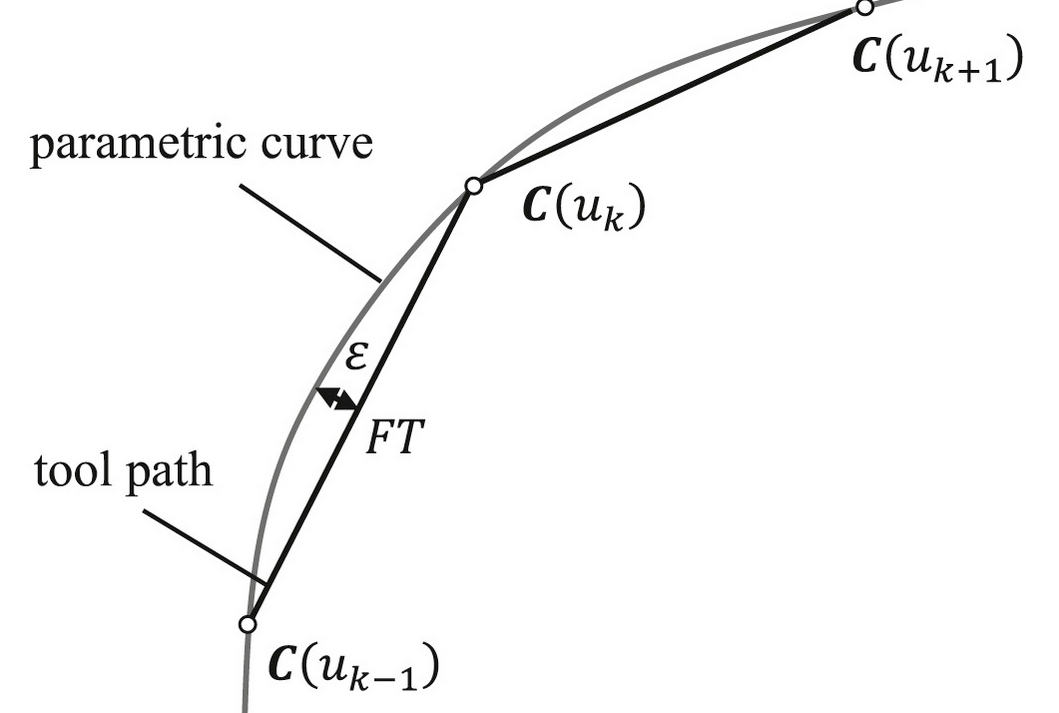
\includegraphics[width=0.80\textwidth]{Images/Chap3/Chord-error-image.png} 
\end{figure}


Generally, for a specific curve path, an increase in feedrate F, will decrease the total number of interpolated points but will increase the chord length (FT), of each arc segment, thereby increasing the chord-error $\epsilon$. \\

On the other hand, a decrease in feedrate will increase the total interpolated points and reduce the chord-error but will cause the overall machining operation to be slow and time consuming. Thus, there is an interplay between chord-error $\epsilon$, and machine feedrate F. The problem is how to find an optimum balance. \\

This work proposed a solution by developing a realtime parametric curve interpolation algorithm that constrains both the feedrate and chord-error simultaneously. It was developed and tested for ten(10) different 2-dimensional parametric curves. \\ 

The curves were selected based on complex shape characteristics like closed loop curves, open ended curves, symmetric or non-symmetric about the x-axis and y-axis. Some curves have sharp, concave or convex turns including cusps. In addition, the x and y dimensions, that is, their overall sizes vary among the different curves. These are some of the geometrical constraints of the algorithm.\\ 

The dynamical and kinematical constraints cover specific CNC machine characteristics like the maximum and minimum allowable machine velocities and accelerations for the different axes of motion, the user specified command feedrate, the jerks and jitter that in combination affects the smooth operation of the machine.  References: \cite{Yeh:2019}, \cite{Yu-etal:2020}, and \cite{Rob:2022}.


\section{Motivation}

Ever since the author was a child, there were always fascinations with regards to moving things and objects, both animated and non-animated. If growth is considered a movement, then humans, animals and plants grow. Whereas the growth of humans and animals are in years, the "growth movements" of vegetation, for example, trees, shrubs and vegetables can be in days, weeks, months and in years, that is, on very different time scales. Humans and animals can move instantly, by choice or instincts. \\

Inanimate objects, though inherently non moving, can be made to move. Manufacturing robots, vehicles, satellites, spaceships, underwater submarines, drones, missiles and Computerized Numerical Control (CNC) machines, are examples of inanimate objects that can move or move others, with the help of motors, hydraulics, electrical, chemical, wind, wave power, and so on. These inanimate objects can move guided or autonomously by some control system, typically but not necessarily using software.\\ 

For example, fighter bombers during the Second World War (early to mid 1940s) were manually controlled using hydraulics by human pilots because there was no software. Thousands of years ago, the ancient Egyptian system for flood and irrigation control of the Nile river uses water wheels and water mills. Software and computing machines were not invented yet so there was no software to use at that time.\\ 

The Apollo Control and Guidance System (ACGS developed by MIT) was a crude combination of basic software, hardware and electronics. The system successfully sent humans to the moon, landed and returned them to earth safely in the late 1960s. This is a very significant landmark in human history.\\ 

In particular, CNC machines for example, move electric motors for cutting drills (milling or engraving), lasers and high pressure water jets to cut materials and produce diverse and useful products for humans. Today, the use of software to control movements of some systems is almost ubiquitous.\\ 

With the author's having access to a bare-bones prototype CNC machine, the interest grew into the complex world of animating non-animated objects. This led to the current endeavor in CNC machine and its control software, the interpolation program. \\

Basically, in order to produce the physical part that is being machined, the interpolation program generates commands that move motor drives step-by-step and point-to-point to follow the desired path or trajectory. \\

Moving inanimate objects is not limited to just cutting things like in the CNC machine. It is also about robots moving around, avoiding obstacles, and performing actions beyond what humans can do, in the air or underwater, in guided or autonomous modes. The possibilities are endless.

\section{Brief description of this thesis}   

\noindent 
The work in this thesis is about mechatronics and system design. The topic in this work covers five(5) major themes described as follows.

\begin{enumerate}
	\item Parametric curve - a special mathematical representation of a path trajectory 
	
	\item Interpolation - the activity of determining the successive "next-points" in following the specified path trajectory
	
	\item Chord-error - the error between the actual "moved" position and its required position according to the specified path
	
	\item Feedrate - the actual speed of motion along the path.
	
	\item Realtime - the current time in execution by point-to-point moves along the path.
	
\end{enumerate}

\noindent
From the above themes, this work is appropriately titled \textbf{"Realtime interpolation of parametric curves with chord-error and feedrate constraints."} \\

\noindent
The next section presents an example of the expected results of this thesis.

\clearpage
\pagebreak

\section{About end results of this thesis} \label{sec-About end results of this thesis}

\begin{figure}
	\caption  {Butterfly Perspective View 3D in LinuxCNC-Axis}
	\label{img-Chap1-Butterfly-Perspective-View-3D-from-LinuxCNC-Axis.png}
	\centering
\framebox{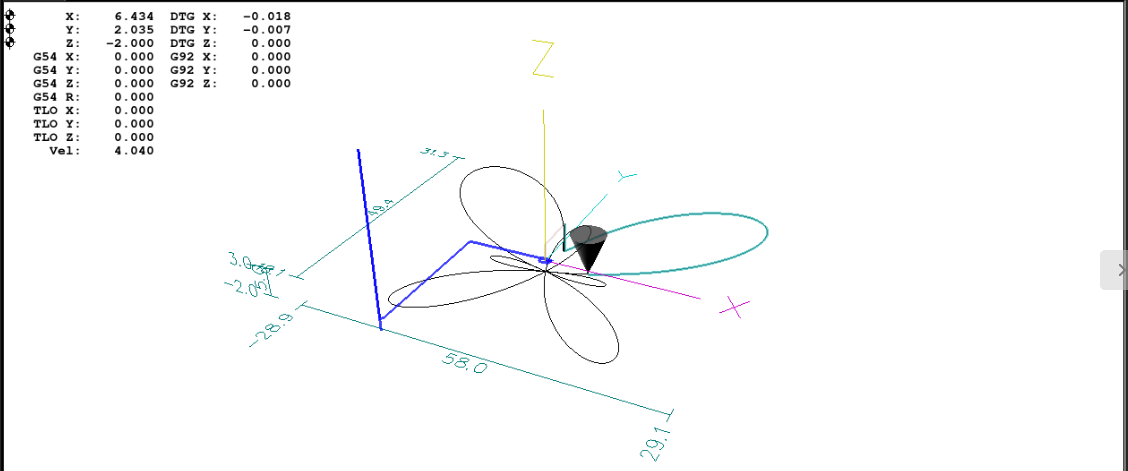
\includegraphics[width=1.00\textwidth]{Chap1/images/img-Chap1-Butterfly-Perspective-View-3D-from-LinuxCNC-Axis.png} }
\end{figure}	

The end results of this thesis can be described as follows. The work in this thesis is about generating a single interpolation algorithm that is successfully applied to ten(10) different parametric curves of various shapes and dimensions. The above figure shows a real live execution of the Butterfly parametric curve (one of the ten curves), by the algorithm developed in this work. \\

The job of the interpolation algorithm is to generate successive points along the curve trajectory so that the CNC cutting tool (laser cutter) illustrated by the cone in the figure follows the path accurately. The curve begins at parameter u = 0.00 (starting point), increasing in steps until u = 1.00 (ending point), as the entire Butterfly curve is being followed, that is, from start to finish. \\

The algorithm uses the second-order Taylor's approximation to calculate the steps (u-next) in parameter u, and at the same time constrains both the chord-error (deviation from the true curve path) to below a set error tolerance (1E-6 mm), and the running feedrate to be very close but below the feedrate limit throughout the full curve path. \\

The feedrate limit at every parameter u point is calculated by the algorithm based on geometrical, dynamical and kinematical constraints. The constraints comprise 4 different components: user set Feedrate Command FC, minimum and maximum CNC machine axial velocities, minimum and maximum CNC machine axial accelerations, and the geometric factors of the curve path like bends and sharp turns. \\

\clearpage
\pagebreak

The main objective of the algorithm execution is to ensure that the resulting running feedrate (speed motion of the cutting tool) is smooth and continuous, and not exceeding the feedrate limit throughout the full curve path. Note that the feedrate limit varies with u, and thus, the running feedrate also varies, for example, when negotiating curves and sharp bends. The algorithm accomplishes the tool motion strictly without violating both the chord-error and running feedrate constraints. \\

Since the smoothness of running feedrate is critical to the success of the algorithm, any acceleration jitters (rapid acceleration fluctuations) will result in jerky machine feedrates. The algorithm execution was able to completely avoid this situation. 

%% =============================================
%% \clearpage
%% \pagebreak

\section{Scope of work for this thesis}

The scope of work for this thesis can be described as follows:

\begin{enumerate}
	\item Selection of ten(10) different parametric curves and their equations, each curve with varying features, shapes and dimensions.
	
	\item Setting up the feedrate (velocity) constraining dynamic equations for allowable CNC machine parameters like the maximum and minimum axial velocities, and maximum and minimum axial accelerations.  
	
	\item Setting up the chord-error constraining equations involving geometric and kinematic properties of the ten(10) different parametric curves.
	
	\item Development of a realtime algorithm that generates interpolated points which traverses each curve, such that the chord-error and feedrate at all points are simultaneously constrained.  
	
	\item Execution of reports that show the interpolation algorithm performs correctly as designed, generating interpolated points and feedrates that are smooth and continuous for all ten(10) parametric curves selected. 
	
	\item In addition, the reports on algorithm implementation show that the absolute constraints on chord-error and feedrate are not violated throughout the full trajectory of each curve. 
	
	\item The execution of the algorithm on all ten(10) curves also show that acceleration jitters do not occur, and the acceleration is always maintained between the designed maximum and minimum limit.   
	
	\item The algorithm also generates RS274/NGC G-Code file for validation and verification on the CNC machine running the LinuxCNC-Axis control application.
	
	\item For the performance assessment of the developed algorithm, four different metrics were created. The four metrics are:
	
	\begin{itemize}
		\item SCE/TIP, that is the ratio of total sum-chord-error divided by the total number of interpolated points.
		
		\item SCE/SCL, that is the ratio of total sum-chord-error divided by the total sum-chord-length.
		
		\item SAA/SCL, that is the ratio of the sum-arc-areas divided by the total sum-chord-length.
		
		\item 100(SAL-SCL)/SAL, that is the ratio of the difference between the sum-arc-length and the sum-chord-length, divided by the sum-arc length and multiplied by 100 to represent it in percentage form.
		
	\end{itemize}
	
	\item The results in the main document of this thesis discuss the full outputs of the Teardrop curve resulting from the algorithm execution. The outputs for the rest of the nine(9) selected curves are provided in their respective appendices.	
	
\end{enumerate}




%% =========================================
\clearpage
\pagebreak

\section{Organization of this thesis document}

Chapter 1 Introduction, covers the basic ideas on parametric interpolation, Computerized Numerical Control (CNC) machines, the G-code standards for these CNC machines, chord-error and machine feedrates associated with CNC machining operations. The introduction also includes the problem statement and the motivations that led to this work. Finally, the organization structure of this thesis is documented.\\ 

Chapter 2 Literature Review, involves the topics on mathematical parametric representation of curves and surfaces in NURBS, the general ideas on $C^{N}$ continuity of curves and surfaces and, the advantages of parametric representations. This chapter also includes the concepts of interpolation of parameteric curves. It is followed by a literature review of published sources for previous works involving interpolation of parametric curves and surfaces. At the end of this chapter, the ideas of NURBS and its relationship to CNC G-code programming languages were discussed.\\

Chapter 3 Methodology, begins with describing the processing steps involved in parametric curve interpolation, and include the characteristics and presentation of mathematical equations for the ten(10) parametric curves selected for this work. It is followed by the discussion on chord-error (epsilon) concepts, the chord-error minimization, feedrate maximization, and the proposed combined chord-error and feedrate constraints to be enforced simultaneously. Next, the criteria of convergence is stated in the brief algorithm design for this work. \\ 

Chapter 3 continues with the mathematical derivations of equations to be computed in the algorithm. This includes equations for the radius of curvature ($rho$), chord-error ($epsilon$), current feedrate ($curr\_frate$). The derivations of the first and second order iterative Taylor's expansion followed. This chapter then continues with the calculations for the next interpolation point. The discussions and equations for the various feedrate limits ($frate\_limit$), consisting of the combined dynamical and geometrical constraints were presented. The main program for the interpolation was described through a flowchart. The equations and flowcharts for the rising and falling of feedrates using the sigmoid S-curves were derived, discussed and presented. Chapter 3 ends with the presentation of a flowchart for the balance of chord-error and feedrate combined constraints. \\

Chapter 4 Results, presents the final outcomes of the entire work for this thesis. Out of the ten(10) parametric curves studied in this work, the full results of only one(1) of those curves, for illustration, are presented in the main document. The full results for the rest rest of the curves (about 20 pages per curve) are provided in the respective appendices. The full results for the rest of the curves can be compiled into a separate, second document, considered an annex to the main document for this thesis.\\

The main results presented in Chapter 4, for the illustrative curve, comprise profiles for feedrate, chord-error, interpolated step size, radius of curvature, feedrate limit constraints, and tangential accelerations. For overall algorithm performance analyses, a comprehensive table collection of execution data was compiled for all of the ten(10) curves. The data comprise important statistics like total interpolated points, the histogram of interpolated points against the parameter range, the histogram of the chord-errors against the parameter range, the feedrate points above and below feedrate limits, the sum total of chord errors (total accumulated error), the sum of chord lengths (total path length traversed for each curve), and so on.\\ 

One interesting performance result for each curve is the ratio of total accumulated error against the total path length traversed. This is a meaningful performance measure for the interpolation algorithm since it measures the amount of chord-error generated by the algorithm per unit length of curve traveled. \\

The total interpolated points is not a meaningful measure because each curve has a different total length. The results also provides trending data for algorithm executions against four(4) different feedrate command (FC10, FC20, FC30 and FC40) values for each of the curve. The interpretation of the total number of interpolated points for each FC value for comparison becomes meaningful.\\

Chapter 5 contains the conclusions of this research, sharing of some lessons learned and recommendations for future work.






\chapter{LITERATURE REVIEW}


\section{Parametric Representation of curves and surfaces}

The standard for describing and modeling curves and surfaces in computer aided design (CAD) and computer graphics is NURBS, or NonUniform Rational B-Splines. Extensive mathematical coverage describing NURBS are found in the seminal books of \cite{Rogers:2001} and, \cite{Piegl-etal:1997}. \\

Essentially, NURBS describe parametric curves and surfaces. Curves and surfaces are mathematically represented either explicitly, implicitly or parametrically. \\

In general, a parametric curve representation of a 3D curve takes the mathematical functional form of $C(x(u), y(u), z(u))$ where $x(u)$, $y(u)$, and $z(u)$ are mathematical functions in the independent parameter $u$, bounded by a range $u_{min}$ $\le$  $u$ $\le$ $u_{max}$.\\
 
By extension, a parametric surface representation of a 3D surface takes the form of $S(x(u,w), y(u,w), z(u,w))$ where $x(u,w)$, $y(u,w)$, and $z(u,w)$ are mathematical functions in two independent parameters $u$ and $w$. The parameters $u$ and $w$ must also be bounded.\\
 
When compared to either explicit or implicit formulations, this parametric representation is extremely flexible. The representation is axis independent, easily represented by multiple-valued functions and, can have infinite derivatives. Furthermore, to have more degrees of freedom independent parameters can be added.\\

In practice, curves and surfaces are generally bounded. When either an explicit or implicit representation is used, imposing the boundaries is awkward. In contrast, the boundaries for a parametrically represented curve or surface are provided by the restrictive parameter ranges. In addition, the parameter range for a parametric curve also specifies a natural traversal direction along the curve. \\

As an example, for a 3-dimensional curve with independent parameter $u$ in the range $u_{min}$ $\le$  $u$ $\le$ $u_{max}$, the curve direction will be from the point $C(x(u_{min}), y(u_{min}), h(u_{min}))$ to $C(x(u_{max}), y(u_{max}), h(u_{max}))$ as $u$ increases from $u_{min}$ to $u_{max}$.\\

Note that specifying a curve requires one parameter while a surface requires two parameters. Also a parametric curve with the function $h(u)$ being zero for all values of parameter $u$ means the curve is 2-dimensional or a curve in the x-y plane.


\section{Continuity of curves and surfaces}

There are two kinds of continuity, or smoothness, associated with parametric curves and surfaces known as geometric continuity $G^{n}$, and parametric continuity $C^{n}$, where $n$ is the order of the derivative. Simplistically, you can think of geometric continuity as physical and parametric continuity as mathematical. Geometric continuity is less restrictive than parametric continuity. This means that if it is $C^{n}$ continuous, then it implies $G^{n}$ continuous, but not the opposite. The fundamental difference between geometric $G^{n}$ and parametric continuity $C^{n}$ can be illustrated as follows. \\

Given a parametric vector-valued function, $P(u)$, over some parameter range $u$ describing a curve, then any given value of $u$ represents a specific point on the curve. The first derivative, $P^{'}(u)$, represents the velocity of a point as it moves along the curve, and the second derivative $P^{''}(u)$ represents the acceleration. \\

If the curve is $C^{1}$ continuous at a join, then both the direction and magnitude of the tangent vector are equal across the join; and the point smoothly transitions from one curve segment to the next. If, however, the curve is only $G^{1}$ continuous at the join, then as the point transitions across the join the direction of motion does not change (tangent vector direction), but there is an instantaneous change in speed (tangent vector magnitude) that represents an instantaneous acceleration as the point transitions across the join. If the curve represents a path trajectory for a CNC machine, the abrupt velocity (magnitude) change will cause a sudden jerk.\\

Note that $C^{0}$ means the parametric continuity of the curve itself, and $C^{1}$ and $C^{2}$, the continuity of its first and second derivatives, respectively. All of the parametric curves selected and used in this work are $C^{2}$ continuous.

%% =======================================================
\clearpage
\pagebreak
\section{Computerized Numerical Control (CNC) Systems}

A typical machine architecture for a 3D-four-axis machine is shown in Fig [\ref{CNC-Basic-Architecture.png}]. The 3D axes corresponds to the x, y, and z motion axes while the fourth is the rotating axis of the spindle cutting tool. Fig [\ref{CNC-Servo-and-Spindle-Driving-Mechanism.png}] shows the mechanism of the axial motions and the rotational motion of the spindle while Fig [\ref{CNC-Typical-Software-Control-Flow-Diagram.png}] shows the typical software control flow diagram for a typical CNC machine.\\


CNC manufacturing operations involve the generation of reference signals describing the geometrical parts to be machined and the control of the machine such that it follows those reference signals. In modern CNC machines, the generation of reference signals, construction and execution of control loops are accomplished in software within a computer. Fig [\ref{Functional-Architecture-of-CNC-System.png}] shows the block diagram for the functional architecture of a typical CNC system.\\

%% \noindent
A modern commercial CNC 3D-four(4)-axis milling machine is shown in Fig [\ref{CNC-Commercial-Milling-Machine.png}]. The fourth axis is the rotational axis for the spindle cutting tool. An example of a a commercial CNC lathe machine is shown in Fig [\ref{CNC-Commercial-Lathe-Machine.png}]. Modern commercial CNC machines today have extended milling and turning to 9-axes, for example, the DN Solutions PUMA SMX3100ST combined milling and turning machine. \cite{TitanCNC:2021} shows a YouTube video of this 9-axes CNC in action.\\


\begin{figure} 
	%%	\centering
	\caption{Basic achitecture for a typical CNC system}
	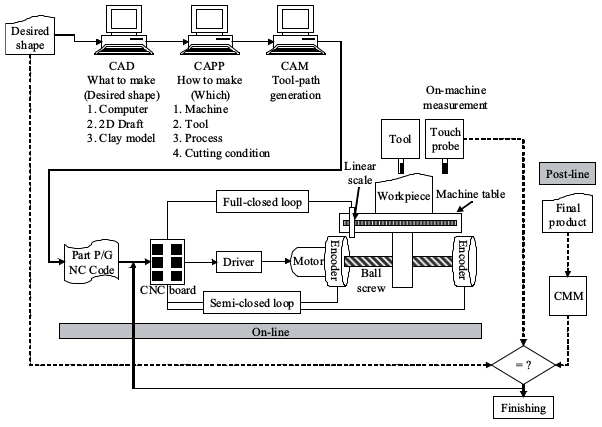
\includegraphics[width=0.90\textwidth]{Chap2/Images/CNC-Basic-Architecture.png} 
	\label{CNC-Basic-Architecture.png}
\end{figure}

%% ==========================================
\clearpage
\pagebreak

\begin{figure}
	%%	\centering
	\caption{Typical Servo drive and spindle driving mechanism}
	\label{CNC-Servo-and-Spindle-Driving-Mechanism.png}
	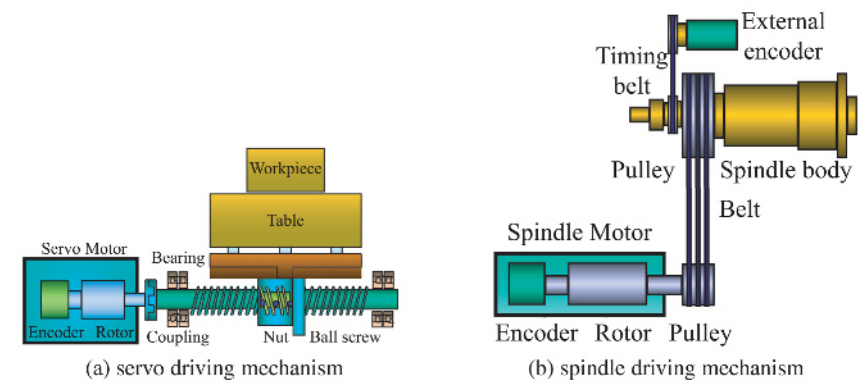
\includegraphics[width=1.00\textwidth]{Chap2/Images/CNC-Servo-and-Spindle-Driving-Mechanism.png} 
\end{figure}



\begin{figure}
	%%	\centering
	\caption{Typical CNC Software control flow diagram}
    \label{CNC-Typical-Software-Control-Flow-Diagram.png}	
	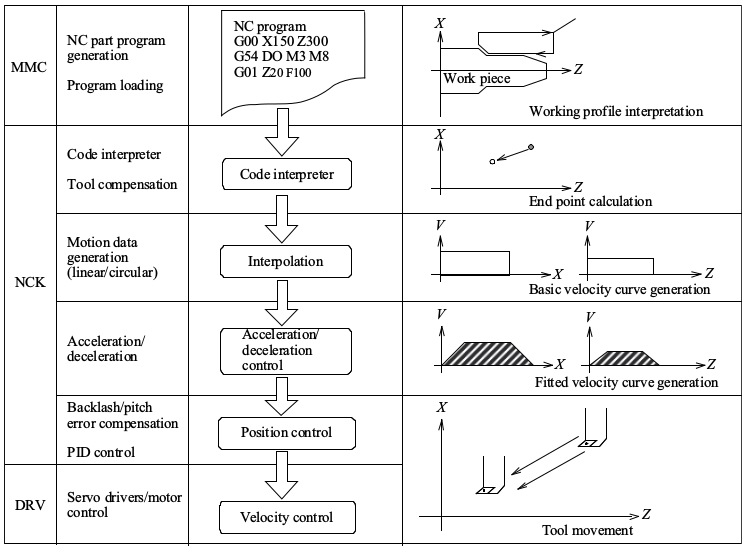
\includegraphics[width=1.00\textwidth]{Chap2/Images/CNC-Typical-Software-Control-Flow-Diagram.png} 
\end{figure}

\clearpage
\pagebreak

\begin{figure}
	\centering
	\caption{Typical CNC Functional Architecture}
	\label{Functional-Architecture-of-CNC-System.png}
	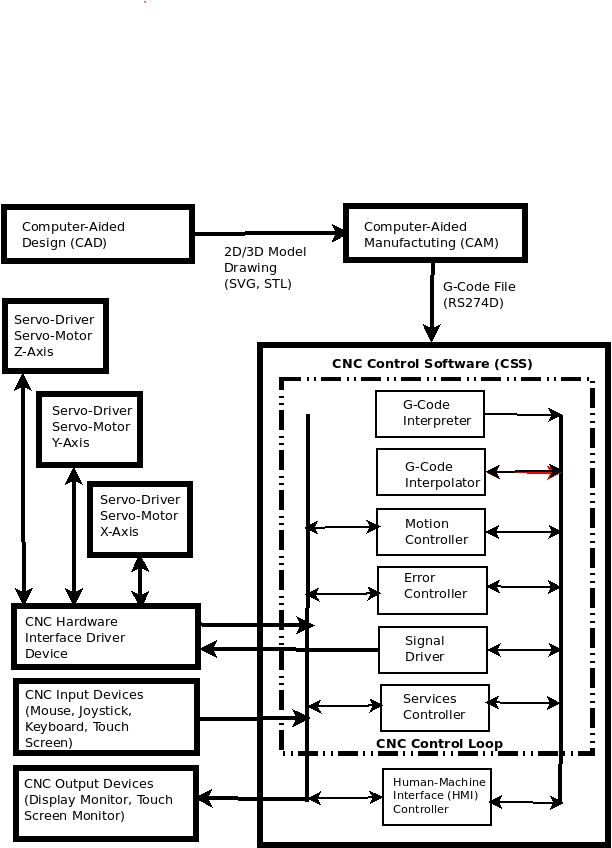
\includegraphics[width=1.00\textwidth]{Chap2/Images/Functional-Architecture-of-CNC-System.png} 

\end{figure}


\clearpage
\pagebreak
\begin{figure}
	\centering
	\caption{Typical CNC Commercial Milling machine}
    \label{CNC-Commercial-Milling-Machine.png}	
	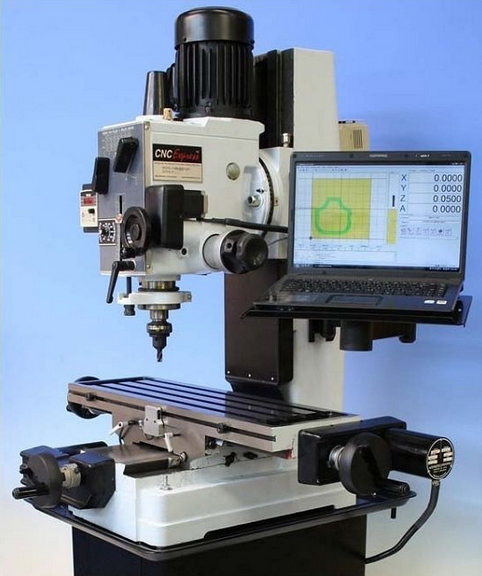
\includegraphics[width=1.00\textwidth]{Chap2/Images/CNC-Commercial-Milling-Machine.png} 
\end{figure}

\clearpage
\pagebreak
\begin{landscape}
\begin{figure}
	\centering
	\caption{Typical CNC Commercial Lathe machine}
    \label{CNC-Commercial-Lathe-Machine.png}	
	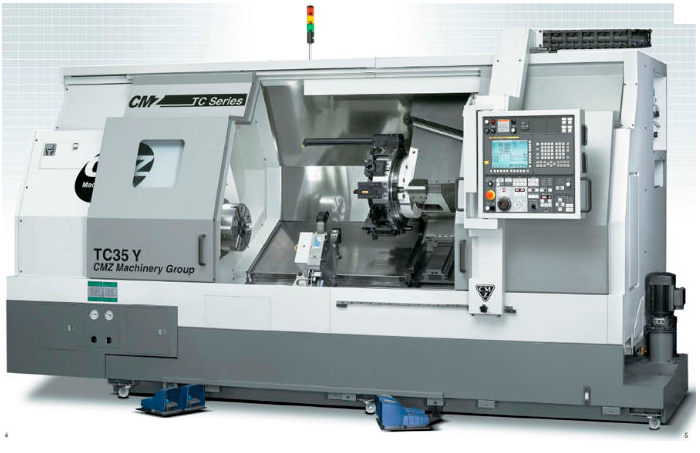
\includegraphics[width=1.40\textwidth]{Chap2/Images/CNC-Commercial-Lathe-Machine.png} 
\end{figure}
\end{landscape}



%% ===========================================================
\clearpage
\pagebreak
\section{Advantages of Parametric Representations in CNC}

Parametric interpolation has many merits over the traditional linear (G01) and circular interpolation (G02 and G03) in terms of model representation, feedrate smoothness and application range. \cite{Jin-etal:2014} reported some advantages below.\\

\begin{enumerate}
	\item In parametric interpolation, the geometrical information of the machining paths can be totally as well as accurately transferred to the CNC systems without any approximation errors and data loss. This error and loss may occur in conventional linear and circular interpolation.
	
	\item The parametric interpolator code only needs some critical parameters of the machining contours (i.e. control points, knot vectors, weights as in NURBS). Such a transmission mechanism can guarantee the efficiency of interaction between the host and slave machines.
	
	\item In parametric interpolation, feedrate continuity and smoothness are achieved effectively since the joints between tiny segments do not require repeated acceleration–deceleration processes. In traditional interpolation methods repeated acceleration–deceleration may not be avoidable.
	
	\item Parametric interpolation is still possible in conventional CNC systems after some developments of the machining parts. This may include approximating tiny parts into curve segments and optimization with parametric curves between them.
\end{enumerate}

%% ======================
\clearpage
\pagebreak

\section{Interpolation of parametric curves}

The problem statement for interpolation of a parametric curve is: \\

\textit{Given the parametric curve $C(u)$, determine $u(k)$ for the $k_{th}$ interpolation period, the re-parametrization of $u$ with time $t$ is required, that is, solve the function $u = u(t)$, where $u$ is the independent parameter, and $t$ is time.}\\

In other words, it means at a point on the parametric curve $C(u)$, find the next $u$ point. The next $u$ point is a function of time $t$.\\

Since the machine moves with time, the re-parametrization from $t$ to $u$ should be subjected to the machine dynamic constraints and contour error tolerance. It can be described as follows. 

\begin{enumerate}

\item The machine axial velocities and accelerations should be limited to avoid saturating the axes. These are the first and second derivatives of the corresponding parametric function $C^{'}(u)$ and $C^{''}(u)$ with $u = u(t)$, over time, respectively. 

\item The limitations include satisfying specific machine characteristics like startup torque, maximum and minimum velocity (feedrate), maximum and minimum acceleration (jerk), and encoder resolution (incremental motion stepping). 

\item In order to guarantee a smooth trajectory motion profile the jerk should be limited or completely eliminated. This ensures a smooth feedrate profile.  

\item The contour error $\epsilon$ increases with increasing feedrate, so the feedrate should be limited to achieve high contour accuracy. There should be an optimum strategy to balance contour error and machine feedrate.

\end{enumerate}

The function of the real-time interpolator in a computer numerical control (CNC) machine is to compute a reference point in each sampling time interval T (for example, 0.001 s), of the servo system, based on a prescribed tool path (curve) and feedrate data. \\

By comparing the actual instantaneous machine position (measured by encoders on the machine axes) with the reference point, accurate closed-loop control of the machine position and speed may be obtained.\\




%% ======================
\clearpage
\pagebreak

\section{Previous works on parametric interpolation}


Probably, \cite{Koren:1976} was the first to introduce the general concept of interpolation for a {CNC} system.  Later, \cite{Koren-etal:1993} and \cite{Shpitalni-etal:1994} extended the idea to basic approximation principles for parametric curves. \\

The two common technical routes that have been developed for the interpolation of parametric curves are the arc length parametrization and the recursive/iterative Taylor's expansion. \\

It was reported by \cite{Farouki-etal:2001} that near arc length parametrization is possible with some numerical methods. However, it is computationally intensive with the approximation error accumulating along the curve. This especially occurs in curves with large curvature variations like sharp turns, and with uneven parameter computations.\\

In order to realize parametric interpolation, researchers developed a wide variety of methods to achieve better machining qualities. The common adopted approaches for interpolating parametric curves were based on Taylor’s expansion, for example, \cite{Cheng-etal:2002}.\\

\cite{Farouki:2021} considered realtime interpolators based on Taylor series to possess two inherent shortcomings. Firstly, the occurrence of truncation errors because only a finite (small) number of terms can be employed, and secondly, for variable feedrates, the coefficients of higher-order terms, defined by successive chain-rule differentiation, become increasingly complex and cumbersome, especially when involving computationally intensive expressions.\\

A parametric interpolation method based on prediction and iterative compensation was proposed by \cite{Ni-etal:2019} where the feedrate fluctuation and Taylor’s expansion were analyzed to reduce the calculation accuracy of truncation errors caused by neglecting the high-order terms. \\

Another method for parametric interpolation is named 'guide curve based'. It was developed by \cite{Sun-etal:2006}. This method implements the near arc length parameterization. Essentially, the detection of corners and key regions are done offline, and this approach schedules feedrate based on a guide curve without a look-ahead facility. \\ 

\clearpage
\pagebreak


Although available CNC interpolators for parametric curves generally achieve contouring position accuracy, the specified feedrate, which dominates the quality of the machining process, is not guaranteed to be smooth during motion. Severe speed fluctuations may incur tool chatter or breakage, especially in high speed machining. Since feedrate control is crucial, \cite{Yeh-etal:1999} for example, developed a speed-controlled interpolator for machining parametric curves. \\

Later, \cite{Yeh-etal:2002} considered interpolation of parametric curves by adapting the feedrate with a confined chord error while  \cite{Nam-etal:2004} proposed an approach for parametric interpolation that allows the feedrate profile to be dynamically adjusted according to geometrical path constraints. \\

Tracking error and contour error are two very important aspects that need to be effectively handled by any CNC servo control system.  \cite{Ramesh-etal:2005} reviewed the various techniques that have been developed in minimizing and eliminating tracking and contour errors.\\ 

A much later review, 13 years after, was conducted by \cite{Jia-etal:2018} on the subject of contouring-error reduction method in multi-axis CNC machining. The review covers both three-axis and five-axis contouring-error reduction methods. The methods comprise various offline contouring-error reduction, interpolator designs for contouring-error reduction, cross-coupling schemes for direct contour control and contour control algorithms. As an example, \cite{Chen-etal:2019} considered contour error-bounded parametric interpolator with minimum feedrate fluctuation. \\

The paper by \cite {Lee-etal:2018} reviews recent progress of control technologies for precision machining using CNC in the area of interpolation, contour control and compensation. In terms of interpolation several corner blending methods and parametric curves are introduced and the characteristics of each method discussed. In addition, contour control algorithms recently developed for multi-axis machines are also reviewed.\\

In another direction, \cite{Bhattacharjee:2012}, instead of using Taylor's expansion approximation, employed the classical fourth-order Runge-Kutta (RK) method using only the first derivative to generate successive parameter values for the calculation of x, y, z coordinates of interpolated points. It was done in order to avoid calculating higher derivatives and make the interpolation calculations simpler.\\

\clearpage
\pagebreak

On parallel implementation, \cite{Fu:2016} developed a parallel CNC system architecture based on Symmetric Multi-Processor (SMP). This  subject is of interest to this author. The author's involvement on parallelism in CNC is discussed in the next section, where FPGA (Field Programmable Gate Arrays) programming was used to drive the CNC machine.\\


\section{Related CNC work by the author}

Low end research CNC machines, like the CNC UMP Model 2008 in Fig [\ref{chap2-CNC-Research-Machine-3-Axis.jpg}], can be controlled and driven using small devices and (IoT) gadgets, like desktops, laptops, computer extension boards and single-board-computers (SBC).\\ 

\cite{Kalimbetov:2012} used C/C++ and Python codes on a Linux box driving the UMP CNC model 2008 machine in realtime using a customized parallel port software driver. Comparisons were conducted running the CNC on both realtime (RTOS) and non-realtime (NRTOS) operating systems. \\

\cite{Ariffin:2014} used the USB based Arduino Due extension board to drive the UMP CNC machine. This resource limited hardware (only 512 KB onboard user Flash memory) required a special technique in writing the C/C++ codes for the CNC software driver.\\  

\cite{Abdelgader:2014} used a combination of gadgets to drive the CNC machine, using the computer laptop, the proprietary Heber X10i extension board and the Raspberry Pi 2 single board computer (SBC). The Raspberry Pi a low cost, credit-card sized, full board computer was successfully used to drive the CNC machine. Since, the memory addresses of the driving pins in the Heber X10i hardware are separated, a special technique was developed to get the memory register addresses contiguous. \\

\cite{Ahmad:2017} later used the Raspberry Pi 3 Model B, an updated version to drive a CNC machine in Real Time. An output for this work is shown in Fig [\ref{Thank-You-WRY-Asyrul.png}]. The step by step CNC process from start to finish (capture image, convert image to G-code, drive G-code on UMP CNC machine) executed by \cite{Ahmad:2017} is shown in an interesting video accessible at the link: [\href{https://www.youtube.com/watch?v=4s94wy6ZGJE}{CNC Rpi3 Real Time, 5m:46s}]. The video is demonstrated with a beautiful background rendition of the song "Jalur Gemilang", a snapshot of it is provided in [\ref{chap2-CNC-Jalur-Gemilang-Rendition-Video.png}].

\clearpage
\pagebreak

\cite{Selvarajah:2015} deployed the Beagle Board xM single board computer (SBC), to drive the CNC machine. This Beagle Board xM is a variation of SBC gadgets with more capabilities than the Raspberry PI. This board used the OMAP (Open Multimedia Applications Platform) processor, which is capable of video and image processing. OMAP is mostly used in commercial cell phones.\\ 

The highlight is the work of \cite{Teh:2016} that engaged the Nexys-3 Spartan-6 FPGA board to develop a closed-loop feedback system that controlled the CNC machine. An image of this quite expensive board is provided in Fig [\ref{Nexsys3-Spartan6-Xilinc-board.jpg}] at the bottom right. the green board with a USB-UART connection. \\

FPGAs are truly parallel in nature, so different processing operations do not have to compete for the same resources. In addition, the inherent parallel execution of FPGAs allows for independent pieces of hardware logic to be driven by different clocks. Depending on design, FPGA processors execute multiple tasks at any one time. This is unlike typical Intel x86 or ARM processors that execute line by line.\\

FPGAs are powerful pieces of technology that allow users to implement custom hardware (not software) designs. There are several FPGA programming languages available, but the four most popular are VHDL, Verilog, SystemVerilog, and C/C++. \\

This project utilized a mixed of VHDL and C/C++ languages to program the Nexys-3 hardware that generated the CNC driver codes on the the board. A G-code file on the computer was first converted to a signal file, reference Fig [\ref{Gcode-left-to-Nexys3-signal-file-right.jpg}]. Then, the file is transmitted from the computer to the Nexys-3 board via USB-UART serial protocol. The received signals are then sent by the Nexys hardware to the three(3) x, y, z axial motors of the CNC machine, with the three tasks running parallel in time. Since parallel execution is natural to FPGA operation, the project goal of true parallelism was achieved.\\

Real live Youtube videos of successful CNC executions can be accessed at the following links:  
[\href{https://www.youtube.com/watch?v=3GuhE5dlcYk}{CNC FPGA-Video1, 0:56s}], 
[\href{https://www.youtube.com/watch?v=VvAyLqt\_wLQ}{CNC FPGA-Video2, 0:58s}] and 
[\href{https://www.youtube.com/watch?v=gvlKlqfEXro}{CNC FPGA-Video3, 4m:00s}]. \\

The acquired detailed knowledge, skills and understanding of these diverse raw hardware and their environments, as mentioned in the projects above, is critical to the success of the present author's thesis.\\ 

%% ==================================
\clearpage
\pagebreak

\begin{figure}
	\caption{ CNC UMP Model 2008 - University Malaysia Pahang}
    \label{chap2-CNC-Research-Machine-3-Axis.jpg}
	\centering
	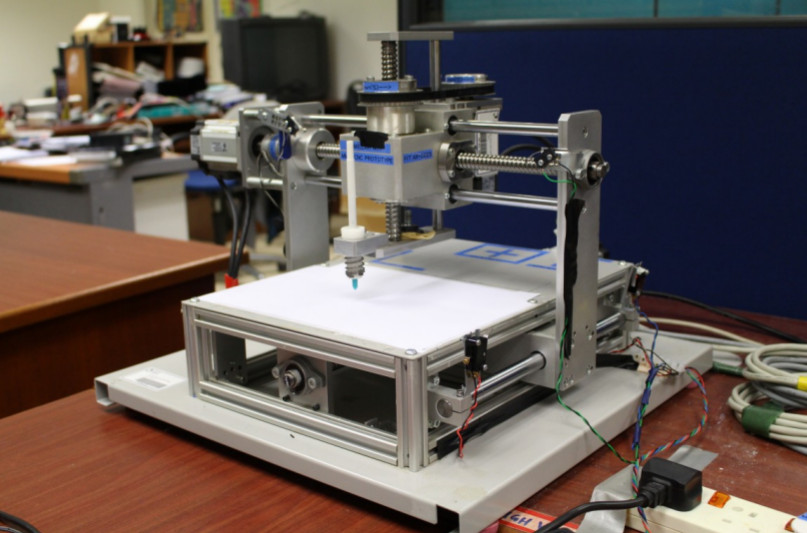
\includegraphics[width=0.95\textwidth]{Images/Chap4/CNC/CNC-Research-Machine-3-Axis.jpg} 
\end{figure}


\begin{figure}
	\caption{Youtube: CNC Jalur Gemilang Rendition Video by Ahmad (2017)}
	\label{chap2-CNC-Jalur-Gemilang-Rendition-Video.png}
	\centering
	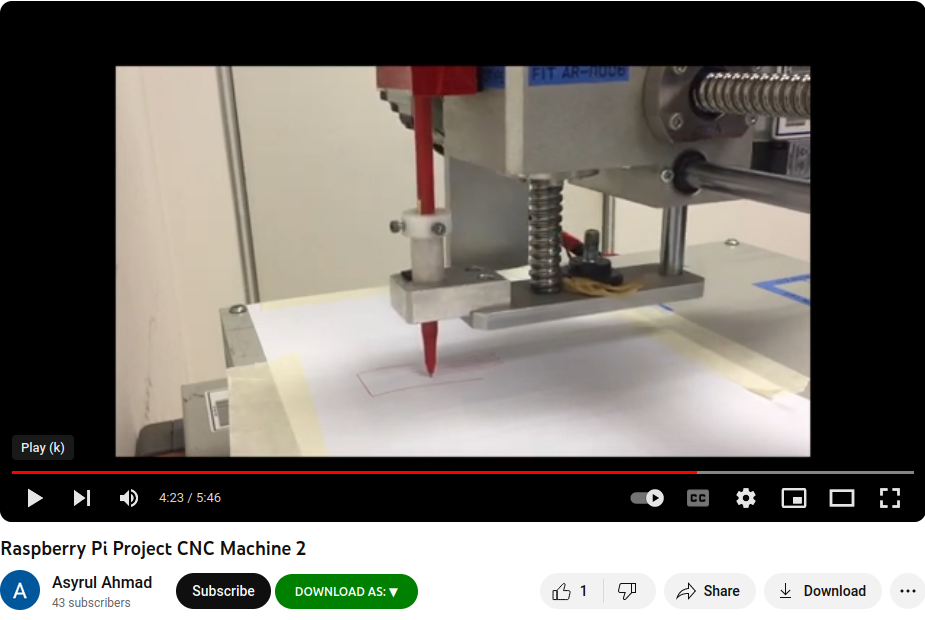
\includegraphics[width=0.95\textwidth]{Images/Chap3/CNC-Jalur-Gemilang-Rendition-Video.png} 
\end{figure}

%% ===================================
\clearpage
\pagebreak

\begin{figure}
	\caption{Proton logo output of UMP CNC machine by Ahmad:2017}
	\label{Thank-You-WRY-Asyrul.png}
	\centering
	
\includegraphics[width=0.95\textwidth]{Chap2/Images/Thank-You-WRY-Asyrul.png} 
\end{figure}

\begin{figure}
	\caption{Setup of Nexsys-3 Spartan-6 Xilinc board by Teh:2016}
	\label{Nexsys3-Spartan6-Xilinc-board.jpg}
	\centering
	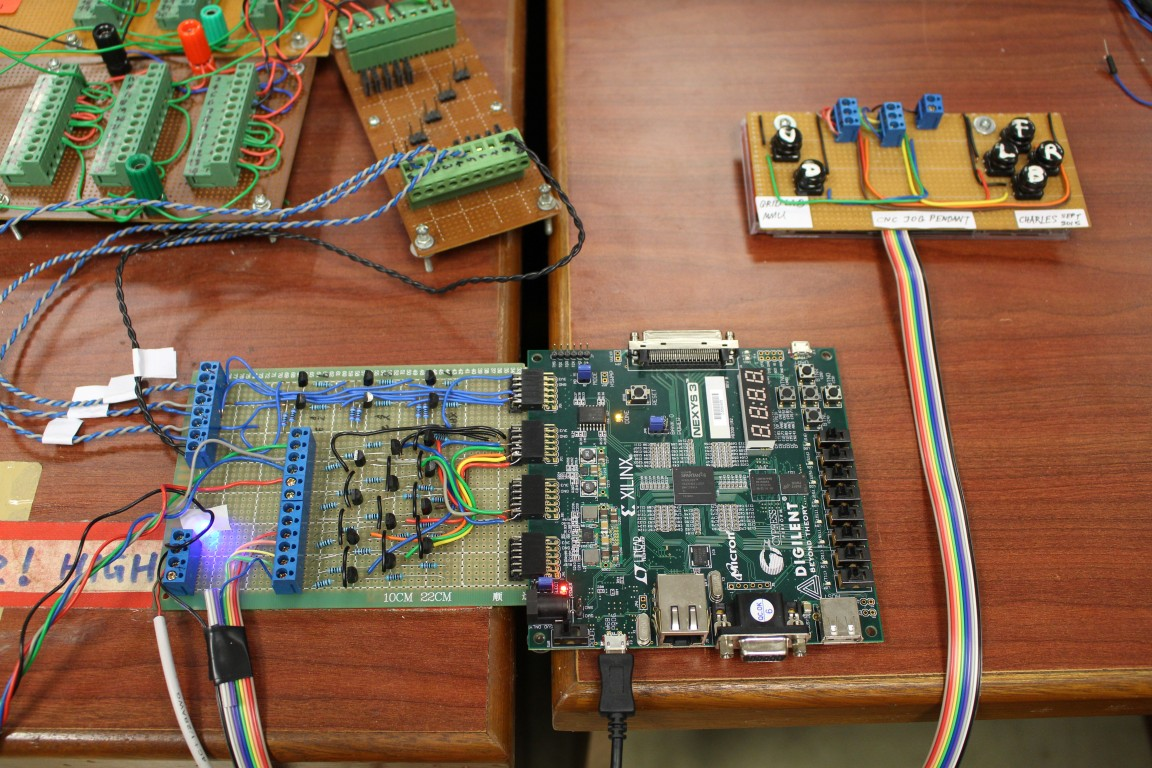
\includegraphics[width=0.95\textwidth]{Chap2/Images/Nexsys3-Spartan6-Xilinc-board.jpg} 
\end{figure}

%% ======================
\clearpage
\pagebreak

\section{Comparisons previous works with this thesis}

Previous works had definitely looked into the issues of chord-error and feedrate in parametric curve interpolations, but in a different perspective compared to the work in this thesis. \\

The early paper by \cite{Yeh-etal:1999} formulated real-time CNC interpolators for variable feedrates along parametric curves. Later, \cite{Farouki-etal:2001} pointed an erroneous coefficient for the quadratic term in the paper. \\

It was mentioned by \cite{Farouki-etal:2001} that, Pythagorean-hodograph (PH) curves admit closed-form analytic reductions of the interpolation integral, yielding real-time interpolators that are essentially exact, and remarkably versatile in terms of the repertoire of feedrate variations (with time, arc length, or curvature) they accommodate. The work in this thesis, also involves feedrate variations with time, arc length, and curvature however, it does not involve Pythagorean-hodograph (PH) curves. \\

\cite{Farouki:2021} considered the successive applications of the differentiation chain rule which are necessary to determine Taylor series coefficients beyond the linear term as being cumbersome, so the use of Richardson extrapolation as a simple means to compute rapidly convergent approximations to the higher-order coefficients was introduced. The work in this thesis, however, does not involve Richardson extrapolation. \\

The work by \cite{Jin-etal:2014} breaks parametric interpolation into rough interpolation and fine interpolation. According to \cite{Jin-etal:2014}, rough interpolation is about feedrate adjustments between two successive interpolation periods, while fine interpolation is about adjusting the feedrate to comply with the geometrical constraints and kinematical characteristics of the CNC machine. The work in this thesis however, implements feedrate adjustments immediately in one interpolation period taking into account of both  geometrical and kinematical constraints simultaneously. \\

The work by \cite{Zhong-etal:2018} does not impose an upper or lower limit for the chord-error. The values of chord-error are considered as whatever resulting from the algorithm running at the particular feedrate. In addition, \cite{Zhong-etal:2018} also allows for feedrate speedup to the value of command feedrate, for example, when it forsees a near straight line coming ahead, and this breaks the absolute feedrate limit constraint. 

\clearpage
\pagebreak

As a comparison, the work in this thesis imposes an upper limit for the chord-error, and strictly preserves both the chord-error and feedrate limit constraints at every point on the curve path, simultaneously. In addition, for feedrate smoothness throughout the entire traversal of the curve path, this thesis imposes a strict condition that does not allow acceleration jitters. This was not a condition mentioned in previous cited works. 


%% ======================
%% \clearpage
%% \pagebreak

\section{NURBS and G-Code programming}

NURBS are a type of spline, which is a curve or surface defined by a set of control points and a basis function. Unlike other splines, NURBS can have rational weights associated with each control point, which allow them to represent conic sections and other shapes that are not possible with polynomial splines. NURBS also have the advantage of being invariant under affine transformations, such as scaling, rotation, and translation, which makes them easier to manipulate and transform. NURBS can also be used to approximate any shape with arbitrary precision, by adjusting the number and position of the control points and the degree of the basis function. Reference: \cite{CollabCNC:2023A}\\

One of the main challenges of using NURBS in CNC programming is the compatibility and interoperability between different software and hardware systems. Not all CAD/CAM software can export or import NURBS data, and not all CNC machines can process or interpret NURBS data. Therefore, you may need to use different formats, standards, or protocols to exchange NURBS data between different platforms, such as IGES, STEP, DXF, or G-code. Another challenge is the quality control and verification of the NURBS data and the machined parts. You may need to use special tools or methods to check the accuracy, smoothness, and consistency of the NURBS data and the output, such as error analysis, simulation, or inspection. \cite{CollabCNC:2023B} discusses how to evaluate the accuracy and quality of NURBS machining results.\\

Low end CAD/CAM systems do not generate NURBS G-Code. However, NURBS have been used by high end systems CAD systems for some time. That is the main reason why it is natural that CNCs should be able to employ tool paths that are also defined in terms of NURBS.\\

This work covers only RS274D NGC G-Code files because the format is the base standard for G-Codes supported by all machines used in the CNC industry. This work does not include Scalar Vector Graphics (SVG) or STereoLithography (STL) files generated by CAD applications. It also excludes the generation of G-Codes from CAM processing of SVG or STL input files.\\

Using NURBS interpolation requires a CNC machine capable of handling NURBS G-Code generated tool paths. Since the NURBS G-Code format is proprietary and only used in the high end FANUC CNC machines. It should be noted that NURBS G-Code files are not the same as NURBS interpolation method. \cite{CollabCNC:2023A}, for example, discusses on how to integrate NURBS with other CNC programming methods and techniques.\\ 

Very recently, as of July 17, 2023, \cite {Hu-etal:2023} published a method for calculating interpolation points of NURBS curves based on chord length-parameter ratio. \\

The construction and manipulation of NURBS geometries is based on a structure with the following fields:
\singlespacing
\noindent
(1) number: the number of control points.\\
(2) coefs: control points coordinates (for NURBS also the weights).\\
(3) order: the degree plus one.\\
(4) knots: the knot vector in each direction

\section{Programming Languages for NURBS}

Traditionally, NURBS algorithms were developed using compiled C and C++ programming languages which are tedious and complicated to setup and use. It is available at the link [\href{https://www.nar-associates.com/nurbs/c_code.html}{C-Codes for NURBS}]. \\

\cite{Bingol-etal:2018} developed the \textit{NURBS-Python} library, a scripted, object-oriented, open-source pure Python library without external dependencies. This open-source library availability provides access for researchers to develop NURBS applications. It is provided at the link [\href{https://nurbs-python.readthedocs.io/en/5.x/}{Python-NURBS Website}] \\

Julia NURBS code is provided at the link [\href{https://github.com/eOnofri04/NURBS.jl}{Julia NURBS library at Github}] since Feb 20, 2019. Octave-NURBS is a collection of routines for the creation, and manipulation of Non-Uniform Rational B-Splines (NURBS), the latest release was on 2021-03-29. It is provided at link [\href{https://gnu-octave.github.io/packages/nurbs/}{Octave NURBS Website}]. \\

Note that, NURBS G-Code will not be in the scope of this research.  In this thesis, to drive the CNC machine, the approach is to adopt the second-order approximations of Taylor’s expansion, in an algorithm where the feedrate is calculated based on the value of chord-error and machine dynamic variables. The end objective is to constrain both chord-error and feedrate. For each point on the curve, the interpolation algorithm is computed in an iterative and recursive manner, back and forth, until it reaches a specified convergence criteria. \\

The interpolation algorithm in this work also generates a RS274D/NGC G-Code for each curve that later can be simulated offline, or executed directly on the UMP CNC machine to verify its success. 


%% ==============================================
\clearpage
\pagebreak
\begin{landscape}

\begin{figure}
	\caption{G-code file (left) and Signal file (right) for FPGA by Teh:2016}
	\label{Gcode-left-to-Nexys3-signal-file-right.jpg}
	\centering
	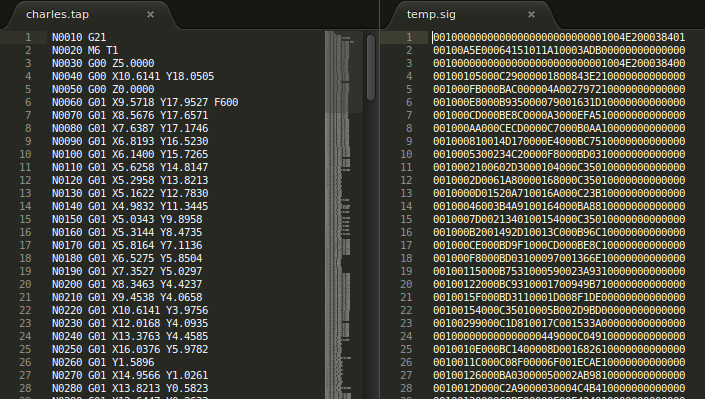
\includegraphics[width=1.62\textwidth]{Chap2/Images/Gcode-left-to-Nexys3-signal-file-right.jpg} 
\end{figure}

\end{landscape}
\chapter{METHODOLOGY}
\label{ch:tocloft}

\section{Parametric Curve Interpolation}

This work involves the realtime interpolation of parametric curves with chord-error and feedrate constraints. The steps required are as follows:

\begin{enumerate}
	\item Obtain the mathematical equations of functions describing the parametric curves.
	
	\item Establish the relationship between the parametric curve, chord-error and machine feedrate in CNC terms. 
	
	\item Understand and formulate CNC machine dynamic and kinematic constraints.
	
	\item Develop and execute a realtime algorithm that satisfies chord-error and feedrate constraints when run on the CNC machine.
	
	\item Generate a RS274D NGC G-code for run simulations and offline execution of the algorithm.

\end{enumerate}
  
%% \clearpage
%% \pagebreak

\section{Selection of parametric curves}

\begin{table}[ht]
%% \begin{center}
\caption{List of ten(10) selected parametric curves}
\label{List-of-selected-parametric-curves}
\begin{tabular}{ p{1.00cm} p{11.0cm}}
\hline
	1  & Circle curve\\
	2  & Ellipse curve \\   
	3  & Teardrop curve  (illustrative curve)\\   
	4  & Butterfly curve \\
    5  & Snailshell curve \\
    6  & Skewed-Astroid curve \\
    7  & Ribbon-10L curve \\
    8  & Ribbon-100L curve (10 times scale up of Ribbon10L curve)\\	
	9  & AstEpi curve (Astroid and Epicycloid curves combined) \\   
    10  & SnaHyp curve (Snailshell and Hypotrocoid curves combined)\\   
\hline
\end{tabular}
\end{table}

% =====================================
%% \clearpage
%% \pagebreak

The parametric curve in this work is a 2-dimensional curve of the type $C(x(u), y(u), z(u))$ where $z(u)$ is zero for all values of $u$. \\

All of the selected curves are at least $C^{2}$ continuous, meaning the second order derivative of $C(u)$ with respect to $u$ must exist. It can be a constant but non zero for the range entire $u$ range.\\

The selection of various parametric curves is aimed at obtaining curves with different features, shapes and dimensions. The curve characteristics cover variations, for example, in size of x and y dimensions, origin or not-origin centered, closed or open ended curves, number of loops, convex or concave segments, sharp or smooth turns, and reflection symmetry about the x and y axes.

%% =======================================
%% \clearpage
%% \pagebreak

\section{Computing challenges in the algorithm}

The main objective of selecting various complexities of parametric curves is to ensure that a single interpolation algorithm to be constructed can handle those complexities in computation without fail. In addition, the various shapes, sizes and features will impose a wide range of computing challenges to the algorithm.\\

Computations must be accurate and efficient. For sufficient precision, computations are conducted using 64-bit machines, and variables are specified in IEEE 754 double-precision binary floating-point format. This gives a precision of up to 15 to 17 significant decimal digits.\\ 

For example, the machine-epsilon (technically known as macheps) in this work is between $1.11 (10)^{-16}$ and $2.22 (10)^{-16}$. Any non-zero number below macheps  is treated by the computing machine as technically zero. This is one of the many challenges in the algorithm especially when computing with very small real numbers. Note that precision is the number of digits specified, while accuracy is the difference of a number from its true value. \\

As an example, a curve that is x-axis symmetrical but not origin-centered will require the algorithm to handle both x and y offsets internally and invisibly. This is an additional challenge.\\ 

In this work, the Teardrop is considered the illustrative curve that provides many features like symmetry, closed-loop, smooth convex arc segments, a sharp pointed edge and varying width. It has all of the important elements to be handled by the interpolation algorithm. This is already considered complicated in comparison to a standard perfect circle which only has two features, that is, a center point and and a constant radius. \\


For example, in this work, a perfect circle with a radius of 79 was selected instead of 80, a number rounded to multiples of 10 (decimal). This prime number 79 (which can only be divided by one and itself), is expected to impose computing challenges mathematically. It is also expected that in computing the successive interpolated points on the circle, it will produce a constant value of 79 for the radius of curvature, $rho(u)$, over the entire range of parameter $u$. This is one of the many verification checks of the algorithm. 


\clearpage
\pagebreak

The Ellipse curve was selected because the Ellipse is essentially like a circle, but elongated vertically to be slim and tall. This feature is just a simple deviation from the perfect roundness of a circle. \\

In the same manner, because the Snailshell curve spirals inward, the radius of curvature $rho(u)$ must be gradually and continuously decreasing, \\ 

Specifically, the two parametric curves for Ribbon10L and Ribbon100L were deliberately sized to be 10 times of each other. This is to check the validity of the interpolation algorithm on scaling. This up-scaling must be handled correctly by the algorithm. Additionally, these two curves are open-ended. In both cases it must be ensured that the algorithm really stops at the correct final positions.\\

The Skewed-Astroid curve was selected to have the algorithm handle four cusps at its corners. Instead of having a standard Astroid curve that is origin-centered and symmetrical about both the x and y axes, the Astroid curve was deliberately skewed to have a tall shape and very sharp cusps. It is very important that the algorithm handles points at these cusps correctly.\\ 

Combinations of standard curves were made to add complexity to the interpolation algorithm. The "AstEpi curve" is a combination of Astroid and Epicycloid curves while the "SnaHyp curve", is a combination of Snailshell and Hypotrocoid curves.
 
%% ======================================================
%% \clearpage
%% \pagebreak

\section{Characteristics of selected curves}

Except for the two curves Ribbon-10L and Ribbon-100L, all other parametric curves listed for $x(u)$ and $y(u)$ involve a single parameter $u$ on the right hand side (RHS) of the equations. These two curves require the $u$ parameter range be normalized to $u  \in  [0.0, 1.0]$. The normalization procedure ensures that the interpolation algorithm cater only a single parameter range $u  \in  [0.0, 1.0]$, which must be applicable to all selected curves.\\

For example, the normalization for curves introduces a new parameter $t$. Firstly, a mathematical function $t(u)$ transforms the parameter $u$ to $t$. Finally, this parameter $t$ is used in the functions $x(t)$ and $y(t)$. The function $t(u)$ is called the parameter normalization function. This transformation is required to maintain $u \in [0.0, 1.0]$ range.\\   

It was mentioned earlier that parametric representation of curves and surfaces allows for axis independence, multiple-valued functions and, can have infinite derivatives. \\

If the component functions are defined in terms of trigonometric functions like sine and cosine, or as exponential functions, the derivatives are infinite due to the cyclic nature of these functions. Some of the parametric curves selected in this work have such features. A polynomial function does not have such features because the $n_{th}$ derivative will be zero after the $n_{th}$ order of the polynomial. This is the case of the Teardrop curve where the polynomial is at least of third order to ensure that the second derivative exists and is non zero.

 

%% ==================================
%% \clearpage
%% \pagebreak

\section{Curve shapes and curve equations}

\begin{enumerate}
	\item The selected curve shapes and their respective parametric equations are shown in the ensuing pages. It is intentional to start each curve on a new page.
	
	\item To avoid figure distortion, each curve is displayed in a square view. Importantly, in order to obtain the correct impression of a curve, the reader is advised to take note of the x and y axes ranges, since different curves have different overall sizes.
	
	
	\item The ranges for the x and y axes for each plot may be different. As far as possible, the figures are placed at the center of the grid.	
	
	\item Some figures obtained from published sources may be blurry and not clear. This is due to the original itself being blurry.
	
	
	\item A summary data table for the curve shapes, dimensions and characteristics of the ten(10) curves selected in this work is provided in Table [\ref{Table data parametric curve dimensions.png}], in landscape mode. 
	
\end{enumerate}

%% ==================================
%% TABLE CURVE SUMMARY
%% ==================================
\clearpage
\pagebreak

\begin{landscape}
	\begin{figure}
		\caption{Table data summary curve shapes and dimensions}
		\label{Table data parametric curve dimensions.png}
		\centering
		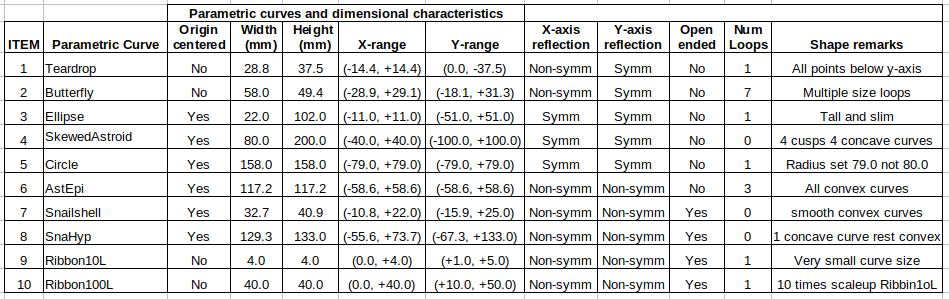
\includegraphics[width=1.70\textwidth]{Images/Chap3/Parametric-Curve-shapes-and-dimensions.png} 
	\end{figure}	
\end{landscape}

%% ===============================================
\clearpage
\pagebreak

\section{Links to parametric curves}

\noindent
The following links will jump directly to the figures and their parametric equations.

\begin{enumerate}
	\item Teardrop curve Fig [\ref{Teardrop-curve-plot-BW.pdf}]
	
	\item Teardrop comparison: Zhong et. al.(2018) Fig [\ref{Comparison-Teardrop-Zhong-et-al-2018.png}]
	
	\item Butterfly curve Fig [\ref{Butterfly-curve-plot-BW.pdf}]
	
	\item Butterfly NURBS comparison: Ni et. al.(2018) Fig [\ref{Comparison-Butterfly-Ni-et-al(2018)}]
	
	\item Butterfly NURBS comparison: Hu et. al.(2023) Fig [\ref{Comparison-Butterfly-Hu-et-al(2023)}]
	
	\item Ellipse curve Fig [\ref{Ellipse-curve-plot-BW.pdf}]
	
	\item SkewedAstroid curve Fig [\ref{SkewedAstroid-curve-plot-BW.pdf}]
	
	\item Circle Fig [\ref{Circle-curve-plot-BW.pdf}]
	
	\item AstEpi curve Fig [\ref{AstEpi-curve-plot-BW.pdf}]
	
	\item Snailshell curve Fig [\ref{Snailshell-curve-plot-BW.pdf}]
	
	\item SnaHyp curve Fig [\ref{SnaHyp-curve-plot-BW.pdf}]
	
	\item Ribbon10L curve Fig [\ref{Ribbon10L-curve-plot-BW.pdf}]
	
	\item Ribbon100L curve Fig [\ref{Ribbon100L-curve-plot-BW.pdf}]
	
	\item Ribbon B-Splines comparison: Zhong-et-al(2018) Fig [\ref{Comparison-Ribbon-Zhong-et-al(2018)}]
	
	
\end{enumerate}



%% ===============================================
\clearpage
\pagebreak

\begin{figure}
	\caption{Teardrop shape profile}
	\label{Teardrop-curve-plot-BW.pdf}
	\centering
	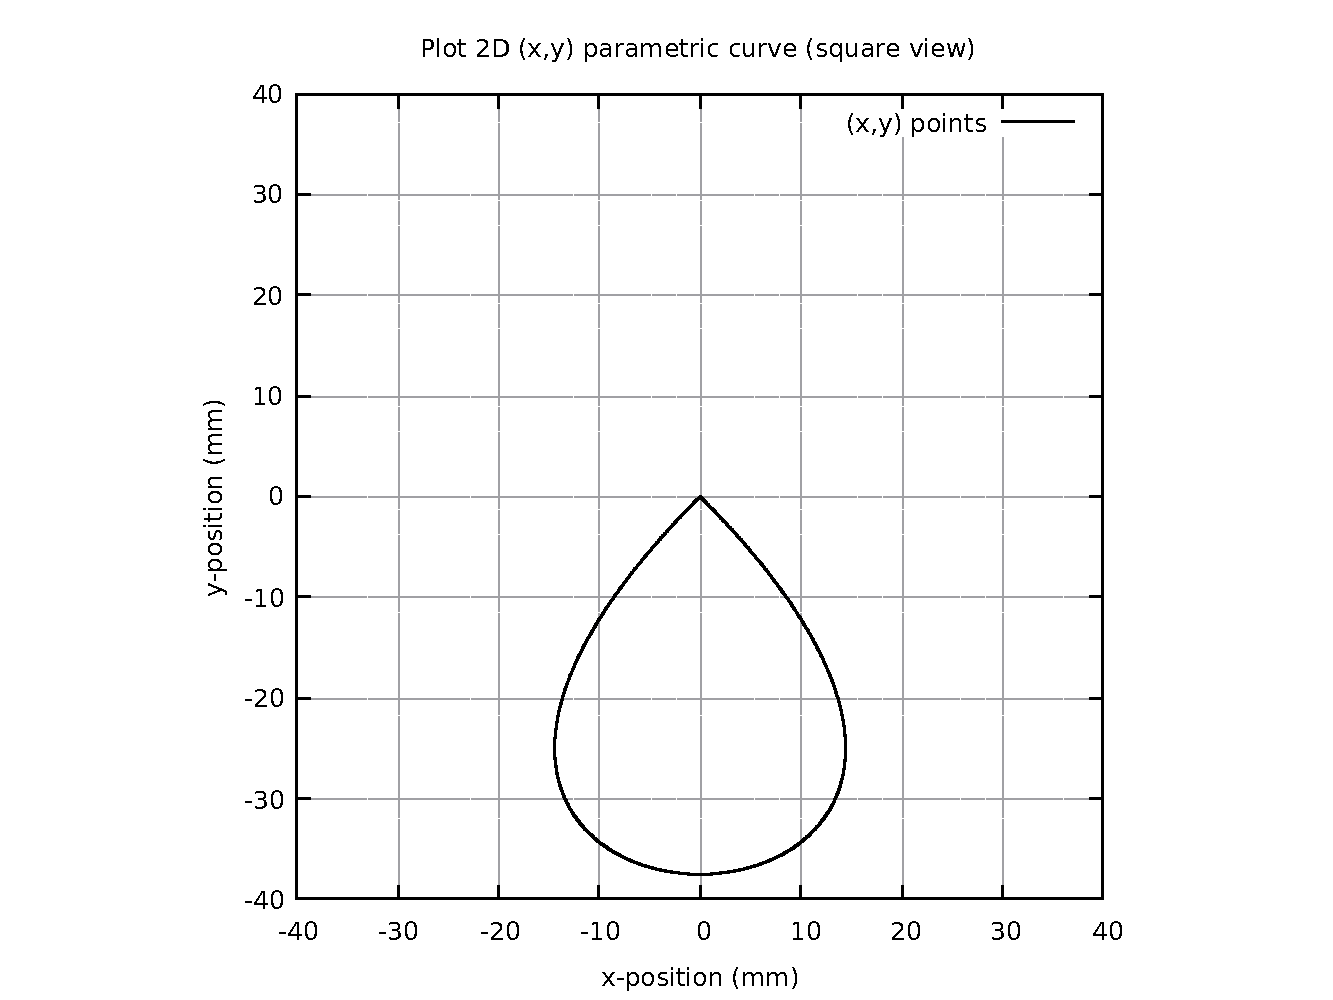
\includegraphics[width=1.00\textwidth]{Chap3/curve-shape/curves/Teardrop-curve-plot-BW.pdf} 
\end{figure}

\begin{table}[ht]
	\begin{center}
		\begin{tabular}{ p{16.0cm} }
			\caption{Teardrop curve parametric equation}
			\begin{eqnarray}
				x(u) & = & - 150u + 450u^2 - 300u^3 \nonumber \\   
				y(u) & = & - 150u + 150u^2 \nonumber \\
				u & \in & [0.0, 1.0] \nonumber
			\end{eqnarray}
		\end{tabular}
	\end{center}
\end{table}

%% TEARDROP ZHONG COMPARISONS
%% ====================
\clearpage
\pagebreak

\begin{figure}
	\caption{Teardrop comparison Zhong et. al. (2018) }
	\label{Comparison-Teardrop-Zhong-et-al-2018.png}
	\centering
	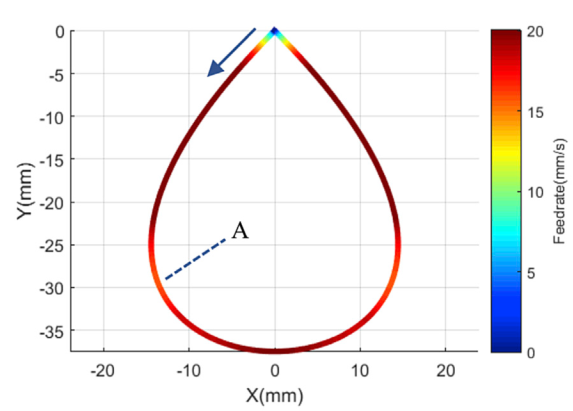
\includegraphics[width=0.750\textwidth]{Images/Chap3/Comparison-Teardrop-Zhong-et-al-2018.png} 
\end{figure}

This figure by Zhong et. al. (2018) above is identical to the one used in this work because the same parametric equation was used. Even though the interpolation method is different, the results are similar but not identical. The flowchart in their work is complex and complicated to understand. As a comparison, the flowchart and algorithm in this work is simpler, and computations are fully functionalized and modularized.\\

Notice that this Teardrop figure by Zhong et. al. (2018) above is plotted on a rectangular grid (x and y intervals are not the same size), instead of a square grid done in this work shown in Fig [\ref{Teardrop-curve-plot-BW.pdf}]. This rectangular grid gives a false impression of a wider bottom for the Teardrop, that actually is not the case.\\ 

In addition, the Teardrop figure by Zhong is not presented in an overall grid that is square and origin-centered. It does not provide information on the placement of the Teardrop location relative to the origin. This origin-centered presentation provides information regarding the x and y axes reflection symmetry for the particular curve. \\



%% BUTTERFLY CURVE EQUATION
%% ====================
\clearpage
\pagebreak

\begin{figure}
	\caption{Butterfly shape profile}
	\label{Butterfly-curve-plot-BW.pdf}
	\centering
	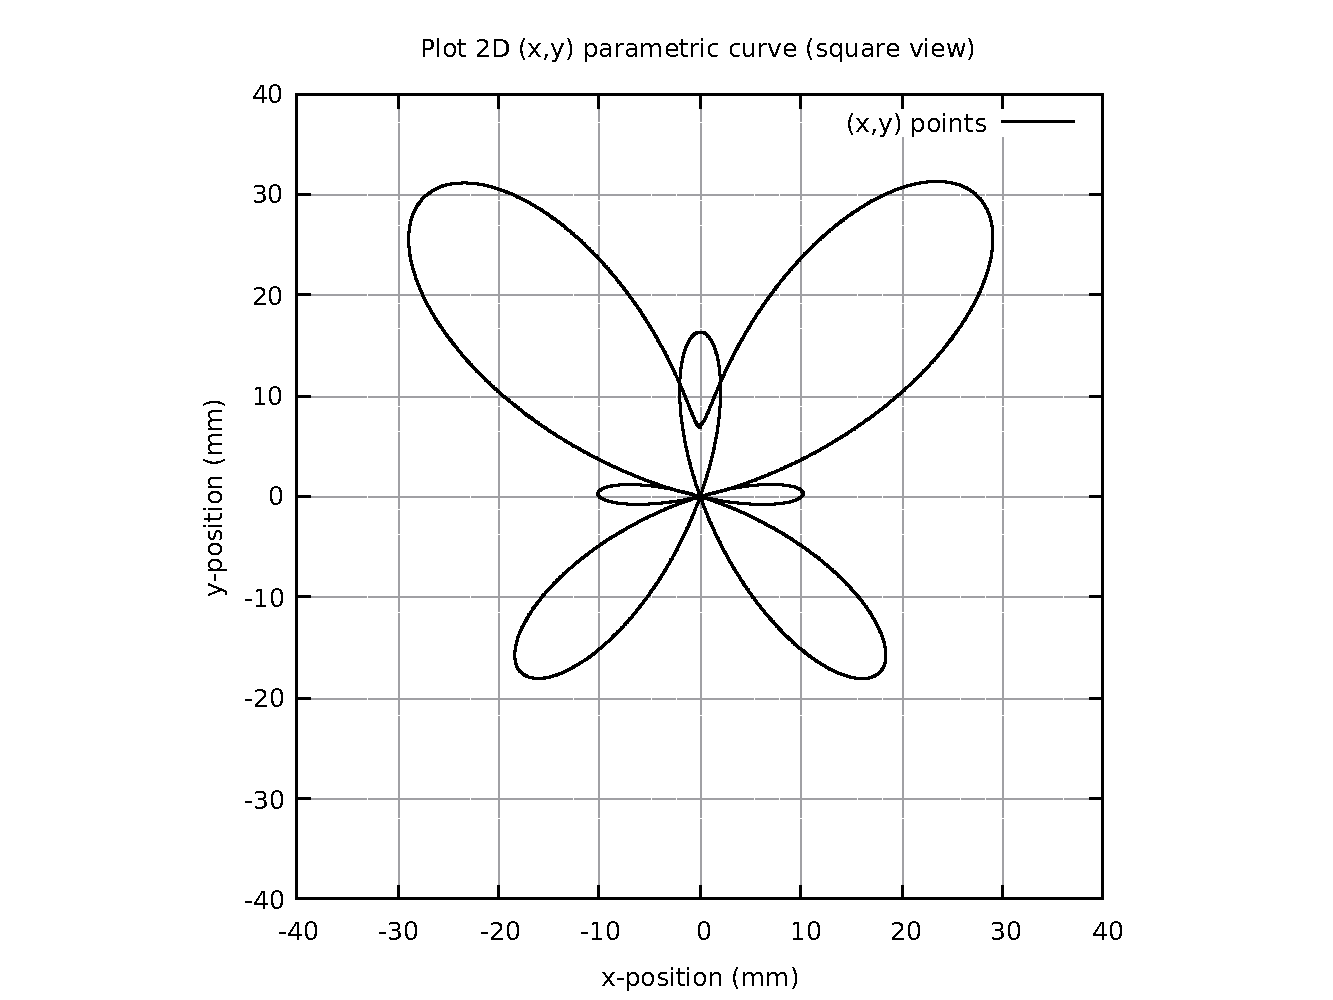
\includegraphics[width=1.00\textwidth]{Chap3/curve-shape/curves/Butterfly-curve-plot-BW.pdf} 
\end{figure}

\begin{table}[ht]
\begin{center}
\begin{tabular}{ p{16.0cm} }
\caption{Butterfly curve parametric equation}
\begin{eqnarray}
	x(u) & = & \sin(2\pi u) \left [ e^{\cos(2\pi u)} - 2\cos(8\pi u) - (\sin(2\pi u/12))^5 \right] \nonumber \\
	y(u) & = & \cos(2\pi u) \left [ e^{\cos(2\pi u)} - 2\cos(8\pi u) - (\sin(2\pi u/12))^5 \right] \nonumber \\
	u & \in & [0.0, 1.0] \nonumber
\end{eqnarray}
\end{tabular}
\end{center}
\end{table}


%% ==========================================
\clearpage
\pagebreak

%% BUTTERFLY COMPARISON 1
\begin{figure}
	\caption{Butterfly comparison Ni et. al. (2018) NURBS}
	\label{Comparison-Butterfly-Ni-et-al(2018)}
	\centering
	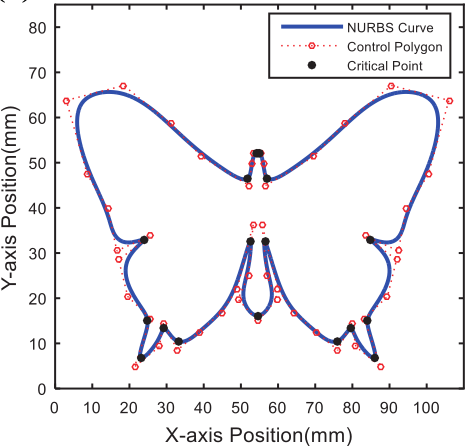
\includegraphics[width=0.70\textwidth]{Images/Chap3/Comparison-Butterfly-Ni-et-al-2018.png} 
\end{figure}

%% BUTTERFLY COMPARISON 2
\begin{figure}
	\caption{Butterfly comparison Hu et. al. (2023) NURBS }
	\label{Comparison-Butterfly-Hu-et-al(2023)}
	\centering
	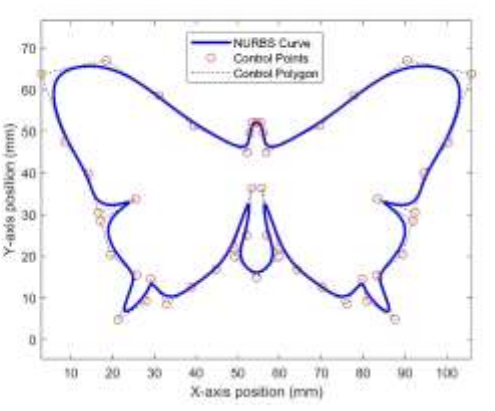
\includegraphics[width=0.78\textwidth]{Images/Chap3/Comparison-Butterfly-Hu-et-al-2023.png} 
\end{figure}

%% \noindent Note: The original is not clear.
%% ============================================

%% ELLIPSE CURVE EQUATION
%% ====================
\clearpage
\pagebreak

\begin{figure}
	\caption{Ellipse shape profile}
	\label{Ellipse-curve-plot-BW.pdf}
	\centering
	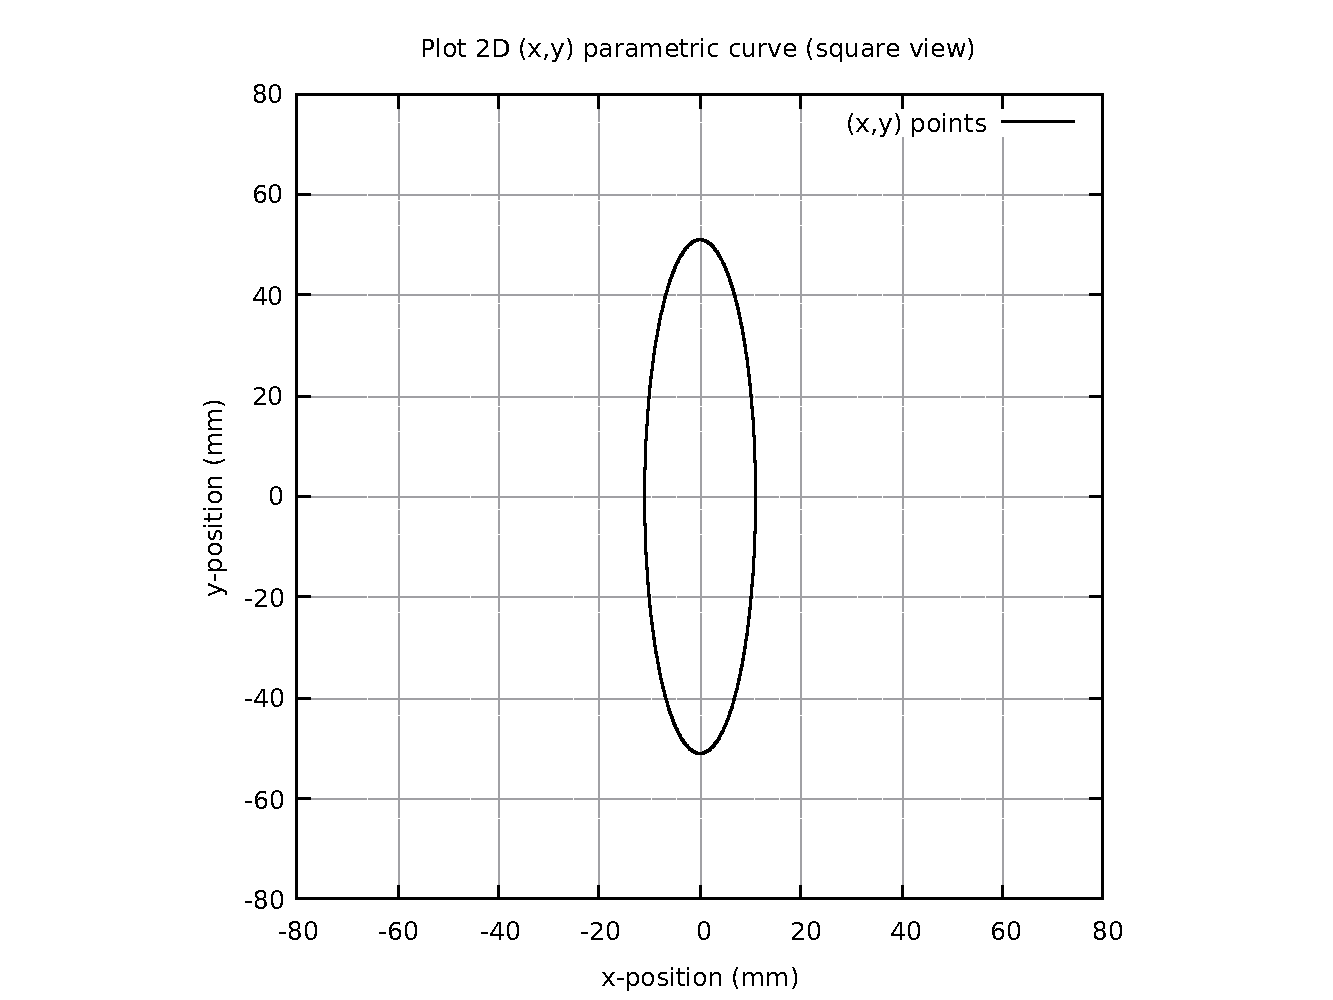
\includegraphics[width=1.20\textwidth]{Chap3/curve-shape/curves/Ellipse-curve-plot-BW.pdf} 
\end{figure}

\begin{table}[ht]
\begin{center}
\begin{tabular}{ p{16.0cm} }
\caption{Ellipse curve parametric equation}
\begin{eqnarray}
	x(u) & = & 11\sin(2\pi u) \nonumber \\   
	y(u) & = & 51\cos(2\pi u) \nonumber \\
	& \in & [0.0, 1.0] \nonumber
\end{eqnarray}
\end{tabular}
\end{center}
\end{table}


%% SKEWEDASTROID CURVE EQUATION
%% ====================
\clearpage
\pagebreak

\begin{figure}
	\caption{SkewedAstroid shape profile}
	\label{SkewedAstroid-curve-plot-BW.pdf}
	\centering
	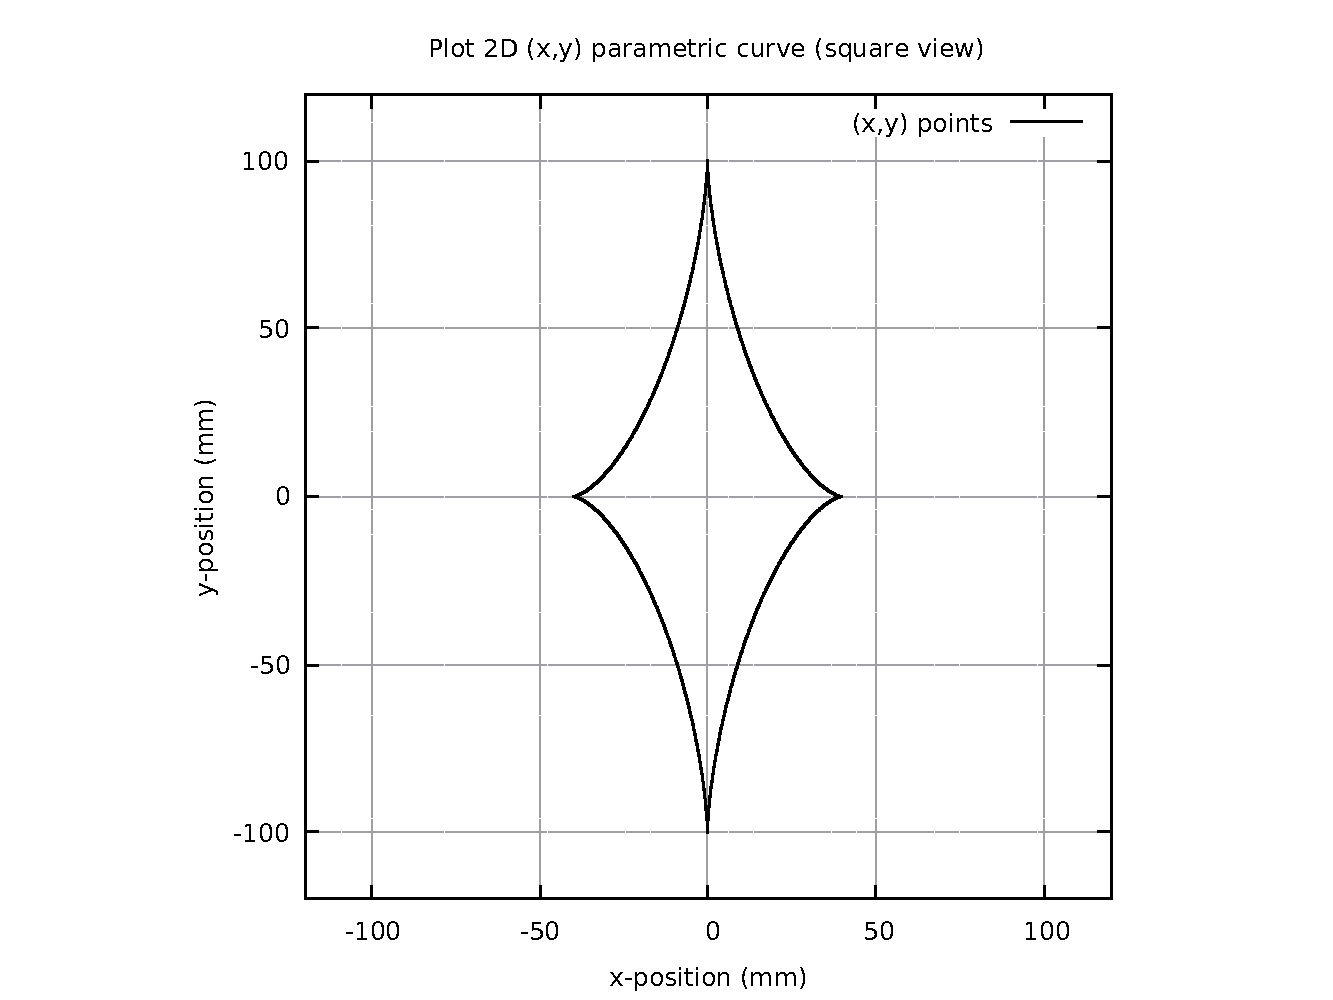
\includegraphics[width=1.20\textwidth]{Chap3/curve-shape/curves/SkewedAstroid-curve-plot-BW.pdf} 
\end{figure}

\begin{table}[ht]
\begin{center}
\begin{tabular}{ p{16.0cm} }
\caption{SkewedAstroid curve parametric equation}
\begin{eqnarray}
	x(u) & = & 40  [ \sin(2\pi u) ]^3  \nonumber \\
	y(u) & = & 100 [ \cos(2\pi u) ]^3  \nonumber \\
	u & \in & [0.0, 1.0] \nonumber
\end{eqnarray}
\end{tabular}
\end{center}
\end{table}

%% CIRCLE
%% ==================================================
\clearpage
\pagebreak

\begin{figure}
	\caption{Circle shape profile}
	\label{Circle-curve-plot-BW.pdf}
	\centering
	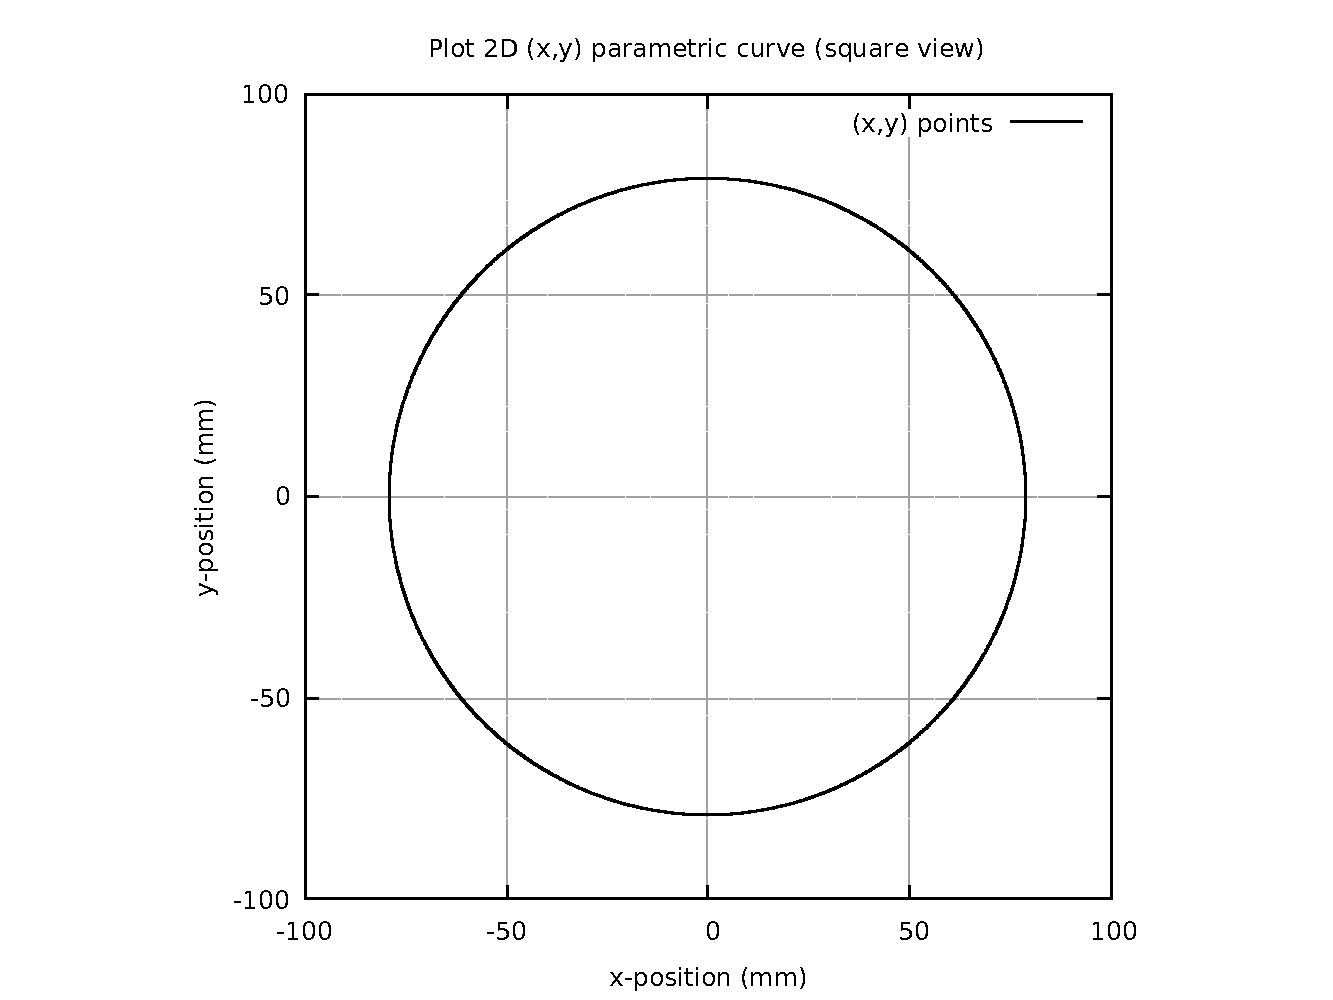
\includegraphics[width=1.20\textwidth]{Chap3/curve-shape/curves/Circle-curve-plot-BW.pdf} 
\end{figure}

\begin{table}[ht]
\begin{center}
\begin{tabular}{ p{16.0cm} }
\caption{Circle parametric equation}
\begin{eqnarray}
	x(u) & = & 79\sin(2\pi u) \nonumber \\   
	y(u) & = & 79\cos(2\pi u) \nonumber \\
	u & \in & [0.0, 1.0] \nonumber
\end{eqnarray}
\end{tabular}
\end{center}
\end{table}

%% ASTEPI 
%% ==================================================
\clearpage
\pagebreak

\begin{figure}
	\caption{AstEpi shape profile}
	\label{AstEpi-curve-plot-BW.pdf}
	\centering
	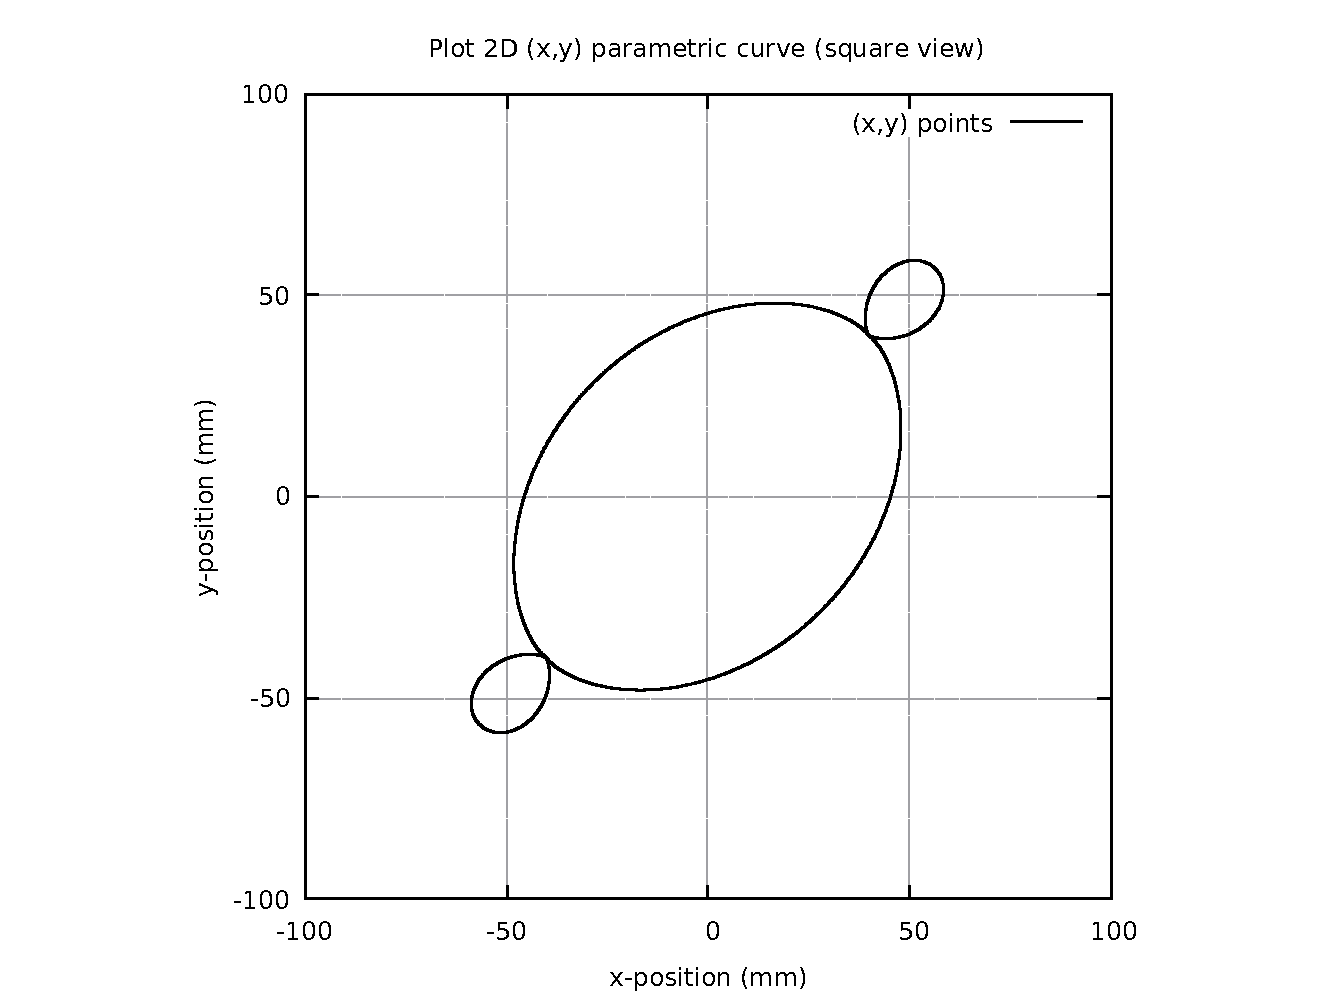
\includegraphics[width=1.20\textwidth]{Chap3/curve-shape/curves/AstEpi-curve-plot-BW.pdf} 
\end{figure}


\begin{table}[ht]
\begin{center}
\begin{tabular}{ p{16.0cm} }
\caption{AstEpi curve parametric equation}
\begin{eqnarray}
	tvtiny & = & 0.0000000001 \nonumber \\
	x(u) & = & 40[\sin(2\pi u)]^3 + 50\cos(2\pi u + tvtiny) - 10\cos(10\pi u -tvtiny) \nonumber \\
	y(u) & = & 40[\cos(2\pi u)]^3 + 50\sin(2\pi u + tvtiny) - 10\sin(10\pi u -tvtiny) \nonumber \\
	u & \in & [0.0, 1.0] \nonumber
\end{eqnarray}
\end{tabular}
\end{center}
\end{table}

%% SNAILSHELL
%% ==================================================
\clearpage
\pagebreak

\begin{figure}
	\caption{Snailshell shape profile}
	\label{Snailshell-curve-plot-BW.pdf}
	\centering
	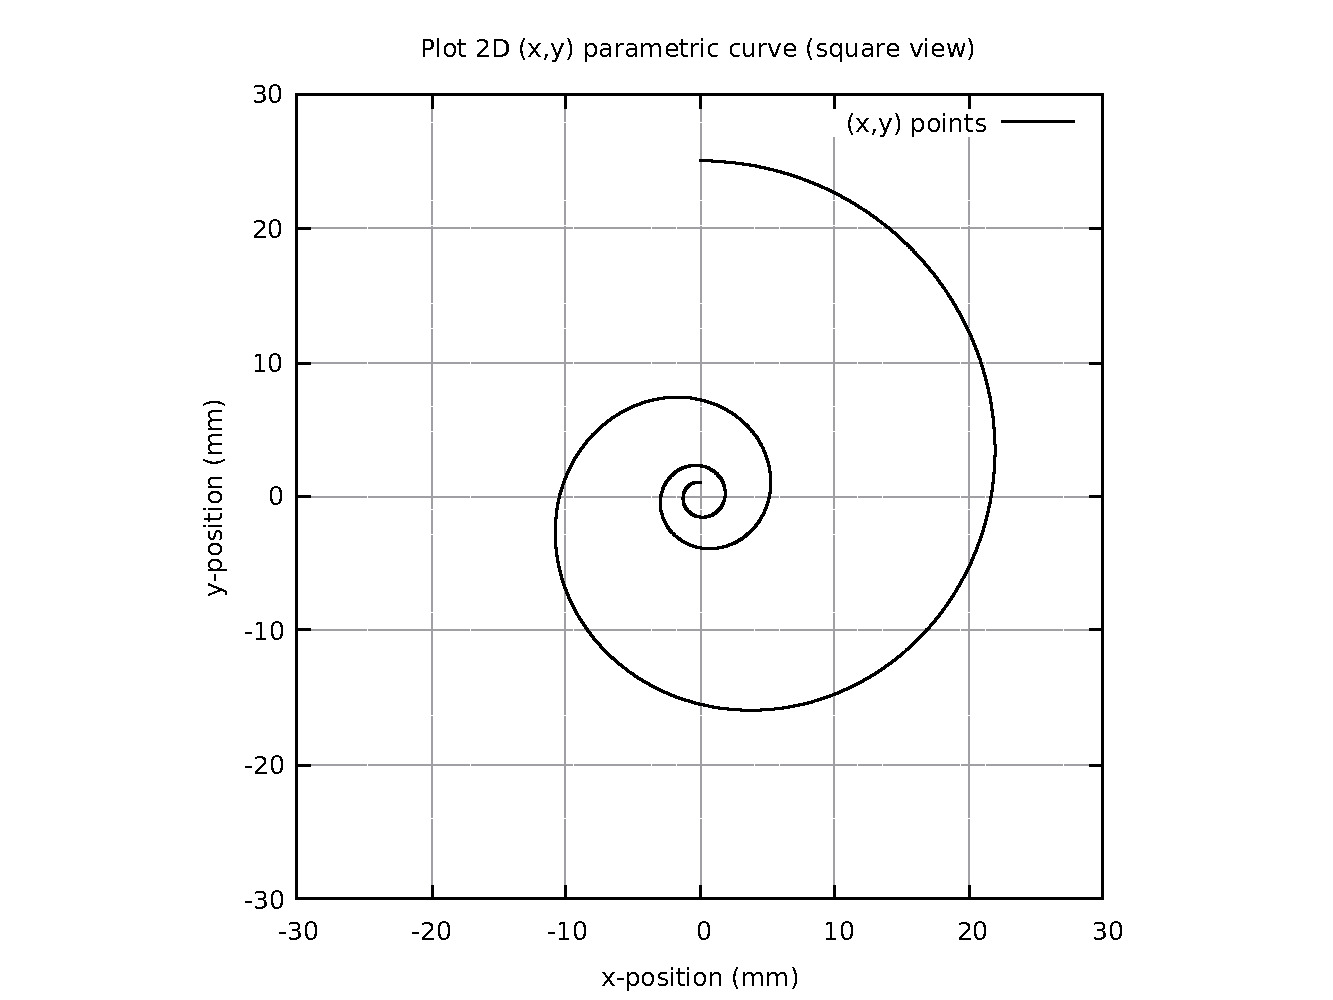
\includegraphics[width=1.20\textwidth]{Chap3/curve-shape/curves/Snailshell-curve-plot-BW.pdf} 
\end{figure}


\begin{table}[ht]
\begin{center}
\begin{tabular}{ p{16.0cm} }
\caption{Snailshell curve parametric equation}
\begin{eqnarray}
	x(u) & = & 100\sin(6\pi u) / [9 (\pi u)^2 + 4] \nonumber \\   
	y(u) & = & 100\cos(6\pi u) / [9 (\pi u)^2 + 4] \nonumber \\
	u & \in & [0.0, 1.0] \nonumber
\end{eqnarray}
\end{tabular}
\end{center}
\end{table}


%% SNAHYP
%% ==================================================
\clearpage
\pagebreak

\begin{figure}
	\caption{SnaHyp shape profile}
	\label{SnaHyp-curve-plot-BW.pdf}
	\centering
	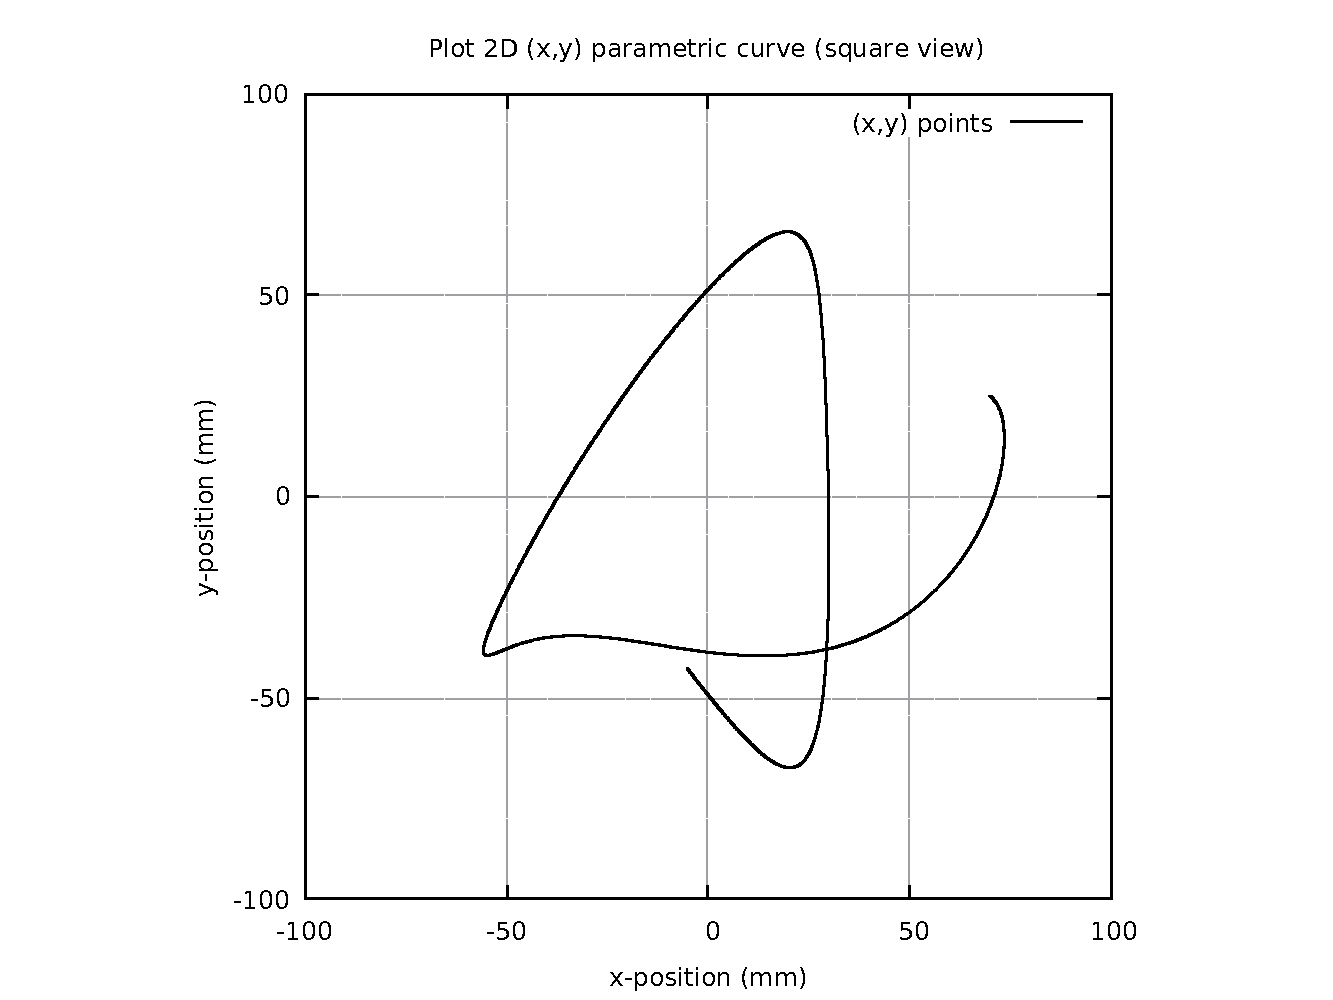
\includegraphics[width=1.20\textwidth]{Chap3/curve-shape/curves/SnaHyp-curve-plot-BW.pdf} 
\end{figure}

\begin{table}[ht]
\begin{center}
\begin{tabular}{ p{16.0cm} }
\caption{SnaHyp curve parametric equation}
\begin{eqnarray}
	xsna(u) & = & [4\sin(8\pi u) ] / [16 (\pi u)^2 + 4] \nonumber \\
	xhyp(u) & = & [2\cos(4\pi u)  + 5\cos(8\pi u /3)  ] \nonumber \\
	x(u) & = & 10[xsna(u) + xhyp(u)] \nonumber \\
	ysna(u) & = & [10\cos(8\pi u)] / [16 (\pi u)^2 + 4] \nonumber \\
	yhyp(u) & = & [2\sin(8\pi u) - 5\sin(8\pi u /3)] \nonumber \\
	y(u) & = & 10[ysna(u) + yhyp(u)] \nonumber \\
	u & \in & [0.0, 1.0] \nonumber
\end{eqnarray}
\end{tabular}
\end{center}
\end{table}

%% RIBBON10L
%% ==================================================
\clearpage
\pagebreak

\begin{figure}
	\caption{Ribbon10L shape profile}
	\label{Ribbon10L-curve-plot-BW.pdf}
	\centering
	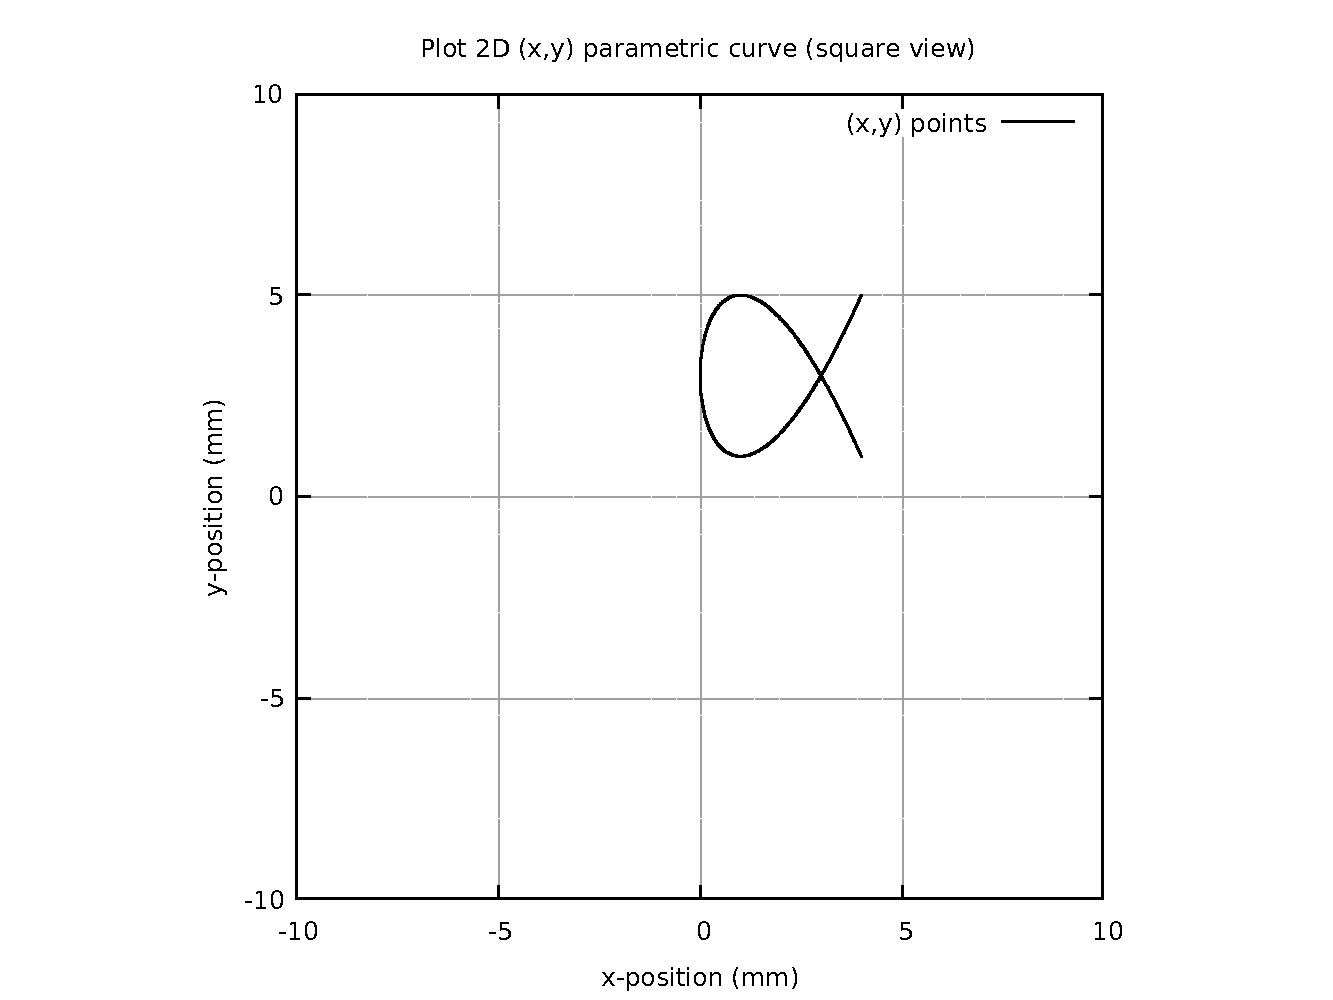
\includegraphics[width=1.20\textwidth]{Chap3/curve-shape/curves/Ribbon10L-curve-plot-BW.pdf} 
\end{figure}

\begin{table}[ht]
\begin{center}
\begin{tabular}{ p{16.0cm} }
\caption{Ribbon10L curve parametric equation}
\begin{eqnarray}
	t(u) & = & 4(u - 0.50) \nonumber \\
	x(u) & = & t^2 \nonumber \\   
	y(u) & = & t^3 - 3t + 3 \nonumber \\
	u & \in & [0.0, 1.0] \nonumber
\end{eqnarray}
\end{tabular}
\end{center}
\end{table}

%% Ribbon100L
%% ==================================================
\clearpage
\pagebreak

\begin{figure}
	\caption{Ribbon100L shape profile}
	\label{Ribbon100L-curve-plot-BW.pdf}
	\centering
	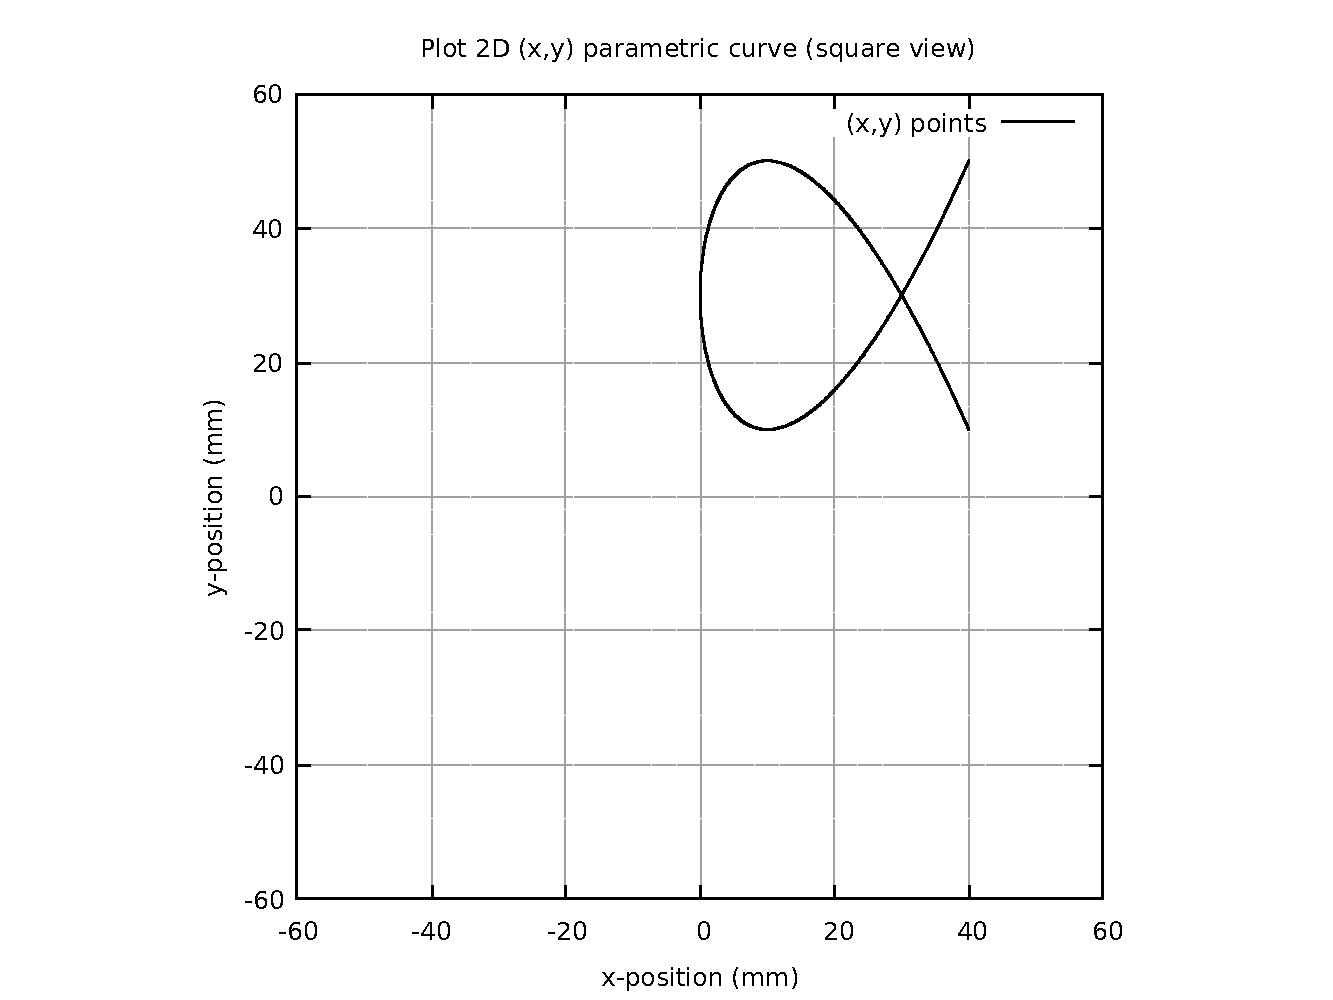
\includegraphics[width=1.20\textwidth]{Chap3/curve-shape/curves/Ribbon100L-curve-plot-BW.pdf} 
\end{figure}

\begin{table}[ht]
\begin{center}
\begin{tabular}{ p{16.0cm} }
\caption{Ribbon100L curve parametric equation}
\begin{eqnarray}
	t(u) & = & 4(u - 0.50) \nonumber \\
	x(u) & = & 10t^2 \nonumber \\   
	y(u) & = & 10t^3 - 30t + 30 \nonumber \\
	u & \in & [0.0, 1.0] \nonumber
\end{eqnarray}
\end{tabular}
\end{center}
\end{table}


%% RIBBON ZHONG COMPARISONS
%% ====================
\clearpage
\pagebreak

\begin{figure}
	\caption{Ribbon comparison Zhong et. al. (2018) B-Splines}
	\label{Comparison-Ribbon-Zhong-et-al(2018)}
	\centering 
	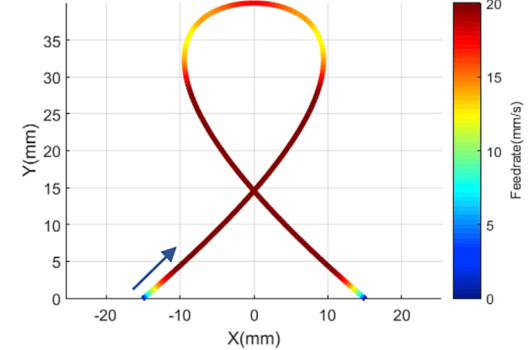
\includegraphics[width=0.80\textwidth]{Images/Chap3/Comparison-Ribbon-Zhong-et-al-2018.png} 
\end{figure}

Compared to this work which uses the standard third degree polynomial for the Ribbon curve, the representation by \cite{Zhong-etal:2018} is a NURBS type, 3rd degree B-Spline with control points\\

$\{P_{i}\} = \{ (-15,0), (20,30), (0,50), (-20,30), (15,0)  \}$ \\
and knot vectors $U = \{0, 0, 0, 0, 0.5, 1, 1, 1, 1\}$.\\

NURBS or Non-Uniform Rational B-Splines are a generalization of B-Splines. Note that NURBS can create smooth and precise shapes that can be scaled, rotated, and deformed without losing quality. Splines are simpler curves that are defined by a set of control points and a degree of smoothness.\\



%% ==================================
\clearpage
\pagebreak

\section{Direction of travel in parametric curves}

With a 3D plot of the Teardrop curve, direction of traversal of the $u$ point can be easily visualized. It begins from $u=0$ to $u=1$. Upon collapsing the $u(t)$ axis, it becomes a 2D Teardrop closed curve again. This means parametric interpolations provide direction of traversal for curves and surfaces through the parameter $u(t)$. \\

\begin{figure}
	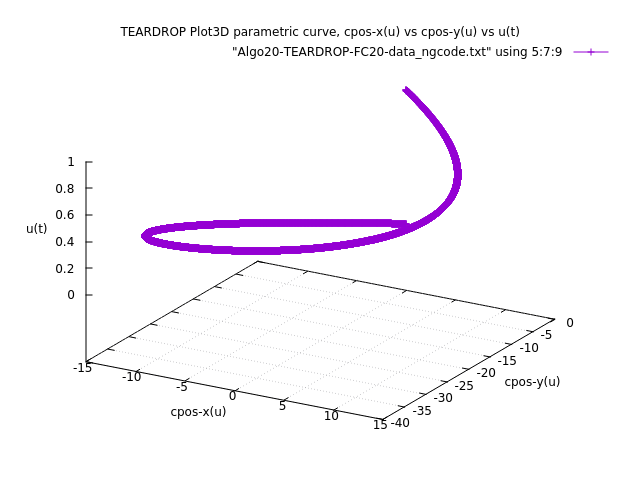
\includegraphics[width=1.10\textwidth]{Chap4/images/TEARDROP-plot-3D-x-vs-y-vs-u.png} 
	\label{TEARDROP-plot3D-data_ngcode.png}
	\caption{Teardrop 3D plot x(u) vs y(u) vs u(t)}
\end{figure}

\clearpage
\pagebreak

\begin{figure}
	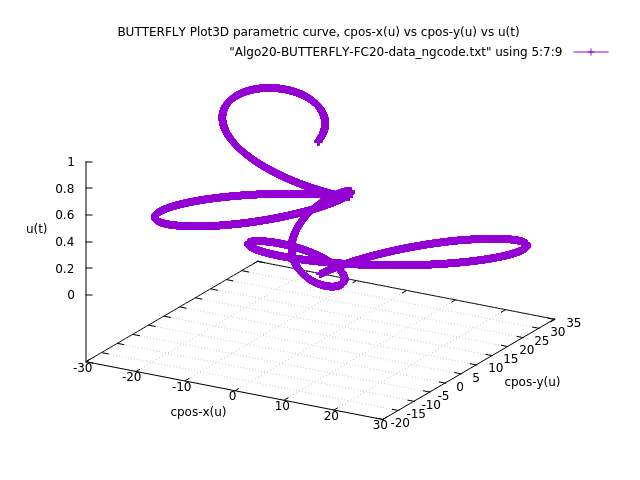
\includegraphics[width=1.10\textwidth]{Chap4/images/BUTTERFLY-plot-3D-x-vs-y-vs-u.png} 
	\label{BUTTERFLY-plot3D-data_ngcode.png}
	\caption{Butterfly 3D plot x(u) vs y(u) vs u(t)}
\end{figure}


The 3D plot for the Butterfly looks messy but the principle is the same. When the $u(t)$ axis collapses, it becomes a 2D Butterfly closed curve again.


%% ==================================================
%% ==================================================
\clearpage
\pagebreak

\section{Chord-error concept}

\begin{figure}
	\caption{Chord-error eps ($\epsilon$), Feedrate F, and Interpolation time T}
	\label{Chord-error-image.png}
	\centering
	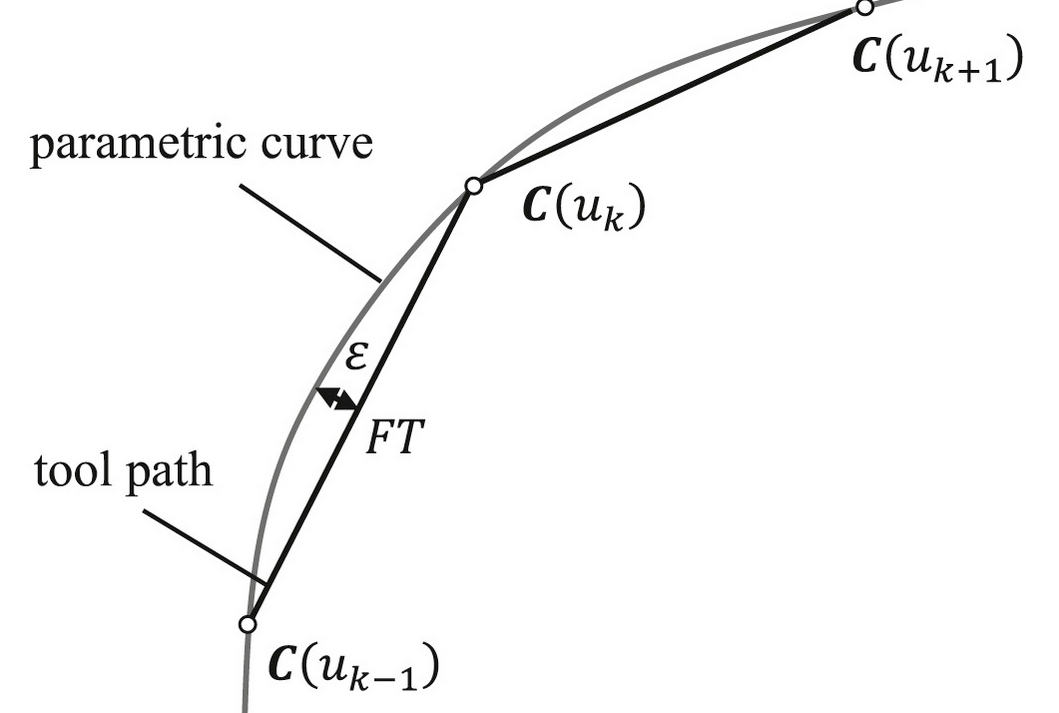
\includegraphics[width=0.80\textwidth]{Images/Chap3/Chord-error-image.png} 


\end{figure}

The relationship between the parametric curve, chord-error and machine feedrate is illustrated in the Fig [\ref{Chord-error-image.png}] above. (Source: \cite{Zhong-etal:2018}) It shows 3 successive interpolated points $C(u_{k-1})$, $C(u_{k})$ and $C(u_{k+1})$ as the parameter is incremented from $u_{k-1}$ to  $u_{k}$ and  $u_{k+1}$ along the parametric curve. \\

The chord is defined as the line connecting two points on the parametric curve. The chord-error $\epsilon$ is the maximum distance of a line from the curve perpendicular to the chord. If F is the feedrate (mm/s) and T is the interpolation period (s), that is, time duration to move from one point to the next, then the product of feedrate with interpolation time gives the length of the chord (FT).\\

The calculation method for the chord-error ($\epsilon$) between two points on the parametric curve is described in section Chord-error $eps(u)$ [\ref{chap3-Chord-error eps}].

\section{Chord-error minimization}

A decrease in the chord length (FT), will cause a decrease the chord-error ($\epsilon$). This is favorable for accuracy since the toolpath follows closer to the path trajectory of the parametric curve. However, decreasing the chord-length causes an increase in the number of interpolated points for the same length of the curve. Since the interpolation time for a single step is a constant, this will also increase the total machining time, a feature that is not favorable. 
 
\section{Feedrate maximization}

An increase in feedrate (F) of the CNC machining tool, will decrease the total machining time. This is favourable for faster completion of machining for the same length of the curve. However, the increase in feedrate will cause a larger chord length (FT), thus a larger chord-error ($\epsilon$).

\section{Chord-error and feedrate constraints}

The approach in this work is to establish a combined chord-error and feedrate constraint. It is based on the following:

\begin{enumerate}
	\item A strict maximum chord-error value is set as the error-tolerance. Every move in the interpolated point-to-point traversal must not exceed this error-tolerance. 
	
	\item Every move in the interpolated point-to-point traversal must not exceed the calculated feedrate limit for that particular point.

    \item The feedrate limit at any particular point is calculated based on a combined geometric, dynamic and kinematic factors of the particular CNC machine. 
	
\end{enumerate}

\section{Brief on algorithm strategy and design}

In This-Work, the realtime parametric curve algorithm will be designed to iterate every point-to-point, as step move, such that the chord-error is below error-tolerance and the current feedrate is close but below the feedrate limit, that is, before the next move is taken. This is the criteria of iterative convergence. The cycle repeats until the point-to-point traversal of the entire parametric curve is completed.\\

Without exception, the flowcharts in This-Work are all of the type, "one way in and one way out". This strategy or paradigm is called "structured programming". Every functional computation unit implemented in this realtime interpolation algorithm comply with this structured programming strategy. In addition, various reports were generated, written to text files,  to capture every variable change and transaction during the execution of the algorithm. This facilitates very easy search, analysis and debugging. \\

About structured programming algorithms, the following two(2) figures in the next section are basic examples of structured programming algorithms. Fig[\ref{img-Example-1-Structured Programming Design}] and Fig[\ref{img-Example-2-Structured Programming Design}] show the basic sequence and iterative loop. Both examples exhibit features of program flows in a "one way in and one way out" pattern. \\

About non-structured programming algorithms, the next two(2) figures demonstrate its features. The program flow in this case is difficult to track and so not easy to comprehend. Fig[\ref{img-Example-3-Non-Structured Programming Design}] shows overlapping flows in functional units "B" and "X" nodes, while Fig[\ref{img-Example-4-Non-Structured Programming Design}], is considered non-structured programming because there is "one-way-in but four-ways-out". \\	

%% ==================================================
\clearpage
\pagebreak

\begin{figure}
	\centering
	\caption  {Example-1-Structured Programming Design (1-in, 1-out)}
	\label{img-Example-1-Structured Programming Design}
	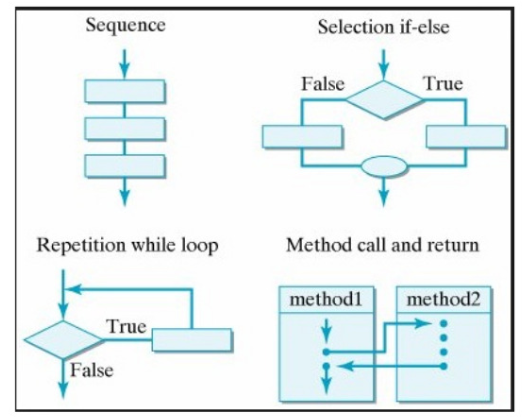
\includegraphics[width= 0.80\textwidth]{Chap3/AlgorithmTypes/Example-1-Structured-Programming-design.png} 
\end{figure}		


\begin{figure}
	\centering
	\caption  {Example-2-Structured Programming Design (1-in, 1-out)}
	\label{img-Example-2-Structured Programming Design}
	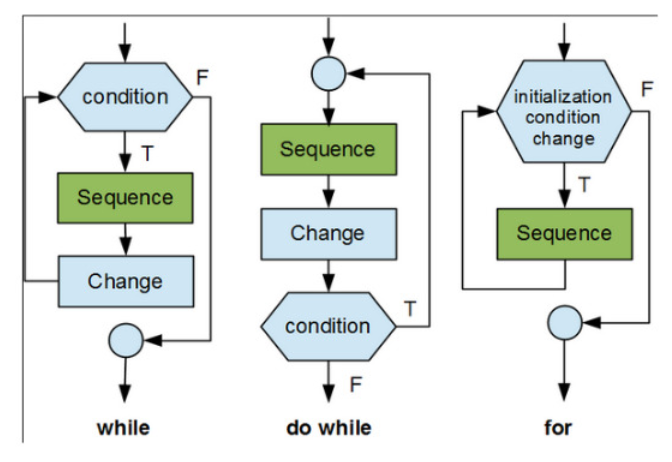
\includegraphics[width= 0.80\textwidth]{Chap3/AlgorithmTypes/Example-2-Structured-Programming-design.png} 
\end{figure}		

%% =======================================================
\clearpage
\pagebreak

\begin{figure}
	\centering
	\caption  {Example-3-Non-Structured Programming Design, (S=Start, E=Exit)}
	\label{img-Example-3-Non-Structured Programming Design}
	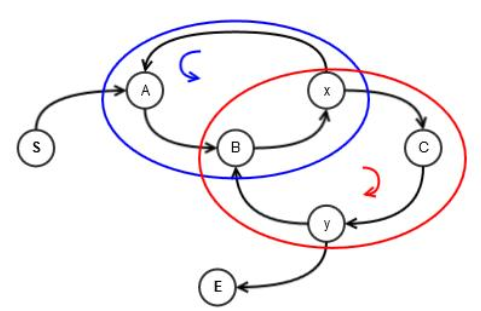
\includegraphics[width= 0.70\textwidth]{Chap3/AlgorithmTypes/Example-3-Non-Structured-Programming-design.png} 
\end{figure}		



\begin{figure}
	\centering
	\caption  {Example-4-Non-Structured Programming Design (1-in, 4-outs)}
	\label{img-Example-4-Non-Structured Programming Design}
	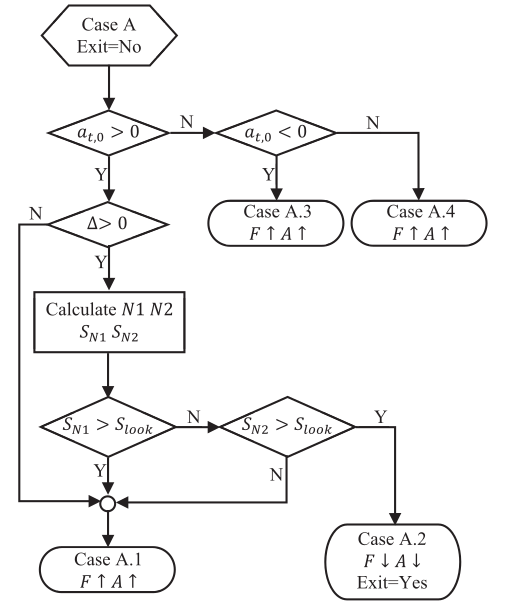
\includegraphics[width= 0.60\textwidth]{Chap3/AlgorithmTypes/Example-4-Non-Structured-Programming-design.png} 
\end{figure}		



%% ==================================================
\clearpage
\pagebreak

\section{Radius of Curvature $\textbf{rho(u)}$}

The radius of curvature ($R$ or $rho$) is important in inspection of curves and surfaces. The value of $rho$ is the reciprocal of curvature, $K$. So $rho = (1/K)$. For a curve, $rho(u)$ equals the radius of circular arc which best approximates the curve at that point $u$. The curvature $K$, is the amount by which a curve deviates from being a straight line, or a surface deviates from being a plane (not flat).\\

Note that the radius of curvature $rho(u)$ is constant for a circle over all applicable values of parameter $u$. Essentially, the value of $rho(u)$ is just the radius of the circle itself. \\ 

Consider a series of concentric circles with the radii increasing from zero to some large number. Intuitively, an increasing $rho(u)$ value means the curvature opens to a larger and larger circle radius. On the contrary, a decreasing $rho(u)$ value means the curvature closes to a smaller and smaller circle radius. 


%% \clearpage
%% \pagebreak


When $rho(u)$ becomes zero, the curve shrinks to a single point and there is no curvature or curving behaviour. When $rho(u)$ value reaches infinity, it becomes a straight line and there is also no curving behaviour. This is an important general rule when visually inspecting curves and surfaces.\\

If the curve is given parametrically by functions $x(u)$ and $y(u)$, then from standard calculus and analytic geometry, the exact derivation for radius of curvature is given by:

\[ R(u) = rho(u) = \Bigg | \frac{numerator(u)}{denominator(u)} \Bigg |  \]
\[ K(u) = curvature(u) =  \Bigg | \frac{denominator(u)}{numerator(u)} \Bigg |  \]
where 
\[ numerator(u) = \Bigg ( \Bigg ({\odv{x(u)}{u}} \Bigg )^{2} + \Bigg ({\odv{y(u)}{u}}\Bigg )^{2} \Bigg ) ^{3/2}  \]
\[ denominator(u) = \Bigg(\odv{x(u)}{u}\Bigg)\Bigg(\frac{\mathrm{d^2}y(u)}{\mathrm{d}u^2}\Bigg) - \Bigg(\frac{\mathrm{d^2}x(u)}{\mathrm{d}u^2}\Bigg)\Bigg(\odv{y(u)}{u}\Bigg)  \]


%% $
%% \frac{\mathrm{d^2}y(u)}{\mathrm{d}u^2} 
%%
%% \frac{\mathrm{d^2}x(u)}{\mathrm{d}u^2}
%% $ 


% ================================
%% \clearpage
%% \pagebreak

\section{Chord-error $\textbf{eps(u)}$}
\label{chap3-Chord-error eps}

The chord-error (epsilon) is the maximum length of the line perpendicular to the chord from a point on the arc segment. Based on extensive computer simulations, it was found that the perpendicular line starting from the mid-point on the chord that intersects the arc segment gives the maximum length. The algorithm for calculating $eps(u)$ is as follows:

\begin{enumerate}
	\item From the current u-point giving an $C(x(u), y(u))$ point on the parametric curve, determine the $C(x(u+next), y(u+next))$ point value on the curve. This is just the next interpolated point on the curve. 
	
	\item Construct a chord line between the points $C(x(u), y(u))$ and $C(x(u+next), y(u+next))$. Calculate the slope of this chord line. Call it $chordslope$.
	
	\item From geometry, any line that is perpendicular to this chord will have a slope of $perplineslope = (-1/chordslope)$.
	
	\item Find the mid-point coordinates $x_{mid}$ and $y_{mid}$ on this chord line.
	
	\item From the known $chordslope$ and chord mid-point coordinates, generate a linear equation perpendicular to this line. Call it the $perpline$.
	
	\item Find the intersection coordinates of the given parametric curve (arc segment) with the $perpline$. Call these coordinates $x_{int}$ and $y_{int}$. 
	
	\item The calculated value of chord-error $eps(u)$ is the linear length between the points ($x_{mid}$,$y_{mid}$) and ($x_{int}$ and $y_{int}$).
	
	\item The linear length is calculated using the standard Pythagoras formula in Cartesian coordinates.
	
\end{enumerate}

% ================================
%% \clearpage
%% \pagebreak
\begin{figure}
	\centering
	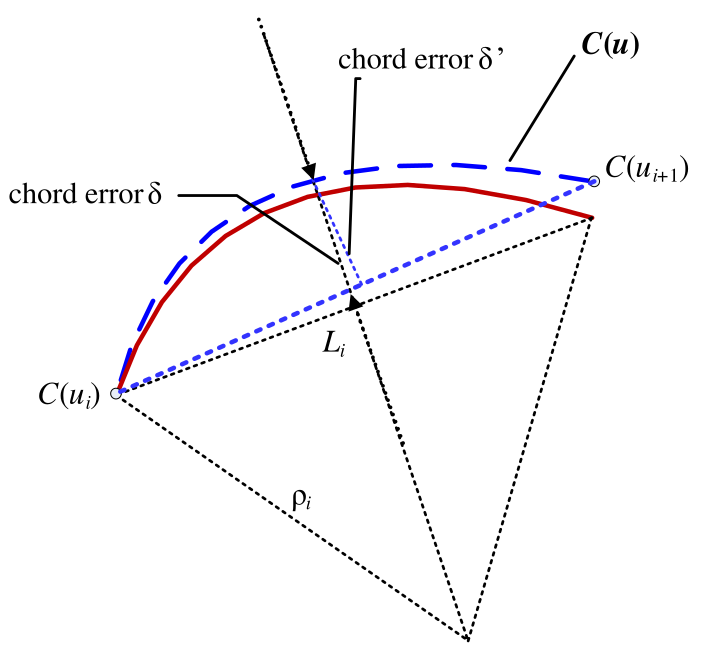
\includegraphics[width=0.60\textwidth]{Images/Chap3/Chord-error-between-2-interpolated-points.png} 
	\caption{Chord-error between two interpolated points}
	\label{Chord-error-between-2-interpolated-points.png}
\end{figure}

\clearpage
\pagebreak


\section{Feedrate or Velocity $ \textbf{V(u)} $}

This section describes the derivation of feedrate or velocity ($V(u_{i})$) from the radius of curvature ($rho(u_{i})$) and chord-error ($eps(u_{i})$). For a linear distance traveled (chord distance) between $C(u_{i})$ and $C(u_{i+1})$, denoted by $L_{i}$, the velocity is given by

\[ V(u_{i}) = \frac {L_{i}} {T_{i}}  \] 

where $T_{i} = (t_{i+1} - t_{i})$  is the interpolation time. Since an arc approximates a section of the circle, the chord error $eps(u_{i})$, is derived from geometry as a function of the radius of curvature $rho(u_{i})$, approximately as follows:

\[ eps(u_{i}) = (radius\_to\_arc) - (radius\_to\_center\_of\_chord) \]

\[ eps(u_{i}) = rho(u_{i}) - \sqrt{{rho(u_{i})}^{2} - {(L_{i}/2)}^{2}}  \]

\vspace{0.5cm}
Solving for $L_{i}$ and replacing for $L_{i}$, the velocity is 

\[ V(u_{i}) = \frac {L_{i}} {T_{i}}   = \frac{2}{T_{i}}.\sqrt{{rho(u_{i})}^{2} - {(rho(u_{i}) - eps(u_{i}))}^{2} } \]   

% \vspace{0.5cm}


% ======================================
\clearpage
\pagebreak

\section{First order Taylor's approximation u\_next(u)}

Consider the parametric curve function C(u), and the time function u(t) as the curve parameter moves from $u(t_{i}) = u_{i}$ to $u(t_{i+1}) = u_{i+1}$. By using a Taylor's expansion, the approximation up to the first derivative is

\[ u(t_{i+1}) = u(t_{i}) + (t_{i+1} - t_{i} ).{\Bigg ( \odv{u}{t} \Bigg ) \Bigg |_{t=t_{i}}} + Higher\_order\_terms \]


\[ u_{i+1} = u_{i} + (t_{i+1} - t_{i} ).{\Bigg ( \odv{u}{t} \Bigg ) \Bigg |_{t=t_{i}}} + Higher\_order\_terms \]

The speed $V(u_{i})$ with respect to time at $u_{i}$ from the parametric curve $C(u)$ is 

\[  V(u_{i}) = \Bigg ( \odv{C(u)}{u} \Bigg ) \Bigg |_{u=u_{i}}. \Bigg ( \odv{u}{t} \Bigg ) \Bigg |_{t=t_{i}} \]

Rearranging the equation 

\[ {\Bigg ( \odv{u}{t} \Bigg ) \Bigg |_{t=t_{i}}} = \frac {V(u_{i})} {\Bigg ( \odv{C(u)}{u} \Bigg ) \Bigg |_{u=u_{i}}} \]

The Taylor's expansion now becomes

\[ u_{i+1} = u_{i} + (t_{i+1} - t_{i} ). \frac {V(u_{i})} {\Bigg ( \odv{C(u)}{u} \Bigg ) \Bigg |_{u=u_{i}}} + Higher\_order\_terms \]
\vspace{0.5cm} 

Neglecting the higher order terms and with the interpolation time or step time defined as $T_{i} = (t_{i+1} - t_{i})$  
\[ u_{i+1} = u_{i} +   unext1(u)\]
\[ u_{i+1} = u_{i} +  \frac {(T_{i}).V(u_{i})} {\Bigg ( \odv{C(u)}{u} \Bigg ) \Bigg |_{u=u_{i}} }\]
\vspace{0.5cm} 

Note that the denominator cannot be zero.

% ================================
\clearpage
\pagebreak

\section{Second order Taylor's approximation u\_next(u)}

\noindent Define the interpolation time $T_{i} = (t_{i+1} - t_{i})$    
\vspace{0.5cm}   

%% $
%% \frac{\mathrm{d^2}u(t)}{\mathrm{d}t^2} 
%%
%% \frac{\mathrm{d^2}x(u)}{\mathrm{d}u^2}
%% $ 


By using a Taylor's expansion, the approximation up to the second derivative is

\[ u(t_{i+1}) = u(t_{i}) + (T_{i}).{\Bigg ( \frac{\mathrm{d}u(t)}{\mathrm{d}t}  \Bigg ) \Bigg |_{t=t_{i}}} + \frac{T_{i}^{2}}{2}.{\Bigg ( \frac{\mathrm{d^2}u(t)}{\mathrm{d}t^2} \Bigg ) \Bigg |_{t=t_{i}}} + Higher\_order\_terms \]

Neglecting the higher order terms,

\[ u(t_{i+1}) = u(t_{i}) + (T_{i}).{\Bigg ( \frac{\mathrm{d}u(t)}{\mathrm{d}t} \Bigg ) \Bigg |_{t=t_{i}}} + \frac{T_{i}^{2}}{2}.{\Bigg ( \frac{\mathrm{d^2}u(t)}{\mathrm{d}t^2}  \Bigg ) \Bigg |_{t=t_{i}}} \]

\[\Bigg (  \frac{\mathrm{d^2}u(t)}{\mathrm{d}t^2} \Bigg ) =  \odv{\Bigg (\frac{\mathrm{d}u(t)}{\mathrm{d}t}   \Bigg)}{t} = \odv{f(t)}{t}  \]

\vspace{0.5cm}  

Given arbitrary functions f(t), g(t) and h(t), where: 
\[ f(t) = \frac {g(t)}{h(t)} \]

The Quotient Rule says that the derivative of a quotient is the denominator times the derivative of the numerator minus the numerator times the derivative of the denominator, all divided by the square of the denominator. Using the quotient rule for the derivative gives:

\[ \odv{f(t)}{t} = \frac { h(t). \Bigg( \odv{g(t)}{t} \Bigg) - g(t).\Bigg( \odv{h(t)}{t} \Bigg)} {( h(t) )^{2}  } \]

With the function f(t) calculated previously

\[ f(t) = \Bigg ( \odv{u(t)}{t} \Bigg )  =  \frac {V(u_{i})} {\Bigg ( \odv{C(u)}{u} \Bigg ) \Bigg |_{u=u_{i}}} \]

\[ \odv{f(t)}{t}  = \Bigg ( \frac{\mathrm{d^2}u(t)}{\mathrm{d}t^2}  \Bigg ) = \odv{\Bigg( g(t)/h(t) \Bigg) }{t}  \]
where
\[ g(t) = V(u_{i}) \]
\[ h(t) = \Bigg ( \odv{C(u)}{u} \Bigg ) \Bigg |_{u=u_{i}}\]

Substitute g(t) and h(t) into the quotient rule equation and rearranging

\[ \odv{f(t)}{t} = \Bigg ( \frac{\mathrm{d^2}u(t)}{\mathrm{d}t^2} \Bigg )  = - {(V(u_{i}))}^{2}. \frac{A}{B} \]

\[ \Bigg ( \frac{\mathrm{d^2}u(t)}{\mathrm{d}t^2} \Bigg )  = - {(V(u_{i}))}^{2}. \frac{ \Bigg | {\Bigg (\frac{\mathrm{d^2}C(u)}{\mathrm{d}u^2} \Bigg ) \Bigg |_{u=u_{i}} } }{ \Bigg | {\Bigg ( \odv{C(u)}{u} \Bigg ) \Bigg |_{u=u_{i}} ^{3} }    }  \]

where 

\[ A = \Bigg | {\Bigg ( \frac{\mathrm{d^2}C(u)}{\mathrm{d}u^2} \Bigg ) \Bigg |_{u=u_{i}} }  \]
\[ B = \Bigg | {\Bigg ( \odv{C(u)}{u} \Bigg ) \Bigg |_{u=u_{i}} ^{3} }  \]

The second order Taylor's expansion for the function u(t) becomes
\[ u(t_{i+1}) = u(t_{i}) + (T_{i}).{\Bigg ( \odv{u}{t} \Bigg ) \Bigg |_{t=t_{i}}} + \frac{T_{i}^{2}}{2}.{\Bigg ( \frac{\mathrm{d^2}u}{\mathrm{d}t^2} \Bigg ) \Bigg |_{t=t_{i}}} \]

\[ u(t_{i+1}) = u(t_{i}) + \frac{(T_{i}.V(u_{i}))} {\Bigg ( \odv{C(u)}{u} \Bigg ) \Bigg |_{u=u_{i}}} - \frac{ (T_{i}.V(u_{i})) ^{2}}{2}. \frac{ \Bigg | {\Bigg ( \frac{\mathrm{d^2}C(u)}{\mathrm{d}u^2} \Bigg ) \Bigg |_{u=u_{i}} } }{ \Bigg | {\Bigg ( \odv{C(u)}{u} \Bigg ) \Bigg |_{u=u_{i}} ^{3} } } \]

In software implementation,
\[ u\_next = u(t_{i+1}) - u(t_{i}) \]
\[ u\_next =  \frac{(T_{i}.V(u_{i}))} {\Bigg ( \odv{C(u)}{u} \Bigg ) \Bigg |_{u=u_{i}}} - \frac{ (T_{i}.V(u_{i})) ^{2}}{2}. \frac{ \Bigg | {\Bigg (  \frac{\mathrm{d^2}C(u)}{\mathrm{d}u^2} \Bigg ) \Bigg |_{u=u_{i}} } }{ \Bigg | {\Bigg ( \odv{C(u)}{u} \Bigg ) \Bigg |_{u=u_{i}} ^{3} } } \]
where
\[ \Bigg | \Bigg ( \odv{C(u)}{u} \Bigg ) \Bigg |_{u=u_{i}}  = fxn\_cvel\_magn(u) \]
\[ \Bigg | \Bigg ( \frac{\mathrm{d^2}C(u)}{\mathrm{d}u^2} \Bigg ) \Bigg |_{u=u_{i}} = fxn\_cacc\_magn(u) \]

\[  T_{i}    = (t_{i+1} -t_{i}) = implementation\_time\_selected     \]
\[  V(u_{i}) = velocity\_command\_or\_feedrate\_generated\_by\_some\_function \]

% =======================================
%% \clearpage
%% \pagebreak

\section{Next interpolation point calculation}

In the realtime interpolation algorithm, the next interpolation point $u\_next$ is calculated based on Taylor's expansion as follows. Note that for $u\_next$ to be valid, the denominators cannot be zero.\\

\textbf{First order Taylor's approximation}
\[ u\_next = \frac {(T_{i}).V(u_{i})} {\Bigg ( \odv{C(u)}{u} \Bigg ) \Bigg |_{u=u_{i}} } \]
\vspace{0.5cm}

\textbf{Second order Taylor's approximation}
\[ u\_next =  \frac{(T_{i}.V(u_{i}))} {\Bigg ( \odv{C(u)}{u} \Bigg ) \Bigg |_{u=u_{i}}} - \frac{ (T_{i}.V(u_{i})) ^{2}}{2}. \frac{ \Bigg | {\Bigg ( \frac{\mathrm{d^2}C(u)}{\mathrm{d}u^2} \Bigg ) \Bigg |_{u=u_{i}} } }{ \Bigg | {\Bigg ( \odv{C(u)}{u} \Bigg ) \Bigg |_{u=u_{i}} ^{3} } } \]
\vspace{0.5cm}

The above are the two(2) equations to be used in software implementation. Notice the negative value of the second term in the Second order Taylor's approximation. \\

It is important to note that all of the derivatives (first and second order) are executed on the curve C(u) with respect to  parameter u. The time parameter t is no longer in the equation. Essentially, the Taylor's approximation used here "transforms" the u\_next point in terms of u instead of t. The starting point is u being a "function of t, that is, u(t)".\\



% ======================================================

% ======================================================
\clearpage
\pagebreak

\section{Feedrate limit calculations}

The current feedrate limit is the minimum of four(4) separate feedrate limits denoted by $ \Big (fratelimit\_1, fratelimit\_2, fratelimit\_3, fratelimit\_4 \Big)$. The limits are based on geometrical and dynamical constraints described below. \\

\begin{table}[!ht]
\begin{center}
%% \caption{Feedrate limit parameters}	
%% \label{Feedrate-limit-parameters}	
\begin{tabular}{ p{2.0cm} p{13.0cm} }
%% \hline
    $fratelimit\_1$ & = frate\_command, a user specified feedrate constraint value\\   
& \\
	$fratelimit\_2$ & = dynamic constraint on machine maximum X-Y axial velocities \\   
& \\
	$fratelimit\_3$ & = geometric constraint on chord-error or contour accuracy \\   
& \\
	$fratelimit\_4$ & = dynamic constraint on machine maximum X-Y axial accelerations \\   
& \\
%% \hline
\end{tabular}
\end{center}
\end{table}

\noindent The functional form for the current feedrate limit becomes: \\

\noindent feedrate\_limit = $\textbf{min}\Big (fratelimit\_1, fratelimit\_2, fratelimit\_3, fratelimit\_4 \Big)$ \\

\noindent The current feedrate limit at $u$ is caclulated as a function of the following variables.\\

\begin{table}[!ht]
	\begin{center}
		\caption{Feedrate limit function parameters}	
		\label{Feedrate-limit-parameters}	
		\begin{tabular}{ p{3.0cm} p{11.0cm} }
			\hline 
			$rt$               & = current runtime in seconds \\
			$u$                & = current $u$ parameter value \\
			$u\_next$          & = next interpolated $u$ parameter value \\
			$FC$               & = user specified feedrate command (constant) value  \\
			$T$                & = interpolation step time (constant 0.001) in seconds\\
			$rho$              & = radius of curvature at current $u$ value  \\ 
			$eps$              & = chord-error (epsilon) at current $u$ value \\
			$lambda$           & = safety factor for acceleration (a constant, range 0.0 - 1.0) \\ 
			$xVel_{max}$ & = maximum allowable x-axis velocity of the machine \\
			$yVel_{max}$ & = maximum allowable y-axis velocity of the machine \\
			$xAcc_{max}$ & = maximum allowable x-axis acceleration of the machine \\
			$yAcc_{max}$ & = maximum allowable y-axis acceleration of the machine \\
			$alphaVel$   & = magnitude of x-velocity unit vector at current $u$\\
			$betaVel$    & = magnitude of y-velocity unit vector at current $u$\\
			\hline
		\end{tabular}
	\end{center}
\end{table}

It is important to note that the feedrate limit calculations for the Teardrop curve were conducted as a comparison to the work of \cite{Zhong-etal:2018}. The calculations overall were different, but the resulting feedrate profiles were similar. This work however, produces a much smoother feedrate profile. 


%% ==================================================
\clearpage
\pagebreak

\subsection{Feedrate Limit 1}

\begin{table}[ht]
\begin{center}
\begin{tabular}{ p{14.0cm} }
\caption{Calculation for fratelimit\_1}
\begin{eqnarray}
	fratelimit\_1 & = & user\_assigned\_fixed\_value (e.g. 20) \nonumber
\end{eqnarray}
\end{tabular}
\end{center}
\end{table}

The machining feedrate during correct machine operation should never exceed this user assigned feedrate value. Thus, $fratelimit\_1$ is the absolute maximum limit, and therefore, appropriately termed as the $feedrate\_command$. For a perfect and ideal operation, the machine should be running at this feedrate value throughout the curve path. This should happen for a path that is exactly a straight line.

\subsection{Feedrate Limit 2}

\begin{table}[ht]
\begin{center}
\begin{tabular}{ p{14.0cm} }
\caption{Calculation for fratelimit\_2}
\begin{eqnarray}
	alphaVel(u) & = &  \Bigg | \frac { \Bigg (\odv{x(u)}{u} \Bigg) } { \sqrt { \Bigg( {\odv{x(u)}{u}} \Bigg )^{2} +  \Bigg ( {\odv{y(u)}{u}} \Bigg )^{2} } }  \Bigg |  \nonumber \\
	betaVel(u)  & = &  \Bigg | \frac { \Bigg (\odv{y(u)}{u} \Bigg) } { \sqrt { \Bigg( {\odv{x(u)}{u}} \Bigg )^{2} +  \Bigg ( {\odv{y(u)}{u}} \Bigg )^{2} } }  \Bigg |  \nonumber \\
    A & = & xVel_{max} / alphaVel(u) \nonumber \\
    B & = & yVel_{max} / betaVel(u)  \nonumber \\   
    fratelimit\_2 & = & minimum (A, B) \nonumber 
\end{eqnarray}
\end{tabular}
\end{center}
\end{table}

The $fratelimit\_2$ is dependent on both geometrical constraints $alphaVel(u)$ and $betaVel(u)$, as well as dynamical constraints, that is, the maximum allowable axial velocities of the machine as shown above ($xVel_{max}$ and $yVel_{max}$) The quantities $alphaVel(u)$, $betaVel(u)$ are essentially the magnitudes of curve unit vectors in the x and y directions, respectively. 

\subsection{Feedrate Limit 3}

\begin{table}[ht]
\begin{center}
\begin{tabular}{ p{14.0cm} }
\caption{Calculation for fratelimit\_3}
\begin{eqnarray}
numerator(u) & = & \Bigg ( \Bigg ({\odv{x(u)}{u}} \Bigg )^{2} + \Bigg ({\odv{y(u)}{u}}\Bigg )^{2} \Bigg ) ^{3/2}  \nonumber \\
denominator(u) & = & \Bigg(\odv{x(u)}{u}\Bigg)\Bigg(\frac{\mathrm{d^2}y(u)}{\mathrm{d}u^2}\Bigg) - \Bigg(\frac{\mathrm{d^2}x(u)}{\mathrm{d}u^2}\Bigg)\Bigg(\odv{y(u)}{u}\Bigg)  \nonumber \\
rho & = & numerator(u)/denominator(u) \nonumber \\
eps & = & rho - \sqrt{{rho}^{2} - {(L/2)}^{2}} \nonumber \\
fratelimit\_3 & = & (2/T)* \Bigg | \sqrt{( 2*rho*eps - eps^{2})} \Bigg | \nonumber 
\end{eqnarray}
\end{tabular}
\end{center}
\end{table}

The $fratelimit\_3$ is primarily dependent on curve geometry, as seen above involving radius of curvature $rho(u)$ and chord-error $eps(u)$. Both are dependent on the independent parameter $u$ and the curve equations. For example, a perfect circle would give a constant radius of curvature $rho(u)$ and the chord lengths would all be the same.\\

% ======================================================
\clearpage
\pagebreak

\subsection{Feedrate Limit 4}

\begin{table}[ht]
\begin{center}
\begin{tabular}{ p{16.0cm} }
\caption{Calculation for fratelimit\_4}
\begin{eqnarray}
	lamda  & = & user\_select\_safety\_factor(0.0 to 1.0)     \nonumber \\
	C & = & \sqrt {\frac{lamda*rho*xAcc_{max}} { \Bigg |(betaVel) \Bigg |} } \nonumber \\
	D & = & \sqrt {\frac{lamda*rho*yAcc_{max}} { \Bigg |(alphaVel)\Bigg |} } \nonumber \\
    fratelimit\_4 & = & minimum (C, D) \nonumber
\end{eqnarray}
\end{tabular}
\end{center}
\end{table}

The $fratelimit\_4$ is dependent on both dynamical and geometrical constraints. The dynamical constraints are in the maximum allowable axial accelerations of the machine as covered by $xAcc_{max}$ and $yAcc_{max}$. The geometrical constraints are in $alphaVel(u)$, $betaVel(u)$ and $rho(u)$.  \\

% ======================================================
\clearpage
\pagebreak


\section{Feedrate rising S-curve}

In CNC machining operation, the feedrate does not rise abruptly from zero. A smooth feedrate rise is required to ensure machine stability. 
A sigmoid S-shaped curve was selected for the rise of the current running feedrate to the current feedrate limit. \\

\[ curr\_frate(rsu) = \frac{curr\_frate\_limit(rsu)} { \Bigg( 1 + e^{(-rsu*rshape1)} \Bigg) ^{rshape2} }  \] \\

\noindent
where the applicable variable range is \\
$rsu\_start\_rise$ $\le$ $rsu$ $\le$ $rsu\_end\_rise$\\

\noindent
The linear parameter transformation from $u$ to $rsu$ is as follows:\\
$rsu$ = $rm*u$ + $rkonst$ \\

To ensure smoothness of the rising feedrate curves, simulations were conducted to determine the best values of the parameters below. These variables are user specified.\\

\begin{table}[!ht]
	\begin{center}
	\caption{Rising S-curve parameters}	
	\label{Rising-S-curve-parameters}	
	\begin{tabular}{ p{3.0cm} p{2.0cm} p{8.0cm}}
    \hline 
	rsu\_start\_rise & = 0.00  & beginning of rising S-curve \nonumber \\
	rsu\_end\_rise   & = 0.05  & end of rising S-curve \nonumber \\
	rshape1          & = 5.00  & S-curve smoothness shaping factor \nonumber \\
	rshape2          & = 8.00  & S-curve smoothness shaping factor \nonumber \\
	rsu1             & = 0.00  & start of u linear transformation\nonumber \\
	rsu2             & = 3.00  & end of u linear transformation \nonumber \\
	rm               & = calc  & slope calculated for each parametric curve \nonumber \\
	rkonst			 & = calc  & constant calculated for each parametric curve \nonumber \\ 
	rsu              & = calc  & transformed variable in the rising S-curve \nonumber \\
    \hline
	\end{tabular}
	\end{center}
\end{table}


% ===============================================
\clearpage
\pagebreak

\section{Flowchart of main interpolation program}

The main program flowchart for the parametric curve interpolation is shown in Fig [\ref{main-10-Main-Program-Algorithm.pdf}]. The parameter update u = u + u\_next is executed for each loop. As shown in the main flowchart, there are 3 main processing modules that cover computations involving u, that is, in the rising, main and falling feedrate sections. \\

The flowchart for the feedrate rising section is shown in  Fig [\ref{01-Feedrate-Rising-Region-flowchart.pdf}], and the feedrate falling section in Fig [\ref{03-Feedrate-Falling-Region-flowchart.pdf}]. The computations for the main section are further separated into 3 cases described below. 

\begin{enumerate}
	
\item When the current\_feedrate is above feedrate\_limit, called CaseA\_(Above), the flowchart is Fig [\ref{02-CaseA1-Feedrate-Above-Limit-Main-Region-flowchart.pdf}] and is continued in Fig [\ref{02-CaseA2-Feedrate-Above-Limit-Main-Region-flowchart.pdf}].

\item When the current\_feedrate is below feedrate\_limit, called CaseB\_(Below), the flowchart is Fig [\ref{02-CaseB1-Feedrate-Below-Limit-Main-Region-flowchart.pdf}] and is continued in Fig [\ref{02-CaseB2-Feedrate-Below-Limit-Main-Region-flowchart.pdf}].
 
\item When the current\_feedrate is equal to the feedrate\_limit, called CaseE (Equal), the flowchart is Fig [\ref{02-CaseE-Feedrate-Equal-Limit-Main-Region-flowchart.pdf}].

\end{enumerate}

The processing in CaseA\_(Above) is basically to push down the running current\_feedrate to just below the calculated feedrate\_limit. On the other hand, the processing in CaseB\_(Below) is to push up the current\_feedrate to also be just below the calculated feedrate\_limit. The net result is the current\_feedrate will be very close but just below the calculated feedrate\_limit.
This is the feedrate constraint part of this work. \\

A common module named Flowchart\_Calculate\_ u\_next(u), is shown in Fig [\ref{04-Calculate-u-next-flowchart.pdf}]. This module will be invoked by the feedrate rising, main and falling modules. This is the implementation of Call-and-Return (CAR) software architecture. \\

%% \clearpage
%% \pagebreak

The Flowchart\_Calculate\_u\_next(u) module will invoke another module named Flowchart\_Calculate\_u\_next(u)\_with\_eps\_pushdown, as shown in Fig [\ref{05-Calculate-u-next-eps-pushdown-flowchart.pdf}]. This last module is responsible for pushing down chord-error (epsilon) below the error tolerance of $(10)^{-6}$. This is the chord-error constraint part of this work.\\
 
Note that a successful effort was also made to push up the value of chord-error to very close but just below the chord-error tolerance, similar to the execution for feedrate constraint. However, this is not a wise move, since increasing the chord error means increasing both total chord-error and total chord length. An increase in chord length means a decrease in total number of interpolated points, a thing that is favorable.\\

However, results showed that there were jitters (severe fluctuations) in feedrate at several segments along the path. The feedrate profile was no longer smooth. Knowing that the chord-error is already below tolerance, the advice taken is to ignore the push up (keep it if it is already below tolerance). And it is sensible because this would keep the total chord-error small and the feedrate profile smooth. Therefore, the chord-error push up idea was abandoned. Only a chord-error push down was executed in the algorithm. 

\clearpage
\pagebreak

It must be the "natural" computation effect in the second order Taylor's expansion for u\_next that generates chord-errors far below error tolerance. Thus, there is no need for intervention to push it up. In addition, this effect ensures smoothness of the feedrate profiles of all curves in this work.\\   
 
This section discusses all the flowcharts in the interpolation algorithm beginning from Fig [\ref{main-10-Main-Program-Algorithm.pdf}] until Fig [\ref{05-Calculate-u-next-eps-pushdown-flowchart.pdf}]. Notice that the algorithm is modular and developed in a structured manner following good software engineering practices. The decision points are well structured and not haphazard, which can cause serious problems like side effects. The problem of side effects will be explained in the section Appendix [App\ref{app-Chap3-About Side Effects in Computations}].  \\

An interesting note in Fig [\ref{main-10-Main-Program-Algorithm.pdf}], the main program flowchart for the entire interpolation, is the existence of "EXIT ON LOGIC ERROR". This exit is an impossible exit, because logically and mathematically it cannot happen. But it was implemented anyway to catch any computational quirks since the algorithm is supposed to cater for ten(10) different parametric curves of various complexities. This quirk can be caused by computations involving numbers below machine-epsilon value. On addition and subtraction, these very small numbers, are treated by computers as "zero", even though the numbers are just very small but truly non-zero. Please refer to Section[\ref{sec-Software engineering practice}] on Software engineering practice that discusses machine-epsilon effects.\\

The impossibility of this "EXIT ON LOGIC ERROR" can be explained as follows. Consider a real number "M", that is compared to another real number "K". \\

\noindent Logically, only three(3) possibilities can happen: \\
(1) M equals K \\
(2) M greater than K \\ 
(3) M less than K \\

\noindent In the case of, "EXIT ON LOGIC ERROR", M is none of the above three(3) possibilities. Thus, it is logically and mathematically impossible. Even though considered impossible, this exit was incorporated to handle quirks and analyze their corresponding causes.

% ======================================================
\clearpage
\pagebreak

%% =============================================
%% MAIN PROGRAM FLOWCHART
%% =============================================

%% PERFECT INCLUDE PDF IN LATEX (AS ONE FULL PAGE)
\begin{figure}
	\caption{Flowchart of main program}
	\label{main-10-Main-Program-Algorithm.pdf}
	\centering
	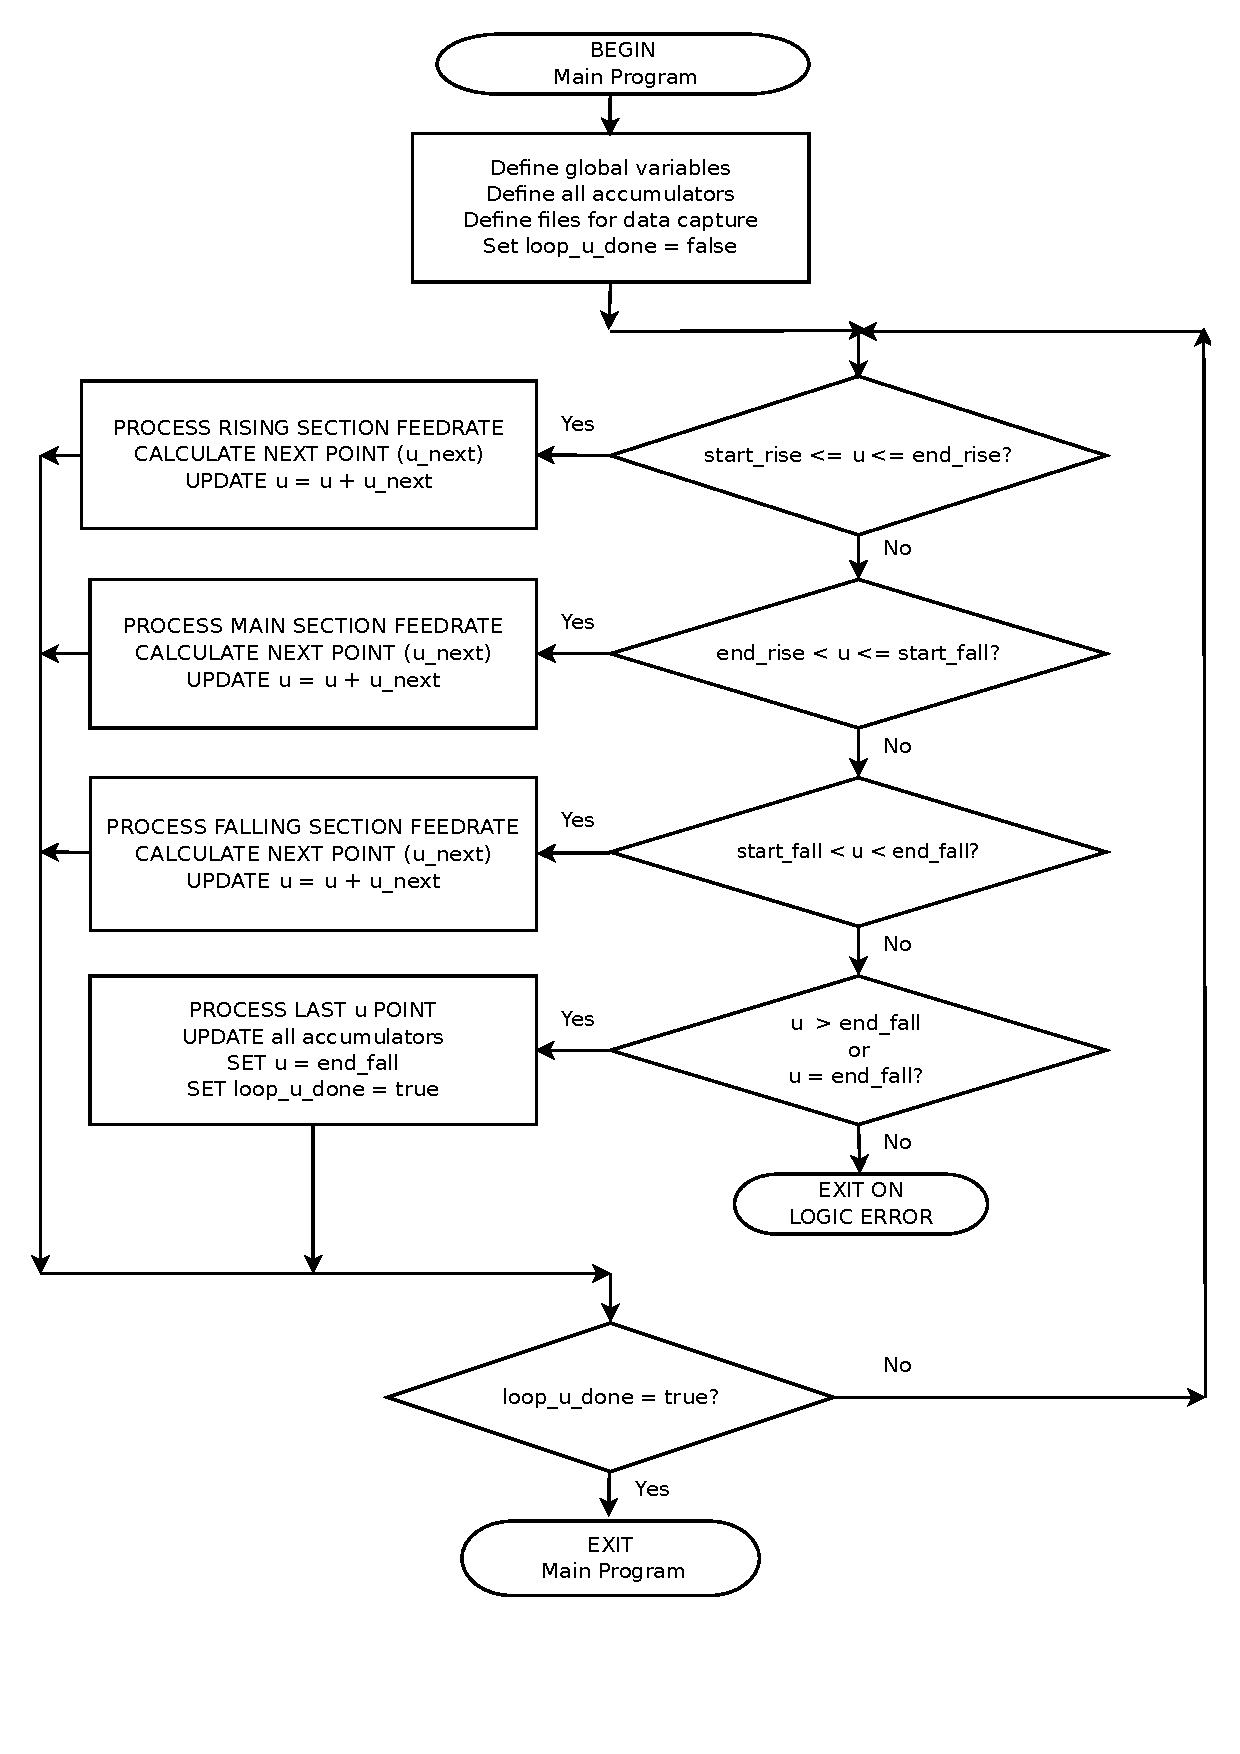
\includegraphics[width=1.15\textwidth,]{Images/Chap3/00-main-10-Main-Program-Algorithm.pdf} 
\end{figure}

%% =============================================
\clearpage
\pagebreak
\section{Feedrate Limit algorithm regions}

\noindent The flow chart for the main program shows that the range of processing is divided into 3 separate regions for $0.0 \le u \le 1.0$ as follows.
\begin{enumerate}
	\item Region ($start\_rise \le u \le end\_rise$), the feedrate rising S-curve region.
	\item Region ($end\_rise < u \le start\_fall$), the feedrate dynamic variation main region.
	\item Region ($start\_fall < u \le end\_fall$), the feedrate falling S-curve region.
\end{enumerate}

\noindent where $start\_rise = 0.0$ and $end\_fall = 1.0$ with ($end\_rise$ and $start\_fall$) user selected.\\ 

\noindent For all parametric curves considered, a large majority of computations for the interpolation algorithm occurs in the feedrate dynamic variation or main region. The feedrate profiles vary markedly from curve to curve.\\

The rising S-curve and falling S-curve sections are regions where the $feedrate\_limit$ are determined by the user assigned rising and falling sigmoid or S-curves. The $feedrate\_limit$ is assigned the exact value according to the rising or falling S-curves. The current or running feedrates are still computed to ensure that the chord-error and running feedrate constraints are observed. In this work, 4 different values of FCs were considered (FC = 10, 20, 30, 40). The execution results are provided in Chapter 4.\\ 

It is important to note that CaseA (Above) and CaseB (Below) are the conditions before processing. During processing, all $current\_feedrates$ are either "iteratively pushed-down" to below and very close to its $feedrate\_limit$, or "iteratively pushed-up" to below and very close to its $feedrate\_limit$. \\

Thus, it effectively means without exception, all $current\_feedrates$ running in operation are below the $feedrate\_limit$ throughout the traversal of the parametric curve. The execution results will be shown in Chapter 4. This condition is called "feedrate constrained", and is one of the main objectives of this thesis.


%% RISING FEEDRATE FLOWCHART
%% =============================================
\clearpage
\pagebreak

%% PERFECT INCLUDE PDF IN LATEX (AS ONE FULL PAGE)
\begin{figure}
	\caption{Flowchart of Feedrate Rising S-Curve}
	\label{01-Feedrate-Rising-Region-flowchart.pdf}
	\centering
	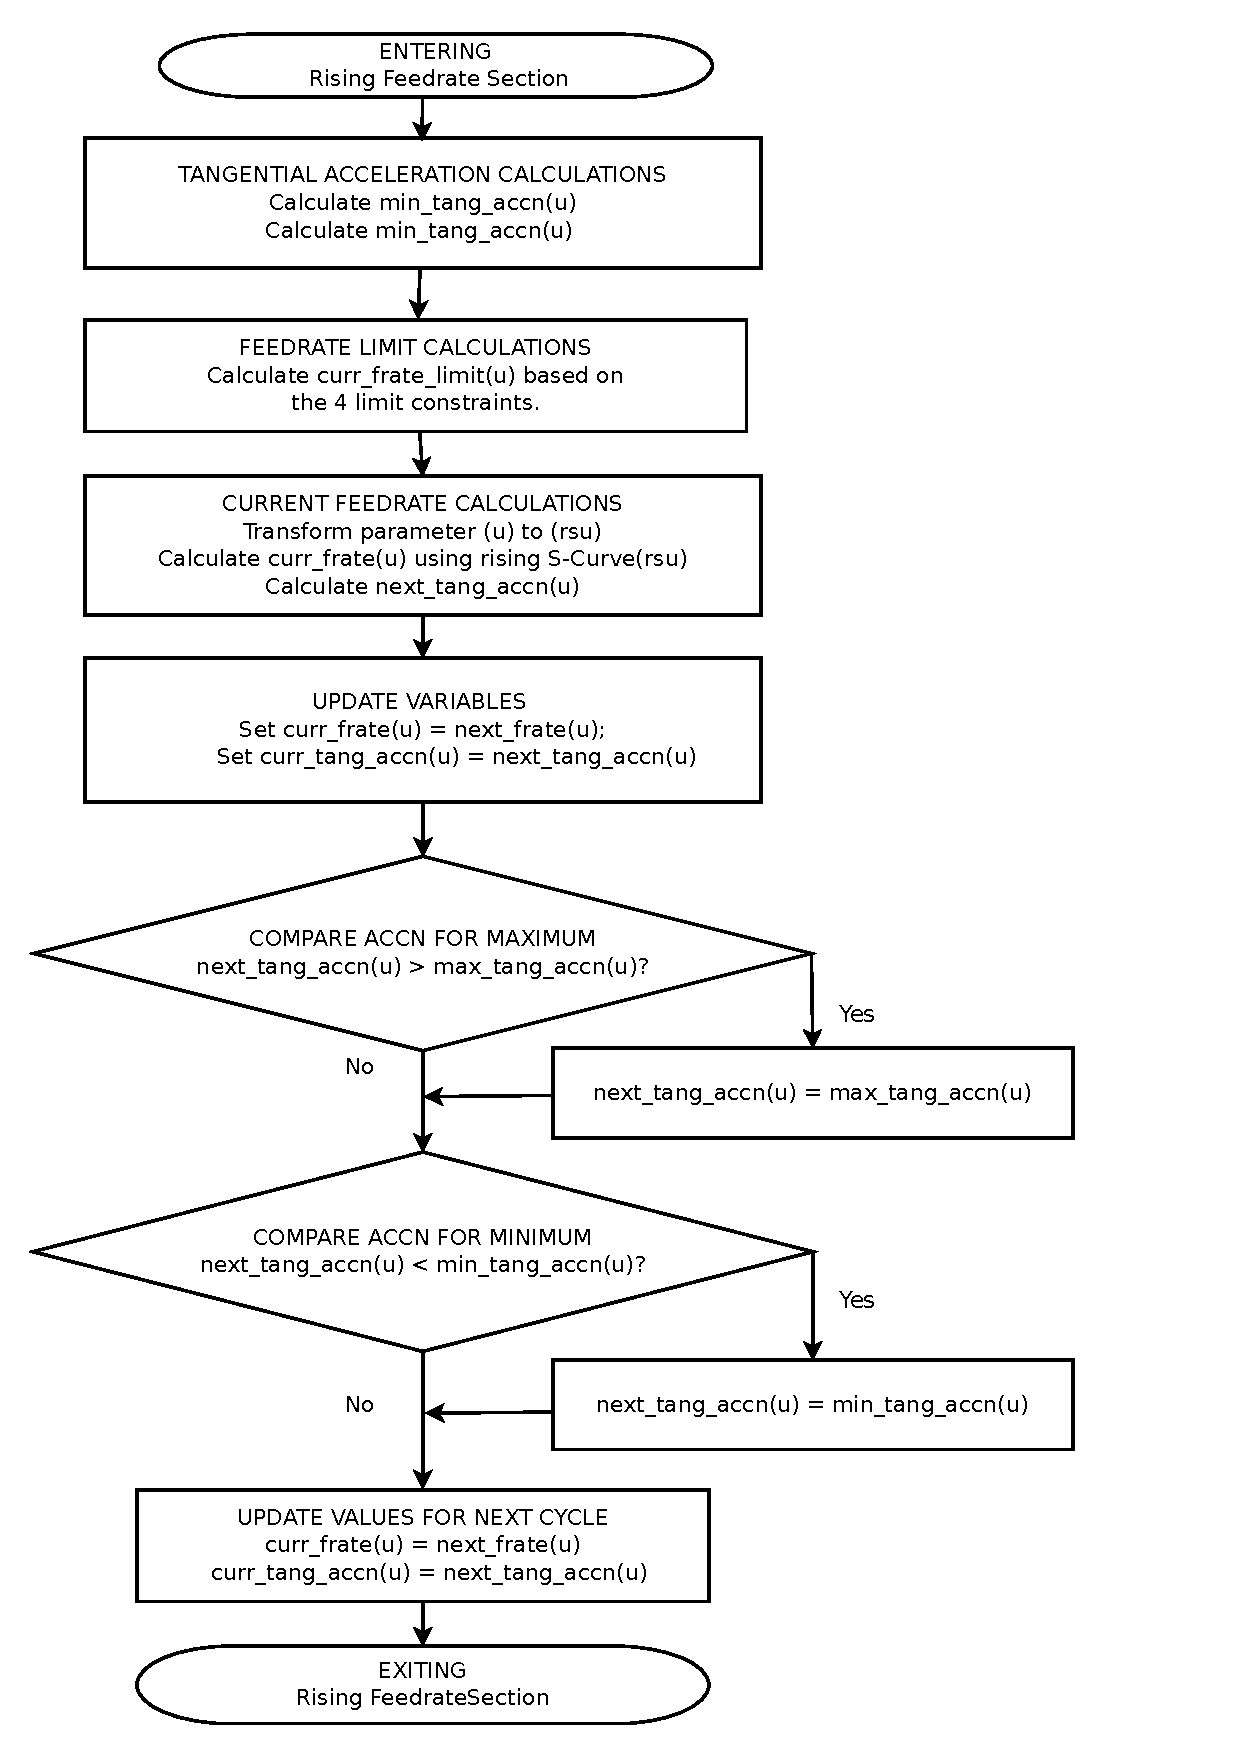
\includegraphics[width=1.10\textwidth,]{Images/Chap3/01-Feedrate-Rising-Region-flowchart.pdf} 
\end{figure}


%% FEEDRATE ABOVE FEEDRATE LIMIT PART 1/2
%% ==============================================
\clearpage
\pagebreak

%% PERFECT INCLUDE PDF IN LATEX (AS ONE FULL PAGE)
\begin{figure}
	\caption{Flowchart Current Feedrate above Feedrate Limit Part 1/2}
	\label{02-CaseA1-Feedrate-Above-Limit-Main-Region-flowchart.pdf}
	\centering
	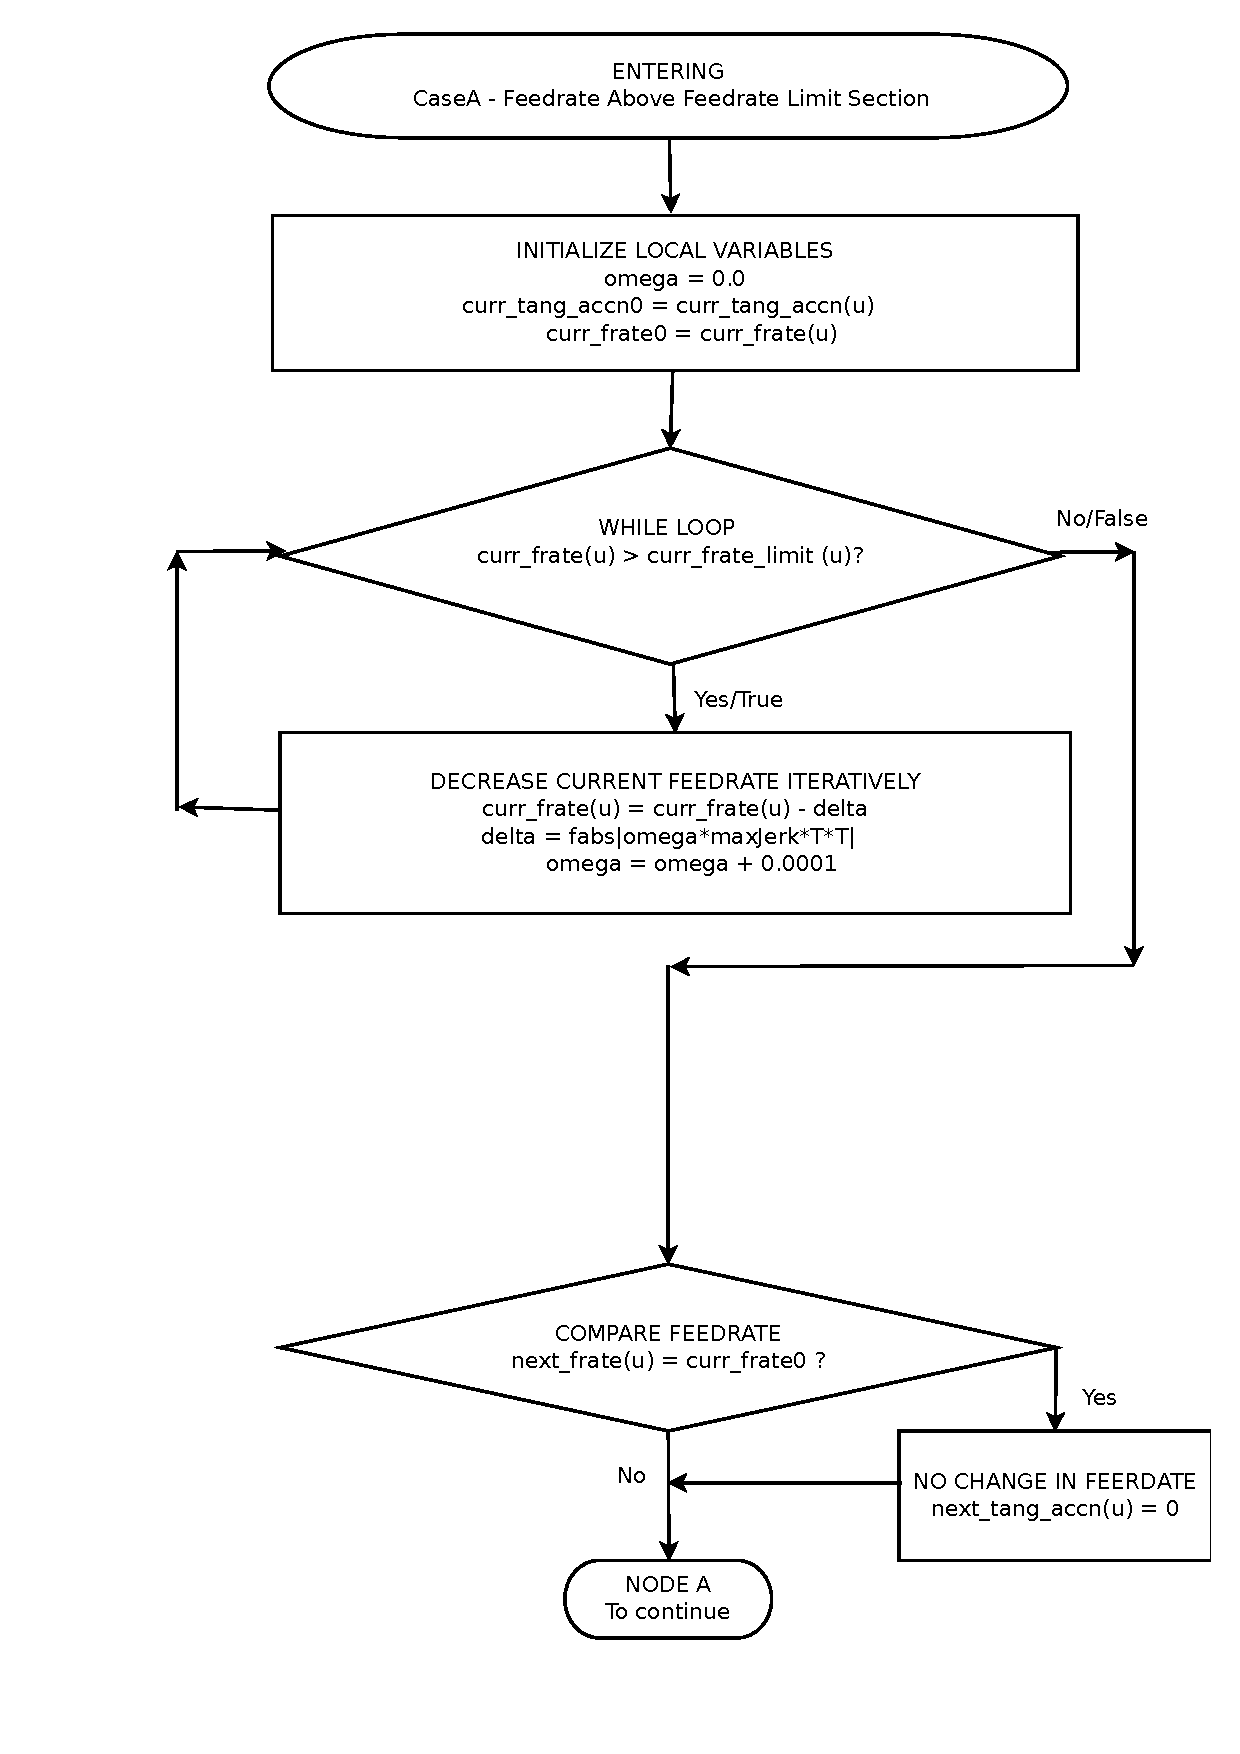
\includegraphics[width=1.10\textwidth,]{Images/Chap3/02-CaseA1-Feedrate-Above-Limit-Main-Region-flowchart.pdf} 
\end{figure}

%% FEEDRATE ABOVE FEEDRATE LIMIT PART 2/2
%% ==============================================
\clearpage
\pagebreak

%% PERFECT INCLUDE PDF IN LATEX (AS ONE FULL PAGE)
\begin{figure}
	\caption{Flowchart Current Feedrate above Feedrate Limit Part 2/2}
	\label{02-CaseA2-Feedrate-Above-Limit-Main-Region-flowchart.pdf}
	\centering
	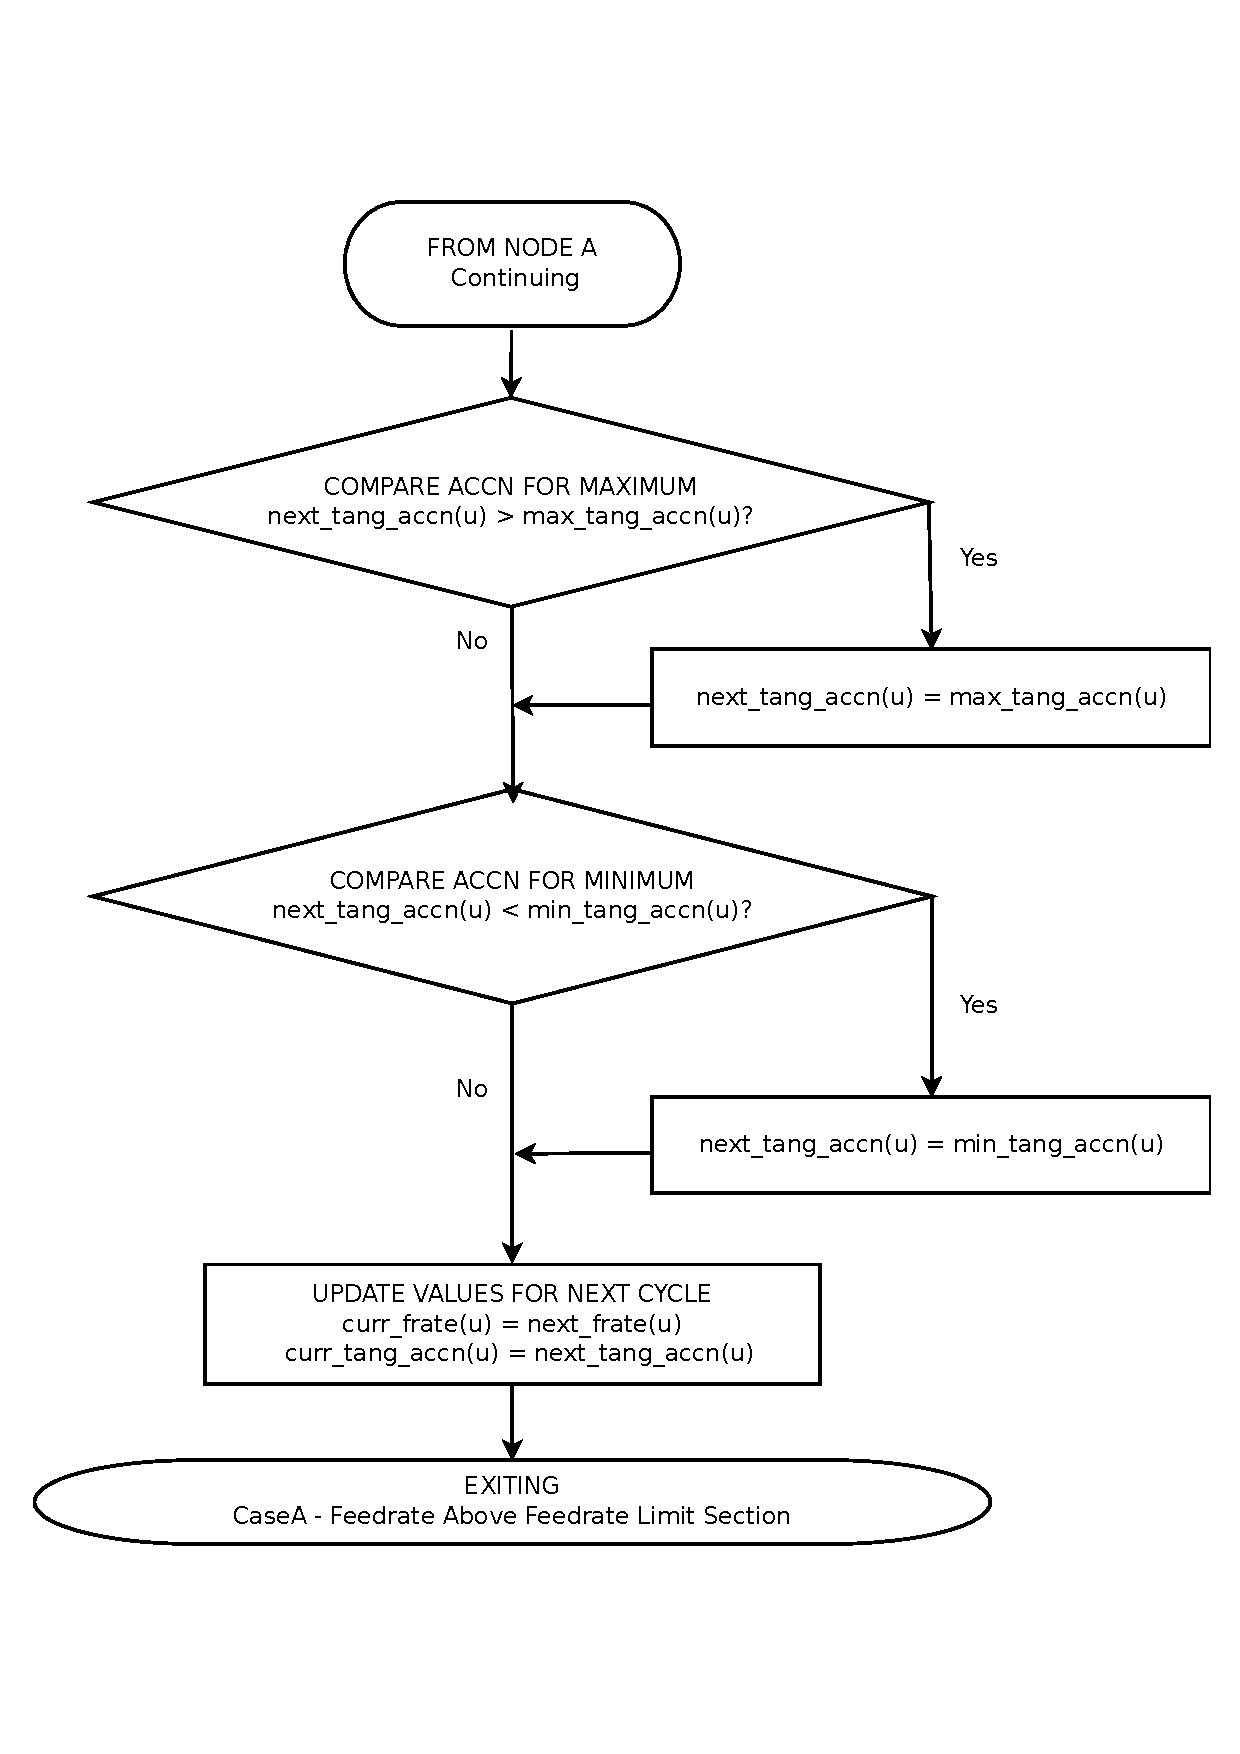
\includegraphics[width=1.10\textwidth,]{Images/Chap3/02-CaseA2-Feedrate-Above-Limit-Main-Region-flowchart.pdf} 
\end{figure}

%% FEEDRATE BELOW FEEDRATE LIMIT PART 1/2
%% =============================================
\clearpage
\pagebreak

%% PERFECT INCLUDE PDF IN LATEX (AS ONE FULL PAGE)
\begin{figure}
	\caption{Flowchart Current Feedrate below Feedrate Limit Part 1/2}
	\label{02-CaseB1-Feedrate-Below-Limit-Main-Region-flowchart.pdf}
	%% \centering
	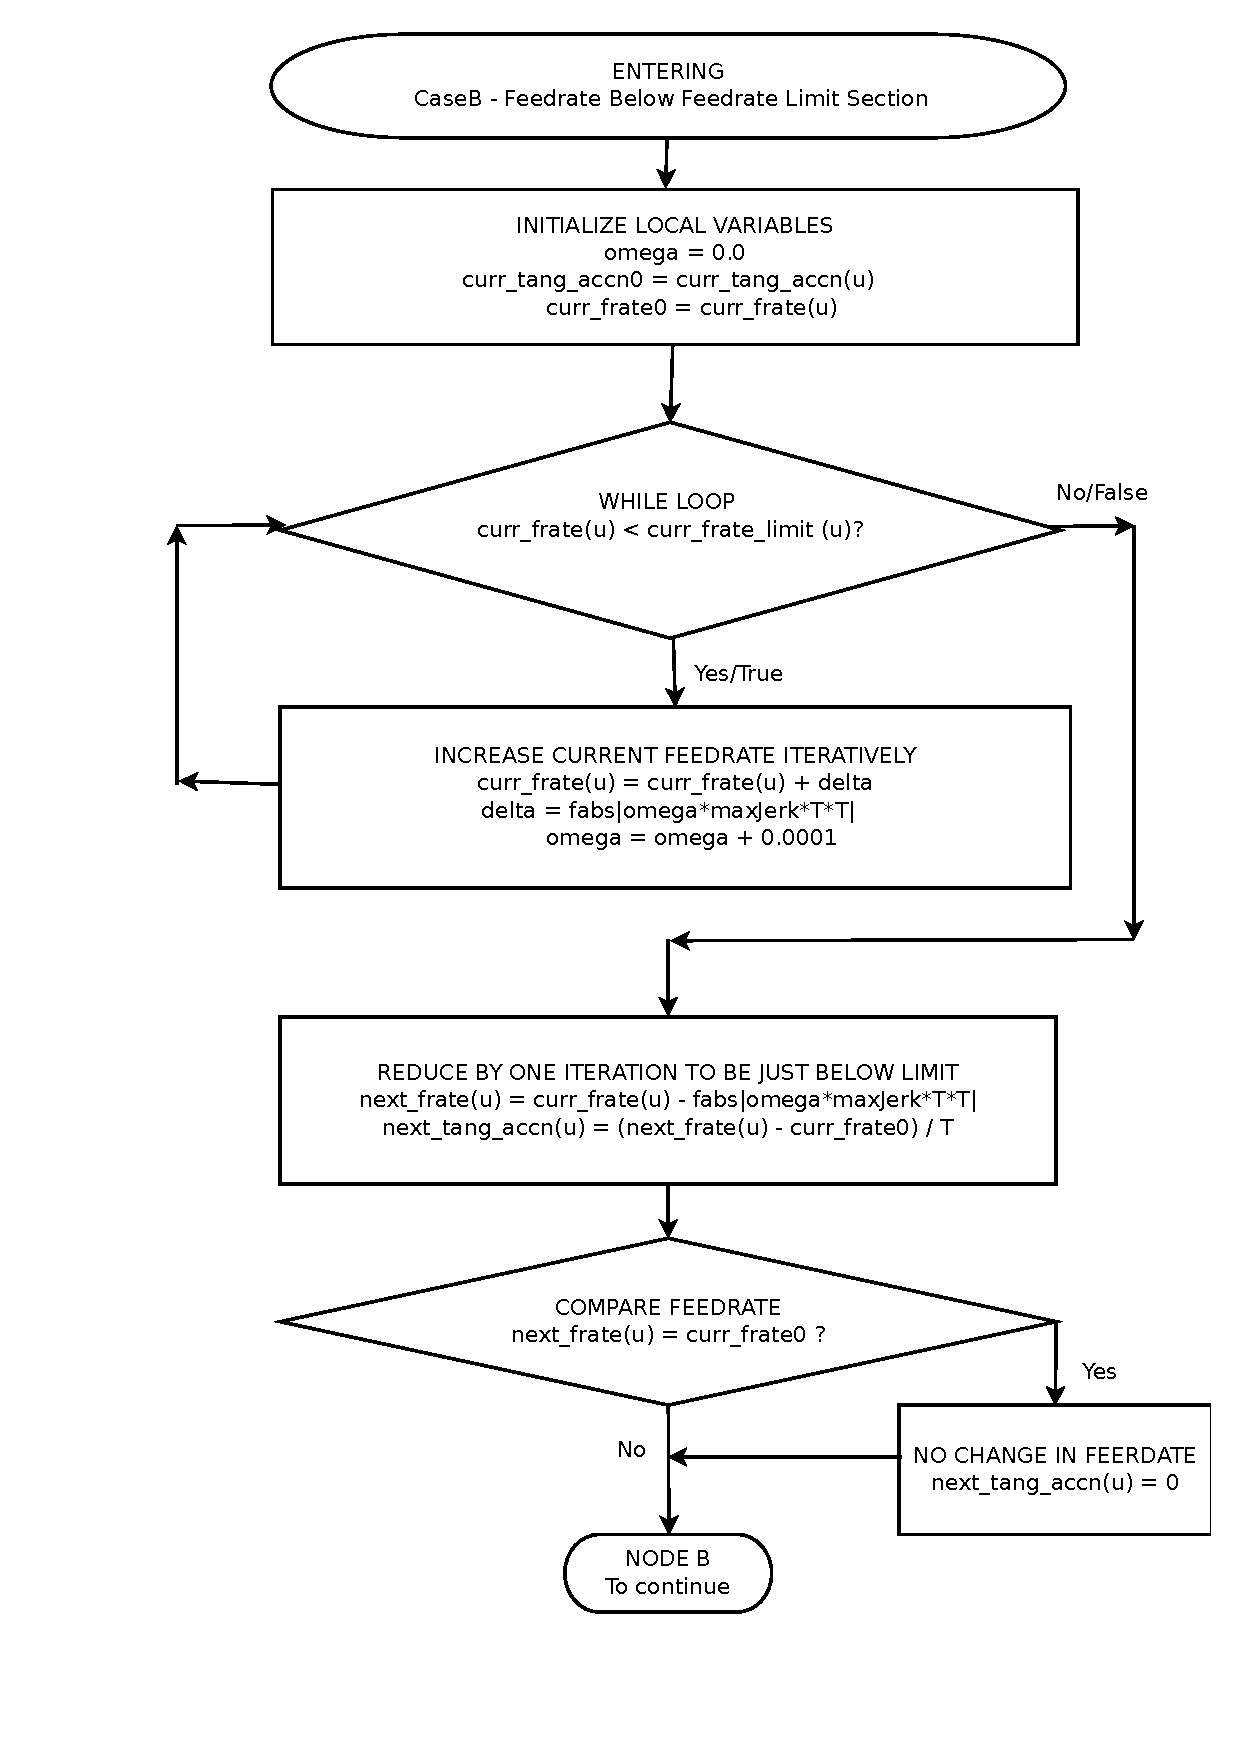
\includegraphics[width=1.10\textwidth,]{Images/Chap3/02-CaseB1-Feedrate-Below-Limit-Main-Region-flowchart.pdf} 
\end{figure}

%% FEEDRATE BELOW FEEDRATE LIMIT PART 2/2
%% =============================================
\clearpage
\pagebreak

%% PERFECT INCLUDE PDF IN LATEX (AS ONE FULL PAGE)
\begin{figure}
	\caption{Flowchart Current Feedrate below Feedrate Limit Part 2/2}
	\label{02-CaseB2-Feedrate-Below-Limit-Main-Region-flowchart.pdf}
	\centering
	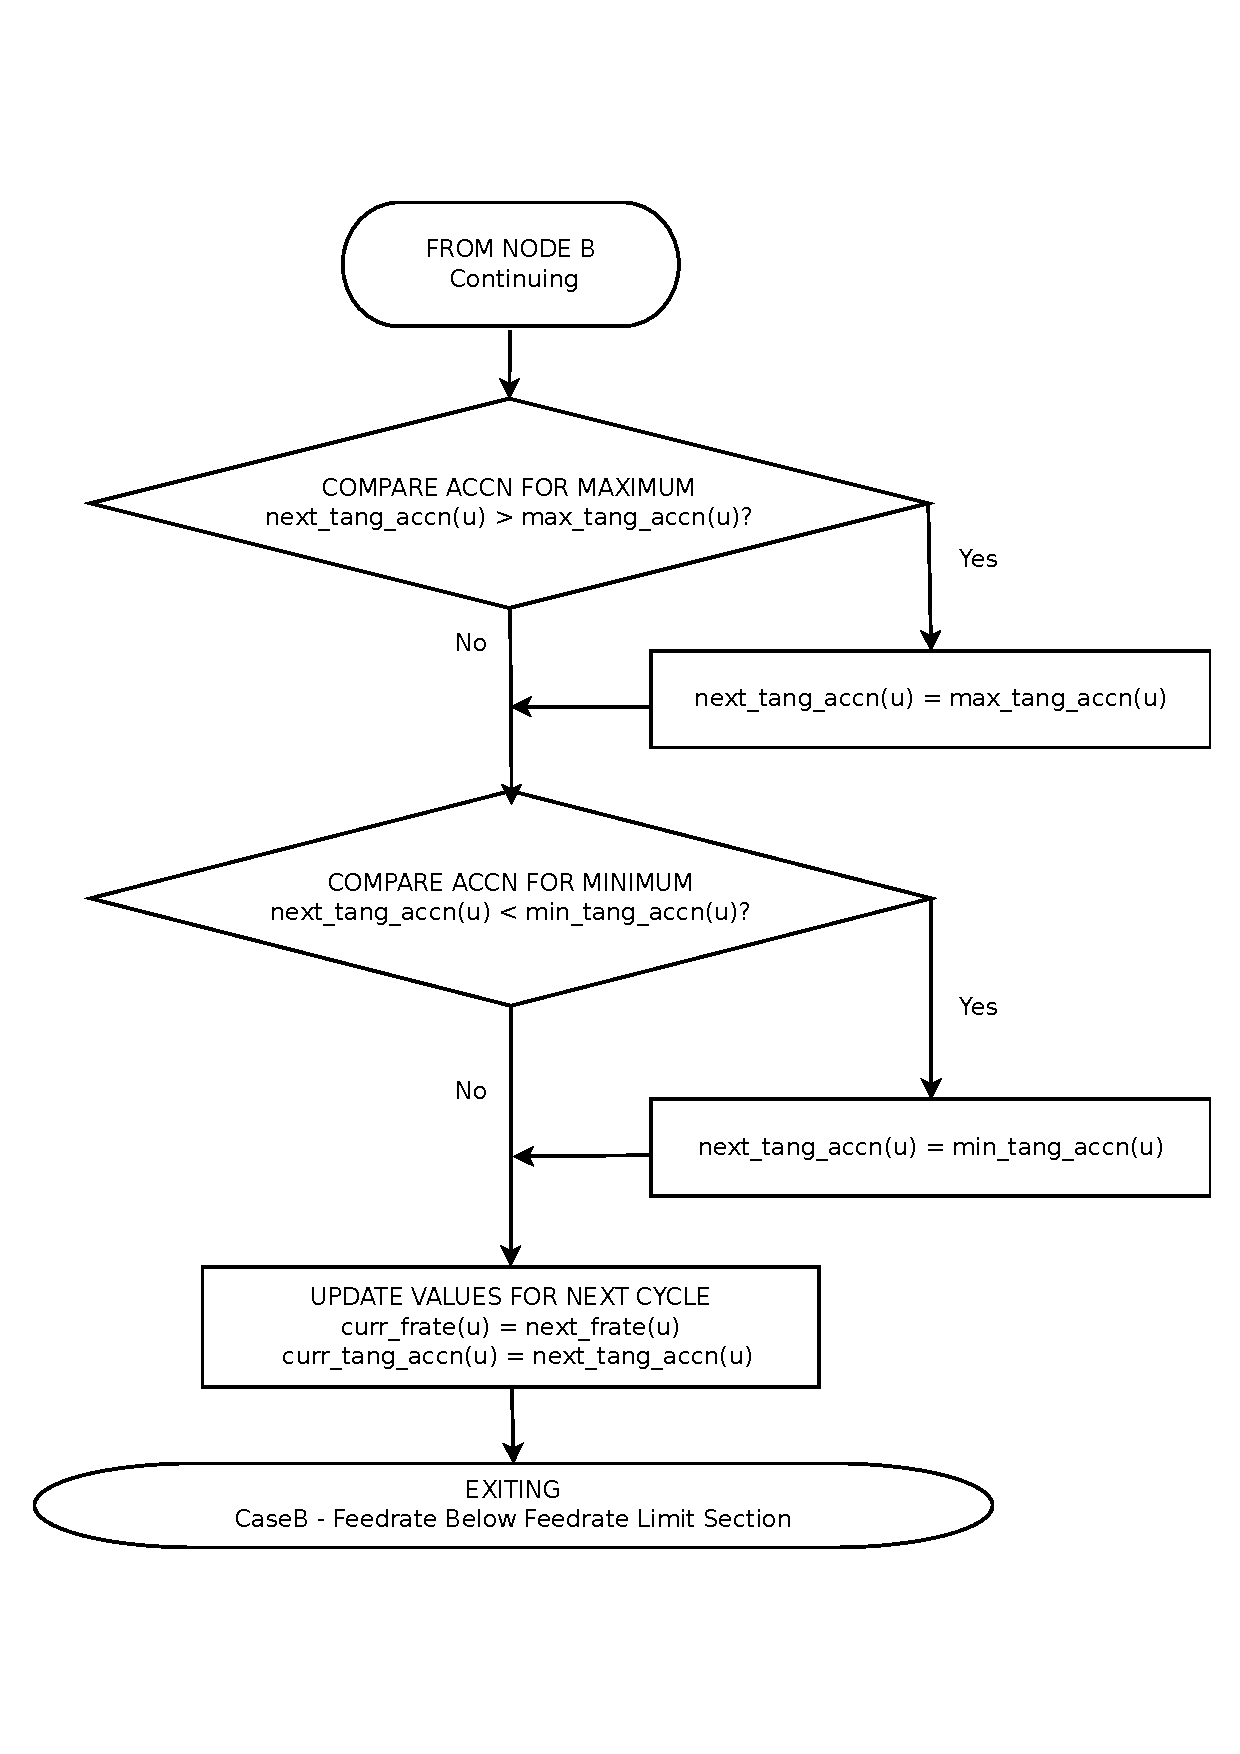
\includegraphics[width=1.10\textwidth,]{Images/Chap3/02-CaseB2-Feedrate-Below-Limit-Main-Region-flowchart.pdf} 
\end{figure}


%% FEEDRATE EQUAL LIMIT 
% =============================================
\clearpage
\pagebreak



%% PERFECT INCLUDE PDF IN LATEX (AS ONE FULL PAGE)
\begin{figure}
	\caption{Flowchart Current Feedrate equal Feedrate Limit}
	\label{02-CaseE-Feedrate-Equal-Limit-Main-Region-flowchart.pdf}
	\centering
	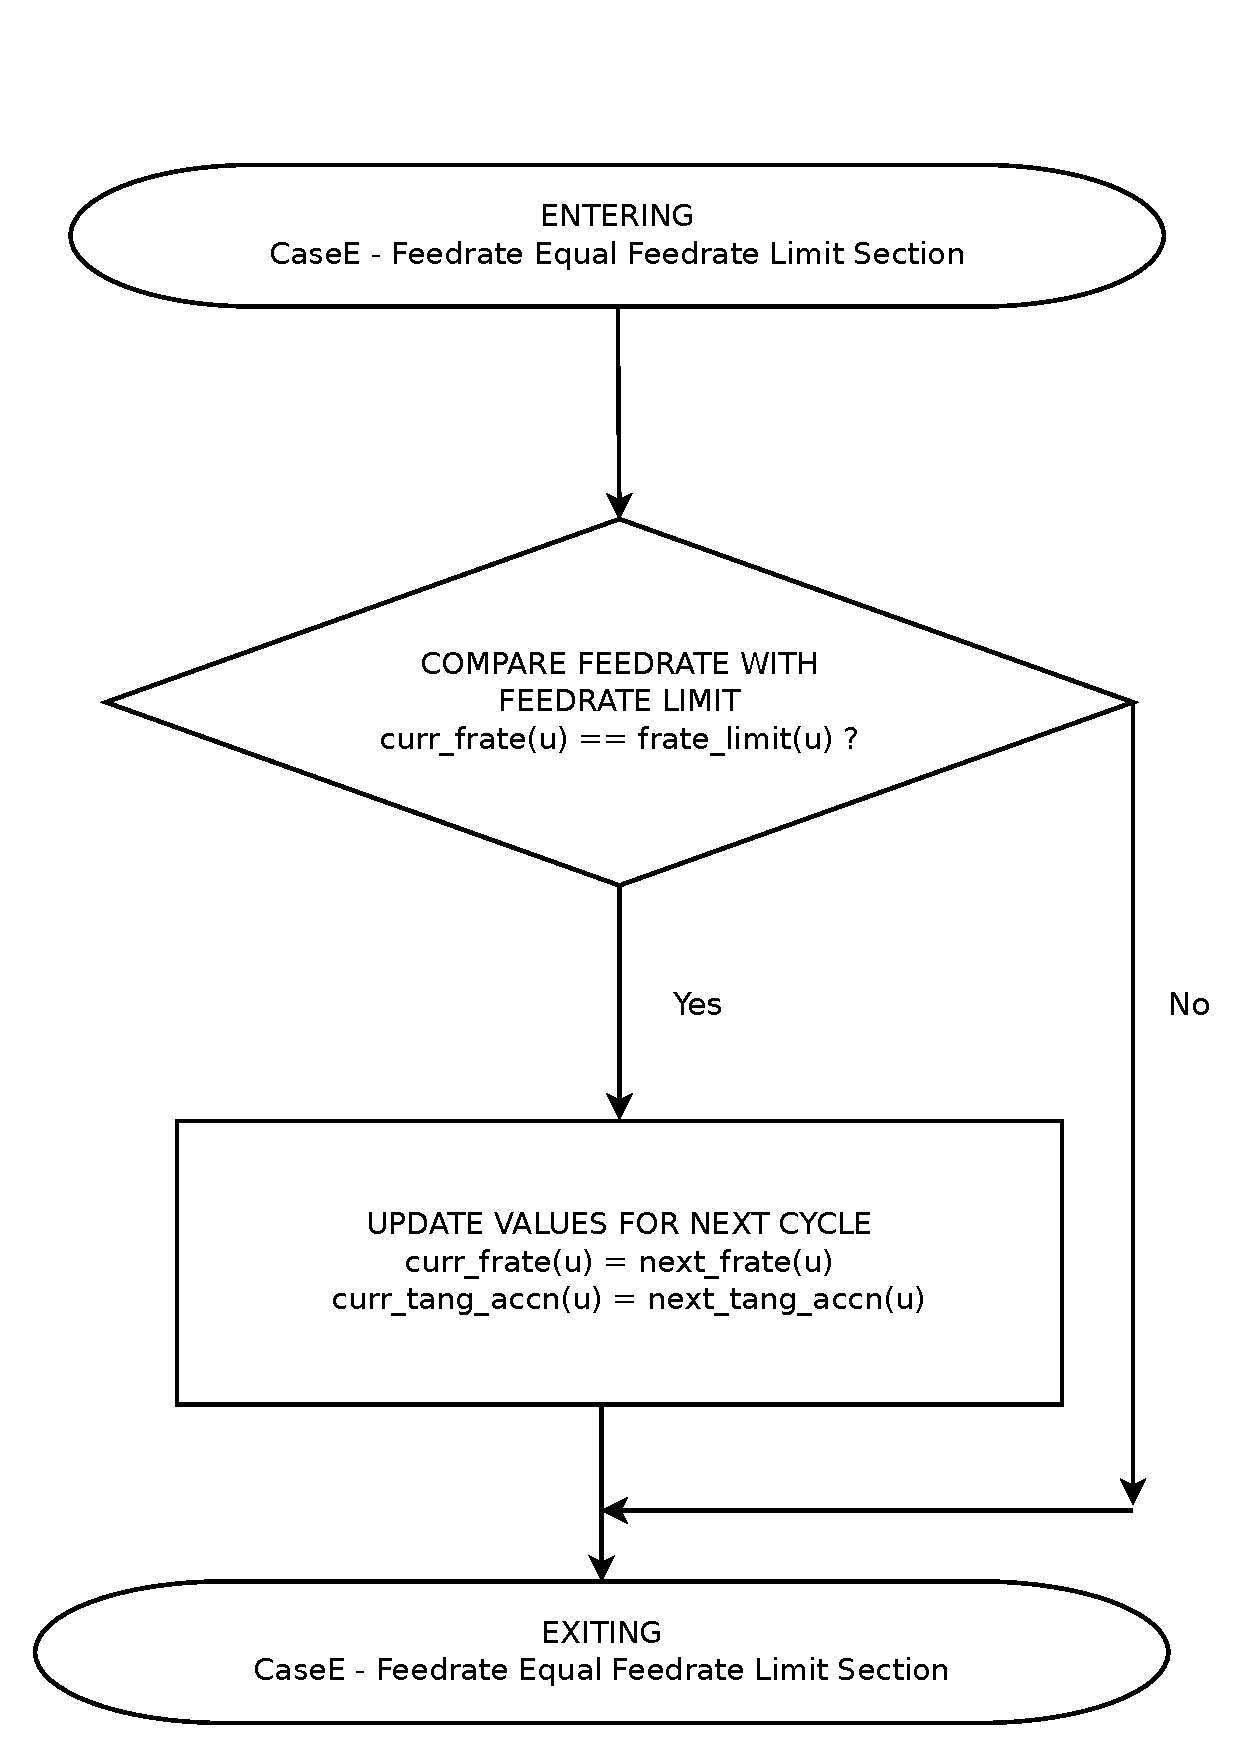
\includegraphics[width=0.85\textwidth,]{Images/Chap3/02-CaseE-Feedrate-Equal-Limit-Main-Region-flowchart.pdf} 
\end{figure}


%% CALCULATE U-NEXT 
%% =============================================
\clearpage
\pagebreak

%% PERFECT INCLUDE PDF IN LATEX (AS ONE FULL PAGE)
\begin{figure}
	\caption{Flowchart Calculate u\_next(u)}
	\label{04-Calculate-u-next-flowchart.pdf}
	%%\centering
	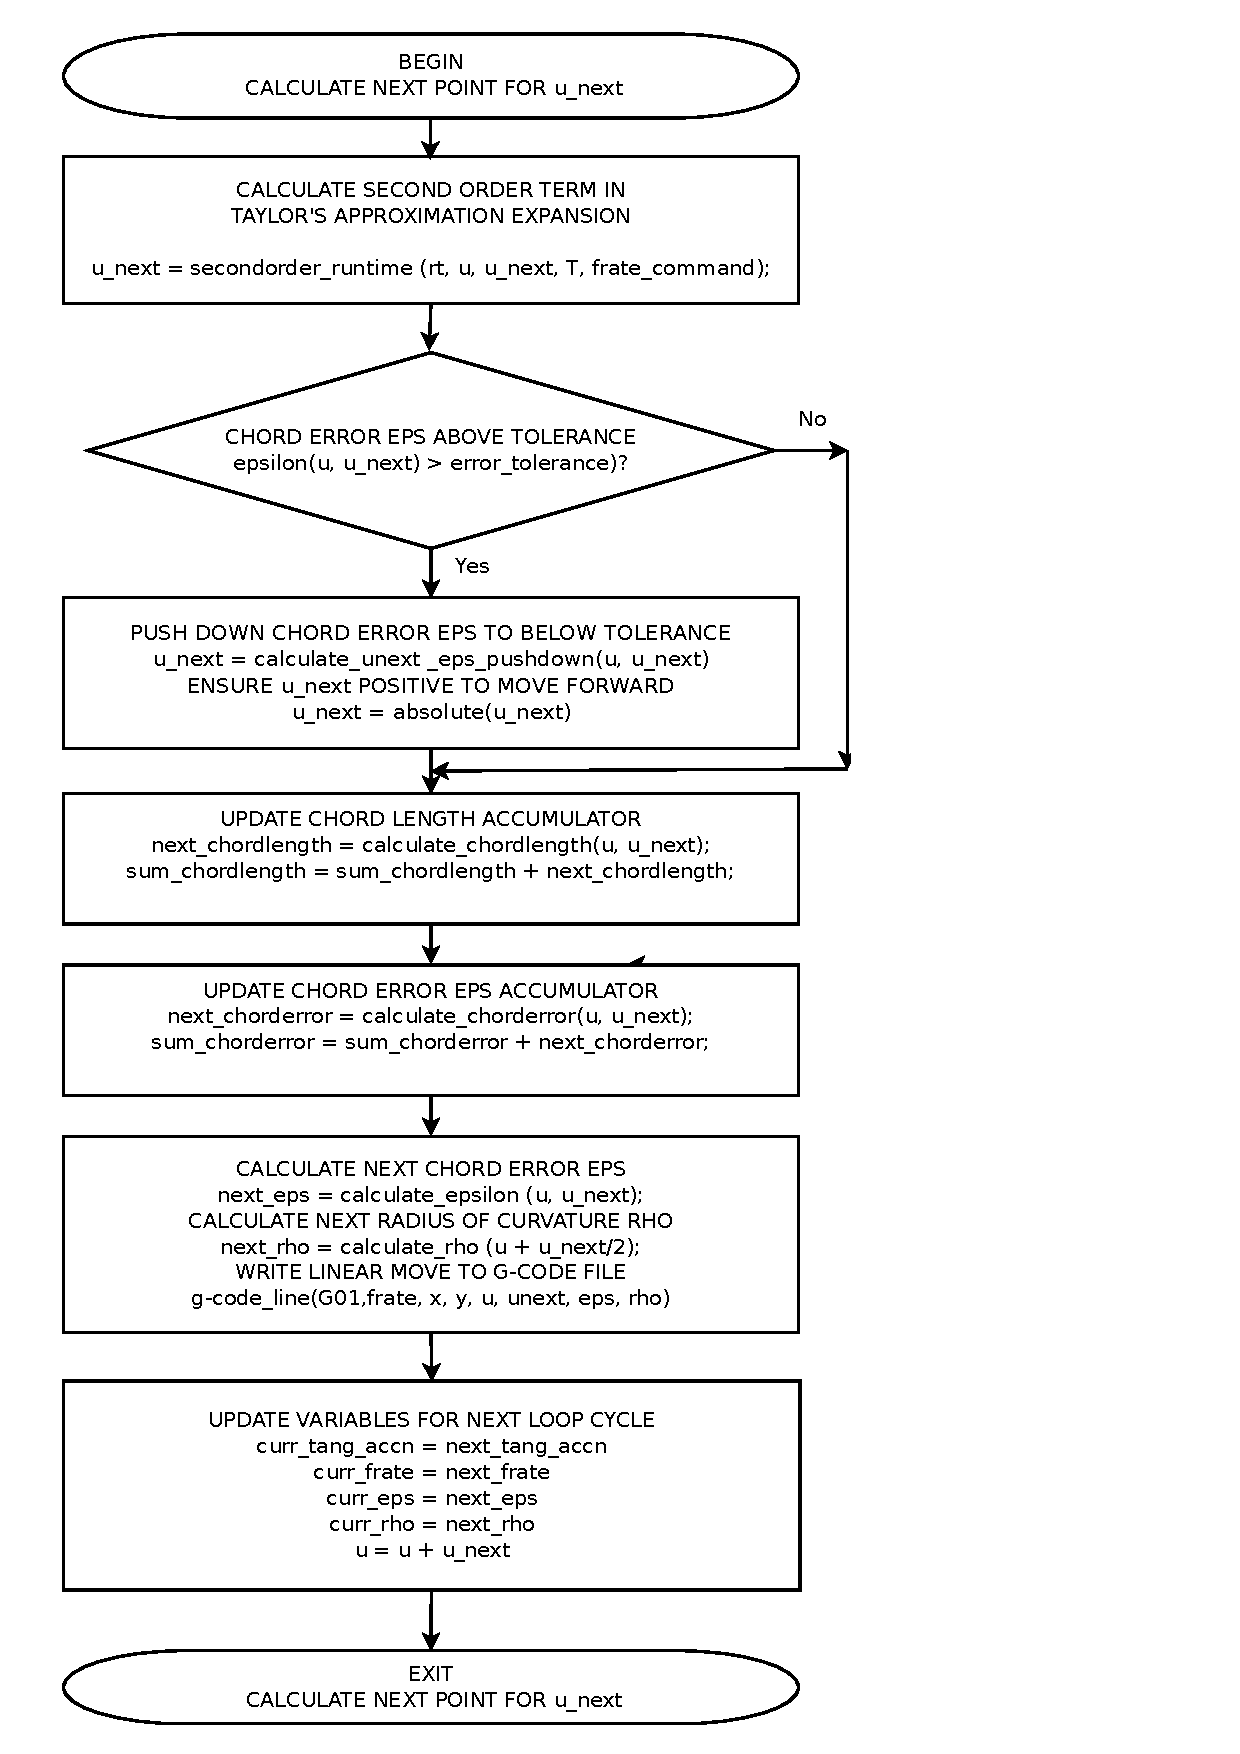
\includegraphics[width=1.10\textwidth,]{Images/Chap3/04-Calculate-u-next-flowchart.pdf} 
\end{figure}

%% =============================================
\clearpage
\pagebreak

\begin{figure}
	\caption{Flowchart Calculate u\_next(u) with eps pushdown}
	\label{05-Calculate-u-next-eps-pushdown-flowchart.pdf}
	%%\centering
	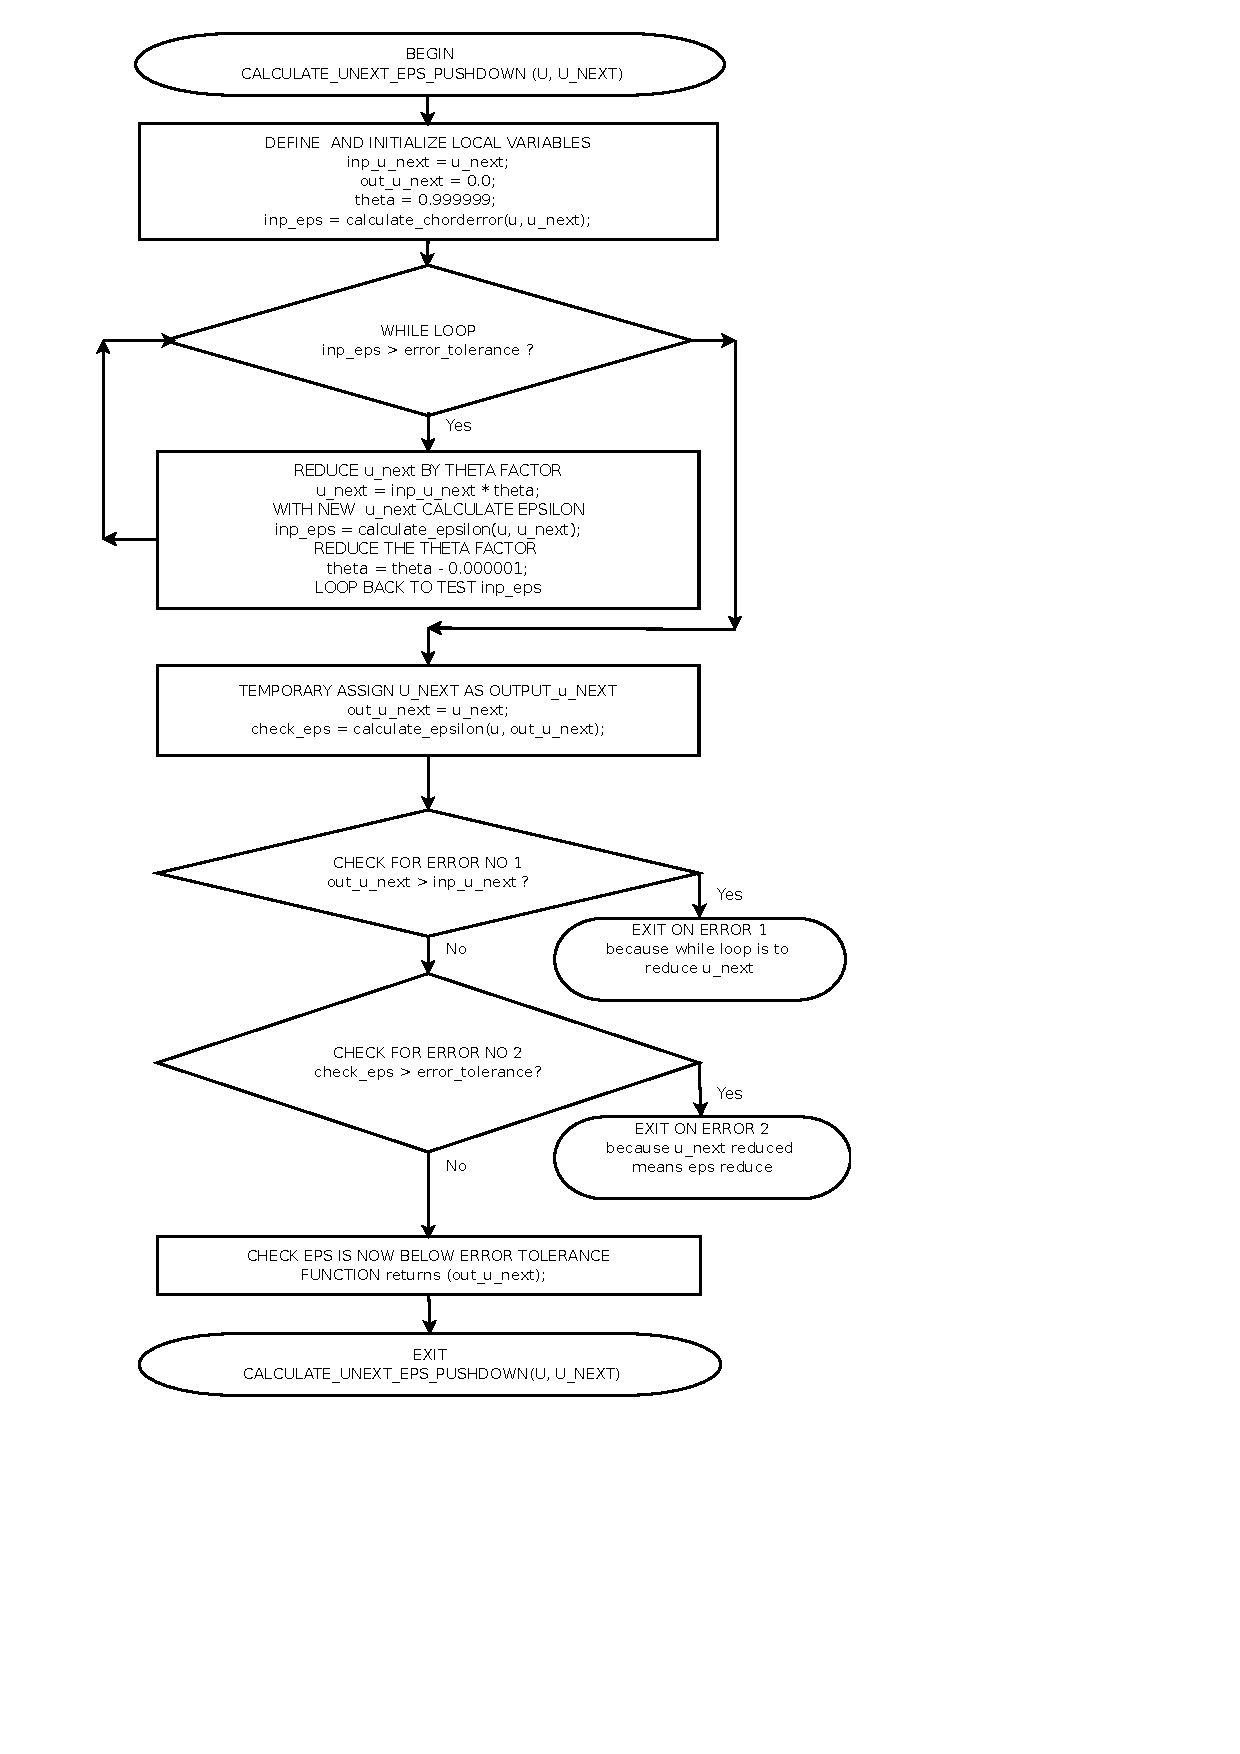
\includegraphics[width=1.40\textwidth,]{Images/Chap3/05-Calculate-u-next-eps-pushdown-flowchart.pdf} 
\end{figure}

%% FALLING FEEDRATE FLOWCHART
%% =============================================
\clearpage
\pagebreak

%% PERFECT INCLUDE PDF IN LATEX (AS ONE FULL PAGE)
\begin{figure}
	\caption{Flowchart of Feedrate Falling S-Curve}
	\label{03-Feedrate-Falling-Region-flowchart.pdf}
	\centering
	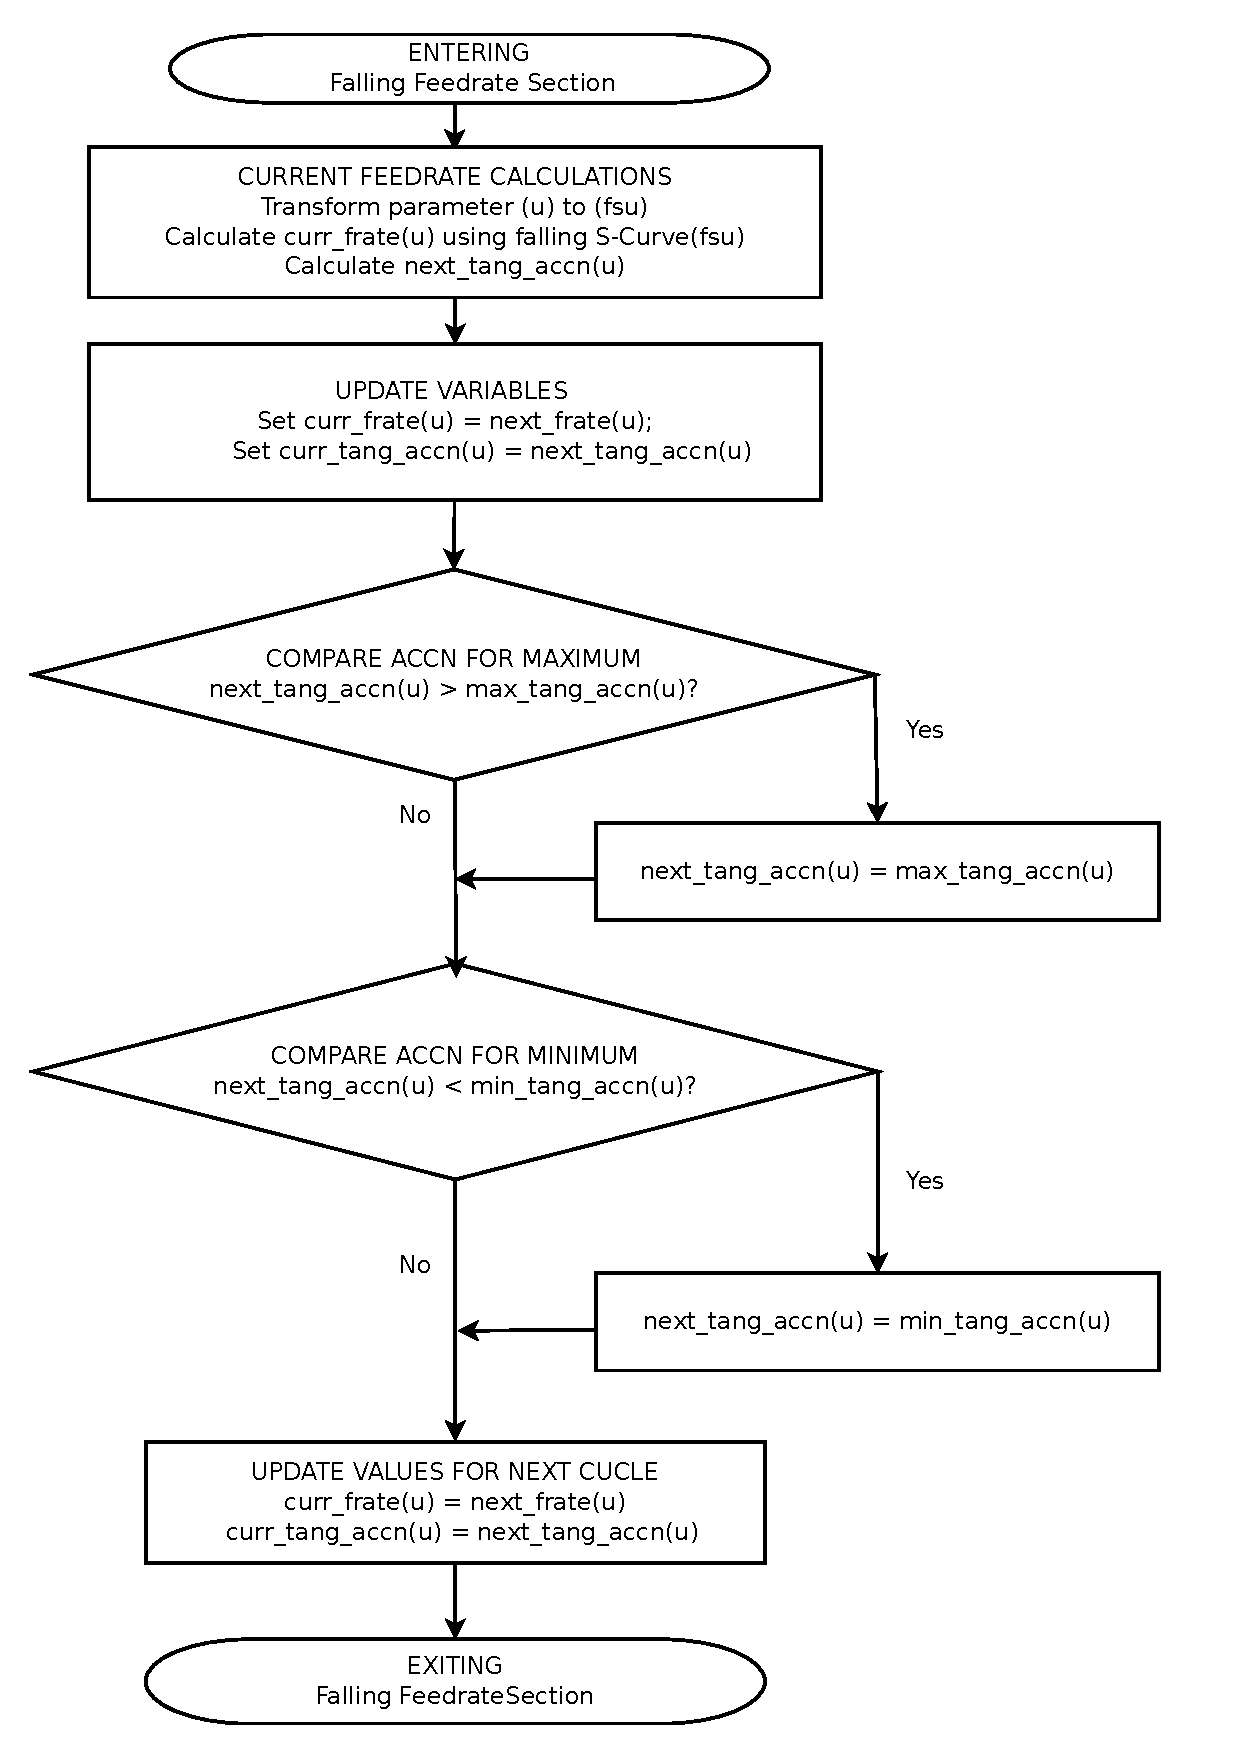
\includegraphics[width=1.10\textwidth,]{Images/Chap3/03-Feedrate-Falling-Region-flowchart.pdf} 
\end{figure}
%% 
%% ==============================================


% ======================================================
\clearpage
\pagebreak
\section{Feedrate falling S-curve}

The feedrate must not fall abruptly to zero. A smooth feedrate fall is required to ensure machine stability. The S-shaped curve below was selected for the fall of the current running feedrate to zero. \\

\[ curr\_frate(fsu) = 1 - \frac{curr\_frate\_limit(fsu)} { \Bigg( 1 + e^{(-fsu*fshape1)} \Bigg) ^{fshape2} }  \] \\

\noindent
where the applicable variable range is \\
$fsu\_start\_fall$ $\le$ $fsu$ $\le$ $fsu\_end\_fall$\\

\noindent
The linear parameter transformation from $u$ to $fsu$ is as follows:\\
$fsu$ = $fm*u$ + $fkonst$ \\

To ensure smoothness of the falling feedrate curves, simulations were conducted to determine the best values of the parameters.These variables are user specified.\\


\begin{table}[!ht]
	\begin{center}
		\caption{Falling S-curve parameters}
		\label{Falling-S-curve-parameters}	
		\begin{tabular}{ p{3.0cm} p{2.0cm} p{8.0cm}}
			\hline	
			fsu\_start\_fall & = 0.95  & beginning of falling S-curve \nonumber \\
			fsu\_end\_fall   & = 1.00  & end of falling S-curve \nonumber \\
			fshape1          & = 5.00  & S-curve smoothness shaping factor \nonumber \\
			fshape2          & = 8.00  & S-curve smoothness shaping factor \nonumber \\
			fsu1             & = 0.00  & start of u linear transformation\nonumber \\
			fsu2             & = 3.00  & end of u linear transformation \nonumber \\
			fm               & = calc  & slope calculated for each parametric curve \nonumber \\
			fkonst			 & = calc  & constant calculated for each parametric curve \nonumber \\ 
			fsu              & = calc  & transformed variable in the rising S-curve \nonumber \\
			\hline
		\end{tabular}
	\end{center}
\end{table}

%% ==============================================
\clearpage
\pagebreak

\section{Acceleration constraint lambda safety factor}

\begin{table}[ht]
	\begin{center}
		\begin{tabular}{ p{14.0cm} }
			\caption{Acceleration safety factor (lambda)}
			\begin{eqnarray}
            lamda  & = & user\_select\_safety\_factor(0.0 to 1.0)     \nonumber \\
%%	alphaVel(u) & = &  \Bigg | \frac { \Bigg (\odv{x(u)}{u} \Bigg) } { \sqrt { \Bigg( {\odv{x(u)}{u}} \Bigg )^{2} +  \Bigg ( {\odv{y(u)}{u}} \Bigg )^{2} } }  \Bigg |  \nonumber \\
%%	betaVel(u)  & = &  \Bigg | \frac { \Bigg (\odv{y(u)}{u} \Bigg) } { \sqrt { \Bigg( {\odv{x(u)}{u}} \Bigg )^{2} +  \Bigg ( {\odv{y(u)}{u}} \Bigg )^{2} } }  \Bigg |  \nonumber \\
			C & = & \sqrt {\frac{lamda*rho*xAcc_{max}} { \Bigg |(betaVel) \Bigg |} } \nonumber \\
			D & = & \sqrt {\frac{lamda*rho*yAcc_{max}} { \Bigg |(alphaVel)\Bigg |} } \nonumber \\
			fratelimit\_4 & = & minimum (C, D) \nonumber
			\end{eqnarray}
		\end{tabular}
	\end{center}
\end{table}

The $fratelimit\_4$ is about acceleration confinement within a (min, max) range of permissible accelerations. It is dependent on the combined dynamical and geometrical constraints. The dynamical machine constraints are in the maximum allowable axial accelerations of the machine as covered by $xAcc_{max}$ and $yAcc_{max}$. The geometrical constraints are in $alphaVel(u)$, $betaVel(u)$ and $rho(u)$, since $u$ changes along the curve these geometrical values also change. \\

The choice for the value of lambda, the safety factor for containment of acceleration, makes a big impact on the occurrence of jerks (jitters) in the feedrate. The values of 0.10, 0.18, 0.20 and 0.50 for lambda were tested for the algorithm runs to eliminate the jerks. A lower value of lambda will eliminate jerks but will reduce the feedrate significantly. The results for the threshold value for lamda is provided in Chapter 4 at reference link [\ref{chap4-Determination of acceptablel lamda}].

%% =============================================
\clearpage
\pagebreak

\section{Four(4) Algorithm Performance Metrics}

\noindent
There are four(4) metrics to assess the overall algorithm performance in this work. The first three terms are ratios while last term is
a percentage measure of the difference.

\begin{enumerate}
	\item SCE/TIP : This is the ratio of total sum-chord-error divided by the total number of interpolated points.  
	\item SCE/SCL : This is the ratio of total sum-chord-error divided by the total sum-chord-length.
	\item SAA/SCL : This is the ratio of the sum-arc-areas divided by the total sum-chord-length.
	\item 100(SAL-SCL)/SAL : This is the ratio of the difference between the sum-arc-length and the sum-chord-length, divided by the sum-arc	length and multiplied by 100 to represent it in percentage form. 
\end{enumerate} 

The calculation for the individual arc-length (AL) is provided in section [\ref{chap3-Arc-Length Approximate calculation}]. The calculation for the individual chord-length (CL) is provided in section [\ref{chap3-Chord-Length Exact calculation}]. The calculation for the individual arc-theta (AT) is provided in section [\ref{chap3-Arc-Theta Approximate calculation}]. The calculation for the individual arc-area (AA) is provided in section [\ref{chap3-Arc-Area Approximate calculation}]. \\

Consider these two(2) important terms. The term NAL(u) is the next-arc-length or length of the arc calculated by the algorithm from point u to the point u + (u next). Similarly, NCL(u) is the next-chord-length or length of the chord calculated by the algorithm from point u to the point u + (u next).\\

By definition, the sum-arc-length SAL(u), is the cumulative sum of NAL(u) from NAL(0.00) to NAL(u), where u is incremented by (u-next) in each step. Similarly, the sum-chord-length SCL(u), is the cumulative sum of NCL(u) from NCL(0.00) to NCL(u). Generally, we have the following definition of terms in this work.

\clearpage
\pagebreak

\begin{table}[ht]
%% \begin{center}

%% IMPORTANT TO SCALEBOX BELOW
\scalebox{0.90}{

\begin{tabular}{ p{16.0cm} }
\caption{Definitions of SAL(u), SCL(u), SAT(u), SAA(u) and SCE(u)}
\begin{eqnarray}
SAL(u) & = & \sum_{k=0.00}^{u}NAL(k) \nonumber  \\
SCL(u) & = & \sum_{k=0.00}^{u}NCL(k) \nonumber  \\
SAT(u) & = & \sum_{k=0.00}^{u}NAT(k) \nonumber  \\
SAA(u) & = & \sum_{k=0.00}^{u}NAA(k) \nonumber  \\
SCE(u) & = & \sum_{k=0.00}^{u}NCE(k) \nonumber  
\end{eqnarray}
\end{tabular}
%% \end{center}
}   %% IMPORTANT FOR SCALEBOX CLOSING
\end{table}


%% ===================================
\begin{table}[ht]
%% \begin{center}

%% IMPORTANT TO SCALEBOX BELOW
\scalebox{0.90}{

\begin{tabular}{ p{16.0cm} }
\caption{Definitions of Total SAL, Total SCL, Total SAT, Total SAA, and Total SCE}
\begin{eqnarray}
Total\_SAL & = & \sum_{k = 0.00}^{k = 1.00}NAL(k) \nonumber  \\
Total\_SCL & = & \sum_{k = 0.00}^{k = 1.00}NCL(k) \nonumber  \\
Total\_SAT & = & \sum_{k = 0.00}^{k = 1.00}NAT(k) \nonumber  \\
Total\_SAA & = & \sum_{k = 0.00}^{k = 1.00}NAA(k) \nonumber  \\
Total\_SCE & = & \sum_{k = 0.00}^{k = 1.00}NCE(k) \nonumber  
\end{eqnarray}
\end{tabular}
%% \end{center}

}   %% IMPORTANT FOR SCALEBOX CLOSING
\end{table}

\noindent
Note that the variable k is discrete and non-uniform. In fact, the successive values of k are exactly the successive values of u, generated by the interpolation algorithm, that is, while simultaneously constraining chord-error and running feedrate. \\

\noindent
Saying it is a straightforward manner, the values of k are exactly the values of the interpolated points u. That is the reason for k being non-uniformly spaced. Finding this k points is in fact, the main objective of the work in this thesis.

%% =============================================
\clearpage
\pagebreak

\subsection{Arc-Length Approximate calculation}
\label{chap3-Arc-Length Approximate calculation}

\begin{figure}
\caption    {Calculation for the Circle Arc-Length}
\label{chap3-Calculation for the Circle Arc-Length}
\centering
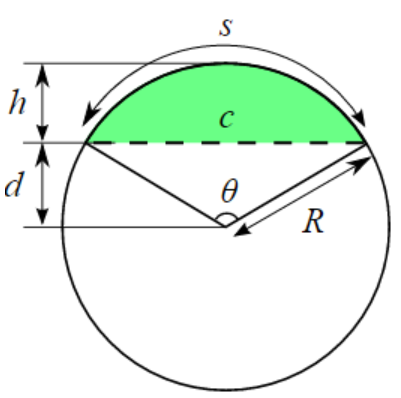
\includegraphics[width=0.60\textwidth,]{Chap3/images/Calculation-of-arc-segment-of-a-circle.png} 
\end{figure}

\noindent
The first-order approximation for the calculation of the arc-length $AL(u, u\_next)$ segment of a generic curve with equation C(x(u), y(u)), where x(u) and y(u) are known is given by:\\

\noindent
$ AL(u, u\_next) = (u\_next) * \sqrt{ {{\Bigg ( \odv{x}{u} \Bigg )^{2}} + {\Bigg ( \odv{y}{u} \Bigg )^{2} }} }  $  \\

\lstset{backgroundcolor=\color{white}, basicstyle=\linespread{1.00}\footnotesize, frame={topline, bottomline, leftline, rightline}}	
\begin{lstlisting}[caption={Implementation for Approximate Arc-Length Calculation}, label=lst-Implementation for Approximate Arc-Length Calculation]

// ==================================================================
double fxn_calc_arc_length(double u, double u_next)
// ==================================================================
{
  // LOCAL VARIABLES
  double arc_length = 0.0;
	
  // GEOMETRIC CALCULATION ARC LENGTH OF PARAMETRIC CURVES
  double dx_du = fxn_cvel_x(u);
  double dy_du = fxn_cvel_y(u);
  double sumsquare = (dx_du)*(dx_du) + (dy_du)*(dy_du);
  double arc_length0 = (u_next)*sqrt(sumsquare);
  arc_length = fabs(arc_length0);

  return (arc_length);
}
\end{lstlisting}


%% =============================================
\clearpage
\pagebreak

\subsection{Chord-Length Exact calculation}
\label{chap3-Chord-Length Exact calculation}

\noindent
The exact calculation for the chord-length $CL(u, u\_next)$ of a generic curve with equation C(x(u), y(u)), between two points on the curve at (x1, y1) and (x2, y2) is given by:\\

\noindent
$ CL(u, u\_next) = \sqrt{ \Bigg (x2-x1 \Bigg)^{2} + \Bigg (y2-y1 \Bigg )^{2}  } $ \\

\lstset{backgroundcolor=\color{white}, basicstyle=\linespread{1.00}\footnotesize, frame={topline, bottomline, leftline, rightline}}	
\begin{lstlisting}[caption={Implementation of Exact Chord-length Calculation}, label=lst-Implementation of Exact Chord-length Calculation]

// ==================================================================
double fxn_calc_chordlength_use_paramcurve (double u, double u_next)
// ==================================================================
{
  double chordlength;
  double x1, x2, y1, y2;
	
  // Use param curve and geometry
  x1 = fxn_cpos_x (u);
  y1 = fxn_cpos_y (u);
  x2 = fxn_cpos_x(u+u_next);
  y2 = fxn_cpos_y(u+u_next);
	
  // Pythagoras theorem for a right angled triangle
  chordlength = fabs(sqrt(pow((x2-x1), 2.0) + pow((y2-y1), 2.0)));
	
  return (chordlength); 
}
\end{lstlisting}


%% =============================================
\clearpage
\pagebreak

\subsection{Arc-Theta Approximate calculation}
\label{chap3-Arc-Theta Approximate calculation}

\noindent
The equation for the approximate arc-theta requires chord-length CL, and the radius of curvature rho values. The equation  used in this calculation is based on website reference [\href{https://www.engineersedge.com/math/circular_segment_equation_and_calculator__13796.htm}{circular\_segment\_equation\_and\_calculator}]. \\

$Arc\_Theta(CL, R) =  (2)*sin^{-1}(CL/2R) $\\

\noindent 
where R = approximately Radius of Curvature rho, and the chord-length CL is calculated from a previous equation.\\ 


\lstset{backgroundcolor=\color{white}, basicstyle=\linespread{1.00}\footnotesize, frame={topline, bottomline, leftline, rightline}}	
\begin{lstlisting}[caption={Implementation of Approximate Arc-Theta Calculation}, label=Implementation of Approximate Arc-Theta Calculation]

// ==================================================================
double fxn_calc_arc_theta(double u, double chord_length, double rho)
// ===================================================================
{
  double arc_theta = 0.0; 
  double arg_arcsine = chord_length/(2.0*rho);
	
  if ( (arg_arcsine < -1.0) || (arg_arcsine > +1.0) ) 
  {
    printf("ERROR: Angle_theta is out of range [-1.0 : +1.0] \n");
    printf("Value of angle arg_arcsine = %.12e \n", arg_arcsine );
    exit (1);
  } else {
    arc_theta = 2.0*asin(arg_arcsine);
  }
	
  return(arc_theta);
}
\end{lstlisting}

%% =============================================
\clearpage
\pagebreak

\subsection{Arc-Area Approximate calculation}
\label{chap3-Arc-Area Approximate calculation}


\noindent
The arc-area is the area bounded by the chord and the arc-segment. The equation for the approximate arc-area requires the radius of curvature rho and the angle theta in radians subtended by the arc segment. The equation  used in this calculation is based on website reference [\href{https://www.engineersedge.com/math/circular_segment_equation_and_calculator__13796.htm}{circular\_segment\_equation\_and\_calculator}]. \\

$Arc\_Area(R, theta) = (R^{2}/2)*(theta - sin(theta)) $\\

\noindent 
where R = approximately Radius of Curvature rho, and the subtended angle theta is in radians.\\ 


\lstset{backgroundcolor=\color{white}, basicstyle=\linespread{1.00}\footnotesize, frame={topline, bottomline, leftline, rightline}}	
\begin{lstlisting}[caption={Implementation of Approximate Arc-Area Calculation}, label=Implementation of Approximate Arc-Area Calculation]
	
// ==================================================================
double fxn_calc_arc_area(double u, double chord_length, double rho)
// ===================================================================
{
	double arc_area = 0.0;
	
	// GET VALUE OF ARC-THETA FROM PREVIOUS FUNCTION
	double arc_theta = fxn_calc_arc_theta(u, chord_length, rho);
	double DIFF = arc_theta - sin (arc_theta);

	// CALC ARC AREA
	arc_area = (rho*rho) * (DIFF)/2;
	
	return(arc_area);
}
\end{lstlisting}

%% =============================================

%% ==================================
\clearpage
\pagebreak

\section{Software engineering practice}
\label{sec-Software engineering practice}


The premise for the conduct of this thesis is to have a software design that is structured, fully functionalized and modularized. The use of GNAT Studio 2021 as the Integrated Development Environment (IDE) allows a combination of C, C++ and Ada code to be compiled together into a single executable. Ada is known for safe and secure codes and includes its own realtime library. \\

In general, software code implementations must not only run correctly, but must also run efficiently. Therefore, design of the codes must follow good software engineering practices. This thesis is under the category of mechatronics and systems design, so correct software codes is an important and critical part of the work. \\

The algorithm design must be highly structured, functionalized and modularized. This practice makes program execution flow readable and understandable. The resulting flowcharts will provide easy error tracing, adaptations, and additions of new functionality. \\
	
For example, inexperienced software programmers forget the simple rule that every time a function returns from a call, then all values of local variables are wiped out from memory. This requires that local variables be saved globally before the called function returns. This is a basic computing principle. \\
	
Technically, when a function executes, it may add some of its local state data to the top of the stack; when the function exits it is responsible for removing that data from the stack. In other words, since the stack memory of a function gets deallocated after the function returns, there is no guarantee that the value stored in those area will stay the same. References: \cite{Wikipedia:2023A} and \cite{Chen:2023}. \\
	
Another issue is the concept of zero in computing machines. In codes using floating-point representation of real numbers, any number below machine-epsilon (macheps), is treated as zero by the machine for addition and subtraction operations. Machine-epsilon is actually a very small but non-zero number, that varies from machine to machine. In the work conducted in this document at reference [App\ref{app4-Calculation of machine epsilon C code}], the machine-epsilon (macheps) for 64-bit double type was found to be  $2.22(10)^{-16}$. This means an algorithm check for addition or subtraction by zero is actually a check of addition or subtraction of very small non-zero numbers with values below machine-epsilon. Reference: \cite{Wikipedia:2023B}. \\
	
The side-effect phenomena in computing is another important issue. In computer science, an operation, function or expression is said to have a side effect if it modifies some state variable value(s) outside its local environment. This means, there are additional effects other than its primary effect of just returning a value to the caller of the operation. Because the algorithm in this work uses many global and local variables, it can be difficult to track changes and side-effects, that is, if the algorithm is not designed properly. Reference: \cite{Wikipedia:2023C}. \\
	
A decision operation (diamond flowchart symbol) must only have two outputs, True of False. It is a mistake, in fact a serious error not to have two branches as outputs. The algorithm must be designed to exit when there is an error at any point in its execution because all subsequent (downstream) calculations can be considered erroneous (useless) due to this upstream error. \\ 
	
Inclusion of error trapping functions is vital in any processing code. The algorithm in this work, for example, traps errors when $u\_next$ repeatedly stays at "zero" in five(5) consecutive loops in Taylor's expansion calculation. This means the interpolation step does not move forward to the next point. This is caused by the effect of machine epsilon. The "zero" here does not mean real zero, but is the computer machine-epsilon, the smallest non-zero value the computer can represent. Any value below this machine-epsilon is treated as zero for additions and subtractions by the computer. \\ 
	
Algorithm verification through accounting is the term used in this work to check that all calculations tally to the correct expected total value. As an example, the algorithm was built to check that the histogram total sum value (of interpolated points) tallies with the total number of interpolated points. Similarly, the histogram total sum value (of points above feedrate limit, and points below feedrate limit) tallies with the total number of interpolated points. In the same manner, the histogram total sum value (of points where chord-errors are all below tolerance) tallies with the total number of interpolated points.\\
	
In this work, the algorithm verification conducted above proves the achievement in simultaneously constraining chord-error and feedrates, thus meeting the objective of the interpolation algorithm.   \\


%% ==============================================================
%% MOVED FROM RESULTS CHAPTER
%% ==============================================================

\section{Design of Algorithm Codes}

\subsection{Algorithm Text Reports}

Every combination of the set (curve type, feedrate command FC and lamda safety factor) made as input to the algorithm will generate a summary report.\\

As examples, two(2) snippets of the summary report in this work for the Teardrop and Butterfly curves are provided in Listing [\ref{snp-Teardrop Algorithm Summary Output}] and Listing [\ref{snp-Butterfly Algorithm Summary Output}], respectively.\\

The snippet only shows Report No. 09 specifically on Algorithm Execution Statistics. There are eight(8) prior reports in the full report summary list for each execution run.\\




%% ========================================================
\clearpage
\pagebreak
%% \begin{landscape}

%% INPUT FROM FILE
%% \lstinputlisting[⟨key=value list⟩]{⟨file name⟩}
%% typesets the stand alone source code file as a displayed listing.
%% \lstset{backgroundcolor=\color{white}, basicstyle=\linespread{0.9}\scriptsize, frame={topline, bottomline, leftline, rightline}}

\lstset{backgroundcolor=\color{white}, basicstyle=\linespread{0.90}\footnotesize, frame={topline, bottomline, leftline, rightline}}	
\begin{lstlisting}[caption={Snippet of Teardrop Algorithm Summary Output}, label=snp-Teardrop Algorithm Summary Output]	
	
FC20-L0.18-A28-TEARDROP (REPORT NO. 09) ALGORITHM EXECUTION STATISTICS 	
	
TEARDROP TOTAL-INTERPOLATED-POINTS          	7.599000000000E+03
TEARDROP SUM-CHORD-ERROR-(mm)               	7.140807162860E-03
TEARDROP SUM-CHORD-ERROR/TOT-INTERPOL-PNTS  	9.398272128007E-07
	
TEARDROP SUM-ARC-LENGTH-(mm)                	1.018418663504E+02
TEARDROP SUM-CHORD-LENGTH-(mm)              	1.018418655699E+02
TEARDROP DIFF-ARC-LENGTH-CHORD-LENGTH-(mm)  	7.805327442156E-07
TEARDROP PCNT-DIFF-ARC-CHORD-LENGTH         	7.664163788301E-07
	
TEARDROP SUM-CHORD-ERROR/SUM-CHORD-LENGTH   	7.011661778683E-05
	
TEARDROP SUM-ARC-THETA-(rad)                	4.712268805770E+00
TEARDROP SUM-ARC-AREA-(mm2)                 	6.182290957317E-05
	
TEARDROP SUM-ARC-AREA/SUM-CHORD-LENGTH      	7.011661778683E-05
	
TEARDROP AVG-CHORD-ERROR-(mm)               	9.398272128007E-07
TEARDROP AVG-ARC-LENGTH-(mm)                	1.340377288107E-02
TEARDROP AVG-CHORD-LENGTH-(mm)              	1.340377277834E-02
TEARDROP AVG-ARC-THETA-(rad)                	6.201985793327E-04
TEARDROP AVG-ARC-AREA-(mm2)                 	8.136734610840E-09
	
2023-10-05 10:43:45	Program run duration   19.907344569 seconds. 
	
\end{lstlisting}
%% \end{landscape}

\lstset{backgroundcolor=\color{white}, basicstyle=\linespread{0.90}\footnotesize, frame={topline, bottomline, leftline, rightline}}	
\begin{lstlisting}[caption={Snippet of Butterfly Algorithm Summary Output}, label=snp-Butterfly Algorithm Summary Output]	
	
FC30-L0.18-A28-BUTTERFLY (REPORT NO. 09) ALGORITHM EXECUTION STATISTICS 		
	
BUTTERFLY TOTAL-INTERPOLATED-POINTS          	1.234300000000E+04	
BUTTERFLY SUM-CHORD-ERROR-(mm)               	4.846582536157E-03	
BUTTERFLY SUM-CHORD-ERROR/TOT-INTERPOL-PNTS  	3.926902071104E-07	
	
BUTTERFLY SUM-ARC-LENGTH-(mm)                	3.560730284349E+02	
BUTTERFLY SUM-CHORD-LENGTH-(mm)              	3.560727930088E+02	
BUTTERFLY DIFF-ARC-LENGTH-CHORD-LENGTH-(mm)  	2.354260789161E-04	
BUTTERFLY PCNT-DIFF-ARC-CHORD-LENGTH         	6.611735799000E-05	
	
BUTTERFLY SUM-CHORD-ERROR/SUM-CHORD-LENGTH   	1.361121273884E-05	
	
BUTTERFLY SUM-ARC-THETA-(rad)                	2.211618559661E+01	
BUTTERFLY SUM-ARC-AREA-(mm2)                 	1.298932073590E-03	
	
BUTTERFLY SUM-ARC-AREA/SUM-CHORD-LENGTH      	1.361121273884E-05	
	
BUTTERFLY AVG-CHORD-ERROR-(mm)               	3.926902071104E-07	
BUTTERFLY AVG-ARC-LENGTH-(mm)                	2.885051275603E-02	
BUTTERFLY AVG-CHORD-LENGTH-(mm)              	2.885049368083E-02	
BUTTERFLY AVG-ARC-THETA-(rad)                	1.791945032946E-03	
BUTTERFLY AVG-ARC-AREA-(mm2)                 	1.052448609294E-07	
	
2023-10-05 15:57:25	Program run duration    8.667691811 seconds. 
	
\end{lstlisting}
%% \end{landscape}

% ===================================
\clearpage
\pagebreak'
\subsection{Algorithm Functional Organization}


The functional organization of software codes for the realtime interpolation algorithm in this work is shown in Figure [\ref{img-Algorithm-Functional-Components}]. \\

The main algorithm in $src/algo$ comprises a series of seven(7) calculation modules, with the last module being the writing of RS272/NGC G-Code. The name of each code file is self-explanatory.\\

The $src/common$ and $src/cpp-codes$ folders are for local and imported code utilities commonly shared among the modules. The Integrated Development Environment (IDE) used in this work is capable of compiling C, C++ and Ada source codes combined into a single binary executable.\\

The $src/curves$ folder is where the ten(10) parametric curves in this work are located. The $src/files$ folder is the directory where all source codes to generate data and reports are located. This includes code to generate the G-Code file.\\

The $src/parallel\_pci$ and $src/parallel\_usb$ are the directories containing interface codes for the hardware parallel port on the computer. The former hardware is for PCI Parallel Card interface, while the later hardware is for USB-to-Parallel device interface.  \\

The $src/pthread$ folder is for multi-threading codes (C/C++ and Ada) while the $src/realtime$ folder is for Ada and C/C++ codes that implement realtime libraries. Note that Ada has its own built-in $Ada.Realtime$ library.\\

Multi-threading in Ada is called $Tasking$. Multi-threading for the algorithm in this project was tested successfully, however the overall execution is too slow and so was abandoned. It was found that the creation and destruction of new threads for runtime parameter at every u-loop is time-consuming. With that, the serial and sequential mode of processing was adopted for the algorithm.\\ 

The $src/reports$ folder is the storage location for all finished data and report files. The names of the files are meaningful like:
\singlespacing
\noindent $data\_calc\_frate\_limit.txt$,\\ 
$data\_calc\_intgrl\_error.txt$, \\
$data\_calc\_arclength\_chordlength.txt$,\\
$data\_calc\_tang\_accn.txt$,\\
$data\_calc\_time\_lookahead.txt$,\\ 
$data\_calc\_u\_next.txt$, \\
$data\_calc\_raw\_curve.txt$,
\doublespacing

\noindent and many more. Depending on the total number of interpolated points for the run, each file size typically ranges between one to 10 megabytes.\\ 

The $obj$ folder is the location of intermediate files during compilation, binding and linking. It is a system controlled folder and contains binary and semi-binary files. A snippet of the process of compilation, binding and linking is shown in Listing [\ref{snp-Snippet of Algorithm Compilation Binding and Linking}].\\

Finally, the $exec$ folder is where the single binary executable for the algorithm in this work is located. This binary executable is less than 100 kilobytes, and is considered very small.

% ===================================
\clearpage
\pagebreak'

%% NOTE: Limit is 0.55 of width	

\begin{figure}
	%% \centering
	\caption  {Algorithm-Functional-Components}
	\label{img-Algorithm-Functional-Components}
	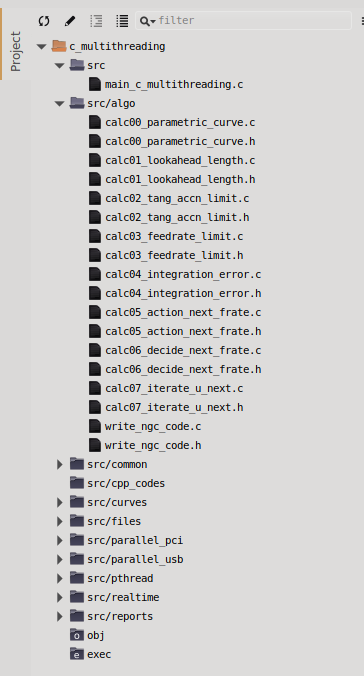
\includegraphics[width=0.55\textwidth]{Chap4/BW-Image-Algorithm-Functional-Components.png} 
\end{figure}

% ===================================
\clearpage
\pagebreak'

%% \begin{landscape}

%% INPUT FROM FILE
%% \lstinputlisting[⟨key=value list⟩]{⟨file name⟩}
%% typesets the stand alone source code file as a displayed listing.
%% \lstset{backgroundcolor=\color{white}, basicstyle=\linespread{0.9}\scriptsize, frame={topline, bottomline, leftline, rightline}}

\lstset{backgroundcolor=\color{white}, basicstyle=\linespread{0.92}\footnotesize, frame={topline, bottomline, leftline, rightline}}	
\begin{lstlisting}[caption={Snippet of Algorithm Compilation, Binding and Linking}, label=snp-Snippet of Algorithm Compilation Binding and Linking]	
	
gprbuild -d -P/home/wruslan/WRY-UMP-Thesis/
/Teadrop-FC20-Lamda018-Algo28-Codes/c_multithreading.gpr -s -k
	
Compile
[C]            main_c_multithreading.c
[C]            c_position.c
[C]            c_velocity.c
[C]            c_accelern.c
[C]            calc03_feedrate_limit.c
[C]            calc00_parametric_curve.c
[C]            calc06_decide_next_frate.c
[C]            calc07_iterate_u_next.c
[C]            write_ngc_code.c
[C]            calc05_action_next_frate.c
[C]            calc01_lookahead_length.c
[C]            calc02_tang_accn_limit.c
[C]            calc04_integration_error.c
[C]            preempt_rt.c
[C]            main_usb-to-parallel-port.c
[C]            usb_parallel_port.c
[C]            pci_parallel_port.c
[C]            c_report_01.c
[C]            test_threads_01.c
[C]            c_min_max_int_dbl_in_array.c
[C]            c_dtstamp.c
[C]            c_random_int_dbl.c
[C]            c_parallel_port.c
Link
[archive]      libc_multithreading.a
[index]        libc_multithreading.a
[link]         main_c_multithreading.c
[2023-10-10 11:06:29] process terminated successfully, time: 02.36s
	
\end{lstlisting}
%% \end{landscape}
%% ===================================


\clearpage
\pagebreak
\subsection{Algorithm and runtime parameters}\label{tab-Algorithm and runtime parameters}

The configuration of parameters in the realtime interpolation algorithm in this work is categorized into 3 sections, namely, the machine limits, the software runtime values, and the user specified runtime parameters. It is provided in Table [\ref{Algorithm and runtime parameters}] below. \\

\begin{table}[ht]
	%% \begin{center}
	\caption{Algorithm and runtime parameters}
	\label  {Algorithm and runtime parameters}
	%% IMPORTANT TO SCALEBOX BELOW
	\scalebox{0.90}{
		
		%% START COPY AND PASTE BELOW HERE
		%% FROM \begin{tabular} UNTIL \end{tabular)
		
		\begin{tabular}{ p{0.5cm} p{4.0cm} p{1.25cm} p{1.25cm} p{7.50cm} }
			\hline
			&                     &                 &       &     \\
			& MACHINE LIMITS      & VALUE  & UNIT   & DESCRIPTION \\
			%%	&                     &        &        &     \\
			1	&  x\_Vel\_max        & 30.0   & mm/s   & X-axis maximum velocity \\
			2	&  y\_Vel\_max        & 30.0   & mm/s   & Y-axis maximum velocity \\
			3	&  x\_Acc\_max        & 30.0   & mm/s2  & X-axis maximum acceleration\\
			4	&  y\_Acc\_max        & 30.0   & mm/s2  & y-axis maximum acceleration\\
			5	&  Jerk\_max          & 200.0  & mm/s2  & Maximum allowable jerk\\
			&                     &        &       &     \\
			& RUNTIME VALUES      &        &       &     \\
			%%	&                     &        &       &     \\
			1   & u\_end\_rise        &  0.05  & nil   & Rising S-curve range (0.0 .. 0.05)\\
			2   & rshape1             &  5.00  & nil   & Sigmoid curve rise shaping factor 1\\
			3   & rshape2             &  8.00  & nil   & Sigmoid curve rise shaping factor 2\\
			4   & u\_start\_fall      &  0.95  & nil   & Falling S-curve range (0.95 .. 1.00)\\   
			5   & fshape1             &  5.00  & nil   & Sigmoid curve fall shaping factor 1)\\
			6   & fshape2             &  8.00  & nil   & Sigmoid curve fall shaping factor 2)\\
			7	& T\_interpol         & 0.001  & s     & Interpolation time (period) \\
			&                     &        &       & 1 millisecond per step. \\
			8	& Error\_tol          & 1E-6   & mm    & Chord-error tolerance for  \\
			&                     &        &       & maximum allowable chord-error. \\
			9   & ngc\_scale          & 1.0    & nil   & RS274/NGC G-code scaling factor \\
			10	& ngc\_feedrate\_min  & 3.0    & mm/s  & Minimum NGC feedrate setting for\\
			&                     &        &       & startup and shutdown of CNC machine.\\
			11	& PI constant used    & PI     & nil   & PI = 3.14159\_26535\_89793\_238 precision\\
			&                     &        &       & at 18 decimal digits (from internet)\\
			&                     &        &       &     \\
			& RUN SPECIFIED       &Example &       &     \\
			%%	&                     &        &       &     \\
			1   & Curve selection     & AstEpi & nil   & Curve selected for algorithm to execute. \\
			&                     &        &       & Ten(10) different choices for this work. \\
			2   & Feedrate Command FC &  20.0  & mm/s  & Maximum feedrate set that should not \\
			&                     &        &       & be exceeded. For example: 10, 20, 30. \\
			3   & Lamda safety factor &  0.18  & nil   & Acceleration limit safety factor. \\
			&                     &        &       & A number between (0.0 .. 1.0) \\
			&                     &        &       &     
		\end{tabular}
		
		%% END COPY AND PASTE		
		
	}   %% IMPORTANT FOR SCALEBOX CLOSING
	\hrule
\end{table}

Note that the Feedrate Command (FC) is the value of the running feedrate that the user wants if it is following a straight line without any constraints. This is the user preferred feedrate. \\

The Feedrate Command is one of the four (4) components that determine the feedrate limit. The feedrate limit is dynamic, changes as parameter u changes, and is the minimum value among the four(4) components. The Feedrate Command is a user selected system constant. In the algorithm, the running feedrate is "forced and adjusted" to be as close to the feedrate limit throughout the parameter range.

%% ==============================================================
%% ==============================================================

\clearpage
\pagebreak

\section{Working environment setup}

The four(4) computing machines in this work comprise HP-Laptop-01, HP-Laptop-02, HP-Desktop-01 and HP-Desktop-02. The two laptops are identical in hardware specifications (HP brand, 8-CPU cores, 16 GB Memory, 1.5 TB SSD storage and so on). Similarly, the two desktops are also identical in hardware specifications (HP brand, 8-CPU cores, 16 GB Memory, 1.5 TB SSD storage and so on). The complete hardware specifications for the computing machines in this work are provided in Table [\ref{chap3-System Hardware Specifications}].\\

All four(4) computing machines are configured in a 3-way multiboot operating system. The user can select any one of the following operating systems: Linux Debian 10 Buster, Linux Ubuntu 20.04 LTS, or Microsoft Windows 10 Professional. The details are provided in Table [\ref{chap3-Operating Systems}].\\ 

All four(4) computing machines are installed with the same application software. This means the software installed are clones of each other. The details are provided in Table [\ref{chap3-Programming Software Languages}] for the programming languages, Table [\ref{chap3-Reporting Software Applications}] for the reporting software, and Table [\ref{chap3-Specialized Software Applications}] for the specialized software applications.\\

In the table for specialized software applications, the LinuxCNC-Axis software is the primary application to drive the CNC machine for all the G-codes generated in this work. The Panaterm application is used to communicate and monitor the status of the proprietary CNC-Servo drives responsible for control ofbthe CNC machine. The oscilloscope software, available for both Linux and Windows versions, are used to simultaneously trace 8-channels of digital or analog electrical signals. The CuteCom application is an RS232 serial communication software used drive and monitor serial signals in this work, including snooping, that is, a third party listening to RS232 serial communication between two serial devices. The DAQNavi Control Application is for Advantech products like PCIE-1884 DAQ card, and for user interface development using Qt6 C/C++ codes.\\    




%% ==============================================
\clearpage
\pagebreak

\section{System Hardware Environment}

\begin{table}[ht]
%%	\begin{center}
\caption{System Hardware Specifications}
\label{chap3-System Hardware Specifications}
\begin{tabular}{p{0.5cm} p{4.30cm} p{9.2cm} }
\hline	
\textbf{No} & \textbf{Category}   &    \textbf{Specification Description}\\
\hline
	&                       &    \\
1   &   HP-Laptop-01        & Model Hewlett-Packard, HP EliteBook 8570w \\
2	&   HP-Laptop-02        & Intel(R) Core(TM) i7-3630QM CPU @ 2.40GHz \\
	&                       & CPU Two Quad(4) cores, 64 bits, with 8 threads\\
	&                       & DDR3 16 GB System board memory, 1600 MHz clock\\
	&                       & System Caches: L1 32 KB, L2 256 KB, L3 6 MB\\
	&                       & SDDs: 1TB and 512GB Kingston Solid State Drives\\ 
	&                       & Display NVIDIA Corporation GK107GLM \\ 		
	&                       & GPU NVIDIA Corporation [Quadro K1000M]\\ 		
	&                       & Parallel parport0 PC-style 0x378 (0x778), irq 5\\
	&                       &    \\  
3   &	HP-Desktop-01       & Model Hewlett Packard EliteDesk 800 G1 TWR   \\
4   &	HP-Desktop-02       & Intel(R) Core(TM) i7-4790 CPU @ 3.60GHz \\  
	&                       & CPU Two Quad(4) cores, 64 bits, with 8 threads\\
	&                       & DDR3 18 GB System board memory, 1600 MHz clock\\
	&                       & System Caches: L1 256 KB, L2 1 MB, L3 8 MB\\
	&                       & SDDs: 1TB and 512GB Kingston Solid State Drives\\
	&                       & Display NVIDIA Corporation GK208 64bits 33Mhz\\ 
	&                       & GPU NVIDIA Corporation [GeForce GT 710B]\\         
	&                       & PCI parport0: PC-style 0xd100, irq 16 \\
	&                       & [PCSPP,TRISTATE]\\
	&                       & Advantech PCIE-1884 Signal processing card 32 bits\\
    &                       & \\
\hline
\end{tabular}

%% \hrule
%% \hline
%% \end{center}
\end{table}



%% ===============================================
\clearpage
\pagebreak
\section{Software Environment}

\subsection{Operating System}

\begin{table}[ht]
\caption{Operating Systems}
\label{chap3-Operating Systems}

\begin{tabular}{p{0.5cm} p{4.30cm} p{9.2cm} }
\hline	
\textbf{No} & \textbf{Category}   &    \textbf{Specification Description}\\
\hline
  &                       &    \\
1 & Ubuntu 20.04.6 LTS    & HP-Desktop-01 and 02, HP-Laptop-01 and 02\\
  &                       & Codename: focal, LSB version core-11.1 \\                   
  &                       & Kernel: linux-5.15.0-83-lowlatency \\
  &                       & SMP PREEMPT (2023) x86\_64 \\
  &                       & Preemptive Realtime OS, Symmetric Multi-Processor\\
  &                       &    \\  
2 &	Debian GNU/Linux 10   & HP-Desktop-01 and 02, HP-Laptop-01 and 02\\
  &                       & Codename: Buster   \\
  &                       & Kernel: 4.19.0-25-rt-amd64 x86\_64 GNU/Linux \\
  &                       & SMP PREEMPT RT Debian 4.19.289-2 (20230808) \\  
  &                       & Preemptive Realtime OS, Symmetric Multi-Processor\\
  &                       &    \\
3 & MS Windows 10 Pro     & HP-Desktop-01 and 02, HP-Laptop-01 and 02 \\
  &                       &    \\
  &                       &    \\
\hline
\end{tabular}  
\end{table}

%% ========================================  

\subsection{Programming Software Languages}  
  
\begin{table}[ht]
\caption{Programming Software Languages}
\label{chap3-Programming Software Languages}

\begin{tabular}{p{0.5cm} p{4.30cm} p{9.2cm} }
\hline	
\textbf{No} & \textbf{Category}   &    \textbf{Specification Description}\\
\hline
  &                       &    \\                    
1 &	C/C++, Ada            & GNAT Studio Community 2021 (20210423) \\ 
  &                       & GNAT 9.4.0 targeting x86\_64-linux-gnu   \\  
  &                       & SPARK Community 2021 (20210519)   \\    
  &                       &    \\
2  & GUI for C/C++         & Qt Creator 10.0.1 x86-64 \\
  &                       & Based on Qt 6.4.3 (GCC 10.3.1 20210422)   \\
  &                       & Built on May 04, 2023   \\
  &                       &    \\
3 &	Python                & Python 2.7.18 (Jul 1 2022), [GCC 9.4.0] on linux2\\
  &                       & Python 3.8.10 (May 26 2023), [GCC 9.4.0] on linux3\\
  &                       &    \\
4 &	Julia/Atom            & Julia Version 1.9.0 (2023-05-07)/Atom 1.58.0 x64 \\  
  &                       & \\
\hline
\end{tabular}  
\end{table}


%% ============================================
\clearpage
\pagebreak

\subsection{Reporting Software Applications}

\begin{table}[ht]
\caption{Reporting Software Applications}
\label{chap3-Reporting Software Applications}
	
\begin{tabular}{p{0.5cm} p{4.30cm} p{9.2cm} }
\hline	
\textbf{No} & \textbf{Category}   &    \textbf{Specification Description}\\
\hline
1 &	TeXstudio             & TeXstudio 3.0.1 (git n/a)  \\
  &                       & Using Qt Version 5.12.8, compiled with Qt 5.12.8 R   \\
  &                       &    \\
2 &	LibreOffice Suite     & Version: 6.4.7.2, Build ID: 1:6.4.7-0ubuntu0.20.04.8 \\
  &                       & CPU threads: 8; OS: Linux 5.15; UI VCL: gtk3; \\
  &                       &    \\ 
3 & Master PDF Editor     & Version 5, Build 5.7.60, 64 bit, (2021)  \\
  &                       & GCC: 5.3.1, GLIBC: 2.17, Qt: 5.9.5, SANE: 1.0.25  \\ 	
  &                       &    \\
4 &	Dia diagram editor    & Dia Version 0.97 + git (2011)\\
  &                       &    \\
5 & Gnuplot               & Gnuplot Version 5.2 patchlevel 8 (2019-12-01) \\ 
\hline
\end{tabular}
\end{table}

\subsection{Specialized Software Applications}

\begin{table}[ht]
\caption{Specialized Software Applications}
\label{chap3-Specialized Software Applications}
	
\begin{tabular}{p{0.5cm} p{4.30cm} p{9.2cm} }
\hline	
\textbf{No} & \textbf{Category}   &    \textbf{Specification Description}\\
\hline
1 &	CNC Control App       & LinuxCNC/Axis ver. 2.8.0 (2016)\\ 
  &                       & on Linux Debian 10 (Buster)  \\
  &                       &    \\
2 &	CNC Monitoring  App   & Panaterm version 4.5 (Panasonic)\\
  &                       & on Microsoft Windows 10 Pro \\
  &                       & \\
3 & Oscilloscope App      & Bitscope Digital Storage Oscilloscope (DSO) \\
  &                       & Linux - Version 2.8 Intel x86-64-bit \\ 	
  &                       & Windows - Version 2.8 Intel x86-64-bit \\   
  &                       &   \\ 
4 & Serial Communication  & CuteCom graphical serial terminal (RS232) \\ 
  & RS232 Snooper circuit & Linux GUI Version  0.30.3 (2015) \\
  &                       & Windows GUI Version  0.30.3 (2015)\\
  &                       &     \\
5 & DAQNavi Control App   & Advantech PCIE-1884 Data Acquisition Card \\ 
  &                       & Linux GUI Version  4.0.8.0 64-bit \\
  &                       & Windows GUI Version  4.0.8.0 64-bit\\  
 \hline
\end{tabular}
\end{table}

%% ==============================================
%% ==============================================
\clearpage
\pagebreak
\section{CNC System Setup}

The image of the CNC machine used in this work is shown in Figure [\ref{CNC-Research-Machine-3-Axis.jpg}]. The next Figure [	\ref{CNC-Research-Machine-3-Sets-Servo-Drives.jpg}] shows the three(3) Panasonic AC-Servo-Drives for the x, y, and z axes motions of the CNC machine. For this machine, the z-axis is used to move the pen tool up and down.\\ 

The next image shown in landscape mode in Figure [\ref{BHN-Validation-in-LinuxCNC-Axis-Screenshot.png}] illustrates the operations of the LinuxCNC-Axis software in driving the CNC machine to draw the diagram on its screen. The diagram to be drawn is represented by a G-code, a snippet of the code is provided in Listing [\ref{Link-to-Arabic-Calligraphy}]. \\

The image of the CNC system environment is shown in Figure [\ref{THE-FRONT-END-WhatsAppImage.jpeg}] and Figure [\ref{THE-BACK-END-WhatsAppImage.jpeg}]. \textit{Note: The images will be changed later.}\\


The overview of the CNC system environment is shown in Figure [\ref{Overview-CNC-system-environment.pdf}]. The multiplexed monitoring of the CNC Panaterm controller is shown in Figure [\ref{CNC-system-Panaterm-controller.pdf}]. The wiring diagram connections for parallel port, CNC servos and PCIE-1884-card is shown in Figure [\ref{Parport-CNC-servo-PCIE-1884-wiring-diagram.pdf}]. The snooper circuit for a third party computer to listen to RS232 serial communications between two devices is provided in Figure 	[\ref{RS232-Snooper-Circuit.pdf}].\\



%% ==============================================
\clearpage
\pagebreak

\begin{figure}
	\centering
	\includegraphics[width=1.00\textwidth]{Images/Chap4/CNC/CNC-Research-Machine-3-Axis.jpg} 
	\caption{The prototype 3-axis CNC research machine}
	\label{CNC-Research-Machine-3-Axis.jpg}
\end{figure}

\begin{figure}
	\centering
	\includegraphics[width=1.00\textwidth]{Images/Chap4/CNC/CNC-Research-Machine-3-Sets-Servo-Drives.jpg} 
	\caption{The 3-sets AC servo drivers for the CNC research machine}
	\label{CNC-Research-Machine-3-Sets-Servo-Drives.jpg}
\end{figure}

%% LANDSCAPE LINUXCNC AXIS
%% ==============================
\clearpage
\pagebreak
\begin{landscape}
	\begin{figure}
	\caption{Validation of G-code using LinuxCNC Axis software}	
	\label{BHN-Validation-in-LinuxCNC-Axis-Screenshot.png}		
	\centering
	\includegraphics[width=1.70\textwidth]{Chap2/Images/BHN-Validation-in-LinuxCNC-Axis-Screenshot.png} 
	\end{figure}
\end{landscape}


% LISTING
%% ==============================
\clearpage
\pagebreak
\begin{landscape}
	
%% INPUT FROM FILE
%% \lstinputlisting[⟨key=value list⟩]{⟨file name⟩}
%% typesets the stand alone source code file as a displayed listing.
%% \lstset{backgroundcolor=\color{white}, basicstyle=\linespread{0.9}\scriptsize, frame={topline, bottomline, leftline, rightline}}
	
\lstset{backgroundcolor=\color{white}, basicstyle=\linespread{0.92}\footnotesize, frame={topline, bottomline, leftline, rightline}}	
\begin{lstlisting}[caption={G-code snippet for Arabic calligraphy}, label=Link-to-Arabic-Calligraphy]	
(Header)
(Generated by gcodetools from Inkscape.) 
(Using default header. To add your own header create file "header" in the output dir.)
M3
(Header end.)
G21 (All units in mm)
(Start cutting path id: path11762)
(Change tool to Default tool)
G00 Z5.000000
G00 X235.600000 Y35.100000
G01 Z1.000000 F100.0(Penetrate)
G03 X213.627800 Y25.129879 Z1.000000 I60.683117 J-162.930013 F400.000000
G03 X212.000000 Y22.400000 Z1.000000 I1.475151 J-2.729879
G03 X212.577899 Y21.936846 Z1.000000 I0.474545 J-0.000000
G03 X218.800000 Y23.900000 Z1.000000 I-8.264838 J37.036796
G02 X225.555826 Y26.585083 Z1.000000 I199.253827 J-491.492772
G02 X241.000000 Y32.500000 Z1.000000 I527.010173 J-1352.932266
G03 X257.708311 Y40.036826 Z1.000000 I-45.059557 J122.180722
G03 X259.000000 Y42.200000 Z1.000000 I-1.165476 J2.163174
G03 X258.293460 Y42.724778 Z1.000000 I-0.548158 J0.000000
G03 X235.600000 Y35.100000 Z1.000000 I111.496791 J-369.428872
G01 X235.600000 Y35.100000 Z1.000000
G00 Z5.000000
....
\end{lstlisting}
%% } %% END SCALEBOX

\end{landscape}
	
%% FRONT END ENVIRONMENT
%% ==============================
\clearpage
\pagebreak

\begin{landscape}
\begin{figure}
%%	\centering
\caption{The front end environment of the system}
\includegraphics[width=1.60\textwidth]{Image0/THE-FRONT-END-WhatsAppImage.jpeg} 
\label{THE-FRONT-END-WhatsAppImage.jpeg}
\end{figure}
\end{landscape}

%% BACK END ENVIRONMENT
%% ==============================
%%\clearpage
%%\pagebreak
%%\begin{landscape}
%%	\begin{figure}
	%%	\centering
%%		\caption{TEMPORARY - The back end environment of the system}
%%		\includegraphics[width=1.60\textwidth]{Image0/THE-BACK-END-WhatsAppImage.jpeg} 
%%		\label{THE-BACK-END-WhatsAppImage.jpeg}
%%	\end{figure}
%% \end{landscape}


%% ==============================
\clearpage
\pagebreak

\begin{figure}
	\caption{Overview CNC system menvironment}
	\label{Overview-CNC-system-environment.pdf}
	\includegraphics[width=1.00\textwidth]{Chap3/work-setup/Overview-CNC-system-environment.pdf} 
\end{figure}


\begin{figure}
	\caption{CNC-system-Panaterm-controller}
	\label{CNC-system-Panaterm-controller.pdf}
	\includegraphics[width=1.00\textwidth]{Chap3/work-setup/CNC-system-Panaterm-controller.pdf} 
\end{figure}


\begin{figure}
	\caption{Parport-CNC-servo-PCIE-1884-wiring-diagram}
	\label{Parport-CNC-servo-PCIE-1884-wiring-diagram.pdf}
	\includegraphics[width=1.00\textwidth]{Chap3/work-setup/Parport-CNC-servo-PCIE-1884-wiring-diagram.pdf} 
\end{figure}

\begin{figure}
	\caption{RS232 Snooper Circuit}
	\label{RS232-Snooper-Circuit.pdf}
	\includegraphics[width=1.00\textwidth]{Chap3/work-setup/RS232-Snooper-Circuit.pdf} 
\end{figure}


%%% ==============================
%%% END METHODOLOGY CHAPTER

\chapter{RESULTS AND DISCUSSIONS}


\section{CHAPTER ORGANIZATION}


\subsection{Result comparisons with Published Reference Paper}

This section discusses the results of this work in comparison to the published reference paper by \cite{Zhong-etal:2018}, titled "A realtime interpolator for parametric curves". The results in this work showed similar patterns and comparable values to the published referenced results. The comparisons cover the feedrate variations along the curve, the velocity profiles of the x and y axes motions, the current running feedrate profile against the feedrate-limit,  and the acceleration profile.  These results spanned the entire traversal along the parametric curve. 
  

\subsection{Algorithm Executions}

This section discusses the total number of algorithm executions, history of algorithm revisions, selection of an illustrative curve among the ten(10) parametric curves, acceleration jitters, and determination of the acceptable or nominal value of the acceleration safety factor lamda to avoid acceleration jitters.  

\subsection{Teardrop Curve for Illustration}

This section describes the characteristics of the Teardrop curve, and the basic reasons for making the Teardrop curve as an illustration curve. The rest of the nine(9) curves are described in comparison to the Teardrop curve.

\subsection{Results of Teardrop curve}

This section discusses the full outputs of the Teardrop curve resulting from the algorithm execution. Similar outputs for the rest of the nine(9) curves are provided in their respective appendices.\\

These illustrative outputs cover, for example, the direction of travel for the curve, the radius of curvature rho(u), the first and second-order terms in Taylor's expansion, the chord-error absolute constraint, the running feedrate absolute constraint, the four(4) components of the feedrate limit, histogram distribution of interpolated points, starting and ending feedrate profiles, color coded running feedrates and many more.

\subsection{Notable Results for Rest of Curves}

This section discusses specific aspects of the execution results worthy of further clarification. Four(4) special cases were considered. Results of the Circle and Ellipse curves that can be used as a means of validation and verification of algorithm performance were highlighted. Results that look abnormal but are correct need to be explained. This cover negative results for the difference (SAL-SCL) in the Teardrop curve, and machine epsilon problems for the SnaHyp curve. 

\subsection{Overall Execution Results}

This section presents the algorithm execution summary results for all of the ten(10) parametric curves studied in this work. The discussions include the Feedrate Command (FC) and the Lamda safety factor (LSF), algorithm validation and verification (V \& V), LinuxCNC-Axis simulation run validation (SRV), real run validation on the CNC machine (RRV), and algorithm performance measures.\\

The performance measures cover algorithm generated variables like total interpolated points (TIP), total sum-arc-length (SAL), total sum-chord-length (SCL), total sum-chord-error (SCE), total sum-arc-theta (SAT), and total sum-arc-area (SAA). \\

The four(4) assessment metrics for algorithm performance are: (SCE/TIP), (SCE/SCL), (SAA/SCL) and 100*(SAL-SCL)/SAL. The first three terms are ratios while last term is a percentage measure of the difference.


\subsection{Summary of Results Chapter}
 
This section summarizes the important findings in this chapter.\\

\noindent
\textbf{IMPORTANT NOTE}: Some data tables and graphs are displayed in landscape mode, when it is not possible in portrait mode. The landscape mode facilitates presentation of multiple plots side by side, including and especially wide data tables. This mode helps comprehension, visualization and comparison of information.

% ========================================================
\clearpage
\pagebreak
%% \begin{landscape} 

\section{COMPARISONS AGAINST PUBLISHED PAPER}

\subsection{Result comparisons with Published Reference Paper}

It is important to note that the comparisons of results in this work can only be made against the Teardrop parametric curve in the referenced paper by \cite{Zhong-etal:2018}, because this work uses the same parametric equation. And it must also be reminded that the single interpolation algorithm designed and developed in this work is to cater ten(10) different parametric curves of various features, shapes and dimensions, not just the one simple Teardrop curve. \\

The computational algorithms are also different between this work and the published paper. The overall algorithm in this work is considered simpler (not complicated branching flow), highly structured (for example, one-way-in and one-way-out for every computing unit), and therefore easy to understand and maintain. In addition, this algorithm strictly enforces complete and simultaneous non-violation of chord-error and feedrate-limit constraints. The results is absolute success when applied to all ten(10) different parametric curves. \\   

For the above reasons, it cannot be said that the algorithm is an-apple-to-apple comparison with that of the published paper, even for the identical Teardrop curve. Obviously, the computation techniques are different. However, the common theme is that both are "interpolation algorithms", meaning given a current point on the parametric curve, find the next point for the move on the curve. These are the reasons it was stated that the results in this work showed similar patterns and comparable values. The comparisons are described in the next section.

%% ===========================================================
\clearpage
\pagebreak
%% \begin{landscape} 

\subsection{Display comparison results}

\noindent The four(4) comparisons for the Teardrop curve cover : \\
\noindent 
(1) Feedrate variations along the curve shown in Fig[\ref{img-Feedrate variations along the curve}].\\
(2) Velocity profiles of the x and y axes motions shown in Fig[\ref{img-Comparisons velocity profiles of the x and y axes motions}].\\
(3) Running feedrate profile against the feedrate-limit shown in Fig[\ref{img-Running feedrate profile against the feedrate-limit}].\\  
(4) Acceleration profile containment shown in Fig[\ref{img-Acceleration profile containment}].


\subsection{Discussion on comparative results}

\noindent It is important to note that This-Work (PhD thesis) provides results that are similar and comparable to the work produced in the Reference-Paper. This comparison is only applicable to the Teardrop because both adopted the same exact equation for the parametric curve. The four(4) figures for comparison in the next section are provided in landscape mode. The legend colors of the curves displayed in the figures were made identical for easy visual comparison. \\

\noindent
In Fig[\ref{img-Feedrate variations along the curve}], the feedrate variations in the interpolation are similar and comparable. The generally lower feedrate values in This-Work as the (x, y) position point moves along the Teardrop trajectory is due to both the simultaneous absolute constraints on chord-error (epsilon) and non-violation of the machine feedrate limit. In the Reference-Paper, there is a push-up of the running feedrate, which causes an increase in chord-length, thereby an increase in chord-error. In the Reference-Paper there is no specific mention of absolutely restricting the chord-error for each interpolation point in parameter (u).\\ 

\noindent
Also in Fig[\ref{img-Feedrate variations along the curve}], the different colors refer to the magnitudes of the feedrate (mm/s), which varies from point-to-point on the parametric curve. In this work, the colors transition smoothly following the color spectrum. There is no jumping of colors. The direction of travel of the (x, y) point is starting from the apex going counter-clockwise. \\

\noindent 
In Fig[\ref{img-Comparisons velocity profiles of the x and y axes motions}], the velocity profiles of the x and y axes motions are also similar and comparable. However, the number of interpolated points in This-Work (7599 points) is higher than the Reference-Paper. See the x-axis for the runtime in seconds. Each cycle of interpolated points is set the same for both works, that is, at 0.001 (s) or one millisecond. This makes the completion time for the interpolation algorithm in This-Work as 7.6 seconds, while that for the Reference-Paper as about 6.3 seconds.\\   

\noindent
In Fig[\ref{img-Running feedrate profile against the feedrate-limit}], the actual running feedrate (velocity) almost overlaps with the machine feedrate limit calculated by the algorithm. The feedrate determination is one of the most important and difficult computation to handle. It is a combined effect of both dynamical and kinematical constraints which varies among different CNC machines. \\

\noindent 
Also in Fig[\ref{img-Running feedrate profile against the feedrate-limit}], with the exception of the initial rise and final fall of the actual feedrates, the middle section shows that in both the Reference-Paper and This-Work, the actual running feedrate follows exactly the value of feedrate limit calculated by the algorithm. In this middle region, it is almost overlapping. The actual initial rise and final fall of the actual feedrates are user-selected S-curves. In This-Work, the initial S-curve-rise region is set at (u = 0.00 to 0.05) and the final S-curve-fall region is set at (u = 0.95 to 1.00). In the Reference-Paper, the characteristics of both S-curve-rise and S-curve-fall regions are not specifically mentioned. \\

\noindent
In Fig[\ref{img-Acceleration profile containment}], the actual running tangential acceleration is constrained within the minimum and maximum accelerations in both the Reference-Paper and This-Work results. The acceleration values are not identical but comparable. The feature for acceleration constraints (min, max) is similar. In This-Work, the value of lambda (acceleration safety factor) was selected to be 0.18, chosen to eliminate acceleration jitters that causes machine velocity jerks. This number 0.18 is good when applied to all ten(10) different parametric curves covered in This-Work. In the Reference-Paper, it was only mentioned that lambda should be within (0.00 and 1.00). The determination of acceptable lambda (acceleration safety factor) is discussed in detail in Section [\ref{chap4-Determination of acceptablel lamda}] in this chapter.  

%% \end{landscape}
%% ===========================================================
\clearpage
\pagebreak
\begin{landscape} 
	
\begin{figure}
	\centering
	\caption  {Feedrate variations along the curve}
	\label{img-Feedrate variations along the curve}
	\includegraphics[width= 1.40\textwidth]{Chap4/Comparisons/01-Comparison-Feedrate-Variations-Along-The-Curve.png} 
\end{figure}		

\noindent
\textbf{Equivalent legend}: Reference-Paper (left figure) versus This-Work (right figure)\\

\end{landscape}
% ========================================================
\clearpage
\pagebreak
\begin{landscape} 

\begin{figure}
	\centering
	\caption  {Comparisons velocity profiles of the x and y axes motions}
	\label{img-Comparisons velocity profiles of the x and y axes motions}
	\includegraphics[width= 1.40\textwidth]{Chap4/Comparisons/02-Comparison-Feedrate-Profiles-X-and-Y-Axes.png} 
\end{figure}		

\noindent
\textbf{Equivalent legend}: Reference-Paper (left figure) versus This-Work (right figure)\\
F = curr-frate (Current running feedrate)\\
X = x-frate (X-axis feedrate)\\
Y = y-frate (Y-axis feedrate)\\
Time = rtime (Runtime)\\

\end{landscape}


%% ===========================================================
\clearpage
\pagebreak
\begin{landscape} 
	
\begin{figure}
\centering
\caption  {Running feedrate profile against the feedrate-limit}
\label{img-Running feedrate profile against the feedrate-limit}
\includegraphics[width= 1.50\textwidth]{Chap4/Comparisons/03-Comparison-Running-feedrate-profile-against-the-feedrate-limit.png} 
\end{figure}		
	
\noindent
\textbf{Equivalent legend}: Reference-Paper (left figure) versus This-Work (right figure)\\


\end{landscape}

%% ===========================================================
\clearpage
\pagebreak
\begin{landscape} 
	
\begin{figure}
\centering
\caption  {Acceleration profile containment}
\label{img-Acceleration profile containment}
\includegraphics[width= 1.30\textwidth]{Chap4/Comparisons/04-Comparison-Acceleration-profile-containment.png} 
\end{figure}		
	
\noindent
\textbf{Equivalent legend}: Reference-Paper (left figure) versus This-Work (right figure)\\


\end{landscape}
% ========================================================
% ========================================================
\clearpage
\pagebreak

\subsection{Validation of Teardrop curve on CNC machine}

\noindent The following are runtime characteristics of the Teardrop curve computed by the interpolation algorithm for FC20, the Feedrate Command and Lamda = 0.18, the acceleration safety factor. 

\begin{enumerate}
\item Width  (mm)   = 28.8
\item Height (mm)   = 37.5
\item Total interpolated points   = 7599
\item Sum Total arc   length (mm) = 101.8418663504 
\item Sum Total chord-length (mm) = 101.8418655699 
\item Sum Total chord-error  (mm) = 0.007140807163 
\item Average chord-length   (mm) = 0.013403772778 	
\end{enumerate}

\noindent Notice that the CNC machine moves about 7600 incremental steps to cover the distance of 102 mm (about 4 inches) of the total Teardrop curve. This step move is very small indeed, maintaining chord-error below 1 (nm) nanometer and speed (feedrate) below the feedrate limit throughout the entire curve. The average chord-length or linear move per step is 0.0134 (mm). It is quite remarkable that the simple CNC machine is capable of the very small increments. \\

\noindent A snapshot of the CNC machine in operation is shown in Fig[\ref{img-Execution of Teardrop Curve on CNC Machine}] on the next page. A simple pen is used to trace the trajectory of the Teardrop curve. The results for the completed execution of the Teardrop curve is shown next in Fig[\ref{img-Results of Teardrop Curve CNC Machine execution}]. The run was repeated twice for confirmation of correctness.

%% ===========================================================
\clearpage
\pagebreak
%% \begin{landscape} 

%% Left: 01-Teardrop-run-on-CNC-Machine.png
%% Right: 02-Teardrop-run-on-CNC-Machine.png	

\begin{figure}
	\centering
	\caption  {Execution of Teardrop Curve on CNC Machine}
	\label{img-Execution of Teardrop Curve on CNC Machine}
	\includegraphics[width=0.60\textwidth]{Chap4/Validation/01-Teardrop-run-on-CNC-Machine.png} 
\end{figure}	

\begin{figure}
	\centering
	\caption  {Results of Teardrop Curve CNC Machine execution - ruler (cm)}
	\label{img-Results of Teardrop Curve CNC Machine execution}
	\includegraphics[width=0.70\textwidth]{Chap4/Validation/02-Teardrop-run-on-CNC-Machine.png} 
\end{figure}

	
%% \end{landscape}
% ========================================================
% ========================================================
\clearpage
\pagebreak
%% \begin{landscape} 


\section{ALGORITHM EXECUTIONS}

\subsection{Total algorithm executions}

In this work we have executed the algorithm for ten(10) different curves, four(4) different feedrate commands (FC 10, 20, 30, 40), and four(4) different Lamda safety factors (Lamda 0.10, 0.18, 0.20, 0.50). This combination makes the total number of algorithm executions at 160. For each execution, 3 different input parameters are required, that is, curve type selected, feedrate command FC, and Lamda safety factor. \\

It is expected that a variety of issues arise in these executions due to the diverse characteristics and sizes of the ten(10) curves, the different running feedrates against the machine limits, and the most suitable value of the Lamda safety factor. These interesting issues will be discussed in the forthcoming sections.  

\subsection{Algorithm revisions}

The current revision of the realtime interpolation algorithm is major version 28. The algorithm version 1 started in June, 2022. The software architecture was completed at version 10 by September, 2022 (3 months). Software coding implementation in C/C++ programming language was completed by version 15 in December, 2022 (3 months). Unit and system testing were finished in version 20 by March, 2023 (3 months). Writing major program reports, plotting, recording execution to files, took another 3 months until June, 2023, arriving at version 25. Finally, the full execution of 160 runs, with minor revisions along the way, ended up with the 28th version. This is the state of the software as of October, 2023.     

%% \end{landscape}
%% ===========================================================
\clearpage
\pagebreak

\subsection{Illustrative example Teardrop curve execution} \label{sec-Illustrative example Teardrop curve execution}

\begin{figure}
	\caption  {Teardrop Perspective View 3D in LinuxCNC-Axis}
	\label{img-Chap4-Teardrop-Perspective-View-3D-from-LinuxCNC-Axis.pdf}
	\centering
	\framebox{\includegraphics[width=1.00\textwidth]{Chap4/illustration/img-Teardrop-Perspective-View-3D-from-Axis.pdf} }
\end{figure}	

The above figure shows a real live execution of the Teardrop parametric curve by the algorithm developed in this work. The job of the interpolation algorithm is to generate successive points along the curve trajectory so that the CNC cutting tool (laser cutter) illustrated by the cone in the figure follows the path accurately. The curve begins at parameter u = 0.00 (starting point), increasing in steps until u = 1.00 (ending point), as the entire Teardrop curve is being followed, that is, from start to finish. References: \cite{Zhong-etal:2018}, and \cite{Shengzhou-etal:2020} \\

The algorithm uses the second-order Taylor's approximation to calculate the steps (u-next) in parameter u, and at the same time constrains both the chord-error (deviation from the true curve path) to below a set error tolerance (1E-6 mm), and the running feedrate to be very close but below the feedrate limit throughout the full curve path. \\

The feedrate limit at every parameter u point is calculated by the algorithm based on geometrical, dynamical and kinematical constraints. The constraints comprise 4 different components: user set Feedrate Command FC, minimum and maximum CNC machine axial velocities, minimum and maximum CNC machine axial accelerations, and the geometric factors of the curve path like bends and sharp turns. \\

The main objective of the algorithm execution is to ensure that the resulting running feedrate (speed motion of the cutting tool) is smooth and continuous, and not exceeding the feedrate limit throughout the full curve path. Note that the feedrate limit varies with u, and thus, the running feedrate also varies, for example, when negotiating curves and sharp bends. The algorithm accomplishes the tool motion strictly without violating both the chord-error and running feedrate constraints. \\

Since the smoothness of running feedrate is critical to the success of the algorithm, any acceleration jitters (rapid acceleration fluctuations) will result in jerky machine feedrates. This situation is not acceptable. The next section discusses lamda, the acceleration safety factor, and how the algorithm handles this important subject. 

%% ===========================================================
%% \clearpage
%% \pagebreak
%% \begin{landscape}


\subsection{Determination of acceptable lamda}
\label{chap4-Determination of acceptablel lamda}

In order to execute the interpolation algorithm three(3) user inputs are required, namely: curve type, feedrate command FC, and lamda safety acceleration factor.\\

The feedrate command FC, is a user specified value that must be within acceptable limits of the CNC machine. The Table [\ref{tab-Algorithm and runtime parameters}] in Chapter 3, under Algorithm and Runtime parameters, provides specific machine limits.\\

The lamda safety acceleration factor determines the smoothness of running feedrate. Specifying a wrong value for lamda will definitely cause acceleration jitters or rapid fluctuations, and that will certainly end up in jerky machine feedrates. This must be avoided in all situations. Therefore, the first objective is to determine the acceptable safe value for lamda.\\

The strategy of finding lamda is to run the algorithm by sequentially increasing the lamda values (between 0.00 to 1.00) until rapid fluctuations or jitters in the tangential acceleration occurs. \\

At the onset of tangential acceleration jitters, the safe lamda shall be the value just below it. The lower the lamda value the safer (from jitters) it shall be. \\

In this work, the lamda value was found at lamda = 0.18, which is considered the threshold for acceleration safety factor. \\

Algorithm executions were conducted on all ten(10) parametric curves to determine the most suitable single value of lamda. The values of lamda were increased sequentially in steps, from lamda equals 0.10 to 0.18, 0.20 and 0.50. \\

The user feedrate command for all the ten(10) curve executions was set at a common FC = 20 mm/s. The results in the ongoing pages describe the determination of lamda. \\

The idea of a single lamda for the algorithm is such that, this lamda shall be safe for running all curves. Otherwise, every time a user wants to run a different parametric curve, the user will have to determine lamda specifically for the curve. \\

First, the view of acceleration jitters shall be presented so that the user is able to recognize acceleration jitters. A jerk is a sudden rapid spike (high increase) in acceleration, while a jitter is a cyclic low value fluctuation. \\

One example of acceleration jitters is shown Figure [\ref{img-Example Snailshell Tangential Acceleration Jitters}] on the next page, where the algorithm was executed on the Snailshell curve with Lamda = 0.50 at FC 20. Another example on acceleration jitters for the Ribbon-100L curve running Lamda = 0.50 and FC = 20,  is shown in Figure [\ref{img-Example Ribbon-100L Tangential Acceleration Jitters}]. The graphs are presented in landscape mode for clarity.\\


%% ============================================================  
\clearpage
\pagebreak

\subsection{Examples of acceleration jitters (landscape)}

For the first example Snailshell Tangential Acceleration Jitters in Figure [\ref{img-Example Snailshell Tangential Acceleration Jitters}], the figure is divided in two parts. The upper plot is for parameter range (u = 0.00 to u = 0.50), while the lower plot is for (u = 0.50 to u = 1.00). \\ 

In the next figure on the Snailshell Close View Tangential Acceleration Jitters, Figure [\ref{img-Example Snailshell Close View Tangential Acceleration Jitters}], the upper plot is the expanded parameter u-range (u = 0.30 to u = 0.40) while the lower plot is for (u = 0.70 to u = 0.80). The clearly visible "comb-like" fluctuations are definitely tangential acceleration jitters.\\

For the second example Ribbon-100L Tangential Acceleration Jitters shown in Figure [\ref{img-Example Ribbon-100L Tangential Acceleration Jitters}], severe jitters were discovered for the algorithm execution. The large black bands for jitters are obviously visible. Similarly, the expanded view in the next Figure [\ref{img-Example Ribbon-100L Close View Tangential Acceleration Jitters}] confirms jitters upon close inspection. \\
 
In both of the cases above, choosing lamda = 0.50 for the acceleration safety factor is definitely not acceptable because of jitters. It must be lower.\\

As a side note, it is important to realize that there is a large number of interpolated points between a single interval like (u = 0.30 to u = 0.40). For the illustrative Teardrop curve, there are about 600 points in the range (u = 0.30 to u = 0.40) because the Total Interpolated Points (TIP) calculated by the algorithm for the Teardrop curve is about 6000 points. \\

The large number of interpolated points plotted in each delta-u = 0.10 throughout the parameter range (u = 0.00 to u = 1.00) makes the plot credible. The discussion on Total Interpolated Points (TIP) for all ten(10) curves is provided in a later section. \\

%% \end{landscape}

%% ============================================================
%% ============================================================  Total Interpolated Points (TIP) 
\clearpage
\pagebreak
\begin{landscape}
	\begin{figure}
		\centering
		\caption  {Example Snailshell Tangential Acceleration Jitters}
		\label{img-Example Snailshell Tangential Acceleration Jitters}
		\includegraphics[width=1.30\textwidth]{Chap4/Lamda/jitters/Example-Snailshell-Jitters-Lamda-050-FC20-Part-1-of-2.pdf} 
	\end{figure}
\end{landscape}

%% ==================================
\clearpage
\pagebreak
\begin{landscape}
	\begin{figure}
		\centering
		\caption  {Example Snailshell Close View Tangential Acceleration Jitters}
		\label{img-Example Snailshell Close View Tangential Acceleration Jitters}
		\includegraphics[width=1.30\textwidth]{Chap4/Lamda/jitters/Example-Snailshell-Jitters-Lamda-050-FC20-Part-2-of-2.pdf} 
	\end{figure}
\end{landscape}

%% ===================================
%% ==================================
\clearpage
\pagebreak
\begin{landscape}
	\begin{figure}
		\centering
		\caption  {Example Ribbon-100L Tangential Acceleration Jitters}
		\label{img-Example Ribbon-100L Tangential Acceleration Jitters}
		\includegraphics[width=1.30\textwidth]{Chap4/Lamda/jitters/Example-Ribbon-100L-Jitters-Lamda-050-FC20-Part-1-of-2.pdf} 
	\end{figure}
\end{landscape}

%% ==================================
\clearpage
\pagebreak
\begin{landscape}
	\begin{figure}
		\centering
		\caption  {Example Ribbon-100L Close View Tangential Acceleration Jitters}
		\label{img-Example Ribbon-100L Close View Tangential Acceleration Jitters}
		\includegraphics[width=1.30\textwidth]{Chap4/Lamda/jitters/Example-Ribbon-100L-Jitters-Lamda-050-FC20-Part-2-of-2.pdf} 
	\end{figure}
\end{landscape}

%% =================================================================
%% =================================================================
\clearpage
\pagebreak

\subsection{Results for finding acceptable lamda} \label{ssec-Results for finding acceptable lamda}

The next ten(10) pages of results contain the tangential acceleration profiles for all ten(10) parametric curves handled in this work. Each page contains four(4) plot executions for one particular curve at lamda = 0.10, 0.18, 0.20 and 0.50. All executions run at Feedrate Command FC = 20 mm/s. \\

On each page, lamda = 0.10 for the upper left plot, lamda = 0.18 for the lower left plot, lamda = 0.20 for the upper right plot, and lamda = 0.50 for the lower right plot. Attention must be made to lamda = 0.18 that is located at the lower left plot on the page. \\

\noindent
The list of parametric curves with tangential acceleration profiles are as follows.
	
\begin{table}[ht]
%% \begin{center}
\caption    {Results for finding acceptable lamda}
\label  {tab-Results for finding acceptable lamda}
	
%% IMPORTANT TO SCALEBOX BELOW
\scalebox{0.90}{
		
%% START COPY AND PASTE BELOW HERE
%% FROM \begin{tabular} UNTIL \end{tabular)
		
\begin{tabular}{ p{0.5cm} p{3.50cm} p{4.00cm} p{3.00cm} p{3.50cm} }
\hline
    &	        	 &                &                  	& 	\\
No. &	Curve Type	 & Reference Link & lamda = 0.18	& Remarks	\\
    &	        	 &                &                  	& 	\\
1	& Circle         & Figure [\ref{img-Circle Lamda Safety Factor Threshold}]         & good & \\
2	& Ellipse        & Figure [\ref{img-Ellipse Lamda Safety Factor Threshold}]        & good & \\
3	& Teardrop       & Figure [\ref{img-Teardrop Lamda Safety Factor Threshold}]       & good & lamda = 0.20 is bad\\
4	& Butterfly      & Figure [\ref{img-Butterfly Lamda Safety Factor Threshold}]      & suspect & To recheck\\
5	& Snailshell     & Figure [\ref{img-Snailshell Lamda Safety Factor Threshold}]     & good & \\
6	& Skewed-Astroid & Figure [\ref{img-Skewed-Astroid Lamda Safety Factor Threshold}] & good & \\
7	& Ribbon-10L     & Figure [\ref{img-Ribbon-10L Lamda Safety Factor Threshold}]     & good & \\
8	& Ribbon-100L    & Figure [\ref{img-Ribbon-100L Lamda Safety Factor Threshold}]    & good & \\
9	& AstEpi         & Figure [\ref{img-AstEpi Lamda Safety Factor Threshold}]         & good & \\
10	& SnaHyp         & Figure [\ref{img-SnaHyp Lamda Safety Factor Threshold}]         & suspect & To recheck\\
    &	        	 &                &                  	& 	
\end{tabular}

%% END COPY AND PASTE		

}   %% IMPORTANT FOR SCALEBOX CLOSING
\hrule
\end{table}


\noindent
For those curves that the lamda = 0.18 is suspect, a close inspection for jitters is required. All plots in the next pages are in landscape mode.\\

%% =================================================================
\clearpage
\pagebreak

\subsection{Rechecking acceptable lamda}

\noindent
Close inspection for the following two(2) curves both at lamda = 0.18, Butterfly and SnaHyp revealed the following.

\begin{table}[ht]
%% \begin{center}
\caption    {Results for rechecking acceptable lamda}
\label  {tab-Results for rechecking acceptable lamda}
	
%% IMPORTANT TO SCALEBOX BELOW
\scalebox{0.90}{
		
%% START COPY AND PASTE BELOW HERE
%% FROM \begin{tabular} UNTIL \end{tabular)
		
\begin{tabular}{ p{0.5cm} p{3.50cm} p{4.00cm} p{3.00cm} p{3.50cm} }
\hline
    &	        	 &                &                 & 	\\
No. &	Curve Type	 & Reference Link & lamda = 0.18	& Remarks	\\
	&	        	 &                &                 & 	\\
4A	& Butterfly      & Figure [\ref{img-Butterfly Tangential Acceleration Magnified 2X}] & good & 2X magnification\\
4B	& Butterfly      & Figure [\ref{img-Butterfly Tangential Acceleration Closeup View}] & good & Close up view\\
10A	& SnaHyp         & Figure [\ref{img-SnaHyp Tangential Acceleration Magnified 2X}]    & good & 2X magnification\\
10B	& SnaHyp         & Figure [\ref{img-SnaHyp Tangential Acceleration Closeup View}]    & good & Close up view\\
&	        	 &                &                  	& 	
\end{tabular}
		
%% END COPY AND PASTE		
		
}   %% IMPORTANT FOR SCALEBOX CLOSING
\hrule
\end{table}

\noindent
In conclusion, lamda = 0.18 is the acceptable acceleration safety factor to be applied in the execution of all ten(10) parametric curves.\\
 
%% ==================================
\clearpage
\pagebreak
\begin{landscape}
\begin{figure}
\centering
\caption  {Circle Lamda Safety Factor Threshold}
\label{img-Circle Lamda Safety Factor Threshold}
\includegraphics[width=1.30\textwidth]{Chap4/Lamda/img-4plots-CIRCLE-Lamda-010-018-020-050-FC20-Tang-Accn.pdf} 
\end{figure}
\end{landscape}


%% ==================================
\clearpage
\pagebreak
\begin{landscape}
	\begin{figure}
		\centering
		\caption  {Ellipse Lamda Safety Factor Threshold}
		\label{img-Ellipse Lamda Safety Factor Threshold}
		\includegraphics[width=1.30\textwidth]{Chap4/Lamda/img-4plots-ELLIPSE-Lamda-010-018-020-050-FC20-Tang-Accn.pdf} 
	\end{figure}
\end{landscape}

%% ==================================
\clearpage
\pagebreak
\begin{landscape}
	\begin{figure}
		\centering
		\caption  {Teardrop Lamda Safety Factor Threshold}
		\label{img-Teardrop Lamda Safety Factor Threshold}
		\includegraphics[width=1.30\textwidth]{Chap4/Lamda/img-4plots-TEARDROP-Lamda-010-018-020-050-FC20-Tang-Accn.pdf} 
	\end{figure}
\end{landscape}

%% ==================================
\clearpage
\pagebreak
\begin{landscape}
	\begin{figure}
		\centering
		\caption  {Butterfly Lamda Safety Factor Threshold}
		\label{img-Butterfly Lamda Safety Factor Threshold}
		\includegraphics[width=1.30\textwidth]{Chap4/Lamda/img-4plots-BUTTERFLY-Lamda-010-018-020-050-FC20-Tang-Accn.pdf} 
	\end{figure}
\end{landscape}

%% ==================================
\clearpage
\pagebreak
\begin{landscape}
	\begin{figure}
		\centering
		\caption  {Snailshell Lamda Safety Factor Threshold}
		\label{img-Snailshell Lamda Safety Factor Threshold}
		\includegraphics[width=1.30\textwidth]{Chap4/Lamda/img-4plots-SNAILSHELL-Lamda-010-018-020-050-FC20-Tang-Accn.pdf} 
	\end{figure}
\end{landscape}

%% ==================================
%% ==================================
\clearpage
\pagebreak
\begin{landscape}
	\begin{figure}
		\centering
		\caption  {Skewed-Astroid Lamda Safety Factor Threshold}
		\label{img-Skewed-Astroid Lamda Safety Factor Threshold}
		\includegraphics[width=1.30\textwidth]{Chap4/Lamda/img-4plots-SKEWED-ASTROID-Lamda-010-018-020-050-FC20-Tang-Accn.pdf} 
	\end{figure}
\end{landscape}


%% ==================================
\clearpage
\pagebreak
\begin{landscape}
	\begin{figure}
		\centering
		\caption  {Ribbon-10L Lamda Safety Factor Threshold}
		\label{img-Ribbon-10L Lamda Safety Factor Threshold}
		\includegraphics[width=1.30\textwidth]{Chap4/Lamda/img-4plots-RIBBON-10L-Lamda-010-018-020-050-FC20-Tang-Accn.pdf} 
	\end{figure}
\end{landscape}

%% ==================================
\clearpage
\pagebreak
\begin{landscape}
	\begin{figure}
		\centering
		\caption  {Ribbon-100L Lamda Safety Factor Threshold}
		\label{img-Ribbon-100L Lamda Safety Factor Threshold}
		\includegraphics[width=1.30\textwidth]{Chap4/Lamda/img-4plots-RIBBON-100L-Lamda-010-018-020-050-FC20-Tang-Accn.pdf} 
	\end{figure}
\end{landscape}

%% ==================================
\clearpage
\pagebreak
\begin{landscape}
	\begin{figure}
		\centering
		\caption  {AstEpi Lamda Safety Factor Threshold}
		\label{img-AstEpi Lamda Safety Factor Threshold}
		\includegraphics[width=1.30\textwidth]{Chap4/Lamda/img-4plots-ASTEPI-Lamda-010-018-020-050-FC20-Tang-Accn.pdf} 
	\end{figure}
\end{landscape}

%% ==================================
\clearpage
\pagebreak
\begin{landscape}
	\begin{figure}
		\centering
		\caption  {SnaHyp Lamda Safety Factor Threshold}
		\label{img-SnaHyp Lamda Safety Factor Threshold}
		\includegraphics[width=1.30\textwidth]{Chap4/Lamda/img-4plots-SNAHYP-Lamda-010-018-020-050-FC20-Tang-Accn.pdf} 
	\end{figure}
\end{landscape}



%% =============================================================
%% =============================================================
\clearpage
\pagebreak
\begin{landscape}
	\begin{figure}
		\centering
		\caption  {Butterfly Tangential Acceleration Magnified 2X}
		\label{img-Butterfly Tangential Acceleration Magnified 2X}
		\includegraphics[width=1.30\textwidth]{Chap4/Lamda/magnify/Butterfly-Tang-Accn-Lamda-magnified-01.pdf} 
	\end{figure}
\end{landscape}

%% ==================================
\clearpage
\pagebreak
\begin{landscape}
	\begin{figure}
		\centering
		\caption  {Butterfly Tangential Acceleration Closeup View}
		\label{img-Butterfly Tangential Acceleration Closeup View}
		\includegraphics[width=1.30\textwidth]{Chap4/Lamda/magnify/Butterfly-Tang-Accn-Lamda-magnified-02.pdf} 
	\end{figure}
\end{landscape}

%% ===================================
%% ==================================
\clearpage
\pagebreak
\begin{landscape}
	\begin{figure}
		\centering
		\caption  {SnaHyp Tangential Acceleration Magnified 2X}
		\label{img-SnaHyp Tangential Acceleration Magnified 2X}
		\includegraphics[width=1.30\textwidth]{Chap4/Lamda/magnify/SnaHyp-Tang-Accn-Lamda-magnified-01.pdf} 
	\end{figure}
\end{landscape}

%% ==================================
\clearpage
\pagebreak
\begin{landscape}
	\begin{figure}
		\centering
		\caption  {SnaHyp Tangential Acceleration Closeup View}
		\label{img-SnaHyp Tangential Acceleration Closeup View}
		\includegraphics[width=1.30\textwidth]{Chap4/Lamda/magnify/SnaHyp-Tang-Accn-Lamda-magnified-02.pdf} 
	\end{figure}
\end{landscape}


%% =============================================================
%% ============================================================  
\clearpage
\pagebreak
\section{TEARDROP CURVE FOR ILLUSTRATION}
\label{chap4-TEARDROP CURVE FOR ILLUSTRATION}

\subsection{Teardrop parametric curve}

Instead of displaying the execution results of all ten(10) parametric curves in this chapter, only the full results of the Teardrop curve shall be displayed for illustration. The results for the rest of the parametric curves are provided in individual appendices specific to the corresponding curve. \\

The Teardrop curve was used as an illustrative example due to its special characteristics. It has the combination of all curve features studied in this work. The Teardrop curve contains, for example, gentle convex turns, near straight line sections, a sharp pointed apex akin to a cusp at the origin, a closed loop curve, symmetrical about the y-axis reflection but non-symmetrical about the x-axis reflection, and overall curve is not origin centered.    

\subsection{Rest of other nine(9) parametric curves} 
\label{chap4-Rest of nine parametric curves} 

The rest of the other curves studied in this work are essentially extreme variations of the Teardrop curve.

\begin{enumerate}
	\item \textbf{Circle in Appendix Reference} [App\ref{APPENDIX CIRCLE CURVE}]. \\
	The Circle curve was selected primarily to prove that the algorithm is performing correctly. For the Circle, the calculation of circumference by the standard geometry formula ($C = 2*PI*Radius$) can be validated and verified by comparing to the results of the algorithm for the total sum-arc-length and the total sum-chord-length, respectively. Since the circle spans a central angle of (2*PI) radians or 360 degrees, the results for the total sum-arc-theta calculated by the algorithm is another worthy comparison. To add challenge the interpolation algorithm, the radius of the circle was chosen to be 79, a prime number divisible only by one and itself. In this work, the Circle curve is therefore featurefull and not featureless.\\
	
	The algorithm validation and verification for the calculation of circumference and total subtended angle (sum-arc-theta) of the Circle is provided in section reference [\ref{ssec-Algorithm validation and verification of Circle curve}], later in this chapter.\\
	
	\item \textbf{Ellipse in Appendix Reference} [App\ref{APPENDIX ELLIPSE CURVE}]. \\ 
	The Ellipse curve is basically the extreme elongation of the Circle curve. Similarly, it was selected primarily to prove that the algorithm calculation of the perimeter of the Ellipse using Ramanujan approximation formula, using a and b for the semi-major and semi-minor lengths, of the Ellipse, respectively. This is the algorithm's validation and verification against the Ellipse curve. The results for the total sum-arc-theta calculated by the algorithm is another validation and verification for the Ellipse curve. Unlike the Circle which has a constant Radius of Curvature rho (its own radius), the Ellipse curve as expected have variations in its Radius of Curvature which must be symmetrical.\\
	
	The algorithm validation and verification for the Ellipse is provided in section reference [\ref{ssec-Algorithm validation and verification of Ellipse curve}], later in this chapter.\\

	\item \textbf{Teardrop in Appendix Reference} [App\ref{APPENDIX TEARDROP CURVE}]. \\ 
	The Teardrop curve can be viewed as a perfect circle or an ellipse curve compressed at one end to become a tip apex. The Teardrop curve is the base curve used for illustration purposes. The characteristics of the Teardrop curve have been mentioned in the previous section. The discussions for the rest of the curves will follow in a similar manner to the discussions of the Teardrop curve.
	
	\item \textbf{Butterfly in Appendix Reference} [App\ref{APPENDIX BUTTERFLY CURVE}]. \\ 
    The Butterfly curve can be viewed as many Teardrop curves (6 lobes) of various sizes joined together at a central point, the origin (x = 0.00, y = 0.00). However, the start and ending points in the Butterfly curve for parameter u travel, that is, u = 0.00 and u = 1.00, respectively, are not at the origin, even though the curve is origin-centered. The Butterfly curve in fact, starts and ends at (x = 7.182818, y = 7.182818), respectively. This is a challenge to the algorithm. In addition, the Butterfly curve has the most complicated direction of travel, and radius of curvature rho(u) profiles.
	
	\item \textbf{Snailshell in Appendix Reference} [App\ref{APPENDIX SNAILSHELL CURVE}]. \\ 
    The Snailshell curve is an "off-grid" curve. It was selected because the Radius of Curvature rho(u) decreases  continuously as the curve spirals toward the center. It was also chosen because it is an open curve, unlike the Circle, Ellipse and Teardrop which are closed curves. This Snailshell curve challenges the interpolation algorithm for its continuously and cyclically decreasing curvature, and its open nature.  
	
	\item \textbf{Skewed-Astroid in Appendix Reference} [App\ref{APPENDIX SKEWED-ASTROID CURVE}]. \\ 
    The Skewed-Astroid curve is essentially a square diamond figure, compressed at its linear edges to become four(4) concave curves (not convex). The Skewed-Astroid curve is also elongated on the y-axis to make its two vertical apexes very sharp cusps, compared to the two x-axis apexes which are broader. The cusps and the elongation of its concave sides are challenges to the interpolation algorithm.
    
    \item \textbf{Ribbon-10L in Appendix Reference} [App\ref{APPENDIX RIBBON-10L CURVE}]. \\ 
    The Ribbon-10L curve is essentially another Teardrop curve with two(2) extended almost linear legs supporting the apex. It is an off centered figure (not centered at the origin) and sized extremely small (4 mm by 4 mm), which is about the surface area of a finger tip. This is a true challenge to the interpolation algorithm for its scale down features. 

	\item \textbf{Ribbon-100L in Appendix Reference} [App\ref{APPENDIX RIBBON-100L CURVE}]. \\ 
    The Ribbon-100L curve is just a ten-times scale up of the Ribbon-10L curve (40 mm by 40 mm). This is another challenge to the interpolation algorithm for its scale up features. It is interesting to see the comparative results of both the Ribbon-10L and Ribbon-100L curves generated by the interpolation algorithm.

\clearpage
\pagebreak

	\item \textbf{AstEpi in Appendix Reference} [App\ref{APPENDIX ASTEPI CURVE}]. \\ 
    The AstEpi curve is another off-grid curve. It is basically a mathematical linear combination of the standard Astroid and standard Epicycloid curve equations. The result is the AstEpi curve having three closed-loops that is origin-centered, and symmetrical about the 45 degree line between the x and y axis. The challenge for the algorithm is in handling the combination of mathematical functions. 

	\item \textbf{SnaHyp in Appendix Reference} [App\ref{APPENDIX SNAHYP CURVE}]. \\ 
    The off-grid SnaHyp curve is another mathematical linear combination of the standard Snailshell and standard Hypotrocoid curve equations. Instead of being in closed-loop form like the AstEpi curve, this SnaHyp curve is open-looped and looks like a random continuous curve. The challenge to the algorithm is the handling of arbitrary, open-loop and random curve segments.
	
\end{enumerate}

From the above discussions, it should be realized that there is a clear and specific purpose in the selection of each of the ten(10) parametric curves used in this work. It is worthy to mention that the realtime interpolation algorithm developed in this work passed all of the diverse challenges mentioned above.  


%% ========================================================
%% ========================================================
\clearpage
\pagebreak
\section{RESULTS OF TEARDROP CURVE}


\subsection{Plot of Teardrop curve} 
%%[\ref{img-chap4-Plot of Teardrop curve.pdf}]}
\label{ssec-chap4-Plot of Teardrop curve}

The characteristics of the Teardrop curve is shown in Figure [\ref  {img-chap4-Plot of Teardrop curve.pdf}] on the next page. The curve starts from the origin (x = 0.0, y = 0.0) where u = 0.0 and ends again at the origin (x = 0.0, y = 0.0) where u = 1.00. The movement direction is counter-clockwise.\\

The Teardrop curve contains, for example, gentle convex turns, near straight line sections, a sharp pointed apex akin to a cusp at the origin, a closed loop curve, symmetric about the y-axis reflection but non-symmetric about the x-axis reflection, and overall curve is not origin centered.  

\subsection{Teardrop Direction of Travel} 
%%[\ref{img-chap4-Teardrop Direction of Travel 3D.pdf}]} 
\label{ssec-chap4-Teardrop Direction of Travel}  

The direction of travel for the Teardrop curve is shown in a 3D plot in Figure [\ref  {img-chap4-Teardrop Direction of Travel 3D.pdf}] on the next page. Since the direction is determined by the increasing (decreasing) value of parameter u, it can be seen through the z-axis the locations of the (x,y) points on the base (x-y plane) as parameter u moves from (u = 0.00) to (u = 1.00). \\

The 3D direction curve is simple for the Teardrop curve, but can be complicated for example: the Butterfly, Skewed-Astroid, AstEpi and SnaHyp curves. 



%% ==================================================
\clearpage
\pagebreak

\begin{figure}
	\caption  {Plot of Teardrop curve}
	\label{img-chap4-Plot of Teardrop curve.pdf}
	\centering
	\framebox{\includegraphics[width=0.90\textwidth]{Chap4/appendix/app-teardrop/img-Plot-of-Teardrop-Curve.pdf} }
\end{figure}	


\begin{figure}
	\caption  {Teardrop Direction of Travel 3D}
	\label{img-chap4-Teardrop Direction of Travel 3D.pdf}
	\centering
	\framebox{\includegraphics[width=0.90\textwidth]{Chap4/appendix/app-teardrop/img-Teardrop-Direction-of-Travel-3D.pdf} }
\end{figure}

%% ==================================================
\clearpage
\pagebreak

\begin{figure}
	\caption  {Teardrop Perspective View 3D in LinuxCNC-Axis}
	\label{img-chap4-Teardrop-Perspective-View-3D-from-LinuxCNC-Axis.pdf}
	\centering
	\framebox{\includegraphics[width=1.00\textwidth]{Chap4/appendix/app-teardrop/img-Teardrop-Perspective-View-3D-from-Axis.pdf} }
\end{figure}

\subsection{Teardrop Perspective View 3D in LinuxCNC-Axis} 
%%[\ref{img-chap4-Teardrop-Perspective-View-3D-from-LinuxCNC-Axis.pdf}]}
\label{ssec-chap4-Teardrop Perspective View 3D in LinuxCNC-Axis }

The perspective view of the Teardrop curve in Figure [\ref{img-chap4-Teardrop-Perspective-View-3D-from-LinuxCNC-Axis.pdf}] above is a real live validation and verification of the curve running on the LinuxCNC-Axis machine. The software interface panel displays the current position of the cutting tool (cone) as the algorithm drives the tool along the full curve path. \\

In addition, the interface panel also displays the current (x,y) position and velocity (feedrate) of the tool. More will be mentioned on this subject in the section under LinuxCNC-Axis Simulation Run Validation [\ref{ssec-chap4-LinuxCNC-Axis Simulation Run Validation (SRV)}] further in this chapter.


%% ==================================================
\clearpage
\pagebreak

\subsection{Teardrop Radius of Curvature} 
%%[\ref{img-chap4-Teardrop Radius of Curvature.pdf}] } 
\label{ssec-chap4-Teardrop Radius of Curvature} 

The Radius of Curvature rho, for the Teardrop curve is shown in Figure  [\ref  {img-chap4-Teardrop Radius of Curvature.pdf}] on the next page. The correctness of the Radius of Curvature rho(u), is such that it must follow the corresponding curve it represents. \\

For the Teardrop, the value of rho(u) starts high at the beginning because it is near a straight line, and then slowly curve inward thus rho(u) becomes lower, and at the end rho(u) rises high again approaching a near straight line as it reaches its end point.\\

Note that the term "near straight line" have been used because a "true straight line" represents the Radius of Curvature as being infinite, and that there is "no curving" effect at all. On the other hand, a zero value for the Radius of Curvature rho(u), represents a single point, and the curving effect is meaningless. For a typical value of rho(u) like 20, it means the arc segment at that u point is curving like a perfect circle of radius 20. \\ 

Note that the Radius of Curvature rho(u) over the entire parameter range is symmetrical because the Teardrop curve for the parameter (u) movement is symmetrical. If the parameter (u) movement is not symmetrical, for example, the (x,y) point for the start (u = 0.00) is not at the right position, then the Radius of Curvature rho(u) over the entire parameter range is still correct but just not symmetrical. This will be the case for some of the rest of the curves in this work.\\

The Radius of Curvature rho(u), in general, is a good initial visualization tool to validate and indicate correctness of shapes and features of any curve. In this work, the Butterfly has the most complicated Radius of Curvature rho(u) profile. It is shown on the next page in Figure [\ref{img-chap4-Butterfly Radius of Curvature.pdf}]. Further discussion on the Butterfly curve will be made in section under Notable Results Rest of Curves [\ref{Notable Results Rest of Curves}].

%% ==================================================
\clearpage
\pagebreak
	
%% MOVED FORWARD	
%%\begin{figure}
%%	\caption  {Teardrop Perspective View 3D in LinuxCNC-Axis}
%%	\label{img-chap4-Teardrop-Perspective-View-3D-from-LinuxCNC-Axis.pdf}
%%	\centering
%%	\framebox{\includegraphics[width=1.00\textwidth]{Chap4/appendix/app-teardrop/img-Teardrop-Perspective-View-3D-from-Axis.pdf} }
%%\end{figure}

\begin{figure}
	\caption  {Teardrop Radius of Curvature}
	\label{img-chap4-Teardrop Radius of Curvature.pdf}
	\centering
\framebox{\includegraphics[width=0.90\textwidth]{Chap4/appendix/app-teardrop/img-Teardrop-Radius-of-Curvature.pdf} }
\end{figure}	


\begin{figure}
	\caption  {Butterfly Radius of Curvature}
	\label{img-chap4-Butterfly Radius of Curvature.pdf}
	\centering
\framebox{\includegraphics[width=0.90\textwidth]{Chap4/Curves/Butterfly/Butterfly-Radius-of-Curvature.pdf} }
\end{figure}	

%% ==================================================
\clearpage
\pagebreak

\subsection{Teardrop 1st and 2nd Order Taylor's Approximation} 
%% [\ref  {img-chap4-Teardrop 1st and 2nd Order Taylor's Approximation.pdf}]}
\label{ssec-chap4-Teardrop 1st and 2nd Taylor's Approximation}

The results of algorithm execution on the Teardrop curve for the next interpolated point u-next(u) is shown in Figure [\ref  {img-chap4-Teardrop 1st and 2nd Order Taylor's Approximation.pdf}] on the next page. The results comprise the first-order and second-order terms of Taylor's expansion of the curve function C(u) = C(x(u), y(u)), the parametric curve in 2-dimensions. \\

Note that two y-axes were used in this figure, one on the left in magenta and the other on the right in green. The first-order term is the magenta curve, while the second-order term is colored green. Also note that the y-scale on the left was shifted a little bit against the scale on the right. This is to facilitate the separation of the two colored curves. Otherwise, they overlap each other and the difference in values between them is not visible, that is, on the same scale. The next plot handles the difference between the two terms.


\subsection{Teardrop (1st minus 2nd) Order Taylor's Approximation} 
%% [\ref  {img-chap4-Teardrop (1st minus 2nd) Order Taylor's Approximation.pdf}]}
\label{ssec-chap4-Teardrop (1st minus 2nd) Order Taylor's Approximation}

The plot for the difference in value between the first-order and second-order terms in Taylor's approximation is provided in Figure [\ref{img-chap4-Teardrop (1st minus 2nd) Order Taylor's Approximation.pdf}] on the next page. Take note that in Taylor's series expansion, the largest term is the first-order term, the second-order term is smaller, and the third-order term is even smaller, so it continues to an infinite number of smaller terms, theoretically. \\

In addition, the sign of the successive terms in Taylor's series expansion alternates between positive (+) and negative(-), with the starting first-order term being positive (+). That is the reason the plot of the difference is calculated as (first-order - second-order) terms, thus giving a positive value. It is the same reason in separating (shifting) the two curves in the previous figure making the second order term (green) lower than the first-order term (magenta). The difference in value between the two terms exist, but is too small to be visible on the same scale in the previous figure. Therefore, the current figure displays only the difference on a single and expanded y-axis scale.  



%% ==================================================
\clearpage
\pagebreak

\begin{figure}
\caption  {Teardrop 1st and 2nd Order Taylor's Approximation}
\label{img-chap4-Teardrop 1st and 2nd Order Taylor's Approximation.pdf}
\centering
\framebox{\includegraphics[width=0.90\textwidth]{Chap4/appendix/app-teardrop/img-Teardrop-First-and-Second-Order-Taylors-Approx.pdf} }
\end{figure}	

\begin{figure}
\caption  {Teardrop (1st minus 2nd) Order Taylor's Approximation}
\label{img-chap4-Teardrop (1st minus 2nd) Order Taylor's Approximation.pdf}
\centering
\framebox{\includegraphics[width=0.90\textwidth]{Chap4/appendix/app-teardrop/img-Teardrop-Difference-First-Second-Order-Taylors-Approximation.pdf} }
\end{figure}	


%% ==================================================
\clearpage
\pagebreak

\subsection{Teardrop Chord-Error Absolute Constraint} 
%% [\ref  {img-chap4-Teardrop Chord-Error Absolute Constraint.pdf}] } 
\label{ssec-chap4-Teardrop Chord-Error Absolute Constraint}

The results for the Teardrop chord-error absolute constraint is provided in Figure [\ref{img-chap4-Teardrop Chord-Error Absolute Constraint.pdf}] on the next page. The two colors (magenta and green) are actually the same data, that is chord-error, but are are plotted on two different scales, the magenta curve using the scale on the left y-axis, while the green curve using the right y-axis. \\

Note that it is the same value data set but plotted on two different scales. The situation is different from the case of the first-order and second-order terms in Taylor's expansion, in which the later comprises two different calculated data sets. This means that if only the magenta curve is displayed for the chord error, a straight horizontal line will be seen in the middle section. \\

The idea for a second expanded scale for the green curve (same chord-error data set), is to visualize the fluctuations or jitters calculated by the algorithm. This graphical plot conclusively shows that the chord-error(u) at every u-point in the full range of $(0.00 \le u \le 1.00)$ lies below the chord-error tolerance, which was set at 1E-6 mm.\\ 

This absolute constraint on chord-error is one of the main objectives of the algorithm in this thesis.


\subsection{Teardrop Four(4) Feedrate Limit Components Profile}
%% [\ref  {img-chap4-Teardrop Four Feedrate Limit Components Profile.pdf}] }
\label{ssec-chap4-Teardrop Four Feedrate Limit Components Profile}

The results for the Teardrop four(4) feedrate limit components is provided in Figure [\ref{img-chap4-Teardrop Four Feedrate Limit Components Profile.pdf}] on the next page. The value of the feedrate limit at any point u, Feedrate\_Limit(u), is the minimum value among the four components, evaluated at the same point u. \\

The figure shows the yellow curve is the most dominant (lowest value) among the 4 limit components throughout the middle range, outside of the rising S-curve and falling S-curve sections. The yellow curve is Limit-4, the Acceleration Confinement limit.\\

This plot is based on the Teardrop curve running at FC20 and lamda = 0.18 (restrictive acceleration confinement). If the value of lamda is increased, for example, to lamda = 0.25 (relaxed acceleration confinement), then the yellow curve will increase, thus, criss-crossing with the blue curve (Limit-3, Chord-error accuracy). This resulted in the minimum value changing between these two curves. This is how the value of the Feedrate\_Limit(u) is calculated by the algorithm.\\  

As explained in the earlier section under Results for finding acceptable lamda at reference [\ref{ssec-Results for finding acceptable lamda}], the value of Lamda = 0.25 for the Teardrop curve running at FC20 will definitely cause acceleration jitters, thus making the running feedrate jerky in the affected regions. This result violates the requirement for absolute smoothness in feedrate, which is one of the main objectives of the interpolation algorithm in this thesis.


%% PLOTS
%% ==================================================
\clearpage
\pagebreak

\begin{figure}
	\caption  {Teardrop Chord-Error Absolute Constraint}
	\label{img-chap4-Teardrop Chord-Error Absolute Constraint.pdf}
	%% \centering
	\framebox{\includegraphics[width=0.90\textwidth]{Chap4/appendix/app-teardrop/img-Teardrop-Chord-Error-Absolute-Constraint.pdf} }
\end{figure}	

\begin{figure}
	\caption  {Teardrop Four Feedrate Limit Components Profile}
	\label{img-chap4-Teardrop Four Feedrate Limit Components Profile.pdf}
	%% \centering 
	\framebox{\includegraphics[width=0.90\textwidth]{Chap4/appendix/app-teardrop/img-Teardrop-Four-Constraint-Components-of-Feedrate-Limit.pdf} }
\end{figure}	

%% ==================================================
\clearpage
\pagebreak

\subsection{Teardrop FRate Command, FRate Limit, Current FRate}
%% [\ref  {img-chap4-Teardrop-FeedrateCommand-FeedrateLimit-CurrentFeedrate.pdf}] }
\label{ssec-chap4-Teardrop-FeedrateCommand-FeedrateLimit-CurrentFeedrate}

The Teardrop curve execution giving results for the Feedrate Limit and the  Current Feedrate is shown in Figure [\ref{img-chap4-Teardrop-FeedrateCommand-FeedrateLimit-CurrentFeedrate.pdf}] on the next page. The terms current feedrate and running feedrate are used interchangeably in this document.

The Feedrate Command FC is a user specified constant value, and in this case FC = 20 mm/s. The Feedrate Limit is calculated by the interpolation algorithm at every parameter point u based on the minimum of four(4) feedrate component limits. The Current or Running Feedrate is recursively calculated by the algorithm as close to but below the Feedrate Limit.\\

In the figure, only two(2) of the three(3) curves are visible. This is due to the Current or Running Feedrate is seen as overlapping with the Feedrate Limit. In reality their values are close but different, and will be shown in the next figure.


\subsection{Teardrop Current Feedrate Absolute Constraint}
%% [\ref  {img-chap4-Teardrop Current Feedrate Absolute Constraint.pdf}] }
\label{ssec-chap4-Teardrop Current Feedrate Absolute Constraint}

Figure [\ref{img-chap4-Teardrop Current Feedrate Absolute Constraint.pdf}] displays the difference in value between the Feedrate Limit and current or running feedrate for the Teardrop curve.\\

The display shows positive or zero value difference in blue color for the entire range of u values of the Teardrop curve, without exception. This means that the feedrate limit is always higher than the running feedrate, even though the difference is very small. There are no negative differences. Therefore, the running feedrate is constrained to be below the feedrate limit.\\  

This absolute constraint on running feedrate is one of the main objectives of the algorithm in this thesis.

%% PLOTS
%% ==================================================
\clearpage
\pagebreak

\begin{figure}
	\caption  {Teardrop FRate Command, FRate Limit and Current FRate}
	\label{img-chap4-Teardrop-FeedrateCommand-FeedrateLimit-CurrentFeedrate.pdf}
	%% \centering
	\framebox{\includegraphics[width=0.90\textwidth]{Chap4/appendix/app-teardrop/img-Teardrop-FeedrateCommand-FeedrateLimit-CurrentFeedrate.pdf} }
\end{figure}	

\begin{figure}
	\caption  {Teardrop Current Feedrate Absolute Constraint}
	\label{img-chap4-Teardrop Current Feedrate Absolute Constraint.pdf}
	%% \centering
	\framebox{\includegraphics[width=0.90\textwidth]{Chap4/appendix/app-teardrop/img-Teardrop-Difference-Feedrate-Limit-and Current-Feedrate-positive.pdf} }
\end{figure}	

%% ==================================================
\clearpage
\pagebreak

\subsection{Teardrop Histogram distribution of interpolated points}
%% [\ref  {img-chap4-Teardrop Histogram distribution of interpolated points.pdf}]}
\label{ssec-chap4-Teardrop Histogram distribution of interpolated points}

Figure [\ref{fig-chap4-Teardrop Histogram distribution of interpolated points}] shows a histogram for the distribution of interpolated point for the Teardrop curve covering the full range of parameter u, $(u = 0.00 \le u \le 1.00)$, divided into 10 bins of width 0.10 each. \\

The histogram was generated for the common lamda = 0.18 and four(4) Feedrate Commands comprising FC10, FC20, FC30 and FC40. The corresponding data table that was used to generate this histogram is provided in the next section.


\subsection{Teardrop Table distribution of interpolated points}
%% [\ref  {tab-chap4-Teardrop Table distribution of interpolated points.tex}] }
\label{ssec-chap4-Teardrop Table distribution of interpolated points}

Table [\ref{tab-chap4-Teardrop Table distribution of interpolated points}] shows the resulting data for the different Feedrate Command FC, execution runs of the algorithm against the Teardrop curve. \\

Generally, the total number of interpolated points decreases as the Feedrate Command increases. This can be seen in the last row of the data table. This makes sense since for the same total length of the Teardrop curve, an increase in FC means an increase in feedrate, thus increasing the chord-length of travel during the same interpolation period (constant delta time 0.001 s). This increase in chord-length means a decrease in total interpolated points. The side effect is an increase in the total sum-chord-error since each chord-length increases.\\

The concept of Total Interpolated Points (TIP) for a single curve like the Teardrop curve does not give much useful information in itself. But when comparisons are made for Total Interpolated Points (TIP) of all ten(10) parametric curves, the interpretation will provide useful information. This is one of the objectives of this thesis. The subject is handled in a later section under Overall Execution Results at Reference [\ref{sec-OVERALL EXECUTION RESULTS}].  


%% PLOTS OR HISTOGRAM TABLES
%% =============================
%% ==================================================
\clearpage
\pagebreak

\begin{figure}
	\centering
	\caption    {Teardrop Histogram distribution of interpolated points}
	\label  {fig-chap4-Teardrop Histogram distribution of interpolated points}
	\includegraphics[width=1.00\textwidth]{Chap4/Teardrop/distributions/Teardrop-u-distribution-FCXX-L018-Algo28.pdf} 
	
\end{figure}


\begin{table}[ht]
	%% \begin{center}
	\caption    {Teardrop Table distribution of interpolated points}
	\label  {tab-chap4-Teardrop Table distribution of interpolated points}
	
	%% IMPORTANT TO SCALEBOX BELOW
	\scalebox{0.80}{
		
		%% START COPY AND PASTE BELOW HERE
		%% FROM \begin{tabular} UNTIL \end{tabular)
		%% Note: adjust last p{} to get line width correct
		
		\begin{tabular}{ p{4.5cm} p{1.5cm} p{1.5cm} p{1.5cm} p{7.50cm} }
			\hline
			&		    &		 &		  &	    \\
			BINS	    &	FC10 &  FC20  &  FC30  &  FC40  \\
			&		    &	     &		  &	     \\
			0.0 – 0.1	&	1734 &	875	  &	748	   &	748	\\
			0.1 – 0.2	&	1120 &	791	  &	791	   &	791	\\
			0.2 – 0.3	&	809	 &	794	  &	794	   &	794	\\
			0.3 – 0.4	&	726	 &	710	  &	711	   &	711	\\
			0.4 – 0.5	&	741	 &	629	  &	629	   &	629	\\
			0.5 – 0.6	&	742	 &	629	  &	628	   &	629	\\
			0.6 – 0.7	&	726	 &	710	  &	711	   &	711	\\
			0.7 – 0.8	&	809	 &	794	  &	794	   &	793	\\
			0.8 – 0.9   &	1120 &	791	  &	791	   &	792	\\
			0.9 – 1.0	&	1734 &	876	  &	750	   &	749	\\
			&		    &		 &		  &		\\
			Total counts&  10261 &	7599  &	7347   &   7347	\\
			&		    &		 &		  &		
			
		\end{tabular}
		
		%% END COPY AND PASTE ABOVE HERE
		
	}   %% IMPORTANT FOR SCALEBOX CLOSING
	
	\hrule
\end{table}
%% \end{landscape}

%% ==================================================
\clearpage
\pagebreak
\subsection{Teardrop Rising Current Feedrate Profile}
%% [\ref  {img-chap4-Teardrop Rising Current Feedrate Profile.pdf}]}
\label{ssec-chap4-Teardrop Rising Current Feedrate Profile}

The profiles for the rising feedrate curves are shown in Figure [\ref{img-chap4-Teardrop Rising Current Feedrate Profile.pdf}] on the next page. The parameter range for the S-curve rise is set at $(0.00 \le u \le 0.05)$ or 5 percent of the total interpolated points. The lamda value chosen is 0.18 and the Feedrate Command is 20.0 mm/s.\\

It should be noted that throughout both the rising and falling regions, the S-curve equation is only used to set the Feedrate\_Limit(u) and not the Running\_Feedrate(u). The algorithm still calculates the running feedrate and the chord-error, during which, both of their constraints are maintained. This ensures that there are no exceptions in the algorithm that both or either one of the constraints are violated. Both must not be violated, absolutely. 


\subsection{Teardrop Falling Current Feedrate Profile}
%% [\ref  {img-chap4-Teardrop Falling Current Feedrate Profile.pdf}]}
\label{ssec-chap4-Teardrop Falling Current Feedrate Profile}

The profiles for the falling feedrate curves are shown in Figure [\ref{img-chap4-Teardrop Falling Current Feedrate Profile.pdf}] on the next page. The parameter range for the S-curve fall is set at $(0.95 \le u \le 1.00)$ or also 5 percent of the total interpolated points. The lamda value chosen is 0.18 and the Feedrate Command is 20.0 mm/s.\\



%% PLOTS
%% =============
\clearpage
\pagebreak

\begin{figure}
	\caption  {Teardrop Rising Current Feedrate Profile}
	\label{img-chap4-Teardrop Rising Current Feedrate Profile.pdf}
	%% \centering
	\framebox{\includegraphics[width=0.90\textwidth]{Chap4/appendix/app-teardrop/img-Teardrop-Rising-Feedrate-S-Curve-Profiles.pdf} }
\end{figure}	

\begin{figure}
	\caption  {Teardrop Falling Current Feedrate Profile}
	\label{img-chap4-Teardrop Falling Current Feedrate Profile.pdf}
	%% \centering
	\framebox{\includegraphics[width=0.90\textwidth]{Chap4/appendix/app-teardrop/img-Teardrop-Falling-Feedrate-S-Curve-Profiles.pdf} }
\end{figure}	

%% ==================================================
\clearpage
\pagebreak

\subsection{Teardrop FC10, FC20, TC30 \& FC40 Running Feedrates}
%% [\ref  {img-chap4-Teardrop-FC10-Running-Feedrate-Profiles.pdf}] }
\label{ssec-chap4-Teardrop-FC10-Running-Feedrate-Profiles}

The next two(2) pages show four(4) execution results for the Teardrop curve at lamda = 0.18 for feedrate commands FC10, FC20, FC30 and FC40, in Figure [\ref{img-chap4-Teardrop-FC10-Running-Feedrate-Profiles.pdf}], 
Figure [\ref{img-chap4-Teardrop-FC20-Running-Feedrate-Profiles.pdf}], 
Figure [\ref{img-chap4-Teardrop-FC30-Running-Feedrate-Profiles.pdf}] and 
Figure [\ref{img-chap4-Teardrop-FC40-Running-Feedrate-Profiles.pdf}], respectively.\\

The next four(4) plots show that all of the running feedrates remain below the respective feedrate command FC. This is a constraint that cannot be violated in all circumstances. \\

These plots cover the feedrate rising region (5 \% points), the main feedrate activity region (90 \% points), and the feedrate falling region (5 \% points). \\

The first plot for FC10, shows that a significant portion of the current (running) feedrate flattens at the 10 mm/s level (FC10). The second plot for FC20 shows a small portion of the current feedrate flattens at the 20 mm/s level (FC20). In the case of both the third and fourth plots (FC30 and FC40) respectively, their current feedrates never reach their set Feedrate Command levels. \\

It is important to remember that the feedrate limit is different from the current or running feedrate. Both feedrates are nearly equal in value, with running feedrate always just a little lower than the feedrate limit. Both feedrates vary with parameter u, unlike the feedrate command (FC), which is a constant. They are not displayed in the plots because they essentially overlap due to a relatively large y-scale display.  \\

The x-axis and y-axis feedrates are self-explanatory. A negative value means moving in the opposite direction. The magnitude of the feedrate (a scalar) remains the same.


%% PLOTS
%% ==================
%% ==================
\clearpage
\pagebreak

\begin{figure}
	\caption  {Teardrop FC10 Running Feedrate Profiles}
	\label{img-chap4-Teardrop-FC10-Running-Feedrate-Profiles.pdf}
	%% \centering
	\framebox{\includegraphics[width=0.90\textwidth]{Chap4/appendix/app-teardrop/img-Teardrop-FC10-Running-Feedrate-Profiles.pdf} }
\end{figure}	

\begin{figure}
	\caption  {Teardrop FC20 Running Feedrate Profiles}
	\label{img-chap4-Teardrop-FC20-Running-Feedrate-Profiles.pdf}
	%% \centering
	\framebox{\includegraphics[width=0.90\textwidth]{Chap4/appendix/app-teardrop/img-Teardrop-FC20-Running-Feedrate-Profiles.pdf} }
\end{figure}	

%% ==================================================
\clearpage
\pagebreak

\begin{figure}
	\caption  {Teardrop FC30 Running Feedrate Profiles}
	\label{img-chap4-Teardrop-FC30-Running-Feedrate-Profiles.pdf}
	%% \centering
	\framebox{\includegraphics[width=0.90\textwidth]{Chap4/appendix/app-teardrop/img-Teardrop-FC30-Running-Feedrate-Profiles.pdf} }
\end{figure}	

\begin{figure}
	\caption  {Teardrop FC40 Running Feedrate Profiles}
	\label{img-chap4-Teardrop-FC40-Running-Feedrate-Profiles.pdf}
	%% \centering
	\framebox{\includegraphics[width=0.90\textwidth]{Chap4/appendix/app-teardrop/img-Teardrop-FC40-Running-Feedrate-Profiles.pdf} }
\end{figure}	


%% ==================================================
\clearpage
\pagebreak

\subsection{Teardrop Color-coded Running Feedrates}
%% [\ref  {img-chap4-Teardrop FC10 Colored Feedrate Run Profile.pdf}] }
\label{ssec-chap4-Teardrop FC10 FC20 FC30 FC40 Colored Feedrate Run Profile}

In the next two(2) portrait pages, the Teardrop curve colored feedrate execution profiles for 
FC10 in Figure [\ref{img-chap4-Teardrop FC10 Colored Feedrate Run Profile}], 
FC20 in Figure [\ref{img-chap4-Teardrop FC20 Colored Feedrate Run Profile}], 
FC30 in Figure [\ref{img-chap4-Teardrop FC30 Colored Feedrate Run Profile}] and 
FC40 in Figure [\ref{img-chap4-Teardrop FC40 Colored Feedrate Run Profile}], 
respectively, are displayed. \\

The color spectrum legend on the right column for each curve was adjusted so that the maximum color code (red) represents the Feedrate Command FC for the particular run execution. This is the maximum value of the achievable running feedrate for each run. This setting provides more variations in colors along the curve path for each individual plot. Otherwise, the variations are not easily visible if the plots use a common maximum value for the color spectrum code.\\ 

As can be seen in all four(4) plots, the smoothness in running feedrates throughout the entire full curve path is shown by the linear and gradual transitions of colors (increasing or decreasing feedrates), that follow exactly the transitions in the color spectrum scale. Essentially, there are no sudden jump in colors. \\  

This smoothness requirement on running feedrate is one of the main objectives of the algorithm in this thesis.

%% PLOTS OF 4 COLORED FEEDRATES
%% ==============================================
\clearpage
\pagebreak 

\begin{figure}
	\caption  {Teardrop FC10 Colored Feedrate Run Profile}
	\label{img-chap4-Teardrop FC10 Colored Feedrate Run Profile}
	%% \centering
	\framebox{\includegraphics[width=0.73\textwidth]{Chap4/appendix/app-teardrop/TEARDROP-FC10-Colored-Feedrate-Profile-data_ngcode.png} }
\end{figure}	

\begin{figure}
	\caption  {Teardrop FC20 Colored Feedrate Run Profile}
	\label{img-chap4-Teardrop FC20 Colored Feedrate Run Profile}
	%% \centering
	\framebox{\includegraphics[width=0.73\textwidth]{Chap4/appendix/app-teardrop/TEARDROP-FC20-Colored-Feedrate-Profile-data_ngcode.png} }
\end{figure}	

%% ==================================================
\clearpage
\pagebreak

\begin{figure}
	\caption  {Teardrop FC30 Colored Feedrate Run Profile}
	\label{img-chap4-Teardrop FC30 Colored Feedrate Run Profile}
	%% \centering
	\framebox{\includegraphics[width=0.73\textwidth]{Chap4/appendix/app-teardrop/TEARDROP-FC30-Colored-Feedrate-Profile-data_ngcode.png} }
\end{figure}	

\begin{figure}
	\caption  {Teardrop FC40 Colored Feedrate Run Profile}
	\label{img-chap4-Teardrop FC40 Colored Feedrate Run Profile}
	%% \centering
	\framebox{\includegraphics[width=0.73\textwidth]{Chap4/appendix/app-teardrop/TEARDROP-FC40-Colored-Feedrate-Profile-data_ngcode.png} }
\end{figure}	


%% ==============================================
\clearpage
\pagebreak

\subsection{Teardrop-Table FC 10, 20, 30 \& 40 Performance data}
%% [\ref  {tab-chap4-Teardrop-Table-FC10-20-30-40-Run-Performance-data.tex}] }
\label{ssec-chap4-Teardrop-Table-FC10-20-30-40-Run-Performance-data}

For the overall interpolation algorithm performance of the Teardrop curve, 20 different metrics were considered. The results are provided in Table [\ref{tab-chap4-Teardrop-Table-FC10-20-30-40-Run-Performance-data}], displayed in landscape mode.

The first three(3) rows of mandatory input parameters (Curve Type, Feedrate Command FC, and Lamda) uniquely identifies an execution run of the interpolation algorithm. The terms used in the data table are described as follows.\\

\begin{table}[ht]
%% \begin{center}
\caption{Terms used in Curve Performance data}
\label  {tab-chap4-Terms used in Curve Performance data}
%% IMPORTANT TO SCALEBOX BELOW
\scalebox{0.90}{
		
%% START COPY AND PASTE BELOW HERE
%% FROM \begin{tabular} UNTIL \end{tabular)
		
\begin{tabular}{ p{1.00cm} p{5.00cm} p{9.50cm} }
\hline
    &  & \\
TIP & Total Interpolated Points & Total number of points generated on the resulting curve by the interpolation algorithm for a complete run from u = 0.00 until u = 1.00.\\
    & & \\
SAL & Sum Arc Length     &  Sum of the arc-lengths accumulated as the parameter u is incremented to  u + (u-next). \\
    &                    & \\
SAT & Sum Arc Theta      &  Sum of the arc-theta angles in radians accumulated as the parameter u is incremented to u + (u-next). The arc-theta is the angle subtended by the arc segment between rho(u) and rho (u +(u-next)), where rho(u) is the Radius of Curvature at the point u. \\
    &                    & \\
SAA & Sum Arc Area       &  Sum of the arc-areas accumulated as the parameter u is incremented to  u + (u-next). The arc-area is the area bordered  by the chord from point u to  u + (u-next), and the corresponding arc segment.\\
    &                    & \\
SCL & Sum Chord Length   &  Sum of the chord-lengths accumulated as the parameter u is incremented to u + (u-next). \\
    &                    & \\
SCE & Sum Chord Error    &  Sum of the chord-errors accumulated as the parameter u is incremented to u + (u-next). \\
    & & \\
AAL & Average Arc Length   & AAL = (SAL)/(TIP-1) \\
AAT & Average Arc Theta    & AAT = (SAT)/(TIP-1)\\
AAA & Average Arc Area     & AAA = (SAA)/(TIP-1)\\
ACL & Average Chord Length & ACL = (SCL)/(TIP-1)\\
ACE & Average Chord Error  & ACE = (SCE)/(TIP-1)\\
    & & \\
RA1 & (SCE/TIP) & Sum Chord Error divided by Total Interpolated Points\\    
RA2 & (SCE/SCL) & Sum Chord Error divided by Sum Chord Length\\ 
RA2 & (SAA/SCL) & Sum Arc Area divided by Sum Chord Length\\ 
    &           &       
\end{tabular}

%% END COPY AND PASTE		

}   %% IMPORTANT FOR SCALEBOX CLOSING
\hrule
\end{table}

%% ==============================================
\clearpage
\pagebreak

Row (4) - Generally, as the Feedrate Command FC increases the number of Total Interpolated Points (TIP) decreases as expected. The last two columns FC30 and FC40 do not show reduction because the algorithm could not optimize constraints of chord-error and feedrate any further.\\

Row (5) - When the Feedrate Command FC increases, the Sum-Chord-Error (SCE) also increases. This is expected, since as FC increases, the chord-length increases, and with bigger (longer) chord-length the bigger the chord-error. \\

Row (6) - (SCE/TIP-1) which is Sum-Chord-Error divided by the number of chords for the entire length of the curve provides indicative comparison measures against the number of interpolated points for FC10, FC20, FC30 and FC40. \\

Rows (7) and (8) - These two rows, SAL and SCL, are interesting because SAL refers to the sum of arc-lengths while SCL refers to the sum of chord-lengths. The difference cannot be zero, no matter how small it is because of its geometrical definitions. SAL (arc-length) must always be greater than SCL (chord length) since individual chord lengths cannot be greater than its arc-length. If they are equal, then both are straight lines, and there is no arc segment anymore. \\

It is important to note that the calculation of the sum arc-length (SAL) in this work is just approximate. It is good for a circle because of the circle's perfect shape. For general curves, it is just a first-order approximation. In fact, a large body of work is involved in what is termed as "Near-Arc Approximation" for the calculation of the sum arc length (SAL). This method is not covered in this work. \\   

The special cases of the Circle and Ellipse curves, regarding SAL and SCL will be discussed separately in this Chapter 4, under section Notable Results Rest of Curves with reference link [\ref{Notable Results Rest of Curves}]. \\

Between SAL and SCL, the more reliable calculation is SCL, because the formula used for chord-length calculation (SCL) is exact. It is just the length of the line connecting two (x,y) points on the parametric curve. \\

Row (9) - The difference (SAL-SCL) must always be positive for all Feedrate Commands FC. However, for the Teardrop curve there is a negative result in column 3, for FC30. Similarly, this issue will be discussed further in this chapter, under section Notable Results Rest of Curves with reference link [\ref{Notable Results Rest of Curves}]. \\

Row (10) - The percentage difference (SAL-SCL)/SAL is important because it provides a value that is relative to its own size (length of curve). The difference (SAL - SCL) value alone is not meaningful because it varies differently for different curves. So percentage information is important because the comparison can be used against curves of different sizes (lengths).\\

Row (11) - This metric (SCE/SCL), which is the total sum of chord-errors divided by the total sum of chord-lengths, is the most meaningful measure of the efficiency or effectiveness of the algorithm developed in this work. This metric is general and not specific to any parametric curve. It is considered the performance measure for algorithm efficiency because it is independent of curve length. \\

The situation is analogous to comparing running speeds in meters per second. Whether you can run fast or not depends on your speed, and it does not matter how far or long you run. In the case of running it is about how many meters can you cover in one second. In the case of this work, it is about how much error does the algorithm generate per unit length of the curve traversed. \\

Row (12) and Row (13) - The meanings of Sum-Arc-Theta (SAT) and Sum-Arc-Area (SAA) are straightforward and self-explanatory. \\

Row (14) - This metric (SAA/SCL) or Sum Arc Area divided by the Sum Arc Length, carries the meaning similar to (SCE/SCL) in Row (11). However, the calculation of Arc-Area is approximate and not reliable for general curves, except for the Circle and Ellipse, which are perfect shapes. This is due to the fact that the Radius of Curvature rho(u), is used in the arc-area calculation. Similarly, this issue will be discussed further in this chapter, under section Notable Results Rest of Curves with reference link [\ref{Notable Results Rest of Curves}].\\

%% \clearpage
%% \pagebreak

Rows (15) to (19) - These rows are averages and they are self-explanatory. These averages provide valuable information when comparing among different parametric curves. This issue will be discussed further in this chapter, under section Overall Execution Results with reference link [\ref{sec-OVERALL EXECUTION RESULTS}].\\
 
Row (20) - This row Actual Runtime (ART), execution of the algorithm on the computer, measured is seconds, is just an indication (not exact measurements) regarding how many internal computing operations were carried out in FC10, FC20, FC30 and FC40 runs. Generally, algorithm runtime increases as the Feedrate Command FC increases.  It should be remembered that the algorithm performs recursive and iterative computations in order to constrain both chord-error and feedrate simultaneously. It means that the  higher the feedrate command, the more internal computations the algorithm has to perform.\\


%% TEARDROP TABLE DATA
%% ==============================================
\clearpage
\pagebreak
\begin{landscape}
	
\begin{table}[ht]
%% \begin{center}
\caption          {Teardrop Table FC10-20-30-40 Run Performance data}
\label  {tab-chap4-Teardrop-Table-FC10-20-30-40-Run-Performance-data}
%% IMPORTANT TO SCALEBOX BELOW
\scalebox{0.90}{
			
%% START COPY AND PASTE BELOW HERE
%% FROM \begin{tabular} UNTIL \end{tabular)
			
\begin{tabular}{ p{0.2cm} p{8.80cm} p{4.00cm} p{4.0cm} p{4.00cm} p{4.0cm}}
\hline
	&		&		&		&		&		\\
1	&	Curve Type	&	TEARDROP	&	TEARDROP	&	TEARDROP	&	TEARDROP	\\
2	&	User Feedrate Command FC(mm/s)                   	&	FC10	&	FC20	&	FC30	&	FC40	\\
3	&	User Lamda Acceleration Safety Factor	&	0.18	&	0.18	&	0.18	&	0.18	\\
&		&		&		&		&		\\
4	&	Total Iterpolated Points (TIP)	&	10261	&	7599	&	7347	&	7347	\\
5	&	Total Sum-Chord-Error (SCE) (mm)	&	5.809737838076E-03	&	7.140807162860E-03	&	7.336793707381E-03	&	7.335147000398E-03	\\
6	&	Ratio 1 = (SCE/TIP) = Chord-Error/Point	&	5.662512512745E-07	&	9.398272128007E-07	&	9.987467611463E-07	&	9.985225973861E-07	\\
&		&		&		&		&		\\
7	&	Total Sum-Arc-Length (SAL) (mm)	&	1.018356741269E+02	&	1.018418663504E+02	&	1.018595636256E+02	&	1.018355644559E+02	\\
8	&	Total Sum-Chord-Length (SCL) (mm)	&	1.018356732173E+02	&	1.018418655699E+02	&	1.018595666011E+02	&	1.018355608386E+02	\\
9	&	Difference = (SAL – SCL) (mm)	&	9.095903408252E-07	&	7.805327442156E-07	&	-2.975420997586E-06	&	3.617250541765E-06	\\
10	&	Percentage Difference = (SAL – SCL)/SAL	&	8.931942058845E-07	&	7.664163788301E-07	&	-2.921101261067E-06	&	3.552050367760E-06	\\
&		&		&		&		&		\\
11	&	Ratio 2 = (SCE/SCL) = Chord Error/Chord-Length	&	5.705012452441E-05	&	7.011661778683E-05	&	7.202851879506E-05	&	7.202932786929E-05	\\
&		&		&		&		&		\\
12	&	Total Sum-Arc-Theta (SAT) (rad)	&	4.712304324578E+00	&	4.712268805770E+00	&	4.712349787227E+00	&	4.712123379377E+00	\\
13	&	Total Sum-Arc-Area (SAA) (mm2)	&	3.822127588087E-05	&	6.182290957317E-05	&	6.781012634326E-05	&	6.777759239889E-05	\\
&		&		&		&		&		\\
14	&	Ratio 3 = (SAA/SCL) = Arc-Area/Chord-Length	&	5.705012452441E-05	&	7.011661778683E-05	&	7.202851879506E-05	&	7.202932786929E-05	\\
&		&		&		&		&		\\
15	&	Average-Chord-Error (ACE) (mm)	&	5.662512512745E-07	&	9.398272128007E-07	&	9.987467611463E-07	&	9.985225973861E-07	\\
16	&	Average-Arc-Length (AAL) (mm)	&	9.925504300871E-03	&	1.340377288107E-02	&	1.386599014779E-02	&	1.386272317668E-02	\\
17	&	Average-Chord-Length (ACL) (mm)	&	9.925504212216E-03	&	1.340377277834E-02	&	1.386599055283E-02	&	1.386272268427E-02	\\
18	&	Average-Arc-Theta (AAT) (rad)	&	4.592889205241E-04	&	6.201985793327E-04	&	6.414851330284E-04	&	6.414543124663E-04	\\
19	&	Average-Arc-Area (AAA) (mm2)	&	3.725270553691E-09	&	8.136734610840E-09	&	9.230891143923E-09	&	9.226462346704E-09	\\
&		&		&		&		&		\\
20	&	Algorithm actual runtime on computer (ART) (s) 	&	4.487434922	&	19.907344569	&	28.094412173	&	32.96324077	\\
&		&		&		&		&		


\end{tabular}
			
%% END COPY AND PASTE		
			
}   %% IMPORTANT FOR SCALEBOX CLOSING
\hrule
\end{table}
\end{landscape}

%% ==============================================
\clearpage
\pagebreak

\subsection{Teardrop Algorithm Performance and its metrics}
\label{ssec-chap4-Teardrop-Algorithm Performance}

The next four(4) portrait pages involve algorithm performance characteristics on the Teardrop curve. There are four(4) metrics developed to assess algorithm performance. The performance metrics for the Teardrop curve are described as follows.\\

%% \noindent
(1) Performance metric 1 (SCE/TIP) : This is the ratio of total sum-chord-error divided by the total number of interpolated points. The histogram plot is provided in Figure [\ref{img-chap4-Teardrop Run Performance 1: SCE/TIP}] and its corresponding data is provided in Table [\ref{tab-chap4-Teardrop-SCE/TIP Table-FC10-20-30-40-Run-Performance-data}]. This metric provides an impression on the average generated chord-error per chord. The number of chords is the Total Interpolated Points minus 1.\\

%% \noindent
(2) Performance metric 2 (SCE/SCL) : This is the ratio of total sum-chord-error divided by the total sum-chord-length. The histogram plot is provided in Figure [\ref{img-chap4-Teardrop Run Performance 2: SCE/SCL}] and its corresponding data is provided in Table [\ref{tab-chap4-Teardrop-SCE/SCL Table-FC10-20-30-40-Run-Performance-data}]. This metric accurately reflects the amount of chord-error generated per unit length of chord traversed. This the most useful and meaningful metric for the assessment of algorithm performance.\\
  
%% \noindent
(3) Performance metric 3 (SAA/SCL) : This is the ratio of the sum-arc-areas divided by the total sum-chord-length. The histogram plot is provided in Figure [\ref{img-chap4-Teardrop Run Performance 3: SAA/SCL}] and its corresponding data is provided in Table [\ref{tab-chap4-Teardrop-SAA/SCL Table-FC10-20-30-40-Run-Performance-data}]. This metric is useful and meaningful when the arc-area calculations are accurate, for example, in  cases of the circle and ellipse curves. For the rest, this metric is suspect due to the crude approximation in the arc-area calculation. \\

%% \noindent
(4) Performance metric 4 ((SAL-SCL)/SAL)*100 : This is the ratio of the difference between the sum-arc-length and the sum-chord-length, divided by the sum-arc-length and multiplied by 100 to represent it in percentage form. The histogram plot is provided in Figure [\ref{img-chap4-Teardrop Run Performance 4: 100*(SAL-SCL)/SAL}] and its corresponding data is provided in Table [\ref{tab-chap4-Teardrop-(SAL-SCL)/SAL Table-FC10-20-30-40-Run-Performance-data}]. For some of the curves where the calculation of arc-area is not reliable, this metric is not reliable.  

%% ==============================================
\clearpage
\pagebreak

%% HISTOGRAM

\begin{figure}
\caption  {Teardrop Run Performance 1: SCE/TIP}
\label{img-chap4-Teardrop Run Performance 1: SCE/TIP}
%% \centering
\framebox{\includegraphics[width=1.00\textwidth]{Chap4/appendix/app-teardrop/HISTOGRAM/Teardrop-Performance-01-SCE-over-TIP.pdf}}
\end{figure}	

%% {Chap4/appendix/app-teardrop/HISTOGRAM/Teardrop-Performance-01-SCE-over-TIP.pdf}}

%% DATA TABLE
\begin{table}[ht]
%% \begin{center}
\caption{Teardrop SCE/TIP Table FC10-20-30-40 Run Performance data}
\label  {tab-chap4-Teardrop-SCE/TIP Table-FC10-20-30-40-Run-Performance-data}
%% IMPORTANT TO SCALEBOX BELOW
\scalebox{1.00}{
		
%% START COPY AND PASTE BELOW HERE
%% FROM \begin{tabular} UNTIL \end{tabular)
	
%% PORTRAIT 1.00 SCALEUP 14.00 cm WIDTH		
\begin{tabular}{ p{7.00cm} p{7.00cm} }
\hline
&		\\
Teardrop Performance 1: 	&	(SCE/TIP)	\\
Chord-Error per Interpolated-Point & \\
&		\\
FC10 Teardrop L0.18	&	5.662512512745E-07	\\
FC20 Teardrop L0.18	&	9.398272128007E-07	\\
FC30 Teardrop L0.18	&	9.987467611463E-07	\\
FC40 Teardrop L0.18	&	9.985225973861E-07	\\
&		
\end{tabular}

%% END COPY AND PASTE		
}   %% IMPORTANT FOR SCALEBOX CLOSING
\hrule
\end{table}

%% ====================================
\clearpage
\pagebreak
%% HISTOGRAM

\begin{figure}
\caption  {Teardrop Run Performance 2: SCE/SCL}
\label{img-chap4-Teardrop Run Performance 2: SCE/SCL}
%% \centering
\framebox{\includegraphics[width=1.00\textwidth]{Chap4/appendix/app-teardrop/HISTOGRAM/Teardrop-Performance-02-SCE-over-SCL.pdf}}
\end{figure}	


%% DATA TABLE
\begin{table}[ht]
%% \begin{center}
\caption{Teardrop SCE/SCL Table FC10-20-30-40 Run Performance data}
\label  {tab-chap4-Teardrop-SCE/SCL Table-FC10-20-30-40-Run-Performance-data}
%% IMPORTANT TO SCALEBOX BELOW
\scalebox{1.00}{
		
%% START COPY AND PASTE BELOW HERE
%% FROM \begin{tabular} UNTIL \end{tabular)

%% PORTRAIT 1.00 SCALEUP 14.00 cm WIDTH		
\begin{tabular}{ p{7.00cm} p{7.00cm} }
\hline
&		\\
Teardrop Performance 2: &	(SCE/SCL)	\\
Chord-Error per Chord-Length	& \\
&		\\
FC10 Teardrop L0.18	&	5.705012452441E-05	\\
FC20 Teardrop L0.18	&	7.011661778683E-05	\\
FC30 Teardrop L0.18	&	7.202851879506E-05	\\
FC40 Teardrop L0.18	&	7.202932786929E-05	\\
&		
\end{tabular}

%% END COPY AND PASTE		
}   %% IMPORTANT FOR SCALEBOX CLOSING
\hrule
\end{table}

%% ====================================
\clearpage
\pagebreak
%% HISTOGRAM

\begin{figure}
\caption  {Teardrop Run Performance 3: SAA/SCL}
\label{img-chap4-Teardrop Run Performance 3: SAA/SCL}
%% \centering
\framebox{\includegraphics[width=1.00\textwidth]{Chap4/appendix/app-teardrop/HISTOGRAM/Teardrop-Performance-03-SAA-over-SCL.pdf}}
\end{figure}	

%% DATA TABLE
\begin{table}[ht]
%% \begin{center}
\caption{Teardrop SAA/SCL Table FC10-20-30-40 Run Performance data}
\label  {tab-chap4-Teardrop-SAA/SCL Table-FC10-20-30-40-Run-Performance-data}
%% IMPORTANT TO SCALEBOX BELOW
\scalebox{1.00}{
		
%% START COPY AND PASTE BELOW HERE
%% FROM \begin{tabular} UNTIL \end{tabular)
		
%% PORTRAIT 1.00 SCALEUP 14.00 cm WIDTH		
\begin{tabular}{ p{7.00cm} p{7.00cm} }
\hline
&		\\
Teardrop Performance 3:	&	(SAA/SCL)	\\
Arc-Area per Chord-Length	& \\
&		\\
FC10 Teardrop L0.18	&	5.705012452441E-05	\\
FC20 Teardrop L0.18	&	7.011661778683E-05	\\
FC30 Teardrop L0.18	&	7.202851879506E-05	\\
FC40 Teardrop L0.18	&	7.202932786929E-05	\\
&		
\end{tabular}

%% END COPY AND PASTE		
}   %% IMPORTANT FOR SCALEBOX CLOSING
\hrule
\end{table}

%% ======================================
\clearpage
\pagebreak
%% HISTOGRAM

\begin{figure}
\caption  {Teardrop Run Performance 4: 100*(SAL-SCL)/SAL}
\label{img-chap4-Teardrop Run Performance 4: 100*(SAL-SCL)/SAL}
%% \centering
\framebox{\includegraphics[width=1.00\textwidth]{Chap4/appendix/app-teardrop/HISTOGRAM/Teardrop-Performance-04-Percentage-Difference-SAL-against-SCL.pdf}}
\end{figure}	

%% DATA TABLE
\begin{table}[ht]
%% \begin{center}
\caption{Teardrop (SAL-SCL)/SAL Table FC10-20-30-40 Run Performance data}
\label  {tab-chap4-Teardrop-(SAL-SCL)/SAL Table-FC10-20-30-40-Run-Performance-data}
%% IMPORTANT TO SCALEBOX BELOW
\scalebox{1.00}{
		
%% START COPY AND PASTE BELOW HERE
%% FROM \begin{tabular} UNTIL \end{tabular)
		
%% PORTRAIT 1.00 SCALEUP 14.00 cm WIDTH		
\begin{tabular}{ p{7.00cm} p{7.00cm} }
\hline
&		\\
Teardrop Percentage Difference :	&	(SAL-SCL)/(SAL)	\\
Arc-Length vs Chord-Length	& \\
&		\\
FC10 Teardrop L0.18	&	8.931942058845E-07	\\
FC20 Teardrop L0.18	&	7.664163788301E-07	\\
FC30 Teardrop L0.18	&	-2.921101261067E-06	\\
FC40 Teardrop L0.18	&	3.55205036776E-06	\\
&		
\end{tabular}

%% END COPY AND PASTE		
}   %% IMPORTANT FOR SCALEBOX CLOSING
\hrule
\end{table}

Negative values for this metric shall be discussed in this chapter, under section Notable Results Rest of Curves with reference link [\ref{Notable Results Rest of Curves}].\\


%% ==============================================
%% ==============================================
\clearpage
\pagebreak

\subsection{Teardrop Tangential Acceleration Run Profiles}
%% [\ref  {img-chap4-Teardrop FC10 Tangential Acceleration Run Profile.pdf}] }
\label{ssec-chap4-Teardrop FC10 Tangential Acceleration Run Profile}

In the next four(4) landscape pages, the Teardrop curve tangential acceleration $Tang\_Accn(u)$, execution profiles for 
FC10 in Figure [\ref{img-chap4-Teardrop FC10 Tangential Acceleration Run Profile}], 
FC20 in Figure [\ref{img-chap4-Teardrop FC20 Tangential Acceleration Run Profile}], 
FC30 in Figure [\ref{img-chap4-Teardrop FC30 Tangential Acceleration Run Profile}] and 
FC40 in Figure [\ref{img-chap4-Teardrop FC40 Tangential Acceleration Run Profile}], 
respectively, are displayed. \\

The CNC machine run parameters for the maximum acceleration settings is +30 mm/s2 for the x-axis direction, and also +30 mm/s2 for the y-axis direction. Similarly, the minimum settings are -30 mm/s2 for both the x and y axes, respectively. It is important to note here that negative means simply deceleration or decreasing feedrate.\\

\noindent
By Pythagoras Theorem, the maximum magnitude of the acceleration is:\\
$(Accn_{max} = sqrt( 30^{2} + 30^{2} )) = sqrt(1800) = 42.426$ mm/s2. \\
\noindent 
This is the value constraining the positive and negative accelerations in the ensuing plots. \\

\noindent
The algorithm execution results for the Teardrop curve at FC10, FC20, FC30 and FC40 in the next four(4) pages, show that the tangential acceleration upper and lower bounds \\
$(-42.426 \le Tang\_Accn(u) \le +42.426 )$ mm/s2, \\
\noindent
are not violated.\\

The "vertical drops and rises" seen in tangential acceleration profile are not actually sudden drops or rises since the number of interpolated points around these drops and rises are many, for example, an average of 600 points within delta-u = 0.10 throughout the full curve.  Upon closer inspection, as shown in Figure [\ref{img-chap4-Teardrop Closeup-View No Jitters FC40 Tangential Acceleration Run Profile}] for ranges $(0.333 \le u \le 0.335)$ and $(0.660 \le u \le 0.670)$, it is clear that these are not sudden drops or rises. This fact negates (denies) the occurrence of acceleration jitter.\\

The absolute confinement of tangential acceleration is one of the main objectives of the interpolation algorithm in this thesis.

%% LANDSCAPE PLOTS
%% ================
\clearpage
\pagebreak
\begin{landscape}
	
\begin{figure}
\caption  {      Teardrop Closeup-View No Jitters FC40 Tangential Acceleration Run Profile}
\label{img-chap4-Teardrop Closeup-View No Jitters FC40 Tangential Acceleration Run Profile}
\centering
\framebox{\includegraphics[width=1.30\textwidth]{Chap4/Curves/Teardrop/Teardrop-Close-up-view-NO-JITTERS.pdf}}
\end{figure}
	
\end{landscape}

%% ==================================================
\clearpage
\pagebreak
\begin{landscape}
	
	\begin{figure}
		\caption  {Teardrop FC10 Tangential Acceleration Run Profile}
		\label{img-chap4-Teardrop FC10 Tangential Acceleration Run Profile}
		\centering
		\framebox{\includegraphics[width=1.30\textwidth]{Chap4/appendix/app-teardrop/img-Teardrop-FC10-Tangential-Acceleration-Landscape.pdf} }
	\end{figure}
	
\end{landscape}

%% ==================================================
\clearpage
\pagebreak
\begin{landscape}
	
	\begin{figure}
		\caption  {Teardrop FC20 Tangential Acceleration Run Profile}
		\label{img-chap4-Teardrop FC20 Tangential Acceleration Run Profile}
		\centering
		\framebox{\includegraphics[width=1.30\textwidth]{Chap4/appendix/app-teardrop/img-Teardrop-FC20-Tangential-Acceleration-Landscape.pdf} }
	\end{figure}
	
\end{landscape}

%% ==================================================
\clearpage
\pagebreak
\begin{landscape}
	
	\begin{figure}
		\caption  {Teardrop FC30 Tangential Acceleration Run Profile}
		\label{img-chap4-Teardrop FC30 Tangential Acceleration Run Profile}
		\centering
		\framebox{\includegraphics[width=1.30\textwidth]{Chap4/appendix/app-teardrop/img-Teardrop-FC30-Tangential-Acceleration-Landscape.pdf} }
	\end{figure}
	
\end{landscape}

%% ==================================================
\clearpage
\pagebreak
\begin{landscape}
	
	\begin{figure}
		\caption  {Teardrop FC40 Tangential Acceleration Run Profile}
		\label{img-chap4-Teardrop FC40 Tangential Acceleration Run Profile}
		\centering
		\framebox{\includegraphics[width=1.30\textwidth]{Chap4/appendix/app-teardrop/img-Teardrop-FC40-Tangential-Acceleration-Landscape.pdf} }
	\end{figure}
	
\end{landscape}


%% ========================================================
%% ========================================================
\clearpage
\pagebreak
\section{PERFORMANCE SUMMARY REST OF CURVES} 
\label{Performance Summary Rest of Curves}

The performance summary data of the interpolation algorithm for the rest of curves (9 different curves) are provided in the next nine(9) pages in landscape mode. The respective links are provided below.

\subsection      {Circle-Table Summary Performance data link
[\ref  {tab-chap4-Circle-Table-FC10-20-30-40-Run-Performance-data}] }
\label{ssec-chap4-Circle-Table-FC10-20-30-40-Run-Performance-data}

\subsection      {Ellipse-Table Summary Performance data link
[\ref  {tab-chap4-Ellipse-Table-FC10-20-30-40-Run-Performance-data}] }
\label{ssec-chap4-Ellipse-Table-FC10-20-30-40-Run-Performance-data}

\subsection      {Butterfly-Table Summary Performance data link
[\ref  {tab-chap4-Butterfly-Table-FC10-20-30-40-Run-Performance-data}] }
\label{ssec-chap4-Butterfly-Table-FC10-20-30-40-Run-Performance-data}

\subsection      {Snailshell-Table Summary Performance data link
[\ref  {tab-chap4-Snailshell-Table-FC10-20-30-40-Run-Performance-data}] }
\label{ssec-chap4-Snailshell-Table-FC10-20-30-40-Run-Performance-data}

\subsection      {Skewed-Astroid-Table Summary Performance data link
[\ref  {tab-chap4-Skewed-Astroid-Table-FC10-20-30-40-Run-Performance-data}] }
\label{ssec-chap4-Skewed-Astroid-Table-FC10-20-30-40-Run-Performance-data}

\subsection      {Ribbon-10L-Table Summary Performance data link
[\ref  {tab-chap4-Ribbon-10L-Table-FC10-20-30-40-Run-Performance-data}] }
\label{ssec-chap4-Ribbon-10L-Table-FC10-20-30-40-Run-Performance-data}

\subsection      {Ribbon-100L-Table Summary Performance data link
[\ref  {tab-chap4-Ribbon-100L-Table-FC10-20-30-40-Run-Performance-data}] }
\label{ssec-chap4-Ribbon-100L-Table-FC10-20-30-40-Run-Performance-data}

\subsection      {AstEpi-Table Summary Performance data link
[\ref  {tab-chap4-AstEpi-Table-FC10-20-30-40-Run-Performance-data}] }
\label{ssec-chap4-AstEpi-Table-FC10-20-30-40-Run-Performance-data}

\subsection      {SnaHyp-Table Summary Performance data link
[\ref  {tab-chap4-SnaHyp-Table-FC10-20-30-40-Run-Performance-data}] }
\label{ssec-chap4-SnaHyp-Table-FC10-20-30-40-Run-Performance-data}

%% CIRCLE SUMMARY TABLE
%% ========================================================
\clearpage
\pagebreak
\begin{landscape}
	
\begin{table}[ht]
%% \begin{center}
\caption          {Circle Table FC10-20-30-40 Run Performance data}
\label  {tab-chap4-Circle-Table-FC10-20-30-40-Run-Performance-data}
%% IMPORTANT TO SCALEBOX BELOW
\scalebox{0.90}{
			
%% START COPY AND PASTE BELOW HERE
%% FROM \begin{tabular} UNTIL \end{tabular)
			
\begin{tabular}{ p{0.2cm} p{8.80cm} p{4.00cm} p{4.0cm} p{4.00cm} p{4.0cm}}
\hline
	&		&		&		&		&		\\
1	&	Curve Type	&	CIRCLE	&	CIRCLE	&	CIRCLE	&	CIRCLE	\\
2	&	User Feedrate Command FC(mm/s)                   	&	FC10	&	FC20	&	FC30	&	FC40	\\
3	&	User Lamda Acceleration Safety Factor	&	0.18	&	0.18	&	0.18	&	0.18	\\
&		&		&		&		&		\\
4	&	Total Iterpolated Points (TIP)	&	49641	&	24822	&	16549	&	12413	\\
5	&	Total Sum-Chord-Error (SCE) (mm)	&	1.093913738449E-03	&	2.187639876000E-03	&	3.281178287065E-03	&	4.374701201686E-03	\\
6	&	Ratio 1 = (SCE/TIP) = Chord-Error/Point	&	2.203694074232E-08	&	8.813665347893E-08	&	1.982824683989E-07	&	3.524573962041E-07	\\
&		&		&		&		&		\\
7	&	Total Sum-Arc-Length (SAL) (mm)	&	4.963785816452E+02	&	4.963771594934E+02	&	4.963757335444E+02	&	4.963942987341E+02	\\
8	&	Total Sum-Chord-Length (SCL) (mm)	&	4.963785813150E+02	&	4.963771581682E+02	&	4.963757305630E+02	&	4.963942934342E+02	\\
9	&	Difference = (SAL – SCL) (mm)	&	3.302195636934E-07	&	1.325165840171E-06	&	2.981455850204E-06	&	5.299917688717E-06	\\
10	&	Percentage Difference = (SAL – SCL)/SAL	&	6.652574786747E-08	&	2.669675295946E-07	&	6.006449648363E-07	&	1.067683029848E-06	\\
&		&		&		&		&		\\
11	&	Ratio 2 = (SCE/SCL) = Chord Error/Chord-Length	&	2.203789163406E-06	&	4.407213023407E-06	&	6.610271383220E-06	&	8.812956271960E-06	\\
&		&		&		&		&		\\
12	&	Total Sum-Arc-Theta (SAT) (rad)	&	6.283146611127E+00	&	6.283002050952E+00	&	6.282857458743E+00	&	6.282965934945E+00	\\
13	&	Total Sum-Arc-Area (SAA) (mm2)	&	5.235292684461E-05	&	2.093803820914E-04	&	4.710353817982E-04	&	8.373046676549E-04	\\
&		&		&		&		&		\\
14	&	Ratio 3 = (SAA/SCL) = Arc-Area/Chord-Length	&	2.203789163406E-06	&	4.407213023407E-06	&	6.610271383220E-06	&	8.812956271960E-06	\\
&		&		&		&		&		\\
15	&	Average-Chord-Error (ACE) (mm)	&	2.203694074232E-08	&	8.813665347893E-08	&	1.982824683989E-07	&	3.524573962041E-07	\\
16	&	Average-Arc-Length (AAL) (mm)	&	9.999568526293E-03	&	1.999827402173E-02	&	2.999611636116E-02	&	3.999309528956E-02	\\
17	&	Average-Chord-Length (ACL) (mm)	&	9.999568519641E-03	&	1.999827396834E-02	&	2.999611618099E-02	&	3.999309486257E-02	\\
18	&	Average-Arc-Theta (AAT) (rad)	&	1.265742669445E-04	&	2.531325108155E-04	&	3.796747316136E-04	&	5.062009293381E-04	\\
19	&	Average-Arc-Area (AAA) (mm2)	&	1.054652031519E-09	&	8.435614281914E-09	&	2.846479222856E-08	&	6.745928679140E-08	\\
&		&		&		&		&		\\
20	&	Algorithm actual runtime on computer (ART) (s) 	&	17.277667419	&	8.160163431	&	5.399371536	&	4.053925000	\\
&		&		&		&		&		

\end{tabular}

%% END COPY AND PASTE		
}   %% IMPORTANT FOR SCALEBOX CLOSING
\hrule
\end{table}
\end{landscape}

%% ELLIPSE SUMMARY TABLE
%% ========================================================
\clearpage
\pagebreak
\begin{landscape}
	
\begin{table}[ht]
%% \begin{center}
\caption          {Ellipse Table FC10-20-30-40 Run Performance data}
\label  {tab-chap4-Ellipse-Table-FC10-20-30-40-Run-Performance-data}
%% IMPORTANT TO SCALEBOX BELOW
\scalebox{0.90}{
			
%% START COPY AND PASTE BELOW HERE
%% FROM \begin{tabular} UNTIL \end{tabular)
			
\begin{tabular}{ p{0.2cm} p{8.80cm} p{4.00cm} p{4.0cm} p{4.00cm} p{4.0cm}}
\hline
	&		&		&		&		&		\\
1	&	Curve Type	&	ELLIPSE	&	ELLIPSE	&	ELLIPSE	&	ELLIPSE	\\
2	&	User Feedrate Command FC(mm/s)                   	&	FC10	&	FC20	&	FC30	&	FC40	\\
3	&	User Lamda Acceleration Safety Factor	&	0.18	&	0.18	&	0.18	&	0.18	\\
&		&		&		&		&		\\
4	&	Total Iterpolated Points (TIP)	&	21575	&	11296	&	8338	&	7351	\\
5	&	Total Sum-Chord-Error (SCE) (mm)	&	2.990951697698E-03	&	5.148661124856E-03	&	6.561982225601E-03	&	7.331840610025E-03	\\
6	&	Ratio 1 = (SCE/TIP) = Chord-Error/Point	&	1.386368637108E-07	&	4.558354249540E-07	&	7.870915467915E-07	&	9.975293346972E-07	\\
&		&		&		&		&		\\
7	&	Total Sum-Arc-Length (SAL) (mm)	&	2.156436635306E+02	&	2.156499394203E+02	&	2.156478495089E+02	&	2.156438658943E+02	\\
8	&	Total Sum-Chord-Length (SCL) (mm)	&	2.156436625529E+02	&	2.156499358521E+02	&	2.156478426167E+02	&	2.156438551446E+02	\\
9	&	Difference = (SAL – SCL) (mm)	&	9.777115224097E-07	&	3.568242959773E-06	&	6.892209597709E-06	&	1.074976646009E-05	\\
10	&	Percentage Difference = (SAL – SCL)/SAL	&	4.533921870933E-07	&	1.654645936542E-06	&	3.196048378596E-06	&	4.984962783667E-06	\\
&		&		&		&		&		\\
11	&	Ratio 2 = (SCE/SCL) = Chord Error/Chord-Length	&	1.386987988559E-05	&	2.387508767166E-05	&	3.042915776933E-05	&	3.399976598039E-05	\\
&		&		&		&		&		\\
12	&	Total Sum-Arc-Theta (SAT) (rad)	&	6.280515723261E+00	&	6.283169115421E+00	&	6.282291919271E+00	&	6.280610715483E+00	\\
13	&	Total Sum-Arc-Area (SAA) (mm2)	&	5.185017589366E-05	&	1.275076043292E-04	&	1.849039783361E-04	&	2.200267776119E-04	\\
&		&		&		&		&		\\
14	&	Ratio 3 = (SAA/SCL) = Arc-Area/Chord-Length	&	1.386987988559E-05	&	2.387508767166E-05	&	3.042915776933E-05	&	3.399976598039E-05	\\
&		&		&		&		&		\\
15	&	Average-Chord-Error (ACE) (mm)	&	1.386368637108E-07	&	4.558354249540E-07	&	7.870915467915E-07	&	9.975293346972E-07	\\
16	&	Average-Arc-Length (AAL) (mm)	&	9.995534603255E-03	&	1.909251345023E-02	&	2.586636074235E-02	&	2.933930148222E-02	\\
17	&	Average-Chord-Length (ACL) (mm)	&	9.995534557936E-03	&	1.909251313431E-02	&	2.586635991565E-02	&	2.933930001967E-02	\\
18	&	Average-Arc-Theta (AAT) (rad)	&	2.911150330611E-04	&	5.562788061462E-04	&	7.535434711852E-04	&	8.545048592494E-04	\\
19	&	Average-Arc-Area (AAA) (mm2)	&	2.403364044390E-09	&	1.128885385827E-08	&	2.217871876407E-08	&	2.993561600162E-08	\\
&		&		&		&		&		\\
20	&	Algorithm actual runtime on computer (ART) (s) 	&	7.13439876	&	7.633051722	&	11.041426063	&	16.776571251	\\
&		&		&		&		&		

\end{tabular}
			
%% END COPY AND PASTE		
}   %% IMPORTANT FOR SCALEBOX CLOSING
\hrule
\end{table}
\end{landscape}

%% BUTTERFLY SUMMARY TABLE
%% ========================================================
\clearpage
\pagebreak
\begin{landscape}
	
\begin{table}[ht]
%% \begin{center}
\caption          {Butterfly Table FC10-20-30-40 Run Performance data}
\label  {tab-chap4-Butterfly-Table-FC10-20-30-40-Run-Performance-data}
%% IMPORTANT TO SCALEBOX BELOW
\scalebox{0.90}{
			
%% START COPY AND PASTE BELOW HERE
%% FROM \begin{tabular} UNTIL \end{tabular)
			
\begin{tabular}{ p{0.2cm} p{8.80cm} p{4.00cm} p{4.0cm} p{4.00cm} p{4.0cm}}
\hline
	&		&		&		&		&		\\
1	&	Curve Type	&	BUTTERFLY	&	BUTTERFLY	&	BUTTERFLY	&	BUTTERFLY	\\
2	&	User Feedrate Command FC(mm/s)                   	&	FC10	&	FC20	&	FC30	&	FC40	\\
3	&	User Lamda Acceleration Safety Factor	&	0.18	&	0.18	&	0.18	&	0.18	\\
&		&		&		&		&		\\
4	&	Total Iterpolated Points (TIP)	&	35656	&	18029	&	12343	&	9732	\\
5	&	Total Sum-Chord-Error (SCE) (mm)	&	1.938859834664E-03	&	3.534046223178E-03	&	4.846582536157E-03	&	5.851472692902E-03	\\
6	&	Ratio 1 = (SCE/TIP) = Chord-Error/Point	&	5.437834342068E-08	&	1.960309642322E-07	&	3.926902071104E-07	&	6.013228540645E-07	\\
&		&		&		&		&		\\
7	&	Total Sum-Arc-Length (SAL) (mm)	&	3.560748506870E+02	&	3.560738974072E+02	&	3.560730284349E+02	&	3.560734306512E+02	\\
8	&	Total Sum-Chord-Length (SCL) (mm)	&	3.560747025702E+02	&	3.560737108999E+02	&	3.560727930088E+02	&	3.560731526728E+02	\\
9	&	Difference = (SAL – SCL) (mm)	&	1.481168304736E-04	&	1.865072539431E-04	&	2.354260789161E-04	&	2.779783607707E-04	\\
10	&	Percentage Difference = (SAL – SCL)/SAL	&	4.159710526812E-05	&	5.237880543932E-05	&	6.611735799000E-05	&	7.806770650153E-05	\\
&		&		&		&		&		\\
11	&	Ratio 2 = (SCE/SCL) = Chord Error/Chord-Length	&	5.445092899523E-06	&	9.925041122094E-06	&	1.361121273884E-05	&	1.643334424114E-05	\\
&		&		&		&		&		\\
12	&	Total Sum-Arc-Theta (SAT) (rad)	&	2.212404302532E+01	&	2.212055105865E+01	&	2.211618559661E+01	&	2.211929011631E+01	\\
13	&	Total Sum-Arc-Area (SAA) (mm2)	&	1.758667624644E-04	&	6.462621773264E-04	&	1.298932073590E-03	&	2.003665777961E-03	\\
&		&		&		&		&		\\
14	&	Ratio 3 = (SAA/SCL) = Arc-Area/Chord-Length	&	5.445092899523E-06	&	9.925041122094E-06	&	1.361121273884E-05	&	1.643334424114E-05	\\
&		&		&		&		&		\\
15	&	Average-Chord-Error (ACE) (mm)	&	5.437834342068E-08	&	1.960309642322E-07	&	3.926902071104E-07	&	6.013228540645E-07	\\
16	&	Average-Arc-Length (AAL) (mm)	&	9.986673697574E-03	&	1.975115916392E-02	&	2.885051275603E-02	&	3.659165868371E-02	\\
17	&	Average-Chord-Length (ACL) (mm)	&	9.986669543407E-03	&	1.975114881850E-02	&	2.885049368083E-02	&	3.659163011744E-02	\\
18	&	Average-Arc-Theta (AAT) (rad)	&	6.205032400874E-04	&	1.227010819761E-03	&	1.791945032946E-03	&	2.273074721643E-03	\\
19	&	Average-Arc-Area (AAA) (mm2)	&	4.932457228003E-09	&	3.584769122068E-08	&	1.052448609294E-07	&	2.059054339699E-07	\\
&		&		&		&		&		\\
20	&	Algorithm actual runtime on computer (ART) (s) 	&	14.219218872	&	8.1882168602	&	8.667691811	&	10.542664043	\\
&		&		&		&		&		

\end{tabular}
			
%% END COPY AND PASTE		
}   %% IMPORTANT FOR SCALEBOX CLOSING
\hrule
\end{table}
\end{landscape}

%% SNAILSHELL SUMMARY TABLE
%% ========================================================
\clearpage
\pagebreak
\begin{landscape}
	
\begin{table}[ht]
%% \begin{center}
\caption          {Snailshell Table FC10-20-30-40 Run Performance data}
\label  {tab-chap4-Snailshell-Table-FC10-20-30-40-Run-Performance-data}
%% IMPORTANT TO SCALEBOX BELOW
\scalebox{0.90}{
			
%% START COPY AND PASTE BELOW HERE
%% FROM \begin{tabular} UNTIL \end{tabular)
			
\begin{tabular}{ p{0.2cm} p{8.80cm} p{4.00cm} p{4.0cm} p{4.00cm} p{4.0cm}}
\hline
	&		&		&		&		&		\\
1	&	Curve Type	&	SNAILSHELL	&	SNAILSHELL	&	SNAILSHELL	&	SNAILSHELL	\\
2	&	User Feedrate Command FC(mm/s)                   	&	FC10	&	FC20	&	FC30	&	FC40	\\
3	&	User Lamda Acceleration Safety Factor	&	0.18	&	0.18	&	0.18	&	0.18	\\
&		&		&		&		&		\\
4	&	Total Iterpolated Points (TIP)	&	15621	&	9883	&	8370	&	7766	\\
5	&	Total Sum-Chord-Error (SCE) (mm)	&	5.115139395656E-03	&	6.269762299809E-03	&	6.764496555494E-03	&	7.045829082053E-03	\\
6	&	Ratio 1 = (SCE/TIP) = Chord-Error/Point	&	3.274737129101E-07	&	6.344628921078E-07	&	8.082801476275E-07	&	9.073830112110E-07	\\
&		&		&		&		&		\\
7	&	Total Sum-Arc-Length (SAL) (mm)	&	1.385725614787E+02	&	1.385823558880E+02	&	1.385855208343E+02	&	1.385878579474E+02	\\
8	&	Total Sum-Chord-Length (SCL) (mm)	&	1.385595406106E+02	&	1.385613905727E+02	&	1.385601641834E+02	&	1.385598862029E+02	\\
9	&	Difference = (SAL – SCL) (mm)	&	1.302086811782E-02	&	2.096531529295E-02	&	2.535665098060E-02	&	2.797174444973E-02	\\
10	&	Percentage Difference = (SAL – SCL)/SAL	&	9.396425943836E-03	&	1.512841599395E-02	&	1.829675338949E-02	&	2.018340196899E-02	\\
&		&		&		&		&		\\
11	&	Ratio 2 = (SCE/SCL) = Chord Error/Chord-Length	&	3.691654413053E-05	&	4.524898511695E-05	&	4.881992306637E-05	&	5.085042486059E-05	\\
&		&		&		&		&		\\
12	&	Total Sum-Arc-Theta (SAT) (rad)	&	1.894562150080E+01	&	1.894533592343E+01	&	1.894325318416E+01	&	1.894232057270E+01	\\
13	&	Total Sum-Arc-Area (SAA) (mm2)	&	1.070830851582E-04	&	3.068808285119E-04	&	5.164360050036E-04	&	7.283849492346E-04	\\
&		&		&		&		&		\\
14	&	Ratio 3 = (SAA/SCL) = Arc-Area/Chord-Length	&	3.691654413053E-05	&	4.524898511695E-05	&	4.881992306637E-05	&	5.085042486059E-05	\\
&		&		&		&		&		\\
15	&	Average-Chord-Error (ACE) (mm)	&	3.274737129101E-07	&	6.344628921078E-07	&	8.082801476275E-07	&	9.073830112110E-07	\\
16	&	Average-Arc-Length (AAL) (mm)	&	8.871482809134E-03	&	1.402371543089E-02	&	1.655938831812E-02	&	1.784776019928E-02	\\
17	&	Average-Chord-Length (ACL) (mm)	&	8.870649206822E-03	&	1.402159386488E-02	&	1.655635848768E-02	&	1.784415791409E-02	\\
18	&	Average-Arc-Theta (AAT) (rad)	&	1.212907906581E-03	&	1.917156033539E-03	&	2.263502591010E-03	&	2.439448882512E-03	\\
19	&	Average-Arc-Area (AAA) (mm2)	&	6.855511213715E-09	&	3.105452626107E-08	&	6.170820946393E-08	&	9.380359938629E-08	\\
&		&		&		&		&		\\
20	&	Algorithm actual runtime on computer (ART) (s) 	&	17.308275283	&	24.17500989	&	29.295160546	&	32.06253681	\\
&		&		&		&		&		

\end{tabular}
			
%% END COPY AND PASTE		
}   %% IMPORTANT FOR SCALEBOX CLOSING
\hrule
\end{table}
\end{landscape}

%% SKEWED-ASTROID SUMMARY TABLE
%% ========================================================
\clearpage
\pagebreak
\begin{landscape}
	
\begin{table}[ht]
%% \begin{center}
\caption          {Skewed-Astroid Table FC10-20-30-40 Run Performance data}
\label  {tab-chap4-Skewed-Astroid-Table-FC10-20-30-40-Run-Performance-data}
%% IMPORTANT TO SCALEBOX BELOW
\scalebox{0.90}{
			
%% START COPY AND PASTE BELOW HERE
%% FROM \begin{tabular} UNTIL \end{tabular)
			
\begin{tabular}{ p{0.2cm} p{8.80cm} p{4.00cm} p{4.0cm} p{4.00cm} p{4.0cm}}
\hline
	&		&		&		&		&		\\
1	&	Curve Type	&	SKEWED-ASTROID	&	SKEWED-ASTROID	&	SKEWED-ASTROID	&	SKEWED-ASTROID	\\
2	&	User Feedrate Command FC(mm/s)                   	&	FC10	&	FC20	&	FC30	&	FC40	\\
3	&	User Lamda Acceleration Safety Factor	&	0.18	&	0.18	&	0.18	&	0.18	\\
&		&		&		&		&		\\
4	&	Total Iterpolated Points (TIP)	&	116194	&	58102	&	38738	&	29056	\\
5	&	Total Sum-Chord-Error (SCE) (mm)	&	5.163683043374E-04	&	1.032591177038E-03	&	1.548668518105E-03	&	2.064600313211E-03	\\
6	&	Ratio 1 = (SCE/TIP) = Chord-Error/Point	&	4.444056908225E-09	&	1.777234775714E-08	&	3.997905150386E-08	&	7.105834841547E-08	\\
&		&		&		&		&		\\
7	&	Total Sum-Arc-Length (SAL) (mm)	&	1.161845691077E+03	&	1.161851349542E+03	&	1.161856975395E+03	&	1.161862568638E+03	\\
8	&	Total Sum-Chord-Length (SCL) (mm)	&	4.457142858819E+02	&	4.457142855374E+02	&	4.457142846207E+02	&	4.457142831748E+02	\\
9	&	Difference = (SAL – SCL) (mm)	&	7.161314051951E+02	&	7.161370640044E+02	&	7.161426907744E+02	&	7.161482854628E+02	\\
10	&	Percentage Difference = (SAL – SCL)/SAL	&	6.163739390653E+01	&	6.163758077028E+01	&	6.163776660469E+01	&	6.163795140613E+01	\\
&		&		&		&		&		\\
11	&	Ratio 2 = (SCE/SCL) = Chord Error/Chord-Length	&	1.158518631091E-06	&	2.316710975042E-06	&	3.474576811966E-06	&	4.632116113725E-06	\\
&		&		&		&		&		\\
12	&	Total Sum-Arc-Theta (SAT) (rad)	&	8.421542473789E+00	&	8.421464824576E+00	&	8.421387277982E+00	&	8.421309770499E+00	\\
13	&	Total Sum-Arc-Area (SAA) (mm2)	&	4.343191363991E-05	&	1.736583480748E-04	&	3.905753943512E-04	&	6.940792041172E-04	\\
&		&		&		&		&		\\
14	&	Ratio 3 = (SAA/SCL) = Arc-Area/Chord-Length	&	1.158518631091E-06	&	2.316710975042E-06	&	3.474576811966E-06	&	4.632116113725E-06	\\
&		&		&		&		&		\\
15	&	Average-Chord-Error (ACE) (mm)	&	4.444056908225E-09	&	1.777234775714E-08	&	3.997905150386E-08	&	7.105834841547E-08	\\
16	&	Average-Arc-Length (AAL) (mm)	&	9.999274406178E-03	&	1.999709728820E-02	&	2.999346814144E-02	&	3.998838646145E-02	\\
17	&	Average-Chord-Length (ACL) (mm)	&	3.835982252648E-03	&	7.671370295474E-03	&	1.150616425177E-02	&	1.534036424625E-02	\\
18	&	Average-Arc-Theta (AAT) (rad)	&	7.247891416685E-05	&	1.449452647042E-04	&	2.173990571800E-04	&	2.898402949750E-04	\\
19	&	Average-Arc-Area (AAA) (mm2)	&	3.737911375032E-10	&	2.988904632878E-09	&	1.008274761471E-08	&	2.388845995929E-08	\\
&		&		&		&		&		\\
20	&	Algorithm actual runtime on computer (ART) (s) 	&	38.427006969	&	19.305250287	&	12.910301226	&	9.663656563	\\
&		&		&		&		&		

\end{tabular}
			
%% END COPY AND PASTE		
}   %% IMPORTANT FOR SCALEBOX CLOSING
\hrule
\end{table}
\end{landscape}

%% RIBBON-10L SUMMARY TABLE
%% ========================================================
\clearpage
\pagebreak
\begin{landscape}
	
\begin{table}[ht]
%% \begin{center}
\caption          {Ribbon-10L Table FC10-20-30-40 Run Performance data}
\label  {tab-chap4-Ribbon-10L-Table-FC10-20-30-40-Run-Performance-data}
%% IMPORTANT TO SCALEBOX BELOW
\scalebox{0.90}{
			
%% START COPY AND PASTE BELOW HERE
%% FROM \begin{tabular} UNTIL \end{tabular)
			
\begin{tabular}{ p{0.2cm} p{8.80cm} p{4.00cm} p{4.0cm} p{4.00cm} p{4.0cm}}
\hline
	&		&		&		&		&		\\
1	&	Curve Type	&	RIBBON-10L	&	RIBBON-10L	&	RIBBON-10L	&	RIBBON-10L	\\
2	&	User Feedrate Command FC(mm/s)                   	&	FC10	&	FC20	&	FC30	&	FC40	\\
3	&	User Lamda Acceleration Safety Factor	&	0.18	&	0.18	&	0.18	&	0.18	\\
&		&		&		&		&		\\
4	&	Total Iterpolated Points (TIP)	&	7351	&	7352	&	7353	&	7353	\\
5	&	Total Sum-Chord-Error (SCE) (mm)	&	7.331686925442E-03	&	7.330650001960E-03	&	7.330843544266E-03	&	7.330107781796E-03	\\
6	&	Ratio 1 = (SCE/TIP) = Chord-Error/Point	&	9.975084252302E-07	&	9.972316694273E-07	&	9.971223536814E-07	&	9.970222771758E-07	\\
&		&		&		&		&		\\
7	&	Total Sum-Arc-Length (SAL) (mm)	&	3.802699021307E+00	&	3.802672335504E+00	&	3.803478267930E+00	&	3.802978777888E+00	\\
8	&	Total Sum-Chord-Length (SCL) (mm)	&	1.521079586306E+01	&	1.521068903483E+01	&	1.521391385441E+01	&	1.521191524702E+01	\\
9	&	Difference = (SAL – SCL) (mm)	&	-1.140809684176E+01	&	-1.140801669932E+01	&	-1.141043558648E+01	&	-1.140893646914E+01	\\
10	&	Percentage Difference = (SAL – SCL)/SAL	&	-2.999999941577E+02	&	-2.999999919218E+02	&	-3.000000205782E+02	&	-3.000000035623E+02	\\
&		&		&		&		&		\\
11	&	Ratio 2 = (SCE/SCL) = Chord Error/Chord-Length	&	4.820054776519E-04	&	4.819406921788E-04	&	4.818512589475E-04	&	4.818661991448E-04	\\
&		&		&		&		&		\\
12	&	Total Sum-Arc-Theta (SAT) (rad)	&	5.446619853644E+00	&	5.446616685362E+00	&	5.446717935311E+00	&	5.446655391021E+00	\\
13	&	Total Sum-Arc-Area (SAA) (mm2)	&	1.338515095667E-06	&	1.338121185915E-06	&	1.338217831316E-06	&	1.337920946871E-06	\\
&		&		&		&		&		\\
14	&	Ratio 3 = (SAA/SCL) = Arc-Area/Chord-Length	&	4.820054776519E-04	&	4.819406921788E-04	&	4.818512589475E-04	&	4.818661991448E-04	\\
&		&		&		&		&		\\
15	&	Average-Chord-Error (ACE) (mm)	&	9.975084252302E-07	&	9.972316694273E-07	&	9.971223536814E-07	&	9.970222771758E-07	\\
16	&	Average-Arc-Length (AAL) (mm)	&	5.173740165044E-04	&	5.173000048298E-04	&	5.173392638643E-04	&	5.172713245223E-04	\\
17	&	Average-Chord-Length (ACL) (mm)	&	2.069496035791E-03	&	2.069199977531E-03	&	2.069357161916E-03	&	2.069085316516E-03	\\
18	&	Average-Arc-Theta (AAT) (rad)	&	7.410367147815E-04	&	7.409354761749E-04	&	7.408484678062E-04	&	7.408399606938E-04	\\
19	&	Average-Arc-Area (AAA) (mm2)	&	1.821108973696E-10	&	1.820325378744E-10	&	1.820209237372E-10	&	1.819805422838E-10	\\
&		&		&		&		&		\\
20	&	Algorithm actual runtime on computer (ART) (s) 	&	65.683135834	&	59.539855092	&	75.452534184	&	73.307374778	\\
&		&		&		&		&		

\end{tabular}
			
%% END COPY AND PASTE		
}   %% IMPORTANT FOR SCALEBOX CLOSING
\hrule
\end{table}
\end{landscape}

%% RIBBON-100L SUMMARY TABLE
%% ========================================================
\clearpage
\pagebreak
\begin{landscape}
	
\begin{table}[ht]
%% \begin{center}
\caption          {Ribbon-100L Table FC10-20-30-40 Run Performance data}
\label  {tab-chap4-Ribbon-100L-Table-FC10-20-30-40-Run-Performance-data}
%% IMPORTANT TO SCALEBOX BELOW
\scalebox{0.90}{
			
%% START COPY AND PASTE BELOW HERE
%% FROM \begin{tabular} UNTIL \end{tabular)
			
\begin{tabular}{ p{0.2cm} p{8.80cm} p{4.00cm} p{4.0cm} p{4.00cm} p{4.0cm}}
\hline
	&		&		&		&		&		\\
1	&	Curve Type	&	RIBBON-100L	&	RIBBON-100L	&	RIBBON-100L	&	RIBBON-100L	\\
2	&	User Feedrate Command FC(mm/s)                   	&	FC10	&	FC20	&	FC30	&	FC40	\\
3	&	User Lamda Acceleration Safety Factor	&	0.18	&	0.18	&	0.18	&	0.18	\\
&		&		&		&		&		\\
4	&	Total Iterpolated Points (TIP)	&	7480	&	7348	&	7349	&	7350	\\
5	&	Total Sum-Chord-Error (SCE) (mm)	&	7.227413654822E-03	&	7.334488978808E-03	&	7.333764811636E-03	&	7.333839687707E-03	\\
6	&	Ratio 1 = (SCE/TIP) = Chord-Error/Point	&	9.663609646773E-07	&	9.982971251951E-07	&	9.980627125254E-07	&	9.979370918094E-07	\\
&		&		&		&		&		\\
7	&	Total Sum-Arc-Length (SAL) (mm)	&	3.802433940498E+01	&	3.802572368417E+01	&	3.802757758292E+01	&	3.803483632374E+01	\\
8	&	Total Sum-Chord-Length (SCL) (mm)	&	1.520973548479E+02	&	1.521028906780E+02	&	1.521103086280E+02	&	1.521393532475E+02	\\
9	&	Difference = (SAL – SCL) (mm)	&	-1.140730154429E+02	&	-1.140771669938E+02	&	-1.140827310451E+02	&	-1.141045169238E+02	\\
10	&	Percentage Difference = (SAL – SCL)/SAL	&	-2.999999927099E+02	&	-2.999999893265E+02	&	-2.999999955199E+02	&	-3.000000209086E+02	\\
&		&		&		&		&		\\
11	&	Ratio 2 = (SCE/SCL) = Chord Error/Chord-Length	&	4.751833890898E-05	&	4.822057586226E-05	&	4.821346349097E-05	&	4.820475130965E-05	\\
&		&		&		&		&		\\
12	&	Total Sum-Arc-Theta (SAT) (rad)	&	5.446630718238E+00	&	5.446603832206E+00	&	5.446627300213E+00	&	5.446718506955E+00	\\
13	&	Total Sum-Arc-Area (SAA) (mm2)	&	1.265139232664E-04	&	1.339597112819E-04	&	1.339309239988E-04	&	1.339343540720E-04	\\
&		&		&		&		&		\\
14	&	Ratio 3 = (SAA/SCL) = Arc-Area/Chord-Length	&	4.751833890898E-05	&	4.822057586226E-05	&	4.821346349097E-05	&	4.820475130965E-05	\\
&		&		&		&		&		\\
15	&	Average-Chord-Error (ACE) (mm)	&	9.663609646773E-07	&	9.982971251951E-07	&	9.980627125254E-07	&	9.979370918094E-07	\\
16	&	Average-Arc-Length (AAL) (mm)	&	5.084147533759E-03	&	5.175680370787E-03	&	5.175228304698E-03	&	5.175511814362E-03	\\
17	&	Average-Chord-Length (ACL) (mm)	&	2.033658976439E-02	&	2.070272093072E-02	&	2.070091298694E-02	&	2.070204833957E-02	\\
18	&	Average-Arc-Theta (AAT) (rad)	&	7.282565474312E-04	&	7.413371215743E-04	&	7.412394257230E-04	&	7.411509738679E-04	\\
19	&	Average-Arc-Area (AAA) (mm2)	&	1.691588758743E-08	&	1.823325320292E-08	&	1.822685410980E-08	&	1.822484066840E-08	\\
&		&		&		&		&		\\
20	&	Algorithm actual runtime on computer (ART) (s) 	&	26.306206937	&	37.694118593	&	42.698734839	&	47.339581162	\\
&		&		&		&		&		

\end{tabular}
			
%% END COPY AND PASTE		
}   %% IMPORTANT FOR SCALEBOX CLOSING
\hrule
\end{table}
\end{landscape}

%% ASTEPI SUMMARY TABLE
%% ========================================================
\clearpage
\pagebreak
\begin{landscape}
	
\begin{table}[ht]
%% \begin{center}
\caption          {AstEpi Table FC10-20-30-40 Run Performance data}
\label  {tab-chap4-AstEpi-Table-FC10-20-30-40-Run-Performance-data}
%% IMPORTANT TO SCALEBOX BELOW
\scalebox{0.90}{
			
%% START COPY AND PASTE BELOW HERE
%% FROM \begin{tabular} UNTIL \end{tabular)
			
\begin{tabular}{ p{0.2cm} p{8.80cm} p{4.00cm} p{4.0cm} p{4.00cm} p{4.0cm}}
\hline
	&		&		&		&		&		\\
1	&	Curve Type	&	ASTEPI	&	ASTEPI	&	ASTEPI	&	ASTEPI	\\
2	&	User Feedrate Command FC(mm/s)                   	&	FC10	&	FC20	&	FC30	&	FC40	\\
3	&	User Lamda Acceleration Safety Factor	&	0.18	&	0.18	&	0.18	&	0.18	\\
&		&		&		&		&		\\
4	&	Total Iterpolated Points (TIP)	&	76275	&	38169	&	25499	&	19184	\\
5	&	Total Sum-Chord-Error (SCE) (mm)	&	8.403732211685E-04	&	1.641842648547E-03	&	2.390002467065E-03	&	3.111370462905E-03	\\
6	&	Ratio 1 = (SCE/TIP) = Chord-Error/Point	&	1.101782024240E-08	&	4.301620856599E-08	&	9.373293854673E-08	&	1.621941543505E-07	\\
&		&		&		&		&		\\
7	&	Total Sum-Arc-Length (SAL) (mm)	&	7.626471894183E+02	&	7.626564180797E+02	&	7.626597716718E+02	&	7.626830175974E+02	\\
8	&	Total Sum-Chord-Length (SCL) (mm)	&	4.262622478423E+02	&	4.262622396899E+02	&	4.262622295515E+02	&	4.262622333550E+02	\\
9	&	Difference = (SAL – SCL) (mm)	&	3.363849415760E+02	&	3.363941783897E+02	&	3.363975421203E+02	&	3.364207842424E+02	\\
10	&	Percentage Difference = (SAL – SCL)/SAL	&	4.410754359858E+01	&	4.410822100426E+01	&	4.410846810274E+01	&	4.411017113009E+01	\\
&		&		&		&		&		\\
11	&	Ratio 2 = (SCE/SCL) = Chord Error/Chord-Length	&	1.971493430212E-06	&	3.851719659103E-06	&	5.606883043752E-06	&	7.299193359018E-06	\\
&		&		&		&		&		\\
12	&	Total Sum-Arc-Theta (SAT) (rad)	&	1.300410711943E+01	&	1.300415390419E+01	&	1.300401093322E+01	&	1.300396323193E+01	\\
13	&	Total Sum-Arc-Area (SAA) (mm2)	&	2.898515736808E-04	&	6.811935608835E-04	&	9.367445601128E-04	&	1.255001527807E-03	\\
&		&		&		&		&		\\
14	&	Ratio 3 = (SAA/SCL) = Arc-Area/Chord-Length	&	1.971493430212E-06	&	3.851719659103E-06	&	5.606883043752E-06	&	7.299193359018E-06	\\
&		&		&		&		&		\\
15	&	Average-Chord-Error (ACE) (mm)	&	1.101782024240E-08	&	4.301620856599E-08	&	9.373293854673E-08	&	1.621941543505E-07	\\
16	&	Average-Arc-Length (AAL) (mm)	&	9.998783195037E-03	&	1.998156618318E-02	&	2.991057226731E-02	&	3.975827647383E-02	\\
17	&	Average-Chord-Length (ACL) (mm)	&	5.588565537959E-03	&	1.116805281099E-02	&	1.671747703944E-02	&	2.222083268285E-02	\\
18	&	Average-Arc-Theta (AAT) (rad)	&	1.704920040831E-04	&	3.407082871566E-04	&	5.100012131627E-04	&	6.778899667376E-04	\\
19	&	Average-Arc-Area (AAA) (mm2)	&	3.800136005465E-09	&	1.784724273956E-08	&	3.673796219754E-08	&	6.542258915741E-08	\\
&		&		&		&		&		\\
20	&	Algorithm actual runtime on computer (ART) (s) 	&	27.836373672	&	14.372286925	&	9.138001576	&	7.71877336	\\
&		&		&		&		&		

\end{tabular}
			
%% END COPY AND PASTE		
}   %% IMPORTANT FOR SCALEBOX CLOSING
\hrule
\end{table}
\end{landscape}

%% SNAHYP SUMMARY TABLE
%% ========================================================
\clearpage
\pagebreak
\begin{landscape}
	
\begin{table}[ht]
%% \begin{center}
\caption          {SnaHyp Table FC10-20-30-40 Run Performance data}
\label  {tab-chap4-SnaHyp-Table-FC10-20-30-40-Run-Performance-data}
%% IMPORTANT TO SCALEBOX BELOW
\scalebox{0.90}{
			
%% START COPY AND PASTE BELOW HERE
%% FROM \begin{tabular} UNTIL \end{tabular)
			
\begin{tabular}{ p{0.2cm} p{8.80cm} p{4.00cm} p{4.0cm} p{4.00cm} p{4.0cm}}
\hline
	&		&		&		&		&		\\
1	&	Curve Type	&	SNAHYP	&	SNAHYP	&	SNAHYP	&	SNAHYP	\\
2	&	User Feedrate Command FC(mm/s)                   	&	FC10	&	FC20	&	FC25*	&	FC28**	\\
3	&	User Lamda Acceleration Safety Factor	&	0.18	&	0.18	&	0.18	&	0.18	\\
&		&		&		&		&		\\
4	&	Total Iterpolated Points (TIP)	&	38672	&	20223	&	16618	&	15102	\\
5	&	Total Sum-Chord-Error (SCE) (mm)	&	2.846873175820E-03	&	4.002975369043E-03	&	4.459254922025E-03	&	4.700022719935E-03	\\
6	&	Ratio 1 = (SCE/TIP) = Chord-Error/Point	&	7.361778014067E-08	&	1.979515067275E-07	&	2.683549932012E-07	&	3.112391709116E-07	\\
&		&		&		&		&		\\
7	&	Total Sum-Arc-Length (SAL) (mm)	&	3.779474877648E+02	&	3.779592539969E+02	&	3.779667959094E+02	&	3.779678653378E+02	\\
8	&	Total Sum-Chord-Length (SCL) (mm)	&	4.789870865777E+02	&	4.789986994127E+02	&	4.790063715425E+02	&	4.790071286890E+02	\\
9	&	Difference = (SAL – SCL) (mm)	&	-1.010395988129E+02	&	-1.010394454158E+02	&	-1.010395756332E+02	&	-1.010392633512E+02	\\
10	&	Percentage Difference = (SAL – SCL)/SAL	&	-2.673376648446E+01	&	-2.673289365118E+01	&	-2.673239467770E+01	&	-2.673223641934E+01	\\
&		&		&		&		&		\\
11	&	Ratio 2 = (SCE/SCL) = Chord Error/Chord-Length	&	5.943528031539E-06	&	8.356965006276E-06	&	9.309385400583E-06	&	9.812009964860E-06	\\
&		&		&		&		&		\\
12	&	Total Sum-Arc-Theta (SAT) (rad)	&	5.483921922253E+02	&	5.514331568816E+02	&	5.514225232921E+02	&	5.481728747328E+02	\\
13	&	Total Sum-Arc-Area (SAA) (mm2)	&	2.706870610425E-01	&	2.760007501922E-01	&	2.777614243305E-01	&	2.754368695310E-01	\\
&		&		&		&		&		\\
14	&	Ratio 3 = (SAA/SCL) = Arc-Area/Chord-Length	&	5.943528031539E-06	&	8.356965006276E-06	&	9.309385400583E-06	&	9.812009964860E-06	\\
&		&		&		&		&		\\
15	&	Average-Chord-Error (ACE) (mm)	&	7.361778014067E-08	&	1.979515067275E-07	&	2.683549932012E-07	&	3.112391709116E-07	\\
16	&	Average-Arc-Length (AAL) (mm)	&	9.773408698114E-03	&	1.869049817016E-02	&	2.274579020939E-02	&	2.502932688814E-02	\\
17	&	Average-Chord-Length (ACL) (mm)	&	1.238620895704E-02	&	2.368700916886E-02	&	2.882628462072E-02	&	3.172022572604E-02	\\
18	&	Average-Arc-Theta (AAT) (rad)	&	1.418096744913E-02	&	2.726897225208E-02	&	3.318424043402E-02	&	3.630043538393E-02	\\
19	&	Average-Arc-Area (AAA) (mm2)	&	6.999742986798E-06	&	1.364853872971E-05	&	1.671549764280E-05	&	1.823964436336E-05	\\
&		&		&		&		&		\\
20	&	Algorithm actual runtime on computer (ART) (s) 	&	18.694644926	&	16.525007035	&	16.49022576	&	16.65385009	\\
&		&		&		&		&		

\end{tabular}
			
%% END COPY AND PASTE		
}   %% IMPORTANT FOR SCALEBOX CLOSING
\hrule
\end{table}
\end{landscape}


%% ========================================================
%% ========================================================
\clearpage
\pagebreak
\section{NOTABLE RESULTS REST OF CURVES} 
\label{Notable Results Rest of Curves}

\subsection{Algorithm validation and verification of Circle curve}
\label{ssec-Algorithm validation and verification of Circle curve}

Using PI = 3.14159\_26535\_89793\_238 at (18-decimal digits in precision), the circumference of the Circle with radius R = 79.0 in this work is equal to 2*PI*R = 4.963716392672E+02. The total angle subtended by the circle in radians is 2*PI = 6.283185307180E+00. For comparisons, the results calculated by the algorithm extracted from Circle Table [\ref  {tab-chap4-Circle-Table-FC10-20-30-40-Run-Performance-data}], in rows (7, 8, and 12), are provided in the table below.

\begin{table}[ht]
%% \begin{center}
\caption          {Circle - Algorithm Validation and Verification}
\label  {tab-chap4-Circle - Algorithm Validation and Verification}
%% IMPORTANT TO SCALEBOX BELOW
\scalebox{0.90}{
		
%% START COPY AND PASTE BELOW HERE
%% FROM \begin{tabular} UNTIL \end{tabular)
		
\begin{tabular}{ p{0.2cm} p{8.80cm} p{4.00cm} }
\hline
  &                              & \\
  & CIRCUMFERENCE CIRCLE (mm)    & \\
1 & Mathematical Formula         & 4.963716392672E+02 \\
&                          & \\
& SUM-ARC-LENGTH (SAL)     & \\
2 & SAL FC10-Circle-L0.18    & 4.963785816452E+02  \\
3 & SAL FC20-Circle-L0.18    & 4.963771594934E+02  \\
4 & SAL FC30-Circle-L0.18    & 4.963757335444E+02  \\
5 & SAL FC40-Circle-L0.18    & 4.963942987341E+02  \\
&                            & \\
& SUM-CHORD-LENGTH (SAL)     & \\                         
6 & SCL FC10-Circle-L0.18    & 4.963785813150E+02  \\
7 & SCL FC20-Circle-L0.18    & 4.963771581682E+02  \\
8 & SCL FC30-Circle-L0.18    & 4.963757305630E+02  \\
9 & SCL FC40-Circle-L0.18    & 4.963942934342E+02  \\                         
&                             & \\
& FULL ANGLE CIRCLE  (rad)    & \\
10 & Mathematical Formula     & 6.283185307180E+00 \\
&                             & \\
& SUM-ARC-THETA (SAT)         & \\
11 & SAT FC10-Circle-L0.18    & 6.283146611127E+00  \\
12 & SAT FC20-Circle-L0.18    & 6.283002050952E+00  \\
13 & SAT FC30-Circle-L0.18    & 6.282857458743E+00  \\
14 & SAT FC40-Circle-L0.18    & 6.282965934945E+00  \\    			
   &                          & 
\end{tabular}
		
%% END COPY AND PASTE		
}   %% IMPORTANT FOR SCALEBOX CLOSING
\hrule
\end{table}

From the results in the table above, it can be seen that values calculated by the algorithm are in very good agreement (up to 4 decimal places) with results calculated using mathematical formulas. It is said that the Circle curve validates and verifies the algorithm. In reverse, it can also be said that the algorithm validates and verifies the Circle curve. By definition, the sum-chord-lengths (SCL) must always be lower that the sum-arc-lengths (SAL). This fact is evident in the table above.


%% =====================================
\clearpage
\pagebreak

\subsection{Algorithm validation and verification of Ellipse curve}
\label{ssec-Algorithm validation and verification of Ellipse curve}

For the Ellipse curve that is origin centered and elongated along the y-axis, the length of the semi-minor axis a, is the value of x when y= 0.00. Similarly, the length of the semi-major axis b, is the value of y when x= 0.00. \\

The perimeter of the Ellipse curve is calculated using the Ramanujan approximation formula shown in Appendix-Chap4 [\ref{app-chap4-Ellipse Perimeter using Ramanujan Approximation}] with the lengths of semi-minor axis a = 11.0 and semi-major axis b = 51.0, respectively. The result for the Ellipse perimeter calculation is 2.156404170793E+02. For a simple closed figure like the Ellipse, the total angle subtended (SAT) by the curve at the center in radians is 2*PI = 6.283185307180E+00. \\

As comparisons, the results calculated by the algorithm extracted from Ellipse Table [\ref{tab-chap4-Ellipse-Table-FC10-20-30-40-Run-Performance-data}], in rows (7, 8, and 12), are provided in the table below. \\

\begin{table}[ht]
%% \begin{center}
\caption          {Ellipse - Algorithm Validation and Verification}
\label  {tab-chap4-Ellipse - Algorithm Validation and Verification}
%% IMPORTANT TO SCALEBOX BELOW
\scalebox{0.90}{
		
%% START COPY AND PASTE BELOW HERE
%% FROM \begin{tabular} UNTIL \end{tabular)
		
\begin{tabular}{ p{0.2cm} p{8.80cm} p{4.00cm} }
\hline
  &                           & \\
  & PERIMETER ELLIPSE (mm)    & \\
1 & Mathematical Formula      & 2.156404170793E+02 \\
&                             & \\
& SUM-ARC-LENGTH (SAL)        & \\
2 & SAL FC10-Ellipse-L0.18    & 2.156436635306E+02  \\
3 & SAL FC20-Ellipse-L0.18    & 2.156499394203E+02  \\
4 & SAL FC30-Ellipse-L0.18    & 2.156478495089E+02  \\
5 & SAL FC40-Ellipse-L0.18    & 2.156438658943E+02  \\
&                             & \\
& SUM-CHORD-LENGTH (SAL)      & \\                         
6 & SCL FC10-Ellipse-L0.18    &  2.156436625529E+02 \\
7 & SCL FC20-Ellipse-L0.18    &  2.156499358521E+02 \\
8 & SCL FC30-Ellipse-L0.18    &  2.156478426167E+02 \\
9 & SCL FC40-Ellipse-L0.18    &  2.156438551446E+02 \\                         
&                             & \\
& FULL ANGLE CIRCLE  (rad)    & \\
10 & Mathematical Formula     & 6.283185307180E+00 \\
&                             & \\
& SUM-ARC-THETA (SAT)         & \\
11 & SAT FC10-Ellipse-L0.18   & 6.280515723261E+00  \\
12 & SAT FC20-Ellipse-L0.18   & 6.283169115421E+00  \\
13 & SAT FC30-Ellipse-L0.18   & 6.282291919271E+00  \\
14 & SAT FC40-Ellipse-L0.18   & 6.280610715483E+00  \\         
   &                          & 
\end{tabular}
		
%% END COPY AND PASTE		
}   %% IMPORTANT FOR SCALEBOX CLOSING
\hrule
\end{table}

From the results in the table above, it can be seen that values calculated by the algorithm are in very good agreement (up to 4 decimal places) with results calculated using mathematical formulas. It is said that the Ellipse curve validates and verifies the algorithm. In reverse, it can also be said that the algorithm validates and verifies the Ellipse curve. By definition, the sum-chord-lengths (SCL) must always be lower that the sum-arc-lengths (SAL). This fact is evident in the table above.


%% =====================================
\clearpage
\pagebreak

\subsection{Case Sum-Arc-Length (SAL) less than Sum-Chord-Length (SCL)}
\label{ssec-Case Total Sum-Arc-Length SAL less than Total Sum-Chord-Length SCL}

The case where the Total Sum-Arc-Length (SAL) is less than Total Sum-Chord-Length (SCL) is abnormal and considered rogue. It should be the opposite or reverse. The values of SAL should always be greater than SCL. \\

The following table (in landscape mode) is an extract of data from the Teardrop Table [\ref{tab-chap4-Teardrop-Table-FC10-20-30-40-Run-Performance-data}], from rows (7, 8, 9 and 10), showing an abnormal case. Notice that the anomaly or abnormality happens only for FC30, the third row, and not for FC10, FC20 and FC40. The summary results of algorithm re-executions (as checks) of the Teardrop curve at FC10, FC20, FC30 and FC40 are provided in Listing [\ref{lst-Anomaly Run FC30 Teardrop L0.18}] on the next page. There is a negative difference for (SAL-SCL) in FC30.\\


Figure [\ref{img-chap4-Plot of Teardrop FC10 FC20 FC30 and FC40 Differences SAL-SCL}], presents four(4) different curves the of Teardrop Differences (SAL-SCL), for FC10, FC20, FC30 and FC40, all running at a commom Lamda = 0.18. However, only 3 curves are visible. The last curve is actually an overlap of FC30 and FC40 curves. The difference is so small that it is not visible at the current plot scale. The next Figure [\ref{img-chap4-Teardrop Separation of FC30 and FC40 Difference SAL-SCL}], for clarity shows FC30 and FC40 separation by shifting the left scale higher by 0.01 mm relative to the right scale. \\

The next Figure [\ref{img-chap4-Plot of Teardrop Overlap FC30 and FC40 Differences SAL-SCL}], shows both FC30 and FC40 on the same x and y-axes scales, displaying an apparent overlap. However, upon taking a closeup view as in Figure [\ref{img-chap4-Teardrop Separation Closeup of FC30 and FC40 Difference SAL-SCL}], of a specific region $(0.48 \le u \le 0.52)$, and zooming in the y-axis, the separation becomes evident. The actual values for FC30 and FC40 are different, having a very small gap in the order of $1E-5$, and both are positive.  \\    

The positiveness of both SAL and SCL throughout the full parameter range $(0.00 \le u \le 1.00)$, can be seen through NAL (next-arc-length) and NCL (next-chord-length), in the next four(4) figures, namely Figure [\ref{img-chap4-Plot of Teardrop FC10 NAL and NCL}], [\ref{img-chap4-Plot of Teardrop FC20 NAL and NCL}], [\ref{img-chap4-Plot of Teardrop FC30 NAL and NCL}] and [\ref{img-chap4-Plot of Teardrop FC40 NAL and NCL}], for FC10, FC20, FC30 and FC40, respectively. The left and right y-axes scales have been shifted by 0.01 mm relative to each other, in order to separate NAL(u) and NCL(u), which otherwise shows an apparent overlap. \\ 




Since NAL(k) and NCL(k) are all positive throughout $(0.00 \le k \le 1.00)$, which is the entire parametric curve, the Total SAL and Total NCL must also be both positive. Therefore, a negative difference between Total SAL and Total SCL, is not a problem. It just means that, for the particular case, the value of Total SCL calculated by the algorithm is higher than Total SAL. That is the explanation. \\

Why? Again it is about FC30 or Feedrate Command 30 mm/s that is having problems. And remember that the maximum machine limit for velocity is 30 mm/s for the x-axis direction, and also 30 mm/s for the y-axis direction. That means the algorithm is running at exactly the maximum allowable limits, and this may have led the approximate first-order arc length calculation into problems. \\

Notice that the same algorithm for the arc length calculation does not have problems for FC10, FC20 and FC40. These are feedrate commands that are out of the machine velocity limits. If FC30 is the threshold, above which the algorithm encounters negative difference problems, then it would not be correct for FC40, where there is no such negative difference. So FC30 is not a threshold point, and in this case it is just an anomaly. \\

The (SAL - SCL) negative difference anomalies are also found in algorithm executions for the Ribbon-10L link [\ref  {tab-chap4-Ribbon-10L-Table-FC10-20-30-40-Run-Performance-data}], Ribbon-100L link [\ref  {tab-chap4-Ribbon-100L-Table-FC10-20-30-40-Run-Performance-data}], and SnaHyp [\ref{tab-chap4-SnaHyp-Table-FC10-20-30-40-Run-Performance-data}], curves. This just means the approximation equation used in calculating the arc-lengths is inferior (as reminded earlier) to the formula for calculating the chord-lengths.    


%% ========================================================
\clearpage
\pagebreak
\begin{landscape}
	
	\begin{table}[ht]
		%% \begin{center}
		\caption          {Anomaly at FC30 Teardrop Table FC10-20-30-40 Run Performance data}
		\label  {tab-chap4-Anomaly at Teardrop-Table-FC10-20-30-40-Run-Performance-data}
		%% IMPORTANT TO SCALEBOX BELOW
		\scalebox{1.00}{
			
			%% START COPY AND PASTE BELOW HERE
			%% FROM \begin{tabular} UNTIL \end{tabular)
			%% TOTAL WIDTH = 18.5 cm for 100 % SCALING
			
			\begin{tabular}{ p{6.50cm} p{4.00cm} p{4.0cm} p{4.00cm} p{4.0cm}}
				\hline
				&                     &                      &                     &   \\
				&  Sum-Arc-Length     &   Sum-Chord-Length   &  Difference         &  Percentage Difference \\
				Run Type           &   Total SAL         &    Total SCL         &  Total (SAL - SCL)  &  100*(SAL - SCL)/SAL   \\
				&                     &                      &                     &    \\
				FC10-Teardrop-L018 & 1.018356741269E+02  &  1.018356732173E+02  &  9.095903408252E-07 &  8.931942058845E-07 \\
				FC20-Teardrop-L018 & 1.018418663504E+02  &  1.018418655699E+02  &  7.805327442156E-07 &  7.664163788301E-07 \\
				FC30-Teardrop-L018 & 1.018595636256E+02  &  1.018595666011E+02  & -2.975420997586E-06 & -2.921101261067E-06 \\
				FC40-Teardrop-L018 & 1.018355644559E+02  &  1.018355608386E+02  &  3.617250541765E-06 &  3.552050367760E-06 \\
				&                     &                      &                     &   
			\end{tabular}
			
			%% END COPY AND PASTE		
		}   %% IMPORTANT FOR SCALEBOX CLOSING
		\hrule
	\end{table}
\end{landscape}



%% ===============================================
\clearpage
\pagebreak
\begin{landscape}
%% INPUT FROM FILE
%% \lstinputlisting[⟨key=value list⟩]{⟨file name⟩}
%% typesets the stand alone source code file as a displayed listing.
%% \lstset{backgroundcolor=\color{white}, basicstyle=\linespread{0.9}\scriptsize, frame={topline, bottomline, leftline, rightline}}

\lstset{backgroundcolor=\color{white}, basicstyle=\linespread{0.92}\footnotesize, frame={topline, bottomline, leftline, rightline}}	
\begin{lstlisting}[caption={Anomaly Run FC30 Teardrop L=0.18 at FC30}, label=lst-Anomaly Run FC30 Teardrop L0.18]	
FC10-L0.18-A28-TEARDROP (9) ALGORITHM EXECUTION STATISTICS 
xxxx
FC10-L0.18-A28-TEARDROP SUM-ARC-LENGTH-(mm)                =  1.018356741269e+02 
FC10-L0.18-A28-TEARDROP SUM-CHORD-LENGTH-(mm)              =  1.018356732173e+02 
FC10-L0.18-A28-TEARDROP DIFF-ARC-LENGTH-CHORD-LENGTH-(mm)  =  9.095903408252e-07 
FC10-L0.18-A28-TEARDROP PCNT-DIFF-ARC-CHORD-LENGTH         =  8.931942058845e-07 
xxxx
2023-10-19 22:25:06.592970712 	Total program run duration = 4.597900838 seconds. 
===========================================================
FC20-L0.18-A28-TEARDROP (9) ALGORITHM EXECUTION STATISTICS 
xxxx
FC20-L0.18-A28-TEARDROP SUM-ARC-LENGTH-(mm)                =  1.018418663504e+02 
FC20-L0.18-A28-TEARDROP SUM-CHORD-LENGTH-(mm)              =  1.018418655699e+02 
FC20-L0.18-A28-TEARDROP DIFF-ARC-LENGTH-CHORD-LENGTH-(mm)  =  7.805327442156e-07 
FC20-L0.18-A28-TEARDROP PCNT-DIFF-ARC-CHORD-LENGTH         =  7.664163788301e-07 
xxxx
2023-10-19 22:21:18.920618153 	Total program run duration = 20.348336148 seconds. 
===========================================================
FC30-L0.18-A28-TEARDROP (9) ALGORITHM EXECUTION STATISTICS 
xxxx
FC30-L0.18-A28-TEARDROP SUM-ARC-LENGTH-(mm)                =  1.018595636256e+02 
FC30-L0.18-A28-TEARDROP SUM-CHORD-LENGTH-(mm)              =  1.018595666011e+02 
FC30-L0.18-A28-TEARDROP DIFF-ARC-LENGTH-CHORD-LENGTH-(mm)  =  -2.975420997586e-06 
FC30-L0.18-A28-TEARDROP PCNT-DIFF-ARC-CHORD-LENGTH         =  -2.921101261067e-06 
xxx
2023-10-19 22:17:51.217462414 	Total program run duration = 29.394313087 seconds. 
===========================================================
FC40-L0.18-A28-TEARDROP (9) ALGORITHM EXECUTION STATISTICS 
xxxx
FC40-L0.18-A28-TEARDROP SUM-ARC-LENGTH-(mm)                =  1.018355644559e+02 
FC40-L0.18-A28-TEARDROP SUM-CHORD-LENGTH-(mm)              =  1.018355608386e+02 
FC40-L0.18-A28-TEARDROP DIFF-ARC-LENGTH-CHORD-LENGTH-(mm)  =  3.617250541765e-06 
FC40-L0.18-A28-TEARDROP PCNT-DIFF-ARC-CHORD-LENGTH         =  3.552050367760e-06 
xxxx
2023-10-19 22:28:14.569061988 	Total program run duration = 34.387895739 seconds.
\end{lstlisting}
\end{landscape}


%% ========================================================
\clearpage
\pagebreak

\begin{figure}
\caption        {Plot of Teardrop FC10 FC20 FC30 and FC40 Differences SAL-SCL}
\label{img-chap4-Plot of Teardrop FC10 FC20 FC30 and FC40 Differences SAL-SCL}
\centering
\framebox{\includegraphics[width=0.90\textwidth]{Chap4/appendix/app-teardrop/notable-results/FC10-20-30-40-Teardrop-L018-Difference-SAL-SCL.pdf} }
\end{figure}	


\begin{figure}
\caption        {Teardrop Separation of FC30 and FC40 Difference SAL-SCL}
\label{img-chap4-Teardrop Separation of FC30 and FC40 Difference SAL-SCL}
\centering
\framebox{\includegraphics[width=0.90\textwidth]{Chap4/appendix/app-teardrop/notable-results/FC-30-40-Teardrop-L018-Separating-30-40-Difference-SAL-SCL.pdf} }
\end{figure}

%% ========================================================
\clearpage
\pagebreak

\begin{figure}
\caption        {Plot of Teardrop Overlap FC30 and FC40 Differences SAL-SCL}
\label{img-chap4-Plot of Teardrop Overlap FC30 and FC40 Differences SAL-SCL}
\centering
\framebox{\includegraphics[width=0.90\textwidth]{Chap4/appendix/app-teardrop/notable-results/FC-30-40-Teardrop-L018-Showed-30-40-overlapp-Difference-SAL-SCL.pdf} }
\end{figure}	


\begin{figure}
\caption        {Teardrop Separation Closeup of FC30 and FC40 Difference SAL-SCL}
\label{img-chap4-Teardrop Separation Closeup of FC30 and FC40 Difference SAL-SCL}
\centering
\framebox{\includegraphics[width=0.90\textwidth]{Chap4/appendix/app-teardrop/notable-results/FC30-FC40-Teardrop-L018-Visible-difference-upon-closeup.pdf} }
\end{figure}


%% ========================================================
\clearpage
\pagebreak

\begin{figure}
\caption        {Plot of Teardrop FC10 NAL and NCL}
\label{img-chap4-Plot of Teardrop FC10 NAL and NCL}
\centering
\framebox{\includegraphics[width=0.90\textwidth]{Chap4/appendix/app-teardrop/notable-results/FC10-Teardrop-L018-Separate-NAL-from-NCL.pdf} }
\end{figure}	


\begin{figure}
\caption        {Plot of Teardrop FC20 NAL and NCL}
\label{img-chap4-Plot of Teardrop FC20 NAL and NCL}
\centering
\framebox{\includegraphics[width=0.90\textwidth]{Chap4/appendix/app-teardrop/notable-results/FC20-Teardrop-L018-Separate-NAL-from-NCL.pdf} }
\end{figure}

%% ========================================================
\clearpage
\pagebreak

\begin{figure}
\caption        {Plot of Teardrop FC30 NAL and NCL}
\label{img-chap4-Plot of Teardrop FC30 NAL and NCL}
\centering
\framebox{\includegraphics[width=0.90\textwidth]{Chap4/appendix/app-teardrop/notable-results/FC30-Teardrop-L018-Separate-NAL-from-NCL.pdf} }
\end{figure}	


\begin{figure}
\caption        {Plot of Teardrop FC40 NAL and NCL}
\label{img-chap4-Plot of Teardrop FC40 NAL and NCL}
\centering
\framebox{\includegraphics[width=0.90\textwidth]{Chap4/appendix/app-teardrop/notable-results/FC40-Teardrop-L018-Separate-NAL-from-NCL.pdf} }
\end{figure}



%% =====================================
\clearpage
\pagebreak

\subsection{SnaHyp curve algorithm machine epsilon problems}
\label{ssec-Algorithm validation and verification of SnaHyp curve}

There is another notable case worthy of mention, where the algorithm developed in this work encountered machine epsilon problems. Among the ten(10) parametric curves selected in this work, this special case only occurs in the SnaHyp curve.\\ 

The machine epsilon is defined as the smallest floating-point (FP) number represent-able by a particular computer hardware. It only affects addition and subtraction operations in a computing device. Essentially, when numbers smaller than machine epsilon are added or subtracted from a bigger number, there is no change in the result of the addition or subtraction. The floating-point numbers smaller than machine epsilon, even though non-zero, are treated as exactly zero by the system. This is true only for addition and subtraction, but not for multiplication and division.\\

Among the four(4) algorithm executions at FC10, FC20, FC30 and FC40 for the SnaHyp curve, machine epsilon problems arise only for FC30 and FC40. There are no problems for algorithm runs at FC10 and FC20. Investigations carried out showed that the threshold or cut-off point for the onset of machine epsilon problems is at FC28 or 28 mm/s. Above this threshold Feedrate Command (FC), the algorithm encounters machine epsilon problems.\\

To see the machine epsilon run results, refer to Table [\ref{tab-chap4-SnaHyp-Table-FC10-20-30-40-Run-Performance-data}], for the SnaHyp Summary Run Performance data FC10-FC20-FC30-FC40, located on a previous page. Due to the machine epsilon problem, the table results for FC30 and FC40 for the SnaHyp (columns) were replaced with FC25 and FC28, respectively. \\

A listing (landscape mode) of the actual algorithm execution results for the SnaHyp curve is provided on the next page in Listing [\ref{lst-SnaHyp Machine Epsilon Problems}], for the onset of the machine epsilon problem. \\

The run listing result shows that algorithm execution is successful for FC28 or 28 mm/s. However, it failed for FC29 or 29 mm/s. The failure is a result of five(5) consecutive times u\_next being zero, meaning there is no increase in parameter u. The finishing point for u is u = 1.00, whereas u stopped increasing at u = 0.706801123. The reason is u\_next already vanishes (value u\_next = 0.000000000), which can be seen in the fourth column of the run data. Technically, u\_next is not really zero but a small number less than machine epsilon,  which for an addition operation is considered zero by the system. \\

The algorithm developed, not only traps five(5) consecutive zero values then exits, but also traps conditions where variables that are supposed to vary (change in value, not stay constant, not necessarily zero) do vary, if not the algorithm also exits after five(5) consecutive cycles. In addition, the algorithm also traps conditions and exits, when output lines exceed a certain high value limit set by the user, to cater for unexpected or unknown errors. This will prevent the occurrence of infinite and unending loops in algorithm execution. \\

The machine epsilon problem is a fact of life, since floating point numeric values cannot be lower that machine epsilon values to make addition and subtraction operations valid. In this work the computation of machine epsilon value in C/C++ code is shown in a listing Appendix-Chap4 reference link at [App\ref{app4-Calculation of machine epsilon C code}]. The machine epsilon values obtained are $2.2204460492503130808e-16$ and $1.0842021724855044340e-19$ for double and long double precision floating-point types, respectively. \\

The ranges of various floating-point and integer data types are provided in Appendix-Chap4 at reference link [App\ref{app4-Ranges of floating-point numbers in C code}]. As shown in Appendix-Chap4 at reference link [App\ref{app4-Machine epsilon affecting addition and subtraction operations}], only the operations of addition and subtraction are affected by machine epsilon. \\

A simple attempt to resolve the issue of machine epsilon is provided in Appendix-Chap4 at reference link [App\ref{app4-Resolving machine epsilon issue}]. The attempt by scaling up, perform the addition operation, and then scale down the result, was unsuccessful. The real solution is in infinite precision arithmetic. This however, is beyond the scope of the current work in this thesis, especially just for the case of SnaHyp curve. Remember that the algorithm is already correct for FC10 and Fc20 for the SnaHyp curve. \\

Begin quote: \textit{"In computer science, arbitrary-precision arithmetic, also called bignum arithmetic, multiple-precision arithmetic, or sometimes infinite-precision arithmetic, indicates that calculations are performed on numbers whose digits of precision are limited only by the available memory of the host system. This contrasts with the faster fixed-precision arithmetic found in most arithmetic logic unit (ALU) hardware, which typically offers between 8 and 64 bits of precision."} End quote. Source quoted from URL at [\href{https://en.wikipedia.org/wiki/Arbitrary-precision_arithmetic}{Arbitrary Precision Arithmetic}]. 


%% =====================================
\clearpage
\pagebreak
\begin{landscape}


\lstset{backgroundcolor=\color{white}, basicstyle=\linespread{1.00}\footnotesize, frame={topline, bottomline, leftline, rightline}}	
\begin{lstlisting}[caption={SnaHyp Machine Epsilon Problems}, label=lst-SnaHyp Machine Epsilon Problems]	

(1) SNAHYP EXECUTION AT FC28 28 mm/s (NO PROBLEM)
======================================================================================
FC28-L0.18-A28-SNAHYP (9) ALGORITHM EXECUTION STATISTICS 		

FC28-L0.18-A28-SNAHYP TOTAL-INTERPOLATED-POINTS          	1.510200000000E+04	
FC28-L0.18-A28-SNAHYP SUM-CHORD-ERROR-(mm)               	4.700022719935E-03	
FC28-L0.18-A28-SNAHYP SUM-CHORD-ERROR/TOT-INTERPOL-PNTS  	3.112391709116E-07	

FC28-L0.18-A28-SNAHYP SUM-ARC-LENGTH-(mm)                	3.779678653378E+02	
FC28-L0.18-A28-SNAHYP SUM-CHORD-LENGTH-(mm)              	4.790071286890E+02	
FC28-L0.18-A28-SNAHYP DIFF-ARC-LENGTH-CHORD-LENGTH-(mm)  	-1.010392633512E+02	
FC28-L0.18-A28-SNAHYP PCNT-DIFF-ARC-CHORD-LENGTH         	-2.673223641934E+01	

FC28-L0.18-A28-SNAHYP SUM-CHORD-ERROR/SUM-CHORD-LENGTH   	9.812009964860E-06	

FC28-L0.18-A28-SNAHYP SUM-ARC-THETA-(rad)                	5.481728747328E+02	
FC28-L0.18-A28-SNAHYP SUM-ARC-AREA-(mm2)                 	2.754368695310E-01	

FC28-L0.18-A28-SNAHYP SUM-ARC-AREA/SUM-CHORD-LENGTH      	9.812009964860E-06	

FC28-L0.18-A28-SNAHYP AVG-CHORD-ERROR-(mm)               	3.112391709116E-07	
FC28-L0.18-A28-SNAHYP AVG-ARC-LENGTH-(mm)                	2.502932688814E-02	
FC28-L0.18-A28-SNAHYP AVG-CHORD-LENGTH-(mm)              	3.172022572604E-02	
FC28-L0.18-A28-SNAHYP AVG-ARC-THETA-(rad)                	3.630043538393E-02	
FC28-L0.18-A28-SNAHYP AVG-ARC-AREA-(mm2)                 	1.823964436336E-05	

2023-10-06 18:05:51	Total program run duration   	 16.653850090 seconds. 





(2) SNAHYP EXECUTION AT FC29 29 mm/s  (WITH MACHINE EPSILON PROBLEMS)
===========================================================================================
xxx
FC29-L0.18-A28-SNAHYP  11.942  0.706801123  0.000000000  0.001 4.149960e-03  2.285498e-14     
FC29-L0.18-A28-SNAHYP  11.943  0.706801123  0.000000000  0.001 4.149960e-03  1.990422e-14 
FC29-L0.18-A28-SNAHYP  11.945  0.706801123  0.000000000  0.001 4.149960e-03  1.496459e-14     
FC29-L0.18-A28-SNAHYP  11.946  0.706801123  0.000000000  0.001 4.149960e-03  1.287859e-14     
FC29-L0.18-A28-SNAHYP  11.947  0.706801123  0.000000000  0.001 4.149960e-03  1.110223e-14     	

NOTE: u_next_zero FIRST  occurance of (u_next < 1.0E-14)	
NOTE: u_next_zero SECOND occurance of (u_next < 1.0E-14)	
NOTE: u_next_zero THIRD  occurance of (u_next < 1.0E-14)	
NOTE: u_next_zero FOURTH occurance of (u_next < 1.0E-14)	
NOTE: u_next_zero FIFTH  occurance of (u_next < 1.0E-14)	

RUN ERROR .... RECURSIVE NON STOP 	
Five(5) consecutive occurances of (u_next < 1.0E-14) 	
Execute exit(1) at line 1310 in main(). 	

STATUS: 0 	 NOT ACTIVATED, 1 ACTIVATED 

EXIT ON u VALUE NOT CHANGING CONSECUTIVELY	
u_val_constant_1 	0.000000000000E+00
u_val_constant_2 	0.000000000000E+00
u_val_constant_3 	0.000000000000E+00
u_val_constant_4 	0.000000000000E+00
u_val_constant_5 	0.000000000000E+00

EXIT ON u_next VALUE BECOMES ZERO CONSECUTIVELY	
u_next_zero_1 	1.000000000000E+00
u_next_zero_2 	1.000000000000E+00
u_next_zero_3 	1.000000000000E+00
u_next_zero_4 	1.000000000000E+00
u_next_zero_5 	1.000000000000E+00

EXIT ON INTERPOLATED POINTS EXCEEDING 50,000 LINE LIMIT	
display_line_limit_03K_BELOW 	1.000000000000E+00
display_line_limit_03K 	1.000000000000E+00
display_line_limit_05K 	1.000000000000E+00
display_line_limit_10K 	1.000000000000E+00
display_line_limit_15K 	0.000000000000E+00
display_line_limit_20K 	0.000000000000E+00
display_line_limit_25K 	0.000000000000E+00
display_line_limit_30K 	0.000000000000E+00
display_line_limit_35K 	0.000000000000E+00
display_line_limit_40K 	0.000000000000E+00
display_line_limit_45K 	0.000000000000E+00
display_line_limit_50K 	0.000000000000E+00
display_line_limit_50K_ABOVE 	0.000000000000E+00
display_line_limit_100K_ABOVE 	0.000000000000E+00

[2023-10-06 18:10:29] process exited with status 1, elapsed time: 08.51s	
Alhamdulillah 3 times WRY.

\end{lstlisting}
\end{landscape}   



%% =============================================================
%% ============================================================  
\clearpage
\pagebreak

\section{OVERALL EXECUTION RESULTS} \label{sec-OVERALL EXECUTION RESULTS}
%% ==============================================

\subsection{Feedrate Command (FC) and Lamda safety factor (LSF)}
\label{chap4-Feedrate Command FC and Lamda Safety Factor LSF}

From this point onward, all algorithm executions will utilize Lamda = 0.18 and algorithm version Algo28. Execution runs for all ten(10) curves will be conducted for feedrate commands FC10, FC20, FC30 and FC40. However, the standard base feedrate command FC will be FC20 or 20 mm/s.\\

FC20 is considered the base case because it is reasonable and suitable among the four(4) feedrate commands. Running at FC10 or 10 mm/s is low compared to the machine velocity limit of 30 mm/s, that is, for both the X and Y motion axes. Running at FC40 or 40 mm/s is way above the machine velocity limit of 30 mm/s, which would be unsafe. Running at FC30 is essentially running at exactly the machine velocity limit. Since running at FC10 means not fully utilizing the machine, therefore, F20 was chosen as the base case because most people would want to run their machine safely, including taking full advantage of its capabilities. \\  

The idea of running at FC30 and FC40 is to test the robustness of the algorithm developed in this work, that is, when applied against parameteric curves of various characteristics and sizes. This is also to confirm that one single algorithm can satisfy all the parametric curves without fail.\\ 

In this work, when there is no mention of feedrate command, it is taken nominally as FC20. Similarly, when there is no mention of lamda safety factor, it is taken as lamda = 0.18. All calculations and reporting presented in this work are based on the latest algorithm version 28.


%% ==========================  
\clearpage
\pagebreak

\subsection{Algorithm Validation and Verification (V \& V)} 

Technically, both validation and verification must be considered in this work. The term is called software V \& V, in software engineering vocabulary.	Essentially, validation is about doing the correct things, while verification is about doing the correct things correctly. \\

As examples, there are very strong reasons why the trivial circle and ellipse curves were chosen in this work. These two geometrical objects have well known exact mathematical formulae for calculation of circumference or perimeter. In addition, for a circle and an ellipse that are both centered at the origin, the total sum of the subtended angle swept by the arcs to the origin, for both curves is 2*PI radians. \\

Therefore, having both calculations for the circumference and total sum subtended angle in the algorithm are validation procedures. This is doing the correct things. While getting those calculations to give the correct answers is verification, or doing the correct things correctly.\\ 

The formula for the circumference of a circle is $C = 2*PI*R$, where R is the radius of the circle, while the formula for the perimeter of an ellipse is given by the Ramanujan approximation in Appendix-Chap4 [\ref{app-chap4-Ellipse Perimeter using Ramanujan Approximation}],  respectively.\\      

For the circle and ellipse curves, the algorithm validation and verification results for this work have already been provided in the previous sections, for Circle Ref [\ref{ssec-Algorithm validation and verification of Circle curve}], and for Ellipse Ref [\ref{ssec-Algorithm validation and verification of Ellipse curve}], respectively.\\

\clearpage
\pagebreak

There is another aspect of algorithm validation, that is, when the algorithm executes it must display (or exhibit behavior) that it executes correctly.\\

For an algorithm in this work that calculates the running feedrate (velocity) from point to point, it must be shown visually that the motions follow the calculated feedrate motions. For example, when the feedrate increases the machine feedrate must also increase correspondingly. When the algorithm calculation shows a corner coming in its interpolated path, the machine must also turn at this corner, accordingly. When the algorithm says that the feedrate at the corner shall be so and so, the machine must also be seen as obeying such instructions. This is visual validation.\\  

For physical verification, for example, in the part (or product) generated by the machine cutting a circle of radius so and so, measurement of the radius of that circle using a micrometer is verification. Similarly, measuring the lengths of semi-major and semi-minor axes of a cut ellipse-shaped product using a micrometer is considered verification.


\subsection{LinuxCNC-Axis Simulation Run Validation (SRV)} \label{ssec-chap4-LinuxCNC-Axis Simulation Run Validation (SRV)}

Since the algorithm also generates a G-Code file, the validation of resulting G-code files is easily conducted. This can be done by executing the G-code files on the LinuxCNC-Axis software, a free, and open-source Linux software to control CNC machines. \\

The first visual validation is that, the correct curve is displayed correctly in the software, that is, in terms of shapes and dimensions. For example, a circle must be a closed figure. Having the resulting circle that does not meet its closing "end-point", means the interpolation have gone wrong making the curve way off its correct path. This can be seen through a live preview in the GUI panel of LinuxCNC. In fact, it is known among CNC practitioners, that cutting a circle is the first basic act of validation. \\ 
	
In this work, simulation runs were conducted to ensure that the G-codes will be driven the by CNC machine correctly, in terms of feedrate and curve path tracing for all the ten(10) selected curves. These simulations were successful. For all curves, the machine feedrate is smooth throughout as the CNC pen tool (simulating the laser cutter) moves while it traces the curve trajectory. \\ 

\noindent
The LinuxCNC-Axis curve validations are shown in the figures listed below.
\begin{enumerate}
	\item Figure [\ref{img-Circle validation LinuxCNC-Axis execution}] for the Circle curve
	\item Figure [\ref{img-Ellipse validation LinuxCNC-Axis execution}] for the Ellipse curve
	\item Figure [\ref{img-Teardrop validation LinuxCNC-Axis execution}] for the Teardrop curve
	\item Figure [\ref{img-Butterfly validation LinuxCNC-Axis execution}] for the Butterfly curve
	\item Figure [\ref{img-Snailshell validation LinuxCNC-Axis execution}] for the Snailshell curve
	\item Figure [\ref{img-Skewed-Astroid validation LinuxCNC-Axis execution}] for the Skewed-Astroid curve
	\item Figure [\ref{img-Ribbon-10L validation LinuxCNC-Axis execution}] for the Ribbon-10L curve
	\item Figure [\ref{img-Ribbon-100L validation LinuxCNC-Axis execution}] for the Ribbon-100L curve
	\item Figure [\ref{img-AstEpi validation LinuxCNC-Axis execution}] for the AstEpi curve
	\item Figure [\ref{img-SnaHyp validation LinuxCNC-Axis execution}] for the SnaHyp curve	
\end{enumerate}

\subsection{LinuxCNC-Axis Real Run Validation (RRV)}

In addition, in this work real runs on the CNC machine were also executed where the LinuxCNC internal engine drive G-code interpreted signals through the standard parallel port of the computer to the CNC electrical motors. LinuxCNC supports the IEEE 1884 parallel port as the hardware driver port. The point-to-point move of the CNC pen tool can be observed by the line-to-line changes on the LinuxCNX GUI display panel.\\ 
	
As a monitoring measure on validation, the G-code that this author wrote for each line, includes the current parameter u value, chord error (epsilon), current feedrate-limit, and the difference between the current feedrate-limit and the current running-feedrate. This is not a standard practice in the NGC G-code industry. This is a validation proof where each line shows that simultaneous constraints on feedrate and chord-error were fully satisfied. \\ 
	
Since the LinuxCNC software execution was conducted on a realtime operating system, at Ref [\ref{app-chap3-Realtinme Computing Environment}], (RTOS, with known, stable and acceptable latency), this makes the CNC machine execution realtime. Note that the LinuxCNC software does not physically run on a non-realtime general purpose operating system (GPOS). In GPOS, LinuxCNC only allows simulations but not drive the actual electrical signals to the CNC machine.\\

On the next pages, in the figure for the LinuxCNC-Axis panel, the lower panel displays a line cursor that shows the current line being executed. The letter F stands for running feedrate (vel), X and Y for the X and Y axis positions of the cutter tool (pen). These are the three(3) standard G-Code commands. The information for each line within paranthesis (\# xxxxxx \#) are G-code comments, containing the author's additional information for each line obtained from the algorithm. The information specify the current parameter u, the chord-error eps, the current feedrate, the x-axis and y-axis feedrate, the feedrate limit, and the difference between the feedrate limit and the current running feedrate. The current Feedrate Command (FC) is at the end of the line. 


%% ========================================================
%% ========================================================  
\clearpage
\pagebreak

\subsection{Overall Total Interpolated Points (TIP)}
%% ==================================================

The histogram for the total number of interpolated points for all ten(10) curves in this work is provided in Figure [\ref{img-Histogram Overall Total Interpolated Points TIP}] on the next page. The data table corresponding to the histogram is provided in Table [\ref{tab-Overall Total Interpolated Points Data TIP}]. \\

With the exception of the Ribbon-10L and Ribbon-100L curves, it can be seen generally the trend, that as the feedrate command (FC) increases the total number of interpolated points decreases. This is expected since an increase in feedrate will increase the chord-length, thus reducing the total number of interpolated points for the same length of the curve.\\

The special case and peculiarity of the the Ribbon-10L and Ribbon-100L curves will be explained and discussed in sections Ribbon-10L [App\ref{APPENDIX RIBBON-10L CURVE}] and Ribbon-100L [App\ref{APPENDIX RIBBON-100L CURVE}], respectively. The  effect is pure stretching the chord-lengths in Ribbon-100L to ten times that of Ribbon-10L, without increasing the total number of interpolated points.\\

Notice that the highest number of interpolated points falls to the Skewed-Astroid curve. This is the concave shaped diamond curve with two sharp cusps on the vertical axis and two broad cusps on the horizontal axis. These four(4) cusps generate most of the interpolated points. \\

From the histogram and data table, it is important to realize that the single algorithm developed in this work managed to successfully run all four(4) values of feedrate commands against all of the ten(10) curves. However, at row 10 in the data table, SnaHyp curve, the last two column entries for this curve are runs for FC25 and FC28, meaning not FC30 and FC40, respectively. This is due to the fact that at FC29, the parameter u does not move further after u = 0.706. At this point the increment u-next vanishes, that is, u-next = 0.000000. The run did not complete. Run completion means u reaches 1.00000. This issue has already been discussed in section SnaHyp [\ref{ssec-Algorithm validation and verification of SnaHyp curve}]. 

%% ==========================================================  

%% HISTOGRAM \\
\clearpage
\pagebreak
\begin{landscape}

\begin{figure}
%% \centering
\caption  {Histogram Overall Total Interpolated Points TIP}
\label{img-Histogram Overall Total Interpolated Points TIP}
\includegraphics[width=1.30\textwidth]{Chap4/Overall/Histogram/TIP-img-Histo-Overall-Total-Interpolated-Points.pdf} 
\end{figure}

\end{landscape}
%% ==============================================  
\clearpage
\pagebreak
\begin{landscape}
	
\begin{table}[ht]
%% \begin{center}
\caption    {Overall Total Interpolated Points Data TIP}
\label  {tab-Overall Total Interpolated Points Data TIP}
		
%% IMPORTANT TO SCALEBOX BELOW
\scalebox{0.90}{
			
%% START COPY AND PASTE BELOW HERE
%% FROM \begin{tabular} UNTIL \end{tabular)
			
\begin{tabular}{ p{0.4cm} p{8.3cm} p{4.00cm} p{4.0cm} p{4.00cm} p{4.0cm}}
\hline
				&		&		&		&		&		\\
				&	OVERALL INTERPOLATED POINTS (TIP)	&		&		&		&		\\
				&		&	Total	&	Total	&	Total	&	Total	\\
				&	Description	&	Interpolated points	&	Interpolated points	&	Interpolated points	&	Interpolated points	\\
				&	Lamda Acceleration Safety Factor	&	0.18	&	0.18	&	0.18	&	0.18	\\
				&	Feedrate Command (mm/s)	&	FC10	&	FC20	&	FC30	&	FC40	\\
				&	Curve Type	&		&		&		&		\\
				1	&	Circle	&	49641	&	24822	&	16549	&	12413	\\
				2	&	Ellipse	&	21575	&	11296	&	8338	&	7351	\\
				3	&	Teardrop	&	10261	&	7599	&	7347	&	7347	\\
				4	&	Butterfly	&	35656	&	18029	&	12343	&	9732	\\
				5	&	Snailshell	&	15621	&	9883	&	8370	&	7766	\\
				5	&	Skewed-Astroid	&	116194	&	58102	&	38738	&	29056	\\
				7	&	Ribbon-10L	&	7351	&	7352	&	7353	&	7353	\\
				8	&	Ribbon-100L	&	7480	&	7348	&	7349	&	7350	\\
				9	&	AstEpi	&	76275	&	38169	&	25499	&	19184	\\
				10	&	SnaHyp – FC10 FC20 FC25 FC28	&	38672	&	20223	&	16618	&	15102	\\
				&		&		&		&		&		
				
			\end{tabular}
			
%% END COPY AND PASTE		
			
}   %% IMPORTANT FOR SCALEBOX CLOSING
\hrule
\end{table}
\end{landscape}


%% ==============================================  
\clearpage
\pagebreak

\subsection{Overall Total Sum-Arc-Length (SAL)}

The histogram for the total Sum-Arc-Length (SAL) for all ten(10) curves in this work is provided in Figure [\ref{img-Histogram Overall Total Sum-Arc-Length SAL}] on the next page. The data table corresponding to the histogram is provided in Table [\ref{tab-Overall Total Sum-Arc-Length Data SAL}]. \\

Notice that the results for SAL of each curve is a flat top for the four feedrate commands FC10, FC20, FC30 and FC40. This is expected since the physical lengths of each curve is a static constant. The total Sum-Arc-Length (SAL) is really the length of the curve. \\

The flat top for each curve means the algorithm is consistent in calculating SAL, even though the calculation itself is a first-order approximation. The length of a curve must be the same physically, irrespective of whether the algorithm calculates it at FC10, FC20, FC30 or FC40.  \\ 



%% ==============================================  
\clearpage
\pagebreak
\begin{landscape}

\begin{figure}
\centering
\caption  {Histogram Overall Total Sum-Arc-Length SAL}
\label{img-Histogram Overall Total Sum-Arc-Length SAL}
\includegraphics[width=1.30\textwidth]{Chap4/Overall/Histogram/SAL-img-Histo-Overall-Total-Sum-Arc-Length.pdf} 
\end{figure}

\end{landscape}

%% =====================================
\clearpage
\pagebreak
\begin{landscape}
	
\begin{table}[ht]
%% \begin{center}
\caption    {Overall Total Sum-Arc-Length Data SAL}
\label  {tab-Overall Total Sum-Arc-Length Data SAL}
		
%% IMPORTANT TO SCALEBOX BELOW
\scalebox{0.90}{

%% START COPY AND PASTE BELOW HERE
%% FROM \begin{tabular} UNTIL \end{tabular)
\begin{tabular}{ p{0.4cm} p{8.3cm} p{4.00cm} p{4.0cm} p{4.00cm} p{4.0cm}}
	\hline
	&		&		&		&		&		\\
	&	OVERALL SUM-ARC-LENGTH (SAL)	&		&		&		&		\\
	&		&		&		&		&		\\
	&	Description	&	Sum-Arc-Length	&	Sum-Arc-Length	&	Sum-Arc-Length	&	Sum-Arc-Length	\\
	&	Lamda Acceleration Safety Factor	&	0.18	&	0.18	&	0.18	&	0.18	\\
	&	Feedrate Command (mm/s)	&	FC10	&	FC20	&	FC30	&	FC40	\\
	&	Curve Type	&		&		&		&		\\
	1	&	Circle	&	4.963785816452E+02	&	4.963771594934E+02	&	4.963757335444E+02	&	4.963942987341E+02	\\
	2	&	Ellipse	&	2.156436635306E+02	&	2.156499394203E+02	&	2.156478495089E+02	&	2.156438658943E+02	\\
	3	&	Teardrop	&	1.018356741269E+02	&	1.018418663504E+02	&	1.018595636256E+02	&	1.018355644559E+02	\\
	4	&	Butterfly	&	3.560748506870E+02	&	3.560738974072E+02	&	3.560730284349E+02	&	3.560734306512E+02	\\
	5	&	Snailshell	&	1.385725614787E+02	&	1.385823558880E+02	&	1.385855208343E+02	&	1.385878579474E+02	\\
	5	&	Skewed-Astroid	&	1.161845691077E+03	&	1.161851349542E+03	&	1.161856975395E+03	&	1.161862568638E+03	\\
	7	&	Ribbon-10L	&	3.802699021307E+00	&	3.802672335504E+00	&	3.803478267930E+00	&	3.802978777888E+00	\\
	8	&	Ribbon-100L	&	3.802433940498E+01	&	3.802572368417E+01	&	3.802757758292E+01	&	3.803483632374E+01	\\
	9	&	AstEpi	&	7.626471894183E+02	&	7.626564180797E+02	&	7.626597716718E+02	&	7.626830175974E+02	\\
	10	&	SnaHyp	&	3.779474877648E+02	&	3.779592539969E+02	&	0.000000000000E+00	&	0.000000000000E+00	\\
	&		&		&		&		&		
	
\end{tabular}

%% END COPY AND PASTE		

}   %% IMPORTANT FOR SCALEBOX CLOSING
\hrule
\end{table}
\end{landscape}

%% ==============================================  
\clearpage
\pagebreak

\subsection{Overall Total Sum-Chord-Length (SCL)}


The histogram for the total Sum-Chord-Length (SCL) for all ten(10) curves in this work is provided in Figure [\ref{img-Histogram Overall Total Sum-Chord-Length SCL}] on the next page. The data table corresponding to the histogram is provided in Table [\ref{tab-Overall Total Sum-Chord-Length SCL}]. \\

While the total Sum-Arc-Length (SAL) is the sum of all arc segments for the curve, the total Sum-Chord-Length (SCL) is the sum of all linear chords spanning the curve. It is expected that the total SAL is always greater than the total SCL. \\

Note that the total SCL calculation is exact because each chord-length is a linear length from point to point between two (x, y) coordinate points. On the other hand, the total SAL calculation is a first-order approximate arc calculation.\\

From the histogram, the flat top for each curve means the algorithm is consistent in calculating SCL. Even though the chord-lengths calculated by the algorithm at different values of feedrate command FC10, FC20, FC30 or FC40 vary (longer for higher FC), their total sums are the same. This fact verifies that the algorithm is correct.\\ 


%% ==============================================  
\clearpage
\pagebreak
\begin{landscape}
	
\begin{figure}
\centering
\caption  {Histogram Overall Total Sum-Chord-Length SCL}
\label{img-Histogram Overall Total Sum-Chord-Length SCL}
\includegraphics[width=1.30\textwidth]{Chap4/Overall/Histogram/SCL-img-Histo-Overall-Total-Sum-Chord-Length.pdf} 
\end{figure}
	
\end{landscape}

%% ==============================================  
\clearpage
\pagebreak
\begin{landscape}
	
	\begin{table}[ht]
		%% \begin{center}
		\caption    {Overall Total Sum-Chord-Length SCL}
		\label  {tab-Overall Total Sum-Chord-Length SCL}
		
		%% IMPORTANT TO SCALEBOX BELOW
		\scalebox{0.90}{
			
			%% START COPY AND PASTE BELOW HERE
			%% FROM \begin{tabular} UNTIL \end{tabular)
			
			\begin{tabular}{ p{0.4cm} p{8.3cm} p{4.00cm} p{4.0cm} p{4.00cm} p{4.0cm}}
				\hline
				&		&		&		&		&		\\
				&	OVERALL SUM-CHORD-LENGTH (SCL)	&		&		&		&		\\
				&		&		&		&		&		\\
				&	Description	&	Sum-Chord-Length	&	Sum-Chord-Length	&	Sum-Chord-Length	&	Sum-Chord-Length	\\
				&	Lamda Acceleration Safety Factor	&	0.18	&	0.18	&	0.18	&	0.18	\\
				&	Feedrate Command (mm/s)	&	FC10	&	FC20	&	FC30	&	FC40	\\
				&	Curve Type	&		&		&		&		\\
				1	&	Circle	&	4.963785813150E+02	&	4.963771581682E+02	&	4.963757305630E+02	&	4.963942934342E+02	\\
				2	&	Ellipse	&	2.156436625529E+02	&	2.156499358521E+02	&	2.156478426167E+02	&	2.156438551446E+02	\\
				3	&	Teardrop	&	1.018356732173E+02	&	1.018418655699E+02	&	1.018595666011E+02	&	1.018355608386E+02	\\
				4	&	Butterfly	&	3.560747025702E+02	&	3.560737108999E+02	&	3.560727930088E+02	&	3.560731526728E+02	\\
				5	&	Snailshell	&	1.385595406106E+02	&	1.385613905727E+02	&	1.385601641834E+02	&	1.385598862029E+02	\\
				5	&	Skewed-Astroid	&	4.457142858819E+02	&	4.457142855374E+02	&	4.457142846207E+02	&	4.457142831748E+02	\\
				7	&	Ribbon-10L	&	1.521079586306E+01	&	1.521068903483E+01	&	1.521391385441E+01	&	1.521191524702E+01	\\
				8	&	Ribbon-100L	&	1.520973548479E+02	&	1.521028906780E+02	&	1.521103086280E+02	&	1.521393532475E+02	\\
				9	&	AstEpi	&	4.262622478423E+02	&	4.262622396899E+02	&	4.262622295515E+02	&	4.262622333550E+02	\\
				10	&	SnaHyp	&	4.789870865777E+02	&	4.789986994127E+02	&	0.000000000000E+00	&	0.000000000000E+00	\\
				&		&		&		&		&		
				
			\end{tabular}
			
			%% END COPY AND PASTE		
			
		}   %% IMPORTANT FOR SCALEBOX CLOSING
		\hrule
	\end{table}
\end{landscape}


%% ==============================================  
\clearpage
\pagebreak

\subsection{Overall Percentage Difference between SAL and SCL}

The histogram for the difference between Sum-Arc-Length (SAL) and Sum-Chord-Length (SCL) for all ten(10) curves in this work is provided in Figure [\ref{img-Histogram Linear Overall Percentage Difference between SAL and SCL}] and Figure [\ref{img-Histogram Log10 Overall Percentage Difference between SAL and SCL}] on the next 2 pages. For the first figure, the Y-scale is linear, while in the second figure the y-axis is log base 10. The data table corresponding to the histogram is provided in Table [\ref{tab-Overall Percentage Difference between SAL and SCL}]. \\

The main reason for having this metric as a percentage is to gauge size of the difference (SAL-SCL) relative to itself, since different curves have different total lengths. \\

In the linear scale, the histogram for five(5) curves comprising the Circle, Ellipse, Teardrop, Butterfly and Snailshell curves are not visible due to their very small values. Two(2) curves, the Skewed-Astroid and AstEpi curves have large positive percentage differences, while the other three(3) curves, the Ribbon-10L, Ribbon-100L and the SnaHyp curves have large negative percentage differences. \\

In the log base 10 scale, the histogram for five(5) curves comprising the Circle, Ellipse, Teardrop, Butterfly and Snailshell curves are now visible. Their values for the percentage difference of (SAL-SCL) is less than 1 percent. This means that the first-order approximation calculation for the arc-length is good for these five(5) curves, but performed badly for the rest of the curves. In this log scale, you may notice that FC30 (orange) for the Teardrop curve is missing. It is not missing but has a small negative value. This particular issue has been covered in a previous section with link [\ref{ssec-Case Total Sum-Arc-Length SAL less than Total Sum-Chord-Length SCL}]. \\   

Since calculation for the chord-length is exact, the data in this section establishes the fact that approximate calculations of the arc-length is not reliable for the later five(5), comprising the Skewed-Astroid, Ribbon-10L, Ribbon-100L, AstEpi and SnaHyp curves. \\ 

%% ==============================================  
\clearpage
\pagebreak
\begin{landscape}
	
\begin{figure}
\centering
\caption  {Histogram Linear Overall Percentage Difference between SAL and SCL}
\label{img-Histogram Linear Overall Percentage Difference between SAL and SCL}
\includegraphics[width=1.30\textwidth]{Chap4/Overall/Histogram/DIFF-01-Linear-Y-Axis-Percentage-Difference-SAL-SCL.pdf} 
\end{figure}
	
\end{landscape}

%% ==============================================  
\clearpage
\pagebreak
\begin{landscape}
	
\begin{figure}
\centering
\caption  {Histogram Log10 Overall Percentage Difference between SAL and SCL}
\label{img-Histogram Log10 Overall Percentage Difference between SAL and SCL}
\includegraphics[width=1.30\textwidth]{Chap4/Overall/Histogram/DIFF-02-Log-10-Y-Axis-Percentage-Difference-SAL-SCL.pdf} 
\end{figure}
	
\end{landscape}

%% =====================================
\clearpage
\pagebreak
\begin{landscape}
	
\begin{table}[ht]
%% \begin{center}
\caption    {Overall Percentage Difference between SAL and SCL}
\label  {tab-Overall Percentage Difference between SAL and SCL}
		
%% IMPORTANT TO SCALEBOX BELOW
\scalebox{0.90}{
			
%% START COPY AND PASTE BELOW HERE
%% FROM \begin{tabular} UNTIL \end{tabular)
			
\begin{tabular}{ p{0.4cm} p{8.3cm} p{4.00cm} p{4.0cm} p{4.00cm} p{4.0cm}}
\hline

&		&		&		&		&		\\
&	OVERALL PCNT DIFF (SAL-SCL)	&		&		&		&		\\
&		&		&		&		&		\\
&	Description	&	PcntDiff (SAL-SCL)	&	PcntDiff (SAL-SCL)	&	PcntDiff (SAL-SCL)	&	PcntDiff (SAL-SCL)	\\
&	Lamda Acceleration Safety Factor	&	0.18	&	0.18	&	0.18	&	0.18	\\
&	Feedrate Command (mm/s)	&	FC10	&	FC20	&	FC30	&	FC40	\\
&	Curve Type	&		&		&		&		\\
1	&	Circle	&	6.652574786747E-08	&	2.669675295946E-07	&	6.006449648363E-07	&	1.067683029848E-06	\\
2	&	Ellipse	&	4.533921870933E-07	&	1.654645936542E-06	&	3.196048378596E-06	&	4.984962783667E-06	\\
3	&	Teardrop	&	8.931942058845E-07	&	7.664163788301E-07	&	-2.921101261067E-06	&	3.552050367760E-06	\\
4	&	Butterfly	&	4.159710526812E-05	&	5.237880543932E-05	&	6.611735799000E-05	&	7.806770650153E-05	\\
5	&	Snailshell	&	9.396425943836E-03	&	1.512841599395E-02	&	1.829675338949E-02	&	2.018340196899E-02	\\
5	&	Skewed-Astroid	&	6.163739390653E+01	&	6.163758077028E+01	&	6.163776660469E+01	&	6.163795140613E+01	\\
7	&	Ribbon-10L	&	-2.999999941577E+02	&	-2.999999919218E+02	&	-3.000000205782E+02	&	-3.000000035623E+02	\\
8	&	Ribbon-100L	&	-2.999999927099E+02	&	-2.999999893265E+02	&	-2.999999955199E+02	&	-3.000000209086E+02	\\
9	&	AstEpi	&	4.410754359858E+01	&	4.410822100426E+01	&	4.410846810274E+01	&	4.411017113009E+01	\\
10	&	SnaHyp	&	-2.673376648446E+01	&	-2.673289365118E+01	&	-2.673239467770E+01	&	-2.673223641934E+01	\\
&		&		&		&		&		
	
\end{tabular}
			
%% END COPY AND PASTE		
			
}   %% IMPORTANT FOR SCALEBOX CLOSING
\hrule
\end{table}
\end{landscape}


%% ==============================================  
\clearpage
\pagebreak

\subsection{Overall Total Sum-Chord-Error (SCE)}

The histogram for the total Sum-Chord-Error (SCE) for all ten(10) curves in this work is provided in Figure [\ref{img-Histogram Overall Sum-Chord-Error SCE}] on the next page. The data table corresponding to the histogram is provided in Table [\ref{tab-Overall Sum-Chord-Error Data SCE}]. \\

The Overall total sum-chord-error (SCE) on its own is not a good comparison for curve error performance because each curve spans a different curve length. The meaningful measure would be the ratio of total sum-chord-error divided by total sum-chord-length (SCE/SCL). This is akin to the comparison measure of speed in running (meters per second), in which it does not matter how many meters you run how long a time you run. This information on (SCE/SCL) is provided in the section under Chord-Error-Efficiency (CEE) measure in [\ref{chap4-Overall Chord-Error-Efficiency CEE}].\\ 

\noindent
It is important to know that CEE = SCE/SCL = ratio (mm/mm) is unitless. It means the amount of error generated by the algorithm per unit length of chord traversed. This is universally meaningful and applicable to the efficiency of the algorithm.\\

As expected, generally as Feedrate Command (FC) increases for FC10, FC20, FC30 and FC40, the chord-lengths increases thus increasing the chord-error. That is what the histogram shows. However, two(2) special cases, the Ribbon-10L and Ribbon-100L, seem to be aberrations to this general rule. It has been handled in the Appendices [App\ref{APPENDIX RIBBON-10L CURVE}] and [App\ref{APPENDIX RIBBON-100L CURVE}], respectively.\\
 

%% ==============================================  
\clearpage
\pagebreak
\begin{landscape}
	
\begin{figure}
\centering
\caption  {Histogram Overall Sum-Chord-Error SCE}
\label{img-Histogram Overall Sum-Chord-Error SCE}
\includegraphics[width=1.30\textwidth]{Chap4/Overall/Histogram/SCE-img-Histo-Overall-Total-Sum-Chord-Error.pdf} 
\end{figure}
	
\end{landscape}
%% ==============================================  
\clearpage
\pagebreak
\begin{landscape}
	
\begin{table}[ht]
%% \begin{center}
\caption    {Overall Sum-Chord-Error Data SCE}
\label  {tab-Overall Sum-Chord-Error Data SCE}
		
%% IMPORTANT TO SCALEBOX BELOW
\scalebox{0.90}{
			
%% START COPY AND PASTE BELOW HERE
%% FROM \begin{tabular} UNTIL \end{tabular)
			
\begin{tabular}{ p{0.4cm} p{8.3cm} p{4.00cm} p{4.0cm} p{4.00cm} p{4.0cm}}
\hline
	&		&		&		&		&		\\
	&	OVERALL SUM-CHORD-ERROR (SCE)	&		&		&		&		\\	
	&		&		&		&		&		\\
	&	Description	&	Sum-Chord-Error	&	Sum-Chord-Error	&	Sum-Chord-Error	&	Sum-Chord-Error	\\
	&	Lamda Acceleration Safety Factor	&	0.18	&	0.18	&	0.18	&	0.18	\\
	&	Feedrate Command (mm/s)	&	FC10	&	FC20	&	FC30	&	FC40	\\
	&	CurveType	&		&		&		&		\\
1	&	Circle	    &	1.093913738449E-03	&	2.187639876000E-03	&	3.281178287065E-03	&	4.374701201686E-03	\\
2	&	Ellipse	    &	2.990951697698E-03	&	5.148661124856E-03	&	6.561982225601E-03	&	7.331840610025E-03	\\
3	&	Teardrop	&	5.809737838076E-03	&	7.140807162860E-03	&	7.336793707381E-03	&	7.335147000398E-03	\\
4	&	Butterfly	&	1.938859834664E-03	&	3.534046223178E-03	&	4.846582536157E-03	&	5.851472692902E-03	\\
5	&	Snailshell	&	5.115139395656E-03	&	6.269762299809E-03	&	6.764496555494E-03	&	7.045829082053E-03	\\
6	&	Skewed-Astroid	&	5.163683043374E-04	&	1.032591177038E-03	&	1.548668518105E-03	&	2.064600313211E-03	\\
7	&	Ribbon-10L	&	7.331686925442E-03	&	7.330650001960E-03	&	7.330843544266E-03	&	7.330107781796E-03	\\
8	&	Ribbon-100L	&	7.227413654822E-03	&	7.334488978808E-03	&	7.333764811636E-03	&	7.333839687707E-03	\\
9	&	AstEpi	    &	8.403732211685E-04	&	1.641842648547E-03	&	2.390002467065E-03	&	3.111370462905E-03	\\
10	&	SnaHyp	    &	2.846873175820E-03	&	4.002975369043E-03	&	0.000000000000E+00	&	0.000000000000E+00	\\
	&		&		&		&		&		
				
\end{tabular}
			
%% END COPY AND PASTE		
			
}   %% IMPORTANT FOR SCALEBOX CLOSING
\hrule
\end{table}
\end{landscape}


%% ===============================================
\clearpage
\pagebreak

\subsection {Overall Chord-Error-Efficiency (CEE) }
\label{chap4-Overall Chord-Error-Efficiency CEE}


The histogram for the overall Chord-Error-Efficiency (CEE) for all ten(10) curves in this work is provided in Figure [\ref{img-Histogram Overall Chord-Error-Efficiency CEE}] on the next page. The data table corresponding to the histogram is provided in Table [\ref{tab-Overall Performance 2 Chord-Error-Efficiency CEE}]. \\


It is important to know that CEE = SCE/SCL = ratio (mm/mm) is unitless. It essentially  means the amount of error generated by the algorithm per unit length of chord traversed. This is universally meaningful and applicable to the efficiency of the algorithm.\\

The Chord-Error-Efficiency (CEE) is the most important metric for the performance assessment of the algorithm in this thesis. \\

Except for the Ribbon-10L curve which is tiny (4 mm x 4 mm), many times smaller than the surface area of a fingertip, the other nine(9) curves showed promising values of CEE ranging from the Skewed-Astroid to the Teardrop curves. \\

Technically, the range for CEE spans from the lowest in Skewed-Astroid to the highest in Teardrop, meaning:

\noindent
$(1.158518631091E-06 \le CEE \le 7.202932786929E-05)$. \\

\noindent
For rounded figures, it shall be considered that \\

\noindent
$(1E-6 \le CEE \le 7E-5)$ \\

\noindent 
is the CEE for the algorithm performance efficiency in this work. That is the take from this section of the thesis.\\


%% ==============================================  
\clearpage
\pagebreak
\begin{landscape}
	
\begin{figure}
\centering
\caption  {Histogram Overall Chord-Error-Efficiency CEE}
\label{img-Histogram Overall Chord-Error-Efficiency CEE}
\includegraphics[width=1.35\textwidth]{Chap4/Overall/Histogram/CEE-img-Histo-Overall-Chord-Error-Efficiency.pdf} 
\end{figure}
	
\end{landscape}

%% ==============================================  
\clearpage
\pagebreak
\begin{landscape}
	
\begin{table}[ht]
%% \begin{center}
\caption    {Overall Performance 2 Chord-Error-Efficiency CEE}
\label  {tab-Overall Performance 2 Chord-Error-Efficiency CEE}
		
%% IMPORTANT TO SCALEBOX BELOW
\scalebox{1.00}{
			
%% START COPY AND PASTE BELOW HERE
%% FROM \begin{tabular} UNTIL \end{tabular)
			
\begin{tabular}{ p{0.5cm} p{5.50cm} p{4.00cm} p{4.00cm} p{4.00cm} p{4.00cm} }
\hline
    &	                &		                &		                &		                &		\\				
    &	CEE PERFORMANCE	&	sum-chord-error/	&	sum-chord-error/	&	sum-chord-error/	&	sum-chord-error/	\\
    &					&	sum-chord-length	&	sum-chord-length	&	sum-chord-length	&	sum-chord-length	\\
    &					&	Lamda 0.18			&	Lamda 0.18			&	Lamda 0.18			&	Lamda 0.18	\\
    &	Curve Type		&	FC10				&	FC20				&	FC30				&	FC40		\\
    &	        		&		                &		                &		                &		\\
1	&	Circle			&	2.203789163406E-06	&	4.407213023407E-06	&	6.610271383220E-06	&	8.812956271960E-06	\\
2	&	Ellipse			&	1.386987988559E-05	&	2.387508767166E-05	&	3.042915776933E-05	&	3.399976598039E-05	\\
3	&	Teardrop		&	5.705012452441E-05	&	7.011661778683E-05	&	7.202851879506E-05	&	7.202932786929E-05	\\
4	&	Butterfly		&	5.445092899523E-06	&	9.925041122094E-06	&	1.361121273884E-05	&	1.643334424114E-05	\\
5	&	Snailshell		&	3.691654413053E-05	&	4.524898511695E-05	&	4.881992306637E-05	&	5.085042486059E-05	\\
6	&	Skewed-Astroid	&	1.158518631091E-06	&	2.316710975042E-06	&	3.474576811966E-06	&	4.632116113725E-06	\\
7	&	Ribbon-10L		&	4.820054776519E-04	&	4.819406921788E-04	&	4.818512589475E-04	&	4.818661991448E-04	\\
8	&	Ribbon-100L		&	4.751833890898E-05	&	4.822057586226E-05	&	4.821346349097E-05	&	4.820475130965E-05	\\
9	&	AstEpi			&	1.971493430212E-06	&	3.851719659103E-06	&	5.606883043752E-06	&	7.299193359018E-06	\\
10	&	SnaHyp			&	5.943528031539E-06	&	8.356965006276E-06	&	9.309385400583E-06	&	9.812009964860E-06	\\
    &		            &		                &		                &		                &		
				
\end{tabular}
			
%% END COPY AND PASTE		
			
}   %% IMPORTANT FOR SCALEBOX CLOSING
\hrule
\end{table}
\end{landscape}


%% =====================================================
\clearpage
\pagebreak

\subsection{Overall Total Sum-Arc-Area (SAA)}
\label{chap4-Overall Total Sum-Arc-Area SAA}

The histogram for the overall Sum-Arc-Area (SAA) for all ten(10) curves in this work is provided in Figure [\ref{img-Histogram Overall Sum-Arc-Area SAA}] on the next page. The data table corresponding to the histogram is provided in Table [\ref{tab-Overall Sum-Arc-Area SAA}]. To span the entire y-axis for the area, a log base 10 plot is also provided  in [\ref{img-Histogram Log 10 Overall Sum-Arc-Area SAA}]\\

The Sum-Arc-Area (SAA) is the sum of the areas bounded by the arc segment and the linear chord. The chord-error is the length of the perpendicular line from the center of the chord that intersects the arc segment. Therefore, as the chord length increases, the chord-error increases, and so the arc-area increases too. \\

Even though the arc-area is directly proportional to the chord-error, the overall total Sum-Arc-Area (SAA) on its own is not a good comparison for curve arc-area performance because each curve spans a different curve length. \\

The meaningful measure would be the ratio of total Sum-Arc-Area (SAA) divided by total Sum-Chord-Length (SCL). The SCL is used as a base because it is an exact and reliable measure. Thus, Arc-Area-Efficiency AAE = (SAA/SCL). This is akin to the comparison measure of how much "bounded area" the algorithm generates per unit chord-length traversed. It does not matter how many meters of chord-length traversed for any curve because it is a measure per unit length. \\
 
The information on (SAA/SCL) is provided in the next section under Arc-Error-Efficiency (AEE) in [\ref{chap4-Overall Arc-Area-Efficiency AAE}].



%% ==============================================  
\clearpage
\pagebreak
\begin{landscape}
	
\begin{figure}
\centering
\caption  {Histogram Overall Sum-Arc-Area SAA}
\label{img-Histogram Overall Sum-Arc-Area SAA}
\includegraphics[width=1.30\textwidth]{Chap4/Overall/Histogram/SAA-img-Histo-Overall-Total-Sum-Arc-Area.pdf} 
\end{figure}
	
\end{landscape}

%% ==============================================  
\clearpage
\pagebreak
\begin{landscape}
	
\begin{figure}
\centering
\caption  {Histogram Log 10 Overall Sum-Arc-Area SAA}
\label{img-Histogram Log 10 Overall Sum-Arc-Area SAA}
\includegraphics[width=1.30\textwidth]{Chap4/Overall/Histogram/SAA-img-Histo-Log10-Overall-Total-Sum-Arc-Area.pdf} 
\end{figure}
	
\end{landscape}

%% ==============================================  
\clearpage
\pagebreak
\begin{landscape}
	
\begin{table}[ht]
%% \begin{center}
\caption    {Overall Sum-Arc-Area SAA}
\label  {tab-Overall Sum-Arc-Area SAA}
		
%% IMPORTANT TO SCALEBOX BELOW
\scalebox{1.00}{
			
%% START COPY AND PASTE BELOW HERE
%% FROM \begin{tabular} UNTIL \end{tabular)

\begin{tabular}{ p{0.5cm} p{5.30cm} p{4.00cm} p{4.00cm} p{4.00cm} p{4.00cm}  }
	\hline
    &		            &		                &		                &		                &				\\	
	& SAA PERFORMANCE	&	Sum-Arc-Area (mm2)  & Sum-Arc-Area (mm2)    &	Sum-Arc-Area (mm2)  &	Sum-Arc-Area (mm2) \\
    &		            &	Lamda 0.18	        & Lamda 0.18            &	Lamda 0.18	        &	Lamda 0.18	\\	
	& Curve Type	    &	FC10	            &	FC20	            &	FC30	            &	FC40	    \\
    &		            &		                &		                &		                &				\\
1	&	Circle			&	5.235292684461E-05	&	2.093803820914E-04	&	4.710353817982E-04	&	8.373046676549E-04	\\
2	&	Ellipse			&	5.185017589366E-05	&	1.275076043292E-04	&	1.849039783361E-04	&	2.200267776119E-04	\\
3	&	Teardrop		&	3.822127588087E-05	&	6.182290957317E-05	&	6.781012634326E-05	&	6.777759239889E-05	\\
4	&	Butterfly		&	1.758667624644E-04	&	6.462621773264E-04	&	1.298932073590E-03	&	2.003665777961E-03	\\
5	&	Snailshell		&	1.070830851582E-04	&	3.068808285119E-04	&	5.164360050036E-04	&	7.283849492346E-04	\\
5	&	Skewed-Astroid	&	4.343191363991E-05	&	1.736583480748E-04	&	3.905753943512E-04	&	6.940792041172E-04	\\
7	&	Ribbon-10L		&	1.338515095667E-06	&	1.338121185915E-06	&	1.338217831316E-06	&	1.337920946871E-06	\\
8	&	Ribbon-100L		&	1.265139232664E-04	&	1.339597112819E-04	&	1.339309239988E-04	&	1.339343540720E-04	\\
9	&	AstEpi			&	2.898515736808E-04	&	6.811935608835E-04	&	9.367445601128E-04	&	1.255001527807E-03	\\
10	&	SnaHyp			&	2.706870610425E-01	&	2.760007501922E-01	&	2.777614243305E-01	&	2.754368695310E-01	\\
    &		            &		                &		                &		                &			
\end{tabular}			
			
			
%% END COPY AND PASTE		
			
}   %% IMPORTANT FOR SCALEBOX CLOSING
\hrule
\end{table}
\end{landscape}


%% =====================================================
\clearpage
\pagebreak

\subsection{Overall Arc-Area-Efficiency (AAE)}
\label{chap4-Overall Arc-Area-Efficiency AAE}

The histogram for the overall Arc-Area-Efficiency (AAE) for all ten(10) curves in this work is provided in Log base 10 scale in Figure [\ref{img-Histogram Log 10 Overall Arc-Area-Efficiency AAE}] on the next page. The data table corresponding to the histogram is provided in Table [\ref{tab-Overall Arc-Area-Efficiency AAE}]. \\

The Arc-Area-Efficiency (AAE)  is defined as the ratio (SAA/SCL). This is the comparison measure of how much "bounded area" the algorithm generates per unit chord-length traversed. It does not matter how many meters of chord-length traversed for any curve because it is a measure per unit length. \\

The Arc-Area-Efficiency (AAE) is the second most important metric, after CEE, for the performance assessment of the algorithm in this thesis. This is due to the approximate calculation for the arc-area, especially for curves other than  simple curves like the Circle and Ellipse curves.\\

Except for the Ribbon-10L curve which is tiny (4 mm x 4 mm), many times smaller than the surface area of a fingertip, the other nine(9) curves showed promising values of AAE ranging from the Skewed-Astroid to the Teardrop curves. \\

Technically, ignoring the Ribbon-10L curve, the range for AAE spans from the lowest in Skewed-Astroid to the highest in Teardrop, meaning:

\noindent
$(1.158518631091E-06 \le AAE \le 7.202932786929E-05)$ \\ 

\noindent 
The range above is exactly the same for CEE where:\\
$(1.158518631091E-06 \le CEE \le 7.202932786929E-05)$. \\

\noindent
For rounded figures, it shall be considered that \\
\noindent
$(1E-6 \le AEE \le 7E-5)$  or \\

%% ==============================================  
\clearpage
\pagebreak
\begin{landscape}
	
\begin{figure}
\centering
\caption  {Histogram Log 10 Overall Arc-Area-Efficiency AAE}
\label{img-Histogram Log 10 Overall Arc-Area-Efficiency AAE}
\includegraphics[width=1.30\textwidth]{Chap4/Overall/Histogram/AAE-img-Histo-Log-10-Overall-Arc-Area-Efficiency.pdf} 
\end{figure}
	
\end{landscape}
%% ==============================================  
\clearpage
\pagebreak
\begin{landscape}
	
\begin{table}[ht]
%% \begin{center}
\caption    {Overall Arc-Area-Efficiency AAE}
\label  {tab-Overall Arc-Area-Efficiency AAE}
		
%% IMPORTANT TO SCALEBOX BELOW
\scalebox{1.00}{
			
%% START COPY AND PASTE BELOW HERE
%% FROM \begin{tabular} UNTIL \end{tabular)

\begin{tabular}{ p{0.5cm} p{5.30cm} p{4.00cm} p{4.00cm} p{4.00cm} p{4.00cm}  }
\hline
	&		&		&		&		&		\\
&	OVERALL ARC-AREA-EFF (AAE)	&		&		&		&		\\
&		&		&		&		&		\\
&	Description	&	Arc-Area-Eff	&	Arc-Area-Eff	&	Arc-Area-Eff	&	Arc-Area-Eff	\\
&	Lamda Safety Factor	&	0.18	&	0.18	&	0.18	&	0.18	\\
&	Feedrate Command (mm/s)	&	FC10	&	FC20	&	FC30	&	FC40	\\
&	Curve Type	&		&		&		&		\\
1	&	Circle	&	2.203789163406E-06	&	4.407213023407E-06	&	6.610271383220E-06	&	8.812956271960E-06	\\
2	&	Ellipse	&	1.386987988559E-05	&	2.387508767166E-05	&	3.042915776933E-05	&	3.399976598039E-05	\\
3	&	Teardrop	&	5.705012452441E-05	&	7.011661778683E-05	&	7.202851879506E-05	&	7.202932786929E-05	\\
4	&	Butterfly	&	5.445092899523E-06	&	9.925041122094E-06	&	1.361121273884E-05	&	1.643334424114E-05	\\
5	&	Snailshell	&	3.691654413053E-05	&	4.524898511695E-05	&	4.881992306637E-05	&	5.085042486059E-05	\\
5	&	Skewed-Astroid	&	1.158518631091E-06	&	2.316710975042E-06	&	3.474576811966E-06	&	4.632116113725E-06	\\
7	&	Ribbon-10L	&	4.820054776519E-04	&	4.819406921788E-04	&	4.818512589475E-04	&	4.818661991448E-04	\\
8	&	Ribbon-100L	&	4.751833890898E-05	&	4.822057586226E-05	&	4.821346349097E-05	&	4.820475130965E-05	\\
9	&	AstEpi	&	1.971493430212E-06	&	3.851719659103E-06	&	5.606883043752E-06	&	7.299193359018E-06	\\
10	&	SnaHyp	&	5.943528031539E-06	&	8.356965006276E-06	&	9.309385400583E-06	&	9.812009964860E-06	\\
&		&		&		&		&		
\end{tabular}			

%% END COPY AND PASTE		
			
}   %% IMPORTANT FOR SCALEBOX CLOSING
\hrule
\end{table}
\end{landscape}


%% =========================================================
%% END OF OVERALL EXECUTION RESULTS 
%% =========================================================

\clearpage
\pagebreak

\section{SUMMARY OF RESULTS CHAPTER}

\begin{enumerate}

\item The objective of this thesis was illustrated in a real live run of the G-code generated by the parametric curve interpolation algorithm  in section [\ref{sec-Illustrative example Teardrop curve execution}]. This section describes the final outputs of the work in this thesis. The main objective of the algorithm execution is to ensure that the resulting running feedrate (speed motion of the cutting tool) is smooth and continuous, does not exceed the feedrate limit, at the same time maintains chord-error below tolerance, while traversing the full curve path. 

\item The rationale for the Teardrop parametric curve selected as the illustrative curve is described in section [\ref{chap4-TEARDROP CURVE FOR ILLUSTRATION}]. The results of algorithm execution on the rest of the nine(9) parametric curves are provided in the respective appendices.  

\item The descriptive comparisons of the characteristics of the other nine(9) parametric curves against the Teardrop curve are provided in section [\ref{chap4-Rest of nine parametric curves}]. The additional challenges these nine(9) curves impose on the algorithm were also discussed.  

\item The absolute constraint on chord-error to be below error-tolerance (1E-6) was discussed in section [\ref{ssec-chap4-Teardrop Chord-Error Absolute Constraint}], and the absolute constraint on the current or running feedrate to be just below the feedrate limit was discussed in section [\ref{ssec-chap4-Teardrop Current Feedrate Absolute Constraint}]. These two(2) constraints are the foundations of this thesis.

\item In order to execute the interpolation algorithm three(3) user inputs are required, namely: curve type, feedrate command FC, and lamda safety acceleration factor. Ten(10) different parametric curves can be selected. The Feedrate Command FC, for execution runs are specified for FC10, FC20, FC30 and FC40 based on the rationale discussed in section [\ref{chap4-Feedrate Command FC and Lamda Safety Factor LSF}].   

\item The acceleration safety factor lamda determines not just the safety limits of the algorithm execution with regards to the physical CNC machine, but also determines the onset of acceleration jitters, the occurrence of which is absolutely not acceptable. In section [\ref{chap4-Determination of acceptablel lamda}], the value of lamda  was found to be lamda = 0.18, which is considered the threshold for acceleration safety factor. Any lamda value above 0.18 will cause tangential acceleration jitters, that translates to jerky running feedrates. The smoothness requirement on running feedrate and the absolute confinement of tangential acceleration discussed in section [\ref{ssec-chap4-Teardrop FC10 Tangential Acceleration Run Profile}], are some of the main objectives for the interpolation algorithm in this thesis.

\item The presentation of Teardrop specific data under nominal run at FC20 and Lamda 0.18, covers the radius of curvature, first and second-order terms of Taylor's approximation, chord-error absolute constraint, the four components of feedrate limit, current feedrate absolute constraint, histogram distribution of interpolated points, rising and falling feedrate profiles, feedrate profile for the main region, color-coded running feedrates, algorithm performance on the curve and, tangential acceleration profiles. 

\item For comparisons, the summary of algorithm performance data in landscape mode for all ten(10) curves are provided covering the Circle, Ellipse, Teardrop, Butterfly, Snailshell, Skewed-Astroid, Ribbon-10L, Ribbon-100L, AstEpi and SnaHyp curves in section [\ref{Performance Summary Rest of Curves}].

\item To assess the performance of the interpolation algorithm, four(4) ratio metrics were created comprising namely: Total Interpolation Points per unit chord-length traversed denoted by (TIP/SCL), the total Sum-Chord-Error (SCE) per unit chord-length traversed denoted by (SCE/SCL), and the total Sum-Arc-Area (SAA) per unit chord-length traversed denoted by (SAA/SCL). The total Sum-Chord-Length(SCL) was used as the base metric because the calculation for total Sum-Chord-Length (SCL) is exact (length of line between two (x,y) points), while the total Sum-Arc-Length (SAL) is just a first-order arc-length approximation based on arc segments.

\item It was found that the Sum-Arc-Length (SAL) calculation is good and acceptable for five(5) curves comprising the Circle, Ellipse, Teardrop, Butterfly and Snailshell curves, and is bad thus unacceptable for the other five(5) curves comprising the Skewed-Astroid, Ribbon-10L, Ribbon-100L, AstEpi and SnaHyp curves. For this reason, instead of the total Sum-Arc-Length (SAL), the total Sum-Chord-Length (SCL) was used as the base metric. 
 
\item The Chord-Error-Efficiency (CEE) is defined as (SCE/SCL) and interpreted as the amount of chord-error generated by the algorithm per unit of chord-length traveled. The Arc-Area-Efficiency (AAE) is defined as (SAA/SCL) and interpreted as the amount of "arc-bounded area" generated by the algorithm per unit of chord-length traveled. It was found as expected, that the CEE is directly proportional to AAE, and is some cases exactly equal to each other.

\item In section [\ref{chap4-Overall Chord-Error-Efficiency CEE}], the range for Chord-Error-Efficiency (CEE), was found to be $(1.158518631091E-06 \le CEE \le 7.202932786929E-05)$. 

\item In section [\ref{chap4-Overall Arc-Area-Efficiency AAE}], the range for Arc-Area-Efficiency (AAE), was found to be $(1.158518631091E-06 \le AAE \le 7.202932786929E-05)$. 

\item The measurement of execution time of the algorithm on the computer (in seconds) is not a true metric but just an indication of the amount of internal calculations (iterative and recursive optimizations) occurring inside of the algorithm.

\end{enumerate}

%% ============================================
\chapter{CONCLUSION}

\section{Conclusions of the research}

The realtime interpolation algorithm developed in this work, when executed against all of the selected curves exclusively and simultaneously satisfy both the design constraints on the feedrate and its chord-error tolerance. The summary of work achievements are as follows.

\begin{enumerate}
	\item The resulting feedrate profiles throughout the entire path are continuous and smooth. 
	
	\item The maximum feedrate at every interpolated point remains below and close to the calculated feedrate limit. 
	
	\item The current running feedrate does not exceed the user specified command feedrate at every point during the traversal along the entire parametric curve. 
	
	\item The chord-error at every interpolated arc segment remains below the chord-error tolerance throughout the curve traversal. 
	
	\item Without fail, a single and robust interpolation algorithm was developed and is capable of handling the complexities of a wide range of 2D parametric curves comprising different sizes and shapes. 
	
	\item The algorithm can be implemented both in a realtime, online mode by driving the CNC machine directly, or in an offline mode by using a stored RS274/NGC G-code standard file. This work satisfies both interpretations of realtime: the lay person interpretation and the technical definition of realtime. 
	
	\item The performance accuracy of the algorithm for the chord-error per unit length traversed and error-tolerance set at $(10)^{-6}$ mm, as expected, varies for different curves. 
	
	\item The average performance of chord-error to length ratio is in the range of $(10)^{-6}$ to $(10)^{-5}$ for the algorithm. The results are provided in [Table \ref{Chord-error-per-unit-curve-traversed-FC20}]. 

\end{enumerate}	

	
\section{Performance accuracy of the algorithm}	
	
\noindent
The curve-error per unit length traversed is the sum total of all chord-errors divided by the sum total of all chord lengths for each parametric curve. This ratio is a performance accuracy measure of the interpolation algorithm developed in this work.
	
\begin{table}[ht]
%%	\begin{center}
\caption{Chord-error per unit length curve traversed (ratio) CEE}
\label{Chord-error-per-unit-curve-traversed-FC20}
\begin{tabular}{p{0.5cm} p{4.0cm} p{2.5cm} p{2.0cm} p{2.0cm} p{2.0cm} }
\hline	
			  &              &                & CEE    & CEE   & CEE \\
			  &              &    Total Chord & Ratio & Ratio & Ratio \\
			  & Curve Type   &    Length(mm)  & Min   &  Avg  & Max\\
			\hline
			1 &	Teardrop curve      & 101.83  & $5.70(10)^{-5}$ & $6.45(10)^{-5}$ & $7.20(10)^{-5}$ \\ 
			2 &	Butterfly curve     & 356.07  & $5.45(10)^{-6}$ & $1.09(10)^{-5}$ & $1.64(10)^{-5}$ \\ 
			3 &	Ellipse curve       & 215.64  & $1.38(10)^{-5}$ & $2.39(10)^{-5}$ & $3.40(10)^{-5}$ \\ 
			4 &	SkewedAstroid curve & 445.71  & $1.16(10)^{-6}$ & $2.89(10)^{-5}$ & $4.62(10)^{-6}$ \\ 
			5 &	Circle curve        & 496.39  & $2.20(10)^{-6}$ & $4.75(10)^{-6}$ & $7.30(10)^{-6}$ \\
			6 &	AstEpi curve        & 426.26  & $1.97(10)^{-6}$ & $5.39(10)^{-6}$ & $8.81(10)^{-6}$ \\  
			7 &	Snailshell curve    & 138.56  & $3.69(10)^{-5}$ & $4.38(10)^{-5}$ & $5.08(10)^{-5}$ \\
			8 &	SnaHyp curve        & 478.99  & $5.94(10)^{-6}$ & $7.62(10)^{-6}$ & $9.31(10)^{-6}$ \\
			9 &	Ribbon10L curve     & 15.21   & $4.81(10)^{-4}$ & $4.82(10)^{-4}$ & $4.82(10)^{-4}$ \\ 
			10 & Ribbon100L curve   & 152.13  & $4.75(10)^{-5}$ & $4.79(10)^{-5}$ & $4.82(10)^{-5}$ \\ 	
\hline
\end{tabular}
%%	\end{center}
\end{table}

\noindent
The ratio in the table above is termed Chord-Error-Efficiency (CEE) and interpreted as the amount of error generated per unit chord-length of curve travel. This CEE ratio is independent of the total length of the curve. \\

Ignoring the Ribbon10L curve for being too small (4 mm x 4 mm), the average performance of chord-error to length ratio is in the range of $(10)^{-6}$ to $(10)^{-5}$ for the algorithm developed in this work. 


		
%% ==============================================
\clearpage
\pagebreak

\section{Knowledge contributions}

\begin{enumerate}
	\item A parametric curve interpolation method that successfully constrain chord-error and feedrate simultaneously with confinement of tangential acceleration.
	
	\item The importance of having a fully functionalized and modularized implementation code for interpolation that follows good software engineering practice.   
	
\end{enumerate}


\section{Recommendations for future work}

It is highly recommended that future interpolation work involves NURBS curves. The availability of libraries in various programming languages to manipulate NURBS, like C/C++, Python, Julia and Octave, opens up possibilities for commercial applications of NURBS in CNC machining. It is recommended that a study be conducted to compare the simplicity, accuracy and intensiveness of computations using NURBS libraries of the different programming languages.  





%% =============================
\cleardoublepage


%% =========================================
%% END MAIN THESIS BODY
%% =========================================

%% REFERENCES SECTION (APA BIBLIOGRAPHY STYLE)
\renewcommand\bibname{REFERENCES}
\bibliographystyle{apacite}
\renewcommand{\doiprefix}{}
\renewcommand{\doi}[1]{https://doi.org/#1}
\titlespacing*{\chapter}{0pt}{-60pt}{40pt}

% this command makes single spacing for reference
\begingroup
\setlength{\bibsep}{10pt}
\setstretch{1}

%% NAME OF REFERENCE FILE (References.tex)
\bibliography{References}
\endgroup

%% APPENDIX SECTION
\titlespacing*{\chapter}{0pt}{50pt}{40pt}
\cleardoublepage
\appendix
\let\appendixpagenameorig\appendixpagename
\renewcommand{\appendixpagename}{\normalfont\MakeUppercase\appendixpagenameorig}
\renewcommand{\appendixtocname}{APPENDICES}
\expandafter\def\expandafter\appendixpagename%
\expandafter{\expandafter\Large\appendixpagename}
\appendixpage
\cleardoublepage
\titlespacing*{\chapter}{0pt}{-60pt}{40pt}





%% \section{APPENDIX CHAPTER 1}\label{APPENDIX CHAPTER 1}

%% \noindent
%% NO CONTENTS.\\



%% \clearpage
%% \pagebreak



%% \section{APPENDIX CHAPTER 2}\label{APPENDIX CHAPTER 2}

%% \noindent
%% NO CONTENTS.\\


%% \clearpage
%% \pagebreak

\section{APPENDIX CHAPTER 3}\label{APPENDIX CHAPTER 3}

\subsection{About Side Effects in Computations}
\label{app-Chap3-About Side Effects in Computations}


In computer science, an operation, function or expression is said to have a side effect if it modifies some state variable value(s) outside its local environment, which is to say if it has any observable effect other than its primary effect of returning a value to the invoker of the operation. Source: [\href{https://en.wikipedia.org/wiki/Side_effect_(computer_science)}{Side effect in computer science}].\\

It is extremely important that computing operations do not cause side effects unintentionally. The programmer must be aware of side effects if imperative programming paradigm is implemented, where the application state flows from one function to the next. The unintended changes in state information are basically side effects. If the change is intended (deliberate) then it is not a side effect. \\

For example, a global variable "count\_total\_lines" is intended to be incremented every time a specific local function executes, then it is not a side effect. When a second local function executes, it is also intended that the global variable "count\_total\_lines" be incremented. This is not a problem. \\

The side effect problems may exist if the program implements many global variables that are inter-related to each other in computations. Since there are many variables involved, it will be difficult to track which variable values should change, and which should not change. This is where side effects may occur. For example, if by mistake successive executions of different functions do not happen in the order as designed, then side effects will definitely occur. One example in computer science that creates side effect is a race condition. It was said that side effects are not only limited to state manipulation, in fact, interacting with the I/O, database, log system, APIs and anything else that can be controlled, has a side effect. \\

It is known that the functional programming paradigm aims to minimize or eliminate side effects. The lack of side effects in functional programming makes it easier to do formal verification of a program. Formal verification means verifying that the function executes correctly, and the execution also produces the correct results. \\

In general programming, there are many ways to reduce and minimize the occurrence of side effects. Proper naming of variables that separates global from local variables is helpful. Having the program flow design to be fully structured definitely helps. Program flows that are unstructured or haphazard invites disaster, especially the occurrence of side effects. \\

In practice, most applications will combined the declarative and imperative programming paradigms. There is a fine balancing act between the declarative (what do to) and imperative (how to do) paradigms, with more a shift in the community towards declarative programming. \\

This appendix is not meant to provide an exhaustive analysis on side-effects, a good read on it is provided at the URL link [\href{https://thejs.dev/jmitchell/what-are-side-effects-and-what-you-can-do-about-them-jws}{What are side effects and what you can do about them (2020).}]. 




%% ==============================
\clearpage
\pagebreak

\subsection{Realtime Computing Environment}
\label{app-chap3-Realtinme Computing Environment}


The official title of this thesis is "\textit{Realtime interpolation of parametric curves with chord-error and feedrate constraints.}" The word "realtime" is the first word in the title and it deserves to be discussed.\\

To a lay person, realtime means happening now, happening currently or immediately, or as it is happening, or occurring at the current instance or not happening in past time, or not occurring in delayed time. These interpretations are all correct. However, the interpretation of realtime in computing is different. This work satisfies both the layman and technical computing interpretations of realtime. \\

In layman's interpretation for the algorithm in this work, realtime means that as soon as the computation of the next interpolated point is completed, the interpolation algorithm will immediately send signals to the CNC machine to make that specific move. The cycle repeats for the next interpolated point until it reaches the end of the curve. This is the realtime according to the layman's interpretation. \\

Technically, in computing, real time is a guaranteed level of computer responsiveness within a specified time constraint, usually milliseconds or microseconds, between an event and its response deadline. This time delay between an event and its response is termed as time latency or just latency. \\

Real-time or real time describes various operations in computing or other processes that must guarantee response times within a specified time (deadline), usually a relatively short time. A real-time process is generally one that happens in defined time steps of maximum duration and fast enough to affect the environment in which it occurs, such as inputs to a computing system. Realtime does not mean fast or happening now. Realtime means it must be done before its deadline.\\

\clearpage
\pagebreak

The generally accepted technical definition of realtime is provided at URL [\href{https://en.wikipedia.org/wiki/Real-time_computing}{Real-time Computing}]. Real-time computing (RTC) is the computer science term for hardware and software systems subject to a "real-time constraint", for example from event to system response. Real-time programs must guarantee response within specified time constraints, often referred to as "deadlines"  or "maximum latency". \\

The interpolation algorithm developed in this work runs on a Real-Time Operating System (RTOS) and so makes the word "realtime" in its title accurate. The realtime requirements for timing latency of the algorithm's execution must be satisfied. \\

The LinuxCNC-Axis software that drives the G-Code signals generated by the algorithm runs on a realtime operating system (RTOS). If it is a non-RTOS, LinuxCNC-Axis software can only simulate running G-codes but not actually driving the electrical signals to the CNC machine. This is the first part of realtime in this thesis. \\

The next question is about the timing latency of computers in this work that will drive the G-Code signals. The maximum latency or deadline in this work is the time between the event of sending the signal to the time the CNC motors respond with the appropriate move. The signal travel time along the electrical wires is not a problem, since it is about 80 percent of the speed of light (almost instantaneous). The realtime requirement here is about the timing capability of the computer in sending repeated signals (worst case duration between a signal and its next signal). Sending a signal is an event, so the time between successive signals is a measure of latency. This worst case latency must be guaranteed for the computer.\\ 

Are the computers in this work capable of guaranteeing worst case latencies or deadlines to be considered realtime? The answer is definitely yes. It is confirmed by actual measurements, in which the results and discussions are provided in this document in section Cyclictest for Computer Latency Measurements [\ref{app4-Cyclictest for computer latency measurements}].  

 
%% ==================================================
\clearpage
\pagebreak

\subsection{Cyclictest for computer latency measurements}
\label{app4-Cyclictest for computer latency measurements}

In computing community, the cyclictest application program is a standardized shared code test that is used universally to measure computer hardware latencies. The results are captured in a tabular data format and plotted on a histogram. Essentially, the cyclictest code measures latency of the combined effect of the hardware, the firmware, and the operating system. \\

Cyclictest accurately and repeatedly measures the difference between a thread's intended wake-up time and the time at which it actually wakes up in order to provide statistics about the system's latencies. Cyclictest is most commonly used for benchmarking realtime (RT) systems. It is one of the most frequently used tools for evaluating the relative performance of real-time systems. Source: [\href{https://wiki.linuxfoundation.org/realtime/documentation/howto/tools/cyclictest/start}{Linux Foundation Cyclictest}] \\ 

\noindent
The results of cyclictest measurements in microseconds (us) for 10 million cycles (30 minutes run) in this work are as follows: 

\begin{enumerate}
	\item PASSED as RTOS. Histogram [\ref{Histogram-Latency-HP-Laptop-01-Debian10-10million-cycles.pdf}] shows a maximum latency value 42 (us) for HP-Laptop-01, on OS Debian 10 Kernel: 4.19.0-25-rt-amd64. 
	
	\item FAILED as RTOS. Histogram [\ref{Histogram-Latency-HP-Laptop-01-Ubuntu20-10million-cycles.pdf}] shows a maximum latency value 431 (us) for HP-Laptop-01, on OS Ubuntu 20.04 LTS Kernel: 5.15.0-86-lowlatency. 

	\item PASSED as RTOS. Histogram [\ref{Histogram-Latency-HP-Laptop-02-Debian10-10million-cycles.pdf}] shows a maximum latency value 46 (us) for HP-Laptop-02, on OS Debian 10 Kernel: 4.19.0-25-rt-amd64. 

    \item FAILED as RTOS. Histogram [\ref{Histogram-Latency-HP-Laptop-02-Ubuntu20-10million-cycles.pdf}] shows a maximum latency value 872 (us) for HP-Laptop-02, on OS Ubuntu 20.04 LTS Kernel: 5.15.0-86-lowlatency. 
\end{enumerate}

In the four(4) CPU Latency Performance Summary data tables at 
[\ref{tab-Debian10 HP-Laptop-01 CPU Performance}], 
[\ref{tab-Ubuntu20 HP-Laptop-01 CPU Performance}], 
[\ref{tab-Debian10 HP-Laptop-02 CPU Performance}], and
[\ref{tab-Ubuntu20 HP-Laptop-02 CPU Performance}], we can see that the average latencies for each of the 8-CPU cores as 2 (us) for RTOS and 8 (us) for non-RTOS. It is not the average latency that determines the RTOS status but the value of the worst case or maximum latency. The lower value for latency the  better.

%% ==================================================
\clearpage
\pagebreak

%% \begin{landscape}
\begin{figure}
\caption{Histogram-Latency-HP-Laptop-01-Debian10-10million-cycles}
\label{Histogram-Latency-HP-Laptop-01-Debian10-10million-cycles.pdf}
\centering
\includegraphics[width=1.00\textwidth]{Chap3/app-realtime/Histogram-Latency-HP-Laptop-01-Debian10-10million-cycles.pdf} 
\end{figure}	
%% \end{landscape}

\begin{figure}
\caption{Histogram-Latency-HP-Laptop-01-Ubuntu20-10million-cycles}
\label{Histogram-Latency-HP-Laptop-01-Ubuntu20-10million-cycles.pdf}
\centering
\includegraphics[width=1.00\textwidth]{Chap3/app-realtime/Histogram-Latency-HP-Laptop-01-Ubuntu20-10million-cycles.pdf} 
\end{figure}	

%% ==================================================
\clearpage
\pagebreak

\begin{figure}
\caption{Histogram-Latency-HP-Laptop-02-Debian10-10million-cycles}
\label  {Histogram-Latency-HP-Laptop-02-Debian10-10million-cycles.pdf}
\centering
\includegraphics[width=1.00\textwidth]{Chap3/app-realtime/Histogram-Latency-HP-Laptop-02-Debian10-10million-cycles.pdf} 
\end{figure}	

\begin{figure}
\caption{Histogram-Latency-HP-Laptop-02-Ubuntu20-10million-cycles}
\label  {Histogram-Latency-HP-Laptop-02-Ubuntu20-10million-cycles.pdf}
\centering
\includegraphics[width=1.00\textwidth]{Chap3/app-realtime/Histogram-Latency-HP-Laptop-02-Ubuntu20-10million-cycles.pdf} 
\end{figure}	


%% ==================================================
\clearpage
\pagebreak

\subsection{CPU Latency Performance Summary}

%% HP-LAPTOP-01-DEBIAN10 
\lstset{backgroundcolor=\color{white}, basicstyle=\linespread{0.92}\footnotesize, frame={topline, bottomline, leftline, rightline}}	
\begin{lstlisting}[caption={Debian10 HP-Laptop-01 CPU Performance}, label=tab-Debian10 HP-Laptop-01 CPU Performance]	
# Run for 10,000,000 cycles (approx 30 minutes)
# LATENCY (us)         CPU0  CPU1  CPU2  CPU3  CPU4  CPU5  CPU6  CPU7
# Min Latencies:       00002 00002 00002 00002 00002 00002 00002 00002
# Avg Latencies:       00002 00002 00002 00002 00002 00002 00002 00002
# Max Latencies:       00021 00020 00031 00042 00016 00020 00020 00019
# Histogram Overflows: 00000 00000 00000 00000 00000 00000 00000 00000
\end{lstlisting}

%% HP-LAPTOP-01-UBUNTU20 
\lstset{backgroundcolor=\color{white}, basicstyle=\linespread{0.92}\footnotesize, frame={topline, bottomline, leftline, rightline}}	
\begin{lstlisting}[caption={Ubuntu20 HP-Laptop-01 CPU Performance}, label=tab-Ubuntu20 HP-Laptop-01 CPU Performance]	
# Run for 10,000,000 cycles (approx 30 minutes)
# LATENCY (us)         CPU0  CPU1  CPU2  CPU3  CPU4  CPU5  CPU6  CPU7
# Min Latencies:       00003 00003 00003 00003 00003 00003 00003 00003
# Avg Latencies:       00008 00008 00008 00008 00008 00008 00008 00008
# Max Latencies:       00431 00040 00194 00178 00179 00247 00103 00131
# Histogram Overflows: 00001 00000 00000 00000 00000 00000 00000 00000
\end{lstlisting}

%% HP-LAPTOP-02-DEBIAN10 
\lstset{backgroundcolor=\color{white}, basicstyle=\linespread{0.92}\footnotesize, frame={topline, bottomline, leftline, rightline}}	
\begin{lstlisting}[caption={Debian10 HP-Laptop-02 CPU Performance}, label=tab-Debian10 HP-Laptop-02 CPU Performance]	
# Run for 10,000,000 cycles (approx 30 minutes)
# LATENCY (us)         CPU0  CPU1  CPU2  CPU3  CPU4  CPU5  CPU6  CPU7
# Min Latencies:       00002 00002 00002 00002 00002 00002 00002 00002
# Avg Latencies:       00002 00002 00002 00002 00002 00002 00002 00002
# Max Latencies:       00035 00037 00034 00036 00033 00037 00032 00046
# Histogram Overflows: 00000 00000 00000 00000 00000 00000 00000 00000
\end{lstlisting}

%% HP-LAPTOP-02-UBUNTU20 
\lstset{backgroundcolor=\color{white}, basicstyle=\linespread{0.92}\footnotesize, frame={topline, bottomline, leftline, rightline}}	
\begin{lstlisting}[caption={Ubuntu20 HP-Laptop-02 CPU Performance}, label=tab-Ubuntu20 HP-Laptop-02 CPU Performance]	
# Run for 10,000,000 cycles (approx 30 minutes)
# LATENCY (us)         CPU0  CPU1  CPU2  CPU3  CPU4  CPU5  CPU6  CPU7
# Min Latencies:       00003 00003 00003 00003 00003 00003 00003 00003
# Avg Latencies:       00009 00008 00008 00008 00008 00008 00008 00008
# Max Latencies:       00065 00093 00872 00200 00173 00379 00398 00131
# Histogram Overflows: 00000 00000 00002 00000 00000 00000 00000 00000
\end{lstlisting}

%% ==================================================
\clearpage
\pagebreak


\section{APPENDIX CHAPTER 4}\label{APPENDIX CHAPTER 4}


\subsection{Ellipse Perimeter using Ramanujan Approximation}
\label{app-chap4-Ellipse Perimeter using Ramanujan Approximation}

\noindent
Ramanujan is a well known mathematician. We used Ramanujan approximation formula to calculate the perimeter of an Ellipse. The reference is the website at URL [\href{https://www.mathsisfun.com/geometry/ellipse-perimeter.html}{Perimeter of an Ellipse}]\\

\noindent
The perimeter calculation equation for the Ellipse is given by Ramanujan as follows: 
\noindent
$Perimeter = PI*(a + b)*(1 + C/D) $ where a and b are the semi-major and semi-minor lengths, respectively. C and D are based on another variable h, defined as follows.\\

\singlespacing
\noindent
Introduce $h = (a - b)^{2} / (a + b)^{2}$ we get \\
$C = 3*h $ and $D = 10 + sqrt(4 - 3*h) $ \\

\singlespacing
\noindent
For a specific Ellipse with a = 51 and b = 11, we get\\
$h = (a - b)^{2} / (a + b)^{2}$ \\
$h = (40)^{2}/(62)^{2} = (1600)/(3844) $ \\
$h = 0.416233090530697 $\\

\singlespacing
\noindent
With h, the bvalue for C is:\\
$C = 3*h = 3*(0.416233090530697) $\\
$C = 1.24869927159209 $\\

\singlespacing
\noindent
and the value for D isd: \\
$D = 10 + sqrt(4 - 3*h) $ \\
$D = 10 + sqrt(4 - 1.24869927159209) $ \\
$D = 10 + sqrt(2.75130072840791) $\\
$D = 10 + 1.65870453318483 $ \\
$D = 11.65870453318483 $ \\

\clearpage 
\pagebreak 

\noindent
The formula for Ramanujan approximation of the perimeter on an Ellipse:\\
\noindent
$Perimeter = PI*(a + b)*(1 + C/D) $ \\

\singlespacing
\noindent
$ (C/D) = (1.24869927159209 / 11.65870453318483) $ \\
$ (C/D) = 0.107104461566707 $ \\

\singlespacing
\noindent
$Perimeter = PI*(a + b)*(1 + C/D)$ \\
$Perimeter = PI*(62)*(1 + 0.107104461566707)$ \\
$Perimeter = PI*(62)*(1.107104461566707)$ \\

\singlespacing
\noindent
Using PI = 3.141592653589793238\\
$Perimeter = 215.640417079296 $ \\
$Perimeter = 2.156404170793E+02 $ as calculated using the Ramanujan approximation formula. \\

\doublespacing
\noindent
$Perimeter = 2.156436635306E+02 $ as calculated by the parametric curve interpolation algorithm in this work for comparison. \\

%% =================================================
\clearpage
\pagebreak
%% \begin{landscape}   

\subsection{Calculation of machine epsilon C code}
\label{app4-Calculation of machine epsilon C code}

\lstset{backgroundcolor=\color{white}, basicstyle=\linespread{1.00}\footnotesize, frame={topline, bottomline, leftline, rightline}}	
\begin{lstlisting}[caption={Calculation of machine epsilon C code}, label=lst-Calculation of machine epsilon C code]	

// Calculation of machine epsilon
# include <stdio.h>
int main(void) {
	
  float         floatMachep   = 1.0;
  double        doubleMachep  = 1.0;
  long double   longDblMachep = 1.0;
	
  while (1.0 + floatMachep/2.0 != 1.0) {
	floatMachep /= 2.0;
  }
  while (1.0 + doubleMachep/2.0 != 1.0) {
	doubleMachep /= 2.0;
  }
  while (1.0 + longDblMachep/2.0 != 1.0) {
	longDblMachep /= 2.0;
  }

  printf("Machine Epsilon float type\t= %.19e\n", floatMachep);
  printf("Machine Epsilon double type\t= %.19e\n", doubleMachep);
  printf("Machine Epsilon long double type\t= %.19Le\n", longDblMachep);
	
  return(0);
}
/*
COMPILATION  
wruslan@HP-Laptop-01:~$ gcc -o calculate-machep.cx calculate-machep.c 

EXECUTION
wruslan@HP-Laptop-01:~$ ./calculate-machep.cx 
Machine Epsilon float type       = 2.2204460492503130808e-16 
Machine Epsilon double type      = 2.2204460492503130808e-16 
Machine Epsilon long double type = 1.0842021724855044340e-19 
wruslan@HP-Laptop-01:~$ 
*/
\end{lstlisting}
%% \end{landscape}   

%% =================================================
\clearpage
\pagebreak

\subsection{Ranges of floating-point numbers in C code}
\label{app4-Ranges of floating-point numbers in C code}

\lstset{backgroundcolor=\color{white}, basicstyle=\linespread{1.00}\footnotesize, frame={topline, bottomline, leftline, rightline}}	
\begin{lstlisting}[caption={Display ranges of floating-point and integer numbers}, label=lst-Display ranges of floating-point and integer numbers]	
// Display ranges of floating-point and integer numbers
# include <stdio.h>
# include <limits.h> 
# include <float.h>
int main(void) {
	
	printf("Minimum float  \t\t= %.12e \n", FLT_MIN);
	printf("Maximum float  \t\t= %.12e \n", FLT_MAX);
	
	printf("Minimum double \t\t= %.12e \n", DBL_MIN);
	printf("Maximum double \t\t= %.12e \n", DBL_MAX);
	
	printf("Minimum long double \t= %.12Le \n", LDBL_MIN);
	printf("Maximum long double \t= %.12Le \n", LDBL_MAX);
	
	printf("Minimum short       \t= %d \n", SHRT_MIN);
	printf("Maximun short       \t= %d \n", SHRT_MAX);
	printf("Maximum ushort      \t= %ud \n", USHRT_MAX);
	
	printf("Minimum int         \t= %d \n", INT_MIN);
	printf("Maximum int         \t= %d \n", INT_MAX);
	printf("Maximum uint        \t= %ud \n", UINT_MAX);
	
	printf("Minimum long int    \t= %li \n", LONG_MIN);
	printf("Maximum long int    \t= %li \n", LONG_MAX);
	printf("Maximum ulong int   \t= %lu \n", ULONG_MAX);
	
	return(0);
}
/*
COMPILATION
wruslan@HP-Laptop-01:~$ 
     gcc -o ranges-numbers-c-code.cx ranges-numbers-c-code.c 
EXECUTION
wruslan@HP-Laptop-01:~$ ./ranges-numbers-c-code.cx 
Minimum float           = 1.175494350822e-38 
Maximum float           = 3.402823466385e+38 
Minimum double          = 2.225073858507e-308 
Maximum double          = 1.797693134862e+308 
Minimum long double 	= 3.362103143112e-4932 
Maximum long double 	= 1.189731495357e+4932 
Minimum short       	= -32768 
Maximun short       	= 32767 
Maximum ushort      	= 65535d 
Minimum int         	= -2147483648 
Maximum int         	= 2147483647 
Maximum uint        	= 4294967295d 
Minimum long int    	= -9223372036854775808 
Maximum long int    	= 9223372036854775807 
Maximum ulong int   	= 18446744073709551615 
wruslan@HP-Laptop-01:~$ 
*/
\end{lstlisting}


%% =================================================
\clearpage
\pagebreak

\subsection{Machine epsilon affecting addition and subtraction operations}
\label{app4-Machine epsilon affecting addition and subtraction operations}

\lstset{backgroundcolor=\color{white}, basicstyle=\linespread{1.00}\footnotesize, frame={topline, bottomline, leftline, rightline}}	
\begin{lstlisting}[caption={Machine epsilon affecting addition and subtraction operations}, label=lst-Machine epsilon affecting addition and subtraction operations]	
// Machine epsilon affecting addition and subtraction operations
# include <stdio.h>
# include <limits.h> 
# include <float.h>
int main(void) {
 double largeDouble  = 3.123456789E+6;
 double smallDouble  = 1.123456789E-18;      // BELOW MACHINE  EPSILON 
 printf("\n(1) ADDITION OF SMALL NUMBER BELOW MACHINE EPSILON \n");
 printf("  largeDouble %.12e \n", largeDouble); 
 printf("+ smallDouble %.12e \n", smallDouble);
 printf("=             %.12e \n", (largeDouble + smallDouble));
 printf("\n(2) SUBTRACTION OF SMALL NUMBER BELOW MACHINE EPSILON \n");
 printf("  largeDouble %.12e \n", largeDouble); 
 printf("- smallDouble %.12e \n", smallDouble);
 printf("=             %.12e \n", (largeDouble - smallDouble));
 printf("\n(3) MULTIPLICATION BY SMALL NUMBER BELOW MACHINE EPSILON\n");
 printf("  largeDouble %.12e \n", largeDouble); 
 printf("* smallDouble %.12e \n", smallDouble);
 printf("=             %.12e \n", (largeDouble * smallDouble));
 printf("\n(4) DIVISION BY SMALL NUMBER BELOW MACHINE EPSILON \n");
 printf("  largeDouble %.12e \n", largeDouble); 
 printf("/ smallDouble %.12e \n", smallDouble);
 printf("=             %.12e \n", (largeDouble / smallDouble));
 return(0);
}
/*
COMPILATION
wruslan@HP-Laptop-01:~$ 
gcc -o fixing-machine-epsilon.cx fixing-machine-epsilon.c 
EXECUTION
wruslan@HP-Laptop-01:~$ ./fixing-machine-epsilon.cx 

(1) ADDITION OF SMALL NUMBER BELOW MACHINE EPSILON 
  largeDouble 3.123456789000e+06 
+ smallDouble 1.123456789000e-18 
=             3.123456789000e+06 

(2) SUBTRACTION OF SMALL NUMBER BELOW MACHINE EPSILON 
  largeDouble 3.123456789000e+06 
- smallDouble 1.123456789000e-18 
=             3.123456789000e+06 

(3) MULTIPLICATION BY SMALL NUMBER BELOW MACHINE EPSILON 
  largeDouble 3.123456789000e+06 
* smallDouble 1.123456789000e-18 
=             3.509068734750e-12 

(4) DIVISION BY SMALL NUMBER BELOW MACHINE EPSILON 
  largeDouble 3.123456789000e+06 
/ smallDouble 1.123456789000e-18 
=             2.780219782000e+24 
*/
wruslan@HP-Laptop-01:~$ 
\end{lstlisting}

%% =================================================
\clearpage
\pagebreak

\subsection{Resolving machine epsilon issue}
\label{app4-Resolving machine epsilon issue}

\lstset{backgroundcolor=\color{white}, basicstyle=\linespread{1.00}\footnotesize, frame={topline, bottomline, leftline, rightline}}	
\begin{lstlisting}[caption={Resolving machine epsilon issue}, label=lst-Resolving machine epsilon issue]	
# include <stdio.h>
# include <limits.h> 
# include <float.h>
int main(void) {
	
 double largeDouble  = 3.123456789E+6;
 double smallDouble  = 1.123456789E-18;    // BELOW MACHINE EPSILON 
 double machepFactor = 1.8765E+10;         // A LARGE POSITIVE NUMBER
	
 printf("ADDITION OF SMALL NUMBER BELOW MACHINE EPSILON \n");
 printf("  largeDouble   %.12e \n", largeDouble); 
 printf("+ smallDouble   %.12e \n", smallDouble);
 printf("=               %.12e \n", (largeDouble + smallDouble));
	
 double uplargeDouble = (machepFactor)*largeDouble;
 double upsmallDouble = (machepFactor)*smallDouble;
	
 printf("\n");
 printf("uplargeDouble   %.12e \n", uplargeDouble);    
 printf("upsmallDouble   %.12e \n", upsmallDouble);    
	
 double the_SUM_01 = (uplargeDouble + upsmallDouble);
 double the_SUM_02 = (the_SUM_01)/(machepFactor);
	
 printf("the_SUM_01 =    %.12e \n", the_SUM_01);      
 printf("the_SUM_02 =    %.12e \n", the_SUM_02); 
	
 return(0);
}
/*
COMPILATION
wruslan@HP-Laptop-01:~$ 
gcc -o Resolving-machine-epsilon.cx Resolving-machine-epsilon.c 

EXECUTION
wruslan@HP-Laptop-01:~$ ./Resolving-machine-epsilon.cx 

ADDITION OF SMALL NUMBER BELOW MACHINE EPSILON 
  largeDouble   3.123456789000e+06 
+ smallDouble   1.123456789000e-18 
=               3.123456789000e+06 

uplargeDouble   5.861166664558e+16 
upsmallDouble   2.108166664558e-08 
the_SUM_01 =    5.861166664558e+16 
the_SUM_02 =    3.123456789000e+06 

wruslan@HP-Laptop-01:~$ 
*/
\end{lstlisting}




%% =================================================
\clearpage
\pagebreak

\subsection{LinuxCNC Validation of Curves}\label{LinuxCNC Validation of Curves}

The following list provides the links to the screen capture of real runs of the G-codes generated by the interpolation algorithm on the LinuxCNC-Axis control computer. The computer drives a CNC machine by sending electrical signals via the standard parallel port. The figures in the next ten(10) pages are provided in landscape mode.


\begin{enumerate}
	\item Circle curve validation link [\ref{img-Circle validation LinuxCNC-Axis execution}]
	\item Ellipse curve validation link  [\ref{img-Ellipse validation LinuxCNC-Axis execution}]
	\item Teardrop curve validation link  [\ref{img-Teardrop validation LinuxCNC-Axis execution}]
	\item Butterfly curve validation link  [\ref{img-Butterfly validation LinuxCNC-Axis execution}]
	\item Snailshell curve validation link [\ref{img-Snailshell validation LinuxCNC-Axis execution}]
	\item Skewed-Astroid curve validation link  [\ref{img-Skewed-Astroid validation LinuxCNC-Axis execution}]
	\item Ribbon-10L curve validation link  [\ref{img-Ribbon-10L validation LinuxCNC-Axis execution}]
	\item Ribbon-100L curve validation link  [\ref{img-Ribbon-100L validation LinuxCNC-Axis execution}]
	\item AstEpi curve validation link [\ref{img-AstEpi validation LinuxCNC-Axis execution}]
	\item SnaHyp curve validation link [\ref{img-SnaHyp validation LinuxCNC-Axis execution}]
\end{enumerate}


%% ===================================================================
%% 1 CIRCLE LINUXCNC SIMULATION IMAGE
%% ==================================
\clearpage
\pagebreak
\begin{landscape}
	
	\begin{figure}
		\centering
		\caption  {Circle validation LinuxCNC-Axis execution}
		\label{img-Circle validation LinuxCNC-Axis execution}
		\includegraphics[width=1.65\textwidth]{Chap4/Validation/Circle/Circle-FC20-L-018-Algo28-CNC-Validation-Screenshot_2023-10-09_09-46-06.png} 
	\end{figure}
	
	
\end{landscape}

%% 2 ELLIPSE LINUXCNC
%% ==================================
\clearpage
\pagebreak
\begin{landscape}
	
	\begin{figure}
		\centering
		\caption  {Ellipse validation LinuxCNC-Axis execution}
		\label{img-Ellipse validation LinuxCNC-Axis execution}
		\includegraphics[width=1.65\textwidth]{Chap4/Validation/Ellipse/Ellipse-FC20-L-018-Algo28-CNC-Validation-Screenshot_2023-10-09_09-56-34.png} 
	\end{figure}
	
	
\end{landscape}

%% 3 TEARDROP LINUXCNC
%% ==================================
\clearpage
\pagebreak
\begin{landscape}
	
	\begin{figure}
		\centering
		\caption  {Teardrop validation LinuxCNC-Axis execution}
		\label{img-Teardrop validation LinuxCNC-Axis execution}
		\includegraphics[width=1.65\textwidth]{Chap4/Validation/Teardrop/Teardrop-FC20-L-018-Algo28-CNC-Validation-Screenshot_2023-10-09_10-00-49.png} 
	\end{figure}
	
\end{landscape}

%% 4 BUTTERFLY LINUXCNC
%% ==================================
\clearpage
\pagebreak
\begin{landscape}
	
	\begin{figure}
		\centering
		\caption  {Butterfly validation LinuxCNC-Axis execution}
		\label{img-Butterfly validation LinuxCNC-Axis execution}
		\includegraphics[width=1.65\textwidth]{Chap4/Validation/Butterfly/Butterfly-FC20-L-018-Algo28-CNC-Validation-Screenshot_2023-10-09_10-19-54.png} 
	\end{figure}	
	
\end{landscape}

%% 5 SNAILSHELL LINUXCNC
%% ==================================
\clearpage
\pagebreak
\begin{landscape}
	
	\begin{figure}
		\centering
		\caption  {Snailshell validation LinuxCNC-Axis execution}
		\label{img-Snailshell validation LinuxCNC-Axis execution}
		\includegraphics[width=1.65\textwidth]{Chap4/Validation/Snailshell/Snailshell-FC20-L-018-Algo28-CNC-Validation-Screenshot_2023-10-09_10-25-28.png} 
	\end{figure}	
	
\end{landscape}

%% 6 SKEWEED-ASTROID
%% ==================================
\clearpage
\pagebreak
\begin{landscape}
	
	\begin{figure}
		\centering
		\caption  {Skewed-Astroid validation LinuxCNC-Axis execution}
		\label{img-Skewed-Astroid validation LinuxCNC-Axis execution}
		\includegraphics[width=1.65\textwidth]{Chap4/Validation/Skewed-Astroid/Skewed-Astroid-FC20-L-018-Algo28-CNC-Validation-Screenshot_2023-10-09_10-38-31.png} 
	\end{figure}	
	
\end{landscape}


%% 7 RIBBON-10L LINUXCNC
%% ==================================
\clearpage
\pagebreak
\begin{landscape}
	
	\begin{figure}
		\centering
		\caption  {Ribbon-10L validation LinuxCNC-Axis execution}
		\label{img-Ribbon-10L validation LinuxCNC-Axis execution}
		\includegraphics[width=1.65\textwidth]{Chap4/Validation/Ribbon-10L/Ribbon-10L-FC20-L-018-Algo28-CNC-Validation-Screenshot_2023-10-09_10-41-05.png} 
	\end{figure}	
	
\end{landscape}

%% 8 RIBBON-100 LINUXCNC
%% ==================================
\clearpage
\pagebreak
\begin{landscape}
	
	\begin{figure}
		\centering
		\caption  {Ribbon-100L validation LinuxCNC-Axis execution}
		\label{img-Ribbon-100L validation LinuxCNC-Axis execution}
		\includegraphics[width=1.65\textwidth]{Chap4/Validation/Ribbon-100L/Ribbon-100L-FC20-L-018-Algo28-CNC-Validation-Screenshot_2023-10-09_10-45-00.png} 
	\end{figure}	
	
\end{landscape}


%% 9 ASTEPI LINUXCNC
%% ==================================
\clearpage
\pagebreak
\begin{landscape}
	
	\begin{figure}
		\centering
		\caption  {AstEpi validation LinuxCNC-Axis execution}
		\label{img-AstEpi validation LinuxCNC-Axis execution} \includegraphics[width=1.65\textwidth]{Chap4/Validation/AstEpi/AstEpi-FC20-L-018-Algo28-CNC-Validation-Screenshot_2023-10-09_11-01-23.png} 
	\end{figure}
	
\end{landscape}

%% 10 SHAHYP LINUXCNC
%% ==================================
\clearpage
\pagebreak
\begin{landscape}
	
	\begin{figure}
		\centering
		\caption  {SnaHyp validation LinuxCNC-Axis execution}
		\label{img-SnaHyp validation LinuxCNC-Axis execution} \includegraphics[width=1.65\textwidth]{Chap4/Validation/SnaHyp/SnaHyp-FC20-L-018-Algo28-CNC-Validation-Screenshot_2023-10-09_11-30-38.png} 
	\end{figure}
	
\end{landscape}

\clearpage
\pagebreak

\section{\textbf{APPENDIX CIRCLE CURVE}} \label{APPENDIX CIRCLE CURVE}

\subsection       {Plot of Circle curve
[\ref      {01-img-Plot of Circle curve.pdf} ] }
\label{ssec-01-img-Plot of Circle curve.pdf}

\subsection       {Circle Radius of Curvature
[\ref      {02-img-Circle Radius of Curvature.pdf}] }
\label{ssec-02-img-Circle Radius of Curvature.pdf}

\subsection       {Circle Validation in LinuxCNC
[\ref      {03-img-Circle-Validation-in-LinuxCNC.png} ] }
\label{ssec-03-img-Circle-Validation-in-LinuxCNC.png}

\subsection     {Circle Direction of Travel 3D
[\ref      {04-img-Circle Direction of Travel 3D.pdf} ] }
\label{ssec-04-img-Circle Direction of Travel 3D.pdf}

\subsection       {Circle First and Second Order Taylor's Approx
[\ref      {05-img-Circle-First-and-Second-Order-Taylors-Approx.pdf}] }
\label{ssec-05-img-Circle-First-and-Second-Order-Taylors-Approx.pdf}

\subsection       {Circle First minus Second Order Taylor's Approx
[\ref      {06-img-Circle-First-minus-Second-Order-Taylors-Approx.pdf}] }
\label{ssec-06-img-Circle-First-minus-Second-Order-Taylors-Approx.pdf}

\subsection       {Circle Separate First and Second Order Taylor's Approx
[\ref      {07-img-Circle-Separation-First-and-Second-Order-Taylors-Approx.pdf} ] }
\label{ssec-07-img-Circle-Separation-First-and-Second-Order-Taylors-Approx.pdf}

\subsection       {Circle Separation SAL and SCL
[\ref      {08-img-Circle-Separation-SAL-and-SCL.pdf}] }
\label{ssec-08-img-Circle-Separation-SAL-and-SCL.pdf}

\subsection       {Circle Chord-error in close view 2 scales
[\ref      {09-img-Circle-Chord-error-in-close-view-2-scales.pdf}] }
\label{ssec-09-img-Circle-Chord-error-in-close-view-2-scales.pdf}

\subsection       {Circle Four Components Feedrate Limit
[\ref      {10-img-Circle-Four-Components-Feedrate-Limit.pdf} ] }
\label{ssec-10-img-Circle-Four-Components-Feedrate-Limit.pdf}

\subsection    {Circle FrateCommand FrateLimit and Curr-Frate
[\ref      {11-img-Circle-FrateCommand-FrateLimit-and-Curr-Frate.pdf}] }
\label{ssec-11-img-Circle-FrateCommand-FrateLimit-and-Curr-Frate.pdf}

\subsection     {Circle FeedRateLimit minus CurrFeedRate
[\ref      {12-img-Circle-FeedRateLimit-minus-CurrFeedRate.pdf} ] }
\label{ssec-12-img-Circle-FeedRateLimit-minus-CurrFeedRate.pdf}

\subsection     {Circle FC20-Nominal X and Y Feedrate Profiles
[\ref      {13-img-Circle-FC20-Nominal-X-and-Y-Feedrate-Profiles.pdf} ] }
\label{ssec-13-img-Circle-FC20-Nominal-X-and-Y-Feedrate-Profiles.pdf}

\subsection     {Circle FC20 Nominal Tangential Acceleration
[\ref      {14-img-Circle-FC20-Nominal-Tangential-Acceleration.pdf} ] }
\label{ssec-14-img-Circle-FC20-Nominal-Tangential-Acceleration.pdf}

\subsection     {Circle FC20 Nominal Rising S-Curve Profile
[\ref      {15-img-Circle-FC20-Nominal-Rising-S-Curve-Profile.pdf} ] }
\label{ssec-15-img-Circle-FC20-Nominal-Rising-S-Curve-Profile.pdf}

\subsection     {Circle FC20 Nominal Falling S-Curve Profile
[\ref      {16-img-Circle-FC20-Nominal-Falling-S-Curve-Profile.pdf}] }
\label{ssec-16-img-Circle-FC20-Nominal-Falling-S-Curve-Profile.pdf}

\subsection       {Circle FC10 Colored Feedrate Profile data ngcode
[\ref      {17-img-Circle-FC10-Colored-Feedrate-Profile-data_ngcode.png} ] }
\label{ssec-17-img-Circle-FC10-Colored-Feedrate-Profile-data_ngcode.png}

\subsection       {Circle FC20 Colored Feedrate Profile data ngcode
[\ref      {18-img-Circle-FC20-Colored-Feedrate-Profile-data_ngcode.png} ] }
\label{ssec-18-img-Circle-FC20-Colored-Feedrate-Profile-data_ngcode.png}

Continue ...\\

\subsection       {Circle FC30 Colored Feedrate Profile data ngcode
[\ref      {19-img-Circle-FC30-Colored-Feedrate-Profile-data_ngcode.png} ] }
\label{ssec-19-img-Circle-FC30-Colored-Feedrate-Profile-data_ngcode.png}

\subsection       {Circle FC40 Colored Feedrate Profile data ngcode
[\ref      {20-img-Circle-FC40-Colored-Feedrate-Profile-data_ngcode.png} ] }
\label{ssec-20-img-Circle-FC40-Colored-Feedrate-Profile-data_ngcode.png}

\subsection       {Circle FC10 Tangential Acceleration
[\ref      {21-img-Circle-FC10-Tangential-Acceleration.pdf}] }
\label{ssec-21-img-Circle-FC10-Tangential-Acceleration.pdf}

\subsection       {Circle FC20 Tangential Acceleration
[\ref      {22-img-Circle-FC20-Tangential-Acceleration.pdf}] }
\label{ssec-22-img-Circle-FC20-Tangential-Acceleration.pdf}

\subsection       {Circle FC30 Tangential Acceleration
[\ref      {23-img-Circle-FC30-Tangential-Acceleration.pdf}] }
\label{ssec-23-img-Circle-FC30-Tangential-Acceleration.pdf}

\subsection       {Circle FC40 Tangential Acceleration
[\ref      {24-img-Circle-FC40-Tangential-Acceleration.pdf}] }
\label{ssec-24-img-Circle-FC40-Tangential-Acceleration.pdf}

\subsection       {Circle FC20 Nominal Separation NAL and NCL
[\ref      {25-img-Circle-FC20-Nominal-Separation-NAL-and-NCL.pdf}] }
\label{ssec-25-img-Circle-FC20-Nominal-Separation-NAL-and-NCL.pdf}

\subsection       {Circle SAL minus SCL for FC10 FC20 FC30 FC40
[\ref      {26-img-Circle-Difference-SAL-minus-SCL-for-FC10-FC20-FC30-FC40.pdf}] }
\label{ssec-26-img-Circle-Difference-SAL-minus-SCL-for-FC10-FC20-FC30-FC40.pdf}


\subsection       {Circle FC10 FrateCmd CurrFrate X-Frate Y-Frate
[\ref      {27-img-Circle-FC10-FrateCmd-CurrFrate-X-Frate-Y-Frate.pdf}] }
\label{ssec-27-img-Circle-FC10-FrateCmd-CurrFrate-X-Frate-Y-Frate.pdf}

\subsection       {Circle FC20 FrateCmd CurrFrate X-Frate Y-Frate
[\ref      {28-img-Circle-FC20-FrateCmd-CurrFrate-X-Frate-Y-Frate.pdf}] }
\label{ssec-28-img-Circle-FC20-FrateCmd-CurrFrate-X-Frate-Y-Frate.pdf}

\subsection       {Circle FC30 FrateCmd CurrFrate X-Frate Y-Frate
[\ref      {29-img-Circle-FC30-FrateCmd-CurrFrate-X-Frate-Y-Frate.pdf}] }
\label{ssec-29-img-Circle-FC30-FrateCmd-CurrFrate-X-Frate-Y-Frate.pdf}

\subsection       {Circle FC40 FrateCmd CurrFrate X-Frate Y-Frate
[\ref      {30-img-Circle-FC40-FrateCmd-CurrFrate-X-Frate-Y-Frate.pdf}] }
\label{ssec-30-img-Circle-FC40-FrateCmd-CurrFrate-X-Frate-Y-Frate.pdf}

\subsection       {Circle FC10 Four Components FeedrateLimit
[\ref      {31-img-Circle-FC10-Four-Components-FeedrateLimit.pdf}] }
\label{ssec-31-img-Circle-FC10-Four-Components-FeedrateLimit.pdf}

\subsection       {Circle FC20 Four Components FeedrateLimit
[\ref      {32-img-Circle-FC20-Four-Components-FeedrateLimit.pdf}] }
\label{ssec-32-img-Circle-FC20-Four-Components-FeedrateLimit.pdf}

\subsection       {Circle FC30 Four Components FeedrateLimit
[\ref      {33-img-Circle-FC30-Four-Components-FeedrateLimit.pdf}] }
\label{ssec-33-img-Circle-FC30-Four-Components-FeedrateLimit.pdf}

\subsection       {Circle FC40 Four Components FeedrateLimit
[\ref      {34-img-Circle-FC40-Four-Components-FeedrateLimit.pdf}]}
\label{ssec-34-img-Circle-FC40-Four-Components-FeedrateLimit.pdf}

\subsection       {Circle Histogram Points FC10 FC20 FC30 FC40
[\ref       {35-img-Circle-Histogram-Points-FC10-FC20-FC30-FC40.pdf}] }
\label{ssec-35-img-Circle-Histogram-Points-FC10-FC20-FC30-FC40.pdf}

\subsection    {Circle Table distribution of interpolated points
[\ref      {tab-Circle Table distribution of interpolated points}] }
\label{ssec-tab-Circle Table distribution of interpolated points}

\subsection          {Circle Table FC10-20-30-40 Run Performance data
[\ref       {tab-app4-Circle-Table-FC10-20-30-40-Run-Performance-data} ] }
\label{ssec-tab-app4-Circle-Table-FC10-20-30-40-Run-Performance-data}


%% =====================================================
%% ==================================================
\clearpage
\pagebreak

\begin{figure}
	\caption     {Plot of Circle curve}
	\label{01-img-Plot of Circle curve.pdf}
	%%	\centering
	\includegraphics[width=1.00\textwidth]{Chap4/appendix/app-Circle/plots/01-img-Plot of Circle curve.pdf}
\end{figure}	


\begin{figure}
	\caption     {Circle Radius of Curvature}
	\label{02-img-Circle Radius of Curvature.pdf}
	%%	\centering
	\includegraphics[width=1.00\textwidth]{Chap4/appendix/app-Circle/plots/02-img-Circle Radius of Curvature.pdf} 
\end{figure}	


%% ==================================================
\clearpage
\pagebreak

\begin{figure}
	\caption     {Circle Validation in LinuxCNC}
	\label{03-img-Circle-Validation-in-LinuxCNC.png}
	%%	\centering
	\includegraphics[width=1.00\textwidth]{Chap4/appendix/app-Circle/plots/03-img-Circle-Validation-in-LinuxCNC.png}
\end{figure}


\begin{figure}
	\caption     {Circle Direction of Travel 3D}
	\label{04-img-Circle Direction of Travel 3D.pdf}
	%%	\centering
	\includegraphics[width=1.00\textwidth]{Chap4/appendix/app-Circle/plots/04-img-Circle Direction of Travel 3D.pdf}
\end{figure}

%% ==================================================
\clearpage
\pagebreak

\begin{figure}
	\caption     {Circle First and Second Order Taylor's Approximation}
	\label{05-img-Circle-First-and-Second-Order-Taylors-Approx.pdf}
	%%	\centering
	\includegraphics[width=1.00\textwidth]{Chap4/appendix/app-Circle/plots/05-img-Circle-First-and-Second-Order-Taylors-Approx.pdf}
\end{figure}


\begin{figure}
	\caption     {Circle First minus Second Order Taylor's Approximation}
	\label{06-img-Circle-First-minus-Second-Order-Taylors-Approx.pdf}
	%%	\centering
	\includegraphics[width=1.00\textwidth]{Chap4/appendix/app-Circle/plots/06-img-Circle-First-minus-Second-Order-Taylors-Approx.pdf}
\end{figure}

%% ==================================================
\clearpage
\pagebreak

\begin{figure}
	\caption     {Circle Separation First and Second Order Taylor's Approximation}
	\label{07-img-Circle-Separation-First-and-Second-Order-Taylors-Approx.pdf}
	%%	\centering
	\includegraphics[width=1.00\textwidth]{Chap4/appendix/app-Circle/plots/07-img-Circle-Separation-First-and-Second-Order-Taylors-Approx.pdf}
\end{figure}


\begin{figure}
	\caption     {Circle Separation SAL and SCL}
	\label{08-img-Circle-Separation-SAL-and-SCL.pdf}
	%%	\centering
	\includegraphics[width=1.00\textwidth]{Chap4/appendix/app-Circle/plots/08-img-Circle-Separation-SAL-and-SCL.pdf}
\end{figure}

%% ==================================================
\clearpage
\pagebreak

\begin{figure}
	\caption     {Circle Chord-error in close view 2 scales}
	\label{09-img-Circle-Chord-error-in-close-view-2-scales.pdf}
	%%	\centering
	\includegraphics[width=1.00\textwidth]{Chap4/appendix/app-Circle/plots/09-img-Circle-Chord-error-in-close-view-2-scales.pdf}
\end{figure}


\begin{figure}
	\caption     {Circle Four Components Feedrate Limit}
	\label{10-img-Circle-Four-Components-Feedrate-Limit.pdf}
	%%	\centering
	\includegraphics[width=1.00\textwidth]{Chap4/appendix/app-Circle/plots/10-img-Circle-Four-Components-Feedrate-Limit.pdf}
\end{figure}

%% ==================================================
\clearpage
\pagebreak

\begin{figure}
	\caption     {Circle FrateCommand FrateLimit and Curr-Frate}
	\label{11-img-Circle-FrateCommand-FrateLimit-and-Curr-Frate.pdf}
	%%	\centering
	\includegraphics[width=1.00\textwidth]{Chap4/appendix/app-Circle/plots/11-img-Circle-FrateCommand-FrateLimit-and-Curr-Frate.pdf}
\end{figure}


\begin{figure}
	\caption     {Circle FeedRateLimit minus CurrFeedRate}
	\label{12-img-Circle-FeedRateLimit-minus-CurrFeedRate.pdf}
	%%	\centering
	\includegraphics[width=1.00\textwidth]{Chap4/appendix/app-Circle/plots/12-img-Circle-FeedRateLimit-minus-CurrFeedRate.pdf}
\end{figure}

%% ==================================================
\clearpage
\pagebreak

\begin{figure}
	\caption     {Circle FC20-Nominal X and Y Feedrate Profiles}
	\label{13-img-Circle-FC20-Nominal-X-and-Y-Feedrate-Profiles.pdf}
	%%	\centering
	\includegraphics[width=1.00\textwidth]{Chap4/appendix/app-Circle/plots/13-img-Circle-FC20-Nominal-X-and-Y-Feedrate-Profiles.pdf}
\end{figure}


\begin{figure}
	\caption     {Circle FC20 Nominal Tangential Acceleration}
	\label{14-img-Circle-FC20-Nominal-Tangential-Acceleration.pdf}
	%%	\centering
	\includegraphics[width=1.00\textwidth]{Chap4/appendix/app-Circle/plots/14-img-Circle-FC20-Nominal-Tangential-Acceleration.pdf}
\end{figure}

%% ==================================================
\clearpage
\pagebreak

\begin{figure}
	\caption     {Circle FC20 Nominal Rising S-Curve Profile}
	\label{15-img-Circle-FC20-Nominal-Rising-S-Curve-Profile.pdf}
	%%	\centering
	\includegraphics[width=1.00\textwidth]{Chap4/appendix/app-Circle/plots/15-img-Circle-FC20-Nominal-Rising-S-Curve-Profile.pdf}
\end{figure}


\begin{figure}
	\caption     {Circle FC20 Nominal Falling S-Curve Profile}
	\label{16-img-Circle-FC20-Nominal-Falling-S-Curve-Profile.pdf}
	%%	\centering
	\includegraphics[width=1.00\textwidth]{Chap4/appendix/app-Circle/plots/16-img-Circle-FC20-Nominal-Falling-S-Curve-Profile.pdf}
\end{figure}

%% ==================================================
\clearpage
\pagebreak

\begin{figure}
	\caption     {Circle FC10 Colored Feedrate Profile data ngcode}
	\label{17-img-Circle-FC10-Colored-Feedrate-Profile-data_ngcode.png}
	%%	\centering
	\includegraphics[width=0.75\textwidth]{Chap4/appendix/app-Circle/plots/17-img-Circle-FC10-Colored-Feedrate-Profile-data_ngcode.png}
\end{figure}


\begin{figure}
	\caption     {Circle FC20 Colored Feedrate Profile data ngcode}
	\label{18-img-Circle-FC20-Colored-Feedrate-Profile-data_ngcode.png}
	%%	\centering
	\includegraphics[width=0.75\textwidth]{Chap4/appendix/app-Circle/plots/18-img-Circle-FC20-Colored-Feedrate-Profile-data_ngcode.png}
\end{figure}

%% ==================================================
\clearpage
\pagebreak

\begin{figure}
	\caption     {Circle FC30 Colored Feedrate Profile data ngcode}
	\label{19-img-Circle-FC30-Colored-Feedrate-Profile-data_ngcode.png}
	%%	\centering
	\includegraphics[width=0.75\textwidth]{Chap4/appendix/app-Circle/plots/19-img-Circle-FC30-Colored-Feedrate-Profile-data_ngcode.png}
\end{figure}


\begin{figure}
	\caption     {Circle FC40 Colored Feedrate Profile data ngcode}
	\label{20-img-Circle-FC40-Colored-Feedrate-Profile-data_ngcode.png}
	%%	\centering
	\includegraphics[width=0.75\textwidth]{Chap4/appendix/app-Circle/plots/20-img-Circle-FC40-Colored-Feedrate-Profile-data_ngcode.png}
\end{figure}

%% ==================================================
\clearpage
\pagebreak

\begin{figure}
	\caption     {Circle FC10 Tangential Acceleration}
	\label{21-img-Circle-FC10-Tangential-Acceleration.pdf}
	%%	\centering
	\includegraphics[width=1.00\textwidth]{Chap4/appendix/app-Circle/plots/21-img-Circle-FC10-Tangential-Acceleration.pdf}
\end{figure}


\begin{figure}
	\caption     {Circle FC20 Tangential Acceleration}
	\label{22-img-Circle-FC20-Tangential-Acceleration.pdf}
	%%	\centering
	\includegraphics[width=1.00\textwidth]{Chap4/appendix/app-Circle/plots/22-img-Circle-FC20-Tangential-Acceleration.pdf}
\end{figure}

%% ==================================================
\clearpage
\pagebreak

\begin{figure}
	\caption     {Circle FC30 Tangential Acceleration}
	\label{23-img-Circle-FC30-Tangential-Acceleration.pdf}
	%%	\centering
	\includegraphics[width=1.00\textwidth]{Chap4/appendix/app-Circle/plots/23-img-Circle-FC30-Tangential-Acceleration.pdf}
\end{figure}


\begin{figure}
	\caption     {Circle FC40 Tangential Acceleration}
	\label{24-img-Circle-FC40-Tangential-Acceleration.pdf}
	%%	\centering
	\includegraphics[width=1.00\textwidth]{Chap4/appendix/app-Circle/plots/24-img-Circle-FC40-Tangential-Acceleration.pdf}
\end{figure}

%% ==================================================
\clearpage
\pagebreak

\begin{figure}
	\caption     {Circle FC20 Nominal Separation NAL and NCL}
	\label{25-img-Circle-FC20-Nominal-Separation-NAL-and-NCL.pdf}
	%%	\centering
	\includegraphics[width=1.00\textwidth]{Chap4/appendix/app-Circle/plots/25-img-Circle-FC20-Nominal-Separation-NAL-and-NCL.pdf}
\end{figure}


\begin{figure}
	\caption     {Circle Difference SAL minus SCL for FC10 FC20 FC30 FC40}
	\label{26-img-Circle-Difference-SAL-minus-SCL-for-FC10-FC20-FC30-FC40.pdf}
	%%	\centering
	\includegraphics[width=1.00\textwidth]{Chap4/appendix/app-Circle/plots/26-img-Circle-Difference-SAL-minus-SCL-for-FC10-FC20-FC30-FC40.pdf}
\end{figure}


%% ==================================================
\clearpage
\pagebreak

\begin{figure}
	\caption     {Circle FC10 FrateCmd CurrFrate X-Frate Y-Frate}
	\label{27-img-Circle-FC10-FrateCmd-CurrFrate-X-Frate-Y-Frate.pdf}
	\includegraphics[width=1.00\textwidth]{Chap4/appendix/app-Circle/plots/27-img-Circle-FC10-FrateCmd-CurrFrate-X-Frate-Y-Frate.pdf}
\end{figure}


\begin{figure}
	\caption     {Circle FC20 FrateCmd CurrFrate X-Frate Y-Frate}
	\label{28-img-Circle-FC20-FrateCmd-CurrFrate-X-Frate-Y-Frate.pdf}
	\includegraphics[width=1.00\textwidth]{Chap4/appendix/app-Circle/plots/28-img-Circle-FC20-FrateCmd-CurrFrate-X-Frate-Y-Frate.pdf}
\end{figure}


%% ==================================================
\clearpage
\pagebreak

\begin{figure}
	\caption     {Circle FC30 FrateCmd CurrFrate X-Frate Y-Frate}
	\label{29-img-Circle-FC30-FrateCmd-CurrFrate-X-Frate-Y-Frate.pdf}
	\includegraphics[width=1.00\textwidth]{Chap4/appendix/app-Circle/plots/29-img-Circle-FC30-FrateCmd-CurrFrate-X-Frate-Y-Frate.pdf}
\end{figure}


\begin{figure}
	\caption     {Circle FC40 FrateCmd CurrFrate X-Frate Y-Frate}
	\label{30-img-Circle-FC40-FrateCmd-CurrFrate-X-Frate-Y-Frate.pdf}
	\includegraphics[width=1.00\textwidth]{Chap4/appendix/app-Circle/plots/30-img-Circle-FC40-FrateCmd-CurrFrate-X-Frate-Y-Frate.pdf}
\end{figure}


%% ==================================================
\clearpage
\pagebreak

\begin{figure}
	\caption     {Circle FC10 Four Components FeedrateLimit}
	\label{31-img-Circle-FC10-Four-Components-FeedrateLimit.pdf}
\includegraphics[width=1.00\textwidth]{Chap4/appendix/app-Circle/plots/31-img-Circle-FC10-Four-Components-FeedrateLimit.pdf}
\end{figure}


\begin{figure}
	\caption     {Circle FC20 Four Components FeedrateLimit}
	\label{32-img-Circle-FC20-Four-Components-FeedrateLimit.pdf}
	\includegraphics[width=1.00\textwidth]{Chap4/appendix/app-Circle/plots/32-img-Circle-FC20-Four-Components-FeedrateLimit.pdf}
\end{figure}


%% ==================================================
\clearpage
\pagebreak

\begin{figure}
	\caption     {Circle FC30 Four Components FeedrateLimit}
	\label{33-img-Circle-FC30-Four-Components-FeedrateLimit.pdf}
	\includegraphics[width=1.00\textwidth]{Chap4/appendix/app-Circle/plots/33-img-Circle-FC30-Four-Components-FeedrateLimit.pdf}
\end{figure}


\begin{figure}
	\caption     {Circle FC40 Four Components FeedrateLimit}
	\label{34-img-Circle-FC40-Four-Components-FeedrateLimit.pdf}
	\includegraphics[width=1.00\textwidth]{Chap4/appendix/app-Circle/plots/34-img-Circle-FC40-Four-Components-FeedrateLimit.pdf}
\end{figure}

%% =======================================
\clearpage
\pagebreak

\begin{figure}
	\centering
	\caption     {Circle Histogram Points FC10 FC20 FC30 FC40}
	\label{35-img-Circle-Histogram-Points-FC10-FC20-FC30-FC40.pdf}
	\includegraphics[width=1.00\textwidth]{Chap4/appendix/app-Circle/plots/35-img-Circle-Histogram-Points-FC10-FC20-FC30-FC40.pdf} 
\end{figure}


\begin{table}[ht]
%% \begin{center}
\caption    {Circle Table distribution of interpolated points}
\label  {tab-Circle Table distribution of interpolated points}
	
%% IMPORTANT TO SCALEBOX BELOW
\scalebox{0.80}{
		
%% START COPY AND PASTE BELOW HERE
%% FROM \begin{tabular} UNTIL \end{tabular)
%% Note: adjust last p{} to get line width correct
		
\begin{tabular}{ p{4.5cm} p{1.5cm} p{1.5cm} p{1.5cm} p{7.50cm} }
\hline
&		&		&		&		\\
BINS	&	FC10	&	FC20	&	FC30	&	FC40	\\
&		&		&		&		\\
0.0 - 0.1	&	4964	&	2482	&	1654	&	1241	\\
0.1 - 0.2	&	4964	&	2482	&	1655	&	1241	\\
0.2 - 0.3	&	4964	&	2482	&	1655	&	1241	\\
0.3 - 0.4	&	4964	&	2482	&	1655	&	1241	\\
0.4 - 0.5	&	4964	&	2482	&	1655	&	1242	\\
0.5 - 0.6	&	4964	&	2483	&	1655	&	1241	\\
0.6 - 0.7	&	4964	&	2482	&	1655	&	1241	\\
0.7 - 0.8	&	4964	&	2482	&	1655	&	1241	\\
0.8 - 0.9	&	4964	&	2482	&	1654	&	1242	\\
0.9 - 1.0	&	4965	&	2483	&	1656	&	1242	\\
&		&		&		&		\\
Tot Counts	&	49641	&	24822	&	16549	&	12413	\\
&		&		&		&		\\
\hline	
\end{tabular}
		
%% END COPY AND PASTE ABOVE HERE
		
}   %% IMPORTANT FOR SCALEBOX CLOSING
	
\hrule
\end{table}
%% \end{landscape}

%% CIRCLE SUMMARY TABLE
%% ========================================================
\clearpage
\pagebreak
\begin{landscape}
	
\begin{table}[ht]
%% \begin{center}
\caption       {Circle Table FC10-20-30-40 Run Performance data}
\label{tab-app4-Circle-Table-FC10-20-30-40-Run-Performance-data}

%% IMPORTANT TO SCALEBOX BELOW
\scalebox{0.90}{
			
%% START COPY AND PASTE BELOW HERE
%% FROM \begin{tabular} UNTIL \end{tabular)
			
\begin{tabular}{ p{0.2cm} p{8.80cm} p{4.00cm} p{4.0cm} p{4.00cm} p{4.0cm}}
\hline
				&		&		&		&		&		\\
				1	&	Curve Type	&	CIRCLE	&	CIRCLE	&	CIRCLE	&	CIRCLE	\\
				2	&	User Feedrate Command FC(mm/s)                   	&	FC10	&	FC20	&	FC30	&	FC40	\\
				3	&	User Lamda Acceleration Safety Factor	&	0.18	&	0.18	&	0.18	&	0.18	\\
				&		&		&		&		&		\\
				4	&	Total Iterpolated Points (TIP)	&	49641	&	24822	&	16549	&	12413	\\
				5	&	Total Sum-Chord-Error (SCE) (mm)	&	1.093913738449E-03	&	2.187639876000E-03	&	3.281178287065E-03	&	4.374701201686E-03	\\
				6	&	Ratio 1 = (SCE/TIP) = Chord-Error/Point	&	2.203694074232E-08	&	8.813665347893E-08	&	1.982824683989E-07	&	3.524573962041E-07	\\
				&		&		&		&		&		\\
				7	&	Total Sum-Arc-Length (SAL) (mm)	&	4.963785816452E+02	&	4.963771594934E+02	&	4.963757335444E+02	&	4.963942987341E+02	\\
				8	&	Total Sum-Chord-Length (SCL) (mm)	&	4.963785813150E+02	&	4.963771581682E+02	&	4.963757305630E+02	&	4.963942934342E+02	\\
				9	&	Difference = (SAL – SCL) (mm)	&	3.302195636934E-07	&	1.325165840171E-06	&	2.981455850204E-06	&	5.299917688717E-06	\\
				10	&	Percentage Difference = (SAL – SCL)/SAL	&	6.652574786747E-08	&	2.669675295946E-07	&	6.006449648363E-07	&	1.067683029848E-06	\\
				&		&		&		&		&		\\
				11	&	Ratio 2 = (SCE/SCL) = Chord Error/Chord-Length	&	2.203789163406E-06	&	4.407213023407E-06	&	6.610271383220E-06	&	8.812956271960E-06	\\
				&		&		&		&		&		\\
				12	&	Total Sum-Arc-Theta (SAT) (rad)	&	6.283146611127E+00	&	6.283002050952E+00	&	6.282857458743E+00	&	6.282965934945E+00	\\
				13	&	Total Sum-Arc-Area (SAA) (mm2)	&	5.235292684461E-05	&	2.093803820914E-04	&	4.710353817982E-04	&	8.373046676549E-04	\\
				&		&		&		&		&		\\
				14	&	Ratio 3 = (SAA/SCL) = Arc-Area/Chord-Length	&	2.203789163406E-06	&	4.407213023407E-06	&	6.610271383220E-06	&	8.812956271960E-06	\\
				&		&		&		&		&		\\
				15	&	Average-Chord-Error (ACE) (mm)	&	2.203694074232E-08	&	8.813665347893E-08	&	1.982824683989E-07	&	3.524573962041E-07	\\
				16	&	Average-Arc-Length (AAL) (mm)	&	9.999568526293E-03	&	1.999827402173E-02	&	2.999611636116E-02	&	3.999309528956E-02	\\
				17	&	Average-Chord-Length (ACL) (mm)	&	9.999568519641E-03	&	1.999827396834E-02	&	2.999611618099E-02	&	3.999309486257E-02	\\
				18	&	Average-Arc-Theta (AAT) (rad)	&	1.265742669445E-04	&	2.531325108155E-04	&	3.796747316136E-04	&	5.062009293381E-04	\\
				19	&	Average-Arc-Area (AAA) (mm2)	&	1.054652031519E-09	&	8.435614281914E-09	&	2.846479222856E-08	&	6.745928679140E-08	\\
				&		&		&		&		&		\\
				20	&	Algorithm actual runtime on computer (ART) (s) 	&	17.277667419	&	8.160163431	&	5.399371536	&	4.053925000	\\
				&		&		&		&		&	\\	
\hline				
\end{tabular}
			
%% END COPY AND PASTE		
}   %% IMPORTANT FOR SCALEBOX CLOSING
\end{table}
\end{landscape}

%% =====================================================
%% ==================================================

\section{\textbf{APPENDIX ELLIPSE CURVE}} \label{APPENDIX ELLIPSE CURVE}


\subsection       {Plot of Ellipse curve
	[\ref  {01-img-Plot of Ellipse curve.pdf} ] }
\label{ssec-01-img-Plot of Ellipse curve.pdf}

\subsection       {Ellipse Radius of Curvature
[\ref      {02-img-Ellipse Radius of Curvature.pdf}] }
\label{ssec-02-img-Ellipse Radius of Curvature.pdf}

\subsection       {Ellipse Validation in LinuxCNC
[\ref      {03-img-Ellipse-Validation-in-LinuxCNC.png} ] }
\label{ssec-03-img-Ellipse-Validation-in-LinuxCNC.png}

\subsection     {Ellipse Direction of Travel 3D
[\ref      {04-img-Ellipse Direction of Travel 3D.pdf} ] }
\label{ssec-04-img-Ellipse Direction of Travel 3D.pdf}

\subsection       {Ellipse First and Second Order Taylor's Approx
[\ref      {05-img-Ellipse-First-and-Second-Order-Taylors-Approx.pdf}] }
\label{ssec-05-img-Ellipse-First-and-Second-Order-Taylors-Approx.pdf}

\subsection       {Ellipse First minus Second Order Taylor's Approx
[\ref      {06-img-Ellipse-First-minus-Second-Order-Taylors-Approx.pdf}] }
\label{ssec-06-img-Ellipse-First-minus-Second-Order-Taylors-Approx.pdf}

\subsection       {Ellipse Separate First and Second Order Taylor's Approx
[\ref      {07-img-Ellipse-Separation-First-and-Second-Order-Taylors-Approx.pdf} ] }
\label{ssec-07-img-Ellipse-Separation-First-and-Second-Order-Taylors-Approx.pdf}

\subsection       {Ellipse Separation SAL and SCL
[\ref      {08-img-Ellipse-Separation-SAL-and-SCL.pdf}] }
\label{ssec-08-img-Ellipse-Separation-SAL-and-SCL.pdf}

\subsection       {Ellipse Chord-error in close view 2 scales
[\ref      {09-img-Ellipse-Chord-error-in-close-view-2-scales.pdf}] }
\label{ssec-09-img-Ellipse-Chord-error-in-close-view-2-scales.pdf}

\subsection       {Ellipse Four Components Feedrate Limit
[\ref      {10-img-Ellipse-Four-Components-Feedrate-Limit.pdf} ] }
\label{ssec-10-img-Ellipse-Four-Components-Feedrate-Limit.pdf}

\subsection    {Ellipse FrateCommand FrateLimit and Curr-Frate
[\ref      {11-img-Ellipse-FrateCommand-FrateLimit-and-Curr-Frate.pdf}] }
\label{ssec-11-img-Ellipse-FrateCommand-FrateLimit-and-Curr-Frate.pdf}

\subsection     {Ellipse FeedRateLimit minus CurrFeedRate
[\ref      {12-img-Ellipse-FeedRateLimit-minus-CurrFeedRate.pdf} ] }
\label{ssec-12-img-Ellipse-FeedRateLimit-minus-CurrFeedRate.pdf}

\subsection     {Ellipse FC20-Nominal X and Y Feedrate Profiles
[\ref      {13-img-Ellipse-FC20-Nominal-X-and-Y-Feedrate-Profiles.pdf} ] }
\label{ssec-13-img-Ellipse-FC20-Nominal-X-and-Y-Feedrate-Profiles.pdf}

\subsection     {Ellipse FC20 Nominal Tangential Acceleration
[\ref      {14-img-Ellipse-FC20-Nominal-Tangential-Acceleration.pdf} ] }
\label{ssec-14-img-Ellipse-FC20-Nominal-Tangential-Acceleration.pdf}

\subsection     {Ellipse FC20 Nominal Rising S-Curve Profile
[\ref      {15-img-Ellipse-FC20-Nominal-Rising-S-Curve-Profile.pdf} ] }
\label{ssec-15-img-Ellipse-FC20-Nominal-Rising-S-Curve-Profile.pdf}

\subsection     {Ellipse FC20 Nominal Falling S-Curve Profile
[\ref      {16-img-Ellipse-FC20-Nominal-Falling-S-Curve-Profile.pdf}] }
\label{ssec-16-img-Ellipse-FC20-Nominal-Falling-S-Curve-Profile.pdf}

\subsection       {Ellipse FC10 Colored Feedrate Profile data ngcode
[\ref      {17-img-Ellipse-FC10-Colored-Feedrate-Profile-data_ngcode.png} ] }
\label{ssec-17-img-Ellipse-FC10-Colored-Feedrate-Profile-data_ngcode.png}

\subsection       {Ellipse FC20 Colored Feedrate Profile data ngcode
[\ref      {18-img-Ellipse-FC20-Colored-Feedrate-Profile-data_ngcode.png} ] }
\label{ssec-18-img-Ellipse-FC20-Colored-Feedrate-Profile-data_ngcode.png}

Continue ...\\

\subsection       {Ellipse FC30 Colored Feedrate Profile data ngcode
[\ref      {19-img-Ellipse-FC30-Colored-Feedrate-Profile-data_ngcode.png} ] }
\label{ssec-19-img-Ellipse-FC30-Colored-Feedrate-Profile-data_ngcode.png}

\subsection       {Ellipse FC40 Colored Feedrate Profile data ngcode
[\ref      {20-img-Ellipse-FC40-Colored-Feedrate-Profile-data_ngcode.png} ] }
\label{ssec-20-img-Ellipse-FC40-Colored-Feedrate-Profile-data_ngcode.png}

\subsection       {Ellipse FC10 Tangential Acceleration
[\ref      {21-img-Ellipse-FC10-Tangential-Acceleration.pdf}] }
\label{ssec-21-img-Ellipse-FC10-Tangential-Acceleration.pdf}

\subsection       {Ellipse FC20 Tangential Acceleration
[\ref      {22-img-Ellipse-FC20-Tangential-Acceleration.pdf}] }
\label{ssec-22-img-Ellipse-FC20-Tangential-Acceleration.pdf}

\subsection       {Ellipse FC30 Tangential Acceleration
[\ref      {23-img-Ellipse-FC30-Tangential-Acceleration.pdf}] }
\label{ssec-23-img-Ellipse-FC30-Tangential-Acceleration.pdf}

\subsection       {Ellipse FC40 Tangential Acceleration
[\ref      {24-img-Ellipse-FC40-Tangential-Acceleration.pdf}] }
\label{ssec-24-img-Ellipse-FC40-Tangential-Acceleration.pdf}

\subsection       {Ellipse FC20 Nominal Separation NAL and NCL
[\ref      {25-img-Ellipse-FC20-Nominal-Separation-NAL-and-NCL.pdf}] }
\label{ssec-25-img-Ellipse-FC20-Nominal-Separation-NAL-and-NCL.pdf}

\subsection       {Ellipse SAL minus SCL for FC10 FC20 FC30 FC40
[\ref      {26-img-Ellipse-Difference-SAL-minus-SCL-for-FC10-FC20-FC30-FC40.pdf}] }
\label{ssec-26-img-Ellipse-Difference-SAL-minus-SCL-for-FC10-FC20-FC30-FC40.pdf}


\subsection       {Ellipse FC10 FrateCmd CurrFrate X-Frate Y-Frate
[\ref      {27-img-Ellipse-FC10-FrateCmd-CurrFrate-X-Frate-Y-Frate.pdf}] }
\label{ssec-27-img-Ellipse-FC10-FrateCmd-CurrFrate-X-Frate-Y-Frate.pdf}

\subsection       {Ellipse FC20 FrateCmd CurrFrate X-Frate Y-Frate
[\ref      {28-img-Ellipse-FC20-FrateCmd-CurrFrate-X-Frate-Y-Frate.pdf}] }
\label{ssec-28-img-Ellipse-FC20-FrateCmd-CurrFrate-X-Frate-Y-Frate.pdf}

\subsection       {Ellipse FC30 FrateCmd CurrFrate X-Frate Y-Frate
[\ref      {29-img-Ellipse-FC30-FrateCmd-CurrFrate-X-Frate-Y-Frate.pdf}] }
\label{ssec-29-img-Ellipse-FC30-FrateCmd-CurrFrate-X-Frate-Y-Frate.pdf}

\subsection       {Ellipse FC40 FrateCmd CurrFrate X-Frate Y-Frate
[\ref      {30-img-Ellipse-FC40-FrateCmd-CurrFrate-X-Frate-Y-Frate.pdf}] }
\label{ssec-30-img-Ellipse-FC40-FrateCmd-CurrFrate-X-Frate-Y-Frate.pdf}

\subsection       {Ellipse FC10 Four Components FeedrateLimit
[\ref      {31-img-Ellipse-FC10-Four-Components-FeedrateLimit.pdf}] }
\label{ssec-31-img-Ellipse-FC10-Four-Components-FeedrateLimit.pdf}

\subsection       {Ellipse FC20 Four Components FeedrateLimit
[\ref      {32-img-Ellipse-FC20-Four-Components-FeedrateLimit.pdf}] }
\label{ssec-32-img-Ellipse-FC20-Four-Components-FeedrateLimit.pdf}

\subsection       {Ellipse FC30 Four Components FeedrateLimit
[\ref      {33-img-Ellipse-FC30-Four-Components-FeedrateLimit.pdf}] }
\label{ssec-33-img-Ellipse-FC30-Four-Components-FeedrateLimit.pdf}

\subsection       {Ellipse FC40 Four Components FeedrateLimit
[\ref      {34-img-Ellipse-FC40-Four-Components-FeedrateLimit.pdf}]}
\label{ssec-34-img-Ellipse-FC40-Four-Components-FeedrateLimit.pdf}

\subsection       {Ellipse Histogram Points FC10 FC20 FC30 FC40
[\ref      {35-img-Ellipse-Histogram-Points-FC10-FC20-FC30-FC40.pdf}] }
\label{ssec-35-img-Ellipse-Histogram-Points-FC10-FC20-FC30-FC40.pdf}

\subsection    {Ellipse Table distribution of interpolated points
[\ref      {tab-Ellipse Table distribution of interpolated points}] }
\label{ssec-tab-Ellipse Table distribution of interpolated points}

\subsection         {Ellipse Table FC10-20-30-40 Run Performance data
[\ref      {tab-app4-Ellipse-Table-FC10-20-30-40-Run-Performance-data}] }
\label{ssec-tab-app4-Ellipse-Table-FC10-20-30-40-Run-Performance-data}


%% =====================================================
%% =====================================================
\clearpage
\pagebreak

\begin{figure}
	\caption     {Plot of Ellipse curve}
	\label{01-img-Plot of Ellipse curve.pdf}
	\includegraphics[width=1.00\textwidth]{Chap4/appendix/app-Ellipse/plots/01-img-Plot of Ellipse curve.pdf}
\end{figure}	


\begin{figure}
	\caption     {Ellipse Radius of Curvature}
	\label{02-img-Ellipse Radius of Curvature.pdf}
	\includegraphics[width=1.00\textwidth]{Chap4/appendix/app-Ellipse/plots/02-img-Ellipse Radius of Curvature.pdf} 
\end{figure}	


%% ==================================================
\clearpage
\pagebreak

\begin{figure}
	\caption     {Ellipse Validation in LinuxCNC}
	\label{03-img-Ellipse-Validation-in-LinuxCNC.png}
	\includegraphics[width=1.00\textwidth]{Chap4/appendix/app-Ellipse/plots/03-img-Ellipse-Validation-in-LinuxCNC.png}
\end{figure}


\begin{figure}
	\caption     {Ellipse Direction of Travel 3D}
	\label{04-img-Ellipse Direction of Travel 3D.pdf}
	\includegraphics[width=1.00\textwidth]{Chap4/appendix/app-Ellipse/plots/04-img-Ellipse Direction of Travel 3D.pdf}
\end{figure}

%% ==================================================
\clearpage
\pagebreak

\begin{figure}
	\caption     {Ellipse First and Second Order Taylor's Approximation}
	\label{05-img-Ellipse-First-and-Second-Order-Taylors-Approx.pdf}
	\includegraphics[width=1.00\textwidth]{Chap4/appendix/app-Ellipse/plots/05-img-Ellipse-First-and-Second-Order-Taylors-Approx.pdf}
\end{figure}


\begin{figure}
	\caption     {Ellipse First minus Second Order Taylor's Approximation}
	\label{06-img-Ellipse-First-minus-Second-Order-Taylors-Approx.pdf}
	\includegraphics[width=1.00\textwidth]{Chap4/appendix/app-Ellipse/plots/06-img-Ellipse-First-minus-Second-Order-Taylors-Approx.pdf}
\end{figure}

%% ==================================================
\clearpage
\pagebreak

\begin{figure}
	\caption     {Ellipse Separation First and Second Order Taylor's Approximation}
	\label{07-img-Ellipse-Separation-First-and-Second-Order-Taylors-Approx.pdf}
	\includegraphics[width=1.00\textwidth]{Chap4/appendix/app-Ellipse/plots/07-img-Ellipse-Separation-First-and-Second-Order-Taylors-Approx.pdf}
\end{figure}


\begin{figure}
	\caption     {Ellipse Separation SAL and SCL}
	\label{08-img-Ellipse-Separation-SAL-and-SCL.pdf}
	\includegraphics[width=1.00\textwidth]{Chap4/appendix/app-Ellipse/plots/08-img-Ellipse-Separation-SAL-and-SCL.pdf}
\end{figure}

%% ==================================================
\clearpage
\pagebreak

\begin{figure}
	\caption     {Ellipse Chord-error in close view 2 scales}
	\label{09-img-Ellipse-Chord-error-in-close-view-2-scales.pdf}
	\includegraphics[width=1.00\textwidth]{Chap4/appendix/app-Ellipse/plots/09-img-Ellipse-Chord-error-in-close-view-2-scales.pdf}
\end{figure}

\begin{figure}
	\caption     {Ellipse Four Components Feedrate Limit}
	\label{10-img-Ellipse-Four-Components-Feedrate-Limit.pdf}
	\includegraphics[width=1.00\textwidth]{Chap4/appendix/app-Ellipse/plots/10-img-Ellipse-Four-Components-Feedrate-Limit.pdf}
\end{figure}

%% ==================================================
\clearpage
\pagebreak

\begin{figure}
	\caption     {Ellipse FrateCommand FrateLimit and Curr-Frate}
	\label{11-img-Ellipse-FrateCommand-FrateLimit-and-Curr-Frate.pdf}
	\includegraphics[width=1.00\textwidth]{Chap4/appendix/app-Ellipse/plots/11-img-Ellipse-FrateCommand-FrateLimit-and-Curr-Frate.pdf}
\end{figure}

\begin{figure}
	\caption     {Ellipse FeedRateLimit minus CurrFeedRate}
	\label{12-img-Ellipse-FeedRateLimit-minus-CurrFeedRate.pdf}
	\includegraphics[width=1.00\textwidth]{Chap4/appendix/app-Ellipse/plots/12-img-Ellipse-FeedRateLimit-minus-CurrFeedRate.pdf}
\end{figure}

%% ==================================================
\clearpage
\pagebreak

\begin{figure}
	\caption     {Ellipse FC20-Nominal X and Y Feedrate Profiles}
	\label{13-img-Ellipse-FC20-Nominal-X-and-Y-Feedrate-Profiles.pdf}
	\includegraphics[width=1.00\textwidth]{Chap4/appendix/app-Ellipse/plots/13-img-Ellipse-FC20-Nominal-X-and-Y-Feedrate-Profiles.pdf}
\end{figure}


\begin{figure}
	\caption     {Ellipse FC20 Nominal Tangential Acceleration}
	\label{14-img-Ellipse-FC20-Nominal-Tangential-Acceleration.pdf}
	\includegraphics[width=1.00\textwidth]{Chap4/appendix/app-Ellipse/plots/14-img-Ellipse-FC20-Nominal-Tangential-Acceleration.pdf}
\end{figure}

%% ==================================================
\clearpage
\pagebreak

\begin{figure}
	\caption     {Ellipse FC20 Nominal Rising S-Curve Profile}
	\label{15-img-Ellipse-FC20-Nominal-Rising-S-Curve-Profile.pdf}
	\includegraphics[width=1.00\textwidth]{Chap4/appendix/app-Ellipse/plots/15-img-Ellipse-FC20-Nominal-Rising-S-Curve-Profile.pdf}
\end{figure}


\begin{figure}
	\caption     {Ellipse FC20 Nominal Falling S-Curve Profile}
	\label{16-img-Ellipse-FC20-Nominal-Falling-S-Curve-Profile.pdf}
	%%	\centering
	\includegraphics[width=1.00\textwidth]{Chap4/appendix/app-Ellipse/plots/16-img-Ellipse-FC20-Nominal-Falling-S-Curve-Profile.pdf}
\end{figure}

%% ==================================================
\clearpage
\pagebreak

\begin{figure}
	\caption     {Ellipse FC10 Colored Feedrate Profile data ngcode}
	\label{17-img-Ellipse-FC10-Colored-Feedrate-Profile-data_ngcode.png}
	\includegraphics[width=0.75\textwidth]{Chap4/appendix/app-Ellipse/plots/17-img-Ellipse-FC10-Colored-Feedrate-Profile-data_ngcode.png}
\end{figure}


\begin{figure}
	\caption     {Ellipse FC20 Colored Feedrate Profile data ngcode}
	\label{18-img-Ellipse-FC20-Colored-Feedrate-Profile-data_ngcode.png}
	\includegraphics[width=0.75\textwidth]{Chap4/appendix/app-Ellipse/plots/18-img-Ellipse-FC20-Colored-Feedrate-Profile-data_ngcode.png}
\end{figure}

%% ==================================================
\clearpage
\pagebreak

\begin{figure}
	\caption     {Ellipse FC30 Colored Feedrate Profile data ngcode}
	\label{19-img-Ellipse-FC30-Colored-Feedrate-Profile-data_ngcode.png}
	\includegraphics[width=0.75\textwidth]{Chap4/appendix/app-Ellipse/plots/19-img-Ellipse-FC30-Colored-Feedrate-Profile-data_ngcode.png}
\end{figure}


\begin{figure}
	\caption     {Ellipse FC40 Colored Feedrate Profile data ngcode}
	\label{20-img-Ellipse-FC40-Colored-Feedrate-Profile-data_ngcode.png}
	\includegraphics[width=0.75\textwidth]{Chap4/appendix/app-Ellipse/plots/20-img-Ellipse-FC40-Colored-Feedrate-Profile-data_ngcode.png}
\end{figure}

%% ==================================================
\clearpage
\pagebreak

\begin{figure}
	\caption     {Ellipse FC10 Tangential Acceleration}
	\label{21-img-Ellipse-FC10-Tangential-Acceleration.pdf}
	\includegraphics[width=1.00\textwidth]{Chap4/appendix/app-Ellipse/plots/21-img-Ellipse-FC10-Tangential-Acceleration.pdf}
\end{figure}


\begin{figure}
	\caption     {Ellipse FC20 Tangential Acceleration}
	\label{22-img-Ellipse-FC20-Tangential-Acceleration.pdf}
	\includegraphics[width=1.00\textwidth]{Chap4/appendix/app-Ellipse/plots/22-img-Ellipse-FC20-Tangential-Acceleration.pdf}
\end{figure}

%% ==================================================
\clearpage
\pagebreak

\begin{figure}
	\caption     {Ellipse FC30 Tangential Acceleration}
	\label{23-img-Ellipse-FC30-Tangential-Acceleration.pdf}
	\includegraphics[width=1.00\textwidth]{Chap4/appendix/app-Ellipse/plots/23-img-Ellipse-FC30-Tangential-Acceleration.pdf}
\end{figure}


\begin{figure}
	\caption     {Ellipse FC40 Tangential Acceleration}
	\label{24-img-Ellipse-FC40-Tangential-Acceleration.pdf}
	\includegraphics[width=1.00\textwidth]{Chap4/appendix/app-Ellipse/plots/24-img-Ellipse-FC40-Tangential-Acceleration.pdf}
\end{figure}

%% ==================================================
\clearpage
\pagebreak

\begin{figure}
	\caption     {Ellipse FC20 Nominal Separation NAL and NCL}
	\label{25-img-Ellipse-FC20-Nominal-Separation-NAL-and-NCL.pdf}
	\includegraphics[width=1.00\textwidth]{Chap4/appendix/app-Ellipse/plots/25-img-Ellipse-FC20-Nominal-Separation-NAL-and-NCL.pdf}
\end{figure}


\begin{figure}
	\caption     {Ellipse Difference SAL minus SCL for FC10 FC20 FC30 FC40}
	\label{26-img-Ellipse-Difference-SAL-minus-SCL-for-FC10-FC20-FC30-FC40.pdf}
	\includegraphics[width=1.00\textwidth]{Chap4/appendix/app-Ellipse/plots/26-img-Ellipse-Difference-SAL-minus-SCL-for-FC10-FC20-FC30-FC40.pdf}
\end{figure}


%% ==================================================
\clearpage
\pagebreak

\begin{figure}
	\caption     {Ellipse FC10 FrateCmd CurrFrate X-Frate Y-Frate}
	\label{27-img-Ellipse-FC10-FrateCmd-CurrFrate-X-Frate-Y-Frate.pdf}
	\includegraphics[width=1.00\textwidth]{Chap4/appendix/app-Ellipse/plots/27-img-Ellipse-FC10-FrateCmd-CurrFrate-X-Frate-Y-Frate.pdf}
\end{figure}


\begin{figure}
	\caption     {Ellipse FC20 FrateCmd CurrFrate X-Frate Y-Frate}
	\label{28-img-Ellipse-FC20-FrateCmd-CurrFrate-X-Frate-Y-Frate.pdf}
	\includegraphics[width=1.00\textwidth]{Chap4/appendix/app-Ellipse/plots/28-img-Ellipse-FC20-FrateCmd-CurrFrate-X-Frate-Y-Frate.pdf}
\end{figure}


%% ==================================================
\clearpage
\pagebreak

\begin{figure}
	\caption     {Ellipse FC30 FrateCmd CurrFrate X-Frate Y-Frate}
	\label{29-img-Ellipse-FC30-FrateCmd-CurrFrate-X-Frate-Y-Frate.pdf}
	\includegraphics[width=1.00\textwidth]{Chap4/appendix/app-Ellipse/plots/29-img-Ellipse-FC30-FrateCmd-CurrFrate-X-Frate-Y-Frate.pdf}
\end{figure}


\begin{figure}
	\caption     {Ellipse FC40 FrateCmd CurrFrate X-Frate Y-Frate}
	\label{30-img-Ellipse-FC40-FrateCmd-CurrFrate-X-Frate-Y-Frate.pdf}
	\includegraphics[width=1.00\textwidth]{Chap4/appendix/app-Ellipse/plots/30-img-Ellipse-FC40-FrateCmd-CurrFrate-X-Frate-Y-Frate.pdf}
\end{figure}


%% ==================================================
\clearpage
\pagebreak

\begin{figure}
	\caption     {Ellipse FC10 Four Components FeedrateLimit}
	\label{31-img-Ellipse-FC10-Four-Components-FeedrateLimit.pdf}
	\includegraphics[width=1.00\textwidth]{Chap4/appendix/app-Ellipse/plots/31-img-Ellipse-FC10-Four-Components-FeedrateLimit.pdf}
\end{figure}


\begin{figure}
	\caption     {Ellipse FC20 Four Components FeedrateLimit}
	\label{32-img-Ellipse-FC20-Four-Components-FeedrateLimit.pdf}
	\includegraphics[width=1.00\textwidth]{Chap4/appendix/app-Ellipse/plots/32-img-Ellipse-FC20-Four-Components-FeedrateLimit.pdf}
\end{figure}


%% ==================================================
\clearpage
\pagebreak

\begin{figure}
	\caption     {Ellipse FC30 Four Components FeedrateLimit}
	\label{33-img-Ellipse-FC30-Four-Components-FeedrateLimit.pdf}
	\includegraphics[width=1.00\textwidth]{Chap4/appendix/app-Ellipse/plots/33-img-Ellipse-FC30-Four-Components-FeedrateLimit.pdf}
\end{figure}


\begin{figure}
	\caption     {Ellipse FC40 Four Components FeedrateLimit}
	\label{34-img-Ellipse-FC40-Four-Components-FeedrateLimit.pdf}
	\includegraphics[width=1.00\textwidth]{Chap4/appendix/app-Ellipse/plots/34-img-Ellipse-FC40-Four-Components-FeedrateLimit.pdf}
\end{figure}


%% =======================================
\clearpage
\pagebreak

\begin{figure}
	\centering
	\caption     {Ellipse Histogram Points FC10 FC20 FC30 FC40}
	\label{35-img-Ellipse-Histogram-Points-FC10-FC20-FC30-FC40.pdf}
\includegraphics[width=1.00\textwidth]{Chap4/appendix/app-Ellipse/plots/35-img-Ellipse-Histogram-Points-FC10-FC20-FC30-FC40.pdf} 
\end{figure}


\begin{table}[ht]
%% \begin{center}
\caption    {Ellipse Table distribution of interpolated points}
\label  {tab-Ellipse Table distribution of interpolated points}
	
%% IMPORTANT TO SCALEBOX BELOW
\scalebox{0.80}{
		
%% START COPY AND PASTE BELOW HERE
%% FROM \begin{tabular} UNTIL \end{tabular)
%% Note: adjust last p{} to get line width correct
		
\begin{tabular}{ p{4.5cm} p{1.5cm} p{1.5cm} p{1.5cm} p{7.50cm} }
\hline
	&		&		&		&		\\
BINS	&	FC10	&	FC20	&	FC30	&	FC40	\\
    &		&		&		&		\\
0.0 - 0.1	&	4964	&	2482	&	1654	&	1241	\\
0.1 - 0.2	&	4964	&	2482	&	1655	&	1241	\\
0.2 - 0.3	&	4964	&	2482	&	1655	&	1241	\\
0.3 - 0.4	&	4964	&	2482	&	1655	&	1241	\\
0.4 - 0.5	&	4964	&	2482	&	1655	&	1242	\\
0.5 - 0.6	&	4964	&	2483	&	1655	&	1241	\\
0.6 - 0.7	&	4964	&	2482	&	1655	&	1241	\\
0.7 - 0.8	&	4964	&	2482	&	1655	&	1241	\\
0.8 - 0.9	&	4964	&	2482	&	1654	&	1242	\\
0.9 - 1.0	&	4965	&	2483	&	1656	&	1242	\\
&		&		&		&		\\
Tot Counts	&	49641	&	24822	&	16549	&	12413	\\
&		&		&		&		\\
\hline	
\end{tabular}
		
%% END COPY AND PASTE ABOVE HERE
		
}   %% IMPORTANT FOR SCALEBOX CLOSING
	
\hrule
\end{table}
%% \end{landscape}

%% ELLIPSE SUMMARY TABLE
%% ========================================================
\clearpage
\pagebreak
\begin{landscape}
	
\begin{table}[ht]
%% \begin{center}
\caption       {Ellipse Table FC10-20-30-40 Run Performance data}
\label{tab-app4-Ellipse-Table-FC10-20-30-40-Run-Performance-data}

%% IMPORTANT TO SCALEBOX BELOW
\scalebox{0.90}{
			
%% START COPY AND PASTE BELOW HERE
%% FROM \begin{tabular} UNTIL \end{tabular)
			
\begin{tabular}{ p{0.2cm} p{8.80cm} p{4.00cm} p{4.0cm} p{4.00cm} p{4.0cm}}
\hline
				&		&		&		&		&		\\
				1	&	Curve Type	&	ELLIPSE	&	ELLIPSE	&	ELLIPSE	&	ELLIPSE	\\
				2	&	User Feedrate Command FC(mm/s)                   	&	FC10	&	FC20	&	FC30	&	FC40	\\
				3	&	User Lamda Acceleration Safety Factor	&	0.18	&	0.18	&	0.18	&	0.18	\\
				&		&		&		&		&		\\
				4	&	Total Iterpolated Points (TIP)	&	21575	&	11296	&	8338	&	7351	\\
				5	&	Total Sum-Chord-Error (SCE) (mm)	&	2.990951697698E-03	&	5.148661124856E-03	&	6.561982225601E-03	&	7.331840610025E-03	\\
				6	&	Ratio 1 = (SCE/TIP) = Chord-Error/Point	&	1.386368637108E-07	&	4.558354249540E-07	&	7.870915467915E-07	&	9.975293346972E-07	\\
				&		&		&		&		&		\\
				7	&	Total Sum-Arc-Length (SAL) (mm)	&	2.156436635306E+02	&	2.156499394203E+02	&	2.156478495089E+02	&	2.156438658943E+02	\\
				8	&	Total Sum-Chord-Length (SCL) (mm)	&	2.156436625529E+02	&	2.156499358521E+02	&	2.156478426167E+02	&	2.156438551446E+02	\\
				9	&	Difference = (SAL – SCL) (mm)	&	9.777115224097E-07	&	3.568242959773E-06	&	6.892209597709E-06	&	1.074976646009E-05	\\
				10	&	Percentage Difference = (SAL – SCL)/SAL	&	4.533921870933E-07	&	1.654645936542E-06	&	3.196048378596E-06	&	4.984962783667E-06	\\
				&		&		&		&		&		\\
				11	&	Ratio 2 = (SCE/SCL) = Chord Error/Chord-Length	&	1.386987988559E-05	&	2.387508767166E-05	&	3.042915776933E-05	&	3.399976598039E-05	\\
				&		&		&		&		&		\\
				12	&	Total Sum-Arc-Theta (SAT) (rad)	&	6.280515723261E+00	&	6.283169115421E+00	&	6.282291919271E+00	&	6.280610715483E+00	\\
				13	&	Total Sum-Arc-Area (SAA) (mm2)	&	5.185017589366E-05	&	1.275076043292E-04	&	1.849039783361E-04	&	2.200267776119E-04	\\
				&		&		&		&		&		\\
				14	&	Ratio 3 = (SAA/SCL) = Arc-Area/Chord-Length	&	1.386987988559E-05	&	2.387508767166E-05	&	3.042915776933E-05	&	3.399976598039E-05	\\
				&		&		&		&		&		\\
				15	&	Average-Chord-Error (ACE) (mm)	&	1.386368637108E-07	&	4.558354249540E-07	&	7.870915467915E-07	&	9.975293346972E-07	\\
				16	&	Average-Arc-Length (AAL) (mm)	&	9.995534603255E-03	&	1.909251345023E-02	&	2.586636074235E-02	&	2.933930148222E-02	\\
				17	&	Average-Chord-Length (ACL) (mm)	&	9.995534557936E-03	&	1.909251313431E-02	&	2.586635991565E-02	&	2.933930001967E-02	\\
				18	&	Average-Arc-Theta (AAT) (rad)	&	2.911150330611E-04	&	5.562788061462E-04	&	7.535434711852E-04	&	8.545048592494E-04	\\
				19	&	Average-Arc-Area (AAA) (mm2)	&	2.403364044390E-09	&	1.128885385827E-08	&	2.217871876407E-08	&	2.993561600162E-08	\\
				&		&		&		&		&		\\
				20	&	Algorithm actual runtime on computer (ART) (s) 	&	7.13439876	&	7.633051722	&	11.041426063	&	16.776571251	\\
				&		&		&		&		&	\\	
\hline				
\end{tabular}
			
%% END COPY AND PASTE		
}   %% IMPORTANT FOR SCALEBOX CLOSING

\end{table}
\end{landscape}

%% =======================================
\clearpage
\pagebreak

\section{\textbf{APPENDIX TEARDROP CURVE}} \label{APPENDIX TEARDROP CURVE}



\subsection       {Plot of Teardrop curve
	[\ref  {01-img-Plot of Teardrop curve.pdf} ] }
\label{ssec-01-img-Plot of Teardrop curve.pdf}

\subsection       {Teardrop Radius of Curvature
	[\ref      {02-img-Teardrop Radius of Curvature.pdf}] }
\label{ssec-02-img-Teardrop Radius of Curvature.pdf}

\subsection       {Teardrop Validation in LinuxCNC
	[\ref      {03-img-Teardrop-Validation-in-LinuxCNC.png} ] }
\label{ssec-03-img-Teardrop-Validation-in-LinuxCNC.png}

\subsection     {Teardrop Direction of Travel 3D
	[\ref      {04-img-Teardrop Direction of Travel 3D.pdf} ] }
\label{ssec-04-img-Teardrop Direction of Travel 3D.pdf}

\subsection       {Teardrop First and Second Order Taylor's Approx
	[\ref      {05-img-Teardrop-First-and-Second-Order-Taylors-Approx.pdf}] }
\label{ssec-05-img-Teardrop-First-and-Second-Order-Taylors-Approx.pdf}

\subsection       {Teardrop First minus Second Order Taylor's Approx
	[\ref      {06-img-Teardrop-First-minus-Second-Order-Taylors-Approx.pdf}] }
\label{ssec-06-img-Teardrop-First-minus-Second-Order-Taylors-Approx.pdf}

\subsection       {Teardrop Separate First Second Order Taylor's Approx
	[\ref      {07-img-Teardrop-Separation-First-and-Second-Order-Taylors-Approx.pdf} ] }
\label{ssec-07-img-Teardrop-Separation-First-and-Second-Order-Taylors-Approx.pdf}

\subsection       {Teardrop Separation SAL and SCL
	[\ref      {08-img-Teardrop-Separation-SAL-and-SCL.pdf}] }
\label{ssec-08-img-Teardrop-Separation-SAL-and-SCL.pdf}

\subsection       {Teardrop Chord-error in close view 2 scales
	[\ref      {09-img-Teardrop-Chord-error-in-close-view-2-scales.pdf}] }
\label{ssec-09-img-Teardrop-Chord-error-in-close-view-2-scales.pdf}

\subsection       {Teardrop Four Components Feedrate Limit
	[\ref      {10-img-Teardrop-Four-Components-Feedrate-Limit.pdf} ] }
\label{ssec-10-img-Teardrop-Four-Components-Feedrate-Limit.pdf}

\subsection    {Teardrop FrateCommand FrateLimit and Curr-Frate
	[\ref      {11-img-Teardrop-FrateCommand-FrateLimit-and-Curr-Frate.pdf}] }
\label{ssec-11-img-Teardrop-FrateCommand-FrateLimit-and-Curr-Frate.pdf}

\subsection     {Teardrop FeedRateLimit minus CurrFeedRate
	[\ref      {12-img-Teardrop-FeedRateLimit-minus-CurrFeedRate.pdf} ] }
\label{ssec-12-img-Teardrop-FeedRateLimit-minus-CurrFeedRate.pdf}

\subsection     {Teardrop FC20-Nominal X and Y Feedrate Profiles
	[\ref      {13-img-Teardrop-FC20-Nominal-X-and-Y-Feedrate-Profiles.pdf} ] }
\label{ssec-13-img-Teardrop-FC20-Nominal-X-and-Y-Feedrate-Profiles.pdf}

\subsection     {Teardrop FC20 Nominal Tangential Acceleration
	[\ref      {14-img-Teardrop-FC20-Nominal-Tangential-Acceleration.pdf} ] }
\label{ssec-14-img-Teardrop-FC20-Nominal-Tangential-Acceleration.pdf}

\subsection     {Teardrop FC20 Nominal Rising S-Curve Profile
	[\ref      {15-img-Teardrop-FC20-Nominal-Rising-S-Curve-Profile.pdf} ] }
\label{ssec-15-img-Teardrop-FC20-Nominal-Rising-S-Curve-Profile.pdf}

\subsection     {Teardrop FC20 Nominal Falling S-Curve Profile
	[\ref      {16-img-Teardrop-FC20-Nominal-Falling-S-Curve-Profile.pdf}] }
\label{ssec-16-img-Teardrop-FC20-Nominal-Falling-S-Curve-Profile.pdf}

\subsection       {Teardrop FC10 Colored Feedrate Profile data ngcode
	[\ref      {17-img-Teardrop-FC10-Colored-Feedrate-Profile-data_ngcode.png} ] }
\label{ssec-17-img-Teardrop-FC10-Colored-Feedrate-Profile-data_ngcode.png}

\subsection       {Teardrop FC20 Colored Feedrate Profile data ngcode
	[\ref      {18-img-Teardrop-FC20-Colored-Feedrate-Profile-data_ngcode.png} ] }
\label{ssec-18-img-Teardrop-FC20-Colored-Feedrate-Profile-data_ngcode.png}

Continue ...\\

\subsection       {Teardrop FC30 Colored Feedrate Profile data ngcode
	[\ref      {19-img-Teardrop-FC30-Colored-Feedrate-Profile-data_ngcode.png} ] }
\label{ssec-19-img-Teardrop-FC30-Colored-Feedrate-Profile-data_ngcode.png}

\subsection       {Teardrop FC40 Colored Feedrate Profile data ngcode
	[\ref      {20-img-Teardrop-FC40-Colored-Feedrate-Profile-data_ngcode.png} ] }
\label{ssec-20-img-Teardrop-FC40-Colored-Feedrate-Profile-data_ngcode.png}

\subsection       {Teardrop FC10 Tangential Acceleration
	[\ref      {21-img-Teardrop-FC10-Tangential-Acceleration.pdf}] }
\label{ssec-21-img-Teardrop-FC10-Tangential-Acceleration.pdf}

\subsection       {Teardrop FC20 Tangential Acceleration
	[\ref      {22-img-Teardrop-FC20-Tangential-Acceleration.pdf}] }
\label{ssec-22-img-Teardrop-FC20-Tangential-Acceleration.pdf}

\subsection       {Teardrop FC30 Tangential Acceleration
	[\ref      {23-img-Teardrop-FC30-Tangential-Acceleration.pdf}] }
\label{ssec-23-img-Teardrop-FC30-Tangential-Acceleration.pdf}

\subsection       {Teardrop FC40 Tangential Acceleration
	[\ref      {24-img-Teardrop-FC40-Tangential-Acceleration.pdf}] }
\label{ssec-24-img-Teardrop-FC40-Tangential-Acceleration.pdf}

\subsection       {Teardrop FC20 Nominal Separation NAL and NCL
	[\ref      {25-img-Teardrop-FC20-Nominal-Separation-NAL-and-NCL.pdf}] }
\label{ssec-25-img-Teardrop-FC20-Nominal-Separation-NAL-and-NCL.pdf}

\subsection       {Teardrop SAL minus SCL for FC10 FC20 FC30 FC40
	[\ref      {26-img-Teardrop-Difference-SAL-minus-SCL-for-FC10-FC20-FC30-FC40.pdf}] }
\label{ssec-26-img-Teardrop-Difference-SAL-minus-SCL-for-FC10-FC20-FC30-FC40.pdf}


\subsection       {Teardrop FC10 FrateCmd CurrFrate X-Frate Y-Frate
	[\ref      {27-img-Teardrop-FC10-FrateCmd-CurrFrate-X-Frate-Y-Frate.pdf}] }
\label{ssec-27-img-Teardrop-FC10-FrateCmd-CurrFrate-X-Frate-Y-Frate.pdf}

\subsection       {Teardrop FC20 FrateCmd CurrFrate X-Frate Y-Frate
	[\ref      {28-img-Teardrop-FC20-FrateCmd-CurrFrate-X-Frate-Y-Frate.pdf}] }
\label{ssec-28-img-Teardrop-FC20-FrateCmd-CurrFrate-X-Frate-Y-Frate.pdf}

\subsection       {Teardrop FC30 FrateCmd CurrFrate X-Frate Y-Frate
	[\ref      {29-img-Teardrop-FC30-FrateCmd-CurrFrate-X-Frate-Y-Frate.pdf}] }
\label{ssec-29-img-Teardrop-FC30-FrateCmd-CurrFrate-X-Frate-Y-Frate.pdf}

\subsection       {Teardrop FC40 FrateCmd CurrFrate X-Frate Y-Frate
	[\ref      {30-img-Teardrop-FC40-FrateCmd-CurrFrate-X-Frate-Y-Frate.pdf}] }
\label{ssec-30-img-Teardrop-FC40-FrateCmd-CurrFrate-X-Frate-Y-Frate.pdf}

\subsection       {Teardrop FC10 Four Components FeedrateLimit
	[\ref      {31-img-Teardrop-FC10-Four-Components-FeedrateLimit.pdf}] }
\label{ssec-31-img-Teardrop-FC10-Four-Components-FeedrateLimit.pdf}

\subsection       {Teardrop FC20 Four Components FeedrateLimit
	[\ref      {32-img-Teardrop-FC20-Four-Components-FeedrateLimit.pdf}] }
\label{ssec-32-img-Teardrop-FC20-Four-Components-FeedrateLimit.pdf}

\subsection       {Teardrop FC30 Four Components FeedrateLimit
	[\ref      {33-img-Teardrop-FC30-Four-Components-FeedrateLimit.pdf}] }
\label{ssec-33-img-Teardrop-FC30-Four-Components-FeedrateLimit.pdf}

\subsection       {Teardrop FC40 Four Components FeedrateLimit
	[\ref      {34-img-Teardrop-FC40-Four-Components-FeedrateLimit.pdf}]}
\label{ssec-34-img-Teardrop-FC40-Four-Components-FeedrateLimit.pdf}

\subsection       {Teardrop Histogram Points FC10 FC20 FC30 FC40
	[\ref      {35-img-Teardrop-Histogram-Points-FC10-FC20-FC30-FC40.pdf}] }
\label{ssec-35-img-Teardrop-Histogram-Points-FC10-FC20-FC30-FC40.pdf}

\subsection    {Teardrop Table distribution of interpolated points
	[\ref      {tab-Teardrop Table distribution of interpolated points}] }
\label{ssec-tab-Teardrop Table distribution of interpolated points}

\subsection         {Teardrop Table FC10-20-30-40 Run Performance data
	[\ref      {tab-app4-Teardrop-Table-FC10-20-30-40-Run-Performance-data}] }
\label{ssec-tab-app4-Teardrop-Table-FC10-20-30-40-Run-Performance-data}


%% =====================================================
%% =====================================================
\clearpage
\pagebreak

\begin{figure}
	\caption     {Plot of Teardrop curve}
	\label{01-img-Plot of Teardrop curve.pdf}
	\includegraphics[width=1.00\textwidth]{Chap4/appendix/app-Teardrop/plots/01-img-Plot of Teardrop curve.pdf}
\end{figure}	


\begin{figure}
	\caption     {Teardrop Radius of Curvature}
	\label{02-img-Teardrop Radius of Curvature.pdf}
	\includegraphics[width=1.00\textwidth]{Chap4/appendix/app-Teardrop/plots/02-img-Teardrop Radius of Curvature.pdf} 
\end{figure}	


%% ==================================================
\clearpage
\pagebreak

\begin{figure}
	\caption     {Teardrop Validation in LinuxCNC}
	\label{03-img-Teardrop-Validation-in-LinuxCNC.png}
	\includegraphics[width=1.00\textwidth]{Chap4/appendix/app-Teardrop/plots/03-img-Teardrop-Validation-in-LinuxCNC.png}
\end{figure}


\begin{figure}
	\caption     {Teardrop Direction of Travel 3D}
	\label{04-img-Teardrop Direction of Travel 3D.pdf}
	\includegraphics[width=1.00\textwidth]{Chap4/appendix/app-Teardrop/plots/04-img-Teardrop Direction of Travel 3D.pdf}
\end{figure}

%% ==================================================
\clearpage
\pagebreak

\begin{figure}
	\caption     {Teardrop First and Second Order Taylor's Approximation}
	\label{05-img-Teardrop-First-and-Second-Order-Taylors-Approx.pdf}
	\includegraphics[width=1.00\textwidth]{Chap4/appendix/app-Teardrop/plots/05-img-Teardrop-First-and-Second-Order-Taylors-Approx.pdf}
\end{figure}


\begin{figure}
	\caption     {Teardrop First minus Second Order Taylor's Approximation}
	\label{06-img-Teardrop-First-minus-Second-Order-Taylors-Approx.pdf}
	\includegraphics[width=1.00\textwidth]{Chap4/appendix/app-Teardrop/plots/06-img-Teardrop-First-minus-Second-Order-Taylors-Approx.pdf}
\end{figure}

%% ==================================================
\clearpage
\pagebreak

\begin{figure}
	\caption     {Teardrop Separation First and Second Order Taylor's Approximation}
	\label{07-img-Teardrop-Separation-First-and-Second-Order-Taylors-Approx.pdf}
\includegraphics[width=1.00\textwidth]{Chap4/appendix/app-Teardrop/plots/07-img-Teardrop-First-and-Second-Order-Taylors-Approx.pdf}
\end{figure}


\begin{figure}
	\caption     {Teardrop Separation SAL and SCL}
	\label{08-img-Teardrop-Separation-SAL-and-SCL.pdf}
	\includegraphics[width=1.00\textwidth]{Chap4/appendix/app-Teardrop/plots/08-img-Teardrop-Separation-SAL-and-SCL.pdf}
\end{figure}

%% ==================================================
\clearpage
\pagebreak

\begin{figure}
	\caption     {Teardrop Chord-error in close view 2 scales}
	\label{09-img-Teardrop-Chord-error-in-close-view-2-scales.pdf}
	\includegraphics[width=1.00\textwidth]{Chap4/appendix/app-Teardrop/plots/09-img-Teardrop-Chord-error-in-close-view-2-scales.pdf}
\end{figure}

\begin{figure}
	\caption     {Teardrop Four Components Feedrate Limit}
	\label{10-img-Teardrop-Four-Components-Feedrate-Limit.pdf}
	\includegraphics[width=1.00\textwidth]{Chap4/appendix/app-Teardrop/plots/10-img-Teardrop-Four-Components-Feedrate-Limit.pdf}
\end{figure}

%% ==================================================
\clearpage
\pagebreak

\begin{figure}
	\caption     {Teardrop FrateCommand FrateLimit and Curr-Frate}
	\label{11-img-Teardrop-FrateCommand-FrateLimit-and-Curr-Frate.pdf}
	\includegraphics[width=1.00\textwidth]{Chap4/appendix/app-Teardrop/plots/11-img-Teardrop-FrateCommand-FrateLimit-and-Curr-Frate.pdf}
\end{figure}

\begin{figure}
	\caption     {Teardrop FeedRateLimit minus CurrFeedRate}
	\label{12-img-Teardrop-FeedRateLimit-minus-CurrFeedRate.pdf}
	\includegraphics[width=1.00\textwidth]{Chap4/appendix/app-Teardrop/plots/12-img-Teardrop-FeedRateLimit-minus-CurrFeedRate.pdf}
\end{figure}

%% ==================================================
\clearpage
\pagebreak

\begin{figure}
	\caption     {Teardrop FC20-Nominal X and Y Feedrate Profiles}
	\label{13-img-Teardrop-FC20-Nominal-X-and-Y-Feedrate-Profiles.pdf}
	\includegraphics[width=1.00\textwidth]{Chap4/appendix/app-Teardrop/plots/13-img-Teardrop-FC20-Nominal-X-and-Y-Feedrate-Profiles.pdf}
\end{figure}


\begin{figure}
	\caption     {Teardrop FC20 Nominal Tangential Acceleration}
	\label{14-img-Teardrop-FC20-Nominal-Tangential-Acceleration.pdf}
	\includegraphics[width=1.00\textwidth]{Chap4/appendix/app-Teardrop/plots/14-img-Teardrop-FC20-Nominal-Tangential-Acceleration.pdf}
\end{figure}

%% ==================================================
\clearpage
\pagebreak

\begin{figure}
	\caption     {Teardrop FC20 Nominal Rising S-Curve Profile}
	\label{15-img-Teardrop-FC20-Nominal-Rising-S-Curve-Profile.pdf}
	\includegraphics[width=1.00\textwidth]{Chap4/appendix/app-Teardrop/plots/15-img-Teardrop-FC20-Nominal-Rising-S-Curve-Profile.pdf}
\end{figure}


\begin{figure}
	\caption     {Teardrop FC20 Nominal Falling S-Curve Profile}
	\label{16-img-Teardrop-FC20-Nominal-Falling-S-Curve-Profile.pdf}
	\includegraphics[width=1.00\textwidth]{Chap4/appendix/app-Teardrop/plots/16-img-Teardrop-FC20-Nominal-Falling-S-Curve-Profile.pdf}
\end{figure}

%% ==================================================
\clearpage
\pagebreak

\begin{figure}
	\caption     {Teardrop FC10 Colored Feedrate Profile data ngcode}
	\label{17-img-Teardrop-FC10-Colored-Feedrate-Profile-data_ngcode.png}
	\includegraphics[width=0.75\textwidth]{Chap4/appendix/app-Teardrop/plots/17-img-Teardrop-FC10-Colored-Feedrate-Profile-data_ngcode.png}
\end{figure}


\begin{figure}
	\caption     {Teardrop FC20 Colored Feedrate Profile data ngcode}
	\label{18-img-Teardrop-FC20-Colored-Feedrate-Profile-data_ngcode.png}
	\includegraphics[width=0.75\textwidth]{Chap4/appendix/app-Teardrop/plots/18-img-Teardrop-FC20-Colored-Feedrate-Profile-data_ngcode.png}
\end{figure}

%% ==================================================
\clearpage
\pagebreak

\begin{figure}
	\caption     {Teardrop FC30 Colored Feedrate Profile data ngcode}
	\label{19-img-Teardrop-FC30-Colored-Feedrate-Profile-data_ngcode.png}
	\includegraphics[width=0.75\textwidth]{Chap4/appendix/app-Teardrop/plots/19-img-Teardrop-FC30-Colored-Feedrate-Profile-data_ngcode.png}
\end{figure}


\begin{figure}
	\caption     {Teardrop FC40 Colored Feedrate Profile data ngcode}
	\label{20-img-Teardrop-FC40-Colored-Feedrate-Profile-data_ngcode.png}
	\includegraphics[width=0.75\textwidth]{Chap4/appendix/app-Teardrop/plots/20-img-Teardrop-FC40-Colored-Feedrate-Profile-data_ngcode.png}
\end{figure}

%% ==================================================
\clearpage
\pagebreak

\begin{figure}
	\caption     {Teardrop FC10 Tangential Acceleration}
	\label{21-img-Teardrop-FC10-Tangential-Acceleration.pdf}
	\includegraphics[width=1.00\textwidth]{Chap4/appendix/app-Teardrop/plots/21-img-Teardrop-FC10-Tangential-Acceleration.pdf}
\end{figure}


\begin{figure}
	\caption     {Teardrop FC20 Tangential Acceleration}
	\label{22-img-Teardrop-FC20-Tangential-Acceleration.pdf}
	\includegraphics[width=1.00\textwidth]{Chap4/appendix/app-Teardrop/plots/22-img-Teardrop-FC20-Tangential-Acceleration.pdf}
\end{figure}

%% ==================================================
\clearpage
\pagebreak

\begin{figure}
	\caption     {Teardrop FC30 Tangential Acceleration}
	\label{23-img-Teardrop-FC30-Tangential-Acceleration.pdf}
	\includegraphics[width=1.00\textwidth]{Chap4/appendix/app-Teardrop/plots/23-img-Teardrop-FC30-Tangential-Acceleration.pdf}
\end{figure}


\begin{figure}
	\caption     {Teardrop FC40 Tangential Acceleration}
	\label{24-img-Teardrop-FC40-Tangential-Acceleration.pdf}
	\includegraphics[width=1.00\textwidth]{Chap4/appendix/app-Teardrop/plots/24-img-Teardrop-FC40-Tangential-Acceleration.pdf}
\end{figure}

%% ==================================================
\clearpage
\pagebreak

\begin{figure}
	\caption     {Teardrop FC20 Nominal Separation NAL and NCL}
	\label{25-img-Teardrop-FC20-Nominal-Separation-NAL-and-NCL.pdf}
	\includegraphics[width=1.00\textwidth]{Chap4/appendix/app-Teardrop/plots/25-img-Teardrop-FC20-Nominal-Separation-NAL-and-NCL.pdf}
\end{figure}


\begin{figure}
	\caption     {Teardrop Difference SAL minus SCL for FC10 FC20 FC30 FC40}
	\label{26-img-Teardrop-Difference-SAL-minus-SCL-for-FC10-FC20-FC30-FC40.pdf}
	\includegraphics[width=1.00\textwidth]{Chap4/appendix/app-Teardrop/plots/26-img-Teardrop-Difference-SAL-minus-SCL-for-FC10-FC20-FC30-FC40.pdf}
\end{figure}


%% ==================================================
\clearpage
\pagebreak

\begin{figure}
	\caption     {Teardrop FC10 FrateCmd CurrFrate X-Frate Y-Frate}
	\label{27-img-Teardrop-FC10-FrateCmd-CurrFrate-X-Frate-Y-Frate.pdf}
	\includegraphics[width=1.00\textwidth]{Chap4/appendix/app-Teardrop/plots/27-img-Teardrop-FC10-FrateCmd-CurrFrate-X-Frate-Y-Frate.pdf}
\end{figure}


\begin{figure}
	\caption     {Teardrop FC20 FrateCmd CurrFrate X-Frate Y-Frate}
	\label{28-img-Teardrop-FC20-FrateCmd-CurrFrate-X-Frate-Y-Frate.pdf}
	\includegraphics[width=1.00\textwidth]{Chap4/appendix/app-Teardrop/plots/28-img-Teardrop-FC20-FrateCmd-CurrFrate-X-Frate-Y-Frate.pdf}
\end{figure}


%% ==================================================
\clearpage
\pagebreak

\begin{figure}
	\caption     {Teardrop FC30 FrateCmd CurrFrate X-Frate Y-Frate}
	\label{29-img-Teardrop-FC30-FrateCmd-CurrFrate-X-Frate-Y-Frate.pdf}
	\includegraphics[width=1.00\textwidth]{Chap4/appendix/app-Teardrop/plots/29-img-Teardrop-FC30-FrateCmd-CurrFrate-X-Frate-Y-Frate.pdf}
\end{figure}


\begin{figure}
	\caption     {Teardrop FC40 FrateCmd CurrFrate X-Frate Y-Frate}
	\label{30-img-Teardrop-FC40-FrateCmd-CurrFrate-X-Frate-Y-Frate.pdf}
	\includegraphics[width=1.00\textwidth]{Chap4/appendix/app-Teardrop/plots/30-img-Teardrop-FC40-FrateCmd-CurrFrate-X-Frate-Y-Frate.pdf}
\end{figure}


%% ==================================================
\clearpage
\pagebreak

\begin{figure}
	\caption     {Teardrop FC10 Four Components FeedrateLimit}
	\label{31-img-Teardrop-FC10-Four-Components-FeedrateLimit.pdf}
	\includegraphics[width=1.00\textwidth]{Chap4/appendix/app-Teardrop/plots/31-img-Teardrop-FC10-Four-Components-FeedrateLimit.pdf}
\end{figure}


\begin{figure}
	\caption     {Teardrop FC20 Four Components FeedrateLimit}
	\label{32-img-Teardrop-FC20-Four-Components-FeedrateLimit.pdf}
	\includegraphics[width=1.00\textwidth]{Chap4/appendix/app-Teardrop/plots/32-img-Teardrop-FC20-Four-Components-FeedrateLimit.pdf}
\end{figure}


%% ==================================================
\clearpage
\pagebreak

\begin{figure}
	\caption     {Teardrop FC30 Four Components FeedrateLimit}
	\label{33-img-Teardrop-FC30-Four-Components-FeedrateLimit.pdf}
	\includegraphics[width=1.00\textwidth]{Chap4/appendix/app-Teardrop/plots/33-img-Teardrop-FC30-Four-Components-FeedrateLimit.pdf}
\end{figure}


\begin{figure}
	\caption     {Teardrop FC40 Four Components FeedrateLimit}
	\label{34-img-Teardrop-FC40-Four-Components-FeedrateLimit.pdf}
	\includegraphics[width=1.00\textwidth]{Chap4/appendix/app-Teardrop/plots/34-img-Teardrop-FC40-Four-Components-FeedrateLimit.pdf}
\end{figure}


%% =======================================
\clearpage
\pagebreak

\begin{figure}
	\centering
	\caption     {Teardrop Histogram Points FC10 FC20 FC30 FC40}
	\label{35-img-Teardrop-Histogram-Points-FC10-FC20-FC30-FC40.pdf}
\includegraphics[width=1.00\textwidth]{Chap4/appendix/app-Teardrop/plots/35-img-Teardrop-Histogram-Points-FC10-FC20-FC30-FC40.pdf} 
\end{figure}


\begin{table}[ht]
	%% \begin{center}
\caption    {Teardrop Table distribution of interpolated points}
\label  {tab-Teardrop Table distribution of interpolated points}
	
%% IMPORTANT TO SCALEBOX BELOW
\scalebox{0.80}{
		
%% START COPY AND PASTE BELOW HERE
%% FROM \begin{tabular} UNTIL \end{tabular)
%% Note: adjust last p{} to get line width correct
		
		
\begin{tabular}{ p{4.5cm} p{1.5cm} p{1.5cm} p{1.5cm} p{7.50cm} }
	\hline
	&		    &		 &		  &	    \\
	BINS	    &	FC10 &  FC20  &  FC30  &  FC40  \\
	&		    &	     &		  &	     \\
	0.0 – 0.1	&	1734 &	875	  &	748	   &	748	\\
	0.1 – 0.2	&	1120 &	791	  &	791	   &	791	\\
	0.2 – 0.3	&	809	 &	794	  &	794	   &	794	\\
	0.3 – 0.4	&	726	 &	710	  &	711	   &	711	\\
	0.4 – 0.5	&	741	 &	629	  &	629	   &	629	\\
	0.5 – 0.6	&	742	 &	629	  &	628	   &	629	\\
	0.6 – 0.7	&	726	 &	710	  &	711	   &	711	\\
	0.7 – 0.8	&	809	 &	794	  &	794	   &	793	\\
	0.8 – 0.9   &	1120 &	791	  &	791	   &	792	\\
	0.9 – 1.0	&	1734 &	876	  &	750	   &	749	\\
	&		    &		 &		  &		\\
	Total counts&  10261 &	7599  &	7347   &   7347	\\
	&		    &		 &		  &		\\
\hline	
\end{tabular}
		
%% END COPY AND PASTE ABOVE HERE
}   %% IMPORTANT FOR SCALEBOX CLOSING
	

\end{table}
%% \end{landscape}

%% Teardrop SUMMARY TABLE
%% ========================================================
\clearpage
\pagebreak
\begin{landscape}
	
\begin{table}[ht]
%% \begin{center}
\caption       {Teardrop Table FC10-20-30-40 Run Performance data}
\label{tab-app4-Teardrop-Table-FC10-20-30-40-Run-Performance-data}
		
%% IMPORTANT TO SCALEBOX BELOW
\scalebox{0.90}{
			
%% START COPY AND PASTE BELOW HERE
%% FROM \begin{tabular} UNTIL \end{tabular)
			
			
\begin{tabular}{ p{0.2cm} p{8.80cm} p{4.00cm} p{4.0cm} p{4.00cm} p{4.0cm}}
	\hline
	&		&		&		&		&		\\
	1	&	Curve Type	&	TEARDROP	&	TEARDROP	&	TEARDROP	&	TEARDROP	\\
	2	&	User Feedrate Command FC(mm/s)                   	&	FC10	&	FC20	&	FC30	&	FC40	\\
	3	&	User Lamda Acceleration Safety Factor	&	0.18	&	0.18	&	0.18	&	0.18	\\
	&		&		&		&		&		\\
	4	&	Total Iterpolated Points (TIP)	&	10261	&	7599	&	7347	&	7347	\\
	5	&	Total Sum-Chord-Error (SCE) (mm)	&	5.809737838076E-03	&	7.140807162860E-03	&	7.336793707381E-03	&	7.335147000398E-03	\\
	6	&	Ratio 1 = (SCE/TIP) = Chord-Error/Point	&	5.662512512745E-07	&	9.398272128007E-07	&	9.987467611463E-07	&	9.985225973861E-07	\\
	&		&		&		&		&		\\
	7	&	Total Sum-Arc-Length (SAL) (mm)	&	1.018356741269E+02	&	1.018418663504E+02	&	1.018595636256E+02	&	1.018355644559E+02	\\
	8	&	Total Sum-Chord-Length (SCL) (mm)	&	1.018356732173E+02	&	1.018418655699E+02	&	1.018595666011E+02	&	1.018355608386E+02	\\
	9	&	Difference = (SAL – SCL) (mm)	&	9.095903408252E-07	&	7.805327442156E-07	&	-2.975420997586E-06	&	3.617250541765E-06	\\
	10	&	Percentage Difference = (SAL – SCL)/SAL	&	8.931942058845E-07	&	7.664163788301E-07	&	-2.921101261067E-06	&	3.552050367760E-06	\\
	&		&		&		&		&		\\
	11	&	Ratio 2 = (SCE/SCL) = Chord Error/Chord-Length	&	5.705012452441E-05	&	7.011661778683E-05	&	7.202851879506E-05	&	7.202932786929E-05	\\
	&		&		&		&		&		\\
	12	&	Total Sum-Arc-Theta (SAT) (rad)	&	4.712304324578E+00	&	4.712268805770E+00	&	4.712349787227E+00	&	4.712123379377E+00	\\
	13	&	Total Sum-Arc-Area (SAA) (mm2)	&	3.822127588087E-05	&	6.182290957317E-05	&	6.781012634326E-05	&	6.777759239889E-05	\\
	&		&		&		&		&		\\
	14	&	Ratio 3 = (SAA/SCL) = Arc-Area/Chord-Length	&	5.705012452441E-05	&	7.011661778683E-05	&	7.202851879506E-05	&	7.202932786929E-05	\\
	&		&		&		&		&		\\
	15	&	Average-Chord-Error (ACE) (mm)	&	5.662512512745E-07	&	9.398272128007E-07	&	9.987467611463E-07	&	9.985225973861E-07	\\
	16	&	Average-Arc-Length (AAL) (mm)	&	9.925504300871E-03	&	1.340377288107E-02	&	1.386599014779E-02	&	1.386272317668E-02	\\
	17	&	Average-Chord-Length (ACL) (mm)	&	9.925504212216E-03	&	1.340377277834E-02	&	1.386599055283E-02	&	1.386272268427E-02	\\
	18	&	Average-Arc-Theta (AAT) (rad)	&	4.592889205241E-04	&	6.201985793327E-04	&	6.414851330284E-04	&	6.414543124663E-04	\\
	19	&	Average-Arc-Area (AAA) (mm2)	&	3.725270553691E-09	&	8.136734610840E-09	&	9.230891143923E-09	&	9.226462346704E-09	\\
	&		&		&		&		&		\\
	20	&	Algorithm actual runtime on computer (ART) (s) 	&	4.487434922	&	19.907344569	&	28.094412173	&	32.96324077	\\
	&		&		&		&		&		\\
\hline	
\end{tabular}			

%% END COPY AND PASTE		
}   %% IMPORTANT FOR SCALEBOX CLOSING
		
\end{table}
\end{landscape}

%% =======================================
\clearpage
\pagebreak


\section{\textbf{APPENDIX BUTTERFLY CURVE}} \label{APPENDIX BUTTERFLY CURVE}


\subsection       {Plot of Butterfly curve
	[\ref  {01-img-Plot of Butterfly curve.pdf} ] }
\label{ssec-01-img-Plot of Butterfly curve.pdf}

\subsection       {Butterfly Radius of Curvature
	[\ref      {02-img-Butterfly Radius of Curvature.pdf}] }
\label{ssec-02-img-Butterfly Radius of Curvature.pdf}

\subsection       {Butterfly Validation in LinuxCNC
	[\ref      {03-img-Butterfly-Validation-in-LinuxCNC.png} ] }
\label{ssec-03-img-Butterfly-Validation-in-LinuxCNC.png}

\subsection     {Butterfly Direction of Travel 3D
	[\ref      {04-img-Butterfly Direction of Travel 3D.pdf} ] }
\label{ssec-04-img-Butterfly Direction of Travel 3D.pdf}

\subsection       {Butterfly First and Second Order Taylor's Approx
	[\ref      {05-img-Butterfly-First-and-Second-Order-Taylors-Approx.pdf}] }
\label{ssec-05-img-Butterfly-First-and-Second-Order-Taylors-Approx.pdf}

\subsection       {Butterfly First minus Second Order Taylor's Approx
	[\ref      {06-img-Butterfly-First-minus-Second-Order-Taylors-Approx.pdf}] }
\label{ssec-06-img-Butterfly-First-minus-Second-Order-Taylors-Approx.pdf}

\subsection       {Butterfly Separate First Second Order Taylor's Approx
	[\ref      {07-img-Butterfly-Separation-First-and-Second-Order-Taylors-Approx.pdf} ] }
\label{ssec-07-img-Butterfly-Separation-First-and-Second-Order-Taylors-Approx.pdf}

\subsection       {Butterfly Separation SAL and SCL
	[\ref      {08-img-Butterfly-Separation-SAL-and-SCL.pdf}] }
\label{ssec-08-img-Butterfly-Separation-SAL-and-SCL.pdf}

\subsection       {Butterfly Chord-error in close view 2 scales
	[\ref      {09-img-Butterfly-Chord-error-in-close-view-2-scales.pdf}] }
\label{ssec-09-img-Butterfly-Chord-error-in-close-view-2-scales.pdf}

\subsection       {Butterfly Four Components Feedrate Limit
	[\ref      {10-img-Butterfly-Four-Components-Feedrate-Limit.pdf} ] }
\label{ssec-10-img-Butterfly-Four-Components-Feedrate-Limit.pdf}

\subsection    {Butterfly FrateCommand FrateLimit and Curr-Frate
	[\ref      {11-img-Butterfly-FrateCommand-FrateLimit-and-Curr-Frate.pdf}] }
\label{ssec-11-img-Butterfly-FrateCommand-FrateLimit-and-Curr-Frate.pdf}

\subsection     {Butterfly FeedRateLimit minus CurrFeedRate
	[\ref      {12-img-Butterfly-FeedRateLimit-minus-CurrFeedRate.pdf} ] }
\label{ssec-12-img-Butterfly-FeedRateLimit-minus-CurrFeedRate.pdf}

\subsection     {Butterfly FC20-Nominal X and Y Feedrate Profiles
	[\ref      {13-img-Butterfly-FC20-Nominal-X-and-Y-Feedrate-Profiles.pdf} ] }
\label{ssec-13-img-Butterfly-FC20-Nominal-X-and-Y-Feedrate-Profiles.pdf}

\subsection     {Butterfly FC20 Nominal Tangential Acceleration
	[\ref      {14-img-Butterfly-FC20-Nominal-Tangential-Acceleration.pdf} ] }
\label{ssec-14-img-Butterfly-FC20-Nominal-Tangential-Acceleration.pdf}

\subsection     {Butterfly FC20 Nominal Rising S-Curve Profile
	[\ref      {15-img-Butterfly-FC20-Nominal-Rising-S-Curve-Profile.pdf} ] }
\label{ssec-15-img-Butterfly-FC20-Nominal-Rising-S-Curve-Profile.pdf}

\subsection     {Butterfly FC20 Nominal Falling S-Curve Profile
	[\ref      {16-img-Butterfly-FC20-Nominal-Falling-S-Curve-Profile.pdf}] }
\label{ssec-16-img-Butterfly-FC20-Nominal-Falling-S-Curve-Profile.pdf}

\subsection       {Butterfly FC10 Colored Feedrate Profile data ngcode
	[\ref      {17-img-Butterfly-FC10-Colored-Feedrate-Profile-data_ngcode.png} ] }
\label{ssec-17-img-Butterfly-FC10-Colored-Feedrate-Profile-data_ngcode.png}

\subsection       {Butterfly FC20 Colored Feedrate Profile data ngcode
	[\ref      {18-img-Butterfly-FC20-Colored-Feedrate-Profile-data_ngcode.png} ] }
\label{ssec-18-img-Butterfly-FC20-Colored-Feedrate-Profile-data_ngcode.png}

Continue ...\\

\subsection       {Butterfly FC30 Colored Feedrate Profile data ngcode
	[\ref      {19-img-Butterfly-FC30-Colored-Feedrate-Profile-data_ngcode.png} ] }
\label{ssec-19-img-Butterfly-FC30-Colored-Feedrate-Profile-data_ngcode.png}

\subsection       {Butterfly FC40 Colored Feedrate Profile data ngcode
	[\ref      {20-img-Butterfly-FC40-Colored-Feedrate-Profile-data_ngcode.png} ] }
\label{ssec-20-img-Butterfly-FC40-Colored-Feedrate-Profile-data_ngcode.png}

\subsection       {Butterfly FC10 Tangential Acceleration
	[\ref      {21-img-Butterfly-FC10-Tangential-Acceleration.pdf}] }
\label{ssec-21-img-Butterfly-FC10-Tangential-Acceleration.pdf}

\subsection       {Butterfly FC20 Tangential Acceleration
	[\ref      {22-img-Butterfly-FC20-Tangential-Acceleration.pdf}] }
\label{ssec-22-img-Butterfly-FC20-Tangential-Acceleration.pdf}

\subsection       {Butterfly FC30 Tangential Acceleration
	[\ref      {23-img-Butterfly-FC30-Tangential-Acceleration.pdf}] }
\label{ssec-23-img-Butterfly-FC30-Tangential-Acceleration.pdf}

\subsection       {Butterfly FC40 Tangential Acceleration
	[\ref      {24-img-Butterfly-FC40-Tangential-Acceleration.pdf}] }
\label{ssec-24-img-Butterfly-FC40-Tangential-Acceleration.pdf}

\subsection       {Butterfly FC20 Nominal Separation NAL and NCL
	[\ref      {25-img-Butterfly-FC20-Nominal-Separation-NAL-and-NCL.pdf}] }
\label{ssec-25-img-Butterfly-FC20-Nominal-Separation-NAL-and-NCL.pdf}

\subsection       {Butterfly SAL minus SCL for FC10 FC20 FC30 FC40
	[\ref      {26-img-Butterfly-Difference-SAL-minus-SCL-for-FC10-FC20-FC30-FC40.pdf}] }
\label{ssec-26-img-Butterfly-Difference-SAL-minus-SCL-for-FC10-FC20-FC30-FC40.pdf}


\subsection       {Butterfly FC10 FrateCmd CurrFrate X-Frate Y-Frate
	[\ref      {27-img-Butterfly-FC10-FrateCmd-CurrFrate-X-Frate-Y-Frate.pdf}] }
\label{ssec-27-img-Butterfly-FC10-FrateCmd-CurrFrate-X-Frate-Y-Frate.pdf}

\subsection       {Butterfly FC20 FrateCmd CurrFrate X-Frate Y-Frate
	[\ref      {28-img-Butterfly-FC20-FrateCmd-CurrFrate-X-Frate-Y-Frate.pdf}] }
\label{ssec-28-img-Butterfly-FC20-FrateCmd-CurrFrate-X-Frate-Y-Frate.pdf}

\subsection       {Butterfly FC30 FrateCmd CurrFrate X-Frate Y-Frate
	[\ref      {29-img-Butterfly-FC30-FrateCmd-CurrFrate-X-Frate-Y-Frate.pdf}] }
\label{ssec-29-img-Butterfly-FC30-FrateCmd-CurrFrate-X-Frate-Y-Frate.pdf}

\subsection       {Butterfly FC40 FrateCmd CurrFrate X-Frate Y-Frate
	[\ref      {30-img-Butterfly-FC40-FrateCmd-CurrFrate-X-Frate-Y-Frate.pdf}] }
\label{ssec-30-img-Butterfly-FC40-FrateCmd-CurrFrate-X-Frate-Y-Frate.pdf}

\subsection       {Butterfly FC10 Four Components FeedrateLimit
	[\ref      {31-img-Butterfly-FC10-Four-Components-FeedrateLimit.pdf}] }
\label{ssec-31-img-Butterfly-FC10-Four-Components-FeedrateLimit.pdf}

\subsection       {Butterfly FC20 Four Components FeedrateLimit
	[\ref      {32-img-Butterfly-FC20-Four-Components-FeedrateLimit.pdf}] }
\label{ssec-32-img-Butterfly-FC20-Four-Components-FeedrateLimit.pdf}

\subsection       {Butterfly FC30 Four Components FeedrateLimit
	[\ref      {33-img-Butterfly-FC30-Four-Components-FeedrateLimit.pdf}] }
\label{ssec-33-img-Butterfly-FC30-Four-Components-FeedrateLimit.pdf}

\subsection       {Butterfly FC40 Four Components FeedrateLimit
	[\ref      {34-img-Butterfly-FC40-Four-Components-FeedrateLimit.pdf}]}
\label{ssec-34-img-Butterfly-FC40-Four-Components-FeedrateLimit.pdf}

\subsection       {Butterfly Histogram Points FC10 FC20 FC30 FC40
	[\ref      {35-img-Butterfly-Histogram-Points-FC10-FC20-FC30-FC40.pdf}] }
\label{ssec-35-img-Butterfly-Histogram-Points-FC10-FC20-FC30-FC40.pdf}

\subsection    {Butterfly Table distribution of interpolated points
	[\ref      {tab-Butterfly Table distribution of interpolated points}] }
\label{ssec-tab-Butterfly Table distribution of interpolated points}

\subsection         {Butterfly Table FC10-20-30-40 Run Performance data
	[\ref      {tab-app4-Butterfly-Table-FC10-20-30-40-Run-Performance-data}] }
\label{ssec-tab-app4-Butterfly-Table-FC10-20-30-40-Run-Performance-data}


%% =====================================================
%% =====================================================
\clearpage
\pagebreak

\begin{figure}
	\caption     {Plot of Butterfly curve}
	\label{01-img-Plot of Butterfly curve.pdf}
	\includegraphics[width=1.00\textwidth]{Chap4/appendix/app-Butterfly/plots/01-img-Plot of Butterfly curve.pdf}
\end{figure}	


\begin{figure}
	\caption     {Butterfly Radius of Curvature}
	\label{02-img-Butterfly Radius of Curvature.pdf}
	\includegraphics[width=1.00\textwidth]{Chap4/appendix/app-Butterfly/plots/02-img-Butterfly Radius of Curvature.pdf} 
\end{figure}	


%% ==================================================
\clearpage
\pagebreak

\begin{figure}
	\caption     {Butterfly Validation in LinuxCNC}
	\label{03-img-Butterfly-Validation-in-LinuxCNC.png}
	\includegraphics[width=1.00\textwidth]{Chap4/appendix/app-Butterfly/plots/03-img-Butterfly-Validation-in-LinuxCNC.png}
\end{figure}


\begin{figure}
	\caption     {Butterfly Direction of Travel 3D}
	\label{04-img-Butterfly Direction of Travel 3D.pdf}
	\includegraphics[width=1.00\textwidth]{Chap4/appendix/app-Butterfly/plots/04-img-Butterfly Direction of Travel 3D.pdf}
\end{figure}

%% ==================================================
\clearpage
\pagebreak

\begin{figure}
	\caption     {Butterfly First and Second Order Taylor's Approximation}
	\label{05-img-Butterfly-First-and-Second-Order-Taylors-Approx.pdf}
	\includegraphics[width=1.00\textwidth]{Chap4/appendix/app-Butterfly/plots/05-img-Butterfly-First-and-Second-Order-Taylors-Approx.pdf}
\end{figure}


\begin{figure}
	\caption     {Butterfly First minus Second Order Taylor's Approximation}
	\label{06-img-Butterfly-First-minus-Second-Order-Taylors-Approx.pdf}
	\includegraphics[width=1.00\textwidth]{Chap4/appendix/app-Butterfly/plots/06-img-Butterfly-First-minus-Second-Order-Taylors-Approx.pdf}
\end{figure}

%% ==================================================
\clearpage
\pagebreak

\begin{figure}
	\caption     {Butterfly Separation First and Second Order Taylor's Approximation}
	\label{07-img-Butterfly-Separation-First-and-Second-Order-Taylors-Approx.pdf}
\includegraphics[width=1.00\textwidth]{Chap4/appendix/app-Butterfly/plots/07-img-Butterfly-Separation-First-and-Second-Order-Taylors-Approx.pdf}
\end{figure}


\begin{figure}
	\caption     {Butterfly Separation SAL and SCL}
	\label{08-img-Butterfly-Separation-SAL-and-SCL.pdf}
\includegraphics[width=1.00\textwidth]{Chap4/appendix/app-Butterfly/plots/08-img-Butterfly-Separation-SAL-and-SCL.pdf}
\end{figure}

%% ==================================================
\clearpage
\pagebreak

\begin{figure}
	\caption     {Butterfly Chord-error in close view 2 scales}
	\label{09-img-Butterfly-Chord-error-in-close-view-2-scales.pdf}
\includegraphics[width=1.00\textwidth]{Chap4/appendix/app-Butterfly/plots/09-img-Butterfly-Chord-error-in-close-view-2-scales.pdf}
\end{figure}

\begin{figure}
	\caption     {Butterfly Four Components Feedrate Limit}
	\label{10-img-Butterfly-Four-Components-Feedrate-Limit.pdf}
\includegraphics[width=1.00\textwidth]{Chap4/appendix/app-Butterfly/plots/10-img-Butterfly-Four-Components-Feedrate-Limit.pdf}
\end{figure}

%% ==================================================
\clearpage
\pagebreak

\begin{figure}
	\caption     {Butterfly FrateCommand FrateLimit and Curr-Frate}
	\label{11-img-Butterfly-FrateCommand-FrateLimit-and-Curr-Frate.pdf}
	\includegraphics[width=1.00\textwidth]{Chap4/appendix/app-Butterfly/plots/11-img-Butterfly-FrateCommand-FrateLimit-and-Curr-Frate.pdf}
\end{figure}

\begin{figure}
	\caption     {Butterfly FeedRateLimit minus CurrFeedRate}
	\label{12-img-Butterfly-FeedRateLimit-minus-CurrFeedRate.pdf}
	\includegraphics[width=1.00\textwidth]{Chap4/appendix/app-Butterfly/plots/12-img-Butterfly-FeedRateLimit-minus-CurrFeedRate.pdf}
\end{figure}

%% ==================================================
\clearpage
\pagebreak

\begin{figure}
	\caption     {Butterfly FC20-Nominal X and Y Feedrate Profiles}
	\label{13-img-Butterfly-FC20-Nominal-X-and-Y-Feedrate-Profiles.pdf}
	\includegraphics[width=1.00\textwidth]{Chap4/appendix/app-Butterfly/plots/13-img-Butterfly-FC20-Nominal-X-and-Y-Feedrate-Profiles.pdf}
\end{figure}


\begin{figure}
	\caption     {Butterfly FC20 Nominal Tangential Acceleration}
	\label{14-img-Butterfly-FC20-Nominal-Tangential-Acceleration.pdf}
	\includegraphics[width=1.00\textwidth]{Chap4/appendix/app-Butterfly/plots/14-img-Butterfly-FC20-Nominal-Tangential-Acceleration.pdf}
\end{figure}

%% ==================================================
\clearpage
\pagebreak

\begin{figure}
	\caption     {Butterfly FC20 Nominal Rising S-Curve Profile}
	\label{15-img-Butterfly-FC20-Nominal-Rising-S-Curve-Profile.pdf}
\includegraphics[width=1.00\textwidth]{Chap4/appendix/app-Butterfly/plots/15-img-Butterfly-FC20-Nominal-Rising-S-Curve-Profile.pdf}
\end{figure}


\begin{figure}
	\caption     {Butterfly FC20 Nominal Falling S-Curve Profile}
	\label{16-img-Butterfly-FC20-Nominal-Falling-S-Curve-Profile.pdf}
	\includegraphics[width=1.00\textwidth]{Chap4/appendix/app-Butterfly/plots/16-img-Butterfly-FC20-Nominal-Falling-S-Curve-Profile.pdf}
\end{figure}

%% ==================================================
\clearpage
\pagebreak

\begin{figure}
	\caption     {Butterfly FC10 Colored Feedrate Profile data ngcode}
	\label{17-img-Butterfly-FC10-Colored-Feedrate-Profile-data_ngcode.png}
	\includegraphics[width=0.75\textwidth]{Chap4/appendix/app-Butterfly/plots/17-img-Butterfly-FC10-Colored-Feedrate-Profile-data_ngcode.png}
\end{figure}


\begin{figure}
	\caption     {Butterfly FC20 Colored Feedrate Profile data ngcode}
	\label{18-img-Butterfly-FC20-Colored-Feedrate-Profile-data_ngcode.png}
	\includegraphics[width=0.75\textwidth]{Chap4/appendix/app-Butterfly/plots/18-img-Butterfly-FC20-Colored-Feedrate-Profile-data_ngcode.png}
\end{figure}

%% ==================================================
\clearpage
\pagebreak

\begin{figure}
	\caption     {Butterfly FC30 Colored Feedrate Profile data ngcode}
	\label{19-img-Butterfly-FC30-Colored-Feedrate-Profile-data_ngcode.png}
	\includegraphics[width=0.75\textwidth]{Chap4/appendix/app-Butterfly/plots/19-img-Butterfly-FC30-Colored-Feedrate-Profile-data_ngcode.png}
\end{figure}


\begin{figure}
	\caption     {Butterfly FC40 Colored Feedrate Profile data ngcode}
	\label{20-img-Butterfly-FC40-Colored-Feedrate-Profile-data_ngcode.png}
	\includegraphics[width=0.75\textwidth]{Chap4/appendix/app-Butterfly/plots/20-img-Butterfly-FC40-Colored-Feedrate-Profile-data_ngcode.png}
\end{figure}

%% ==================================================
\clearpage
\pagebreak

\begin{figure}
	\caption     {Butterfly FC10 Tangential Acceleration}
	\label{21-img-Butterfly-FC10-Tangential-Acceleration.pdf}
	\includegraphics[width=1.00\textwidth]{Chap4/appendix/app-Butterfly/plots/21-img-Butterfly-FC10-Tangential-Acceleration.pdf}
\end{figure}


\begin{figure}
	\caption     {Butterfly FC20 Tangential Acceleration}
	\label{22-img-Butterfly-FC20-Tangential-Acceleration.pdf}
	\includegraphics[width=1.00\textwidth]{Chap4/appendix/app-Butterfly/plots/22-img-Butterfly-FC20-Tangential-Acceleration.pdf}
\end{figure}

%% ==================================================
\clearpage
\pagebreak

\begin{figure}
	\caption     {Butterfly FC30 Tangential Acceleration}
	\label{23-img-Butterfly-FC30-Tangential-Acceleration.pdf}
	\includegraphics[width=1.00\textwidth]{Chap4/appendix/app-Butterfly/plots/23-img-Butterfly-FC30-Tangential-Acceleration.pdf}
\end{figure}


\begin{figure}
	\caption     {Butterfly FC40 Tangential Acceleration}
	\label{24-img-Butterfly-FC40-Tangential-Acceleration.pdf}
	\includegraphics[width=1.00\textwidth]{Chap4/appendix/app-Butterfly/plots/24-img-Butterfly-FC40-Tangential-Acceleration.pdf}
\end{figure}

%% ==================================================
\clearpage
\pagebreak

\begin{figure}
	\caption     {Butterfly FC20 Nominal Separation NAL and NCL}
	\label{25-img-Butterfly-FC20-Nominal-Separation-NAL-and-NCL.pdf}
	\includegraphics[width=1.00\textwidth]{Chap4/appendix/app-Butterfly/plots/25-img-Butterfly-FC20-Nominal-Separation-NAL-and-NCL.pdf}
\end{figure}


\begin{figure}
	\caption     {Butterfly Difference SAL minus SCL for FC10 FC20 FC30 FC40}
	\label{26-img-Butterfly-Difference-SAL-minus-SCL-for-FC10-FC20-FC30-FC40.pdf}
\includegraphics[width=1.00\textwidth]{Chap4/appendix/app-Butterfly/plots/26-img-Butterfly-Difference-SAL-minus-SCL-for-FC10-FC20-FC30-FC40.pdf}
\end{figure}


%% ==================================================
\clearpage
\pagebreak

\begin{figure}
	\caption     {Butterfly FC10 FrateCmd CurrFrate X-Frate Y-Frate}
	\label{27-img-Butterfly-FC10-FrateCmd-CurrFrate-X-Frate-Y-Frate.pdf}
\includegraphics[width=1.00\textwidth]{Chap4/appendix/app-Butterfly/plots/27-img-Butterfly-FC10-FrateCmd-CurrFrate-X-Frate-Y-Frate.pdf}
\end{figure}


\begin{figure}
	\caption     {Butterfly FC20 FrateCmd CurrFrate X-Frate Y-Frate}
	\label{28-img-Butterfly-FC20-FrateCmd-CurrFrate-X-Frate-Y-Frate.pdf}
\includegraphics[width=1.00\textwidth]{Chap4/appendix/app-Butterfly/plots/28-img-Butterfly-FC20-FrateCmd-CurrFrate-X-Frate-Y-Frate.pdf}
\end{figure}


%% ==================================================
\clearpage
\pagebreak

\begin{figure}
	\caption     {Butterfly FC30 FrateCmd CurrFrate X-Frate Y-Frate}
	\label{29-img-Butterfly-FC30-FrateCmd-CurrFrate-X-Frate-Y-Frate.pdf}
\includegraphics[width=1.00\textwidth]{Chap4/appendix/app-Butterfly/plots/29-img-Butterfly-FC30-FrateCmd-CurrFrate-X-Frate-Y-Frate.pdf}
\end{figure}


\begin{figure}
	\caption     {Butterfly FC40 FrateCmd CurrFrate X-Frate Y-Frate}
	\label{30-img-Butterfly-FC40-FrateCmd-CurrFrate-X-Frate-Y-Frate.pdf}
\includegraphics[width=1.00\textwidth]{Chap4/appendix/app-Butterfly/plots/30-img-Butterfly-FC40-FrateCmd-CurrFrate-X-Frate-Y-Frate.pdf}
\end{figure}


%% ==================================================
\clearpage
\pagebreak

\begin{figure}
	\caption     {Butterfly FC10 Four Components FeedrateLimit}
	\label{31-img-Butterfly-FC10-Four-Components-FeedrateLimit.pdf}
	\includegraphics[width=1.00\textwidth]{Chap4/appendix/app-Butterfly/plots/31-img-Butterfly-FC10-Four-Components-FeedrateLimit.pdf}
\end{figure}


\begin{figure}
	\caption     {Butterfly FC20 Four Components FeedrateLimit}
	\label{32-img-Butterfly-FC20-Four-Components-FeedrateLimit.pdf}
	\includegraphics[width=1.00\textwidth]{Chap4/appendix/app-Butterfly/plots/32-img-Butterfly-FC20-Four-Components-FeedrateLimit.pdf}
\end{figure}


%% ==================================================
\clearpage
\pagebreak

\begin{figure}
	\caption     {Butterfly FC30 Four Components FeedrateLimit}
	\label{33-img-Butterfly-FC30-Four-Components-FeedrateLimit.pdf}
	\includegraphics[width=1.00\textwidth]{Chap4/appendix/app-Butterfly/plots/33-img-Butterfly-FC30-Four-Components-FeedrateLimit.pdf}
\end{figure}


\begin{figure}
	\caption     {Butterfly FC40 Four Components FeedrateLimit}
	\label{34-img-Butterfly-FC40-Four-Components-FeedrateLimit.pdf}
	\includegraphics[width=1.00\textwidth]{Chap4/appendix/app-Butterfly/plots/34-img-Butterfly-FC40-Four-Components-FeedrateLimit.pdf}
\end{figure}


%% =======================================
\clearpage
\pagebreak

\begin{figure}
	\centering
	\caption     {Butterfly Histogram Points FC10 FC20 FC30 FC40}
	\label{35-img-Butterfly-Histogram-Points-FC10-FC20-FC30-FC40.pdf}
\includegraphics[width=1.00\textwidth]{Chap4/appendix/app-Butterfly/plots/35-img-Butterfly-Histogram-Points-FC10-FC20-FC30-FC40.pdf} 
\end{figure}


\begin{table}[ht]
%% \begin{center}
\caption    {Butterfly Table distribution of interpolated points}
\label  {tab-Butterfly Table distribution of interpolated points}
	
%% IMPORTANT TO SCALEBOX BELOW
\scalebox{0.80}{
		
%% START COPY AND PASTE BELOW HERE
%% FROM \begin{tabular} UNTIL \end{tabular)
%% Note: adjust last p{} to get line width correct
		
\begin{tabular}{ p{4.5cm} p{1.5cm} p{1.5cm} p{1.5cm} p{7.50cm} }
\hline
	&		&		&		&		\\
BINS	&	FC10	&	FC20	&	FC30	&	FC40	\\
&		&		&		&		\\
0.0 - 0.1	&	3463	&	1763	&	1214	&	952	\\
0.1 - 0.2	&	4332	&	2167	&	1444	&	1112	\\
0.2 - 0.3	&	2983	&	1554	&	1117	&	927	\\
0.3 - 0.4	&	3220	&	1611	&	1098	&	877	\\
0.4 - 0.5	&	3832	&	1920	&	1299	&	998	\\
0.5 - 0.6	&	3829	&	1919	&	1298	&	997	\\
0.6 - 0.7	&	3222	&	1612	&	1098	&	878	\\
0.7 - 0.8	&	2981	&	1553	&	1117	&	926	\\
0.8 - 0.9	&	4323	&	2162	&	1441	&	1110	\\
0.9 - 1.0	&	3471	&	1768	&	1217	&	955	\\
&		&		&		&		\\
Tot Counts	&	35656	&	18029	&	12343	&	9732	\\
&		&		&		&		\\
\hline	
\end{tabular}
		
%% END COPY AND PASTE ABOVE HERE
		
}   %% IMPORTANT FOR SCALEBOX CLOSING
	
\end{table}
%% \end{landscape}

%% Butterfly SUMMARY TABLE
%% ========================================================
\clearpage
\pagebreak
\begin{landscape}
	
\begin{table}[ht]
%% \begin{center}
\caption       {Butterfly Table FC10-20-30-40 Run Performance data}
\label{tab-app4-Butterfly-Table-FC10-20-30-40-Run-Performance-data}
		
%% IMPORTANT TO SCALEBOX BELOW
\scalebox{0.90}{
			
%% START COPY AND PASTE BELOW HERE
%% FROM \begin{tabular} UNTIL \end{tabular)


\begin{tabular}{ p{0.2cm} p{8.80cm} p{4.00cm} p{4.0cm} p{4.00cm} p{4.0cm}}
	\hline
	&		&		&		&		&		\\
	1	&	Curve Type	&	BUTTERFLY	&	BUTTERFLY	&	BUTTERFLY	&	BUTTERFLY	\\
	2	&	User Feedrate Command FC(mm/s)                   	&	FC10	&	FC20	&	FC30	&	FC40	\\
	3	&	User Lamda Acceleration Safety Factor	&	0.18	&	0.18	&	0.18	&	0.18	\\
	&		&		&		&		&		\\
	4	&	Total Iterpolated Points (TIP)	&	35656	&	18029	&	12343	&	9732	\\
	5	&	Total Sum-Chord-Error (SCE) (mm)	&	1.938859834664E-03	&	3.534046223178E-03	&	4.846582536157E-03	&	5.851472692902E-03	\\
	6	&	Ratio 1 = (SCE/TIP) = Chord-Error/Point	&	5.437834342068E-08	&	1.960309642322E-07	&	3.926902071104E-07	&	6.013228540645E-07	\\
	&		&		&		&		&		\\
	7	&	Total Sum-Arc-Length (SAL) (mm)	&	3.560748506870E+02	&	3.560738974072E+02	&	3.560730284349E+02	&	3.560734306512E+02	\\
	8	&	Total Sum-Chord-Length (SCL) (mm)	&	3.560747025702E+02	&	3.560737108999E+02	&	3.560727930088E+02	&	3.560731526728E+02	\\
	9	&	Difference = (SAL – SCL) (mm)	&	1.481168304736E-04	&	1.865072539431E-04	&	2.354260789161E-04	&	2.779783607707E-04	\\
	10	&	Percentage Difference = (SAL – SCL)/SAL	&	4.159710526812E-05	&	5.237880543932E-05	&	6.611735799000E-05	&	7.806770650153E-05	\\
	&		&		&		&		&		\\
	11	&	Ratio 2 = (SCE/SCL) = Chord Error/Chord-Length	&	5.445092899523E-06	&	9.925041122094E-06	&	1.361121273884E-05	&	1.643334424114E-05	\\
	&		&		&		&		&		\\
	12	&	Total Sum-Arc-Theta (SAT) (rad)	&	2.212404302532E+01	&	2.212055105865E+01	&	2.211618559661E+01	&	2.211929011631E+01	\\
	13	&	Total Sum-Arc-Area (SAA) (mm2)	&	1.758667624644E-04	&	6.462621773264E-04	&	1.298932073590E-03	&	2.003665777961E-03	\\
	&		&		&		&		&		\\
	14	&	Ratio 3 = (SAA/SCL) = Arc-Area/Chord-Length	&	5.445092899523E-06	&	9.925041122094E-06	&	1.361121273884E-05	&	1.643334424114E-05	\\
	&		&		&		&		&		\\
	15	&	Average-Chord-Error (ACE) (mm)	&	5.437834342068E-08	&	1.960309642322E-07	&	3.926902071104E-07	&	6.013228540645E-07	\\
	16	&	Average-Arc-Length (AAL) (mm)	&	9.986673697574E-03	&	1.975115916392E-02	&	2.885051275603E-02	&	3.659165868371E-02	\\
	17	&	Average-Chord-Length (ACL) (mm)	&	9.986669543407E-03	&	1.975114881850E-02	&	2.885049368083E-02	&	3.659163011744E-02	\\
	18	&	Average-Arc-Theta (AAT) (rad)	&	6.205032400874E-04	&	1.227010819761E-03	&	1.791945032946E-03	&	2.273074721643E-03	\\
	19	&	Average-Arc-Area (AAA) (mm2)	&	4.932457228003E-09	&	3.584769122068E-08	&	1.052448609294E-07	&	2.059054339699E-07	\\
	&		&		&		&		&		\\
	20	&	Algorithm actual runtime on computer (ART) (s) 	&	14.219218872	&	8.1882168602	&	8.667691811	&	10.542664043	\\
	&		&		&		&		&	\\	
\hline	
\end{tabular}

%% END COPY AND PASTE		
}   %% IMPORTANT FOR SCALEBOX CLOSING
		
\end{table}
\end{landscape}

%% =======================================
\clearpage
\pagebreak

\section{\textbf{APPENDIX SNAILSHELL CURVE}} \label{APPENDIX SNAILSHELL CURVE}


\subsection       {Plot of Snailshell curve
	[\ref  {01-img-Plot of Snailshell curve.pdf} ] }
\label{ssec-01-img-Plot of Snailshell curve.pdf}

\subsection       {Snailshell Radius of Curvature
	[\ref      {02-img-Snailshell Radius of Curvature.pdf}] }
\label{ssec-02-img-Snailshell Radius of Curvature.pdf}

\subsection       {Snailshell Validation in LinuxCNC
	[\ref      {03-img-Snailshell-Validation-in-LinuxCNC.png} ] }
\label{ssec-03-img-Snailshell-Validation-in-LinuxCNC.png}

\subsection     {Snailshell Direction of Travel 3D
	[\ref      {04-img-Snailshell Direction of Travel 3D.pdf} ] }
\label{ssec-04-img-Snailshell Direction of Travel 3D.pdf}

\subsection       {Snailshell First and Second Order Taylor's Approx
	[\ref      {05-img-Snailshell-First-and-Second-Order-Taylors-Approx.pdf}] }
\label{ssec-05-img-Snailshell-First-and-Second-Order-Taylors-Approx.pdf}

\subsection       {Snailshell First minus Second Order Taylor's Approx
	[\ref      {06-img-Snailshell-First-minus-Second-Order-Taylors-Approx.pdf}] }
\label{ssec-06-img-Snailshell-First-minus-Second-Order-Taylors-Approx.pdf}

\subsection       {Snailshell Separate First Second Order Taylor's Approx
	[\ref      {07-img-Snailshell-Separation-First-and-Second-Order-Taylors-Approx.pdf} ] }
\label{ssec-07-img-Snailshell-Separation-First-and-Second-Order-Taylors-Approx.pdf}

\subsection       {Snailshell Separation SAL and SCL
	[\ref      {08-img-Snailshell-Separation-SAL-and-SCL.pdf}] }
\label{ssec-08-img-Snailshell-Separation-SAL-and-SCL.pdf}

\subsection       {Snailshell Chord-error in close view 2 scales
	[\ref      {09-img-Snailshell-Chord-error-in-close-view-2-scales.pdf}] }
\label{ssec-09-img-Snailshell-Chord-error-in-close-view-2-scales.pdf}

\subsection       {Snailshell Four Components Feedrate Limit
	[\ref      {10-img-Snailshell-Four-Components-Feedrate-Limit.pdf} ] }
\label{ssec-10-img-Snailshell-Four-Components-Feedrate-Limit.pdf}

\subsection    {Snailshell FrateCommand FrateLimit and Curr-Frate
	[\ref      {11-img-Snailshell-FrateCommand-FrateLimit-and-Curr-Frate.pdf}] }
\label{ssec-11-img-Snailshell-FrateCommand-FrateLimit-and-Curr-Frate.pdf}

\subsection     {Snailshell FeedRateLimit minus CurrFeedRate
	[\ref      {12-img-Snailshell-FeedRateLimit-minus-CurrFeedRate.pdf} ] }
\label{ssec-12-img-Snailshell-FeedRateLimit-minus-CurrFeedRate.pdf}

\subsection     {Snailshell FC20-Nominal X and Y Feedrate Profiles
	[\ref      {13-img-Snailshell-FC20-Nominal-X-and-Y-Feedrate-Profiles.pdf} ] }
\label{ssec-13-img-Snailshell-FC20-Nominal-X-and-Y-Feedrate-Profiles.pdf}

\subsection     {Snailshell FC20 Nominal Tangential Acceleration
	[\ref      {14-img-Snailshell-FC20-Nominal-Tangential-Acceleration.pdf} ] }
\label{ssec-14-img-Snailshell-FC20-Nominal-Tangential-Acceleration.pdf}

\subsection     {Snailshell FC20 Nominal Rising S-Curve Profile
	[\ref      {15-img-Snailshell-FC20-Nominal-Rising-S-Curve-Profile.pdf} ] }
\label{ssec-15-img-Snailshell-FC20-Nominal-Rising-S-Curve-Profile.pdf}

\subsection     {Snailshell FC20 Nominal Falling S-Curve Profile
	[\ref      {16-img-Snailshell-FC20-Nominal-Falling-S-Curve-Profile.pdf}] }
\label{ssec-16-img-Snailshell-FC20-Nominal-Falling-S-Curve-Profile.pdf}

\subsection       {Snailshell FC10 Colored Feedrate Profile data ngcode
	[\ref      {17-img-Snailshell-FC10-Colored-Feedrate-Profile-data_ngcode.png} ] }
\label{ssec-17-img-Snailshell-FC10-Colored-Feedrate-Profile-data_ngcode.png}

\subsection       {Snailshell FC20 Colored Feedrate Profile data ngcode
	[\ref      {18-img-Snailshell-FC20-Colored-Feedrate-Profile-data_ngcode.png} ] }
\label{ssec-18-img-Snailshell-FC20-Colored-Feedrate-Profile-data_ngcode.png}

Continue ...\\

\subsection       {Snailshell FC30 Colored Feedrate Profile data ngcode
	[\ref      {19-img-Snailshell-FC30-Colored-Feedrate-Profile-data_ngcode.png} ] }
\label{ssec-19-img-Snailshell-FC30-Colored-Feedrate-Profile-data_ngcode.png}

\subsection       {Snailshell FC40 Colored Feedrate Profile data ngcode
	[\ref      {20-img-Snailshell-FC40-Colored-Feedrate-Profile-data_ngcode.png} ] }
\label{ssec-20-img-Snailshell-FC40-Colored-Feedrate-Profile-data_ngcode.png}

\subsection       {Snailshell FC10 Tangential Acceleration
	[\ref      {21-img-Snailshell-FC10-Tangential-Acceleration.pdf}] }
\label{ssec-21-img-Snailshell-FC10-Tangential-Acceleration.pdf}

\subsection       {Snailshell FC20 Tangential Acceleration
	[\ref      {22-img-Snailshell-FC20-Tangential-Acceleration.pdf}] }
\label{ssec-22-img-Snailshell-FC20-Tangential-Acceleration.pdf}

\subsection       {Snailshell FC30 Tangential Acceleration
	[\ref      {23-img-Snailshell-FC30-Tangential-Acceleration.pdf}] }
\label{ssec-23-img-Snailshell-FC30-Tangential-Acceleration.pdf}

\subsection       {Snailshell FC40 Tangential Acceleration
	[\ref      {24-img-Snailshell-FC40-Tangential-Acceleration.pdf}] }
\label{ssec-24-img-Snailshell-FC40-Tangential-Acceleration.pdf}

\subsection       {Snailshell FC20 Nominal Separation NAL and NCL
	[\ref      {25-img-Snailshell-FC20-Nominal-Separation-NAL-and-NCL.pdf}] }
\label{ssec-25-img-Snailshell-FC20-Nominal-Separation-NAL-and-NCL.pdf}

\subsection       {Snailshell SAL minus SCL for FC10 FC20 FC30 FC40
	[\ref      {26-img-Snailshell-Difference-SAL-minus-SCL-for-FC10-FC20-FC30-FC40.pdf}] }
\label{ssec-26-img-Snailshell-Difference-SAL-minus-SCL-for-FC10-FC20-FC30-FC40.pdf}


\subsection       {Snailshell FC10 FrateCmd CurrFrate X-Frate Y-Frate
	[\ref      {27-img-Snailshell-FC10-FrateCmd-CurrFrate-X-Frate-Y-Frate.pdf}] }
\label{ssec-27-img-Snailshell-FC10-FrateCmd-CurrFrate-X-Frate-Y-Frate.pdf}

\subsection       {Snailshell FC20 FrateCmd CurrFrate X-Frate Y-Frate
	[\ref      {28-img-Snailshell-FC20-FrateCmd-CurrFrate-X-Frate-Y-Frate.pdf}] }
\label{ssec-28-img-Snailshell-FC20-FrateCmd-CurrFrate-X-Frate-Y-Frate.pdf}

\subsection       {Snailshell FC30 FrateCmd CurrFrate X-Frate Y-Frate
	[\ref      {29-img-Snailshell-FC30-FrateCmd-CurrFrate-X-Frate-Y-Frate.pdf}] }
\label{ssec-29-img-Snailshell-FC30-FrateCmd-CurrFrate-X-Frate-Y-Frate.pdf}

\subsection       {Snailshell FC40 FrateCmd CurrFrate X-Frate Y-Frate
	[\ref      {30-img-Snailshell-FC40-FrateCmd-CurrFrate-X-Frate-Y-Frate.pdf}] }
\label{ssec-30-img-Snailshell-FC40-FrateCmd-CurrFrate-X-Frate-Y-Frate.pdf}

\subsection       {Snailshell FC10 Four Components FeedrateLimit
	[\ref      {31-img-Snailshell-FC10-Four-Components-FeedrateLimit.pdf}] }
\label{ssec-31-img-Snailshell-FC10-Four-Components-FeedrateLimit.pdf}

\subsection       {Snailshell FC20 Four Components FeedrateLimit
	[\ref      {32-img-Snailshell-FC20-Four-Components-FeedrateLimit.pdf}] }
\label{ssec-32-img-Snailshell-FC20-Four-Components-FeedrateLimit.pdf}

\subsection       {Snailshell FC30 Four Components FeedrateLimit
	[\ref      {33-img-Snailshell-FC30-Four-Components-FeedrateLimit.pdf}] }
\label{ssec-33-img-Snailshell-FC30-Four-Components-FeedrateLimit.pdf}

\subsection       {Snailshell FC40 Four Components FeedrateLimit
	[\ref      {34-img-Snailshell-FC40-Four-Components-FeedrateLimit.pdf}]}
\label{ssec-34-img-Snailshell-FC40-Four-Components-FeedrateLimit.pdf}

\subsection       {Snailshell Histogram Points FC10 FC20 FC30 FC40
	[\ref      {35-img-Snailshell-Histogram-Points-FC10-FC20-FC30-FC40.pdf}] }
\label{ssec-35-img-Snailshell-Histogram-Points-FC10-FC20-FC30-FC40.pdf}

\subsection    {Snailshell Table distribution of interpolated points
	[\ref      {tab-Snailshell Table distribution of interpolated points}] }
\label{ssec-tab-Snailshell Table distribution of interpolated points}

\subsection         {Snailshell Table FC10-20-30-40 Run Performance data
	[\ref      {tab-app4-Snailshell-Table-FC10-20-30-40-Run-Performance-data}] }
\label{ssec-tab-app4-Snailshell-Table-FC10-20-30-40-Run-Performance-data}


%% =====================================================
%% =====================================================
\clearpage
\pagebreak

\begin{figure}
	\caption     {Plot of Snailshell curve}
	\label{01-img-Plot of Snailshell curve.pdf}
	\includegraphics[width=1.00\textwidth]{Chap4/appendix/app-Snailshell/plots/01-img-Plot of Snailshell curve.pdf}
\end{figure}	


\begin{figure}
	\caption     {Snailshell Radius of Curvature}
	\label{02-img-Snailshell Radius of Curvature.pdf}
	\includegraphics[width=1.00\textwidth]{Chap4/appendix/app-Snailshell/plots/02-img-Snailshell Radius of Curvature.pdf} 
\end{figure}	


%% ==================================================
\clearpage
\pagebreak

\begin{figure}
	\caption     {Snailshell Validation in LinuxCNC}
	\label{03-img-Snailshell-Validation-in-LinuxCNC.png}
	\includegraphics[width=1.00\textwidth]{Chap4/appendix/app-Snailshell/plots/03-img-Snailshell-Validation-in-LinuxCNC.png}
\end{figure}


\begin{figure}
	\caption     {Snailshell Direction of Travel 3D}
	\label{04-img-Snailshell Direction of Travel 3D.pdf}
	\includegraphics[width=1.00\textwidth]{Chap4/appendix/app-Snailshell/plots/04-img-Snailshell Direction of Travel 3D.pdf}
\end{figure}

%% ==================================================
\clearpage
\pagebreak

\begin{figure}
	\caption     {Snailshell First and Second Order Taylor's Approximation}
	\label{05-img-Snailshell-First-and-Second-Order-Taylors-Approx.pdf}
	\includegraphics[width=1.00\textwidth]{Chap4/appendix/app-Snailshell/plots/05-img-Snailshell-First-and-Second-Order-Taylors-Approx.pdf}
\end{figure}


\begin{figure}
	\caption     {Snailshell First minus Second Order Taylor's Approximation}
	\label{06-img-Snailshell-First-minus-Second-Order-Taylors-Approx.pdf}
	\includegraphics[width=1.00\textwidth]{Chap4/appendix/app-Snailshell/plots/06-img-Snailshell-First-minus-Second-Order-Taylors-Approx.pdf}
\end{figure}

%% ==================================================
\clearpage
\pagebreak

\begin{figure}
	\caption     {Snailshell Separation First and Second Order Taylor's Approximation}
	\label{07-img-Snailshell-Separation-First-and-Second-Order-Taylors-Approx.pdf}
	\includegraphics[width=1.00\textwidth]{Chap4/appendix/app-Snailshell/plots/07-img-Snailshell-Separation-First-and-Second-Order-Taylors-Approx.pdf}
\end{figure}


\begin{figure}
	\caption     {Snailshell Separation SAL and SCL}
	\label{08-img-Snailshell-Separation-SAL-and-SCL.pdf}
	\includegraphics[width=1.00\textwidth]{Chap4/appendix/app-Snailshell/plots/08-img-Snailshell-Separation-SAL-and-SCL.pdf}
\end{figure}

%% ==================================================
\clearpage
\pagebreak

\begin{figure}
	\caption     {Snailshell Chord-error in close view 2 scales}
	\label{09-img-Snailshell-Chord-error-in-close-view-2-scales.pdf}
	\includegraphics[width=1.00\textwidth]{Chap4/appendix/app-Snailshell/plots/09-img-Snailshell-Chord-error-in-close-view-2-scales.pdf}
\end{figure}

\begin{figure}
	\caption     {Snailshell Four Components Feedrate Limit}
	\label{10-img-Snailshell-Four-Components-Feedrate-Limit.pdf}
	\includegraphics[width=1.00\textwidth]{Chap4/appendix/app-Snailshell/plots/10-img-Snailshell-Four-Components-Feedrate-Limit.pdf}
\end{figure}

%% ==================================================
\clearpage
\pagebreak

\begin{figure}
	\caption     {Snailshell FrateCommand FrateLimit and Curr-Frate}
	\label{11-img-Snailshell-FrateCommand-FrateLimit-and-Curr-Frate.pdf}
	\includegraphics[width=1.00\textwidth]{Chap4/appendix/app-Snailshell/plots/11-img-Snailshell-FrateCommand-FrateLimit-and-Curr-Frate.pdf}
\end{figure}

\begin{figure}
	\caption     {Snailshell FeedRateLimit minus CurrFeedRate}
	\label{12-img-Snailshell-FeedRateLimit-minus-CurrFeedRate.pdf}
	\includegraphics[width=1.00\textwidth]{Chap4/appendix/app-Snailshell/plots/12-img-Snailshell-FeedRateLimit-minus-CurrFeedRate.pdf}
\end{figure}

%% ==================================================
\clearpage
\pagebreak

\begin{figure}
	\caption     {Snailshell FC20-Nominal X and Y Feedrate Profiles}
	\label{13-img-Snailshell-FC20-Nominal-X-and-Y-Feedrate-Profiles.pdf}
	\includegraphics[width=1.00\textwidth]{Chap4/appendix/app-Snailshell/plots/13-img-Snailshell-FC20-Nominal-X-and-Y-Feedrate-Profiles.pdf}
\end{figure}


\begin{figure}
	\caption     {Snailshell FC20 Nominal Tangential Acceleration}
	\label{14-img-Snailshell-FC20-Nominal-Tangential-Acceleration.pdf}
	\includegraphics[width=1.00\textwidth]{Chap4/appendix/app-Snailshell/plots/14-img-Snailshell-FC20-Nominal-Tangential-Acceleration.pdf}
\end{figure}

%% ==================================================
\clearpage
\pagebreak

\begin{figure}
	\caption     {Snailshell FC20 Nominal Rising S-Curve Profile}
	\label{15-img-Snailshell-FC20-Nominal-Rising-S-Curve-Profile.pdf}
	\includegraphics[width=1.00\textwidth]{Chap4/appendix/app-Snailshell/plots/15-img-Snailshell-FC20-Nominal-Rising-S-Curve-Profile.pdf}
\end{figure}


\begin{figure}
	\caption     {Snailshell FC20 Nominal Falling S-Curve Profile}
	\label{16-img-Snailshell-FC20-Nominal-Falling-S-Curve-Profile.pdf}
	\includegraphics[width=1.00\textwidth]{Chap4/appendix/app-Snailshell/plots/16-img-Snailshell-FC20-Nominal-Falling-S-Curve-Profile.pdf}
\end{figure}

%% ==================================================
\clearpage
\pagebreak

\begin{figure}
	\caption     {Snailshell FC10 Colored Feedrate Profile data ngcode}
	\label{17-img-Snailshell-FC10-Colored-Feedrate-Profile-data_ngcode.png}
	\includegraphics[width=0.75\textwidth]{Chap4/appendix/app-Snailshell/plots/17-img-Snailshell-FC10-Colored-Feedrate-Profile-data_ngcode.png}
\end{figure}


\begin{figure}
	\caption     {Snailshell FC20 Colored Feedrate Profile data ngcode}
	\label{18-img-Snailshell-FC20-Colored-Feedrate-Profile-data_ngcode.png}
	\includegraphics[width=0.75\textwidth]{Chap4/appendix/app-Snailshell/plots/18-img-Snailshell-FC20-Colored-Feedrate-Profile-data_ngcode.png}
\end{figure}

%% ==================================================
\clearpage
\pagebreak

\begin{figure}
	\caption     {Snailshell FC30 Colored Feedrate Profile data ngcode}
	\label{19-img-Snailshell-FC30-Colored-Feedrate-Profile-data_ngcode.png}
	\includegraphics[width=0.75\textwidth]{Chap4/appendix/app-Snailshell/plots/19-img-Snailshell-FC30-Colored-Feedrate-Profile-data_ngcode.png}
\end{figure}


\begin{figure}
	\caption     {Snailshell FC40 Colored Feedrate Profile data ngcode}
	\label{20-img-Snailshell-FC40-Colored-Feedrate-Profile-data_ngcode.png}
	\includegraphics[width=0.75\textwidth]{Chap4/appendix/app-Snailshell/plots/20-img-Snailshell-FC40-Colored-Feedrate-Profile-data_ngcode.png}
\end{figure}

%% ==================================================
\clearpage
\pagebreak

\begin{figure}
	\caption     {Snailshell FC10 Tangential Acceleration}
	\label{21-img-Snailshell-FC10-Tangential-Acceleration.pdf}
	\includegraphics[width=1.00\textwidth]{Chap4/appendix/app-Snailshell/plots/21-img-Snailshell-FC10-Tangential-Acceleration.pdf}
\end{figure}


\begin{figure}
	\caption     {Snailshell FC20 Tangential Acceleration}
	\label{22-img-Snailshell-FC20-Tangential-Acceleration.pdf}
	\includegraphics[width=1.00\textwidth]{Chap4/appendix/app-Snailshell/plots/22-img-Snailshell-FC20-Tangential-Acceleration.pdf}
\end{figure}

%% ==================================================
\clearpage
\pagebreak

\begin{figure}
	\caption     {Snailshell FC30 Tangential Acceleration}
	\label{23-img-Snailshell-FC30-Tangential-Acceleration.pdf}
	\includegraphics[width=1.00\textwidth]{Chap4/appendix/app-Snailshell/plots/23-img-Snailshell-FC30-Tangential-Acceleration.pdf}
\end{figure}


\begin{figure}
	\caption     {Snailshell FC40 Tangential Acceleration}
	\label{24-img-Snailshell-FC40-Tangential-Acceleration.pdf}
	\includegraphics[width=1.00\textwidth]{Chap4/appendix/app-Snailshell/plots/24-img-Snailshell-FC40-Tangential-Acceleration.pdf}
\end{figure}

%% ==================================================
\clearpage
\pagebreak

\begin{figure}
	\caption     {Snailshell FC20 Nominal Separation NAL and NCL}
	\label{25-img-Snailshell-FC20-Nominal-Separation-NAL-and-NCL.pdf}
	\includegraphics[width=1.00\textwidth]{Chap4/appendix/app-Snailshell/plots/25-img-Snailshell-FC20-Nominal-Separation-NAL-and-NCL.pdf}
\end{figure}


\begin{figure}
	\caption     {Snailshell Difference SAL minus SCL for FC10 FC20 FC30 FC40}
	\label{26-img-Snailshell-Difference-SAL-minus-SCL-for-FC10-FC20-FC30-FC40.pdf}
	\includegraphics[width=1.00\textwidth]{Chap4/appendix/app-Snailshell/plots/26-img-Snailshell-Difference-SAL-minus-SCL-for-FC10-FC20-FC30-FC40.pdf}
\end{figure}


%% ==================================================
\clearpage
\pagebreak

\begin{figure}
	\caption     {Snailshell FC10 FrateCmd CurrFrate X-Frate Y-Frate}
	\label{27-img-Snailshell-FC10-FrateCmd-CurrFrate-X-Frate-Y-Frate.pdf}
	\includegraphics[width=1.00\textwidth]{Chap4/appendix/app-Snailshell/plots/27-img-Snailshell-FC10-FrateCmd-CurrFrate-X-Frate-Y-Frate.pdf}
\end{figure}


\begin{figure}
	\caption     {Snailshell FC20 FrateCmd CurrFrate X-Frate Y-Frate}
	\label{28-img-Snailshell-FC20-FrateCmd-CurrFrate-X-Frate-Y-Frate.pdf}
	\includegraphics[width=1.00\textwidth]{Chap4/appendix/app-Snailshell/plots/28-img-Snailshell-FC20-FrateCmd-CurrFrate-X-Frate-Y-Frate.pdf}
\end{figure}


%% ==================================================
\clearpage
\pagebreak

\begin{figure}
	\caption     {Snailshell FC30 FrateCmd CurrFrate X-Frate Y-Frate}
	\label{29-img-Snailshell-FC30-FrateCmd-CurrFrate-X-Frate-Y-Frate.pdf}
	\includegraphics[width=1.00\textwidth]{Chap4/appendix/app-Snailshell/plots/29-img-Snailshell-FC30-FrateCmd-CurrFrate-X-Frate-Y-Frate.pdf}
\end{figure}


\begin{figure}
	\caption     {Snailshell FC40 FrateCmd CurrFrate X-Frate Y-Frate}
	\label{30-img-Snailshell-FC40-FrateCmd-CurrFrate-X-Frate-Y-Frate.pdf}
	\includegraphics[width=1.00\textwidth]{Chap4/appendix/app-Snailshell/plots/30-img-Snailshell-FC40-FrateCmd-CurrFrate-X-Frate-Y-Frate.pdf}
\end{figure}


%% ==================================================
\clearpage
\pagebreak

\begin{figure}
	\caption     {Snailshell FC10 Four Components FeedrateLimit}
	\label{31-img-Snailshell-FC10-Four-Components-FeedrateLimit.pdf}
	\includegraphics[width=1.00\textwidth]{Chap4/appendix/app-Snailshell/plots/31-img-Snailshell-FC10-Four-Components-FeedrateLimit.pdf}
\end{figure}


\begin{figure}
	\caption     {Snailshell FC20 Four Components FeedrateLimit}
	\label{32-img-Snailshell-FC20-Four-Components-FeedrateLimit.pdf}
	\includegraphics[width=1.00\textwidth]{Chap4/appendix/app-Snailshell/plots/32-img-Snailshell-FC20-Four-Components-FeedrateLimit.pdf}
\end{figure}


%% ==================================================
\clearpage
\pagebreak

\begin{figure}
	\caption     {Snailshell FC30 Four Components FeedrateLimit}
	\label{33-img-Snailshell-FC30-Four-Components-FeedrateLimit.pdf}
	\includegraphics[width=1.00\textwidth]{Chap4/appendix/app-Snailshell/plots/33-img-Snailshell-FC30-Four-Components-FeedrateLimit.pdf}
\end{figure}


\begin{figure}
	\caption     {Snailshell FC40 Four Components FeedrateLimit}
	\label{34-img-Snailshell-FC40-Four-Components-FeedrateLimit.pdf}
	\includegraphics[width=1.00\textwidth]{Chap4/appendix/app-Snailshell/plots/34-img-Snailshell-FC40-Four-Components-FeedrateLimit.pdf}
\end{figure}


%% =======================================
\clearpage
\pagebreak

\begin{figure}
	\centering
	\caption     {Snailshell Histogram Points FC10 FC20 FC30 FC40}
	\label{35-img-Snailshell-Histogram-Points-FC10-FC20-FC30-FC40.pdf}
\includegraphics[width=1.00\textwidth]{Chap4/appendix/app-Snailshell/plots/35-img-Snailshell-Histogram-Points-FC10-FC20-FC30-FC40.pdf} 
\end{figure}


\begin{table}[ht]
%% \begin{center}
\caption    {Snailshell Table distribution of interpolated points}
\label  {tab-Snailshell Table distribution of interpolated points}
	
%% IMPORTANT TO SCALEBOX BELOW
\scalebox{0.80}{
		
%% START COPY AND PASTE BELOW HERE
%% FROM \begin{tabular} UNTIL \end{tabular)
%% Note: adjust last p{} to get line width correct
		
\begin{tabular}{ p{4.5cm} p{1.5cm} p{1.5cm} p{1.5cm} p{7.50cm} }
\hline
	&		&		&		&		\\
BINS	&	FC10	&	FC20	&	FC30	&	FC40	\\
&		&		&		&		\\
0.0 - 0.1	&	4435	&	2218	&	1479	&	1109	\\
0.1 - 0.2	&	3237	&	1619	&	1080	&	849	\\
0.2 - 0.3	&	2054	&	1028	&	796	&	793	\\
0.3 - 0.4	&	1312	&	714	&	711	&	711	\\
0.4 - 0.5	&	881	&	629	&	629	&	629	\\
0.5 - 0.6	&	657	&	628	&	629	&	628	\\
0.6 - 0.7	&	710	&	711	&	710	&	711	\\
0.7 - 0.8	&	794	&	794	&	794	&	794	\\
0.8 - 0.9	&	791	&	791	&	792	&	792	\\
0.9 - 1.0	&	750	&	751	&	750	&	750	\\
&		&		&		&		\\
Tot Counts	&	15621	&	9883	&	8370	&	7766	\\
&		&		&		&		\\
\hline	
\end{tabular}
		
%% END COPY AND PASTE ABOVE HERE
		
}   %% IMPORTANT FOR SCALEBOX CLOSING
	
\end{table}
%% \end{landscape}

%% Snailshell SUMMARY TABLE
%% ========================================================
\clearpage
\pagebreak
\begin{landscape}
	
\begin{table}[ht]
%% \begin{center}
\caption       {Snailshell Table FC10-20-30-40 Run Performance data}
\label{tab-app4-Snailshell-Table-FC10-20-30-40-Run-Performance-data}
		
% IMPORTANT TO SCALEBOX BELOW
\scalebox{0.90}{
			
%% START COPY AND PASTE BELOW HERE
%% FROM \begin{tabular} UNTIL \end{tabular)
			
			
\begin{tabular}{ p{0.2cm} p{8.80cm} p{4.00cm} p{4.0cm} p{4.00cm} p{4.0cm}}
	\hline
	&		&		&		&		&		\\
	1	&	Curve Type	&	SNAILSHELL	&	SNAILSHELL	&	SNAILSHELL	&	SNAILSHELL	\\
	2	&	User Feedrate Command FC(mm/s)                   	&	FC10	&	FC20	&	FC30	&	FC40	\\
	3	&	User Lamda Acceleration Safety Factor	&	0.18	&	0.18	&	0.18	&	0.18	\\
	&		&		&		&		&		\\
	4	&	Total Iterpolated Points (TIP)	&	15621	&	9883	&	8370	&	7766	\\
	5	&	Total Sum-Chord-Error (SCE) (mm)	&	5.115139395656E-03	&	6.269762299809E-03	&	6.764496555494E-03	&	7.045829082053E-03	\\
	6	&	Ratio 1 = (SCE/TIP) = Chord-Error/Point	&	3.274737129101E-07	&	6.344628921078E-07	&	8.082801476275E-07	&	9.073830112110E-07	\\
	&		&		&		&		&		\\
	7	&	Total Sum-Arc-Length (SAL) (mm)	&	1.385725614787E+02	&	1.385823558880E+02	&	1.385855208343E+02	&	1.385878579474E+02	\\
	8	&	Total Sum-Chord-Length (SCL) (mm)	&	1.385595406106E+02	&	1.385613905727E+02	&	1.385601641834E+02	&	1.385598862029E+02	\\
	9	&	Difference = (SAL – SCL) (mm)	&	1.302086811782E-02	&	2.096531529295E-02	&	2.535665098060E-02	&	2.797174444973E-02	\\
	10	&	Percentage Difference = (SAL – SCL)/SAL	&	9.396425943836E-03	&	1.512841599395E-02	&	1.829675338949E-02	&	2.018340196899E-02	\\
	&		&		&		&		&		\\
	11	&	Ratio 2 = (SCE/SCL) = Chord Error/Chord-Length	&	3.691654413053E-05	&	4.524898511695E-05	&	4.881992306637E-05	&	5.085042486059E-05	\\
	&		&		&		&		&		\\
	12	&	Total Sum-Arc-Theta (SAT) (rad)	&	1.894562150080E+01	&	1.894533592343E+01	&	1.894325318416E+01	&	1.894232057270E+01	\\
	13	&	Total Sum-Arc-Area (SAA) (mm2)	&	1.070830851582E-04	&	3.068808285119E-04	&	5.164360050036E-04	&	7.283849492346E-04	\\
	&		&		&		&		&		\\
	14	&	Ratio 3 = (SAA/SCL) = Arc-Area/Chord-Length	&	3.691654413053E-05	&	4.524898511695E-05	&	4.881992306637E-05	&	5.085042486059E-05	\\
	&		&		&		&		&		\\
	15	&	Average-Chord-Error (ACE) (mm)	&	3.274737129101E-07	&	6.344628921078E-07	&	8.082801476275E-07	&	9.073830112110E-07	\\
	16	&	Average-Arc-Length (AAL) (mm)	&	8.871482809134E-03	&	1.402371543089E-02	&	1.655938831812E-02	&	1.784776019928E-02	\\
	17	&	Average-Chord-Length (ACL) (mm)	&	8.870649206822E-03	&	1.402159386488E-02	&	1.655635848768E-02	&	1.784415791409E-02	\\
	18	&	Average-Arc-Theta (AAT) (rad)	&	1.212907906581E-03	&	1.917156033539E-03	&	2.263502591010E-03	&	2.439448882512E-03	\\
	19	&	Average-Arc-Area (AAA) (mm2)	&	6.855511213715E-09	&	3.105452626107E-08	&	6.170820946393E-08	&	9.380359938629E-08	\\
	&		&		&		&		&		\\
	20	&	Algorithm actual runtime on computer (ART) (s) 	&	17.308275283	&	24.17500989	&	29.295160546	&	32.06253681	\\
	&		&		&		&		&		\\
	\hline
	
\end{tabular}
			
%% END COPY AND PASTE		
}   %% IMPORTANT FOR SCALEBOX CLOSING
		
\end{table}
\end{landscape}

%% =======================================
\clearpage
\pagebreak

\section{\textbf{APPENDIX SKEWED-ASTROID CURVE}} \label{APPENDIX SKEWED-ASTROID CURVE}



\subsection       {Plot of SkwAstroid curve
	[\ref  {01-img-Plot of SkwAstroid curve.pdf} ] }
\label{ssec-01-img-Plot of SkwAstroid curve.pdf}

\subsection       {SkwAstroid Radius of Curvature
	[\ref      {02-img-SkwAstroid Radius of Curvature.pdf}] }
\label{ssec-02-img-SkwAstroid Radius of Curvature.pdf}

\subsection       {SkwAstroid Validation in LinuxCNC
	[\ref      {03-img-SkwAstroid-Validation-in-LinuxCNC.png} ] }
\label{ssec-03-img-SkwAstroid-Validation-in-LinuxCNC.png}

\subsection     {SkwAstroid Direction of Travel 3D
	[\ref      {04-img-SkwAstroid Direction of Travel 3D.pdf} ] }
\label{ssec-04-img-SkwAstroid Direction of Travel 3D.pdf}

\subsection       {SkwAstroid First and Second Order Taylors App
	[\ref      {05-img-SkwAstroid-First-and-Second-Order-Taylors-Approx.pdf}] }
\label{ssec-05-img-SkwAstroid-First-and-Second-Order-Taylors-Approx.pdf}

\subsection       {SkwAstroid First minus Second Order Taylors App
	[\ref      {06-img-SkwAstroid-First-minus-Second-Order-Taylors-Approx.pdf}] }
\label{ssec-06-img-SkwAstroid-First-minus-Second-Order-Taylors-Approx.pdf}

\subsection       {SkwAstroid Separate First Second Order Taylors App
	[\ref      {07-img-SkwAstroid-Separation-First-and-Second-Order-Taylors-Approx.pdf} ] }
\label{ssec-07-img-SkwAstroid-Separation-First-and-Second-Order-Taylors-Approx.pdf}

\subsection       {SkwAstroid Separation SAL and SCL
	[\ref      {08-img-SkwAstroid-Separation-SAL-and-SCL.pdf}] }
\label{ssec-08-img-SkwAstroid-Separation-SAL-and-SCL.pdf}

\subsection       {SkwAstroid Chord-error in close view 2 scales
	[\ref      {09-img-SkwAstroid-Chord-error-in-close-view-2-scales.pdf}] }
\label{ssec-09-img-SkwAstroid-Chord-error-in-close-view-2-scales.pdf}

\subsection       {SkwAstroid Four Components Feedrate Limit
	[\ref      {10-img-SkwAstroid-Four-Components-Feedrate-Limit.pdf} ] }
\label{ssec-10-img-SkwAstroid-Four-Components-Feedrate-Limit.pdf}

\subsection    {SkwAstroid FrateCommand FrateLimit and Curr-Frate
	[\ref      {11-img-SkwAstroid-FrateCommand-FrateLimit-and-Curr-Frate.pdf}] }
\label{ssec-11-img-SkwAstroid-FrateCommand-FrateLimit-and-Curr-Frate.pdf}

\subsection     {SkwAstroid FeedRateLimit minus CurrFeedRate
	[\ref      {12-img-SkwAstroid-FeedRateLimit-minus-CurrFeedRate.pdf} ] }
\label{ssec-12-img-SkwAstroid-FeedRateLimit-minus-CurrFeedRate.pdf}

\subsection     {SkwAstroid FC20-Nominal X and Y Feedrate Profiles
	[\ref      {13-img-SkwAstroid-FC20-Nominal-X-and-Y-Feedrate-Profiles.pdf} ] }
\label{ssec-13-img-SkwAstroid-FC20-Nominal-X-and-Y-Feedrate-Profiles.pdf}

\subsection     {SkwAstroid FC20 Nominal Tangential Acceleration
	[\ref      {14-img-SkwAstroid-FC20-Nominal-Tangential-Acceleration.pdf} ] }
\label{ssec-14-img-SkwAstroid-FC20-Nominal-Tangential-Acceleration.pdf}

\subsection     {SkwAstroid FC20 Nominal Rising S-Curve Profile
	[\ref      {15-img-SkwAstroid-FC20-Nominal-Rising-S-Curve-Profile.pdf} ] }
\label{ssec-15-img-SkwAstroid-FC20-Nominal-Rising-S-Curve-Profile.pdf}

\subsection     {SkwAstroid FC20 Nominal Falling S-Curve Profile
	[\ref      {16-img-SkwAstroid-FC20-Nominal-Falling-S-Curve-Profile.pdf}] }
\label{ssec-16-img-SkwAstroid-FC20-Nominal-Falling-S-Curve-Profile.pdf}

\subsection       {SkwAstroid FC10 Colored Feedrate Profile ngcode
	[\ref      {17-img-SkwAstroid-FC10-Colored-Feedrate-Profile-data_ngcode.png} ] }
\label{ssec-17-img-SkwAstroid-FC10-Colored-Feedrate-Profile-data_ngcode.png}

\subsection       {SkwAstroid FC20 Colored Feedrate Profile ngcode
	[\ref      {18-img-SkwAstroid-FC20-Colored-Feedrate-Profile-data_ngcode.png} ] }
\label{ssec-18-img-SkwAstroid-FC20-Colored-Feedrate-Profile-data_ngcode.png}

Continue ...\\

\subsection       {SkwAstroid FC30 Colored Feedrate Profile ngcode
	[\ref      {19-img-SkwAstroid-FC30-Colored-Feedrate-Profile-data_ngcode.png} ] }
\label{ssec-19-img-SkwAstroid-FC30-Colored-Feedrate-Profile-data_ngcode.png}

\subsection       {SkwAstroid FC40 Colored Feedrate Profile ngcode
	[\ref      {20-img-SkwAstroid-FC40-Colored-Feedrate-Profile-data_ngcode.png} ] }
\label{ssec-20-img-SkwAstroid-FC40-Colored-Feedrate-Profile-data_ngcode.png}

\subsection       {SkwAstroid FC10 Tangential Acceleration
	[\ref      {21-img-SkwAstroid-FC10-Tangential-Acceleration.pdf}] }
\label{ssec-21-img-SkwAstroid-FC10-Tangential-Acceleration.pdf}

\subsection       {SkwAstroid FC20 Tangential Acceleration
	[\ref      {22-img-SkwAstroid-FC20-Tangential-Acceleration.pdf}] }
\label{ssec-22-img-SkwAstroid-FC20-Tangential-Acceleration.pdf}

\subsection       {SkwAstroid FC30 Tangential Acceleration
	[\ref      {23-img-SkwAstroid-FC30-Tangential-Acceleration.pdf}] }
\label{ssec-23-img-SkwAstroid-FC30-Tangential-Acceleration.pdf}

\subsection       {SkwAstroid FC40 Tangential Acceleration
	[\ref      {24-img-SkwAstroid-FC40-Tangential-Acceleration.pdf}] }
\label{ssec-24-img-SkwAstroid-FC40-Tangential-Acceleration.pdf}

\subsection       {SkwAstroid FC20 Nominal Separation NAL and NCL
	[\ref      {25-img-SkwAstroid-FC20-Nominal-Separation-NAL-and-NCL.pdf}] }
\label{ssec-25-img-SkwAstroid-FC20-Nominal-Separation-NAL-and-NCL.pdf}

\subsection       {SkwAstroid SAL minus SCL for FC10 FC20 FC30 FC40
	[\ref      {26-img-SkwAstroid-Difference-SAL-minus-SCL-for-FC10-FC20-FC30-FC40.pdf}] }
\label{ssec-26-img-SkwAstroid-Difference-SAL-minus-SCL-for-FC10-FC20-FC30-FC40.pdf}


\subsection       {SkwAstroid FC10 FrateCmd CurrFrate X-Frate Y-Frate
	[\ref      {27-img-SkwAstroid-FC10-FrateCmd-CurrFrate-X-Frate-Y-Frate.pdf}] }
\label{ssec-27-img-SkwAstroid-FC10-FrateCmd-CurrFrate-X-Frate-Y-Frate.pdf}

\subsection       {SkwAstroid FC20 FrateCmd CurrFrate X-Frate Y-Frate
	[\ref      {28-img-SkwAstroid-FC20-FrateCmd-CurrFrate-X-Frate-Y-Frate.pdf}] }
\label{ssec-28-img-SkwAstroid-FC20-FrateCmd-CurrFrate-X-Frate-Y-Frate.pdf}

\subsection       {SkwAstroid FC30 FrateCmd CurrFrate X-Frate Y-Frate
	[\ref      {29-img-SkwAstroid-FC30-FrateCmd-CurrFrate-X-Frate-Y-Frate.pdf}] }
\label{ssec-29-img-SkwAstroid-FC30-FrateCmd-CurrFrate-X-Frate-Y-Frate.pdf}

\subsection       {SkwAstroid FC40 FrateCmd CurrFrate X-Frate Y-Frate
	[\ref      {30-img-SkwAstroid-FC40-FrateCmd-CurrFrate-X-Frate-Y-Frate.pdf}] }
\label{ssec-30-img-SkwAstroid-FC40-FrateCmd-CurrFrate-X-Frate-Y-Frate.pdf}

\subsection       {SkwAstroid FC10 Four Components FeedrateLimit
	[\ref      {31-img-SkwAstroid-FC10-Four-Components-FeedrateLimit.pdf}] }
\label{ssec-31-img-SkwAstroid-FC10-Four-Components-FeedrateLimit.pdf}

\subsection       {SkwAstroid FC20 Four Components FeedrateLimit
	[\ref      {32-img-SkwAstroid-FC20-Four-Components-FeedrateLimit.pdf}] }
\label{ssec-32-img-SkwAstroid-FC20-Four-Components-FeedrateLimit.pdf}

\subsection       {SkwAstroid FC30 Four Components FeedrateLimit
	[\ref      {33-img-SkwAstroid-FC30-Four-Components-FeedrateLimit.pdf}] }
\label{ssec-33-img-SkwAstroid-FC30-Four-Components-FeedrateLimit.pdf}

\subsection       {SkwAstroid FC40 Four Components FeedrateLimit
	[\ref      {34-img-SkwAstroid-FC40-Four-Components-FeedrateLimit.pdf}]}
\label{ssec-34-img-SkwAstroid-FC40-Four-Components-FeedrateLimit.pdf}

\subsection       {SkwAstroid Histogram Points FC10 FC20 FC30 FC40
	[\ref      {35-img-SkwAstroid-Histogram-Points-FC10-FC20-FC30-FC40.pdf}] }
\label{ssec-35-img-SkwAstroid-Histogram-Points-FC10-FC20-FC30-FC40.pdf}

\subsection    {SkwAstroid Table distribution of interpolated points
	[\ref      {tab-SkwAstroid Table distribution of interpolated points}] }
\label{ssec-tab-SkwAstroid Table distribution of interpolated points}

\subsection         {SkwAstroid Table FC10-20-30-40 Run Performance data
	[\ref      {tab-app4-SkwAstroid-Table-FC10-20-30-40-Run-Performance-data}] }
\label{ssec-tab-app4-SkwAstroid-Table-FC10-20-30-40-Run-Performance-data}


%% =====================================================
%% =====================================================
\clearpage
\pagebreak

\begin{figure}
	\caption     {Plot of SkwAstroid curve}
	\label{01-img-Plot of SkwAstroid curve.pdf}
	\includegraphics[width=1.00\textwidth]{Chap4/appendix/app-SkwAstroid/plots/01-img-Plot of SkwAstroid curve.pdf}
\end{figure}	


\begin{figure}
	\caption     {SkwAstroid Radius of Curvature}
	\label{02-img-SkwAstroid Radius of Curvature.pdf}
	\includegraphics[width=1.00\textwidth]{Chap4/appendix/app-SkwAstroid/plots/02-img-SkwAstroid Radius of Curvature.pdf} 
\end{figure}	


%% ==================================================
\clearpage
\pagebreak

\begin{figure}
	\caption     {SkwAstroid Validation in LinuxCNC}
	\label{03-img-SkwAstroid-Validation-in-LinuxCNC.png}
	\includegraphics[width=1.00\textwidth]{Chap4/appendix/app-SkwAstroid/plots/03-img-SkwAstroid-Validation-in-LinuxCNC.png}
\end{figure}


\begin{figure}
	\caption     {SkwAstroid Direction of Travel 3D}
	\label{04-img-SkwAstroid Direction of Travel 3D.pdf}
	\includegraphics[width=1.00\textwidth]{Chap4/appendix/app-SkwAstroid/plots/04-img-SkwAstroid Direction of Travel 3D.pdf}
\end{figure}

%% ==================================================
\clearpage
\pagebreak

\begin{figure}
	\caption     {SkwAstroid First and Second Order Taylor's Approximation}
	\label{05-img-SkwAstroid-First-and-Second-Order-Taylors-Approx.pdf}
	\includegraphics[width=1.00\textwidth]{Chap4/appendix/app-SkwAstroid/plots/05-img-SkwAstroid-First-and-Second-Order-Taylors-Approx.pdf}
\end{figure}


\begin{figure}
	\caption     {SkwAstroid First minus Second Order Taylor's Approximation}
	\label{06-img-SkwAstroid-First-minus-Second-Order-Taylors-Approx.pdf}
	\includegraphics[width=1.00\textwidth]{Chap4/appendix/app-SkwAstroid/plots/06-img-SkwAstroid-First-minus-Second-Order-Taylors-Approx.pdf}
\end{figure}

%% ==================================================
\clearpage
\pagebreak

\begin{figure}
	\caption     {SkwAstroid Separation First and Second Order Taylor's Approximation}
	\label{07-img-SkwAstroid-Separation-First-and-Second-Order-Taylors-Approx.pdf}
	\includegraphics[width=1.00\textwidth]{Chap4/appendix/app-SkwAstroid/plots/07-img-SkwAstroid-First-and-Second-Order-Taylors-Approx.pdf}
\end{figure}


\begin{figure}
	\caption     {SkwAstroid Separation SAL and SCL}
	\label{08-img-SkwAstroid-Separation-SAL-and-SCL.pdf}
	\includegraphics[width=1.00\textwidth]{Chap4/appendix/app-SkwAstroid/plots/08-img-SkwAstroid-Separation-SAL-and-SCL.pdf}
\end{figure}

%% ==================================================
\clearpage
\pagebreak

\begin{figure}
	\caption     {SkwAstroid Chord-error in close view 2 scales}
	\label{09-img-SkwAstroid-Chord-error-in-close-view-2-scales.pdf}
	\includegraphics[width=1.00\textwidth]{Chap4/appendix/app-SkwAstroid/plots/09-img-SkwAstroid-Chord-error-in-close-view-2-scales.pdf}
\end{figure}

\begin{figure}
	\caption     {SkwAstroid Four Components Feedrate Limit}
	\label{10-img-SkwAstroid-Four-Components-Feedrate-Limit.pdf}
	\includegraphics[width=1.00\textwidth]{Chap4/appendix/app-SkwAstroid/plots/10-img-SkwAstroid-Four-Components-Feedrate-Limit.pdf}
\end{figure}

%% ==================================================
\clearpage
\pagebreak

\begin{figure}
	\caption     {SkwAstroid FrateCommand FrateLimit and Curr-Frate}
	\label{11-img-SkwAstroid-FrateCommand-FrateLimit-and-Curr-Frate.pdf}
	\includegraphics[width=1.00\textwidth]{Chap4/appendix/app-SkwAstroid/plots/11-img-SkwAstroid-FrateCommand-FrateLimit-and-Curr-Frate.pdf}
\end{figure}

\begin{figure}
	\caption     {SkwAstroid FeedRateLimit minus CurrFeedRate}
	\label{12-img-SkwAstroid-FeedRateLimit-minus-CurrFeedRate.pdf}
	\includegraphics[width=1.00\textwidth]{Chap4/appendix/app-SkwAstroid/plots/12-img-SkwAstroid-FeedRateLimit-minus-CurrFeedRate.pdf}
\end{figure}

%% ==================================================
\clearpage
\pagebreak

\begin{figure}
	\caption     {SkwAstroid FC20-Nominal X and Y Feedrate Profiles}
	\label{13-img-SkwAstroid-FC20-Nominal-X-and-Y-Feedrate-Profiles.pdf}
	\includegraphics[width=1.00\textwidth]{Chap4/appendix/app-SkwAstroid/plots/13-img-SkwAstroid-FC20-Nominal-X-and-Y-Feedrate-Profiles.pdf}
\end{figure}


\begin{figure}
	\caption     {SkwAstroid FC20 Nominal Tangential Acceleration}
	\label{14-img-SkwAstroid-FC20-Nominal-Tangential-Acceleration.pdf}
	\includegraphics[width=1.00\textwidth]{Chap4/appendix/app-SkwAstroid/plots/14-img-SkwAstroid-FC20-Nominal-Tangential-Acceleration.pdf}
\end{figure}

%% ==================================================
\clearpage
\pagebreak

\begin{figure}
	\caption     {SkwAstroid FC20 Nominal Rising S-Curve Profile}
	\label{15-img-SkwAstroid-FC20-Nominal-Rising-S-Curve-Profile.pdf}
	\includegraphics[width=1.00\textwidth]{Chap4/appendix/app-SkwAstroid/plots/15-img-SkwAstroid-FC20-Nominal-Rising-S-Curve-Profile.pdf}
\end{figure}


\begin{figure}
	\caption     {SkwAstroid FC20 Nominal Falling S-Curve Profile}
	\label{16-img-SkwAstroid-FC20-Nominal-Falling-S-Curve-Profile.pdf}
	\includegraphics[width=1.00\textwidth]{Chap4/appendix/app-SkwAstroid/plots/16-img-SkwAstroid-FC20-Nominal-Falling-S-Curve-Profile.pdf}
\end{figure}

%% ==================================================
\clearpage
\pagebreak

\begin{figure}
	\caption     {SkwAstroid FC10 Colored Feedrate Profile data ngcode}
	\label{17-img-SkwAstroid-FC10-Colored-Feedrate-Profile-data_ngcode.png}
	\includegraphics[width=0.75\textwidth]{Chap4/appendix/app-SkwAstroid/plots/17-img-SkwAstroid-FC10-Colored-Feedrate-Profile-data_ngcode.png}
\end{figure}


\begin{figure}
	\caption     {SkwAstroid FC20 Colored Feedrate Profile data ngcode}
	\label{18-img-SkwAstroid-FC20-Colored-Feedrate-Profile-data_ngcode.png}
	\includegraphics[width=0.75\textwidth]{Chap4/appendix/app-SkwAstroid/plots/18-img-SkwAstroid-FC20-Colored-Feedrate-Profile-data_ngcode.png}
\end{figure}

%% ==================================================
\clearpage
\pagebreak

\begin{figure}
	\caption     {SkwAstroid FC30 Colored Feedrate Profile data ngcode}
	\label{19-img-SkwAstroid-FC30-Colored-Feedrate-Profile-data_ngcode.png}
	\includegraphics[width=0.75\textwidth]{Chap4/appendix/app-SkwAstroid/plots/19-img-SkwAstroid-FC30-Colored-Feedrate-Profile-data_ngcode.png}
\end{figure}


\begin{figure}
	\caption     {SkwAstroid FC40 Colored Feedrate Profile data ngcode}
	\label{20-img-SkwAstroid-FC40-Colored-Feedrate-Profile-data_ngcode.png}
	\includegraphics[width=0.75\textwidth]{Chap4/appendix/app-SkwAstroid/plots/20-img-SkwAstroid-FC40-Colored-Feedrate-Profile-data_ngcode.png}
\end{figure}

%% ==================================================
\clearpage
\pagebreak

\begin{figure}
	\caption     {SkwAstroid FC10 Tangential Acceleration}
	\label{21-img-SkwAstroid-FC10-Tangential-Acceleration.pdf}
	\includegraphics[width=1.00\textwidth]{Chap4/appendix/app-SkwAstroid/plots/21-img-SkwAstroid-FC10-Tangential-Acceleration.pdf}
\end{figure}


\begin{figure}
	\caption     {SkwAstroid FC20 Tangential Acceleration}
	\label{22-img-SkwAstroid-FC20-Tangential-Acceleration.pdf}
	\includegraphics[width=1.00\textwidth]{Chap4/appendix/app-SkwAstroid/plots/22-img-SkwAstroid-FC20-Tangential-Acceleration.pdf}
\end{figure}

%% ==================================================
\clearpage
\pagebreak

\begin{figure}
	\caption     {SkwAstroid FC30 Tangential Acceleration}
	\label{23-img-SkwAstroid-FC30-Tangential-Acceleration.pdf}
	\includegraphics[width=1.00\textwidth]{Chap4/appendix/app-SkwAstroid/plots/23-img-SkwAstroid-FC30-Tangential-Acceleration.pdf}
\end{figure}


\begin{figure}
	\caption     {SkwAstroid FC40 Tangential Acceleration}
	\label{24-img-SkwAstroid-FC40-Tangential-Acceleration.pdf}
	\includegraphics[width=1.00\textwidth]{Chap4/appendix/app-SkwAstroid/plots/24-img-SkwAstroid-FC40-Tangential-Acceleration.pdf}
\end{figure}

%% ==================================================
\clearpage
\pagebreak

\begin{figure}
	\caption     {SkwAstroid FC20 Nominal Separation NAL and NCL}
	\label{25-img-SkwAstroid-FC20-Nominal-Separation-NAL-and-NCL.pdf}
	\includegraphics[width=1.00\textwidth]{Chap4/appendix/app-SkwAstroid/plots/25-img-SkwAstroid-FC20-Nominal-Separation-NAL-and-NCL.pdf}
\end{figure}


\begin{figure}
	\caption     {SkwAstroid Difference SAL minus SCL for FC10 FC20 FC30 FC40}
	\label{26-img-SkwAstroid-Difference-SAL-minus-SCL-for-FC10-FC20-FC30-FC40.pdf}
	\includegraphics[width=1.00\textwidth]{Chap4/appendix/app-SkwAstroid/plots/26-img-SkwAstroid-Difference-SAL-minus-SCL-for-FC10-FC20-FC30-FC40.pdf}
\end{figure}


%% ==================================================
\clearpage
\pagebreak

\begin{figure}
	\caption     {SkwAstroid FC10 FrateCmd CurrFrate X-Frate Y-Frate}
	\label{27-img-SkwAstroid-FC10-FrateCmd-CurrFrate-X-Frate-Y-Frate.pdf}
	\includegraphics[width=1.00\textwidth]{Chap4/appendix/app-SkwAstroid/plots/27-img-SkwAstroid-FC10-FrateCmd-CurrFrate-X-Frate-Y-Frate.pdf}
\end{figure}


\begin{figure}
	\caption     {SkwAstroid FC20 FrateCmd CurrFrate X-Frate Y-Frate}
	\label{28-img-SkwAstroid-FC20-FrateCmd-CurrFrate-X-Frate-Y-Frate.pdf}
	\includegraphics[width=1.00\textwidth]{Chap4/appendix/app-SkwAstroid/plots/28-img-SkwAstroid-FC20-FrateCmd-CurrFrate-X-Frate-Y-Frate.pdf}
\end{figure}


%% ==================================================
\clearpage
\pagebreak

\begin{figure}
	\caption     {SkwAstroid FC30 FrateCmd CurrFrate X-Frate Y-Frate}
	\label{29-img-SkwAstroid-FC30-FrateCmd-CurrFrate-X-Frate-Y-Frate.pdf}
	\includegraphics[width=1.00\textwidth]{Chap4/appendix/app-SkwAstroid/plots/29-img-SkwAstroid-FC30-FrateCmd-CurrFrate-X-Frate-Y-Frate.pdf}
\end{figure}


\begin{figure}
	\caption     {SkwAstroid FC40 FrateCmd CurrFrate X-Frate Y-Frate}
	\label{30-img-SkwAstroid-FC40-FrateCmd-CurrFrate-X-Frate-Y-Frate.pdf}
	\includegraphics[width=1.00\textwidth]{Chap4/appendix/app-SkwAstroid/plots/30-img-SkwAstroid-FC40-FrateCmd-CurrFrate-X-Frate-Y-Frate.pdf}
\end{figure}


%% ==================================================
\clearpage
\pagebreak

\begin{figure}
	\caption     {SkwAstroid FC10 Four Components FeedrateLimit}
	\label{31-img-SkwAstroid-FC10-Four-Components-FeedrateLimit.pdf}
	\includegraphics[width=1.00\textwidth]{Chap4/appendix/app-SkwAstroid/plots/31-img-SkwAstroid-FC10-Four-Components-FeedrateLimit.pdf}
\end{figure}


\begin{figure}
	\caption     {SkwAstroid FC20 Four Components FeedrateLimit}
	\label{32-img-SkwAstroid-FC20-Four-Components-FeedrateLimit.pdf}
	\includegraphics[width=1.00\textwidth]{Chap4/appendix/app-SkwAstroid/plots/32-img-SkwAstroid-FC20-Four-Components-FeedrateLimit.pdf}
\end{figure}


%% ==================================================
\clearpage
\pagebreak

\begin{figure}
	\caption     {SkwAstroid FC30 Four Components FeedrateLimit}
	\label{33-img-SkwAstroid-FC30-Four-Components-FeedrateLimit.pdf}
	\includegraphics[width=1.00\textwidth]{Chap4/appendix/app-SkwAstroid/plots/33-img-SkwAstroid-FC30-Four-Components-FeedrateLimit.pdf}
\end{figure}


\begin{figure}
	\caption     {SkwAstroid FC40 Four Components FeedrateLimit}
	\label{34-img-SkwAstroid-FC40-Four-Components-FeedrateLimit.pdf}
	\includegraphics[width=1.00\textwidth]{Chap4/appendix/app-SkwAstroid/plots/34-img-SkwAstroid-FC40-Four-Components-FeedrateLimit.pdf}
\end{figure}


%% =======================================
\clearpage
\pagebreak

\begin{figure}
	\centering
	\caption     {SkwAstroid Histogram Points FC10 FC20 FC30 FC40}
	\label{35-img-SkwAstroid-Histogram-Points-FC10-FC20-FC30-FC40.pdf}
\includegraphics[width=1.00\textwidth]{Chap4/appendix/app-SkwAstroid/plots/35-img-SkwAstroid-Histogram-Points-FC10-FC20-FC30-FC40.pdf} 
\end{figure}


\begin{table}[ht]
%% \begin{center}
\caption    {SkwAstroid Table distribution of interpolated points}
\label  {tab-SkwAstroid Table distribution of interpolated points}
	
%% IMPORTANT TO SCALEBOX BELOW
\scalebox{0.80}{
		
%% START COPY AND PASTE BELOW HERE
%% FROM \begin{tabular} UNTIL \end{tabular)
%% Note: adjust last p{} to get line width correct
		
\begin{tabular}{ p{4.5cm} p{1.5cm} p{1.5cm} p{1.5cm} p{7.50cm} }
\hline
	&		&		&		&		\\
BINS	&	FC10	&	FC20	&	FC30	&	FC40	\\
&		&		&		&		\\
0.0 - 0.1	&	7322	&	3661	&	2441	&	1831	\\
0.1 - 0.2	&	12603	&	6302	&	4202	&	3151	\\
0.2 - 0.3	&	18245	&	9123	&	6081	&	4562	\\
0.3 - 0.4	&	12604	&	6302	&	4202	&	3151	\\
0.4 - 0.5	&	7322	&	3662	&	2442	&	1832	\\
0.5 - 0.6	&	7323	&	3662	&	2442	&	1832	\\
0.6 - 0.7	&	12603	&	6302	&	4201	&	3151	\\
0.7 - 0.8	&	18244	&	9122	&	6082	&	4561	\\
0.8 - 0.9	&	12604	&	6303	&	4202	&	3152	\\
0.9 - 1.0	&	7324	&	3663	&	2443	&	1833	\\
&		&		&		&		\\
Tot Counts	&	116194	&	58102	&	38738	&	29056	\\
&		&		&		&		\\
\hline	
\end{tabular}
		
%% END COPY AND PASTE ABOVE HERE
		
}   %% IMPORTANT FOR SCALEBOX CLOSING
	
\end{table}
%% \end{landscape}

%% SkwAstroid SUMMARY TABLE
%% ========================================================
\clearpage
\pagebreak
\begin{landscape}
	
\begin{table}[ht]
%% \begin{center}
\caption       {SkwAstroid Table FC10-20-30-40 Run Performance data}
\label{tab-app4-SkwAstroid-Table-FC10-20-30-40-Run-Performance-data}
		
%% IMPORTANT TO SCALEBOX BELOW
\scalebox{0.90}{
			
%% START COPY AND PASTE BELOW HERE
%% FROM \begin{tabular} UNTIL \end{tabular)
			
			
\begin{tabular}{ p{0.2cm} p{8.80cm} p{4.00cm} p{4.0cm} p{4.00cm} p{4.0cm}}
	\hline
	&		&		&		&		&		\\
	1	&	Curve Type	&	SKEWED-ASTROID	&	SKEWED-ASTROID	&	SKEWED-ASTROID	&	SKEWED-ASTROID	\\
	2	&	User Feedrate Command FC(mm/s)                   	&	FC10	&	FC20	&	FC30	&	FC40	\\
	3	&	User Lamda Acceleration Safety Factor	&	0.18	&	0.18	&	0.18	&	0.18	\\
	&		&		&		&		&		\\
	4	&	Total Iterpolated Points (TIP)	&	116194	&	58102	&	38738	&	29056	\\
	5	&	Total Sum-Chord-Error (SCE) (mm)	&	5.163683043374E-04	&	1.032591177038E-03	&	1.548668518105E-03	&	2.064600313211E-03	\\
	6	&	Ratio 1 = (SCE/TIP) = Chord-Error/Point	&	4.444056908225E-09	&	1.777234775714E-08	&	3.997905150386E-08	&	7.105834841547E-08	\\
	&		&		&		&		&		\\
	7	&	Total Sum-Arc-Length (SAL) (mm)	&	1.161845691077E+03	&	1.161851349542E+03	&	1.161856975395E+03	&	1.161862568638E+03	\\
	8	&	Total Sum-Chord-Length (SCL) (mm)	&	4.457142858819E+02	&	4.457142855374E+02	&	4.457142846207E+02	&	4.457142831748E+02	\\
	9	&	Difference = (SAL – SCL) (mm)	&	7.161314051951E+02	&	7.161370640044E+02	&	7.161426907744E+02	&	7.161482854628E+02	\\
	10	&	Percentage Difference = (SAL – SCL)/SAL	&	6.163739390653E+01	&	6.163758077028E+01	&	6.163776660469E+01	&	6.163795140613E+01	\\
	&		&		&		&		&		\\
	11	&	Ratio 2 = (SCE/SCL) = Chord Error/Chord-Length	&	1.158518631091E-06	&	2.316710975042E-06	&	3.474576811966E-06	&	4.632116113725E-06	\\
	&		&		&		&		&		\\
	12	&	Total Sum-Arc-Theta (SAT) (rad)	&	8.421542473789E+00	&	8.421464824576E+00	&	8.421387277982E+00	&	8.421309770499E+00	\\
	13	&	Total Sum-Arc-Area (SAA) (mm2)	&	4.343191363991E-05	&	1.736583480748E-04	&	3.905753943512E-04	&	6.940792041172E-04	\\
	&		&		&		&		&		\\
	14	&	Ratio 3 = (SAA/SCL) = Arc-Area/Chord-Length	&	1.158518631091E-06	&	2.316710975042E-06	&	3.474576811966E-06	&	4.632116113725E-06	\\
	&		&		&		&		&		\\
	15	&	Average-Chord-Error (ACE) (mm)	&	4.444056908225E-09	&	1.777234775714E-08	&	3.997905150386E-08	&	7.105834841547E-08	\\
	16	&	Average-Arc-Length (AAL) (mm)	&	9.999274406178E-03	&	1.999709728820E-02	&	2.999346814144E-02	&	3.998838646145E-02	\\
	17	&	Average-Chord-Length (ACL) (mm)	&	3.835982252648E-03	&	7.671370295474E-03	&	1.150616425177E-02	&	1.534036424625E-02	\\
	18	&	Average-Arc-Theta (AAT) (rad)	&	7.247891416685E-05	&	1.449452647042E-04	&	2.173990571800E-04	&	2.898402949750E-04	\\
	19	&	Average-Arc-Area (AAA) (mm2)	&	3.737911375032E-10	&	2.988904632878E-09	&	1.008274761471E-08	&	2.388845995929E-08	\\
	&		&		&		&		&		\\
	20	&	Algorithm actual runtime on computer (ART) (s) 	&	38.427006969	&	19.305250287	&	12.910301226	&	9.663656563	\\
	&		&		&		&		&	\\	
	\hline		
\end{tabular}

			
%% END COPY AND PASTE		
}   %% IMPORTANT FOR SCALEBOX CLOSING
		
\end{table}
\end{landscape}

%% =======================================
\clearpage
\pagebreak

\section{\textbf{APPENDIX RIBBON-10L CURVE}} \label{APPENDIX RIBBON-10L CURVE}


\subsection       {Plot of Ribbon-10L curve
	[\ref  {01-img-Plot of Ribbon-10L curve.pdf} ] }
\label{ssec-01-img-Plot of Ribbon-10L curve.pdf}

\subsection       {Ribbon-10L Radius of Curvature
	[\ref      {02-img-Ribbon-10L Radius of Curvature.pdf}] }
\label{ssec-02-img-Ribbon-10L Radius of Curvature.pdf}

\subsection       {Ribbon-10L Validation in LinuxCNC
	[\ref      {03-img-Ribbon-10L-Validation-in-LinuxCNC.png} ] }
\label{ssec-03-img-Ribbon-10L-Validation-in-LinuxCNC.png}

\subsection     {Ribbon-10L Direction of Travel 3D
	[\ref      {04-img-Ribbon-10L Direction of Travel 3D.pdf} ] }
\label{ssec-04-img-Ribbon-10L Direction of Travel 3D.pdf}

\subsection       {Ribbon-10L First and Second Order Taylors App
	[\ref      {05-img-Ribbon-10L-First-and-Second-Order-Taylors-Approx.pdf}] }
\label{ssec-05-img-Ribbon-10L-First-and-Second-Order-Taylors-Approx.pdf}

\subsection       {Ribbon-10L First minus Second Order Taylors App
	[\ref      {06-img-Ribbon-10L-First-minus-Second-Order-Taylors-Approx.pdf}] }
\label{ssec-06-img-Ribbon-10L-First-minus-Second-Order-Taylors-Approx.pdf}

\subsection       {Ribbon-10L Separate First Second Order Taylors App
	[\ref      {07-img-Ribbon-10L-Separation-First-and-Second-Order-Taylors-Approx.pdf} ] }
\label{ssec-07-img-Ribbon-10L-Separation-First-and-Second-Order-Taylors-Approx.pdf}

\subsection       {Ribbon-10L Separation SAL and SCL
	[\ref      {08-img-Ribbon-10L-Separation-SAL-and-SCL.pdf}] }
\label{ssec-08-img-Ribbon-10L-Separation-SAL-and-SCL.pdf}

\subsection       {Ribbon-10L Chord-error in close view 2 scales
	[\ref      {09-img-Ribbon-10L-Chord-error-in-close-view-2-scales.pdf}] }
\label{ssec-09-img-Ribbon-10L-Chord-error-in-close-view-2-scales.pdf}

\subsection       {Ribbon-10L Four Components Feedrate Limit
	[\ref      {10-img-Ribbon-10L-Four-Components-Feedrate-Limit.pdf} ] }
\label{ssec-10-img-Ribbon-10L-Four-Components-Feedrate-Limit.pdf}

\subsection    {Ribbon-10L FrateCommand FrateLimit and Curr-Frate
	[\ref      {11-img-Ribbon-10L-FrateCommand-FrateLimit-and-Curr-Frate.pdf}] }
\label{ssec-11-img-Ribbon-10L-FrateCommand-FrateLimit-and-Curr-Frate.pdf}

\subsection     {Ribbon-10L FeedRateLimit minus CurrFeedRate
	[\ref      {12-img-Ribbon-10L-FeedRateLimit-minus-CurrFeedRate.pdf} ] }
\label{ssec-12-img-Ribbon-10L-FeedRateLimit-minus-CurrFeedRate.pdf}

\subsection     {Ribbon-10L FC20-Nominal X and Y Feedrate Profiles
	[\ref      {13-img-Ribbon-10L-FC20-Nominal-X-and-Y-Feedrate-Profiles.pdf} ] }
\label{ssec-13-img-Ribbon-10L-FC20-Nominal-X-and-Y-Feedrate-Profiles.pdf}

\subsection     {Ribbon-10L FC20 Nominal Tangential Acceleration
	[\ref      {14-img-Ribbon-10L-FC20-Nominal-Tangential-Acceleration.pdf} ] }
\label{ssec-14-img-Ribbon-10L-FC20-Nominal-Tangential-Acceleration.pdf}

\subsection     {Ribbon-10L FC20 Nominal Rising S-Curve Profile
	[\ref      {15-img-Ribbon-10L-FC20-Nominal-Rising-S-Curve-Profile.pdf} ] }
\label{ssec-15-img-Ribbon-10L-FC20-Nominal-Rising-S-Curve-Profile.pdf}

\subsection     {Ribbon-10L FC20 Nominal Falling S-Curve Profile
	[\ref      {16-img-Ribbon-10L-FC20-Nominal-Falling-S-Curve-Profile.pdf}] }
\label{ssec-16-img-Ribbon-10L-FC20-Nominal-Falling-S-Curve-Profile.pdf}

\subsection       {Ribbon-10L FC10 Colored Feedrate Profile ngcode
	[\ref      {17-img-Ribbon-10L-FC10-Colored-Feedrate-Profile-data_ngcode.png} ] }
\label{ssec-17-img-Ribbon-10L-FC10-Colored-Feedrate-Profile-data_ngcode.png}

\subsection       {Ribbon-10L FC20 Colored Feedrate Profile ngcode
	[\ref      {18-img-Ribbon-10L-FC20-Colored-Feedrate-Profile-data_ngcode.png} ] }
\label{ssec-18-img-Ribbon-10L-FC20-Colored-Feedrate-Profile-data_ngcode.png}

Continue ...\\

\subsection       {Ribbon-10L FC30 Colored Feedrate Profile ngcode
	[\ref      {19-img-Ribbon-10L-FC30-Colored-Feedrate-Profile-data_ngcode.png} ] }
\label{ssec-19-img-Ribbon-10L-FC30-Colored-Feedrate-Profile-data_ngcode.png}

\subsection       {Ribbon-10L FC40 Colored Feedrate Profile ngcode
	[\ref      {20-img-Ribbon-10L-FC40-Colored-Feedrate-Profile-data_ngcode.png} ] }
\label{ssec-20-img-Ribbon-10L-FC40-Colored-Feedrate-Profile-data_ngcode.png}

\subsection       {Ribbon-10L FC10 Tangential Acceleration
	[\ref      {21-img-Ribbon-10L-FC10-Tangential-Acceleration.pdf}] }
\label{ssec-21-img-Ribbon-10L-FC10-Tangential-Acceleration.pdf}

\subsection       {Ribbon-10L FC20 Tangential Acceleration
	[\ref      {22-img-Ribbon-10L-FC20-Tangential-Acceleration.pdf}] }
\label{ssec-22-img-Ribbon-10L-FC20-Tangential-Acceleration.pdf}

\subsection       {Ribbon-10L FC30 Tangential Acceleration
	[\ref      {23-img-Ribbon-10L-FC30-Tangential-Acceleration.pdf}] }
\label{ssec-23-img-Ribbon-10L-FC30-Tangential-Acceleration.pdf}

\subsection       {Ribbon-10L FC40 Tangential Acceleration
	[\ref      {24-img-Ribbon-10L-FC40-Tangential-Acceleration.pdf}] }
\label{ssec-24-img-Ribbon-10L-FC40-Tangential-Acceleration.pdf}

\subsection       {Ribbon-10L FC20 Nominal Separation NAL and NCL
	[\ref      {25-img-Ribbon-10L-FC20-Nominal-Separation-NAL-and-NCL.pdf}] }
\label{ssec-25-img-Ribbon-10L-FC20-Nominal-Separation-NAL-and-NCL.pdf}

\subsection       {Ribbon-10L SAL minus SCL for FC10 FC20 FC30 FC40
	[\ref      {26-img-Ribbon-10L-Difference-SAL-minus-SCL-for-FC10-FC20-FC30-FC40.pdf}] }
\label{ssec-26-img-Ribbon-10L-Difference-SAL-minus-SCL-for-FC10-FC20-FC30-FC40.pdf}


\subsection       {Ribbon-10L FC10 FrateCmd CurrFrate X-Frate Y-Frate
	[\ref      {27-img-Ribbon-10L-FC10-FrateCmd-CurrFrate-X-Frate-Y-Frate.pdf}] }
\label{ssec-27-img-Ribbon-10L-FC10-FrateCmd-CurrFrate-X-Frate-Y-Frate.pdf}

\subsection       {Ribbon-10L FC20 FrateCmd CurrFrate X-Frate Y-Frate
	[\ref      {28-img-Ribbon-10L-FC20-FrateCmd-CurrFrate-X-Frate-Y-Frate.pdf}] }
\label{ssec-28-img-Ribbon-10L-FC20-FrateCmd-CurrFrate-X-Frate-Y-Frate.pdf}

\subsection       {Ribbon-10L FC30 FrateCmd CurrFrate X-Frate Y-Frate
	[\ref      {29-img-Ribbon-10L-FC30-FrateCmd-CurrFrate-X-Frate-Y-Frate.pdf}] }
\label{ssec-29-img-Ribbon-10L-FC30-FrateCmd-CurrFrate-X-Frate-Y-Frate.pdf}

\subsection       {Ribbon-10L FC40 FrateCmd CurrFrate X-Frate Y-Frate
	[\ref      {30-img-Ribbon-10L-FC40-FrateCmd-CurrFrate-X-Frate-Y-Frate.pdf}] }
\label{ssec-30-img-Ribbon-10L-FC40-FrateCmd-CurrFrate-X-Frate-Y-Frate.pdf}

\subsection       {Ribbon-10L FC10 Four Components FeedrateLimit
	[\ref      {31-img-Ribbon-10L-FC10-Four-Components-FeedrateLimit.pdf}] }
\label{ssec-31-img-Ribbon-10L-FC10-Four-Components-FeedrateLimit.pdf}

\subsection       {Ribbon-10L FC20 Four Components FeedrateLimit
	[\ref      {32-img-Ribbon-10L-FC20-Four-Components-FeedrateLimit.pdf}] }
\label{ssec-32-img-Ribbon-10L-FC20-Four-Components-FeedrateLimit.pdf}

\subsection       {Ribbon-10L FC30 Four Components FeedrateLimit
	[\ref      {33-img-Ribbon-10L-FC30-Four-Components-FeedrateLimit.pdf}] }
\label{ssec-33-img-Ribbon-10L-FC30-Four-Components-FeedrateLimit.pdf}

\subsection       {Ribbon-10L FC40 Four Components FeedrateLimit
	[\ref      {34-img-Ribbon-10L-FC40-Four-Components-FeedrateLimit.pdf}]}
\label{ssec-34-img-Ribbon-10L-FC40-Four-Components-FeedrateLimit.pdf}

\subsection       {Ribbon-10L Histogram Points FC10 FC20 FC30 FC40
	[\ref      {35-img-Ribbon-10L-Histogram-Points-FC10-FC20-FC30-FC40.pdf}] }
\label{ssec-35-img-Ribbon-10L-Histogram-Points-FC10-FC20-FC30-FC40.pdf}

\subsection    {Ribbon-10L Table distribution of interpolated points
	[\ref      {tab-Ribbon-10L Table distribution of interpolated points}] }
\label{ssec-tab-Ribbon-10L Table distribution of interpolated points}

\subsection         {Ribbon-10L Table FC10-20-30-40 Run Performance data
	[\ref      {tab-app4-Ribbon-10L-Table-FC10-20-30-40-Run-Performance-data}] }
\label{ssec-tab-app4-Ribbon-10L-Table-FC10-20-30-40-Run-Performance-data}


%% =====================================================
%% =====================================================
\clearpage
\pagebreak

\begin{figure}
	\caption     {Plot of Ribbon-10L curve}
	\label{01-img-Plot of Ribbon-10L curve.pdf}
	\includegraphics[width=1.00\textwidth]{Chap4/appendix/app-Ribbon-10L/plots/01-img-Plot of Ribbon-10L curve.pdf}
\end{figure}	


\begin{figure}
	\caption     {Ribbon-10L Radius of Curvature}
	\label{02-img-Ribbon-10L Radius of Curvature.pdf}
	\includegraphics[width=1.00\textwidth]{Chap4/appendix/app-Ribbon-10L/plots/02-img-Ribbon-10L Radius of Curvature.pdf} 
\end{figure}	


%% ==================================================
\clearpage
\pagebreak

\begin{figure}
	\caption     {Ribbon-10L Validation in LinuxCNC}
	\label{03-img-Ribbon-10L-Validation-in-LinuxCNC.png}
	\includegraphics[width=1.00\textwidth]{Chap4/appendix/app-Ribbon-10L/plots/03-img-Ribbon-10L-Validation-in-LinuxCNC.png}
\end{figure}


\begin{figure}
	\caption     {Ribbon-10L Direction of Travel 3D}
	\label{04-img-Ribbon-10L Direction of Travel 3D.pdf}
	\includegraphics[width=1.00\textwidth]{Chap4/appendix/app-Ribbon-10L/plots/04-img-Ribbon-10L Direction of Travel 3D.pdf}
\end{figure}

%% ==================================================
\clearpage
\pagebreak

\begin{figure}
	\caption     {Ribbon-10L First and Second Order Taylor's Approximation}
	\label{05-img-Ribbon-10L-First-and-Second-Order-Taylors-Approx.pdf}
	\includegraphics[width=1.00\textwidth]{Chap4/appendix/app-Ribbon-10L/plots/05-img-Ribbon-10L-First-and-Second-Order-Taylors-Approx.pdf}
\end{figure}


\begin{figure}
	\caption     {Ribbon-10L First minus Second Order Taylor's Approximation}
	\label{06-img-Ribbon-10L-First-minus-Second-Order-Taylors-Approx.pdf}
	\includegraphics[width=1.00\textwidth]{Chap4/appendix/app-Ribbon-10L/plots/06-img-Ribbon-10L-First-minus-Second-Order-Taylors-Approx.pdf}
\end{figure}

%% ==================================================
\clearpage
\pagebreak

\begin{figure}
	\caption     {Ribbon-10L First and Second Order Taylor's Approximation}
	\label{07-img-Ribbon-10L-First-and-Second-Order-Taylors-Approx.pdf}
	\includegraphics[width=1.00\textwidth]{Chap4/appendix/app-Ribbon-10L/plots/07-img-Ribbon-10L-First-and-Second-Order-Taylors-Approx.pdf}
\end{figure}


\begin{figure}
	\caption     {Ribbon-10L Separation SAL and SCL}
	\label{08-img-Ribbon-10L-Separation-SAL-and-SCL.pdf}
	\includegraphics[width=1.00\textwidth]{Chap4/appendix/app-Ribbon-10L/plots/08-img-Ribbon-10L-Separation-SAL-and-SCL.pdf}
\end{figure}

%% ==================================================
\clearpage
\pagebreak

\begin{figure}
	\caption     {Ribbon-10L Chord-error in close view 2 scales}
	\label{09-img-Ribbon-10L-Chord-error-in-close-view-2-scales.pdf}
	\includegraphics[width=1.00\textwidth]{Chap4/appendix/app-Ribbon-10L/plots/09-img-Ribbon-10L-Chord-error-in-close-view-2-scales.pdf}
\end{figure}

\begin{figure}
	\caption     {Ribbon-10L Four Components Feedrate Limit}
	\label{10-img-Ribbon-10L-Four-Components-Feedrate-Limit.pdf}
	\includegraphics[width=1.00\textwidth]{Chap4/appendix/app-Ribbon-10L/plots/10-img-Ribbon-10L-Four-Components-Feedrate-Limit.pdf}
\end{figure}

%% ==================================================
\clearpage
\pagebreak

\begin{figure}
	\caption     {Ribbon-10L FrateCommand FrateLimit and Curr-Frate}
	\label{11-img-Ribbon-10L-FrateCommand-FrateLimit-and-Curr-Frate.pdf}
	\includegraphics[width=1.00\textwidth]{Chap4/appendix/app-Ribbon-10L/plots/11-img-Ribbon-10L-FrateCommand-FrateLimit-and-Curr-Frate.pdf}
\end{figure}

\begin{figure}
	\caption     {Ribbon-10L FeedRateLimit minus CurrFeedRate}
	\label{12-img-Ribbon-10L-FeedRateLimit-minus-CurrFeedRate.pdf}
	\includegraphics[width=1.00\textwidth]{Chap4/appendix/app-Ribbon-10L/plots/12-img-Ribbon-10L-FeedRateLimit-minus-CurrFeedRate.pdf}
\end{figure}

%% ==================================================
\clearpage
\pagebreak

\begin{figure}
	\caption     {Ribbon-10L FC20-Nominal X and Y Feedrate Profiles}
	\label{13-img-Ribbon-10L-FC20-Nominal-X-and-Y-Feedrate-Profiles.pdf}
	\includegraphics[width=1.00\textwidth]{Chap4/appendix/app-Ribbon-10L/plots/13-img-Ribbon-10L-FC20-Nominal-X-and-Y-Feedrate-Profiles.pdf}
\end{figure}


\begin{figure}
	\caption     {Ribbon-10L FC20 Nominal Tangential Acceleration}
	\label{14-img-Ribbon-10L-FC20-Nominal-Tangential-Acceleration.pdf}
	\includegraphics[width=1.00\textwidth]{Chap4/appendix/app-Ribbon-10L/plots/14-img-Ribbon-10L-FC20-Nominal-Tangential-Acceleration.pdf}
\end{figure}

%% ==================================================
\clearpage
\pagebreak

\begin{figure}
	\caption     {Ribbon-10L FC20 Nominal Rising S-Curve Profile}
	\label{15-img-Ribbon-10L-FC20-Nominal-Rising-S-Curve-Profile.pdf}
	\includegraphics[width=1.00\textwidth]{Chap4/appendix/app-Ribbon-10L/plots/15-img-Ribbon-10L-FC20-Nominal-Rising-S-Curve-Profile.pdf}
\end{figure}


\begin{figure}
	\caption     {Ribbon-10L FC20 Nominal Falling S-Curve Profile}
	\label{16-img-Ribbon-10L-FC20-Nominal-Falling-S-Curve-Profile.pdf}
	\includegraphics[width=1.00\textwidth]{Chap4/appendix/app-Ribbon-10L/plots/16-img-Ribbon-10L-FC20-Nominal-Falling-S-Curve-Profile.pdf}
\end{figure}

%% ==================================================
\clearpage
\pagebreak

\begin{figure}
	\caption     {Ribbon-10L FC10 Colored Feedrate Profile data ngcode}
	\label{17-img-Ribbon-10L-FC10-Colored-Feedrate-Profile-data_ngcode.png}
\includegraphics[width=0.75\textwidth]{Chap4/appendix/app-Ribbon-10L/plots/17-img-Ribbon-10L-FC10-Colored-Feedrate-Profile-data_ngcode.png}
\end{figure}


\begin{figure}
	\caption     {Ribbon-10L FC20 Colored Feedrate Profile data ngcode}
	\label{18-img-Ribbon-10L-FC20-Colored-Feedrate-Profile-data_ngcode.png}
\includegraphics[width=0.75\textwidth]{Chap4/appendix/app-Ribbon-10L/plots/18-img-Ribbon-10L-FC20-Colored-Feedrate-Profile-data_ngcode.png}
\end{figure}

%% ==================================================
\clearpage
\pagebreak

\begin{figure}
	\caption     {Ribbon-10L FC30 Colored Feedrate Profile data ngcode}
	\label{19-img-Ribbon-10L-FC30-Colored-Feedrate-Profile-data_ngcode.png}
\includegraphics[width=0.75\textwidth]{Chap4/appendix/app-Ribbon-10L/plots/19-img-Ribbon-10L-FC30-Colored-Feedrate-Profile-data_ngcode.png}
\end{figure}


\begin{figure}
	\caption     {Ribbon-10L FC40 Colored Feedrate Profile data ngcode}
	\label{20-img-Ribbon-10L-FC40-Colored-Feedrate-Profile-data_ngcode.png}
\includegraphics[width=0.75\textwidth]{Chap4/appendix/app-Ribbon-10L/plots/20-img-Ribbon-10L-FC40-Colored-Feedrate-Profile-data_ngcode.png}
\end{figure}

%% ==================================================
\clearpage
\pagebreak

\begin{figure}
	\caption     {Ribbon-10L FC10 Tangential Acceleration}
	\label{21-img-Ribbon-10L-FC10-Tangential-Acceleration.pdf}
\includegraphics[width=1.00\textwidth]{Chap4/appendix/app-Ribbon-10L/plots/21-img-Ribbon-10L-FC10-Tangential-Acceleration.pdf}
\end{figure}


\begin{figure}
	\caption     {Ribbon-10L FC20 Tangential Acceleration}
	\label{22-img-Ribbon-10L-FC20-Tangential-Acceleration.pdf}
\includegraphics[width=1.00\textwidth]{Chap4/appendix/app-Ribbon-10L/plots/22-img-Ribbon-10L-FC20-Tangential-Acceleration.pdf}
\end{figure}

%% ==================================================
\clearpage
\pagebreak

\begin{figure}
	\caption     {Ribbon-10L FC30 Tangential Acceleration}
	\label{23-img-Ribbon-10L-FC30-Tangential-Acceleration.pdf}
\includegraphics[width=1.00\textwidth]{Chap4/appendix/app-Ribbon-10L/plots/23-img-Ribbon-10L-FC30-Tangential-Acceleration.pdf}
\end{figure}


\begin{figure}
	\caption     {Ribbon-10L FC40 Tangential Acceleration}
	\label{24-img-Ribbon-10L-FC40-Tangential-Acceleration.pdf}
\includegraphics[width=1.00\textwidth]{Chap4/appendix/app-Ribbon-10L/plots/24-img-Ribbon-10L-FC40-Tangential-Acceleration.pdf}
\end{figure}

%% ==================================================
\clearpage
\pagebreak

\begin{figure}
	\caption     {Ribbon-10L FC20 Nominal Separation NAL and NCL}
	\label{25-img-Ribbon-10L-FC20-Nominal-Separation-NAL-and-NCL.pdf}
\includegraphics[width=1.00\textwidth]{Chap4/appendix/app-Ribbon-10L/plots/25-img-Ribbon-10L-FC20-Nominal-Separation-NAL-and-NCL.pdf}
\end{figure}


\begin{figure}
	\caption     {Ribbon-10L SAL minus SCL for FC10 FC20 FC30 FC40}
	\label{26-img-Ribbon-10L-SAL-minus-SCL-for-FC10-FC20-FC30-FC40.pdf}
\includegraphics[width=1.00\textwidth]{Chap4/appendix/app-Ribbon-10L/plots/26-img-Ribbon-10L-Difference-SAL-minus-SCL-for-FC10-FC20-FC30-FC40.pdf}
\end{figure}


%% ==================================================
\clearpage
\pagebreak

\begin{figure}
	\caption     {Ribbon-10L FC10 FrateCmd CurrFrate X-Frate Y-Frate}
	\label{27-img-Ribbon-10L-FC10-FrateCmd-CurrFrate-X-Frate-Y-Frate.pdf}
\includegraphics[width=1.00\textwidth]{Chap4/appendix/app-Ribbon-10L/plots/27-img-Ribbon-10L-FC10-FrateCmd-CurrFrate-X-Frate-Y-Frate.pdf}
\end{figure}


\begin{figure}
	\caption     {Ribbon-10L FC20 FrateCmd CurrFrate X-Frate Y-Frate}
	\label{28-img-Ribbon-10L-FC20-FrateCmd-CurrFrate-X-Frate-Y-Frate.pdf}
\includegraphics[width=1.00\textwidth]{Chap4/appendix/app-Ribbon-10L/plots/28-img-Ribbon-10L-FC20-FrateCmd-CurrFrate-X-Frate-Y-Frate.pdf}
\end{figure}


%% ==================================================
\clearpage
\pagebreak

\begin{figure}
	\caption     {Ribbon-10L FC30 FrateCmd CurrFrate X-Frate Y-Frate}
	\label{29-img-Ribbon-10L-FC30-FrateCmd-CurrFrate-X-Frate-Y-Frate.pdf}
\includegraphics[width=1.00\textwidth]{Chap4/appendix/app-Ribbon-10L/plots/29-img-Ribbon-10L-FC30-FrateCmd-CurrFrate-X-Frate-Y-Frate.pdf}
\end{figure}


\begin{figure}
	\caption     {Ribbon-10L FC40 FrateCmd CurrFrate X-Frate Y-Frate}
	\label{30-img-Ribbon-10L-FC40-FrateCmd-CurrFrate-X-Frate-Y-Frate.pdf}
\includegraphics[width=1.00\textwidth]{Chap4/appendix/app-Ribbon-10L/plots/30-img-Ribbon-10L-FC40-FrateCmd-CurrFrate-X-Frate-Y-Frate.pdf}
\end{figure}


%% ==================================================
\clearpage
\pagebreak

\begin{figure}
	\caption     {Ribbon-10L FC10 Four Components FeedrateLimit}
	\label{31-img-Ribbon-10L-FC10-Four-Components-FeedrateLimit.pdf}
\includegraphics[width=1.00\textwidth]{Chap4/appendix/app-Ribbon-10L/plots/31-img-Ribbon-10L-FC10-Four-Components-FeedrateLimit.pdf}
\end{figure}


\begin{figure}
	\caption     {Ribbon-10L FC20 Four Components FeedrateLimit}
	\label{32-img-Ribbon-10L-FC20-Four-Components-FeedrateLimit.pdf}
\includegraphics[width=1.00\textwidth]{Chap4/appendix/app-Ribbon-10L/plots/32-img-Ribbon-10L-FC20-Four-Components-FeedrateLimit.pdf}
\end{figure}


%% ==================================================
\clearpage
\pagebreak

\begin{figure}
	\caption     {Ribbon-10L FC30 Four Components FeedrateLimit}
	\label{33-img-Ribbon-10L-FC30-Four-Components-FeedrateLimit.pdf}
\includegraphics[width=1.00\textwidth]{Chap4/appendix/app-Ribbon-10L/plots/33-img-Ribbon-10L-FC30-Four-Components-FeedrateLimit.pdf}
\end{figure}


\begin{figure}
	\caption     {Ribbon-10L FC40 Four Components FeedrateLimit}
	\label{34-img-Ribbon-10L-FC40-Four-Components-FeedrateLimit.pdf}
\includegraphics[width=1.00\textwidth]{Chap4/appendix/app-Ribbon-10L/plots/34-img-Ribbon-10L-FC40-Four-Components-FeedrateLimit.pdf}
\end{figure}


%% =======================================
\clearpage
\pagebreak

\begin{figure}
	\centering
	\caption     {Ribbon-10L Histogram Points FC10 FC20 FC30 FC40}
	\label{35-img-Ribbon-10L-Histogram-Points-FC10-FC20-FC30-FC40.pdf}
\includegraphics[width=1.00\textwidth]{Chap4/appendix/app-Ribbon-10L/plots/35-img-Ribbon-10L-Histogram-Points-FC10-FC20-FC30-FC40.pdf} 
\end{figure}


\begin{table}[ht]
%% \begin{center}
\caption    {Ribbon-10L Table distribution of interpolated points}
\label  {tab-Ribbon-10L Table distribution of interpolated points}
	
%% IMPORTANT TO SCALEBOX BELOW
\scalebox{0.80}{
		
%% START COPY AND PASTE BELOW HERE
%% FROM \begin{tabular} UNTIL \end{tabular)
%% Note: adjust last p{} to get line width correct
		
\begin{tabular}{ p{4.5cm} p{1.5cm} p{1.5cm} p{1.5cm} p{7.50cm} }
\hline
	&		&		&		&		\\
BINS	&	FC10	&	FC20	&	FC30	&	FC40	\\
&		&		&		&		\\
0.0 - 0.1	&	749	&	749	&	749	&	749	\\
0.1 - 0.2	&	791	&	792	&	792	&	792	\\
0.2 - 0.3	&	795	&	794	&	794	&	794	\\
0.3 - 0.4	&	711	&	711	&	711	&	712	\\
0.4 - 0.5	&	629	&	629	&	630	&	629	\\
0.5 - 0.6	&	629	&	630	&	629	&	629	\\
0.6 - 0.7	&	711	&	711	&	711	&	711	\\
0.7 - 0.8	&	794	&	794	&	795	&	795	\\
0.8 - 0.9	&	792	&	792	&	791	&	792	\\
0.9 - 1.0	&	750	&	750	&	751	&	750	\\
&		&		&		&		\\
Tot Counts	&	7351	&	7352	&	7353	&	7353	\\
&		&		&		&		\\
\hline	
\end{tabular}
		
%% END COPY AND PASTE ABOVE HERE
		
}   %% IMPORTANT FOR SCALEBOX CLOSING
	
\end{table}
%% \end{landscape}

%% Ribbon-10L SUMMARY TABLE
%% ========================================================
\clearpage
\pagebreak
\begin{landscape}
	
\begin{table}[ht]
%% \begin{center}
\caption       {Ribbon-10L Table FC10-20-30-40 Run Performance data}
\label{tab-app4-Ribbon-10L-Table-FC10-20-30-40-Run-Performance-data}
		
%% IMPORTANT TO SCALEBOX BELOW
\scalebox{0.90}{
			
%% START COPY AND PASTE BELOW HERE
%% FROM \begin{tabular} UNTIL \end{tabular)
			
\begin{tabular}{ p{0.2cm} p{8.80cm} p{4.00cm} p{4.0cm} p{4.00cm} p{4.0cm}}
	\hline
	&		&		&		&		&		\\
	1	&	Curve Type	&	RIBBON-10L	&	RIBBON-10L	&	RIBBON-10L	&	RIBBON-10L	\\
	2	&	User Feedrate Command FC(mm/s)                   	&	FC10	&	FC20	&	FC30	&	FC40	\\
	3	&	User Lamda Acceleration Safety Factor	&	0.18	&	0.18	&	0.18	&	0.18	\\
	&		&		&		&		&		\\
	4	&	Total Iterpolated Points (TIP)	&	7351	&	7352	&	7353	&	7353	\\
	5	&	Total Sum-Chord-Error (SCE) (mm)	&	7.331686925442E-03	&	7.330650001960E-03	&	7.330843544266E-03	&	7.330107781796E-03	\\
	6	&	Ratio 1 = (SCE/TIP) = Chord-Error/Point	&	9.975084252302E-07	&	9.972316694273E-07	&	9.971223536814E-07	&	9.970222771758E-07	\\
	&		&		&		&		&		\\
	7	&	Total Sum-Arc-Length (SAL) (mm)	&	3.802699021307E+00	&	3.802672335504E+00	&	3.803478267930E+00	&	3.802978777888E+00	\\
	8	&	Total Sum-Chord-Length (SCL) (mm)	&	1.521079586306E+01	&	1.521068903483E+01	&	1.521391385441E+01	&	1.521191524702E+01	\\
	9	&	Difference = (SAL – SCL) (mm)	&	-1.140809684176E+01	&	-1.140801669932E+01	&	-1.141043558648E+01	&	-1.140893646914E+01	\\
	10	&	Percentage Difference = (SAL – SCL)/SAL	&	-2.999999941577E+02	&	-2.999999919218E+02	&	-3.000000205782E+02	&	-3.000000035623E+02	\\
	&		&		&		&		&		\\
	11	&	Ratio 2 = (SCE/SCL) = Chord Error/Chord-Length	&	4.820054776519E-04	&	4.819406921788E-04	&	4.818512589475E-04	&	4.818661991448E-04	\\
	&		&		&		&		&		\\
	12	&	Total Sum-Arc-Theta (SAT) (rad)	&	5.446619853644E+00	&	5.446616685362E+00	&	5.446717935311E+00	&	5.446655391021E+00	\\
	13	&	Total Sum-Arc-Area (SAA) (mm2)	&	1.338515095667E-06	&	1.338121185915E-06	&	1.338217831316E-06	&	1.337920946871E-06	\\
	&		&		&		&		&		\\
	14	&	Ratio 3 = (SAA/SCL) = Arc-Area/Chord-Length	&	4.820054776519E-04	&	4.819406921788E-04	&	4.818512589475E-04	&	4.818661991448E-04	\\
	&		&		&		&		&		\\
	15	&	Average-Chord-Error (ACE) (mm)	&	9.975084252302E-07	&	9.972316694273E-07	&	9.971223536814E-07	&	9.970222771758E-07	\\
	16	&	Average-Arc-Length (AAL) (mm)	&	5.173740165044E-04	&	5.173000048298E-04	&	5.173392638643E-04	&	5.172713245223E-04	\\
	17	&	Average-Chord-Length (ACL) (mm)	&	2.069496035791E-03	&	2.069199977531E-03	&	2.069357161916E-03	&	2.069085316516E-03	\\
	18	&	Average-Arc-Theta (AAT) (rad)	&	7.410367147815E-04	&	7.409354761749E-04	&	7.408484678062E-04	&	7.408399606938E-04	\\
	19	&	Average-Arc-Area (AAA) (mm2)	&	1.821108973696E-10	&	1.820325378744E-10	&	1.820209237372E-10	&	1.819805422838E-10	\\
	&		&		&		&		&		\\
	20	&	Algorithm actual runtime on computer (ART) (s) 	&	65.683135834	&	59.539855092	&	75.452534184	&	73.307374778	\\
	&		&		&		&		&	\\	
	\hline
\end{tabular}

			
%% END COPY AND PASTE		
}   %% IMPORTANT FOR SCALEBOX CLOSING
		
\end{table}
\end{landscape}

%% =======================================
\clearpage
\pagebreak

\section{\textbf{APPENDIX RIBBON-100L CURVE}} \label{APPENDIX RIBBON-100L CURVE}


\subsection       {Plot of Ribbon-100L curve
	[\ref  {01-img-Plot of Ribbon-100L curve.pdf} ] }
\label{ssec-01-img-Plot of Ribbon-100L curve.pdf}

\subsection       {Ribbon-100L Radius of Curvature
	[\ref      {02-img-Ribbon-100L Radius of Curvature.pdf}] }
\label{ssec-02-img-Ribbon-100L Radius of Curvature.pdf}

\subsection       {Ribbon-100L Validation in LinuxCNC
	[\ref      {03-img-Ribbon-100L-Validation-in-LinuxCNC.png} ] }
\label{ssec-03-img-Ribbon-100L-Validation-in-LinuxCNC.png}

\subsection     {Ribbon-100L Direction of Travel 3D
	[\ref      {04-img-Ribbon-100L Direction of Travel 3D.pdf} ] }
\label{ssec-04-img-Ribbon-100L Direction of Travel 3D.pdf}

\subsection       {Ribbon-100L First and Second Order Taylors App
	[\ref      {05-img-Ribbon-100L-First-and-Second-Order-Taylors-Approx.pdf}] }
\label{ssec-05-img-Ribbon-100L-First-and-Second-Order-Taylors-Approx.pdf}

\subsection       {Ribbon-100L First minus Second Order Taylors App
	[\ref      {06-img-Ribbon-100L-First-minus-Second-Order-Taylors-Approx.pdf}] }
\label{ssec-06-img-Ribbon-100L-First-minus-Second-Order-Taylors-Approx.pdf}

\subsection       {Ribbon-100L Separate First Second Order Taylors App
	[\ref      {07-img-Ribbon-100L-Separation-First-and-Second-Order-Taylors-Approx.pdf} ] }
\label{ssec-07-img-Ribbon-100L-Separation-First-and-Second-Order-Taylors-Approx.pdf}

\subsection       {Ribbon-100L Separation SAL and SCL
	[\ref      {08-img-Ribbon-100L-Separation-SAL-and-SCL.pdf}] }
\label{ssec-08-img-Ribbon-100L-Separation-SAL-and-SCL.pdf}

\subsection       {Ribbon-100L Chord-error in close view 2 scales
	[\ref      {09-img-Ribbon-100L-Chord-error-in-close-view-2-scales.pdf}] }
\label{ssec-09-img-Ribbon-100L-Chord-error-in-close-view-2-scales.pdf}

\subsection       {Ribbon-100L Four Components Feedrate Limit
	[\ref      {10-img-Ribbon-100L-Four-Components-Feedrate-Limit.pdf} ] }
\label{ssec-10-img-Ribbon-100L-Four-Components-Feedrate-Limit.pdf}

\subsection    {Ribbon-100L FrateCommand FrateLimit and Curr-Frate
	[\ref      {11-img-Ribbon-100L-FrateCommand-FrateLimit-and-Curr-Frate.pdf}] }
\label{ssec-11-img-Ribbon-100L-FrateCommand-FrateLimit-and-Curr-Frate.pdf}

\subsection     {Ribbon-100L FeedRateLimit minus CurrFeedRate
	[\ref      {12-img-Ribbon-100L-FeedRateLimit-minus-CurrFeedRate.pdf} ] }
\label{ssec-12-img-Ribbon-100L-FeedRateLimit-minus-CurrFeedRate.pdf}

\subsection     {Ribbon-100L FC20-Nominal X and Y Feedrate Profiles
	[\ref      {13-img-Ribbon-100L-FC20-Nominal-X-and-Y-Feedrate-Profiles.pdf} ] }
\label{ssec-13-img-Ribbon-100L-FC20-Nominal-X-and-Y-Feedrate-Profiles.pdf}

\subsection     {Ribbon-100L FC20 Nominal Tangential Acceleration
	[\ref      {14-img-Ribbon-100L-FC20-Nominal-Tangential-Acceleration.pdf} ] }
\label{ssec-14-img-Ribbon-100L-FC20-Nominal-Tangential-Acceleration.pdf}

\subsection     {Ribbon-100L FC20 Nominal Rising S-Curve Profile
	[\ref      {15-img-Ribbon-100L-FC20-Nominal-Rising-S-Curve-Profile.pdf} ] }
\label{ssec-15-img-Ribbon-100L-FC20-Nominal-Rising-S-Curve-Profile.pdf}

\subsection     {Ribbon-100L FC20 Nominal Falling S-Curve Profile
	[\ref      {16-img-Ribbon-100L-FC20-Nominal-Falling-S-Curve-Profile.pdf}] }
\label{ssec-16-img-Ribbon-100L-FC20-Nominal-Falling-S-Curve-Profile.pdf}

\subsection       {Ribbon-100L FC10 Colored Feedrate Profile ngcode
	[\ref      {17-img-Ribbon-100L-FC10-Colored-Feedrate-Profile-data_ngcode.png} ] }
\label{ssec-17-img-Ribbon-100L-FC10-Colored-Feedrate-Profile-data_ngcode.png}

\subsection       {Ribbon-100L FC20 Colored Feedrate Profile ngcode
	[\ref      {18-img-Ribbon-100L-FC20-Colored-Feedrate-Profile-data_ngcode.png} ] }
\label{ssec-18-img-Ribbon-100L-FC20-Colored-Feedrate-Profile-data_ngcode.png}

Continue ...\\

\subsection       {Ribbon-100L FC30 Colored Feedrate Profile ngcode
	[\ref      {19-img-Ribbon-100L-FC30-Colored-Feedrate-Profile-data_ngcode.png} ] }
\label{ssec-19-img-Ribbon-100L-FC30-Colored-Feedrate-Profile-data_ngcode.png}

\subsection       {Ribbon-100L FC40 Colored Feedrate Profile ngcode
	[\ref      {20-img-Ribbon-100L-FC40-Colored-Feedrate-Profile-data_ngcode.png} ] }
\label{ssec-20-img-Ribbon-100L-FC40-Colored-Feedrate-Profile-data_ngcode.png}

\subsection       {Ribbon-100L FC10 Tangential Acceleration
	[\ref      {21-img-Ribbon-100L-FC10-Tangential-Acceleration.pdf}] }
\label{ssec-21-img-Ribbon-100L-FC10-Tangential-Acceleration.pdf}

\subsection       {Ribbon-100L FC20 Tangential Acceleration
	[\ref      {22-img-Ribbon-100L-FC20-Tangential-Acceleration.pdf}] }
\label{ssec-22-img-Ribbon-100L-FC20-Tangential-Acceleration.pdf}

\subsection       {Ribbon-100L FC30 Tangential Acceleration
	[\ref      {23-img-Ribbon-100L-FC30-Tangential-Acceleration.pdf}] }
\label{ssec-23-img-Ribbon-100L-FC30-Tangential-Acceleration.pdf}

\subsection       {Ribbon-100L FC40 Tangential Acceleration
	[\ref      {24-img-Ribbon-100L-FC40-Tangential-Acceleration.pdf}] }
\label{ssec-24-img-Ribbon-100L-FC40-Tangential-Acceleration.pdf}

\subsection       {Ribbon-100L FC20 Nominal Separation NAL and NCL
	[\ref      {25-img-Ribbon-100L-FC20-Nominal-Separation-NAL-and-NCL.pdf}] }
\label{ssec-25-img-Ribbon-100L-FC20-Nominal-Separation-NAL-and-NCL.pdf}

\subsection       {Ribbon-100L SAL minus SCL FC10 FC20 FC30 FC40
	[\ref      {26-img-Ribbon-100L-Difference-SAL-minus-SCL-for-FC10-FC20-FC30-FC40.pdf}] }
\label{ssec-26-img-Ribbon-100L-Difference-SAL-minus-SCL-for-FC10-FC20-FC30-FC40.pdf}


\subsection       {Ribbon-100L FC10 FrateCmd CurrFrate X-Frate Y-Frate
	[\ref      {27-img-Ribbon-100L-FC10-FrateCmd-CurrFrate-X-Frate-Y-Frate.pdf}] }
\label{ssec-27-img-Ribbon-100L-FC10-FrateCmd-CurrFrate-X-Frate-Y-Frate.pdf}

\subsection       {Ribbon-100L FC20 FrateCmd CurrFrate X-Frate Y-Frate
	[\ref      {28-img-Ribbon-100L-FC20-FrateCmd-CurrFrate-X-Frate-Y-Frate.pdf}] }
\label{ssec-28-img-Ribbon-100L-FC20-FrateCmd-CurrFrate-X-Frate-Y-Frate.pdf}

\subsection       {Ribbon-100L FC30 FrateCmd CurrFrate X-Frate Y-Frate
	[\ref      {29-img-Ribbon-100L-FC30-FrateCmd-CurrFrate-X-Frate-Y-Frate.pdf}] }
\label{ssec-29-img-Ribbon-100L-FC30-FrateCmd-CurrFrate-X-Frate-Y-Frate.pdf}

\subsection       {Ribbon-100L FC40 FrateCmd CurrFrate X-Frate Y-Frate
	[\ref      {30-img-Ribbon-100L-FC40-FrateCmd-CurrFrate-X-Frate-Y-Frate.pdf}] }
\label{ssec-30-img-Ribbon-100L-FC40-FrateCmd-CurrFrate-X-Frate-Y-Frate.pdf}

\subsection       {Ribbon-100L FC10 Four Components FeedrateLimit
	[\ref      {31-img-Ribbon-100L-FC10-Four-Components-FeedrateLimit.pdf}] }
\label{ssec-31-img-Ribbon-100L-FC10-Four-Components-FeedrateLimit.pdf}

\subsection       {Ribbon-100L FC20 Four Components FeedrateLimit
	[\ref      {32-img-Ribbon-100L-FC20-Four-Components-FeedrateLimit.pdf}] }
\label{ssec-32-img-Ribbon-100L-FC20-Four-Components-FeedrateLimit.pdf}

\subsection       {Ribbon-100L FC30 Four Components FeedrateLimit
	[\ref      {33-img-Ribbon-100L-FC30-Four-Components-FeedrateLimit.pdf}] }
\label{ssec-33-img-Ribbon-100L-FC30-Four-Components-FeedrateLimit.pdf}

\subsection       {Ribbon-100L FC40 Four Components FeedrateLimit
	[\ref      {34-img-Ribbon-100L-FC40-Four-Components-FeedrateLimit.pdf}]}
\label{ssec-34-img-Ribbon-100L-FC40-Four-Components-FeedrateLimit.pdf}

\subsection       {Ribbon-100L Histogram Points FC10 FC20 FC30 FC40
	[\ref      {35-img-Ribbon-100L-Histogram-Points-FC10-FC20-FC30-FC40.pdf}] }
\label{ssec-35-img-Ribbon-100L-Histogram-Points-FC10-FC20-FC30-FC40.pdf}

\subsection    {Ribbon-100L Table distribution of interpolated points
	[\ref      {tab-Ribbon-100L Table distribution of interpolated points}] }
\label{ssec-tab-Ribbon-100L Table distribution of interpolated points}

\subsection             {Ribbon-100L Table FC10-20-30-40 Run Performance data
	[\ref      {tab-app4-Ribbon-100L-Table-FC10-20-30-40-Run-Performance-data}] }
\label{ssec-tab-app4-Ribbon-100L-Table-FC10-20-30-40-Run-Performance-data}


%% =====================================================
%% =====================================================
\clearpage
\pagebreak

\begin{figure}
	\caption     {Plot of Ribbon-100L curve}
	\label{01-img-Plot of Ribbon-100L curve.pdf}
	\includegraphics[width=1.00\textwidth]{Chap4/appendix/app-Ribbon-100L/plots/01-img-Plot of Ribbon-100L curve.pdf}
\end{figure}	


\begin{figure}
	\caption     {Ribbon-100L Radius of Curvature}
	\label{02-img-Ribbon-100L Radius of Curvature.pdf}
	\includegraphics[width=1.00\textwidth]{Chap4/appendix/app-Ribbon-100L/plots/02-img-Ribbon-100L Radius of Curvature.pdf} 
\end{figure}	


%% ==================================================
\clearpage
\pagebreak

\begin{figure}
	\caption     {Ribbon-100L Validation in LinuxCNC}
	\label{03-img-Ribbon-100L-Validation-in-LinuxCNC.png}
	\includegraphics[width=1.00\textwidth]{Chap4/appendix/app-Ribbon-100L/plots/03-img-Ribbon-100L-Validation-in-LinuxCNC.png}
\end{figure}


\begin{figure}
	\caption     {Ribbon-100L Direction of Travel 3D}
	\label{04-img-Ribbon-100L Direction of Travel 3D.pdf}
	\includegraphics[width=1.00\textwidth]{Chap4/appendix/app-Ribbon-100L/plots/04-img-Ribbon-100L Direction of Travel 3D.pdf}
\end{figure}

%% ==================================================
\clearpage
\pagebreak

\begin{figure}
	\caption     {Ribbon-100L First and Second Order Taylor's Approximation}
	\label{05-img-Ribbon-100L-First-and-Second-Order-Taylors-Approx.pdf}
	\includegraphics[width=1.00\textwidth]{Chap4/appendix/app-Ribbon-100L/plots/05-img-Ribbon-100L-First-and-Second-Order-Taylors-Approx.pdf}
\end{figure}


\begin{figure}
	\caption     {Ribbon-100L First minus Second Order Taylor's Approximation}
	\label{06-img-Ribbon-100L-First-minus-Second-Order-Taylors-Approx.pdf}
\includegraphics[width=1.00\textwidth]{Chap4/appendix/app-Ribbon-100L/plots/06-img-Ribbon-100L-First-minus-Second-Order-Taylors-Approx.pdf}
\end{figure}

%% ==================================================
\clearpage
\pagebreak

\begin{figure}
	\caption     {Ribbon-100L-First and Second Order Taylor's Approximation}
	\label{07-img-Ribbon-100L-First-and-Second-Order-Taylors-Approx.pdf}
\includegraphics[width=1.00\textwidth]{Chap4/appendix/app-Ribbon-100L/plots/07-img-Ribbon-100L-First-and-Second-Order-Taylors-Approx.pdf}
\end{figure}


\begin{figure}
	\caption     {Ribbon-100L Separation SAL and SCL}
	\label{08-img-Ribbon-100L-Separation-SAL-and-SCL.pdf}
\includegraphics[width=1.00\textwidth]{Chap4/appendix/app-Ribbon-100L/plots/08-img-Ribbon-100L-Separation-SAL-and-SCL.pdf}
\end{figure}

%% ==================================================
\clearpage
\pagebreak

\begin{figure}
	\caption     {Ribbon-100L Chord-error in close view 2 scales}
	\label{09-img-Ribbon-100L-Chord-error-in-close-view-2-scales.pdf}
\includegraphics[width=1.00\textwidth]{Chap4/appendix/app-Ribbon-100L/plots/09-img-Ribbon-100L-Chord-error-in-close-view-2-scales.pdf}
\end{figure}

\begin{figure}
	\caption     {Ribbon-100L Four Components Feedrate Limit}
	\label{10-img-Ribbon-100L-Four-Components-Feedrate-Limit.pdf}
\includegraphics[width=1.00\textwidth]{Chap4/appendix/app-Ribbon-100L/plots/10-img-Ribbon-100L-Four-Components-Feedrate-Limit.pdf}
\end{figure}

%% ==================================================
\clearpage
\pagebreak

\begin{figure}
	\caption     {Ribbon-100L FrateCommand FrateLimit and Curr-Frate}
	\label{11-img-Ribbon-100L-FrateCommand-FrateLimit-and-Curr-Frate.pdf}
\includegraphics[width=1.00\textwidth]{Chap4/appendix/app-Ribbon-100L/plots/11-img-Ribbon-100L-FrateCommand-FrateLimit-and-Curr-Frate.pdf}
\end{figure}

\begin{figure}
	\caption     {Ribbon-100L FeedRateLimit minus CurrFeedRate}
	\label{12-img-Ribbon-100L-FeedRateLimit-minus-CurrFeedRate.pdf}
\includegraphics[width=1.00\textwidth]{Chap4/appendix/app-Ribbon-100L/plots/12-img-Ribbon-100L-FeedRateLimit-minus-CurrFeedRate.pdf}
\end{figure}

%% ==================================================
\clearpage
\pagebreak

\begin{figure}
	\caption     {Ribbon-100L FC20-Nominal X and Y Feedrate Profiles}
	\label{13-img-Ribbon-100L-FC20-Nominal-X-and-Y-Feedrate-Profiles.pdf}
\includegraphics[width=1.00\textwidth]{Chap4/appendix/app-Ribbon-100L/plots/13-img-Ribbon-100L-FC20-Nominal-X-and-Y-Feedrate-Profiles.pdf}
\end{figure}


\begin{figure}
	\caption     {Ribbon-100L FC20 Nominal Tangential Acceleration}
	\label{14-img-Ribbon-100L-FC20-Nominal-Tangential-Acceleration.pdf}
\includegraphics[width=1.00\textwidth]{Chap4/appendix/app-Ribbon-100L/plots/14-img-Ribbon-100L-FC20-Nominal-Tangential-Acceleration.pdf}
\end{figure}

%% ==================================================
\clearpage
\pagebreak

\begin{figure}
	\caption     {Ribbon-100L FC20 Nominal Rising S-Curve Profile}
	\label{15-img-Ribbon-100L-FC20-Nominal-Rising-S-Curve-Profile.pdf}
\includegraphics[width=1.00\textwidth]{Chap4/appendix/app-Ribbon-100L/plots/15-img-Ribbon-100L-FC20-Nominal-Rising-S-Curve-Profile.pdf}
\end{figure}


\begin{figure}
	\caption     {Ribbon-100L FC20 Nominal Falling S-Curve Profile}
	\label{16-img-Ribbon-100L-FC20-Nominal-Falling-S-Curve-Profile.pdf}
\includegraphics[width=1.00\textwidth]{Chap4/appendix/app-Ribbon-100L/plots/16-img-Ribbon-100L-FC20-Nominal-Falling-S-Curve-Profile.pdf}
\end{figure}

%% ==================================================
\clearpage
\pagebreak

\begin{figure}
	\caption     {Ribbon-100L FC10 Colored Feedrate Profile data ngcode}
	\label{17-img-Ribbon-100L-FC10-Colored-Feedrate-Profile-data_ngcode.png}
\includegraphics[width=0.75\textwidth]{Chap4/appendix/app-Ribbon-100L/plots/17-img-Ribbon-100L-FC10-Colored-Feedrate-Profile-data_ngcode.png}
\end{figure}


\begin{figure}
	\caption     {Ribbon-100L FC20 Colored Feedrate Profile data ngcode}
	\label{18-img-Ribbon-100L-FC20-Colored-Feedrate-Profile-data_ngcode.png}
\includegraphics[width=0.75\textwidth]{Chap4/appendix/app-Ribbon-100L/plots/18-img-Ribbon-100L-FC20-Colored-Feedrate-Profile-data_ngcode.png}
\end{figure}

%% ==================================================
\clearpage
\pagebreak

\begin{figure}
	\caption     {Ribbon-100L FC30 Colored Feedrate Profile data ngcode}
	\label{19-img-Ribbon-100L-FC30-Colored-Feedrate-Profile-data_ngcode.png}
\includegraphics[width=0.75\textwidth]{Chap4/appendix/app-Ribbon-100L/plots/19-img-Ribbon-100L-FC30-Colored-Feedrate-Profile-data_ngcode.png}
\end{figure}


\begin{figure}
	\caption     {Ribbon-100L FC40 Colored Feedrate Profile data ngcode}
	\label{20-img-Ribbon-100L-FC40-Colored-Feedrate-Profile-data_ngcode.png}
\includegraphics[width=0.75\textwidth]{Chap4/appendix/app-Ribbon-100L/plots/20-img-Ribbon-100L-FC40-Colored-Feedrate-Profile-data_ngcode.png}
\end{figure}

%% ==================================================
\clearpage
\pagebreak

\begin{figure}
	\caption     {Ribbon-100L FC10 Tangential Acceleration}
	\label{21-img-Ribbon-100L-FC10-Tangential-Acceleration.pdf}
\includegraphics[width=1.00\textwidth]{Chap4/appendix/app-Ribbon-100L/plots/21-img-Ribbon-100L-FC10-Tangential-Acceleration.pdf}
\end{figure}


\begin{figure}
	\caption     {Ribbon-100L FC20 Tangential Acceleration}
	\label{22-img-Ribbon-100L-FC20-Tangential-Acceleration.pdf}
\includegraphics[width=1.00\textwidth]{Chap4/appendix/app-Ribbon-100L/plots/22-img-Ribbon-100L-FC20-Tangential-Acceleration.pdf}
\end{figure}

%% ==================================================
\clearpage
\pagebreak

\begin{figure}
	\caption     {Ribbon-100L FC30 Tangential Acceleration}
	\label{23-img-Ribbon-100L-FC30-Tangential-Acceleration.pdf}
\includegraphics[width=1.00\textwidth]{Chap4/appendix/app-Ribbon-100L/plots/23-img-Ribbon-100L-FC30-Tangential-Acceleration.pdf}
\end{figure}


\begin{figure}
	\caption     {Ribbon-100L FC40 Tangential Acceleration}
	\label{24-img-Ribbon-100L-FC40-Tangential-Acceleration.pdf}
\includegraphics[width=1.00\textwidth]{Chap4/appendix/app-Ribbon-100L/plots/24-img-Ribbon-100L-FC40-Tangential-Acceleration.pdf}
\end{figure}

%% ==================================================
\clearpage
\pagebreak

\begin{figure}
	\caption     {Ribbon-100L FC20 Nominal Separation NAL and NCL}
	\label{25-img-Ribbon-100L-FC20-Nominal-Separation-NAL-and-NCL.pdf}
\includegraphics[width=1.00\textwidth]{Chap4/appendix/app-Ribbon-100L/plots/25-img-Ribbon-100L-FC20-Nominal-Separation-NAL-and-NCL.pdf}
\end{figure}


\begin{figure}
	\caption     {Ribbon-100L SAL minus SCL for FC10 FC20 FC30 FC40}
	\label{26-img-Ribbon-100L SAL-minus-SCL-for-FC10-FC20-FC30-FC40.pdf}
\includegraphics[width=1.00\textwidth]{Chap4/appendix/app-Ribbon-100L/plots/26-img-Ribbon-100L-Difference-SAL-minus-SCL-for-FC10-FC20-FC30-FC40.pdf}
\end{figure}


%% ==================================================
\clearpage
\pagebreak

\begin{figure}
	\caption     {Ribbon-100L FC10 FrateCmd CurrFrate X-Frate Y-Frate}
	\label{27-img-Ribbon-100L-FC10-FrateCmd-CurrFrate-X-Frate-Y-Frate.pdf}
\includegraphics[width=1.00\textwidth]{Chap4/appendix/app-Ribbon-100L/plots/27-img-Ribbon-100L-FC10-FrateCmd-CurrFrate-X-Frate-Y-Frate.pdf}
\end{figure}


\begin{figure}
	\caption     {Ribbon-100L FC20 FrateCmd CurrFrate X-Frate Y-Frate}
	\label{28-img-Ribbon-100L-FC20-FrateCmd-CurrFrate-X-Frate-Y-Frate.pdf}
\includegraphics[width=1.00\textwidth]{Chap4/appendix/app-Ribbon-100L/plots/28-img-Ribbon-100L-FC20-FrateCmd-CurrFrate-X-Frate-Y-Frate.pdf}
\end{figure}


%% ==================================================
\clearpage
\pagebreak

\begin{figure}
	\caption     {Ribbon-100L FC30 FrateCmd CurrFrate X-Frate Y-Frate}
	\label{29-img-Ribbon-100L-FC30-FrateCmd-CurrFrate-X-Frate-Y-Frate.pdf}
\includegraphics[width=1.00\textwidth]{Chap4/appendix/app-Ribbon-100L/plots/29-img-Ribbon-100L-FC30-FrateCmd-CurrFrate-X-Frate-Y-Frate.pdf}
\end{figure}


\begin{figure}
	\caption     {Ribbon-100L FC40 FrateCmd CurrFrate X-Frate Y-Frate}
	\label{30-img-Ribbon-100L-FC40-FrateCmd-CurrFrate-X-Frate-Y-Frate.pdf}
\includegraphics[width=1.00\textwidth]{Chap4/appendix/app-Ribbon-100L/plots/30-img-Ribbon-100L-FC40-FrateCmd-CurrFrate-X-Frate-Y-Frate.pdf}
\end{figure}


%% ==================================================
\clearpage
\pagebreak

\begin{figure}
	\caption     {Ribbon-100L FC10 Four Components FeedrateLimit}
	\label{31-img-Ribbon-100L-FC10-Four-Components-FeedrateLimit.pdf}
\includegraphics[width=1.00\textwidth]{Chap4/appendix/app-Ribbon-100L/plots/31-img-Ribbon-100L-FC10-Four-Components-FeedrateLimit.pdf}
\end{figure}


\begin{figure}
	\caption     {Ribbon-100L FC20 Four Components FeedrateLimit}
	\label{32-img-Ribbon-100L-FC20-Four-Components-FeedrateLimit.pdf}
\includegraphics[width=1.00\textwidth]{Chap4/appendix/app-Ribbon-100L/plots/32-img-Ribbon-100L-FC20-Four-Components-FeedrateLimit.pdf}
\end{figure}


%% ==================================================
\clearpage
\pagebreak

\begin{figure}
	\caption     {Ribbon-100L FC30 Four Components FeedrateLimit}
	\label{33-img-Ribbon-100L-FC30-Four-Components-FeedrateLimit.pdf}
\includegraphics[width=1.00\textwidth]{Chap4/appendix/app-Ribbon-100L/plots/33-img-Ribbon-100L-FC30-Four-Components-FeedrateLimit.pdf}
\end{figure}


\begin{figure}
	\caption     {Ribbon-100L FC40 Four Components FeedrateLimit}
	\label{34-img-Ribbon-100L-FC40-Four-Components-FeedrateLimit.pdf}
\includegraphics[width=1.00\textwidth]{Chap4/appendix/app-Ribbon-100L/plots/34-img-Ribbon-100L-FC40-Four-Components-FeedrateLimit.pdf}
\end{figure}


%% =======================================
\clearpage
\pagebreak

\begin{figure}
	\centering
	\caption     {Ribbon-100L Histogram Points FC10 FC20 FC30 FC40}
	\label{35-img-Ribbon-100L-Histogram-Points-FC10-FC20-FC30-FC40.pdf}
\includegraphics[width=1.00\textwidth]{Chap4/appendix/app-Ribbon-100L/plots/35-img-Ribbon-100L-Histogram-Points-FC10-FC20-FC30-FC40.pdf} 
\end{figure}


\begin{table}[ht]
%% \begin{center}
\caption    {Ribbon-100L Table distribution of interpolated points}
\label  {tab-Ribbon-100L Table distribution of interpolated points}
	
%% IMPORTANT TO SCALEBOX BELOW
\scalebox{0.80}{
		
%% START COPY AND PASTE BELOW HERE
%% FROM \begin{tabular} UNTIL \end{tabular)
%% Note: adjust last p{} to get line width correct
		
\begin{tabular}{ p{4.5cm} p{1.5cm} p{1.5cm} p{1.5cm} p{7.50cm} }
\hline
	&		&		&		&		\\
BINS	&	FC10	&	FC20	&	FC30	&	FC40	\\
&		&		&		&		\\
0.0 - 0.1	&	815	&	748	&	748	&	749	\\
0.1 - 0.2	&	791	&	792	&	792	&	791	\\
0.2 - 0.3	&	794	&	794	&	794	&	794	\\
0.3 - 0.4	&	711	&	711	&	711	&	711	\\
0.4 - 0.5	&	629	&	628	&	629	&	629	\\
0.5 - 0.6	&	628	&	629	&	629	&	629	\\
0.6 - 0.7	&	711	&	711	&	711	&	711	\\
0.7 - 0.8	&	794	&	794	&	794	&	794	\\
0.8 - 0.9	&	791	&	791	&	791	&	792	\\
0.9 - 1.0	&	816	&	750	&	750	&	750	\\
&		&		&		&		\\
Tot Counts	&	7480	&	7348	&	7349	&	7350	\\
&		&		&		&		\\
\hline	
\end{tabular}
		
%% END COPY AND PASTE ABOVE HERE
		
}   %% IMPORTANT FOR SCALEBOX CLOSING
	

\end{table}
%% \end{landscape}

%% Ribbon-100L SUMMARY TABLE
%% ========================================================
\clearpage
\pagebreak
\begin{landscape}
	
\begin{table}[ht]
%% \begin{center}
\caption       {Ribbon-100L Table FC10-20-30-40 Run Performance data}
\label{tab-app4-Ribbon-100L-Table-FC10-20-30-40-Run-Performance-data}
		
%% IMPORTANT TO SCALEBOX BELOW
\scalebox{0.90}{
			
%% START COPY AND PASTE BELOW HERE
%% FROM \begin{tabular} UNTIL \end{tabular)
			
\begin{tabular}{ p{0.2cm} p{8.80cm} p{4.00cm} p{4.0cm} p{4.00cm} p{4.0cm}}
	\hline
	&		&		&		&		&		\\
	1	&	Curve Type	&	RIBBON-100L	&	RIBBON-100L	&	RIBBON-100L	&	RIBBON-100L	\\
	2	&	User Feedrate Command FC(mm/s)                   	&	FC10	&	FC20	&	FC30	&	FC40	\\
	3	&	User Lamda Acceleration Safety Factor	&	0.18	&	0.18	&	0.18	&	0.18	\\
	&		&		&		&		&		\\
	4	&	Total Iterpolated Points (TIP)	&	7480	&	7348	&	7349	&	7350	\\
	5	&	Total Sum-Chord-Error (SCE) (mm)	&	7.227413654822E-03	&	7.334488978808E-03	&	7.333764811636E-03	&	7.333839687707E-03	\\
	6	&	Ratio 1 = (SCE/TIP) = Chord-Error/Point	&	9.663609646773E-07	&	9.982971251951E-07	&	9.980627125254E-07	&	9.979370918094E-07	\\
	&		&		&		&		&		\\
	7	&	Total Sum-Arc-Length (SAL) (mm)	&	3.802433940498E+01	&	3.802572368417E+01	&	3.802757758292E+01	&	3.803483632374E+01	\\
	8	&	Total Sum-Chord-Length (SCL) (mm)	&	1.520973548479E+02	&	1.521028906780E+02	&	1.521103086280E+02	&	1.521393532475E+02	\\
	9	&	Difference = (SAL – SCL) (mm)	&	-1.140730154429E+02	&	-1.140771669938E+02	&	-1.140827310451E+02	&	-1.141045169238E+02	\\
	10	&	Percentage Difference = (SAL – SCL)/SAL	&	-2.999999927099E+02	&	-2.999999893265E+02	&	-2.999999955199E+02	&	-3.000000209086E+02	\\
	&		&		&		&		&		\\
	11	&	Ratio 2 = (SCE/SCL) = Chord Error/Chord-Length	&	4.751833890898E-05	&	4.822057586226E-05	&	4.821346349097E-05	&	4.820475130965E-05	\\
	&		&		&		&		&		\\
	12	&	Total Sum-Arc-Theta (SAT) (rad)	&	5.446630718238E+00	&	5.446603832206E+00	&	5.446627300213E+00	&	5.446718506955E+00	\\
	13	&	Total Sum-Arc-Area (SAA) (mm2)	&	1.265139232664E-04	&	1.339597112819E-04	&	1.339309239988E-04	&	1.339343540720E-04	\\
	&		&		&		&		&		\\
	14	&	Ratio 3 = (SAA/SCL) = Arc-Area/Chord-Length	&	4.751833890898E-05	&	4.822057586226E-05	&	4.821346349097E-05	&	4.820475130965E-05	\\
	&		&		&		&		&		\\
	15	&	Average-Chord-Error (ACE) (mm)	&	9.663609646773E-07	&	9.982971251951E-07	&	9.980627125254E-07	&	9.979370918094E-07	\\
	16	&	Average-Arc-Length (AAL) (mm)	&	5.084147533759E-03	&	5.175680370787E-03	&	5.175228304698E-03	&	5.175511814362E-03	\\
	17	&	Average-Chord-Length (ACL) (mm)	&	2.033658976439E-02	&	2.070272093072E-02	&	2.070091298694E-02	&	2.070204833957E-02	\\
	18	&	Average-Arc-Theta (AAT) (rad)	&	7.282565474312E-04	&	7.413371215743E-04	&	7.412394257230E-04	&	7.411509738679E-04	\\
	19	&	Average-Arc-Area (AAA) (mm2)	&	1.691588758743E-08	&	1.823325320292E-08	&	1.822685410980E-08	&	1.822484066840E-08	\\
	&		&		&		&		&		\\
	20	&	Algorithm actual runtime on computer (ART) (s) 	&	26.306206937	&	37.694118593	&	42.698734839	&	47.339581162	\\
	&		&		&		&		&		\\
\hline	
\end{tabular}

%% END COPY AND PASTE		
}   %% IMPORTANT FOR SCALEBOX CLOSING
		
\end{table}
\end{landscape}

%% =======================================
\clearpage
\pagebreak

\section{\textbf{APPENDIX ASTEPI CURVE}} \label{APPENDIX ASTEPI CURVE}


\subsection       {Plot of AstEpi curve
	[\ref  {01-img-Plot of AstEpi curve.pdf} ] }
\label{ssec-01-img-Plot of AstEpi curve.pdf}

\subsection       {AstEpi Radius of Curvature
	[\ref      {02-img-AstEpi Radius of Curvature.pdf}] }
\label{ssec-02-img-AstEpi Radius of Curvature.pdf}

\subsection       {AstEpi Validation in LinuxCNC
	[\ref      {03-img-AstEpi-Validation-in-LinuxCNC.png} ] }
\label{ssec-03-img-AstEpi-Validation-in-LinuxCNC.png}

\subsection     {AstEpi Direction of Travel 3D
	[\ref      {04-img-AstEpi Direction of Travel 3D.pdf} ] }
\label{ssec-04-img-AstEpi Direction of Travel 3D.pdf}

\subsection       {AstEpi First and Second Order Taylors App
	[\ref      {05-img-AstEpi-First-and-Second-Order-Taylors-Approx.pdf}] }
\label{ssec-05-img-AstEpi-First-and-Second-Order-Taylors-Approx.pdf}

\subsection       {AstEpi First minus Second Order Taylors App
	[\ref      {06-img-AstEpi-First-minus-Second-Order-Taylors-Approx.pdf}] }
\label{ssec-06-img-AstEpi-First-minus-Second-Order-Taylors-Approx.pdf}

\subsection       {AstEpi Separate First Second Order Taylors App
	[\ref      {07-img-AstEpi-Separation-First-and-Second-Order-Taylors-Approx.pdf} ] }
\label{ssec-07-img-AstEpi-Separation-First-and-Second-Order-Taylors-Approx.pdf}

\subsection       {AstEpi Separation SAL and SCL
	[\ref      {08-img-AstEpi-Separation-SAL-and-SCL.pdf}] }
\label{ssec-08-img-AstEpi-Separation-SAL-and-SCL.pdf}

\subsection       {AstEpi Chord-error in close view 2 scales
	[\ref      {09-img-AstEpi-Chord-error-in-close-view-2-scales.pdf}] }
\label{ssec-09-img-AstEpi-Chord-error-in-close-view-2-scales.pdf}

\subsection       {AstEpi Four Components Feedrate Limit
	[\ref      {10-img-AstEpi-Four-Components-Feedrate-Limit.pdf} ] }
\label{ssec-10-img-AstEpi-Four-Components-Feedrate-Limit.pdf}

\subsection    {AstEpi FrateCommand FrateLimit and Curr-Frate
	[\ref      {11-img-AstEpi-FrateCommand-FrateLimit-and-Curr-Frate.pdf}] }
\label{ssec-11-img-AstEpi-FrateCommand-FrateLimit-and-Curr-Frate.pdf}

\subsection     {AstEpi FeedRateLimit minus CurrFeedRate
	[\ref      {12-img-AstEpi-FeedRateLimit-minus-CurrFeedRate.pdf} ] }
\label{ssec-12-img-AstEpi-FeedRateLimit-minus-CurrFeedRate.pdf}

\subsection     {AstEpi FC20-Nominal X and Y Feedrate Profiles
	[\ref      {13-img-AstEpi-FC20-Nominal-X-and-Y-Feedrate-Profiles.pdf} ] }
\label{ssec-13-img-AstEpi-FC20-Nominal-X-and-Y-Feedrate-Profiles.pdf}

\subsection     {AstEpi FC20 Nominal Tangential Acceleration
	[\ref      {14-img-AstEpi-FC20-Nominal-Tangential-Acceleration.pdf} ] }
\label{ssec-14-img-AstEpi-FC20-Nominal-Tangential-Acceleration.pdf}

\subsection     {AstEpi FC20 Nominal Rising S-Curve Profile
	[\ref      {15-img-AstEpi-FC20-Nominal-Rising-S-Curve-Profile.pdf} ] }
\label{ssec-15-img-AstEpi-FC20-Nominal-Rising-S-Curve-Profile.pdf}

\subsection     {AstEpi FC20 Nominal Falling S-Curve Profile
	[\ref      {16-img-AstEpi-FC20-Nominal-Falling-S-Curve-Profile.pdf}] }
\label{ssec-16-img-AstEpi-FC20-Nominal-Falling-S-Curve-Profile.pdf}

\subsection       {AstEpi FC10 Colored Feedrate Profile ngcode
	[\ref      {17-img-AstEpi-FC10-Colored-Feedrate-Profile-data_ngcode.png} ] }
\label{ssec-17-img-AstEpi-FC10-Colored-Feedrate-Profile-data_ngcode.png}

\subsection       {AstEpi FC20 Colored Feedrate Profile ngcode
	[\ref      {18-img-AstEpi-FC20-Colored-Feedrate-Profile-data_ngcode.png} ] }
\label{ssec-18-img-AstEpi-FC20-Colored-Feedrate-Profile-data_ngcode.png}

Continue ...\\

\subsection       {AstEpi FC30 Colored Feedrate Profile ngcode
	[\ref      {19-img-AstEpi-FC30-Colored-Feedrate-Profile-data_ngcode.png} ] }
\label{ssec-19-img-AstEpi-FC30-Colored-Feedrate-Profile-data_ngcode.png}

\subsection       {AstEpi FC40 Colored Feedrate Profile ngcode
	[\ref      {20-img-AstEpi-FC40-Colored-Feedrate-Profile-data_ngcode.png} ] }
\label{ssec-20-img-AstEpi-FC40-Colored-Feedrate-Profile-data_ngcode.png}

\subsection       {AstEpi FC10 Tangential Acceleration
	[\ref      {21-img-AstEpi-FC10-Tangential-Acceleration.pdf}] }
\label{ssec-21-img-AstEpi-FC10-Tangential-Acceleration.pdf}

\subsection       {AstEpi FC20 Tangential Acceleration
	[\ref      {22-img-AstEpi-FC20-Tangential-Acceleration.pdf}] }
\label{ssec-22-img-AstEpi-FC20-Tangential-Acceleration.pdf}

\subsection       {AstEpi FC30 Tangential Acceleration
	[\ref      {23-img-AstEpi-FC30-Tangential-Acceleration.pdf}] }
\label{ssec-23-img-AstEpi-FC30-Tangential-Acceleration.pdf}

\subsection       {AstEpi FC40 Tangential Acceleration
	[\ref      {24-img-AstEpi-FC40-Tangential-Acceleration.pdf}] }
\label{ssec-24-img-AstEpi-FC40-Tangential-Acceleration.pdf}

\subsection       {AstEpi FC20 Nominal Separation NAL and NCL
	[\ref      {25-img-AstEpi-FC20-Nominal-Separation-NAL-and-NCL.pdf}] }
\label{ssec-25-img-AstEpi-FC20-Nominal-Separation-NAL-and-NCL.pdf}

\subsection       {AstEpi SAL minus SCL for FC10 FC20 FC30 FC40
	[\ref      {26-img-AstEpi-Difference-SAL-minus-SCL-for-FC10-FC20-FC30-FC40.pdf}] }
\label{ssec-26-img-AstEpi-Difference-SAL-minus-SCL-for-FC10-FC20-FC30-FC40.pdf}


\subsection       {AstEpi FC10 FrateCmd CurrFrate X-Frate Y-Frate
	[\ref      {27-img-AstEpi-FC10-FrateCmd-CurrFrate-X-Frate-Y-Frate.pdf}] }
\label{ssec-27-img-AstEpi-FC10-FrateCmd-CurrFrate-X-Frate-Y-Frate.pdf}

\subsection       {AstEpi FC20 FrateCmd CurrFrate X-Frate Y-Frate
	[\ref      {28-img-AstEpi-FC20-FrateCmd-CurrFrate-X-Frate-Y-Frate.pdf}] }
\label{ssec-28-img-AstEpi-FC20-FrateCmd-CurrFrate-X-Frate-Y-Frate.pdf}

\subsection       {AstEpi FC30 FrateCmd CurrFrate X-Frate Y-Frate
	[\ref      {29-img-AstEpi-FC30-FrateCmd-CurrFrate-X-Frate-Y-Frate.pdf}] }
\label{ssec-29-img-AstEpi-FC30-FrateCmd-CurrFrate-X-Frate-Y-Frate.pdf}

\subsection       {AstEpi FC40 FrateCmd CurrFrate X-Frate Y-Frate
	[\ref      {30-img-AstEpi-FC40-FrateCmd-CurrFrate-X-Frate-Y-Frate.pdf}] }
\label{ssec-30-img-AstEpi-FC40-FrateCmd-CurrFrate-X-Frate-Y-Frate.pdf}

\subsection       {AstEpi FC10 Four Components FeedrateLimit
	[\ref      {31-img-AstEpi-FC10-Four-Components-FeedrateLimit.pdf}] }
\label{ssec-31-img-AstEpi-FC10-Four-Components-FeedrateLimit.pdf}

\subsection       {AstEpi FC20 Four Components FeedrateLimit
	[\ref      {32-img-AstEpi-FC20-Four-Components-FeedrateLimit.pdf}] }
\label{ssec-32-img-AstEpi-FC20-Four-Components-FeedrateLimit.pdf}

\subsection       {AstEpi FC30 Four Components FeedrateLimit
	[\ref      {33-img-AstEpi-FC30-Four-Components-FeedrateLimit.pdf}] }
\label{ssec-33-img-AstEpi-FC30-Four-Components-FeedrateLimit.pdf}

\subsection       {AstEpi FC40 Four Components FeedrateLimit
	[\ref      {34-img-AstEpi-FC40-Four-Components-FeedrateLimit.pdf}]}
\label{ssec-34-img-AstEpi-FC40-Four-Components-FeedrateLimit.pdf}

\subsection       {AstEpi Histogram Points FC10 FC20 FC30 FC40
	[\ref      {35-img-AstEpi-Histogram-Points-FC10-FC20-FC30-FC40.pdf}] }
\label{ssec-35-img-AstEpi-Histogram-Points-FC10-FC20-FC30-FC40.pdf}

\subsection    {AstEpi Table distribution of interpolated points
	[\ref      {tab-AstEpi Table distribution of interpolated points}] }
\label{ssec-tab-AstEpi Table distribution of interpolated points}

\subsection         {AstEpi Table FC10-20-30-40 Run Performance data
	[\ref      {tab-app4-AstEpi-Table-FC10-20-30-40-Run-Performance-data}] }
\label{ssec-tab-app4-AstEpi-Table-FC10-20-30-40-Run-Performance-data}


%% =====================================================
%% =====================================================
\clearpage
\pagebreak

\begin{figure}
	\caption     {Plot of AstEpi curve}
	\label{01-img-Plot of AstEpi curve.pdf}
\includegraphics[width=1.00\textwidth]{Chap4/appendix/app-AstEpi/plots/01-img-Plot of AstEpi curve.pdf}
\end{figure}	


\begin{figure}
	\caption     {AstEpi Radius of Curvature}
	\label{02-img-AstEpi Radius of Curvature.pdf}
\includegraphics[width=1.00\textwidth]{Chap4/appendix/app-AstEpi/plots/02-img-AstEpi Radius of Curvature.pdf} 
\end{figure}	


%% ==================================================
\clearpage
\pagebreak

\begin{figure}
	\caption     {AstEpi Validation in LinuxCNC}
	\label{03-img-AstEpi-Validation-in-LinuxCNC.png}
\includegraphics[width=1.00\textwidth]{Chap4/appendix/app-AstEpi/plots/03-img-AstEpi-Validation-in-LinuxCNC.png}
\end{figure}


\begin{figure}
	\caption     {AstEpi Direction of Travel 3D}
	\label{04-img-AstEpi Direction of Travel 3D.pdf}
\includegraphics[width=1.00\textwidth]{Chap4/appendix/app-AstEpi/plots/04-img-AstEpi Direction of Travel 3D.pdf}
\end{figure}

%% ==================================================
\clearpage
\pagebreak

\begin{figure}
	\caption     {AstEpi First and Second Order Taylor's Approximation}
	\label{05-img-AstEpi-First-and-Second-Order-Taylors-Approx.pdf}
\includegraphics[width=1.00\textwidth]{Chap4/appendix/app-AstEpi/plots/05-img-AstEpi-First-and-Second-Order-Taylors-Approx.pdf}
\end{figure}


\begin{figure}
	\caption     {AstEpi First minus Second Order Taylor's Approximation}
	\label{06-img-AstEpi-First-minus-Second-Order-Taylors-Approx.pdf}
\includegraphics[width=1.00\textwidth]{Chap4/appendix/app-AstEpi/plots/06-img-AstEpi-First-minus-Second-Order-Taylors-Approx.pdf}
\end{figure}

%% ==================================================
\clearpage
\pagebreak

\begin{figure}
	\caption     {AstEpi Separation First and Second Order Taylor's Approximation}
	\label{07-img-AstEpi-Separation-First-and-Second-Order-Taylors-Approx.pdf}
\includegraphics[width=1.00\textwidth]{Chap4/appendix/app-AstEpi/plots/07-img-AstEpi-First-and-Second-Order-Taylors-Approx.pdf}
\end{figure}


\begin{figure}
	\caption     {AstEpi Separation SAL and SCL}
	\label{08-img-AstEpi-Separation-SAL-and-SCL.pdf}
\includegraphics[width=1.00\textwidth]{Chap4/appendix/app-AstEpi/plots/08-img-AstEpi-Separation-SAL-and-SCL.pdf}
\end{figure}

%% ==================================================
\clearpage
\pagebreak

\begin{figure}
	\caption     {AstEpi Chord-error in close view 2 scales}
	\label{09-img-AstEpi-Chord-error-in-close-view-2-scales.pdf}
\includegraphics[width=1.00\textwidth]{Chap4/appendix/app-AstEpi/plots/09-img-AstEpi-Chord-error-in-close-view-2-scales.pdf}
\end{figure}

\begin{figure}
	\caption     {AstEpi Four Components Feedrate Limit}
	\label{10-img-AstEpi-Four-Components-Feedrate-Limit.pdf}
\includegraphics[width=1.00\textwidth]{Chap4/appendix/app-AstEpi/plots/10-img-AstEpi-Four-Components-Feedrate-Limit.pdf}
\end{figure}

%% ==================================================
\clearpage
\pagebreak

\begin{figure}
	\caption     {AstEpi FrateCommand FrateLimit and Curr-Frate}
	\label{11-img-AstEpi-FrateCommand-FrateLimit-and-Curr-Frate.pdf}
\includegraphics[width=1.00\textwidth]{Chap4/appendix/app-AstEpi/plots/11-img-AstEpi-FrateCommand-FrateLimit-and-Curr-Frate.pdf}
\end{figure}

\begin{figure}
	\caption     {AstEpi FeedRateLimit minus CurrFeedRate}
	\label{12-img-AstEpi-FeedRateLimit-minus-CurrFeedRate.pdf}
\includegraphics[width=1.00\textwidth]{Chap4/appendix/app-AstEpi/plots/12-img-AstEpi-FeedRateLimit-minus-CurrFeedRate.pdf}
\end{figure}

%% ==================================================
\clearpage
\pagebreak

\begin{figure}
	\caption     {AstEpi FC20-Nominal X and Y Feedrate Profiles}
	\label{13-img-AstEpi-FC20-Nominal-X-and-Y-Feedrate-Profiles.pdf}
\includegraphics[width=1.00\textwidth]{Chap4/appendix/app-AstEpi/plots/13-img-AstEpi-FC20-Nominal-X-and-Y-Feedrate-Profiles.pdf}
\end{figure}


\begin{figure}
	\caption     {AstEpi FC20 Nominal Tangential Acceleration}
	\label{14-img-AstEpi-FC20-Nominal-Tangential-Acceleration.pdf}
\includegraphics[width=1.00\textwidth]{Chap4/appendix/app-AstEpi/plots/14-img-AstEpi-FC20-Nominal-Tangential-Acceleration.pdf}
\end{figure}

%% ==================================================
\clearpage
\pagebreak

\begin{figure}
	\caption     {AstEpi FC20 Nominal Rising S-Curve Profile}
	\label{15-img-AstEpi-FC20-Nominal-Rising-S-Curve-Profile.pdf}
\includegraphics[width=1.00\textwidth]{Chap4/appendix/app-AstEpi/plots/15-img-AstEpi-FC20-Nominal-Rising-S-Curve-Profile.pdf}
\end{figure}


\begin{figure}
	\caption     {AstEpi FC20 Nominal Falling S-Curve Profile}
	\label{16-img-AstEpi-FC20-Nominal-Falling-S-Curve-Profile.pdf}
\includegraphics[width=1.00\textwidth]{Chap4/appendix/app-AstEpi/plots/16-img-AstEpi-FC20-Nominal-Falling-S-Curve-Profile.pdf}
\end{figure}

%% ==================================================
\clearpage
\pagebreak

\begin{figure}
	\caption     {AstEpi FC10 Colored Feedrate Profile data ngcode}
	\label{17-img-AstEpi-FC10-Colored-Feedrate-Profile-data_ngcode.png}
\includegraphics[width=0.75\textwidth]{Chap4/appendix/app-AstEpi/plots/17-img-AstEpi-FC10-Colored-Feedrate-Profile-data_ngcode.png}
\end{figure}


\begin{figure}
	\caption     {AstEpi FC20 Colored Feedrate Profile data ngcode}
	\label{18-img-AstEpi-FC20-Colored-Feedrate-Profile-data_ngcode.png}
\includegraphics[width=0.75\textwidth]{Chap4/appendix/app-AstEpi/plots/18-img-AstEpi-FC20-Colored-Feedrate-Profile-data_ngcode.png}
\end{figure}

%% ==================================================
\clearpage
\pagebreak

\begin{figure}
	\caption     {AstEpi FC30 Colored Feedrate Profile data ngcode}
	\label{19-img-AstEpi-FC30-Colored-Feedrate-Profile-data_ngcode.png}
\includegraphics[width=0.75\textwidth]{Chap4/appendix/app-AstEpi/plots/19-img-AstEpi-FC30-Colored-Feedrate-Profile-data_ngcode.png}
\end{figure}


\begin{figure}
	\caption     {AstEpi FC40 Colored Feedrate Profile data ngcode}
	\label{20-img-AstEpi-FC40-Colored-Feedrate-Profile-data_ngcode.png}
\includegraphics[width=0.75\textwidth]{Chap4/appendix/app-AstEpi/plots/20-img-AstEpi-FC40-Colored-Feedrate-Profile-data_ngcode.png}
\end{figure}

%% ==================================================
\clearpage
\pagebreak

\begin{figure}
	\caption     {AstEpi FC10 Tangential Acceleration}
	\label{21-img-AstEpi-FC10-Tangential-Acceleration.pdf}
\includegraphics[width=1.00\textwidth]{Chap4/appendix/app-AstEpi/plots/21-img-AstEpi-FC10-Tangential-Acceleration.pdf}
\end{figure}


\begin{figure}
	\caption     {AstEpi FC20 Tangential Acceleration}
	\label{22-img-AstEpi-FC20-Tangential-Acceleration.pdf}
\includegraphics[width=1.00\textwidth]{Chap4/appendix/app-AstEpi/plots/22-img-AstEpi-FC20-Tangential-Acceleration.pdf}
\end{figure}

%% ==================================================
\clearpage
\pagebreak

\begin{figure}
	\caption     {AstEpi FC30 Tangential Acceleration}
	\label{23-img-AstEpi-FC30-Tangential-Acceleration.pdf}
\includegraphics[width=1.00\textwidth]{Chap4/appendix/app-AstEpi/plots/23-img-AstEpi-FC30-Tangential-Acceleration.pdf}
\end{figure}


\begin{figure}
	\caption     {AstEpi FC40 Tangential Acceleration}
	\label{24-img-AstEpi-FC40-Tangential-Acceleration.pdf}
\includegraphics[width=1.00\textwidth]{Chap4/appendix/app-AstEpi/plots/24-img-AstEpi-FC40-Tangential-Acceleration.pdf}
\end{figure}

%% ==================================================
\clearpage
\pagebreak

\begin{figure}
	\caption     {AstEpi FC20 Nominal Separation NAL and NCL}
	\label{25-img-AstEpi-FC20-Nominal-Separation-NAL-and-NCL.pdf}
\includegraphics[width=1.00\textwidth]{Chap4/appendix/app-AstEpi/plots/25-img-AstEpi-FC20-Nominal-Separation-NAL-and-NCL.pdf}
\end{figure}


\begin{figure}
	\caption     {AstEpi Difference SAL minus SCL for FC10 FC20 FC30 FC40}
	\label{26-img-AstEpi-Difference-SAL-minus-SCL-for-FC10-FC20-FC30-FC40.pdf}
\includegraphics[width=1.00\textwidth]{Chap4/appendix/app-AstEpi/plots/26-img-AstEpi-Difference-SAL-minus-SCL-for-FC10-FC20-FC30-FC40.pdf}
\end{figure}


%% ==================================================
\clearpage
\pagebreak

\begin{figure}
	\caption     {AstEpi FC10 FrateCmd CurrFrate X-Frate Y-Frate}
	\label{27-img-AstEpi-FC10-FrateCmd-CurrFrate-X-Frate-Y-Frate.pdf}
\includegraphics[width=1.00\textwidth]{Chap4/appendix/app-AstEpi/plots/27-img-AstEpi-FC10-FrateCmd-CurrFrate-X-Frate-Y-Frate.pdf}
\end{figure}


\begin{figure}
	\caption     {AstEpi FC20 FrateCmd CurrFrate X-Frate Y-Frate}
	\label{28-img-AstEpi-FC20-FrateCmd-CurrFrate-X-Frate-Y-Frate.pdf}
\includegraphics[width=1.00\textwidth]{Chap4/appendix/app-AstEpi/plots/28-img-AstEpi-FC20-FrateCmd-CurrFrate-X-Frate-Y-Frate.pdf}
\end{figure}


%% ==================================================
\clearpage
\pagebreak

\begin{figure}
	\caption     {AstEpi FC30 FrateCmd CurrFrate X-Frate Y-Frate}
	\label{29-img-AstEpi-FC30-FrateCmd-CurrFrate-X-Frate-Y-Frate.pdf}
\includegraphics[width=1.00\textwidth]{Chap4/appendix/app-AstEpi/plots/29-img-AstEpi-FC30-FrateCmd-CurrFrate-X-Frate-Y-Frate.pdf}
\end{figure}


\begin{figure}
	\caption     {AstEpi FC40 FrateCmd CurrFrate X-Frate Y-Frate}
	\label{30-img-AstEpi-FC40-FrateCmd-CurrFrate-X-Frate-Y-Frate.pdf}
\includegraphics[width=1.00\textwidth]{Chap4/appendix/app-AstEpi/plots/30-img-AstEpi-FC40-FrateCmd-CurrFrate-X-Frate-Y-Frate.pdf}
\end{figure}


%% ==================================================
\clearpage
\pagebreak

\begin{figure}
	\caption     {AstEpi FC10 Four Components FeedrateLimit}
	\label{31-img-AstEpi-FC10-Four-Components-FeedrateLimit.pdf}
\includegraphics[width=1.00\textwidth]{Chap4/appendix/app-AstEpi/plots/31-img-AstEpi-FC10-Four-Components-FeedrateLimit.pdf}
\end{figure}


\begin{figure}
	\caption     {AstEpi FC20 Four Components FeedrateLimit}
	\label{32-img-AstEpi-FC20-Four-Components-FeedrateLimit.pdf}
\includegraphics[width=1.00\textwidth]{Chap4/appendix/app-AstEpi/plots/32-img-AstEpi-FC20-Four-Components-FeedrateLimit.pdf}
\end{figure}


%% ==================================================
\clearpage
\pagebreak

\begin{figure}
	\caption     {AstEpi FC30 Four Components FeedrateLimit}
	\label{33-img-AstEpi-FC30-Four-Components-FeedrateLimit.pdf}
\includegraphics[width=1.00\textwidth]{Chap4/appendix/app-AstEpi/plots/33-img-AstEpi-FC30-Four-Components-FeedrateLimit.pdf}
\end{figure}


\begin{figure}
	\caption     {AstEpi FC40 Four Components FeedrateLimit}
	\label{34-img-AstEpi-FC40-Four-Components-FeedrateLimit.pdf}
\includegraphics[width=1.00\textwidth]{Chap4/appendix/app-AstEpi/plots/34-img-AstEpi-FC40-Four-Components-FeedrateLimit.pdf}
\end{figure}


%% =======================================
\clearpage
\pagebreak

\begin{figure}
	\centering
	\caption     {AstEpi Histogram Points FC10 FC20 FC30 FC40}
	\label{35-img-AstEpi-Histogram-Points-FC10-FC20-FC30-FC40.pdf}
\includegraphics[width=1.00\textwidth]{Chap4/appendix/app-AstEpi/plots/35-img-AstEpi-Histogram-Points-FC10-FC20-FC30-FC40.pdf} 
\end{figure}


\begin{table}[ht]
%% \begin{center}
\caption    {AstEpi Table distribution of interpolated points}
\label  {tab-AstEpi Table distribution of interpolated points}
	
%% IMPORTANT TO SCALEBOX BELOW
\scalebox{0.80}{
		
%% START COPY AND PASTE BELOW HERE
%% FROM \begin{tabular} UNTIL \end{tabular)
%% Note: adjust last p{} to get line width correct
		
\begin{tabular}{ p{4.5cm} p{1.5cm} p{1.5cm} p{1.5cm} p{7.50cm} }
\hline
	&		&		&		&		\\
BINS	&	FC10	&	FC20	&	FC30	&	FC40	\\
&		&		&		&		\\
0.0 - 0.1	&	8110	&	4055	&	2704	&	2028	\\
0.1 - 0.2	&	4901	&	2478	&	1702	&	1334	\\
0.2 - 0.3	&	7391	&	3696	&	2464	&	1848	\\
0.3 - 0.4	&	7234	&	3617	&	2412	&	1809	\\
0.4 - 0.5	&	9182	&	4592	&	3061	&	2297	\\
0.5 - 0.6	&	7216	&	3608	&	2406	&	1804	\\
0.6 - 0.7	&	9831	&	4916	&	3278	&	2458	\\
0.7 - 0.8	&	7525	&	3763	&	2508	&	1882	\\
0.8 - 0.9	&	8801	&	4401	&	2935	&	2201	\\
0.9 - 1.0	&	6084	&	3043	&	2029	&	1523	\\
&		&		&		&		\\
Tot Counts	&	76275	&	38169	&	25499	&	19184	\\
&		&		&		&		\\
\hline	
\end{tabular}
		
%% END COPY AND PASTE ABOVE HERE
		
}   %% IMPORTANT FOR SCALEBOX CLOSING
	
\end{table}
%% \end{landscape}

%% AstEpi SUMMARY TABLE
%% ========================================================
\clearpage
\pagebreak
\begin{landscape}
	
\begin{table}[ht]
%% \begin{center}
\caption       {AstEpi Table FC10-20-30-40 Run Performance data}
\label{tab-app4-AstEpi-Table-FC10-20-30-40-Run-Performance-data}
		
%% IMPORTANT TO SCALEBOX BELOW
\scalebox{0.90}{
			
%% START COPY AND PASTE BELOW HERE
%% FROM \begin{tabular} UNTIL \end{tabular)
			
			
\begin{tabular}{ p{0.2cm} p{8.80cm} p{4.00cm} p{4.0cm} p{4.00cm} p{4.0cm}}
	\hline
	&		&		&		&		&		\\
	1	&	Curve Type	&	ASTEPI	&	ASTEPI	&	ASTEPI	&	ASTEPI	\\
	2	&	User Feedrate Command FC(mm/s)                   	&	FC10	&	FC20	&	FC30	&	FC40	\\
	3	&	User Lamda Acceleration Safety Factor	&	0.18	&	0.18	&	0.18	&	0.18	\\
	&		&		&		&		&		\\
	4	&	Total Iterpolated Points (TIP)	&	76275	&	38169	&	25499	&	19184	\\
	5	&	Total Sum-Chord-Error (SCE) (mm)	&	8.403732211685E-04	&	1.641842648547E-03	&	2.390002467065E-03	&	3.111370462905E-03	\\
	6	&	Ratio 1 = (SCE/TIP) = Chord-Error/Point	&	1.101782024240E-08	&	4.301620856599E-08	&	9.373293854673E-08	&	1.621941543505E-07	\\
	&		&		&		&		&		\\
	7	&	Total Sum-Arc-Length (SAL) (mm)	&	7.626471894183E+02	&	7.626564180797E+02	&	7.626597716718E+02	&	7.626830175974E+02	\\
	8	&	Total Sum-Chord-Length (SCL) (mm)	&	4.262622478423E+02	&	4.262622396899E+02	&	4.262622295515E+02	&	4.262622333550E+02	\\
	9	&	Difference = (SAL – SCL) (mm)	&	3.363849415760E+02	&	3.363941783897E+02	&	3.363975421203E+02	&	3.364207842424E+02	\\
	10	&	Percentage Difference = (SAL – SCL)/SAL	&	4.410754359858E+01	&	4.410822100426E+01	&	4.410846810274E+01	&	4.411017113009E+01	\\
	&		&		&		&		&		\\
	11	&	Ratio 2 = (SCE/SCL) = Chord Error/Chord-Length	&	1.971493430212E-06	&	3.851719659103E-06	&	5.606883043752E-06	&	7.299193359018E-06	\\
	&		&		&		&		&		\\
	12	&	Total Sum-Arc-Theta (SAT) (rad)	&	1.300410711943E+01	&	1.300415390419E+01	&	1.300401093322E+01	&	1.300396323193E+01	\\
	13	&	Total Sum-Arc-Area (SAA) (mm2)	&	2.898515736808E-04	&	6.811935608835E-04	&	9.367445601128E-04	&	1.255001527807E-03	\\
	&		&		&		&		&		\\
	14	&	Ratio 3 = (SAA/SCL) = Arc-Area/Chord-Length	&	1.971493430212E-06	&	3.851719659103E-06	&	5.606883043752E-06	&	7.299193359018E-06	\\
	&		&		&		&		&		\\
	15	&	Average-Chord-Error (ACE) (mm)	&	1.101782024240E-08	&	4.301620856599E-08	&	9.373293854673E-08	&	1.621941543505E-07	\\
	16	&	Average-Arc-Length (AAL) (mm)	&	9.998783195037E-03	&	1.998156618318E-02	&	2.991057226731E-02	&	3.975827647383E-02	\\
	17	&	Average-Chord-Length (ACL) (mm)	&	5.588565537959E-03	&	1.116805281099E-02	&	1.671747703944E-02	&	2.222083268285E-02	\\
	18	&	Average-Arc-Theta (AAT) (rad)	&	1.704920040831E-04	&	3.407082871566E-04	&	5.100012131627E-04	&	6.778899667376E-04	\\
	19	&	Average-Arc-Area (AAA) (mm2)	&	3.800136005465E-09	&	1.784724273956E-08	&	3.673796219754E-08	&	6.542258915741E-08	\\
	&		&		&		&		&		\\
	20	&	Algorithm actual runtime on computer (ART) (s) 	&	27.836373672	&	14.372286925	&	9.138001576	&	7.71877336	\\
	&		&		&		&		&		\\
	\hline
\end{tabular}

			
%% END COPY AND PASTE		
}   %% IMPORTANT FOR SCALEBOX CLOSING
		
\end{table}
\end{landscape}

%% =======================================
\clearpage
\pagebreak

\section{\textbf{APPENDIX SNAHYP CURVE}} \label{APPENDIX SNAHYP CURVE}


\subsection       {Plot of SnaHyp curve
	[\ref  {01-img-Plot of SnaHyp curve.pdf} ] }
\label{ssec-01-img-Plot of SnaHyp curve.pdf}

\subsection       {SnaHyp Radius of Curvature
	[\ref      {02-img-SnaHyp Radius of Curvature.pdf}] }
\label{ssec-02-img-SnaHyp Radius of Curvature.pdf}

\subsection       {SnaHyp Validation in LinuxCNC
	[\ref      {03-img-SnaHyp-Validation-in-LinuxCNC.png} ] }
\label{ssec-03-img-SnaHyp-Validation-in-LinuxCNC.png}

\subsection     {SnaHyp Direction of Travel 3D
	[\ref      {04-img-SnaHyp Direction of Travel 3D.pdf} ] }
\label{ssec-04-img-SnaHyp Direction of Travel 3D.pdf}

\subsection       {SnaHyp First and Second Order Taylors App
	[\ref      {05-img-SnaHyp-First-and-Second-Order-Taylors-Approx.pdf}] }
\label{ssec-05-img-SnaHyp-First-and-Second-Order-Taylors-Approx.pdf}

\subsection       {SnaHyp First minus Second Order Taylors App
	[\ref      {06-img-SnaHyp-First-minus-Second-Order-Taylors-Approx.pdf}] }
\label{ssec-06-img-SnaHyp-First-minus-Second-Order-Taylors-Approx.pdf}

\subsection       {SnaHyp Separate First Second Order Taylors App
	[\ref      {07-img-SnaHyp-Separation-First-and-Second-Order-Taylors-Approx.pdf} ] }
\label{ssec-07-img-SnaHyp-Separation-First-and-Second-Order-Taylors-Approx.pdf}

\subsection       {SnaHyp Separation SAL and SCL
	[\ref      {08-img-SnaHyp-Separation-SAL-and-SCL.pdf}] }
\label{ssec-08-img-SnaHyp-Separation-SAL-and-SCL.pdf}

\subsection       {SnaHyp Chord-error in close view 2 scales
	[\ref      {09-img-SnaHyp-Chord-error-in-close-view-2-scales.pdf}] }
\label{ssec-09-img-SnaHyp-Chord-error-in-close-view-2-scales.pdf}

\subsection       {SnaHyp Four Components Feedrate Limit
	[\ref      {10-img-SnaHyp-Four-Components-Feedrate-Limit.pdf} ] }
\label{ssec-10-img-SnaHyp-Four-Components-Feedrate-Limit.pdf}

\subsection    {SnaHyp FrateCommand FrateLimit and Curr-Frate
	[\ref      {11-img-SnaHyp-FrateCommand-FrateLimit-and-Curr-Frate.pdf}] }
\label{ssec-11-img-SnaHyp-FrateCommand-FrateLimit-and-Curr-Frate.pdf}

\subsection     {SnaHyp FeedRateLimit minus CurrFeedRate
	[\ref      {12-img-SnaHyp-FeedRateLimit-minus-CurrFeedRate.pdf} ] }
\label{ssec-12-img-SnaHyp-FeedRateLimit-minus-CurrFeedRate.pdf}

\subsection     {SnaHyp FC20-Nominal X and Y Feedrate Profiles
	[\ref      {13-img-SnaHyp-FC20-Nominal-X-and-Y-Feedrate-Profiles.pdf} ] }
\label{ssec-13-img-SnaHyp-FC20-Nominal-X-and-Y-Feedrate-Profiles.pdf}

\subsection     {SnaHyp FC20 Nominal Tangential Acceleration
	[\ref      {14-img-SnaHyp-FC20-Nominal-Tangential-Acceleration.pdf} ] }
\label{ssec-14-img-SnaHyp-FC20-Nominal-Tangential-Acceleration.pdf}

\subsection     {SnaHyp FC20 Nominal Rising S-Curve Profile
	[\ref      {15-img-SnaHyp-FC20-Nominal-Rising-S-Curve-Profile.pdf} ] }
\label{ssec-15-img-SnaHyp-FC20-Nominal-Rising-S-Curve-Profile.pdf}

\subsection     {SnaHyp FC20 Nominal Falling S-Curve Profile
	[\ref      {16-img-SnaHyp-FC20-Nominal-Falling-S-Curve-Profile.pdf}] }
\label{ssec-16-img-SnaHyp-FC20-Nominal-Falling-S-Curve-Profile.pdf}

\subsection       {SnaHyp FC10 Colored Feedrate Profile ngcode
	[\ref      {17-img-SnaHyp-FC10-Colored-Feedrate-Profile-data_ngcode.png} ] }
\label{ssec-17-img-SnaHyp-FC10-Colored-Feedrate-Profile-data_ngcode.png}

\subsection       {SnaHyp FC20 Colored Feedrate Profile ngcode
	[\ref      {18-img-SnaHyp-FC20-Colored-Feedrate-Profile-data_ngcode.png} ] }
\label{ssec-18-img-SnaHyp-FC20-Colored-Feedrate-Profile-data_ngcode.png}

Continue ...\\

\subsection       {SnaHyp FC25 Colored Feedrate Profile ngcode
	[\ref      {19-img-SnaHyp-FC25-Colored-Feedrate-Profile-data_ngcode.png} ] }
\label{ssec-19-img-SnaHyp-FC25-Colored-Feedrate-Profile-data_ngcode.png}

\subsection       {SnaHyp FC28 Colored Feedrate Profile ngcode
	[\ref      {20-img-SnaHyp-FC28-Colored-Feedrate-Profile-data_ngcode.png} ] }
\label{ssec-20-img-SnaHyp-FC28-Colored-Feedrate-Profile-data_ngcode.png}

\subsection       {SnaHyp FC10 Tangential Acceleration
	[\ref      {21-img-SnaHyp-FC10-Tangential-Acceleration.pdf}] }
\label{ssec-21-img-SnaHyp-FC10-Tangential-Acceleration.pdf}

\subsection       {SnaHyp FC20 Tangential Acceleration
	[\ref      {22-img-SnaHyp-FC20-Tangential-Acceleration.pdf}] }
\label{ssec-22-img-SnaHyp-FC20-Tangential-Acceleration.pdf}

\subsection       {SnaHyp FC30 Tangential Acceleration
	[\ref      {23-img-SnaHyp-FC30-Tangential-Acceleration.pdf}] }
\label{ssec-23-img-SnaHyp-FC30-Tangential-Acceleration.pdf}

\subsection       {SnaHyp FC40 Tangential Acceleration
	[\ref      {24-img-SnaHyp-FC40-Tangential-Acceleration.pdf}] }
\label{ssec-24-img-SnaHyp-FC40-Tangential-Acceleration.pdf}

\subsection       {SnaHyp FC20 Nominal Separation NAL and NCL
	[\ref      {25-img-SnaHyp-FC20-Nominal-Separation-NAL-and-NCL.pdf}] }
\label{ssec-25-img-SnaHyp-FC20-Nominal-Separation-NAL-and-NCL.pdf}

\subsection       {SnaHyp SAL minus SCL for FC10 FC20 FC30 FC40
	[\ref      {26-img-SnaHyp-Difference-SAL-minus-SCL-for-FC10-FC20-FC30-FC40.pdf}] }
\label{ssec-26-img-SnaHyp-Difference-SAL-minus-SCL-for-FC10-FC20-FC30-FC40.pdf}


\subsection       {SnaHyp FC10 FrateCmd CurrFrate X-Frate Y-Frate
	[\ref      {27-img-SnaHyp-FC10-FrateCmd-CurrFrate-X-Frate-Y-Frate.pdf}] }
\label{ssec-27-img-SnaHyp-FC10-FrateCmd-CurrFrate-X-Frate-Y-Frate.pdf}

\subsection       {SnaHyp FC20 FrateCmd CurrFrate X-Frate Y-Frate
	[\ref      {28-img-SnaHyp-FC20-FrateCmd-CurrFrate-X-Frate-Y-Frate.pdf}] }
\label{ssec-28-img-SnaHyp-FC20-FrateCmd-CurrFrate-X-Frate-Y-Frate.pdf}

\subsection       {SnaHyp FC25 FrateCmd CurrFrate X-Frate Y-Frate
	[\ref      {29-img-SnaHyp-FC25-FrateCmd-CurrFrate-X-Frate-Y-Frate.pdf}] }
\label{ssec-29-img-SnaHyp-FC25-FrateCmd-CurrFrate-X-Frate-Y-Frate.pdf}

\subsection       {SnaHyp FC28 FrateCmd CurrFrate X-Frate Y-Frate
	[\ref      {30-img-SnaHyp-FC28-FrateCmd-CurrFrate-X-Frate-Y-Frate.pdf}] }
\label{ssec-30-img-SnaHyp-FC28-FrateCmd-CurrFrate-X-Frate-Y-Frate.pdf}

\subsection       {SnaHyp FC10 Four Components FeedrateLimit
	[\ref      {31-img-SnaHyp-FC10-Four-Components-FeedrateLimit.pdf}] }
\label{ssec-31-img-SnaHyp-FC10-Four-Components-FeedrateLimit.pdf}

\subsection       {SnaHyp FC20 Four Components FeedrateLimit
	[\ref      {32-img-SnaHyp-FC20-Four-Components-FeedrateLimit.pdf}] }
\label{ssec-32-img-SnaHyp-FC20-Four-Components-FeedrateLimit.pdf}

\subsection       {SnaHyp FC25 Four Components FeedrateLimit
	[\ref      {33-img-SnaHyp-FC25-Four-Components-FeedrateLimit.pdf}] }
\label{ssec-33-img-SnaHyp-FC25-Four-Components-FeedrateLimit.pdf}

\subsection       {SnaHyp FC28 Four Components FeedrateLimit
	[\ref      {34-img-SnaHyp-FC28-Four-Components-FeedrateLimit.pdf}]}
\label{ssec-34-img-SnaHyp-FC28-Four-Components-FeedrateLimit.pdf}

\subsection       {SnaHyp Histogram Points FC10 FC20 FC30 FC40
	[\ref      {35-img-SnaHyp-Histogram-Points-FC10-FC20-FC30-FC40.pdf}] }
\label{ssec-35-img-SnaHyp-Histogram-Points-FC10-FC20-FC30-FC40.pdf}

\subsection    {SnaHyp Table distribution of interpolated points
	[\ref      {tab-SnaHyp Table distribution of interpolated points}] }
\label{ssec-tab-SnaHyp Table distribution of interpolated points}

\subsection         {SnaHyp Table FC10-20-30-40 Run Performance data
	[\ref      {tab-app4-SnaHyp-Table-FC10-20-30-40-Run-Performance-data}] }
\label{ssec-tab-app4-SnaHyp-Table-FC10-20-30-40-Run-Performance-data}


%% =====================================================
%% =====================================================
\clearpage
\pagebreak

\begin{figure}
	\caption     {Plot of SnaHyp curve}
	\label{01-img-Plot of SnaHyp curve.pdf}
\includegraphics[width=1.00\textwidth]{Chap4/appendix/app-SnaHyp/plots/01-img-Plot of SnaHyp curve.pdf}
\end{figure}	


\begin{figure}
	\caption     {SnaHyp Radius of Curvature}
	\label{02-img-SnaHyp Radius of Curvature.pdf}
\includegraphics[width=1.00\textwidth]{Chap4/appendix/app-SnaHyp/plots/02-img-SnaHyp Radius of Curvature.pdf} 
\end{figure}	


%% ==================================================
\clearpage
\pagebreak

\begin{figure}
	\caption     {SnaHyp Validation in LinuxCNC}
	\label{03-img-SnaHyp-Validation-in-LinuxCNC.png}
\includegraphics[width=1.00\textwidth]{Chap4/appendix/app-SnaHyp/plots/03-img-SnaHyp-Validation-in-LinuxCNC.png}
\end{figure}


\begin{figure}
	\caption     {SnaHyp Direction of Travel 3D}
	\label{04-img-SnaHyp Direction of Travel 3D.pdf}
\includegraphics[width=1.00\textwidth]{Chap4/appendix/app-SnaHyp/plots/04-img-SnaHyp Direction of Travel 3D.pdf}
\end{figure}

%% ==================================================
\clearpage
\pagebreak

\begin{figure}
	\caption     {SnaHyp First and Second Order Taylor's Approximation}
	\label{05-img-SnaHyp-First-and-Second-Order-Taylors-Approx.pdf}
\includegraphics[width=1.00\textwidth]{Chap4/appendix/app-SnaHyp/plots/05-img-SnaHyp-First-and-Second-Order-Taylors-Approx.pdf}
\end{figure}


\begin{figure}
	\caption     {SnaHyp First minus Second Order Taylor's Approximation}
	\label{06-img-SnaHyp-First-minus-Second-Order-Taylors-Approx.pdf}
\includegraphics[width=1.00\textwidth]{Chap4/appendix/app-SnaHyp/plots/06-img-SnaHyp-First-minus-Second-Order-Taylors-Approx.pdf}
\end{figure}

%% ==================================================
\clearpage
\pagebreak

\begin{figure}
	\caption     {SnaHyp Separation First and Second Order Taylor's Approximation}
	\label{07-img-SnaHyp-Separation-First-and-Second-Order-Taylors-Approx.pdf}
\includegraphics[width=1.00\textwidth]{Chap4/appendix/app-SnaHyp/plots/07-img-SnaHyp-First-and-Second-Order-Taylors-Approx.pdf}
\end{figure}


\begin{figure}
	\caption     {SnaHyp Separation SAL and SCL}
	\label{08-img-SnaHyp-Separation-SAL-and-SCL.pdf}
\includegraphics[width=1.00\textwidth]{Chap4/appendix/app-SnaHyp/plots/08-img-SnaHyp-Separation-SAL-and-SCL.pdf}
\end{figure}

%% ==================================================
\clearpage
\pagebreak

\begin{figure}
	\caption     {SnaHyp Chord-error in close view 2 scales}
	\label{09-img-SnaHyp-Chord-error-in-close-view-2-scales.pdf}
\includegraphics[width=1.00\textwidth]{Chap4/appendix/app-SnaHyp/plots/09-img-SnaHyp-Chord-error-in-close-view-2-scales.pdf}
\end{figure}

\begin{figure}
	\caption     {SnaHyp Four Components Feedrate Limit}
	\label{10-img-SnaHyp-Four-Components-Feedrate-Limit.pdf}
\includegraphics[width=1.00\textwidth]{Chap4/appendix/app-SnaHyp/plots/10-img-SnaHyp-Four-Components-Feedrate-Limit.pdf}
\end{figure}

%% ==================================================
\clearpage
\pagebreak

\begin{figure}
	\caption     {SnaHyp FrateCommand FrateLimit and Curr-Frate}
	\label{11-img-SnaHyp-FrateCommand-FrateLimit-and-Curr-Frate.pdf}
\includegraphics[width=1.00\textwidth]{Chap4/appendix/app-SnaHyp/plots/11-img-SnaHyp-FrateCommand-FrateLimit-and-Curr-Frate.pdf}
\end{figure}

\begin{figure}
	\caption     {SnaHyp FeedRateLimit minus CurrFeedRate}
	\label{12-img-SnaHyp-FeedRateLimit-minus-CurrFeedRate.pdf}
\includegraphics[width=1.00\textwidth]{Chap4/appendix/app-SnaHyp/plots/12-img-SnaHyp-FeedRateLimit-minus-CurrFeedRate.pdf}
\end{figure}

%% ==================================================
\clearpage
\pagebreak

\begin{figure}
	\caption     {SnaHyp FC20-Nominal X and Y Feedrate Profiles}
	\label{13-img-SnaHyp-FC20-Nominal-X-and-Y-Feedrate-Profiles.pdf}
\includegraphics[width=1.00\textwidth]{Chap4/appendix/app-SnaHyp/plots/13-img-SnaHyp-FC20-Nominal-X-and-Y-Feedrate-Profiles.pdf}
\end{figure}


\begin{figure}
	\caption     {SnaHyp FC20 Nominal Tangential Acceleration}
	\label{14-img-SnaHyp-FC20-Nominal-Tangential-Acceleration.pdf}
\includegraphics[width=1.00\textwidth]{Chap4/appendix/app-SnaHyp/plots/14-img-SnaHyp-FC20-Nominal-Tangential-Acceleration.pdf}
\end{figure}

%% ==================================================
\clearpage
\pagebreak

\begin{figure}
	\caption     {SnaHyp FC20 Nominal Rising S-Curve Profile}
	\label{15-img-SnaHyp-FC20-Nominal-Rising-S-Curve-Profile.pdf}
\includegraphics[width=1.00\textwidth]{Chap4/appendix/app-SnaHyp/plots/15-img-SnaHyp-FC20-Nominal-Rising-S-Curve-Profile.pdf}
\end{figure}


\begin{figure}
	\caption     {SnaHyp FC20 Nominal Falling S-Curve Profile}
	\label{16-img-SnaHyp-FC20-Nominal-Falling-S-Curve-Profile.pdf}
\includegraphics[width=1.00\textwidth]{Chap4/appendix/app-SnaHyp/plots/16-img-SnaHyp-FC20-Nominal-Falling-S-Curve-Profile.pdf}
\end{figure}

%% ==================================================
\clearpage
\pagebreak

\begin{figure}
	\caption     {SnaHyp FC10 Colored Feedrate Profile data ngcode}
	\label{17-img-SnaHyp-FC10-Colored-Feedrate-Profile-data_ngcode.png}
\includegraphics[width=0.75\textwidth]{Chap4/appendix/app-SnaHyp/plots/17-img-SnaHyp-FC10-Colored-Feedrate-Profile-data_ngcode.png}
\end{figure}


\begin{figure}
	\caption     {SnaHyp FC20 Colored Feedrate Profile data ngcode}
	\label{18-img-SnaHyp-FC20-Colored-Feedrate-Profile-data_ngcode.png}
\includegraphics[width=0.75\textwidth]{Chap4/appendix/app-SnaHyp/plots/18-img-SnaHyp-FC20-Colored-Feedrate-Profile-data_ngcode.png}
\end{figure}

%% ==================================================
\clearpage
\pagebreak

\begin{figure}
	\caption     {SnaHyp FC25 Colored Feedrate Profile data ngcode}
	\label{19-img-SnaHyp-FC25-Colored-Feedrate-Profile-data_ngcode.png}
\includegraphics[width=0.75\textwidth]{Chap4/appendix/app-SnaHyp/plots/19-img-SnaHyp-FC25-Colored-Feedrate-Profile-data_ngcode.png}
\end{figure}


\begin{figure}
	\caption     {SnaHyp FC28 Colored Feedrate Profile data ngcode}
	\label{20-img-SnaHyp-FC28-Colored-Feedrate-Profile-data_ngcode.png}
\includegraphics[width=0.75\textwidth]{Chap4/appendix/app-SnaHyp/plots/20-img-SnaHyp-FC28-Colored-Feedrate-Profile-data_ngcode.png}
\end{figure}

%% ==================================================
\clearpage
\pagebreak

\begin{figure}
	\caption     {SnaHyp FC10 Tangential Acceleration}
	\label{21-img-SnaHyp-FC10-Tangential-Acceleration.pdf}
\includegraphics[width=1.00\textwidth]{Chap4/appendix/app-SnaHyp/plots/21-img-SnaHyp-FC10-Tangential-Acceleration.pdf}
\end{figure}


\begin{figure}
	\caption     {SnaHyp FC20 Tangential Acceleration}
	\label{22-img-SnaHyp-FC20-Tangential-Acceleration.pdf}
\includegraphics[width=1.00\textwidth]{Chap4/appendix/app-SnaHyp/plots/22-img-SnaHyp-FC20-Tangential-Acceleration.pdf}
\end{figure}

%% ==================================================
\clearpage
\pagebreak

\begin{figure}
	\caption     {SnaHyp FC30 Tangential Acceleration}
	\label{23-img-SnaHyp-FC30-Tangential-Acceleration.pdf}
\includegraphics[width=1.00\textwidth]{Chap4/appendix/app-SnaHyp/plots/23-img-SnaHyp-FC30-Tangential-Acceleration.pdf}
\end{figure}


\begin{figure}
	\caption     {SnaHyp FC40 Tangential Acceleration}
	\label{24-img-SnaHyp-FC40-Tangential-Acceleration.pdf}
\includegraphics[width=1.00\textwidth]{Chap4/appendix/app-SnaHyp/plots/24-img-SnaHyp-FC40-Tangential-Acceleration.pdf}
\end{figure}

%% ==================================================
\clearpage
\pagebreak

\begin{figure}
	\caption     {SnaHyp FC20 Nominal Separation NAL and NCL}
	\label{25-img-SnaHyp-FC20-Nominal-Separation-NAL-and-NCL.pdf}
\includegraphics[width=1.00\textwidth]{Chap4/appendix/app-SnaHyp/plots/25-img-SnaHyp-FC20-Nominal-Separation-NAL-and-NCL.pdf}
\end{figure}


\begin{figure}
	\caption     {SnaHyp Difference SAL minus SCL for FC10 FC20 FC30 FC40}
	\label{26-img-SnaHyp-Difference-SAL-minus-SCL-for-FC10-FC20-FC30-FC40.pdf}
\includegraphics[width=1.00\textwidth]{Chap4/appendix/app-SnaHyp/plots/26-img-SnaHyp-Difference-SAL-minus-SCL-for-FC10-FC20-FC30-FC40.pdf}
\end{figure}


%% ==================================================
\clearpage
\pagebreak

\begin{figure}
	\caption     {SnaHyp FC10 FrateCmd CurrFrate X-Frate Y-Frate}
	\label{27-img-SnaHyp-FC10-FrateCmd-CurrFrate-X-Frate-Y-Frate.pdf}
\includegraphics[width=1.00\textwidth]{Chap4/appendix/app-SnaHyp/plots/27-img-SnaHyp-FC10-FrateCmd-CurrFrate-X-Frate-Y-Frate.pdf}
\end{figure}


\begin{figure}
	\caption     {SnaHyp FC20 FrateCmd CurrFrate X-Frate Y-Frate}
	\label{28-img-SnaHyp-FC20-FrateCmd-CurrFrate-X-Frate-Y-Frate.pdf}
\includegraphics[width=1.00\textwidth]{Chap4/appendix/app-SnaHyp/plots/28-img-SnaHyp-FC20-FrateCmd-CurrFrate-X-Frate-Y-Frate.pdf}
\end{figure}


%% ==================================================
\clearpage
\pagebreak

\begin{figure}
	\caption     {SnaHyp FC25 FrateCmd CurrFrate X-Frate Y-Frate}
	\label{29-img-SnaHyp-FC25-FrateCmd-CurrFrate-X-Frate-Y-Frate.pdf}
\includegraphics[width=1.00\textwidth]{Chap4/appendix/app-SnaHyp/plots/29-img-SnaHyp-FC30-FrateCmd-CurrFrate-X-Frate-Y-Frate.pdf}
\end{figure}


\begin{figure}
	\caption     {SnaHyp FC28 FrateCmd CurrFrate X-Frate Y-Frate}
	\label{30-img-SnaHyp-FC28-FrateCmd-CurrFrate-X-Frate-Y-Frate.pdf}
\includegraphics[width=1.00\textwidth]{Chap4/appendix/app-SnaHyp/plots/30-img-SnaHyp-FC40-FrateCmd-CurrFrate-X-Frate-Y-Frate.pdf}
\end{figure}


%% ==================================================
\clearpage
\pagebreak

\begin{figure}
	\caption     {SnaHyp FC10 Four Components FeedrateLimit}
	\label{31-img-SnaHyp-FC10-Four-Components-FeedrateLimit.pdf}
\includegraphics[width=1.00\textwidth]{Chap4/appendix/app-SnaHyp/plots/31-img-SnaHyp-FC10-Four-Components-FeedrateLimit.pdf}
\end{figure}


\begin{figure}
	\caption     {SnaHyp FC20 Four Components FeedrateLimit}
	\label{32-img-SnaHyp-FC20-Four-Components-FeedrateLimit.pdf}
\includegraphics[width=1.00\textwidth]{Chap4/appendix/app-SnaHyp/plots/32-img-SnaHyp-FC20-Four-Components-FeedrateLimit.pdf}
\end{figure}


%% ==================================================
\clearpage
\pagebreak

\begin{figure}
	\caption     {SnaHyp FC25 Four Components FeedrateLimit}
	\label{33-img-SnaHyp-FC25-Four-Components-FeedrateLimit.pdf}
\includegraphics[width=1.00\textwidth]{Chap4/appendix/app-SnaHyp/plots/33-img-SnaHyp-FC30-Four-Components-FeedrateLimit.pdf}
\end{figure}


\begin{figure}
	\caption     {SnaHyp FC28 Four Components FeedrateLimit}
	\label{34-img-SnaHyp-FC28-Four-Components-FeedrateLimit.pdf}
\includegraphics[width=1.00\textwidth]{Chap4/appendix/app-SnaHyp/plots/34-img-SnaHyp-FC40-Four-Components-FeedrateLimit.pdf}
\end{figure}


%% =======================================
\clearpage
\pagebreak

\begin{figure}
	\centering
	\caption     {SnaHyp Histogram Points FC10 FC20 FC30 FC40}
	\label{35-img-SnaHyp-Histogram-Points-FC10-FC20-FC30-FC40.pdf}
\includegraphics[width=1.00\textwidth]{Chap4/appendix/app-SnaHyp/plots/35-img-SnaHyp-Histogram-Points-FC10-FC20-FC30-FC40.pdf} 
\end{figure}


\begin{table}[ht]
%% \begin{center}
\caption    {SnaHyp Table distribution of interpolated points}
\label  {tab-SnaHyp Table distribution of interpolated points}
	
%% IMPORTANT TO SCALEBOX BELOW
\scalebox{0.80}{
		
%% START COPY AND PASTE BELOW HERE
%% FROM \begin{tabular} UNTIL \end{tabular)
%% Note: adjust last p{} to get line width correct
		
\begin{tabular}{ p{4.5cm} p{1.5cm} p{1.5cm} p{1.5cm} p{7.50cm} }
\hline
	&		&		&		&		\\
BINS	&	FC10	&	FC20	&	FC25	&	FC28	\\
&		&		&		&		\\
0.0 - 0.1	&	4631	&	2317	&	1856	&	1666	\\
0.1 - 0.2	&	8961	&	4480	&	3584	&	3200	\\
0.2 - 0.3	&	6140	&	3074	&	2470	&	2213	\\
0.3 - 0.4	&	2960	&	1526	&	1257	&	1146	\\
0.4 - 0.5	&	4860	&	2431	&	1945	&	1736	\\
0.5 - 0.6	&	3973	&	1987	&	1589	&	1420	\\
0.6 - 0.7	&	1324	&	841	&	769	&	744	\\
0.7 - 0.8	&	794	&	794	&	794	&	796	\\
0.8 - 0.9	&	1141	&	828	&	798	&	791	\\
0.9 - 1.0	&	3888	&	1945	&	1556	&	1390	\\
&		&		&		&		\\
Tot Counts	&	38672	&	20223	&	16618	&	15102	\\
&		&		&		&		\\
\hline	
\end{tabular}
		
%% END COPY AND PASTE ABOVE HERE
		
}   %% IMPORTANT FOR SCALEBOX CLOSING
	
\end{table}
%% \end{landscape}

%% SnaHyp SUMMARY TABLE
%% ========================================================
\clearpage
\pagebreak
\begin{landscape}
	
\begin{table}[ht]
%% \begin{center}
\caption       {SnaHyp Table FC10-20-30-40 Run Performance data}
\label{tab-app4-SnaHyp-Table-FC10-20-30-40-Run-Performance-data}
		
%% IMPORTANT TO SCALEBOX BELOW
\scalebox{0.90}{
			
%% START COPY AND PASTE BELOW HERE
%% FROM \begin{tabular} UNTIL \end{tabular)
			
\begin{tabular}{ p{0.2cm} p{8.80cm} p{4.00cm} p{4.0cm} p{4.00cm} p{4.0cm}}
	\hline
	&		&		&		&		&		\\
	1	&	Curve Type	&	SNAHYP	&	SNAHYP	&	SNAHYP	&	SNAHYP	\\
	2	&	User Feedrate Command FC(mm/s)                   	&	FC10	&	FC20	&	FC25*	&	FC28**	\\
	3	&	User Lamda Acceleration Safety Factor	&	0.18	&	0.18	&	0.18	&	0.18	\\
	&		&		&		&		&		\\
	4	&	Total Iterpolated Points (TIP)	&	38672	&	20223	&	16618	&	15102	\\
	5	&	Total Sum-Chord-Error (SCE) (mm)	&	2.846873175820E-03	&	4.002975369043E-03	&	4.459254922025E-03	&	4.700022719935E-03	\\
	6	&	Ratio 1 = (SCE/TIP) = Chord-Error/Point	&	7.361778014067E-08	&	1.979515067275E-07	&	2.683549932012E-07	&	3.112391709116E-07	\\
	&		&		&		&		&		\\
	7	&	Total Sum-Arc-Length (SAL) (mm)	&	3.779474877648E+02	&	3.779592539969E+02	&	3.779667959094E+02	&	3.779678653378E+02	\\
	8	&	Total Sum-Chord-Length (SCL) (mm)	&	4.789870865777E+02	&	4.789986994127E+02	&	4.790063715425E+02	&	4.790071286890E+02	\\
	9	&	Difference = (SAL – SCL) (mm)	&	-1.010395988129E+02	&	-1.010394454158E+02	&	-1.010395756332E+02	&	-1.010392633512E+02	\\
	10	&	Percentage Difference = (SAL – SCL)/SAL	&	-2.673376648446E+01	&	-2.673289365118E+01	&	-2.673239467770E+01	&	-2.673223641934E+01	\\
	&		&		&		&		&		\\
	11	&	Ratio 2 = (SCE/SCL) = Chord Error/Chord-Length	&	5.943528031539E-06	&	8.356965006276E-06	&	9.309385400583E-06	&	9.812009964860E-06	\\
	&		&		&		&		&		\\
	12	&	Total Sum-Arc-Theta (SAT) (rad)	&	5.483921922253E+02	&	5.514331568816E+02	&	5.514225232921E+02	&	5.481728747328E+02	\\
	13	&	Total Sum-Arc-Area (SAA) (mm2)	&	2.706870610425E-01	&	2.760007501922E-01	&	2.777614243305E-01	&	2.754368695310E-01	\\
	&		&		&		&		&		\\
	14	&	Ratio 3 = (SAA/SCL) = Arc-Area/Chord-Length	&	5.943528031539E-06	&	8.356965006276E-06	&	9.309385400583E-06	&	9.812009964860E-06	\\
	&		&		&		&		&		\\
	15	&	Average-Chord-Error (ACE) (mm)	&	7.361778014067E-08	&	1.979515067275E-07	&	2.683549932012E-07	&	3.112391709116E-07	\\
	16	&	Average-Arc-Length (AAL) (mm)	&	9.773408698114E-03	&	1.869049817016E-02	&	2.274579020939E-02	&	2.502932688814E-02	\\
	17	&	Average-Chord-Length (ACL) (mm)	&	1.238620895704E-02	&	2.368700916886E-02	&	2.882628462072E-02	&	3.172022572604E-02	\\
	18	&	Average-Arc-Theta (AAT) (rad)	&	1.418096744913E-02	&	2.726897225208E-02	&	3.318424043402E-02	&	3.630043538393E-02	\\
	19	&	Average-Arc-Area (AAA) (mm2)	&	6.999742986798E-06	&	1.364853872971E-05	&	1.671549764280E-05	&	1.823964436336E-05	\\
	&		&		&		&		&		\\
	20	&	Algorithm actual runtime on computer (ART) (s) 	&	18.694644926	&	16.525007035	&	16.49022576	&	16.65385009	\\
	&		&		&		&		&		\\
\hline	
\end{tabular}

			
%% END COPY AND PASTE		
}   %% IMPORTANT FOR SCALEBOX CLOSING
		
\end{table}
\end{landscape}

%% =======================================
\clearpage
\pagebreak






\end{document}
%% =========================================
% END OF DOCUMENT SECTION
%% =========================================
